\documentclass[a4paper, 12pt]{report}
% \usepackage[utf8]{vntex}
% \usepackage[T1]{fontenc}

% % \usepackage[english,vietnam]{babel}
% %\usepackage[utf8]{inputenc}
% \usepackage{mathptmx}[ptm]

\usepackage{fontspec}
\usepackage{polyglossia}

\setmainfont{Times New Roman}
\setdefaultlanguage{vietnamese}
\addto\captionsvietnamese{
  \renewcommand{\chaptername}{Chapter}
}

\usepackage{algorithm}
\usepackage{algpseudocode}

\usepackage{indentfirst}
%\usepackage[utf8]{inputenc}
%\usepackage[francais]{babel}
\usepackage{a4wide,amssymb,epsfig,latexsym,array,hhline,fancyhdr}
\usepackage[normalem]{ulem}
%\usepackage{soul}

\usepackage[makeroom]{cancel}
\usepackage{IEEEtrantools}
\usepackage{amsmath}
\usepackage{amsthm}
\usepackage{multicol,longtable,amscd}
\usepackage{diagbox}%Make diagonal lines in tables
\usepackage{booktabs}
\usepackage{alltt}
\usepackage[framemethod=tikz]{mdframed}% For highlighting paragraph backgrounds
\usepackage{caption,subcaption}

\usepackage{lastpage}
\usepackage[lined,boxed,commentsnumbered]{algorithm2e}
\usepackage{enumerate}
\usepackage{color}
\usepackage{graphicx}							% Standard graphics package
\usepackage{array}
\usepackage{tabularx, caption}
\usepackage{multirow}
\usepackage{multicol}
\usepackage{rotating}
\usepackage{graphics}
\usepackage{geometry}
\usepackage{setspace}
\onehalfspacing % alo dung xoa cai nay nha, de cho spacing no nhieu nhieu =)))
\usepackage{epsfig}
\usepackage{tikz}

\usetikzlibrary{arrows,snakes,backgrounds,calc, shapes.geometric, arrows.meta, positioning}
\usepackage[unicode]{hyperref}
\hypersetup{urlcolor=blue,linkcolor=black,citecolor=black,colorlinks=true} 
\usepackage{listings}
\usepackage{float}
% \DeclareUnicodeCharacter{2248}{\approx}
\usepackage{pdfpages} % Added to include PDF research paper in Appendix

\usepackage[acronym]{glossaries}

%\makeglossaries

\newacronym{SOMEIP}{SOME/IP}{Scalable service-Oriented Middleware over IP}
\newacronym{AUTOSAR}{AUTOSAR}{Automotive Open System Architecture}
\newacronym{RPC}{RPC}{Remote Procedure Call}
\newacronym{SOA}{SOA}{Service-Oriented Architecture}
\newacronym{ECU}{ECU}{Electronic Control Unit}
%\usepackage{pstcol} 								% PSTricks with the standard color package

\usepackage[normalem]{ulem}

\newtheorem{theorem}{{\bf Định lý}}
\newtheorem{property}{{\bf Tính chất}}
\newtheorem{proposition}{{\bf Mệnh đề}}
\newtheorem{corollary}[proposition]{{\bf Hệ quả}}
\newtheorem{lemma}[proposition]{{\bf Bổ đề}}
\theoremstyle{definition}
\newtheorem{exer}{Bài toán}

\def\thesislayout{	% A4: 210 × 297
	\geometry{
		a4paper,
		% total={160mm,240mm},  % fix over page
		left=30mm,
		top=22mm,
            right=20mm,
            bottom=20mm,
	}
}
\def\thesisheadlayout{	% A4: 210 × 297
	\geometry{
		a4paper,
		% total={160mm,240mm},  % fix over page
		left=30mm,
		top=10mm,
	}
}
\thesislayout
\lstset{
language=R,
basicstyle=\footnotesize\sffamily,
commentstyle=\ttfamily\color{black},
numbers=left,
numberstyle=\ttfamily\color{black}\footnotesize,
stepnumber=1,
numbersep=5pt,
backgroundcolor=\color{white},
showspaces=false,
showstringspaces=false,
showtabs=false,
frame=single,
tabsize=2,
captionpos=b,
breaklines=true,
breakatwhitespace=false,
title=\lstname,
escapeinside={},
keywordstyle={},
morekeywords={}
}
%\usepackage{fancyhdr}
% \setlength{\headheight}{40pt}
% \pagestyle{plain}
% \fancyhead{} % clear all header fields
% \renewcommand{\footruleskip}{1mm}

% \fancyhead[L]{
%  \begin{tabular}{rl}
%     \begin{picture}(25,15)(0,0)
%     \put(0,-8){
\includegraphics[width=10mm, height=10mm]{Images/hcmut.png}}
%     %\put(0,-8){
\epsfig{width=10mm,figure=hcmut.eps}}
%    \end{picture}&
% 	%
\includegraphics[width=8mm, height=8mm]{hcmut.png} & %
% 	\begin{tabular}{l}
% 		\textbf{\scriptsize Ho Chi Minh City University of Technology - Vietnam National University Ho Chi Minh City}\\
% 		\textbf{\scriptsize Faculty of Computer Science and Engineering}
% 	\end{tabular} 	
%  \end{tabular}
% }
% \fancyhead[R]{
% 	\begin{tabular}{l}
% 		\tiny \bf \\
% 		\tiny \bf 
% 	\end{tabular}  }
% \fancyfoot{} % clear all footer fields
% \fancyfoot[L]{\scriptsize  Computer Engineering Project Report (CO4041) - Semester 1 2025-2026}
% \fancyfoot[R]{\scriptsize  Page {\thepage}/\pageref{LastPage}}

% \renewcommand{\headrulewidth}{0.3pt}
% \renewcommand{\footrulewidth}{0.3pt}


\setlength{\headheight}{40pt}
\pagestyle{fancy}
\fancyhead{} % clear all header fields
\renewcommand{\footruleskip}{1mm}

\fancyhead[L]{
 \begin{tabular}{rl}
    \begin{picture}(25,15)(0,0)
    \put(0,-8){
\includegraphics[width=10mm, height=10mm]{Images/hcmut.png}}
   \end{picture}&
	\begin{tabular}{l}
		\textbf{\scriptsize Ho Chi Minh City University of Technology - Vietnam National University Ho Chi Minh City}\\
		\textbf{\scriptsize Faculty of Computer Science and Engineering}
	\end{tabular} 	
 \end{tabular}
}
\fancyhead[R]{
	\begin{tabular}{l}
		\tiny \bf \\
		\tiny \bf 
	\end{tabular}  }
\fancyfoot{} % clear all footer fields
\fancyfoot[L]{\scriptsize  Capstone Project (CO4347) - Semester 2 (2025 - 2026)}
\fancyfoot[R]{\scriptsize  Page {\thepage}/\pageref{LastPage}}

\renewcommand{\headrulewidth}{0.3pt}
\renewcommand{\footrulewidth}{0.3pt}

\fancypagestyle{plain}{
\fancyhf{} % clear all header fields
\fancyhead[L]{
 \begin{tabular}{rl}
    \begin{picture}(25,15)(0,0)
    \put(0,-8){
\includegraphics[width=10mm, height=10mm]{Images/hcmut.png}}
   \end{picture}&
	\begin{tabular}{l}
		\textbf{\scriptsize Ho Chi Minh City University of Technology - Vietnam National University Ho Chi Minh City}\\
		\textbf{\scriptsize Faculty of Computer Science and Engineering}
	\end{tabular} 	
 \end{tabular}
}
\fancyhead[R]{
	\begin{tabular}{l}
		\tiny \bf \\
		\tiny \bf 
	\end{tabular}  }
\fancyfoot[L]{\scriptsize  Capstone Project (CO4347) - Semester 2 (2025 - 2026)}
\fancyfoot[R]{\scriptsize  Page {\thepage}/\pageref{LastPage}}

\renewcommand{\headrulewidth}{0.3pt}
\renewcommand{\footrulewidth}{0.3pt}
}


%%%
\setcounter{secnumdepth}{4}
\setcounter{tocdepth}{3}
\makeatletter
\newcounter {subsubsubsection}[subsubsection]
\renewcommand\thesubsubsubsection{\thesubsubsection .\@alph\c@subsubsubsection}
\newcommand\subsubsubsection{\@startsection{subsubsubsection}{4}{\z@}%
                                     {-3.25ex\@plus -1ex \@minus -.2ex}%
                                     {1.5ex \@plus .2ex}%
                                     {\normalfont\normalsize\bfseries}}
\newcommand*\l@subsubsubsection{\@dottedtocline{3}{10.0em}{4.1em}}
\newcommand*{\subsubsubsectionmark}[1]{}
\def\toclevel@subsubsubsection{4}
\makeatother

\everymath{\color{black}}%make in-line maths symbols blue to read/check easily

\sloppy
\captionsetup[figure]{labelfont={small,bf},textfont={small,it},belowskip=-1pt,aboveskip=-9pt}
%space remove between caption, figure, and text
\captionsetup[table]{labelfont={small,bf},textfont={small,it},belowskip=-1pt,aboveskip=7pt}
\setlength{\floatsep}{5pt plus 2pt minus 2pt}
\setlength{\textfloatsep}{5pt plus 2pt minus 2pt}
\setlength{\intextsep}{10pt plus 2pt minus 2pt}

% Redefine table of contents, list of figures, and list of tables titles to English
\renewcommand{\contentsname}{Table of Contents}
\renewcommand{\listfigurename}{List of Figures}
\renewcommand{\listtablename}{List of Tables}
\renewcommand{\bibname}{References}

% Set paragraph indentation and spacing
\setlength{\parindent}{1.5em}
\setlength{\parskip}{0.3cm}

\thesislayout

\begin{document}
\bstctlcite{IEEEexample:BSTcontrol}


% Redefine table of contents, list of figures, and list of tables titles to English
\renewcommand{\contentsname}{Table of Contents}
\renewcommand{\listfigurename}{List of Figures}
\renewcommand{\listtablename}{List of Tables}
\renewcommand{\figurename}{Figure}
\renewcommand{\tablename}{Table}
\renewcommand{\bibname}{References}



\begin{titlepage}
\begin{tikzpicture}[remember picture, overlay]
  \draw[line width = 4pt] ($(current page.north west) + (0.4in,-0.5in)$) rectangle ($(current page.south east) + (-0.4in,0.5in)$);
  \draw[line width=1.5pt]
    ($ (current page.north west) + (0.45in,-0.55in) $)
    rectangle
    ($ (current page.south east) + (-0.45in,0.55in) $);
\end{tikzpicture}

\begin{center}
\vspace*{0.2cm}
{\fontsize{15pt}{18pt}\selectfont \textbf{VIETNAM NATIONAL UNIVERSITY HO CHI MINH CITY}\\[0.08cm]}
{\fontsize{15pt}{18pt}\selectfont \textbf{HO CHI MINH CITY UNIVERSITY OF TECHNOLOGY}\\[0.08cm]}
{\fontsize{15pt}{18pt}\selectfont \textbf{FACULTY OF COMPUTER SCIENCE AND ENGINEERING}\\[0.05cm]}
% {\fontsize{15pt}{18pt}\selectfont (Font size 15)}
\end{center}

\vspace{0.15cm}

\begin{figure}[h!]
\begin{center}

\includegraphics[width=3.5cm]{Images/hcmut.png}
\end{center}
\end{figure}

\vspace{0.15cm}

\begin{center}
\begin{tabular}{c}
\textbf{{\fontsize{15pt}{18pt}\selectfont REPORT}}\\
% \textbf{{\fontsize{15pt}{18pt}\selectfont SPECIALIZED PROJECT}}\\
% \textbf{{\fontsize{15pt}{18pt}\selectfont THESIS PROPOSAL}}\\
% \textbf{{\fontsize{15pt}{18pt}\selectfont GRADUATE THESIS}}\\
\textbf{{\fontsize{15pt}{18pt}\selectfont CAPSTONE PROJECT}}\\
% {\fontsize{15pt}{18pt}\selectfont (The students choose a suitable name.)}\\
\end{tabular}
\end{center}

\vspace{0.2cm}

\begin{center}
\textbf{\fontsize{20pt}{20pt}\selectfont 
DESIGN AND DEVELOPMENT\\
DRIVING AUTOMATION SOFTWARE\\
BASED ON ADAPTIVE AUTOSAR\\
ARCHITECTURE\\}
% {\large (Font size: from 16 to 25, depending on the number of words)}
\end{center}

\vspace{0.3cm}

\begin{center}
\begin{tabular}{l}
{\fontsize{15pt}{18pt}\selectfont Major: COMPUTER ENGINEERING}\\
% \hspace*{\fill}{\fontsize{15pt}{18pt}\selectfont (Font size 15)}
\end{tabular}
\end{center}

\vspace{0.5cm}

% \begin{flushleft}
% % \hspace*{3.5cm}
% \begin{tabular}{ll}
% {\fontsize{15pt}{18pt}\selectfont \textbf{THESIS COMMITTEE:}} & {\fontsize{15pt}{18pt}\selectfont \textbf{4CC COMPUTER}}\\[0.15cm]
% & {\fontsize{15pt}{18pt}\selectfont \textbf{ENGINEERING PROJECT}}\\[0.15cm]
% {\fontsize{15pt}{18pt}\selectfont \textbf{SUPERVISOR(s):}} & {\fontsize{15pt}{18pt}\selectfont \textbf{Ph.D. LÊ TRỌNG NHÂN}}\\[0.1cm]
% & {\fontsize{15pt}{18pt}\selectfont \textbf{---o0o---}}\\[0.15cm]
% {\fontsize{15pt}{18pt}\selectfont \textbf{STUDENT 1:}} & {\fontsize{15pt}{18pt}\selectfont \textbf{NGUYỄN HUY TÀI (2110513)}}\\[0.15cm]
% {\fontsize{15pt}{18pt}\selectfont \textbf{STUDENT 2:}} & {\fontsize{15pt}{18pt}\selectfont \textbf{NGUYỄN ĐĂNG DUY (2252116)}}\\[0.15cm]
% % {\fontsize{15pt}{18pt}\selectfont \textbf{STUDENT 3:}} & {\fontsize{15pt}{18pt}\selectfont \textbf{HÀ CHÍ QUYỀN (2152933)}}\\[0.3cm]

% % {\fontsize{15pt}{18pt}\selectfont \textbf{STUDENT 3:}} & {\fontsize{15pt}{18pt}\selectfont \textbf{. . . . . . . . . . . . . . . . . . . . . (STUDENT ID)}}\\[0.2cm]
% % \multicolumn{2}{c}{{\fontsize{15pt}{18pt}\selectfont (Font size 15)}}
% \end{tabular}
% \end{flushleft}

\begin{flushleft}
\hspace*{4.5cm} % Chỉnh con số này để đẩy cả khối sang phải/trái
\begin{tabular}{l} % Chỉ còn 1 cột l (Left)
{\fontsize{15pt}{18pt}\selectfont \textbf{THESIS COMMITTEE: 3CC COMPUTER}}\\[0.15cm]
{\fontsize{15pt}{18pt}\selectfont \textbf{\phantom{THESIS COMMITTEE: }ENGINEERING}}\\[0.15cm]
{\fontsize{15pt}{18pt}\selectfont \textbf{SUPERVISOR(s): Ph.D. LÊ TRỌNG NHÂN}}\\[0.1cm]
\multicolumn{1}{c}{\fontsize{15pt}{18pt}\selectfont \textbf{---o0o---}}\\[0.15cm]
{\fontsize{15pt}{18pt}\selectfont \textbf{STUDENT 1: NGUYỄN HUY TÀI (2110513)}}\\[0.15cm]
{\fontsize{15pt}{18pt}\selectfont \textbf{STUDENT 2: NGUYỄN ĐĂNG DUY (2252116)}}\\[0.15cm]
\end{tabular}
\end{flushleft}


\vspace{1.0cm}
\begin{center}
{\fontsize{15pt}{18pt}\selectfont \textbf{HO CHI MINH CITY, MAY/2026}}
\end{center}

\end{titlepage}
%\thispagestyle{empty}
\newpage
\clearpage
\pagenumbering{roman}
%%%%%%%%%%%%%%%%%INTRO%%%%%%%%%%%%%%%%%%%
\chapter*{Contribution Table}


\begin{table}[h!]
\centering
\renewcommand{\arraystretch}{1.3} % Adds padding to rows
\begin{tabular}{|c|c|p{8cm}|c|}
\hline
\textbf{Name} & \textbf{ID} & \textbf{Workload \& Chapter Contributions} & \textbf{\%} \\
\hline
\textbf{NGUYỄN HUY TÀI} & 2110513 & 
\textbf{Design and Development in Adaptive AUTOSAR and AI Module} \newline
\underline{Joint Work (with Duy):} \newline
- Ch 1: Introduction \newline
- Ch 2: Related Works \newline
- Ch 3: Background \newline
- Ch 4: System Configuration and Methodologies \newline
- Ch 5: Project Prototype \newline
- Ch 6: Conclusion and Future Enhancement of Project \newline
\underline{Specific Contributions:} \newline
- Ch 3.4: Google LiteRT framework \newline
- Ch 4.2: YOLO-MobileNetV4 Model \newline
- Ch 4.3: Multihead CNN model - Lightweight OCR digits & 100\% \\
\hline
\textbf{NGUYỄN ĐĂNG DUY} & 2252116 & 
\textbf{Design and Development in Adaptive AUTOSAR and GPS Module} \newline
\underline{Joint Work (with Tài):} \newline
- Ch 1: Introduction \newline
- Ch 2: Related Works \newline
- Ch 3: Background \newline
- Ch 4: System Configuration and Methodologies \newline
- Ch 5: Project Prototype \newline
- Ch 6: Conclusion and Future Enhancement of Project \newline
\underline{Specific Contributions:} \newline
- Ch 3.5: Global Navigation Satellite System (GNSS) Intergration \newline
- Ch 4.1: Adaptive AUTOSAR Methodology & 100\% \\
\hline
\end{tabular}
\caption{Project Contributions and Chapter Division}
\label{tab:contributions}
\end{table}

\clearpage
\chapter*{Declaration}


We, the undersigned students, hereby solemnly declare that this project report entitled \textbf{``Design and Development Driving Automation Software based on Adaptive AUTOSAR Architecture"} represents our original work and has been completed in fulfillment of the requirements for the Computer Engineering Project at Ho Chi Minh City University of Technology, Vietnam National University Ho Chi Minh City.

We affirm with complete integrity that:

\begin{itemize}
    \item This report is the product of our own independent research, analysis, and development efforts under the supervision of Dr. Lê Trọng Nhân.
    
    \item All sources of information, including published works, technical documentation, research papers, online resources, and personal communications, have been properly acknowledged and cited in accordance with academic standards.
    
    \item The software implementation, system design, and experimental results presented in this report are based on our own work and understanding, developed through diligent study and practical application.
    
    \item Where we have used ideas, methodologies, code snippets, or technical approaches from other sources, we have provided appropriate attribution and references.
    
    \item This work has not been previously submitted, either in whole or in part, for any other academic qualification or professional certification at this or any other institution.
    
    \item We accept full responsibility for the accuracy and authenticity of the content presented in this report.
\end{itemize}

We understand that any form of plagiarism, fabrication, or misrepresentation of work constitutes a serious breach of academic integrity and may result in disciplinary action. We have conducted this project with honesty, dedication, and respect for intellectual property rights. We make this declaration with full awareness of its significance and accept all consequences that may arise from any violation of this statement.

% \vspace{12pt}

% \begin{flushright}
% \textit{Ho Chi Minh City, December 2025}

% \vspace{1cm}

% \textbf{Student 1:} \underline{\hspace{4cm}}\\
% \textit{Nguyễn Huy Tài (2110513)}

% \vspace{1cm}

% \textbf{Student 2:} \underline{\hspace{4cm}}\\
% \textit{Nguyễn Đăng Duy (2252116)}
% \end{flushright}

\clearpage

\chapter*{Acknowledgements}


The completion of this project was not a solitary endeavor, but a challenging and rewarding journey made possible only by the unwavering support, guidance, and encouragement of many brilliant individuals and organizations. As we reach the finish line, we realize that this work is a reflection not just of our own efforts, but of the collective wisdom and generosity of the community that surrounded us. We would like to extend our deepest and most sincere gratitude to everyone who has walked this path with us.

First and foremost, we are profoundly grateful to our supervisor, Dr. Lê Trọng Nhân. His invaluable insights, deep technical expertise, and critical feedback were indispensable in shaping the direction of our research. Beyond just academic guidance, we thank him for his patience during our moments of uncertainty and for constantly pushing us to refine our thinking. His mentorship taught us to look beyond simple solutions and strive for engineering excellence; we are better engineers today because of his high standards and dedication.

We would also like to express our immense appreciation to PopcornSAR Inc. for providing the essential resources, advanced tools, and professional environment that allowed this project to flourish. It has been a distinct privilege to receive such strong backing from the company’s leadership, bridging the gap between academic theory and industrial application. We wish to convey our deepest respect and special thanks to Mr. Tom (Chae Seung-yueb), CEO of PopcornSAR, and Mr. Jason (Lee Jae-yoon), Sales Engineer. Thank you for trusting us with this opportunity and for your generosity in sharing your time and knowledge. Your continuous mentorship, open communication, and willingness to guide us through complex technical challenges were the driving forces behind our success.

% Furthermore, we must acknowledge the pivotal role played by Bosch Global Software Technologies Vietnam (BGSW Vietnam). Our internship experience there was instrumental in giving us a clear, practical perspective on the automotive software industry. The rigorous foundation we built and the professional standards we learned at BGSW Vietnam were crucial in helping us execute this project effectively. The discipline and industry-standard workflows we absorbed during our time there have become an integral part of our professional identity.

We also wish to extend our thanks to the many unnamed colleagues, lab mates, and peers who offered advice, helped troubleshoot issues, or simply provided moral support when the workload felt heavy. Your camaraderie made the difficult days manageable and the victories sweeter.

Finally, to our families and friends, no words can fully express our thanks. Thank you for your unwavering belief in us, your understanding during our busiest moments, and your endless encouragement when we were exhausted. You have been our anchor, providing the emotional stability we needed to focus on this goal. We dedicate this achievement to you, for you have been with us in spirit every step of the way.

\clearpage

\chapter*{Summary}

In the previous phase, the initial Adaptive AUTOSAR project was developed and evaluated on a standard host machine via Docker, utilizing SOME/IP for communication. Building upon that foundation, this report presents the outcomes of the final phase of the Computer Engineering Capstone Project. This new phase significantly upgrades the automated driving software system by successfully deploying the entire architecture directly onto a resource-constrained edge device. Furthermore, it transitions to Data Distribution Service (DDS) middleware, deploys highly optimized, lightweight AI models that perform substantially faster than those in Phase 1, and integrates broader Intelligent Transportation Systems (ITS) information. The primary goal remains providing a clear, step-by-step guide on structuring advanced Adaptive AUTOSAR systems using an industrial toolchain.

To achieve this, the report details two major technical contributions. First, it provides a comprehensive breakdown of the configuration workflow utilizing the PopcornSAR toolchain, demonstrating how to establish an Adaptive AUTOSAR system from defining the high-level architecture to generating deployment artifacts. Second, it focuses on customizing lightweight AI models tailored specifically for embedded edge deployment. This ensures the perception system operates efficiently on physical hardware without compromising its seamless integration into the automotive software framework.

Finally, a functional prototype is introduced to demonstrate the practical viability of these methods on the edge device. By establishing a robust service-oriented communication link between a provider application and a client node within the Adaptive AUTOSAR ecosystem, the prototype serves as a critical proof of concept. Ultimately, this report establishes a rigorous methodological baseline for future intelligent vehicle developments, successfully merging configuration-driven AUTOSAR practices with optimized edge AI deployment.

\clearpage

\chapter*{Acronyms and Abbreviations}


\begin{longtable}{|c|l|l|}
    \caption{List of Acronyms and Abbreviations} \label{tab:acronyms} \\
    
    % First page header
    \hline
    \textbf{No.} & \textbf{Acronym} & \textbf{Definition} \\ 
    \hline
    \endfirsthead

    % Subsequent page headers (if it breaks across pages)
    \multicolumn{3}{c}%
    {{\bfseries \tablename\ \thetable{} -- continued from previous page}} \\
    \hline
    \textbf{No.} & \textbf{Acronym} & \textbf{Definition} \\ 
    \hline
    \endhead

    % Footer for pages that continue to the next
    \hline \multicolumn{3}{|r|}{{Continued on next page}} \\ \hline
    \endfoot

    % Footer for the very last page
    \hline
    \endlastfoot

    % DATA START
    1 & AA & Adaptive Application \\
    2 & AD & Autonomous Driving \\
    3 & ADAS & Advanced Driver Assistance Systems \\
    4 & AI & Artificial Intelligence \\
    5 & AP & Adaptive Platform \\
    6 & API & Application Programming Interface \\
    7 & ARA & AUTOSAR Runtime for Adaptive Applications \\
    8 & ARXML & AUTOSAR XML \\
    9 & AUTOSAR & AUTOmotive Open System ARchitecture \\
    10 & CAN & Controller Area Network \\
    11 & CIoU & Complete Intersection over Union \\
    12 & CNN & Convolutional Neural Network \\
    13 & CORBA & Common Object Request Broker Architecture \\
    14 & COVESA & Connected Vehicle Systems Alliance \\
    15 & CP & Classic Platform \\
    16 & CPU & Central Processing Unit \\
    17 & DBC & Database CAN \\
    18 & DCE RPC & Distributed Computing Environment Remote Procedure Call \\
    19 & DDS & Data Distribution Service \\
    20 & DFL & Distribution Focal Loss \\
    21 & DLT & Diagnostic Log and Trace \\
    22 & DoIP & Diagnostics over IP \\
    23 & DTLS & Datagram Transport Layer Security \\
    24 & E2E & End-to-End \\
    25 & ECU & Electronic Control Unit \\
    26 & EM & Execution Management \\
    27 & FC & Functional Cluster \\
    28 & FLOPs & Floating Point Operations \\
    29 & FPS & Frames Per Second \\
    30 & FVM & Freshness Value Manager \\
    31 & GPU & Graphics Processing Unit \\
    32 & HDR & High Dynamic Range \\
    33 & HMI & Human-Machine Interface \\
    34 & HPC & High-Performance Computing \\
    35 & HUD & Head-Up Display \\
    36 & IAM & Identity and Access Management \\
    37 & ID & Identifier \\
    38 & IoU & Intersection over Union \\
    39 & IP & Internet Protocol \\
    40 & IPC & Inter-Process Communication \\
    41 & JPEG & Joint Photographic Experts Group \\
    42 & LIN & Local Interconnect Network \\
    43 & LT & Log and Trace \\
    44 & MAC & Message Authentication Code \\
    45 & mAP & Mean Average Precision \\
    46 & MHSA & Multi-Head Self-Attention \\
    47 & ML & Machine Learning \\
    48 & MOST & Media Oriented Systems Transport \\
    49 & MQA & Multi-Query Attention \\
    50 & MTU & Maximum Transmission Unit \\
    51 & NAS & Neural Architecture Search \\
    52 & NMS & Non-Maximum Suppression \\
    % OEM & Original Equipment Manufacturer \\
    53 & ONNX & Open Neural Network Exchange \\
    54 & OS & Operating System \\
    55 & OTA & Over-The-Air \\
    56 & PANet & Path Aggregation Network \\
    57 & PDP & Policy Decision Point \\
    58 & PEP & Policy Enforcement Point \\
    59 & POSIX & Portable Operating System Interface \\
    60 & R-CNN & Region-based Convolutional Neural Network \\
    61 & ROS2 & Robot Operating System 2 \\
    62 & RPC & Remote Procedure Call \\
    63 & S2S & Signal-To-Service \\
    64 & SD & Service Discovery \\
    65 & SDV & Software-Defined Vehicle \\
    66 & SecOC & Secure Onboard Communication \\
    % SIL & Software-in-the-Loop \\
    67 & SM & State Management \\
    68 & SOA & Service-Oriented Architecture \\
    69 & SOC & Service-Oriented Communication \\
    70 & SOME/IP & Scalable service-Oriented MiddlewarE over IP \\
    71 & SSD & Single Shot MultiBox Detector \\
    72 & TAL & Task Aligned Loss \\
    73 & TCP & Transmission Control Protocol \\
    74 & TEE & Trusted Execution Environment \\
    75 & TLS & Transport Layer Security \\
    76 & TLV & Tag-Length-Value \\
    77 & TP & Transport Protocol \\
    78 & TTL & Time-To-Live \\
    79 & UDP & User Datagram Protocol \\
    80 & UDS & Unified Diagnostic Services \\
    81 & UIB & Universal Inverted Bottleneck \\
    82 & V2I & Vehicle-to-Infrastructure \\
    83 & V2X & Vehicle-to-Everything \\
    84 & VCU & Vehicle Computer Unit \\
    85 & VSS & Vehicle Signal Specification \\
    86 & YAML & YAML Ain't Markup Language \\
    87 & YOLO & You Only Look Once \\
\end{longtable}

\clearpage
\newpage
\tableofcontents
\newpage
\listoffigures
\newpage
\listoftables
\newpage
\pagestyle{fancy}
\pagenumbering{arabic}

%%%%%%%%%%%%%%%%%CONTENTS%%%%%%%%%%%%%%%%%%%
\chapter{Introduction}

The first chapter establishes the foundation for the project by outlining the context, motivation, and scope of the research. It begins by discussing the critical issue of traffic safety at intersections and the evolving role of Advanced Driver Assistance Systems (ADAS). Based on this background, comprehensive system requirements are defined to guide the design of the proposed red-light warning system. The chapter then outlines the specific scope and objectives of the project and present the contribution of our work and structure of report will be proposed.

\section{Background and Motivation}

\subsection{Traffic Safety and Accident Statistics}

Road traffic accidents remain a major public safety concern worldwide and continue to impose serious social and economic burdens. According to the World Health Organization, road traffic injuries are among the leading causes of death globally, particularly in low- and middle-income countries. Despite advances in transportation infrastructure and traffic regulation, human-related factors remain the dominant cause of accidents.

In Vietnam, road traffic safety continues to present significant challenges. According to official statistics released by Vietnamese authorities, during the period from late 2024 to mid-2025, the country recorded thousands of traffic accidents, resulting in several thousand fatalities and injuries nationwide. Urban areas such as Ho Chi Minh City and Hanoi contribute a large proportion of these incidents due to dense traffic flow, complex intersections, and high volumes of mixed vehicles including motorcycles, cars, and trucks. Although recent years have seen a gradual reduction in accident rates due to stricter enforcement and public awareness campaigns, the absolute number of traffic-related casualties remains high.

A considerable number of severe accidents occur at signalized intersections, where traffic lights play a critical role in regulating vehicle movement. Violations such as running red lights, misjudging signal timing, or delayed braking significantly increase the likelihood of high-impact collisions. In Vietnam, red-light violations are frequently observed, particularly during peak traffic hours, and often result from driver impatience, distraction, or misinterpretation of traffic signals. Recent traffic incidents reported by local media illustrate the severity of such violations, including multi-vehicle collisions involving motorcycles that occurred while vehicles were waiting at a red signal phase at major urban intersections. These real-world cases highlight the direct safety risks associated with red-light violations in densely populated traffic environments.

\begin{figure}[H]
    \centering
    % TODO: Replace with the selected image from the ZingNews article
    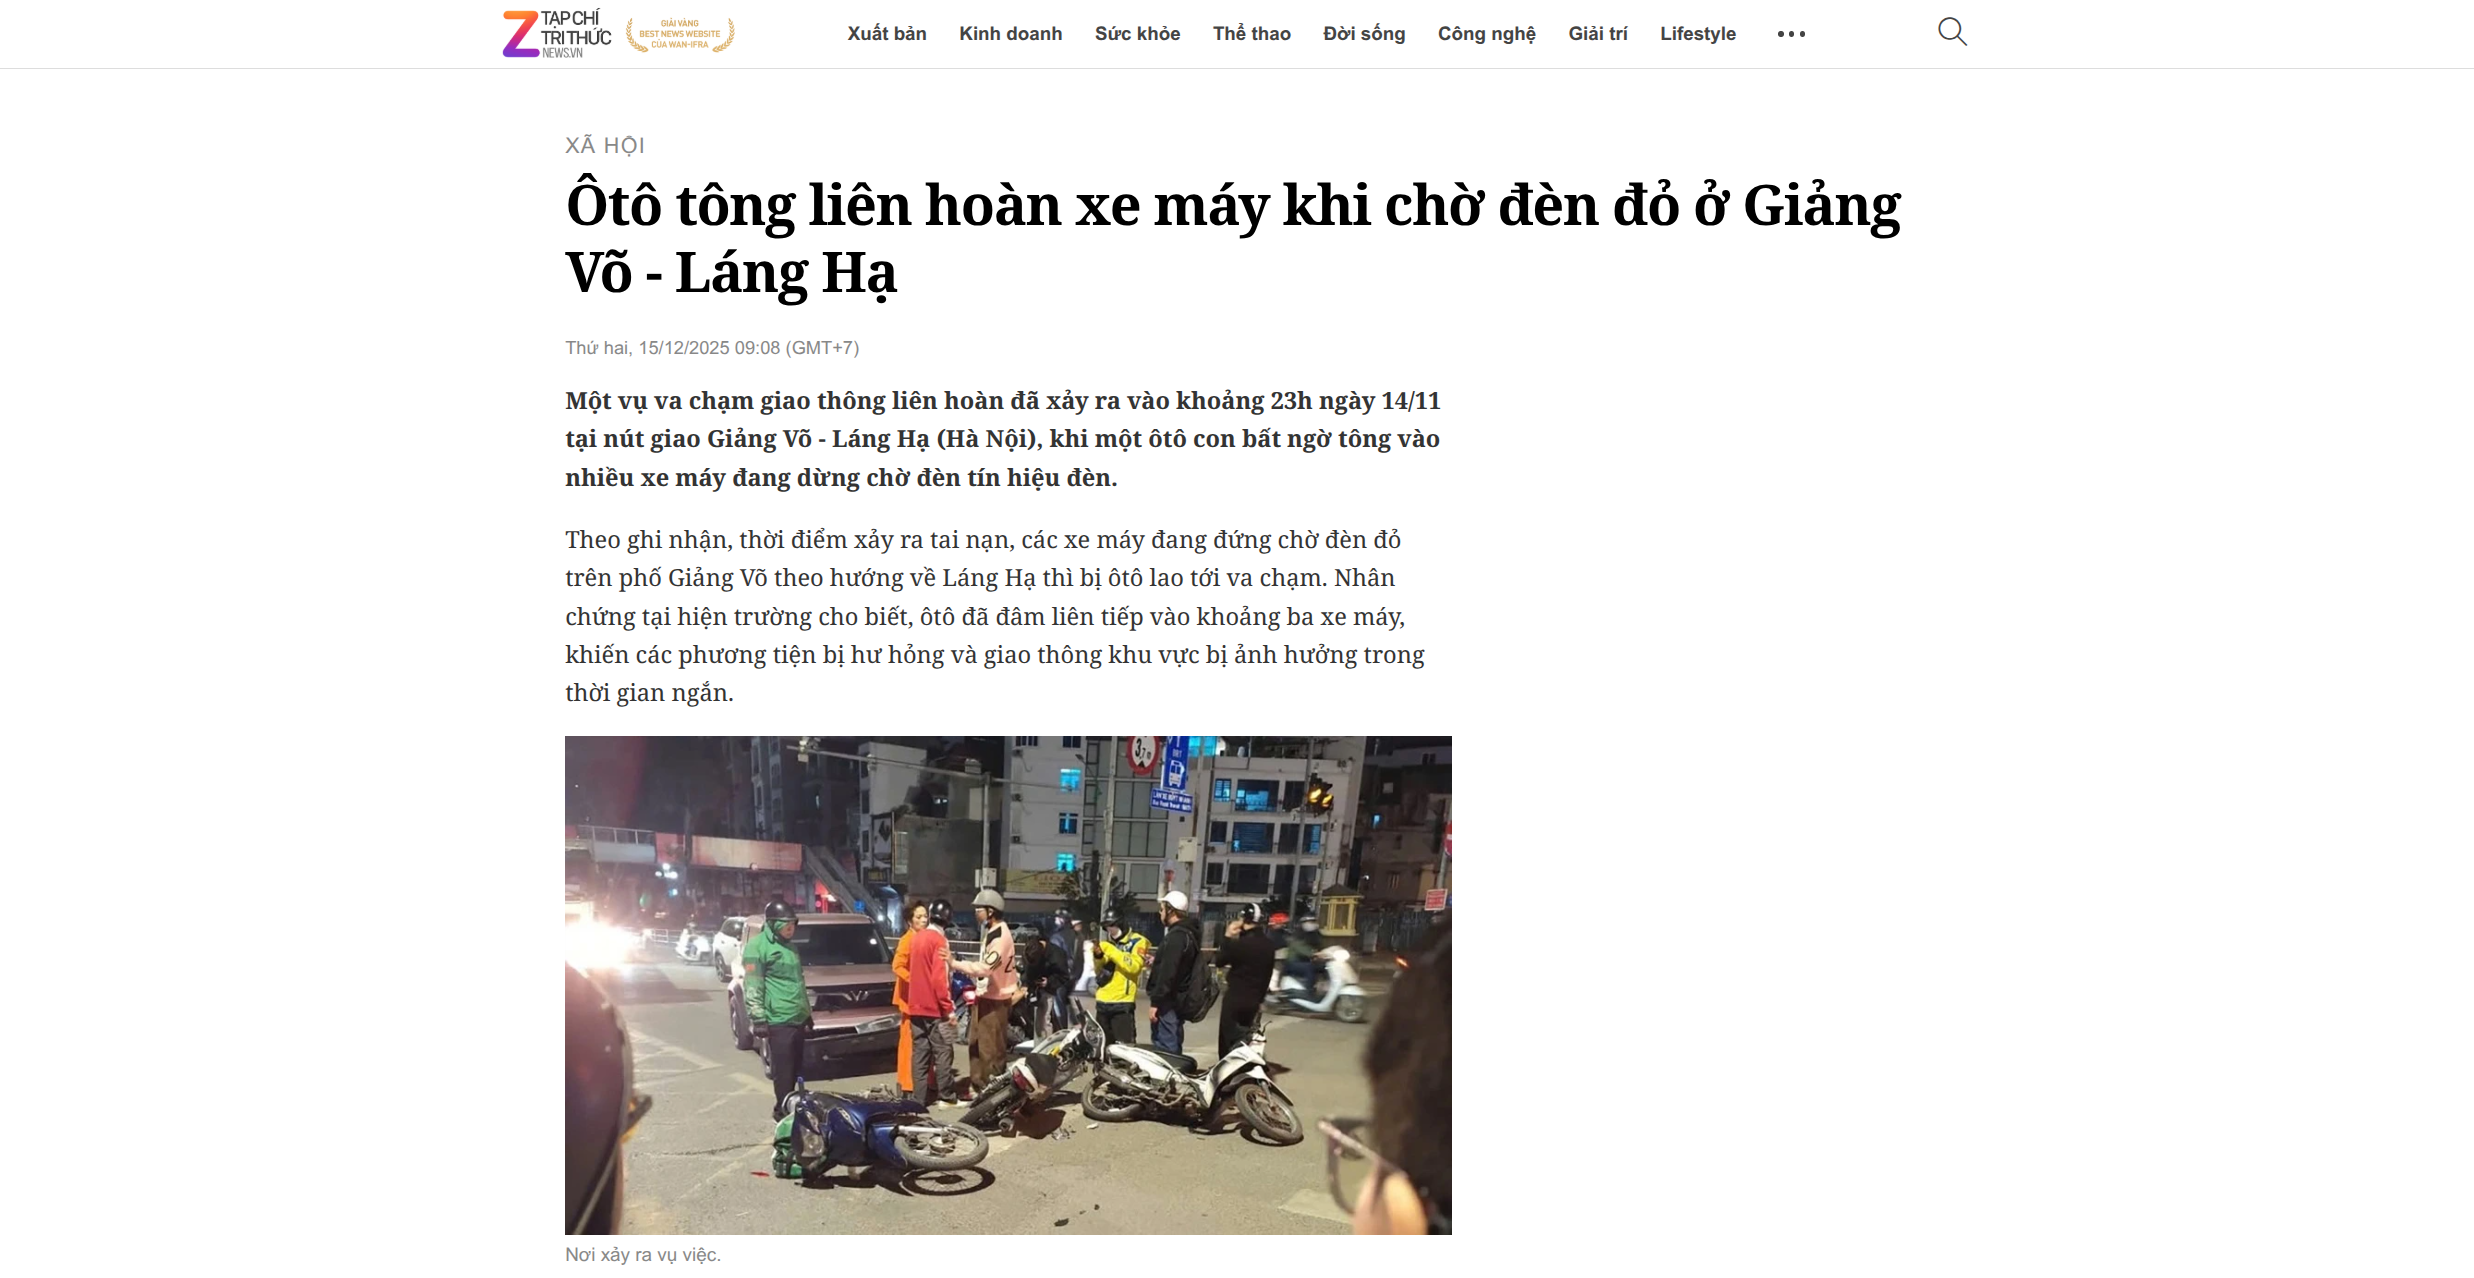
\includegraphics[width=1\textwidth]{Images/znews.png}
    \vspace{0.5cm}
    \caption{A traffic accident caused by red-light violation at an urban intersection in Vietnam on December, 15\textsuperscript{th}, 2025}
    \label{fig:red_light_accident}
\end{figure}

Driver distraction has become an increasingly serious issue in modern traffic environments. The widespread use of mobile devices, in-vehicle infotainment systems, and navigation displays contributes to reduced driver attention. Even brief lapses in concentration can delay reaction time by several hundred milliseconds, which is often sufficient to cause an accident at intersections. Previous studies have shown that delayed reaction, rather than excessive speed alone, is a major contributing factor in red-light-related collisions.

These realities indicate that traditional traffic enforcement and passive safety measures are insufficient to fully address the complexity of modern traffic risks. As a result, there is a growing demand for intelligent driver assistance systems that can actively monitor intersection conditions and provide timely warnings to drivers before dangerous situations escalate.


\subsection{Evolution of Driver Assistance Systems}

Automotive safety systems have evolved significantly over the past decades. Early vehicle safety technologies primarily focused on passive protection mechanisms such as seat belts, airbags, and reinforced vehicle structures. While these systems are effective in reducing injury severity during accidents, they do not actively prevent accidents from occurring.

The emergence of Advanced Driver Assistance Systems (ADAS) marked a shift toward proactive safety solutions. ADAS technologies aim to detect potential hazards, assist drivers in maintaining control, and reduce the likelihood of collisions. Examples include adaptive cruise control, lane departure warning, forward collision warning, and automatic emergency braking. These systems rely heavily on sensor data, including cameras, radar, and lidar, to perceive the driving environment.

Among ADAS components, perception systems play a central role. They are responsible for interpreting raw sensor data and extracting meaningful information such as object positions, traffic signs, lane markings, and traffic signals. With the rapid advancement of artificial intelligence, particularly deep learning and computer vision, perception systems have achieved remarkable improvements in accuracy and robustness.

The automotive industry is currently transitioning toward intelligent and partially autonomous vehicles. This transition requires software architectures capable of supporting complex algorithms, high computational workloads, and dynamic software updates. Consequently, modern vehicle platforms increasingly adopt service-oriented and adaptive software frameworks, such as Adaptive AUTOSAR, to manage the growing complexity of in-vehicle applications.

\subsection{Motivation for Red-Light Warning Systems}

As mentioned previously, intersections represent one of the most hazardous locations in road networks due to the convergence of multiple traffic streams. Accidents occurring at intersections often result in severe injuries, particularly because of lateral impacts and high relative speeds. Consequently, improving safety at intersections has become a priority for traffic authorities and vehicle manufacturers alike.

To address this safety concern, red-light warning systems have been introduced as an effective driver assistance function. These systems are designed to alert drivers when a vehicle approaches an intersection during a red signal phase. By providing early warnings, red-light warning systems can reduce abrupt braking, prevent unintentional signal violations, and lower the risk of high-impact collisions. This capability is especially valuable in situations where driver attention is compromised or visibility is limited.

However, the effectiveness of conventional red-light warning systems is often constrained by the limitations of traditional rule-based traffic light detection methods. Approaches based on fixed color thresholds or geometric assumptions tend to be sensitive to illumination changes, weather conditions, and visual occlusions. In response to these challenges, the application of artificial intelligence to traffic light recognition has gained increasing attention. AI methods are capable of learning complex visual patterns and adapting to diverse real-world conditions, which is essential in highly dynamic traffic environments such as those found in Vietnam.

Beyond perception accuracy, the deployment of red-light warning systems in real vehicles also requires a scalable and maintainable software architecture. Integrating AI perception modules within an Adaptive AUTOSAR framework provides such capabilities by supporting service-oriented communication, dynamic deployment, and high-performance computing. From a system-level perspective, these architectural features strongly motivate the exploration of AI-driven red-light warning systems implemented on Adaptive AUTOSAR platforms to enhance road safety and reduce traffic accidents.

% % \section{Problem Statement}

% % \subsection{Problem Definition}

% % The rapid increase in traffic density and the complexity of urban road environments have made real-time traffic perception a critical requirement for modern vehicles. One of the most challenging and safety-critical perception tasks is the detection of traffic lights, particularly red signals at intersections. Failure to correctly perceive and react to red traffic lights can lead to severe collisions, especially side-impact crashes, which often result in serious injuries or fatalities.

% % The core problem addressed in this research is the design and implementation of a real-time red-light detection and driver warning system for Advanced Driver Assistance Systems (ADAS). The system must accurately recognize traffic lights from camera input, determine the current signal state, and issue timely warnings to the driver when a red-light violation is likely to occur. This process must be completed within strict time constraints to ensure that the warning is meaningful and actionable.

% % Unlike offline image recognition tasks, traffic light detection in real driving scenarios is subject to continuous changes in vehicle speed, viewing angle, illumination conditions, and surrounding traffic. The system must operate reliably under daytime and nighttime conditions, during adverse weather, and in visually cluttered urban environments. Furthermore, false positives and false negatives can both have serious consequences, either by distracting the driver unnecessarily or by failing to warn in genuinely dangerous situations.

% % In addition to perception accuracy, the system must comply with the constraints of in-vehicle embedded platforms. Automotive systems typically have limited computational resources compared to desktop or cloud environments. Therefore, the problem extends beyond algorithm design to include efficient system integration, resource management, and real-time execution within a constrained hardware and software environment.

% % \subsection{Real-Time Requirements in Driving Scenarios}

% % Real-time performance is a fundamental requirement for any safety-related ADAS function. In the context of red-light warning, the system must detect the traffic signal and generate an alert before the vehicle reaches the stop line. Even a small delay in processing can significantly reduce the effectiveness of the warning, particularly at higher vehicle speeds.

% % For example, at a speed of 50 km/h, a vehicle travels approximately 14 meters per second. A processing delay of only 300 milliseconds may result in a positional error of more than four meters, which could be the difference between safe stopping and entering an intersection during a red phase. As a result, the end-to-end latency—from image capture to driver notification—must be strictly bounded.

% % This requirement imposes constraints on all system components, including image acquisition, AI inference, decision logic, and communication between software modules. The system must maintain consistent performance across varying workloads and avoid unpredictable delays caused by resource contention or inefficient scheduling. These real-time constraints present a significant challenge, particularly when deploying computationally intensive AI models on embedded hardware.

% % \subsection{Constraints of In-Vehicle Systems}

% % Automotive embedded systems operate under a set of constraints that differ substantially from general-purpose computing environments. These constraints include limited processing power, restricted memory capacity, and strict energy consumption requirements. Additionally, automotive software must comply with safety, reliability, and maintainability standards throughout the vehicle lifecycle.

% % In many research prototypes, traffic light detection algorithms are developed and evaluated on high-performance workstations or cloud servers. However, such platforms are not representative of real in-vehicle systems. Deploying AI-based perception algorithms in production vehicles requires careful consideration of hardware limitations and system integration challenges.

% % Moreover, automotive software architectures impose additional constraints on how applications are developed and deployed. Adaptive AUTOSAR, for example, introduces standardized mechanisms for application lifecycle management, communication, and service discovery. While these features provide flexibility and scalability, they also require developers to adhere to specific design patterns and interfaces. Consequently, the problem addressed in this work includes not only the development of an effective detection algorithm but also its seamless integration into an Adaptive AUTOSAR-based environment.

% % \subsection{Technical Challenges}

% % The implementation of an AI-based red-light warning system faces several technical challenges across multiple layers of the system.

% % \paragraph*{Visual Challenges}

% % Traffic light detection is inherently a visual perception problem, and its performance is strongly influenced by environmental conditions. Variations in lighting, such as strong sunlight, shadows, nighttime illumination, or glare from wet roads, can significantly affect image quality. Weather conditions including rain, fog, and haze further degrade visibility and contrast.

% % In addition, traffic lights may be partially occluded by other vehicles, trees, or infrastructure elements. In dense urban environments, multiple traffic lights may appear in the camera field of view simultaneously, increasing the risk of misclassification. These visual challenges require detection algorithms that are robust and adaptable to a wide range of real-world scenarios.

% % \paragraph*{Camera Placement and Perspective Distortion}

% % The placement of the camera within the vehicle introduces geometric constraints that affect perception accuracy. Traffic lights are often positioned at varying heights and distances relative to the vehicle, leading to changes in apparent size and shape. Perspective distortion becomes more pronounced as the vehicle approaches the intersection, requiring the detection system to handle scale variation effectively.

% % Furthermore, camera calibration errors and vibration caused by road conditions can introduce additional uncertainty. These factors complicate the task of consistently detecting and tracking traffic lights over time.

% % \paragraph*{AI Inference Latency}

% % Deep learning models, while powerful, are computationally intensive. Running such models in real time on embedded platforms presents a significant challenge. High model complexity may result in unacceptable inference latency, violating real-time constraints. Conversely, overly simplified models may sacrifice detection accuracy.

% % Balancing accuracy and speed is therefore a key challenge. Model optimization techniques such as quantization, pruning, and architecture simplification are often required to achieve acceptable performance. However, these techniques may introduce trade-offs that must be carefully evaluated.

% % \paragraph*{Embedded Hardware Limitations}

% % In many prototype systems, AI inference is initially tested in containerized environments such as Docker, running on general-purpose processors. While this approach simplifies development and testing, it does not fully represent deployment on automotive-grade embedded hardware. Embedded platforms may lack hardware acceleration or have limited support for certain AI frameworks.

% % In the context of this project, the system has primarily been deployed and evaluated on a Raspberry Pi platform, which imposes additional limitations on scalability and performance. These constraints highlight the need for efficient system design and careful resource management.

% % \paragraph*{Safety and Reliability Requirements}

% % ADAS functions are inherently safety-critical, as incorrect behavior may directly endanger human life. The red-light warning system must therefore be reliable, predictable, and resilient to faults. The system should avoid sudden failures and degrade gracefully in the presence of errors or unexpected conditions.

% % Ensuring safety also involves minimizing false alarms, which can lead to driver annoyance and reduced trust in the system. At the same time, missed detections must be minimized to avoid unmitigated hazardous situations. Achieving an appropriate balance between sensitivity and reliability is a central challenge in system design.

% % \subsection{System-Level Requirements}

% % To address the identified challenges, the proposed system must satisfy a set of system-level requirements.

% % \paragraph*{Functional Requirements}

% % The system must be capable of detecting traffic lights from camera input, accurately classifying their signal states, and identifying red-light conditions relevant to the vehicle’s current trajectory. Upon detecting a potential red-light violation, the system must generate a clear and timely warning to the driver.

% % \paragraph*{Non-Functional Requirements}

% % Beyond functional correctness, the system must meet non-functional requirements related to performance, robustness, and maintainability. Real-time operation is essential, with bounded latency from perception to warning output. The system must remain robust under varying environmental and traffic conditions and maintain stable performance over extended periods of operation.

% % \paragraph*{Real-Time and Latency Constraints}

% % The end-to-end processing pipeline must be designed to meet strict latency constraints. This includes efficient scheduling of AI inference tasks, optimized data communication between software components, and minimal overhead introduced by the underlying middleware. The system must ensure that worst-case execution times remain within acceptable bounds.

% % \paragraph*{Safety and Robustness Considerations}

% % Safety considerations require the system to handle edge cases and unexpected inputs gracefully. Robustness mechanisms, such as confidence thresholds and fallback strategies, may be employed to reduce the risk of incorrect warnings. Integration with Adaptive AUTOSAR further supports safety by providing standardized lifecycle management and communication mechanisms suitable for automotive applications.

% % Overall, the problem addressed in this work is a multi-dimensional challenge that spans perception accuracy, real-time performance, embedded system constraints, and automotive software architecture integration. Addressing these aspects in a unified framework is essential for developing a practical and reliable red-light warning system for real-world ADAS deployment.


% \section{System Requirements}

% Based on the identified problem context and technical challenges, the proposed red-light warning system must satisfy a comprehensive set of system requirements. These requirements are structured to cover functional behavior, real-time constraints, perception performance, embedded deployment limitations, safety considerations, and software architecture compliance.

% \subsection{Functional Requirements}

% The system shall provide core ADAS functionality related to red-light awareness and driver warning. Specifically, the system must satisfy the following functional requirements:

% \begin{enumerate}
%     \item The system shall acquire visual input from an camera and process image data in real time.
%     \item The system shall detect traffic lights appearing in the camera field of view.
%     \item The system shall classify detected traffic lights into signal states, including red, yellow, and green.
%     % \item The system shall identify red-light conditions that are relevant to the vehicle’s current driving trajectory.
%     \item The system shall generate a clear and timely warning to the driver when a potential red-light violation is detected in the vehicle range.
%     \item The system shall detect the counter signals from the traffic lights.
    
% \end{enumerate}

% \subsection{Real-Time and Latency Requirements}

% Given the safety-critical nature of red-light warning, strict real-time performance must be guaranteed. The following latency-related requirements are defined:

% \begin{enumerate}
%     \item The end-to-end processing latency, from image acquisition to warning output, shall be bounded and predictable.
%     \item The system shall generate warnings sufficiently early to allow meaningful driver reaction before reaching the stop line.
%     \item The system shall maintain consistent performance across varying vehicle speeds and traffic conditions.
%     \item Processing delays introduced by AI inference, decision logic, and inter-process communication shall not violate real-time constraints.
% \end{enumerate}

% % \subsection{Perception Accuracy and Robustness Requirements}

% % Reliable perception is essential to avoid both missed detections and false alarms. The perception subsystem must satisfy the following requirements:

% % \begin{enumerate}
% %     \item The system shall reliably detect traffic lights under varying illumination conditions, including daytime and nighttime scenarios.
% %     \item The system shall remain robust against visual disturbances such as shadows, glare, and partial occlusion.
% %     \item The system shall handle multiple traffic lights appearing simultaneously in complex urban environments.
% %     \item The system shall minimize false positive detections that could cause unnecessary driver distraction.
% %     \item The system shall minimize false negative detections that could lead to unmitigated hazardous situations.
% % \end{enumerate}

% \subsection{Embedded Platform and Resource Constraints}

% The proposed system is intended for in-vehicle deployment and must operate within the limitations of embedded hardware platforms. The following constraints are therefore imposed:

% \begin{enumerate}
%     \item The system shall operate within limited CPU and memory resources typical of automotive embedded platforms.
%     \item The AI inference pipeline shall be optimized to balance detection accuracy and computational efficiency.
%     \item The system shall avoid excessive energy consumption that could impact overall vehicle operation.
%     \item The system shall support deployment on resource-constrained platforms such as single-board computers used in prototyping.
% \end{enumerate}

% \subsection{Software Architecture and Integration Requirements}

% To ensure maintainability and scalability, the system must comply with automotive software architecture standards. The following integration requirements are defined:

% \begin{enumerate}
%     \item The system shall be implemented within an Adaptive AUTOSAR–based architecture.
%     \item Application components shall communicate through standardized, service-oriented interfaces.
%     \item Application lifecycle management, including startup, execution, and termination, shall follow Adaptive AUTOSAR mechanisms.
%     \item Inter-process communication shall be realized using automotive-grade middleware suitable for real-time operation.
% \end{enumerate}

% \subsection{Safety and Reliability Requirements}

% As an ADAS function, the system must adhere to safety-oriented design principles. The following safety and reliability requirements are imposed:

% \begin{enumerate}
%     \item The system shall exhibit predictable and deterministic behavior during runtime execution.
%     \item The system shall degrade gracefully in the presence of sensor errors, communication failures, or unexpected inputs.
%     \item The system shall avoid abrupt or unsafe system responses that could confuse or endanger the driver.
%     \item The system shall support diagnostic and logging mechanisms to facilitate monitoring, debugging, and validation.
% \end{enumerate}

% Overall, these requirements define the technical and architectural foundation of the proposed red-light warning system. They serve as guiding constraints for system design, implementation, and evaluation, ensuring that the prototype addresses not only perception accuracy but also real-time performance, embedded deployment feasibility, and automotive software integration.


\section{System Requirements}

Based on the identified problem context and technical challenges, the proposed red-light warning system must satisfy a comprehensive set of system requirements. These requirements are structured to cover functional behavior, real-time constraints, perception performance, embedded deployment limitations, safety considerations, and software architecture compliance. Table~\ref{tab:rq_purpose_requirements} summarizes the relationship between the main research questions and the purpose of each requirement group.

\begin{table}[H]
\centering
\renewcommand{\arraystretch}{1.35}
\begin{tabular}{|p{0.43\textwidth}|p{0.50\textwidth}|}
\hline
\textbf{Research Question} & \textbf{Purpose and Derived Requirement} \\
\hline
\textbf{RQ1:} How can a red-light warning system detect traffic lights and countdown timers from camera input? & Define the core perception requirement: the system must detect traffic lights, classify signal colors, recognize countdown timers, and associate the result with the vehicle driving direction. \\
\hline
\textbf{RQ2:} Is there any supporting system that can assist camera-based detection when the vehicle is moving too fast for vision-only perception to be reliable? & Define the GPS-assisted triggering requirement: the system must use GPS and traffic-light node information to estimate the distance to the nearest intersection, determine when the vehicle enters a predefined warning range, and activate camera-based AI perception only when the traffic light becomes relevant to the driving situation. \\
\hline
\textbf{RQ3:} What frame rate is acceptable for an embedded ADAS prototype? & Define the real-time performance requirement: the system should achieve at least {15 FPS} to provide sufficiently smooth and timely warning behavior for an embedded ADAS prototype. \\
\hline
\textbf{RQ4:} How can the system provide timely and useful warning information to the driver? & Define the safety and HMI requirement: the system must display clear warning information, including traffic-light state, countdown timer, node ID, distance, and in-range status, early enough for driver reaction. \\
\hline
\textbf{RQ5:} How can the prototype be integrated into an automotive software architecture? & Define the integration requirement: the system must separate Provider and Client responsibilities, use service-oriented communication middleware, support service discovery, and follow Adaptive AUTOSAR lifecycle concepts. \\
\hline
\textbf{RQ6:} How can the system remain reliable under embedded platform constraints? & Define the resource and reliability requirement: the system must balance AI accuracy and inference latency, avoid excessive CPU and memory usage, provide diagnostic logging, and degrade safely under sensor or communication failures. \\
\hline
\end{tabular}
\caption{Research questions and derived system requirement purposes}
\label{tab:rq_purpose_requirements}
\end{table}

Based on these research questions, the following subsections translate the project goals into concrete functional, timing, resource, integration, and safety requirements.

\subsection{Functional Requirements}

To address \textbf{RQ1}, \textbf{RQ2}, and \textbf{RQ4}, the system is designed to provide comprehensive ADAS functionality tailored to red-light awareness. Primarily, it acquires visual data from an onboard camera and processes it in real time. However, to optimise this process, it actively relies on GPS and node information to calculate the distance to the nearest intersection. Consequently, the camera-based perception pipeline is only activated when the vehicle enters a predefined warning range, directly answering the need for a supporting system (\textbf{RQ2}). Once active, the system detects traffic lights, associates them with specific driving directions (such as turning or going straight), classifies their current signal states, and reads any accompanying countdown timers (\textbf{RQ1}). Finally, to fulfil the human-machine interface demands (\textbf{RQ4}), the system displays this critical information---including node IDs, distances, and timer values---and issues clear, timely driver alerts when a red-light violation is imminent.

\subsection{Real-Time and Latency Requirements}

Responding directly to \textbf{RQ3} and further supporting \textbf{RQ4}, strict real-time performance is a non-negotiable aspect of this safety-critical application. The entire processing pipeline, from image capture to the final warning output, is heavily bounded to ensure predictable latency. To provide a smooth and effective warning experience for the driver, the system is mandated to achieve a minimum processing rate of 15 frames per second (\textbf{RQ3}). This throughput ensures that alerts are generated early enough to allow for meaningful driver reactions before the vehicle crosses the stop line. Furthermore, the architecture guarantees consistent performance regardless of fluctuating vehicle speeds or varying traffic densities, ensuring that delays from AI inference or inter-process communication do not compromise the system's real-time integrity.

% \subsection{Perception Accuracy and Robustness Requirements}

% Reliable perception is essential to avoid both missed detections and false alarms. The perception subsystem must satisfy the following requirements:

% \begin{enumerate}
%     \item The system shall reliably detect traffic lights under varying illumination conditions, including daytime and nighttime scenarios.
%     \item The system shall remain robust against visual disturbances such as shadows, glare, and partial occlusion.
%     \item The system shall handle multiple traffic lights appearing simultaneously in complex urban environments.
%     \item The system shall minimize false positive detections that could cause unnecessary driver distraction.
%     \item The system shall minimize false negative detections that could lead to unmitigated hazardous situations.
% \end{enumerate}

\subsection{Embedded Platform and Resource Constraints}

To tackle the challenges raised by \textbf{RQ6}, the proposed system is strictly tailored for in-vehicle deployment on resource-constrained embedded hardware. Unlike high-end servers, automotive platforms possess limited computational power and memory capacity, necessitating highly optimised AI inference pipelines that strike a careful balance between detection accuracy and processing efficiency. Additionally, the system must avoid excessive power consumption that could negatively impact the overall energy management of the vehicle. By adhering to these constraints, the design ensures seamless deployment on typical prototyping single-board computers while maintaining operational stability.

\subsection{Software Architecture and Integration Requirements}

Addressing \textbf{RQ5}, the system must be constructed in full compliance with modern automotive software standards to guarantee long-term maintainability and scalability. Consequently, the entire prototype is integrated into an Adaptive AUTOSAR framework. This implies that all application components interact exclusively via standardized, service-oriented interfaces and utilize automotive-grade middleware to facilitate reliable inter-process communication. Furthermore, the management of the application's lifecycle---including its startup, execution phases, and termination---strictly follows Adaptive AUTOSAR specifications, ensuring that the software behaves predictably within a complex vehicular network.

\subsection{Safety and Reliability Requirements}
Crucially, safety and reliability represent the most important aspects of this entire project. Addressing both \textbf{RQ5} and \textbf{RQ6}, the system must adhere to stringent safety-oriented design principles inherent to any ADAS function, specifically guided by the ISO 26262 functional safety standard. To achieve this high level of reliability, the system leverages the Adaptive AUTOSAR framework (\textbf{RQ5}), which provides the essential architectural mechanisms to ensure highly deterministic behaviour during runtime. This standard-compliant integration allows the system to degrade gracefully if it encounters sensor malfunctions, communication dropouts, or anomalous inputs. By explicitly avoiding sudden or unsafe responses, the system prevents driver confusion and mitigates potential hazards. Furthermore, comprehensive diagnostic and logging mechanisms are incorporated to enable continuous monitoring and rigorous validation, guaranteeing a fail-safe deployment lifecycle.

Overall, these requirements define the technical and architectural foundation of the proposed red-light warning system. They serve as guiding constraints for system design, implementation, and evaluation, ensuring that the prototype addresses not only perception accuracy but also real-time performance, embedded deployment feasibility, and automotive software integration.

% \section{Scope and Objectives of the Project}

% \subsection{Project Scope}

% The scope of this project is defined to address the problem of red-light violation prevention through an AI-based driver assistance function, while maintaining a practical and realistic implementation target. The project focuses on the development of a perception-driven warning system rather than a fully autonomous control solution. This design choice reflects the current deployment maturity of ADAS technologies and aligns with safety regulations that emphasize driver responsibility.

% At the functional level, the project concentrates on traffic light perception using camera-based input. The system is designed to detect traffic lights in the vehicle’s forward field of view, classify their signal states, and identify red-light conditions relevant to the vehicle’s driving path. Based on this information, the system generates a warning to alert the driver of a potential violation or hazardous situation at an intersection.

% From a system architecture perspective, the project emphasizes software integration within an Adaptive AUTOSAR framework. Core software components include an AI-based perception module, a decision-making module responsible for evaluating red-light risk, and an interface module for driver notification. Communication between these components follows a service-oriented approach, consistent with Adaptive AUTOSAR design principles.

% The scope of this work also includes the deployment and evaluation of the system on an embedded computing platform representative of in-vehicle environments. While the current implementation primarily targets a Raspberry Pi platform and containerized execution environments such as Docker, the design decisions are made with scalability and portability in mind. This allows future migration to automotive-grade hardware with minimal architectural changes.

% However, several functionalities are intentionally excluded from the scope of this project. The system does not perform vehicle control actions such as braking or throttle intervention. Instead, it operates as a warning-only ADAS function, leaving final control decisions to the human driver. Additionally, the project does not address multi-sensor fusion involving radar or lidar, nor does it cover vehicle-to-infrastructure (V2I) communication. These exclusions help to narrow the focus of the research and ensure feasibility within the given development constraints.

% \subsection{Project Objectives}

% The objectives of this project are derived from the identified problem and the defined scope, with an emphasis on both technical feasibility and practical relevance.

% The first objective is to design and implement an AI-based traffic light detection module capable of operating in real time under diverse environmental conditions. This module must accurately identify traffic lights and classify their signal states, with particular attention to red-light detection. The selected AI model should balance detection accuracy with computational efficiency to meet embedded system constraints.

% The second objective is to develop a red-light warning mechanism that effectively supports the driver. This includes defining appropriate criteria for warning generation, such as distance to the intersection, vehicle speed, and confidence in detection results. The warning output should be timely, clear, and minimally intrusive, thereby enhancing driver awareness without causing unnecessary distraction.

% The third objective is to integrate the perception and warning components into an Adaptive AUTOSAR-based software architecture. This involves implementing service interfaces, managing application lifecycles, and ensuring reliable communication between software modules. By leveraging Adaptive AUTOSAR, the project aims to demonstrate how modern automotive software platforms can support AI-driven ADAS functions.

% The fourth objective is to evaluate the system’s real-time performance and operational reliability. Key evaluation criteria include inference latency, end-to-end processing delay, and system stability under continuous operation. Although the current implementation is limited to a prototype environment, performance analysis provides valuable insights into the feasibility of deploying such systems in real vehicles.

% Overall, these objectives collectively aim to demonstrate a complete and coherent ADAS prototype that addresses a real-world traffic safety problem. By focusing on perception accuracy, real-time performance, and architectural integration, the project seeks to contribute practical knowledge toward the development of AI-enabled driver assistance systems within an Adaptive AUTOSAR framework.




\section{Scope and Objectives of the Project}

\subsection{Project Scope}

% Project Scope contains: 
% - The system can detect the traffic light signal, and then classify the color of the traffic light signal
% - The system can detect normal state of the traffic light counters (runs normally on 2-digit number)
% - While the system is running, it can detect the nearby traffic light system in Ho Chi Minh city within the radius of 100 meters, which will annouce when the vehicle is approaching a nearby traffic light signal 



The scope of this project is defined to address the problem of red-light violation prevention through an AI-based driver assistance function, while maintaining a practical and realistic implementation target. The project focuses on the development of a perception-driven warning system rather than a fully autonomous control solution. This design choice reflects the current deployment maturity of ADAS technologies and aligns with safety regulations that emphasize driver responsibility.

At the functional level, the project concentrates on traffic light perception using camera-based input. The system is designed to detect traffic lights in the vehicle’s forward field of view, classify their signal states, and identify red-light conditions relevant to the vehicle’s driving path. Because of disadvantages of mono camera, the system should include the GPS to collect the information of intersection based on ITS \cite{Lee2022TrafficLightRecognition}. As a result, the system generates a warning to alert the driver of a potential violation or hazardous situation at an intersection.

From a system architecture perspective, the project emphasizes software integration within an Adaptive AUTOSAR framework. Core software components include an AI-based perception module, a decision-making module responsible for evaluating red-light risk, and an interface module for driver notification. Communication between these components follows a service-oriented approach, consistent with Adaptive AUTOSAR design principles.

The scope of this work also includes the deployment and evaluation of the system on an embedded computing platform representative of in-vehicle environments. While the current implementation primarily targets a edge device and containerized execution environments such as Docker, the design decisions are made with scalability and portability in mind. This allows future migration to automotive-grade hardware with minimal architectural changes.

\subsection{Out-of-Scope Functionality}

To maintain a focused and feasible research scope, several functionalities are explicitly excluded from this project:

\begin{itemize}
    \item \textbf{Collision avoidance and autonomous intervention:}  
    The system does not perform collision avoidance functions, such as automatic emergency braking, throttle control, or steering intervention. It operates strictly as a warning-only ADAS function, leaving all vehicle control actions to the human driver.

    \item \textbf{Automatic speed or braking control:}  
    Although the system may recommend speed reduction in response to detected red-light conditions, it does not directly control braking or vehicle speed. Any form of enforced deceleration or actuation-level control is outside the scope of this work.

    \item \textbf{Night-time illumination enhancement and low-light compensation:}  
    The project does not address advanced image enhancement techniques for night-time driving, such as adaptive exposure control, HDR processing, or infrared-based perception. Detection performance under extreme low-light conditions is therefore not explicitly optimized.

    \item \textbf{Head-Up Display (HUD) or advanced human–machine interfaces:}  
    Driver feedback is limited to basic warning outputs for prototype evaluation purposes. The design and implementation of advanced visualization interfaces, such as HUD integration or augmented reality displays, are not considered.

    \item \textbf{Multi-sensor fusion and V2X communication:}  
    The system relies solely on camera-based perception and does not incorporate radar, lidar, or vehicle-to-infrastructure (V2I) communication. These extensions are considered potential future enhancements rather than part of the current scope.
\end{itemize}

By explicitly defining these exclusions, the project maintains a clear focus on perception-driven red-light warning and Adaptive AUTOSAR-based system integration, ensuring that the proposed implementation remains feasible within the given development constraints.

\subsection{Project Objectives}

The objectives of this project are derived from the identified problem and the defined scope, with an emphasis on both technical feasibility and practical relevance.

The first objective is to design and implement an AI-based traffic light detection module capable of operating in real time. This module must accurately identify traffic lights and classify their signal states, with particular attention to red-light detection. The selected AI model should balance detection accuracy with computational efficiency to meet embedded system constraints.

The second objective is to develop a red-light warning mechanism that effectively supports the driver. This includes defining appropriate criteria for warning generation, such as distance to the intersection, vehicle speed, and confidence in detection results. The warning output should be timely, clear, and minimally intrusive, thereby enhancing driver awareness without causing unnecessary distraction.

The third objective is to integrate the perception and warning components into an Adaptive AUTOSAR-based software architecture. This involves implementing service interfaces, managing application lifecycles, and ensuring reliable communication between software modules. By leveraging Adaptive AUTOSAR, the project aims to demonstrate how modern automotive software platforms can support AI-driven ADAS functions.

The fourth objective is to evaluate the system’s real-time performance and operational reliability. Key evaluation criteria include inference latency, end-to-end processing delay, and system stability under continuous operation. Although the current implementation is limited to a prototype environment, performance analysis provides valuable insights into the feasibility of deploying such systems in real vehicles.

Overall, these objectives aim to demonstrate a complete and coherent ADAS prototype that addresses a real-world traffic safety problem while remaining aligned with practical deployment constraints and current automotive software standards. 

To clarify how these objectives relate to existing research and industrial practice, the following section reviews related works in traffic light detection, embedded AI deployment, Adaptive AUTOSAR, and spatial positioning.

% \chapter{Related Works}

Developing a robust Advanced Driver Assistance System (ADAS) requires a multidisciplinary approach, bridging the gap between modern artificial intelligence and automotive-grade software engineering. To establish a solid foundation for the proposed red-light warning prototype, a comprehensive review of existing literature and technological frameworks is essential. The following sections explore key advancements across four primary domains that directly influence the system's architecture. Initially, the discussion examines current methodologies in traffic light detection, highlighting the transition from traditional image processing to deep learning-based recognition. Subsequently, the practical challenges of deploying these computationally demanding perception models onto hardware-constrained edge devices are analyzed. The focus then shifts to the AUTOSAR Adaptive Platform, which provides the necessary service-oriented infrastructure for modern automotive software. Finally, the integration of GNSS-based spatial positioning is reviewed as a strategic mechanism to trigger and support visual perception pipelines. Together, these areas establish the necessary context to justify the technological decisions made throughout the project's implementation.

\section{Traffic Light Detection}

Traffic light detection is a fundamental perception task for Advanced Driver Assistance Systems (ADAS) and autonomous driving because traffic signal interpretation directly affects vehicle behavior at intersections. Traditional image-processing approaches rely on handcrafted features such as color thresholding, shape analysis, and region filtering. However, these approaches are sensitive to illumination changes, occlusion, background clutter, and camera viewpoint. Recent studies therefore increasingly adopt deep learning-based object detection to localize traffic lights and classify their signal states.

Nguyen et al.~\cite{Nguyen2025TrafficLightMonitoring} present a traffic light monitoring system using artificial intelligence and show that deep learning-based recognition can improve robustness in practical traffic environments. Their work is relevant because it confirms the suitability of AI-based perception for traffic light monitoring. However, it mainly focuses on detection and monitoring performance, while the integration of perception results into an automotive software architecture and an embedded ADAS warning pipeline is less emphasized.

Lee et al.~\cite{Lee2022TrafficLightRecognition} propose a traffic light recognition system for autonomous driving vehicles using a monocular camera combined with Intelligent Transportation System (ITS) information. This work is closely related to the motivation of this project because it shows that camera-only perception may not be sufficient when the traffic light is far away, visually small, or difficult to detect early enough. By incorporating external contextual information, the system can support recognition before visual perception becomes fully reliable. This idea motivates the GPS-assisted triggering strategy in this project, where the vehicle position and traffic-light node database are used to determine when the AI camera pipeline should be activated.

Countdown timer recognition is another related perception problem. Goodfellow et al.~\cite{goodfellow2014multidigitnumberrecognitionstreet} demonstrate that deep convolutional neural networks can recognize multi-digit numbers from real-world street-view imagery. Although their work is not specific to traffic light countdown timers, it provides a strong reference for digit recognition in unconstrained outdoor scenes. This supports the timer OCR component of the proposed system, where countdown values associated with detected traffic lights are recognized and displayed to the user.

\section{Deploying Model on Hardware-Constrained Devices}

A major gap between research prototypes and practical ADAS systems is the deployment of perception models on embedded hardware. Object detection models are often evaluated on desktop GPUs, but in-vehicle systems must satisfy stricter constraints in terms of CPU usage, memory consumption, power consumption, and latency. For a driver warning function, average accuracy alone is insufficient; the model must also provide stable frame rate and bounded processing delay.

MobileNetV4~\cite{qin2024mobilenetv4universalmodels} is engineered specifically for resource-constrained ecosystems, offering an optimal balance between accuracy and computational efficiency. During the first phase of this project, we leveraged this architecture to develop a highly optimized YOLO11n-MobileNetV4 model---formally documented in our IEEE SAS 2026 submission (see \hyperref[chap:append]{Appendix}). Building directly upon the theoretical foundations and structural optimizations established in that paper, the current prototype advances the design by proposing a novel {YOLO26-MobileNetV4} model because YOLO26 is better than YOLOv11 \cite{yolo26}. This evolution aims to further minimize inference latency and maximize real-time feasibility on edge devices.

Goodfellow et al.~\cite{goodfellow2014multidigitnumberrecognitionstreet} also provide useful background for embedded perception because their CNN-based digit recognition approach demonstrates how a focused neural network can solve a specific recognition subtask. In this project, the traffic light detector and the countdown timer recognizer are separated so that the timer OCR task can be handled by a lightweight CNN model rather than by a large general-purpose detection network. This modular design supports the goal of maintaining real-time performance on constrained hardware.

\section{AUTOSAR Adaptive Platform}

The AUTOSAR Adaptive Platform is designed for high-performance automotive applications that require dynamic service-oriented communication, lifecycle management, and execution on POSIX-based operating systems. AUTOSAR documentation describes the Adaptive Platform as a complement to Classic AUTOSAR~\cite{autosar_layered_arch}, targeting applications such as ADAS, automated driving, infotainment, and high-performance computing workloads~\cite{autosar_platform_design,autosar_sw_arch}. This makes it an appropriate architectural foundation for integrating perception, communication, and display functions in the proposed prototype.

Communication Management is a central functional cluster in Adaptive AUTOSAR. It defines how Adaptive Applications communicate through service-oriented interfaces and network bindings such as SOME/IP~\cite{autosar_someip} and DDS~\cite{autosar_com_mgmt, autosar_dds}. Execution Management defines how processes are started, supervised, and coordinated using execution manifests and machine states~\cite{autosar_exec_mgmt}. Log and Trace provides standardized runtime observability for debugging and validation~\cite{autosar_log_trace}. These functional clusters are relevant to this project because the prototype separates the Provider and Client applications, uses middleware-based communication, reports execution state, and relies on logging to evaluate runtime behavior.

The AUTOSAR methodology further defines a configuration-driven workflow in which high-level architecture, service interfaces, application design, machine configuration, and deployment artefacts are refined into executable software~\cite{AUTOSAR_TR_AdaptiveMethodology_R22-11}. PopcornSAR provides AUTOSAR tooling and product support aligned with this configuration-oriented workflow~\cite{popcornsar_intro}. These references form the methodological basis for using Autosar.io to configure the prototype, generate application artefacts, and maintain consistency between design and deployment.

\section{Spatial Positioning with GNSS}

Spatial positioning provides an important complementary layer for traffic light warning systems. A camera can only detect what is visible in its field of view, and its reliability decreases when the traffic light is far away, small, occluded, or affected by lighting conditions. At higher vehicle speeds, waiting until the traffic light is clearly visible may leave insufficient time for warning generation. Therefore, a supporting positioning mechanism is needed to determine whether the vehicle is approaching a relevant traffic-light node before the camera-based detector becomes reliable.

Lee et al.~\cite{Lee2022TrafficLightRecognition} address a similar problem by combining monocular camera recognition with ITS information. Their approach demonstrates the value of using external traffic infrastructure information to support camera-based recognition. In this project, the same principle is adapted using GNSS/GPS and a traffic-light node database. The GPS module estimates the current vehicle position, while the node database provides the locations of signalized intersections. By calculating the distance between the vehicle and the nearest traffic-light node, the system can determine whether the vehicle is inside the warning range and whether the AI perception pipeline should be activated.

Compared with a camera-only warning system, this hybrid design reduces unnecessary inference when the vehicle is far from relevant intersections and improves the chance of producing an early warning when the vehicle approaches a traffic light. Thus, spatial positioning is not used as a replacement for visual perception, but as a triggering and contextual support mechanism that makes the perception pipeline more practical for embedded ADAS deployment.

Based on the gaps identified in these related works, the next section consolidates the chapter and prepares the transition toward the theoretical background required for the proposed implementation.


\subsection{Phase 1 Achievements and Phase 2 Objectives}

\begin{figure}[H]
    \centering
    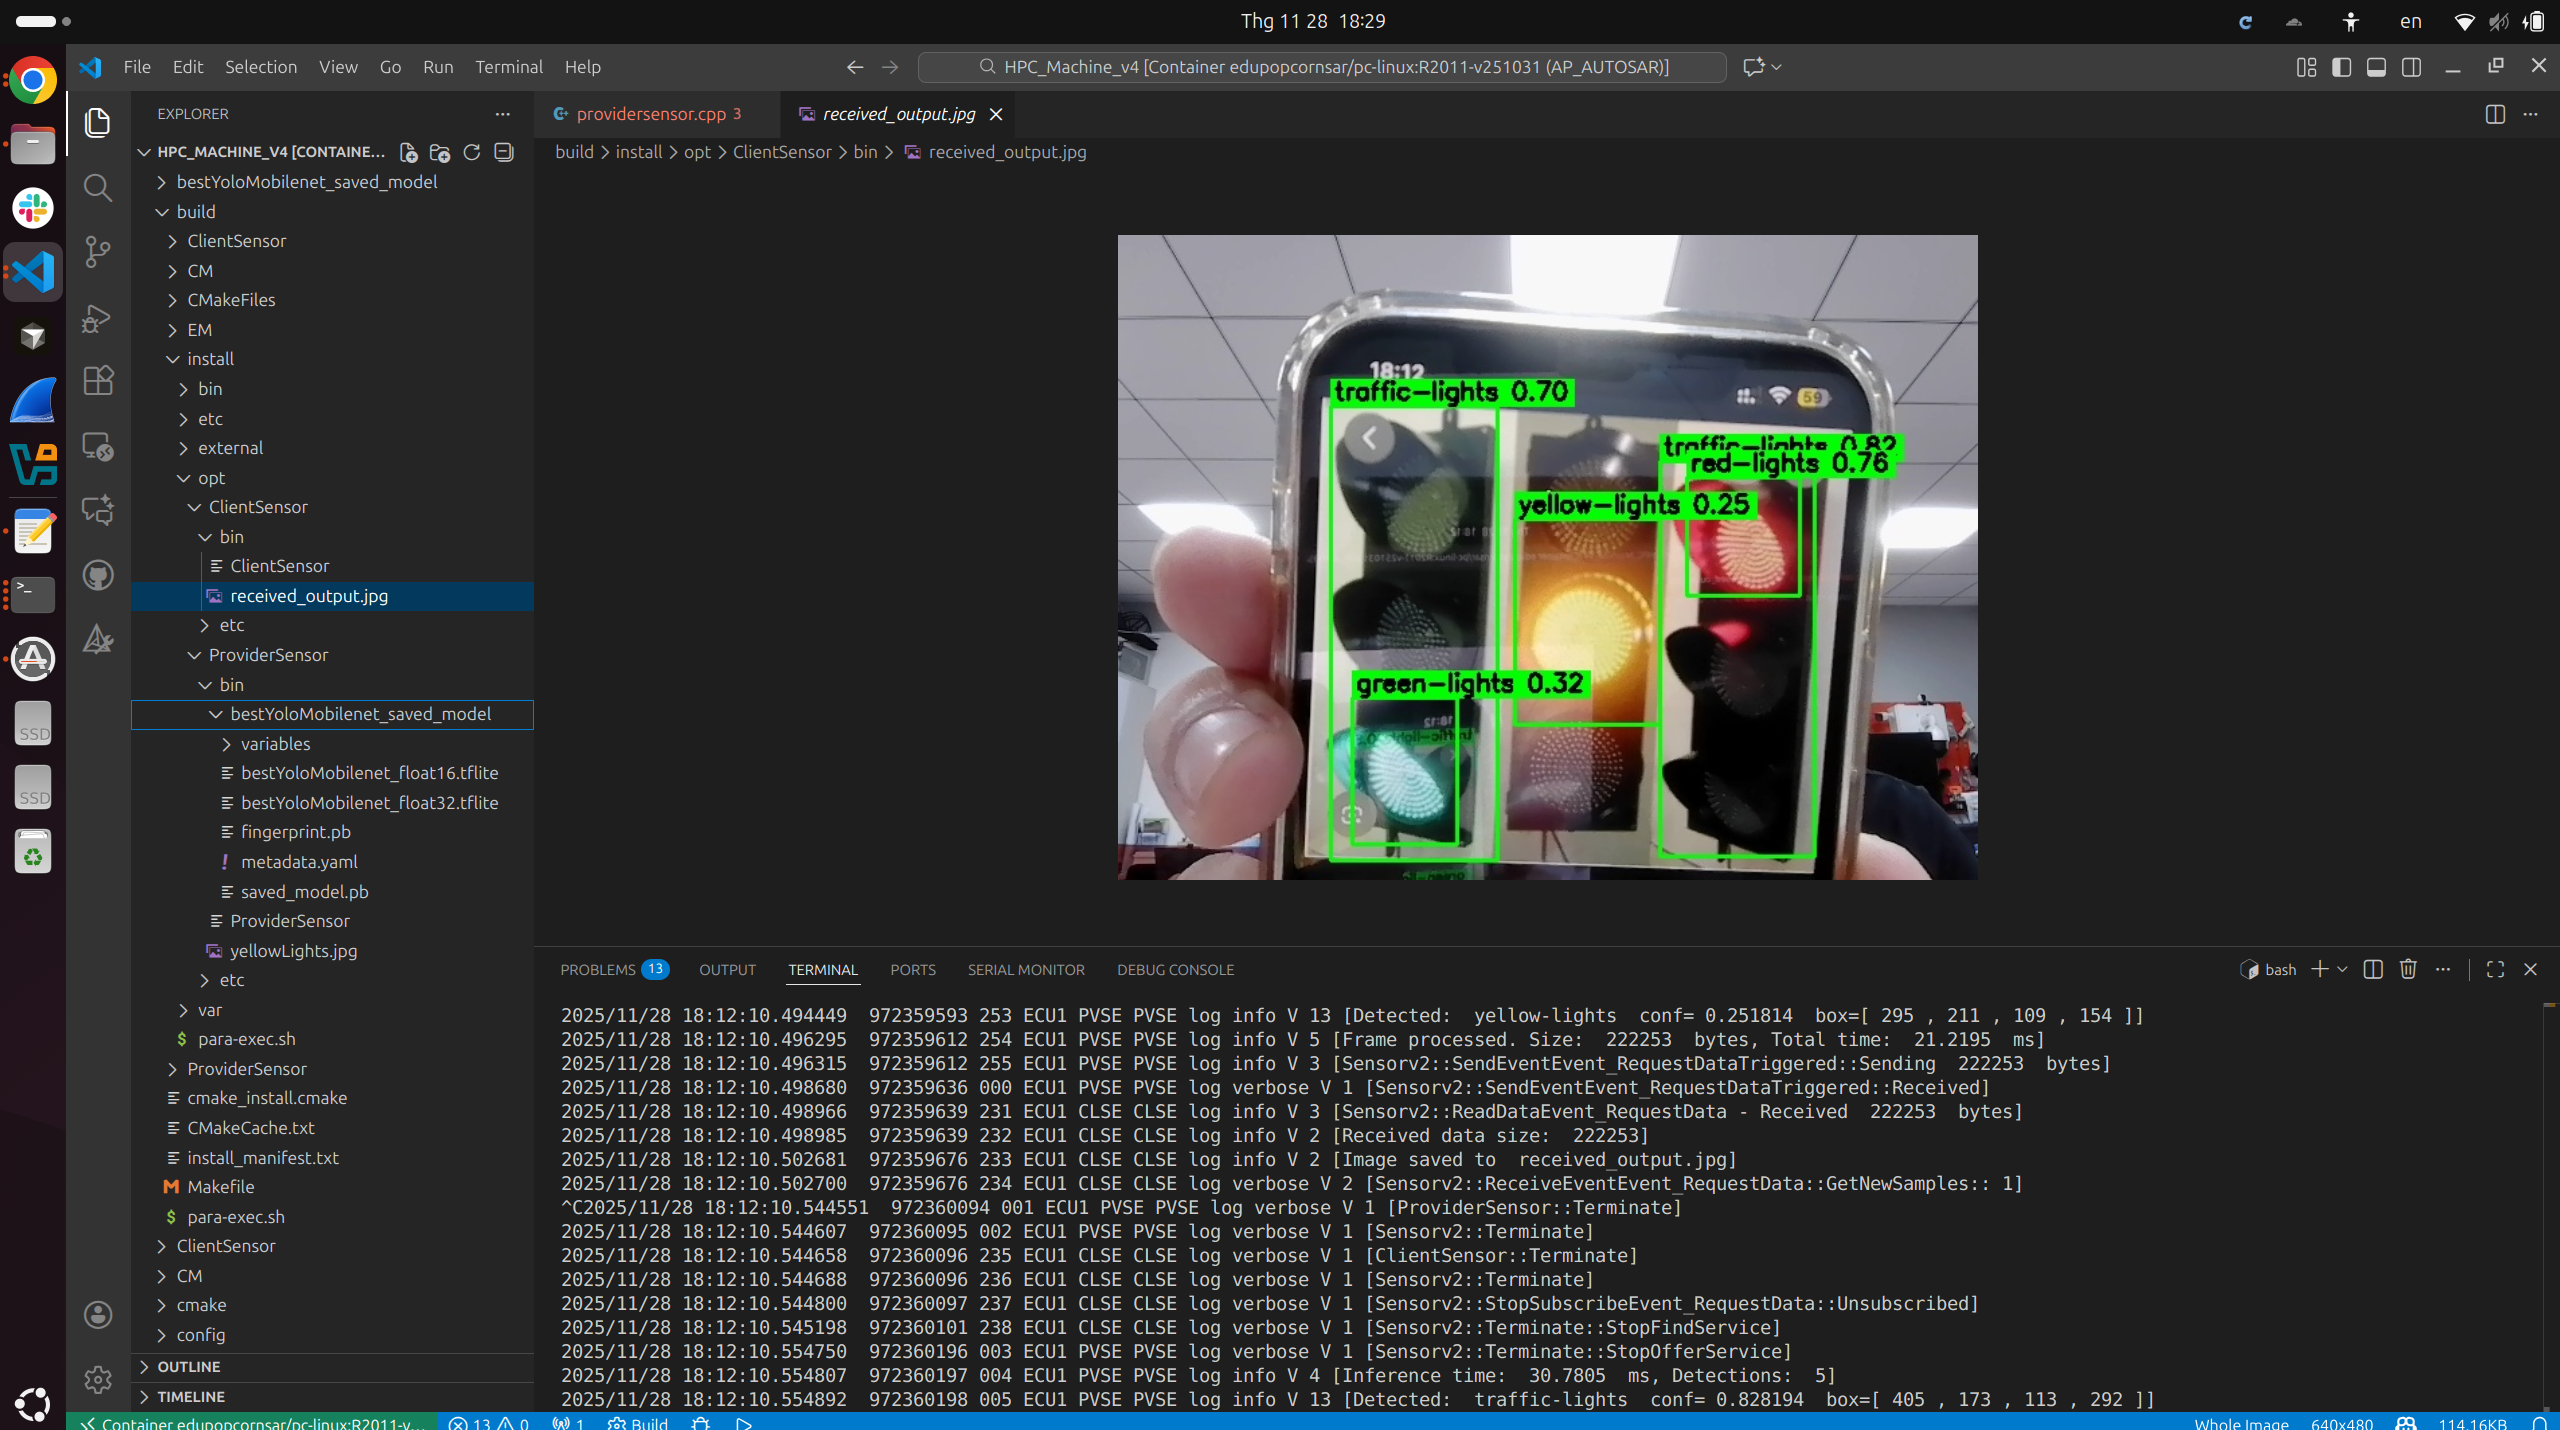
\includegraphics[width=0.75\textwidth]{Images/resultPhrase1.png}
    \vspace{0.5cm}
    \caption{The result of the prototype project in Phase 1}
    \label{fig:res_project_phase1}
\end{figure}

As illustrated in Figure~\ref{fig:res_project_phase1}, the first phase of this project successfully established the foundational architecture for an edge-based perception system. The Adaptive AUTOSAR platform was deployed and executed within a Docker container environment, proving the viability of containerized automotive software. For the visual perception task, a YOLO11n-MobileNetV4 model was utilized to perform basic traffic light detection, limited primarily to identifying red, yellow, and green signal states. The processed sensor data was transmitted seamlessly between applications via the SOME/IP communication middleware, successfully validating the basic service-oriented data flow. Following the successful completion of Phase 1, the core findings and architectural methodologies were compiled into a research paper submitted to the IEEE Sensors Applications Symposium 2026 (IEEE SAS 2026). This manuscript, scheduled for presentation in July 2026, is provided in full in \hyperref[chap:append]{Appendix}.

Building upon that success, the current and final phase of the project significantly upgrades both the software architecture and the perception capabilities. The Adaptive AUTOSAR configuration is transitioned to utilize the Data Distribution Service (DDS) middleware, providing a more robust communication backbone and also following the ADAS standards. The perception pipeline is completely overhauled by replacing the YOLO11 baseline with the newest Ultralytics architecture, chosen specifically for its anchor-free and Non-Maximum Suppression (NMS)-free design. To handle complex intersection data, a custom lightweight multi-head CNN is introduced to explicitly detect countdown timers, while the GPS module is integrated to cross-reference Intelligent Transportation Systems (ITS) nodes for early, predictive warnings. Ultimately, these enhancements expand the detection scope from simple color recognition to identifying specific lane directions, signal colors, and timer values simultaneously, all while maintaining high accuracy and an inference speed of $\geq 15$ frames per second (FPS) in edge device, which completely run on CPU without GPU and NPU. And the next section, we will introduce the contribution and structure of our report.

\section{Contributions and Report Structure}

The preceding sections have established the foundational context for the proposed red-light warning system. By exploring the background of traffic safety and the limitations of current solutions, the core motivation for this project has been clearly defined. Furthermore, the specific system requirements, project scope boundaries, and related research gaps have also been outlined.

To address these identified challenges, this project makes two major technical contributions:
\begin{enumerate}
    \item \textbf{Implementing Adaptive AUTOSAR to Industry Standards:} The project successfully develops and deploys a service-oriented software architecture using the PopcornSAR toolchain. This implementation closely follows modern automotive industry standards, ensuring robust and reliable inter-process communication.
    \item \textbf{Deploying Edge AI on Constrained Hardware:} The project designs a highly optimized, lightweight AI perception pipeline (utilizing a YOLO-MobileNetV4 and multi-head CNN architecture). This pipeline is capable of running efficiently on an edge device to achieve real-time traffic light detection without relying on high-end cloud computing.
\end{enumerate}

With the problem clearly defined and the main contributions established, the remainder of this report is logically structured to guide the reader through the technical development of the project. The subsequent chapters are organized as follows:

\begin{itemize}
    \item \textbf{Chapter 2 (Related Works):} Reviews existing literature to provide a critical context for the research. It explores current traffic light detection methods, the practical challenges of deploying complex AI models on edge devices, and the role of GNSS positioning in modern automotive systems.
    
    \item \textbf{Chapter 3 (Background):} Introduces the fundamental technologies that form the foundation of the project. It clarifies the core concepts of the Adaptive AUTOSAR framework, alongside the selected perception tools such as the YOLO algorithm and the LiteRT inference engine.
    
    \item \textbf{Chapter 4 (System Configuration and Methodology):} Details the software setup and the proposed development workflow. It thoroughly explains the design of service-oriented interfaces, the training processes for the customized YOLO-MobileNetV4 and Multi-head CNN models, and the creation of a reproducible execution environment.
    
    \item \textbf{Chapter 5 (Project Prototype):} Demonstrates the actual hands-on implementation of the ADAS system. It traces the complete data flow from sensor acquisition to the driver display using DDS middleware, while also presenting the final experimental setup and evaluation results.
    
    \item \textbf{Chapter 6 (Conclusion and Future Enhancement of Project):} Concludes the thesis by summarizing the primary achievements and evaluating the system's overall effectiveness. It reflects on the prototype's real-world performance and outlines potential avenues for future research.
\end{itemize}

Together, this structure ensures a clear and comprehensive progression from the initial problem statement to a fully functioning driver assistance system.

\newpage
\chapter{Related Works}

Developing a robust Advanced Driver Assistance System (ADAS) requires a multidisciplinary approach, bridging the gap between modern artificial intelligence and automotive-grade software engineering. To establish a solid foundation for the proposed red-light warning prototype, a comprehensive review of existing literature and technological frameworks is essential. The following sections explore key advancements across four primary domains that directly influence the system's architecture. Initially, the discussion examines current methodologies in traffic light detection, highlighting the transition from traditional image processing to deep learning-based recognition. Subsequently, the practical challenges of deploying these computationally demanding perception models onto hardware-constrained edge devices are analyzed. The focus then shifts to the AUTOSAR Adaptive Platform, which provides the necessary service-oriented infrastructure for modern automotive software. Finally, the integration of GNSS-based spatial positioning is reviewed as a strategic mechanism to trigger and support visual perception pipelines. Together, these areas establish the necessary context to justify the technological decisions made throughout the project's implementation.

\section{Traffic Light Detection}

Traffic light detection is a fundamental perception task for Advanced Driver Assistance Systems (ADAS) and autonomous driving because traffic signal interpretation directly affects vehicle behavior at intersections. Traditional image-processing approaches rely on handcrafted features such as color thresholding, shape analysis, and region filtering. However, these approaches are sensitive to illumination changes, occlusion, background clutter, and camera viewpoint. Recent studies therefore increasingly adopt deep learning-based object detection to localize traffic lights and classify their signal states.

Nguyen et al.~\cite{Nguyen2025TrafficLightMonitoring} present a traffic light monitoring system using artificial intelligence and show that deep learning-based recognition can improve robustness in practical traffic environments. Their work is relevant because it confirms the suitability of AI-based perception for traffic light monitoring. However, it mainly focuses on detection and monitoring performance, while the integration of perception results into an automotive software architecture and an embedded ADAS warning pipeline is less emphasized.

Lee et al.~\cite{Lee2022TrafficLightRecognition} propose a traffic light recognition system for autonomous driving vehicles using a monocular camera combined with Intelligent Transportation System (ITS) information. This work is closely related to the motivation of this project because it shows that camera-only perception may not be sufficient when the traffic light is far away, visually small, or difficult to detect early enough. By incorporating external contextual information, the system can support recognition before visual perception becomes fully reliable. This idea motivates the GPS-assisted triggering strategy in this project, where the vehicle position and traffic-light node database are used to determine when the AI camera pipeline should be activated.

Countdown timer recognition is another related perception problem. Goodfellow et al.~\cite{goodfellow2014multidigitnumberrecognitionstreet} demonstrate that deep convolutional neural networks can recognize multi-digit numbers from real-world street-view imagery. Although their work is not specific to traffic light countdown timers, it provides a strong reference for digit recognition in unconstrained outdoor scenes. This supports the timer OCR component of the proposed system, where countdown values associated with detected traffic lights are recognized and displayed to the user.

\section{Deploying Model on Hardware-Constrained Devices}

A major gap between research prototypes and practical ADAS systems is the deployment of perception models on embedded hardware. Object detection models are often evaluated on desktop GPUs, but in-vehicle systems must satisfy stricter constraints in terms of CPU usage, memory consumption, power consumption, and latency. For a driver warning function, average accuracy alone is insufficient; the model must also provide stable frame rate and bounded processing delay.

MobileNetV4~\cite{qin2024mobilenetv4universalmodels} is engineered specifically for resource-constrained ecosystems, offering an optimal balance between accuracy and computational efficiency. During the first phase of this project, we leveraged this architecture to develop a highly optimized YOLO11n-MobileNetV4 model---formally documented in our IEEE SAS 2026 submission (see \hyperref[chap:append]{Appendix}). Building directly upon the theoretical foundations and structural optimizations established in that paper, the current prototype advances the design by proposing a novel {YOLO26-MobileNetV4} model because YOLO26 is better than YOLOv11 \cite{yolo26}. This evolution aims to further minimize inference latency and maximize real-time feasibility on edge devices.

Goodfellow et al.~\cite{goodfellow2014multidigitnumberrecognitionstreet} also provide useful background for embedded perception because their CNN-based digit recognition approach demonstrates how a focused neural network can solve a specific recognition subtask. In this project, the traffic light detector and the countdown timer recognizer are separated so that the timer OCR task can be handled by a lightweight CNN model rather than by a large general-purpose detection network. This modular design supports the goal of maintaining real-time performance on constrained hardware.

\section{AUTOSAR Adaptive Platform}

The AUTOSAR Adaptive Platform is designed for high-performance automotive applications that require dynamic service-oriented communication, lifecycle management, and execution on POSIX-based operating systems. AUTOSAR documentation describes the Adaptive Platform as a complement to Classic AUTOSAR~\cite{autosar_layered_arch}, targeting applications such as ADAS, automated driving, infotainment, and high-performance computing workloads~\cite{autosar_platform_design,autosar_sw_arch}. This makes it an appropriate architectural foundation for integrating perception, communication, and display functions in the proposed prototype.

Communication Management is a central functional cluster in Adaptive AUTOSAR. It defines how Adaptive Applications communicate through service-oriented interfaces and network bindings such as SOME/IP~\cite{autosar_someip} and DDS~\cite{autosar_com_mgmt, autosar_dds}. Execution Management defines how processes are started, supervised, and coordinated using execution manifests and machine states~\cite{autosar_exec_mgmt}. Log and Trace provides standardized runtime observability for debugging and validation~\cite{autosar_log_trace}. These functional clusters are relevant to this project because the prototype separates the Provider and Client applications, uses middleware-based communication, reports execution state, and relies on logging to evaluate runtime behavior.

The AUTOSAR methodology further defines a configuration-driven workflow in which high-level architecture, service interfaces, application design, machine configuration, and deployment artefacts are refined into executable software~\cite{AUTOSAR_TR_AdaptiveMethodology_R22-11}. PopcornSAR provides AUTOSAR tooling and product support aligned with this configuration-oriented workflow~\cite{popcornsar_intro}. These references form the methodological basis for using Autosar.io to configure the prototype, generate application artefacts, and maintain consistency between design and deployment.

\section{Spatial Positioning with GNSS}

Spatial positioning provides an important complementary layer for traffic light warning systems. A camera can only detect what is visible in its field of view, and its reliability decreases when the traffic light is far away, small, occluded, or affected by lighting conditions. At higher vehicle speeds, waiting until the traffic light is clearly visible may leave insufficient time for warning generation. Therefore, a supporting positioning mechanism is needed to determine whether the vehicle is approaching a relevant traffic-light node before the camera-based detector becomes reliable.

Lee et al.~\cite{Lee2022TrafficLightRecognition} address a similar problem by combining monocular camera recognition with ITS information. Their approach demonstrates the value of using external traffic infrastructure information to support camera-based recognition. In this project, the same principle is adapted using GNSS/GPS and a traffic-light node database. The GPS module estimates the current vehicle position, while the node database provides the locations of signalized intersections. By calculating the distance between the vehicle and the nearest traffic-light node, the system can determine whether the vehicle is inside the warning range and whether the AI perception pipeline should be activated.

Compared with a camera-only warning system, this hybrid design reduces unnecessary inference when the vehicle is far from relevant intersections and improves the chance of producing an early warning when the vehicle approaches a traffic light. Thus, spatial positioning is not used as a replacement for visual perception, but as a triggering and contextual support mechanism that makes the perception pipeline more practical for embedded ADAS deployment.

Based on the gaps identified in these related works, the next section consolidates the chapter and prepares the transition toward the theoretical background required for the proposed implementation.


\newpage
\chapter{Background}

Developing a robust ADAS requires a strong theoretical foundation that bridges automotive middleware, artificial intelligence, and edge computing. The present chapter outlines the core technologies and frameworks employed to construct the proposed prototype, ensuring that all subsequent implementations are grounded in established industry standards. 

To provide a comprehensive overview of the system's underlying technologies, the remainder of the chapter is structured as follows:

\begin{itemize}
    \item \textbf{Adaptive AUTOSAR Architecture:} Explores the primary software backbone (Release R21-11) used for building dynamic, service-oriented automotive applications.
    \item \textbf{Development Toolchains:} Introduces the PopcornSAR toolchain and the PARA SDK Docker environment, detailing how initial code skeletons are generated and executed reliably.
    \item \textbf{YOLO Model and MobileNetV4 Backbone:} Examines the real-time object detection architecture utilized for traffic light localization, emphasizing its lightweight edge-computing design.
    \item \textbf{Google LiteRT Framework:} Details the inference engine (formerly TensorFlow Lite) employed to execute deep learning models efficiently with low latency and a minimal memory footprint.
    \item \textbf{GNSS Integration:} Incorporates Global Navigation Satellite System concepts to enable spatial reasoning and distance estimation, compensating for the limitations of camera-only perception.
    \item \textbf{Hardware:} Presents the physical edge platform, illustrating how the software middleware, AI models, and localization modules operate together cohesively.
\end{itemize}

\section{Adaptive AUTOSAR Architecture}

AUTOSAR (Automotive Open System ARchitecture) is a global development partnership of automotive interested parties. It establishes a standardized software framework and open architecture for automotive Electronic Control Units (ECUs). The primary goal is to facilitate the scalability, transferability, and reusability of software modules across different vehicle platforms. The standard is divided into two major platforms: the Classic Platform and the Adaptive Platform.

The Classic AUTOSAR platform targets deeply embedded systems with stringent real-time and safety constraints. It is optimized for microcontrollers with limited resources and is characterized by a static configuration and direct interaction with hardware peripherals (sensors, actuators) and vehicle networks like CAN and LIN. This platform is the standard for safety-critical functions requiring deterministic execution \cite{autosar_layered_arch}. As in the Figure \ref{fig:autosar_classic_arch}, the Classic Platform is heavily based on the microcontroller hardware. 

\begin{figure}[h]
    \centering
    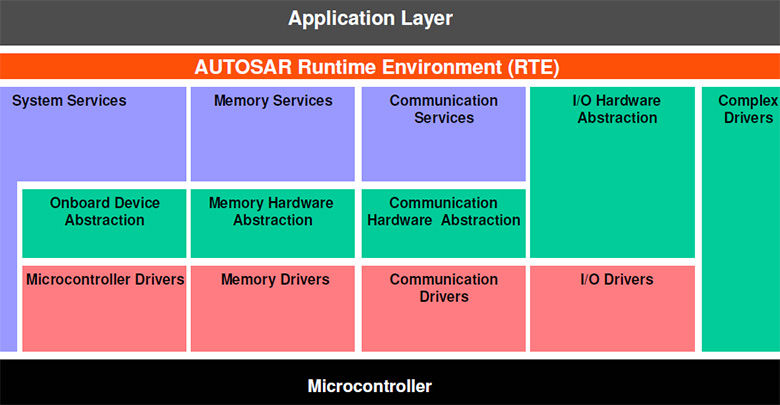
\includegraphics[width=1\textwidth]{Images/chapter2/AR_arch.jpg}
    \vspace{0.5cm}
    \caption{AUTOSAR Classic Architecture}
    \label{fig:autosar_classic_arch}
\end{figure}

However, the increasing complexity of modern automotive systems, particularly in the domains of Advanced Driver Assistance Systems (ADAS) and autonomous driving, demands computational capabilities that exceed the design limits of the Classic Platform. To address these emerging requirements, the Adaptive AUTOSAR platform was introduced. It complements the Classic Platform by providing a flexible, high-performance runtime environment for data-intensive applications and service-oriented architectures, supporting dynamic updates and high-bandwidth communication. However, the Adaptive AUTOSAR platform is not a drop-in replacement for the Classic Platform, it runs parallel to the Classic Platform with other non-AUTOSAR software modules. Rather, it will interact with these platforms and external backend systems such as road-side infrastructures, to form an integrated system. As in Figure \ref{fig:autosar_adaptive_and_classic}, CP already incorporates SOME/IP, which is also supported by AP, among other protocols.

\begin{figure}[h]
    \centering
    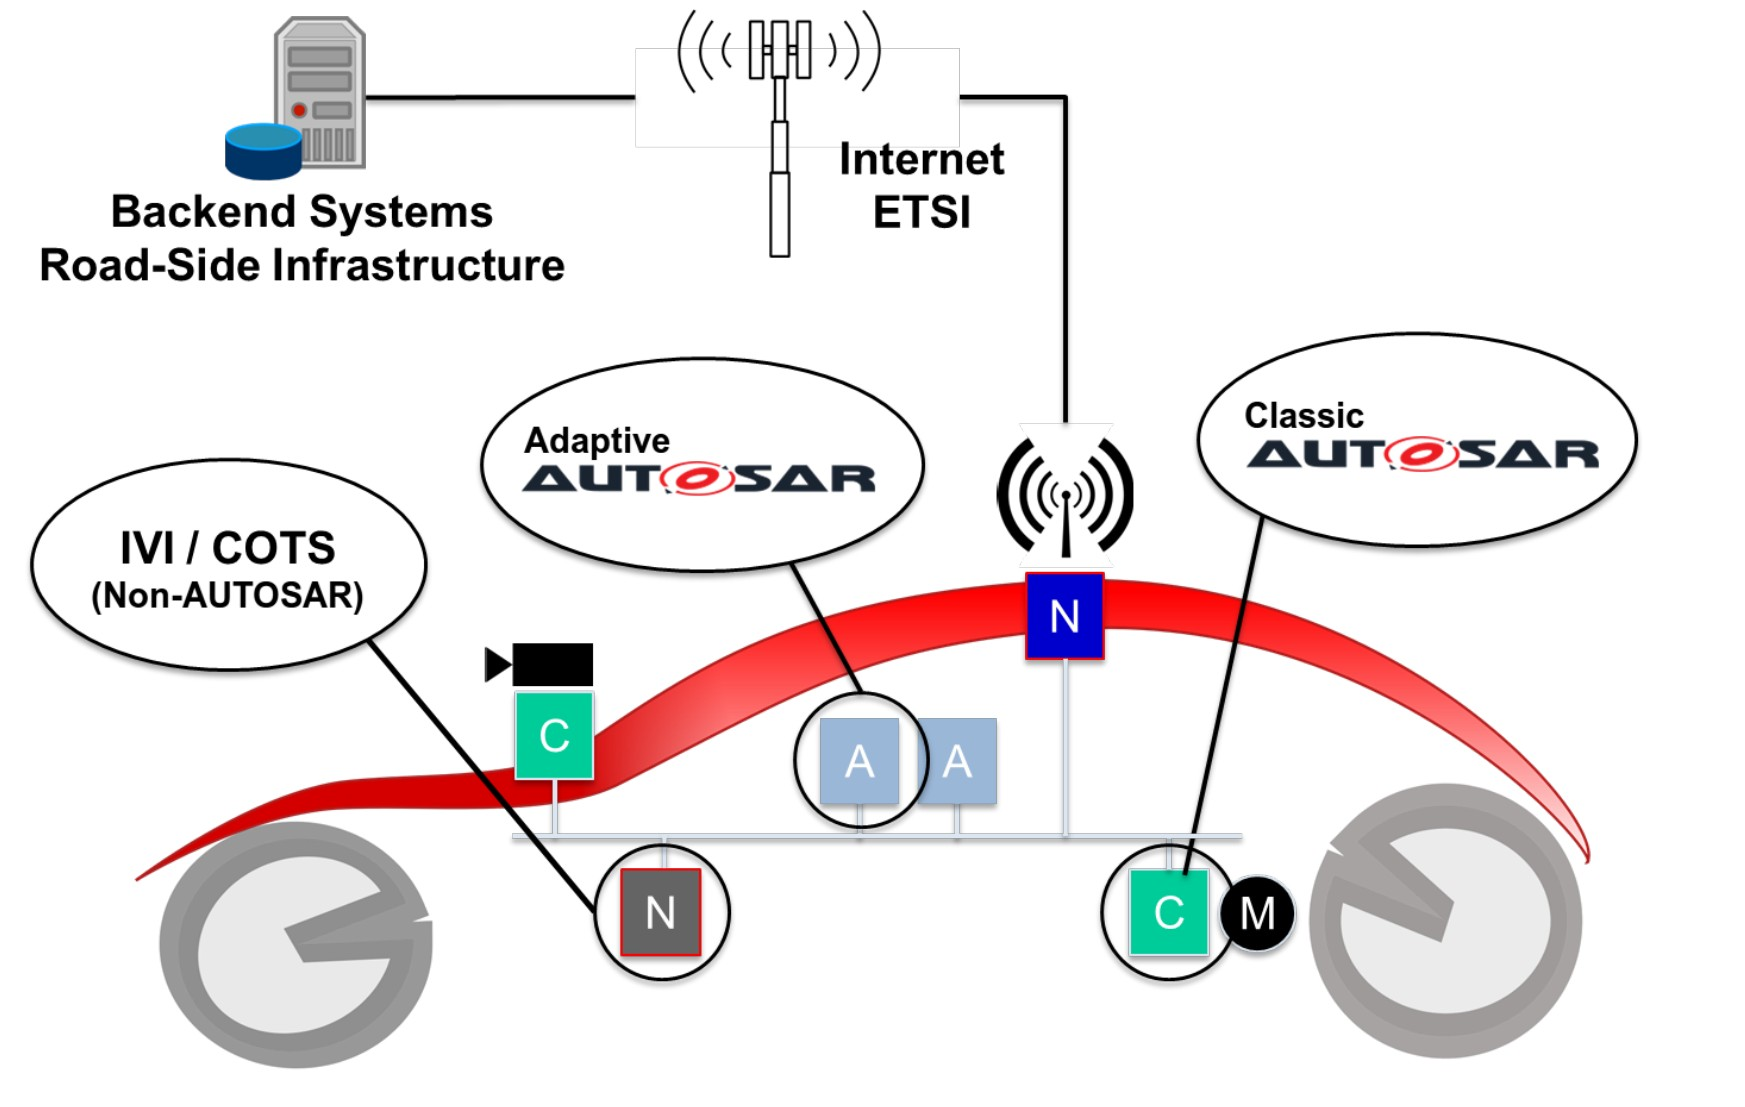
\includegraphics[width=1\textwidth]{Images/chapter2/ARandAP.jpg}
    \vspace{0.5cm}
    \caption{Exemplary deployment of different platforms \cite{autosar_platform_design}}
    \label{fig:autosar_adaptive_and_classic}
\end{figure}


The architectural designs of the Application Layer in the Adaptive Platform are based on a Service-Oriented Architecture (SOA). This allows the application to offer services to other applications and to subscribe to services provided by others. The Adaptive Platform provides a runtime environment known as the AUTOSAR Runtime for Adaptive Applications (ARA). ARA consists of a set of Functional Clusters that offer standardized services to the Adaptive Applications (AA) through a defined API.

These Functional Clusters are grouped into "Foundation" and "Services". The Foundation mainly provides platform-level functionalities such as Execution Management and Communication Management, while Services offer standard application-level capabilities. The platform runs on top of a POSIX-compliant operating system (e.g., Linux), which allows for high performance and flexibility. This layered architecture is depicted in Figure \ref{fig:autosar_adaptive_arch}, illustrating the separation between the Application, the Runtime Environment, and the underlying Operating System and Hardware.

\begin{figure}[h]
    \centering
    \includegraphics[width=1\textwidth]{Images/chapter2/AP_Arch.png}
    \vspace{0.5cm}
    \caption{Logical View of AUTOSAR Adaptive Platform Architecture \cite{autosar_platform_design}}
    \label{fig:autosar_adaptive_arch}
\end{figure}

\newpage

In the context of this project, the Adaptive Platform serves as the underlying framework for the Traffic Light Recognition System. This system utilizes the Scalable service-Oriented MiddlewarE over IP (SOME/IP) protocol and Data Distribution Service (DDS) to facilitate inter-process communication. The current implementation phase prioritizes the mechanisms of process interaction and system observability; consequently, the primary focus is placed on the Execution Management (ara::exm), Communication Management (ara::com), and Log and Trace (ara::log) functional clusters.


% \subsection{Scalable service-Oriented Middleware over IP (SOME/IP) Protocol}
% \label{sec:someip_protocol}
% \subsubsection{Service Definition}

% The Scalable service-Oriented Middleware over IP (SOME/IP) is an automotive middleware solution designed to enable efficient inter-process communication using a service-oriented architecture. Constructed on top of the Internet Protocol (IP), SOME/IP facilitates the dynamic deployment of applications by abstracting communication into defined services. A service within the SOME/IP protocol is formally defined as a logical grouping of zero or more remote procedure calls, data updates, and status properties, which are technically categorized as Methods, Events, and Fields.

% Methods represent the fundamental remote procedure calls (RPC) of the protocol. A method allows a client application (subscriber) to issue a call that is executed on the server side (provider). SOME/IP supports two primary types of methods: a "Request/Response" method, where the client waits for a reply containing the result or an error, and a "Fire \& Forget" method, where the client issues a command without expecting a response\cite[pp.~4, 15]{autosar_someip}. Events, in contrast, are specialized callback mechanisms used for data transport. They are unidirectional messages transmitted from the provider to the subscriber, typically triggered cyclically or upon a value change within the provider\cite[pp.~4, 16]{autosar_someip}.

% Fields serve to represent the status or property of a service instance. A Field is essentially a combination of up to three distinct access mechanisms: a Notifier, a Getter, and a Setter. The Notifier behaves similarly to an Event, transmitting the field's value to subscribers whenever it changes. The Getter is a method that allows a subscriber to explicitly query the current value of the field from the provider. Conversely, the Setter is a method that permits a subscriber to modify the value of the field on the provider side\cite[pp.~2, 4]{autosar_someip}. These interaction patterns form the basis of the SOME/IP communication model and are essential for automotive signal handling.

% \subsubsection{Motivation}

% The transition to Ethernet-based architectures in modern vehicles is driven by the demand for high-bandwidth applications, such as advanced infotainment and driver assistance systems. However, unlike traditional shared automotive buses (e.g., CAN), Ethernet is a switched network. This created a critical need for middleware capable of efficiently managing control data across this new medium.

% When the industry evaluated existing IT middleware standards—such as CORBA and Apache Thrift—they proved unsuitable. They were primarily designed for IT environments, lacked essential features like UDP support, and were too resource-intensive for the strict constraints of embedded Electronic Control Units (ECUs).

% To address this gap, Scalable service-Oriented Middleware over IP (SOME/IP) was developed. It provides an optimized protocol that supports CAN-like communication over Ethernet while seamlessly aligning with critical AUTOSAR concepts, such as the Client/Server and Sender/Receiver models. By fulfilling these specific automotive requirements, SOME/IP serves as the essential bridge connecting the IT/Linux domain with the Embedded/AUTOSAR domain within the vehicle network.

% % The transition toward Ethernet-based architectures in modern vehicles is driven by the increasing demand for high-bandwidth applications, such as advanced infotainment systems, driver assistance features like surround-view cameras, and the necessity for a high-speed domain backbone. While Ethernet provides a robust physical layer and the TCP/IP stack offers a proven solution for data transport, the automotive industry faced a significant challenge in identifying a suitable middleware solution capable of handling control data efficiently over this switched medium. Unlike traditional automotive buses, Ethernet is not a shared bus, necessitating a middleware that could efficiently manage unicast communication while keeping multicast and broadcast traffic to acceptable levels.

% % The primary motivation for developing Scalable service-Oriented Middleware over IP (SOME/IP) stemmed from the specific requirements of automotive communication that existing IT standards could not meet. The industry required a solution that supported CAN-like communication and MOST-like control messages but was optimized for switched Ethernet networks. An extensive evaluation of existing middleware solutions—including DCE RPC, CORBA, and Apache Thrift—revealed that these protocols were primarily designed for IT environments and were unsuitable for embedded automotive applications. These existing solutions often lacked necessary features (such as UDP support), were too resource-intensive, or required significant modification and "stripping down" to function within the constraints of automotive electronic control units (ECUs).

% % Furthermore, compatibility with the AUTOSAR standard was a critical factor in the development of SOME/IP. Existing IT solutions did not support AUTOSAR, and integrating them would have been critical and difficult to standardize. The industry needed a protocol that aligned with AUTOSAR concepts, such as the Client/Server model (Request/Response) and the Sender/Receiver model (Fire and Forget), without being restricted by the AUTOSAR license itself. SOME/IP was designed to fill this specific gap, serving as the only solution that satisfies all automotive requirements while acting as a bridge between the IT/Linux domain and the Embedded/AUTOSAR domain. Consequently, SOME/IP provides a scalable, efficient middleware solution that ensures header layouts and communication behaviors are optimized for the vehicle network.


% \subsubsection{Protocol Objectives and Architectural Role}

% \gls{SOMEIP} acts as a fundamental automotive middleware solution designed to facilitate efficient inter-process communication within the vehicle network. It provides a comprehensive specification for \glspl{RPC}, event notifications, and the underlying serialization wire format.. While initially developed to address the limitations of enterprise middleware in automotive environments, its primary architectural role today is to ensure scalability and resource efficiency across heterogeneous systems.

% A core objective of the protocol is to operate across a diverse range of hardware platforms. It scales seamlessly from small, resource-constrained electronic control units (ECUs) like cameras to complex, high-performance infotainment head units. To achieve this, the serialization protocol is designed to be linearly serialized without complex dynamic operations, ensuring it can be supported by simple tooling and run efficiently on embedded devices.

% From an architectural perspective, \gls{SOMEIP} embodies the principles of \gls{SOA} by abstracting underlying network complexity. By exposing well-defined Service Interfaces rather than raw signals, it promotes loose coupling between components. This is enforced by the \gls{SOMEIP} Service Discovery (SD) mechanism, which allows clients to dynamically detect available service instances at runtime. This shift enables the modularization of complex distributed applications, facilitating a flexible and robust vehicle network backbone that bridges the IT-centric Linux domain and the embedded \gls{AUTOSAR} domain.

% \subsubsection{Specification of \gls{SOMEIP} Message Format (Serialization)}

% The specification of \gls{SOMEIP} message format defines how communication data is structured, serialized, and transmitted between distributed components in an automotive Ethernet environment. At its core, a \gls{SOMEIP} message consists of a well-defined header followed by a payload. The header carries metadata crucial for message identification, routing, version control, and error handling, while the payload contains application-level data encoded according to strict serialization rules. These rules support a variety of data types and ensure consistency, extensibility, and backward compatibility across different versions of software and \glspl{ECU}. By standardizing both the header and payload structures, \gls{SOMEIP} enables reliable and scalable service-oriented communication in modern vehicle architectures.

% In this figure, the structure of \gls{SOMEIP} consists of two major components: \textbf{Header} and \textbf{Payload}.

% \begin{figure}[h]
%     \centering
%     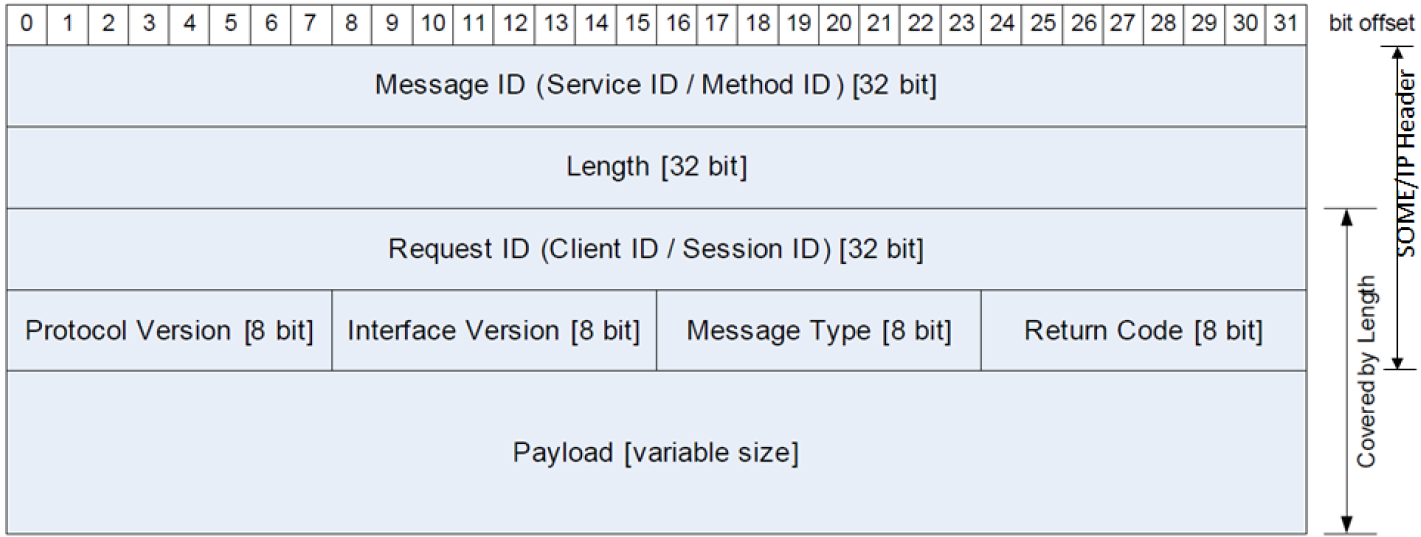
\includegraphics[width=1\textwidth]{Images/chapter2/HeaderSomeip.png}
%     \vspace{0.5cm}
%     \caption{Structure of \gls{SOMEIP} message format}
%     \label{fig:someip_structure}
% \end{figure}

% \paragraph*{Header of \gls{SOMEIP} protocol:} The header of the \gls{SOMEIP} protocol includes essential fields such as the \textbf{Message ID}, \textbf{Length}, \textbf{Client ID}, \textbf{Session ID}, \textbf{Protocol Version}, \textbf{Interface Version}, \textbf{Message Type}, and \textbf{Return Code}. These fields provide necessary metadata for identifying services, ensuring compatibility, managing sessions, and indicating the message status during communication between \glspl{ECU}.

% \textbf{Message ID [32 Bit]:} The Message ID is a 32-bit identifier used to uniquely identify either a remote procedure call (RPC) method or an event within the \gls{SOMEIP} protocol. This identifier is structured into two parts: the upper 16 bits represent the \textbf{\textit{Service ID}}, which distinguishes up to 65,536 different services, and the lower 16 bits represent the \textbf{\textit{Method ID}}, which specifies individual methods or events within that service. By convention, Method IDs in the range from \texttt{0x0000} to \texttt{0x7FFF} are reserved for RPC methods, while IDs in the range from \texttt{0x8000} to \texttt{0x8FFF} are used for events and notifications. This structured format ensures clear and scalable message identification across the entire system.

% \textbf{Length [32 Bit]:} Length field will show the length in Byte starting from Request ID/Client ID until the end of the SOME/IP message.

% \textbf{Request ID [32 Bit]}: The Request ID is a 32-bit field used to uniquely distinguish concurrent service calls between clients and servers in \gls{SOMEIP}. It is logically divided into two 16-bit segments: the \textbf{\textit{Client ID}} and the \textbf{\textit{Session ID}}. The Client ID identifies the sender of the request, allowing the receiver to differentiate among multiple clients. The Session ID is used to distinguish multiple invocations of the same method, enabling parallel or sequential tracking of communication flows. The Request ID must remain unique during the lifetime of a request-response transaction to ensure proper matching of replies.

% In some implementations, especially in large systems like a vehicle-wide network, the Request ID may be further structured to enhance uniqueness and traceability. In this extended form, the Request ID is split into three components: an 8-bit \textbf{\textit{Client ID Prefix}} (e.g., a diagnostic address or preconfigured application ID), an 8-bit \textbf{\textit{Client ID}}, and a 16-bit \textbf{\textit{Session ID}}. This structure supports globally unique identification across all \glspl{ECU} in the vehicle and facilitates more flexible configuration and routing of service calls.

% \textbf{Protocol Version [8 Bit]}: This field indicates the version of the \gls{SOMEIP} protocol used in the message. It allows systems to detect and handle incompatible changes in the protocol format. The Protocol Version only reflects the versioning of the header structure, not the payload. Currently, the standard value for this field is \texttt{0x01}. Any incompatible change in the header layout must result in an increment of this version to maintain interoperability between different protocol versions.

% \textbf{Interface Version [8 Bit]}: The Interface Version identifies the major version of the service interface and reflects changes in the structure of the payload data. A receiver uses this value to determine whether it can correctly interpret the message contents. Unlike the protocol version, which is about the header, the interface version focuses on the application-layer data structures and semantics. This field is particularly important when evolving service definitions across software updates.

% \textbf{Message Type [8 Bit]}: The Message Type field defines the nature of the message being transmitted. It specifies whether the message is a request, response, notification, or an error. This is a table shows type of message, each message corresponds to number of code 

% \textbf{Return Code [8 Bit]}: The Return Code is used to indicate the status of message processing. While it is generally set to \texttt{0x00} (E\_OK) in non-response messages, it conveys success or failure in response and error messages. For example, \texttt{0x01} indicates a generic error, \texttt{0x03} signals an unknown method, and \texttt{0x09} is used for malformed messages. This field provides a mechanism for reporting both application-level and protocol-level issues in communication.

% \newpage
% \begin{figure}[h]
%     \centering
%     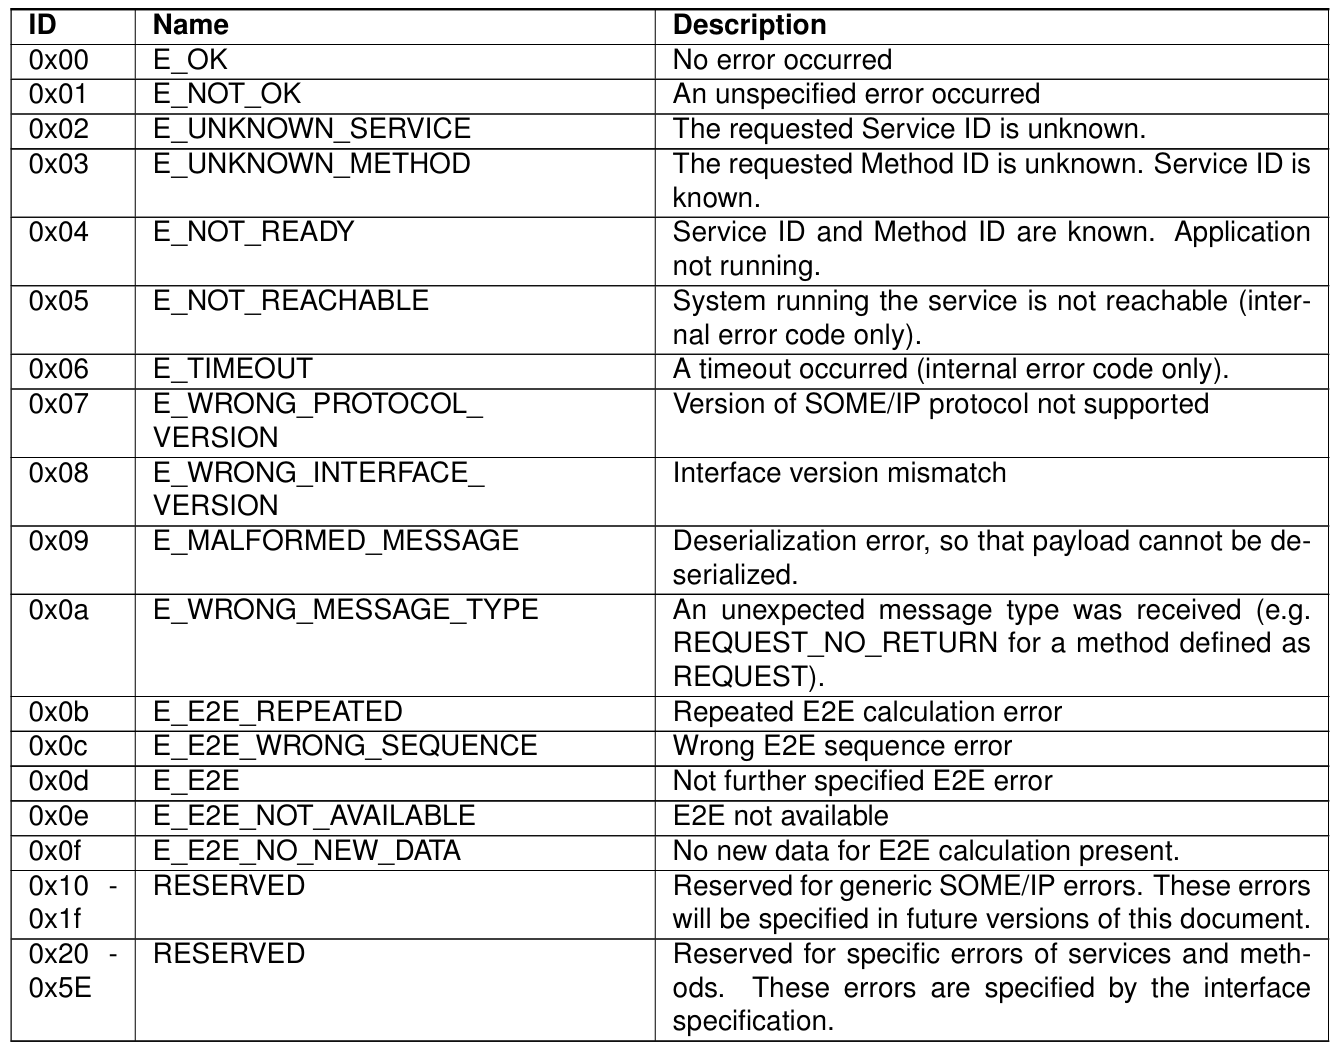
\includegraphics[width=1\textwidth]{Images/chapter2/errSomeip.png}
%     \vspace{0.5cm}
%     \caption{The table of Message Type field}
% \end{figure}
% \newpage
% \paragraph*{Payload and Serialization:}
% The \textbf{Payload} in a \gls{SOMEIP} message carries the actual data that is exchanged between a client and a server. It represents the parameters for a method call, the return values of a response, or the content of a notification/event. The payload structure is determined by the service interface definition and may consist of basic data types (e.g., integers, booleans, floats) or complex data types such as structs, arrays, strings, unions, and enumerations. Depending on the message context, the payload may be empty or contain multiple serialized arguments.

% \textbf{Serialization} refers to the process of encoding these data structures into a linear byte stream suitable for transmission over the network. The SOME/IP protocol specifies strict rules for serialization, including byte ordering (typically big-endian for header fields), memory alignment, and padding strategies. For complex types like structs, serialization closely follows in-memory layout with explicit handling of optional members and extensibility using data IDs and tags. Arrays and strings can be fixed or variable in length and often include a length field to aid deserialization. These rules ensure interoperability between different ECUs, allowing them to parse and understand messages even when optional fields or future extensions are added.

% \begin{figure}[h]
%     \centering
%     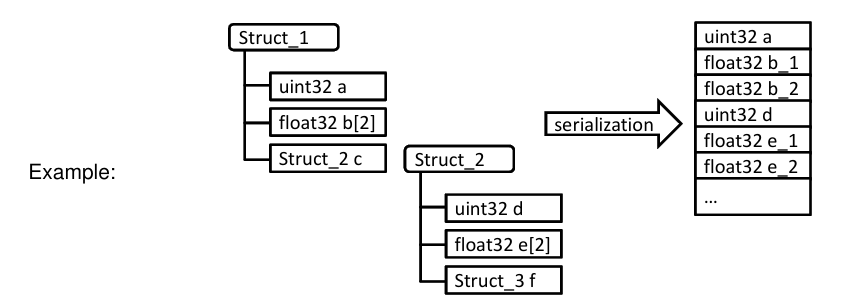
\includegraphics[width=1\textwidth]{Images/chapter2/serializationSomeip.png}
%     \vspace{0.5cm}
%     \caption{The mechanism of serialization code structure}
% \end{figure}


% Furthermore, SOME/IP supports flexible and forward-compatible serialization mechanisms through the use of tag-length-value (TLV) encoding. TLV allows new members to be added at arbitrary positions in a message, enhancing compatibility between software versions. During deserialization, unknown tags can be skipped, which prevents older receivers from crashing due to unexpected data. This extensibility is crucial in automotive systems where long product lifecycles and incremental software updates are common. This is an example of serialization of the structure code with tags.

% \newpage

% \begin{figure}[h]
%     \centering
%     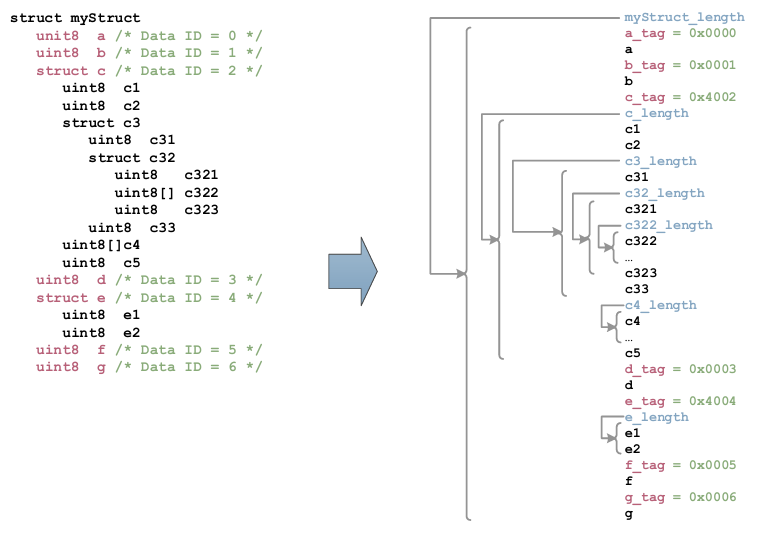
\includegraphics[width=1\textwidth]{Images/chapter2/serializationexSomeip.png}
%     \vspace{0.5cm}
%     \caption{An example of serialization of the structure code with tags}
% \end{figure}

% To sum up, the specification of the \gls{SOMEIP} message format provides a robust framework for structuring and transmitting data across distributed systems within automotive networks. By clearly defining the header fields and enforcing rigorous serialization rules for the payload, \gls{SOMEIP} ensures message consistency, interoperability, and forward compatibility. Whether handling simple method calls or complex data structures, the protocol's design supports scalable and efficient communication between heterogeneous \glspl{ECU}. This serialization standard is a key in enabling service-oriented architectures for connected and software-defined vehicles, paving the way for reliable in-vehicle communication and future-proof software integration.

% \subsubsection{Specification of \gls{SOMEIP} Protocols}

% The \gls{SOMEIP} protocol facilitates service-oriented communication through three core interaction mechanisms: \textbf{Methods}, \textbf{Events}, and \textbf{Fields}. These elements define how data and commands are exchanged between clients and servers, supporting various communication patterns ranging from synchronous remote procedure calls to asynchronous state synchronization.

% \paragraph*{Methods:}
% Methods allow a client to invoke a procedure on a server instance. \gls{SOMEIP} distinguishes between two primary types of method invocations based on whether a reply is required:

% \begin{figure}[h]
%     \centering
%     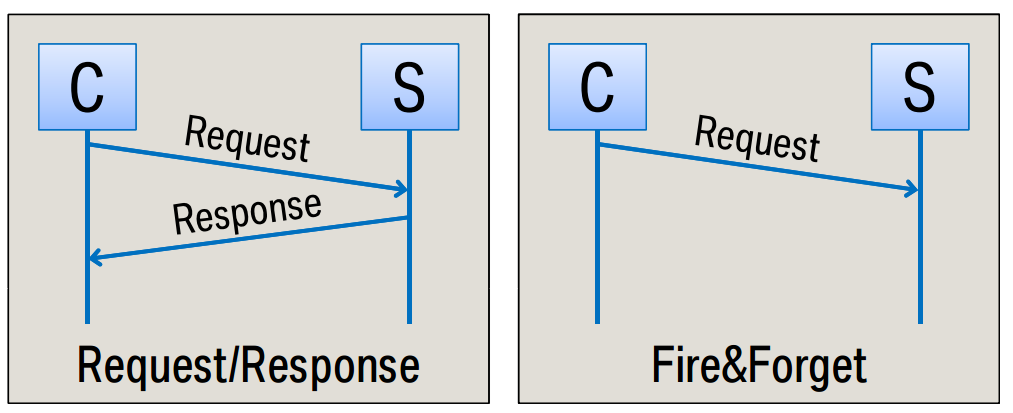
\includegraphics[width=0.8\textwidth]{Images/chapter2/MethodSomeip.png}
%     \vspace{0.5cm}
%     \caption{Methods in \gls{SOMEIP} \cite{open_alliance_someip}}
% \end{figure}

% \newpage
% \textbf{Request/Response:} This is the standard Remote Procedure Call (RPC) pattern. The client sends a \texttt{REQUEST} message (type \texttt{0x00}) and waits for a feedback. The server processes the command and returns either a \texttt{RESPONSE} message (type \texttt{0x80}) containing the result or an \texttt{ERROR} message (type \texttt{0x81}) if the operation failed. This pattern ensures transactional integrity and is equivalent to synchronous service calls in 

% \textbf{Fire \& Forget:} In this pattern, the client sends a \texttt{REQUEST\_NO\_RETURN} message (type \texttt{0x01}). The server executes the method but does not send a response, regardless of success or failure. This is useful for non-critical commands where bandwidth optimization is prioritized over confirmation, effectively decoupling the client from the server's processing time.

% \paragraph*{Events:}
% An Event represents a unidirectional, asynchronous data transmission from the server to subscribed clients. It utilizes the \texttt{NOTIFICATION} message type (\texttt{0x02}).

% Events follow the Publish/Subscribe model. A client must explicitly subscribe to an event group to receive these messages. The server triggers events based on specific logic:

% \begin{figure}[h]
%     \centering
%     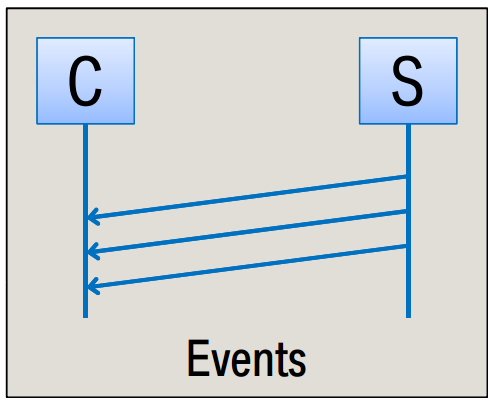
\includegraphics[width=0.4\textwidth]{Images/chapter2/EventSomeip.png}
%     \vspace{0.5cm}
%     \caption{Events in \gls{SOMEIP} \cite{open_alliance_someip}}
% \end{figure}

% \textbf{Cyclic:} Transmitted at a fixed time interval (e.g., vehicle speed sent every 100ms).

% \textbf{On Change:} Transmitted only when the value changes (e.g., a door open warning).

% \paragraph*{Fields:}
% A Field represents a status or a state variable managed by the server. Unlike a simple Event, a Field combines three distinct access mechanisms to ensure data consistency across the distributed system:

% \begin{figure}[h]
%     \centering
%     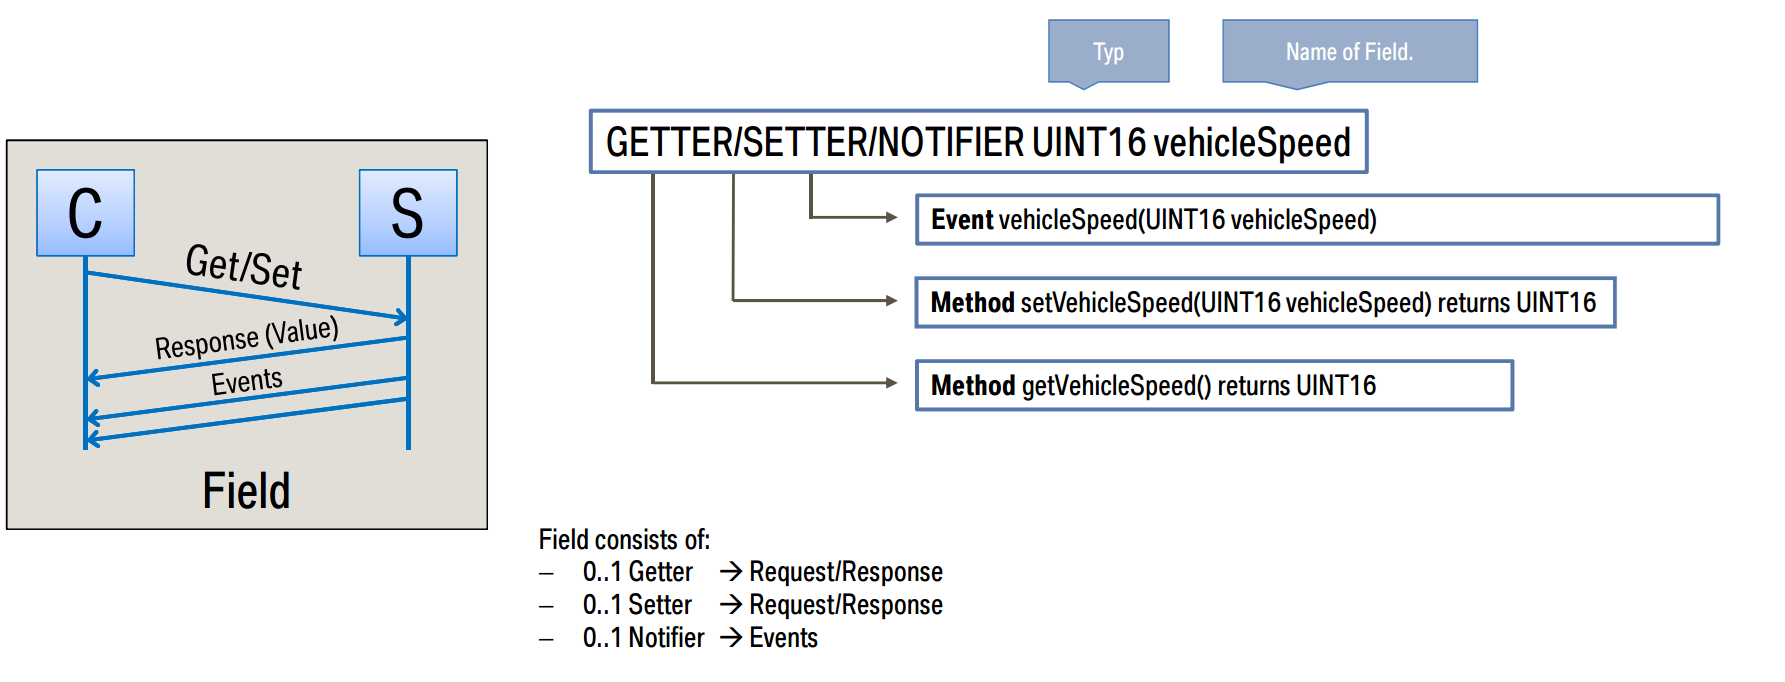
\includegraphics[width=1\textwidth]{Images/chapter2/FieldSomeip.png}
%     \vspace{0.5cm}
%     \caption{Fields in \gls{SOMEIP} \cite{open_alliance_someip}}
% \end{figure}

% \textbf{Setter:} A Request/Response method allowing a client to modify the value of the field remotely.

% \textbf{Getter:} A Request/Response method allowing a client to explicitly read the current value of the field.

% \textbf{Notifier:} An asynchronous event notification sent to subscribers whenever the field's value changes.

% \paragraph*{Comparison: Event vs. Field:}
% While both Events and Field Notifiers use asynchronous notifications to transmit data, their architectural purpose differs regarding state management:

% \textbf{Events} are best suited for momentary occurrences or streaming data where the history is less relevant than the immediate update. If a client subscribes to an Event after a transmission has occurred, it must wait for the next occurrence to receive data.

% \textbf{Fields} represent a persistent state. The inclusion of \textbf{Getter} and \textbf{Setter} methods ensures that a client can retrieve the current state immediately upon connecting, without waiting for the next change notification. Therefore, Fields are preferred when data synchronization and initial state validity are critical.

% Fields support both pull-based (getter/setter) and push-based (notifier) communication styles. This concept can be mapped to shared variables or observable state in enterprise software where consistent data synchronization is required.

% \paragraph*{Error Handling:}

% In addition to the three communication elements, \gls{SOMEIP} provides a robust error handling mechanism. Every message includes a \texttt{Return Code} field that indicates whether the operation succeeded (\texttt{0x00} for E\_OK) or failed (e.g., \texttt{0x03} for E\_UNKNOWN\_METHOD).

% When additional diagnostic information is needed, servers can send a dedicated \texttt{ERROR} message (\texttt{0x81}), which may include structured error payloads such as exception types or debug messages. This supports fault detection, debugging, and graceful degradation—critical concerns in enterprise-grade software systems.

% Moreover, protocol-level validations such as version mismatch detection, unexpected message checks, and session management are built-in, ensuring communication resilience and system integrity.

% \newpage
% \begin{figure}[h]
%     \centering
%     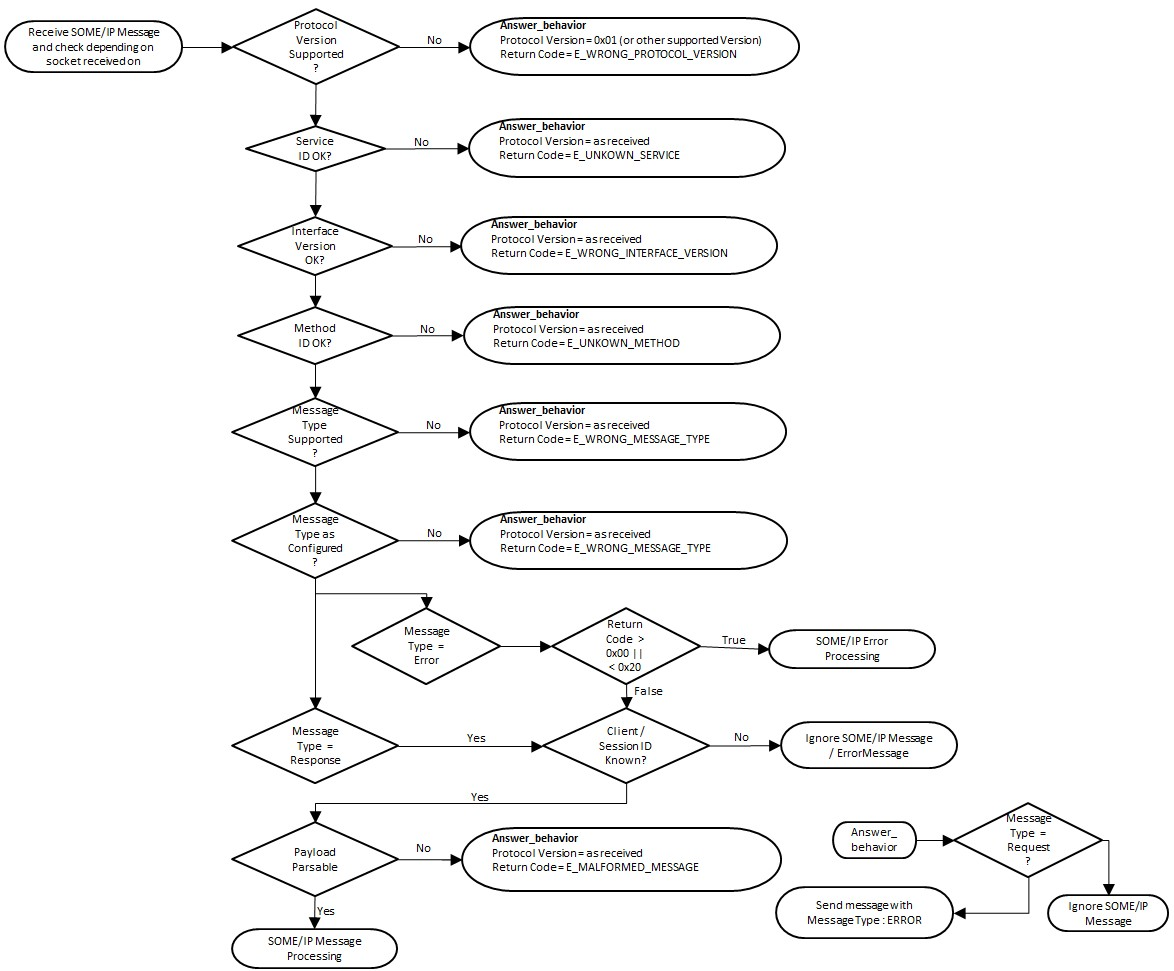
\includegraphics[width=1\textwidth]{Images/chapter2/ErrorHandlerSomeip.jpg}
%     \vspace{0.5cm}
%     \caption{Error handling in \gls{SOMEIP} \cite{open_alliance_someip}}
% \end{figure}


% The specification of \gls{SOMEIP} communication through its Method, Event, and Field elements, along with a comprehensive error handling strategy, demonstrates a well-structured approach to designing scalable and interoperable distributed systems. These mechanisms are not only tailored to meet the stringent real-time and safety requirements of automotive applications, but they also reflect well practices found in enterprise software architecture, such as modularity, service encapsulation, event-driven design, and fault tolerance. Understanding and applying these communication models facilitates the development of robust service-oriented systems that align with modern software engineering principles.

% \subsubsection{SOME/IP-SD (SOME/IP Service Discovery)}

% SOME/IP Service Discovery (SOME/IP-SD) is the dedicated protocol extension used to manage the availability of service instances and the dynamic establishment of communication paths within an automotive Ethernet network. While standard IT service discovery mechanisms focus primarily on locating a service, SOME/IP-SD is optimized for automotive requirements, focusing heavily on service availability (determining if a service is ready to be used) and the management of Publish/Subscribe relationships for event handling. The protocol is designed to run on embedded devices with limited overhead, allowing multiple service interactions to be encoded within a single packet. SOME/IP-SD messages are transported over UDP (and less commonly TCP) using the standard SOME/IP header, but they utilize a fixed Message ID of 0xFFFF 8100 to distinguish them from standard application RPC messages.
% The architecture of a SOME/IP-SD message consists of a specific payload layout that follows the standard SOME/IP header. This payload is organized into Flags, an Entries Array, and an Options Array. The Entries Array contains the core commands, such as finding services or subscribing to events, while the Options Array carries variable data, such as IP addresses, port numbers, or configuration strings, which are referenced by the entries using indices. A vital component of the SD header is the Flag field, specifically the Reboot Flag. This flag allows ECUs to detect if a communication partner has restarted. The Session ID in the header increments with every transmission; if a receiver detects that the Session ID has reset or that the Reboot Flag has been toggled, it knows the partner ECU has rebooted and can re-initialize subscriptions or discard stale state data.

% \begin{figure}[h]
%     \centering
%     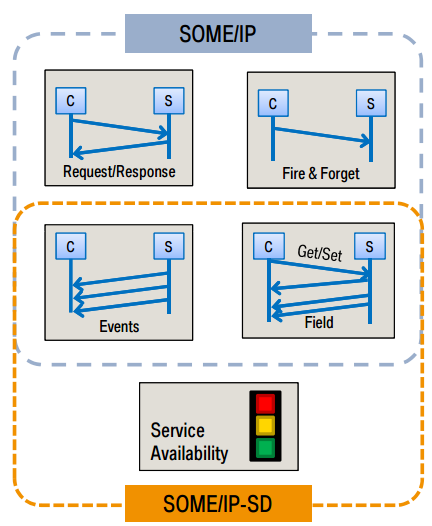
\includegraphics[width=0.5\linewidth]{Images//chapter2/someip_sd.png}
%     \vspace{0.5cm}
%     \caption{SOME/IP Service Discovery \cite{open_alliance_someip}}
%     \label{fig:someip_sd}
% \end{figure}

% \paragraph{Service Discovery Mechanisms:} There are 2 Service Discovery Mechanism: 

% \textbf{Offer and Find:} The primary function of SOME/IP-SD is to match Clients (service consumers) with Servers (service providers). The protocol utilizes specific entry types to achieve this: \texttt{OfferService} and \texttt{FindService}. When a Server ECU starts up and a service instance becomes available, it enters an "Initial Wait Phase" followed by a "Repetition Phase," where it broadcasts \texttt{OfferService} entries (typically via Multicast) to announce its presence to the network. If a Client ECU requires a service that it has not yet seen offered, it sends a FindService entry. Upon receiving a Find message, the Server responds with a unicast \texttt{OfferService} to inform the specific Client that the service is available. These entries contain a Time-To-Live (TTL) field; a non-zero TTL indicates the service is valid for a specific duration (e.g., 3 seconds), whereas a TTL of zero represents a \texttt{StopOfferService} message, informing the network that the service is no longer available.

% \begin{figure}[h]
%     \centering
%     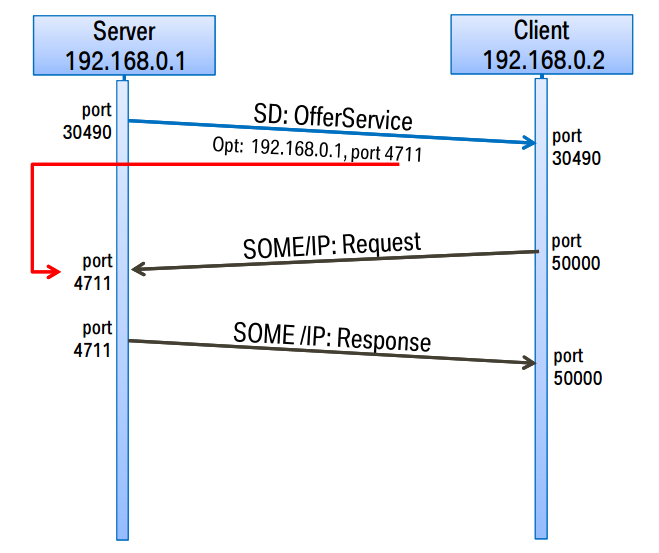
\includegraphics[width=0.5\linewidth]{Images//chapter2/someip_sd_offerandfind.png}
%     \vspace{0.5cm}
%     \caption{SOME/IP-SD Offer and Find Mechanism \cite{open_alliance_someip}}
%     \label{fig:someip-sd/findoffer}
% \end{figure}
% \newpage
% \textbf{Publish/Subscribe Management:} Beyond simple discovery, SOME/IP-SD manages the dynamic routing of events through a Publish/Subscribe mechanism. This ensures that the network is not flooded with event messages unless a Client explicitly requires them. This is handled through specific entry types: SubscribeEventgroup and SubscribeEventgroupAck. When a Client determines a service is available (via an \texttt{OfferService}), it sends a \texttt{SubscribeEventgroup} entry to the Server to request specific data streams. The Server validates this request and responds with a \texttt{SubscribeEventgroupAck} (Acknowledgement) if successful, or a \texttt{SubscribeEventgroupNack} (Negative Acknowledgement) if the request fails. Only after this handshake does the Server begin transmitting the actual event data via standard SOME/IP notification messages. 

% \begin{figure}[h]
%     \centering
%     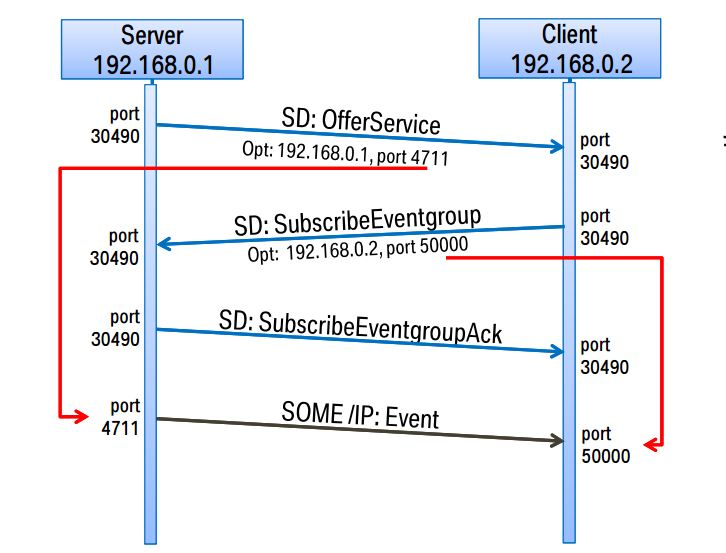
\includegraphics[width=0.5\linewidth]{Images//chapter2/someip_sdpubsub.png}
%     \vspace{0.5cm}
%     \caption{SOME/IP-SD Publish/Subscribe Mechanism \cite{open_alliance_someip}}
%     \label{fig:enter-label/pubsub}
% \end{figure}

% To link the abstract discovery of a service to the physical network parameters required to connect to it, SOME/IP-SD uses Endpoint Options. An SD Entry (like an Offer or Subscribe) does not contain the IP address or port itself; instead, it points to an Option in the Options Array. For example, an IPv4 Endpoint Option contains the IP address, the transport protocol (UDP or TCP), and the Port Number where the service can be reached. For multicast events, a Multicast Option is used by the Server in the \texttt{SubscribeEventgroupAck} to tell the Client which Multicast IP and Port to listen to for incoming events. This separation allows for efficient packing, where multiple entries can share the same endpoint options within a single message.

% \begin{figure}[h]
%     \centering
%     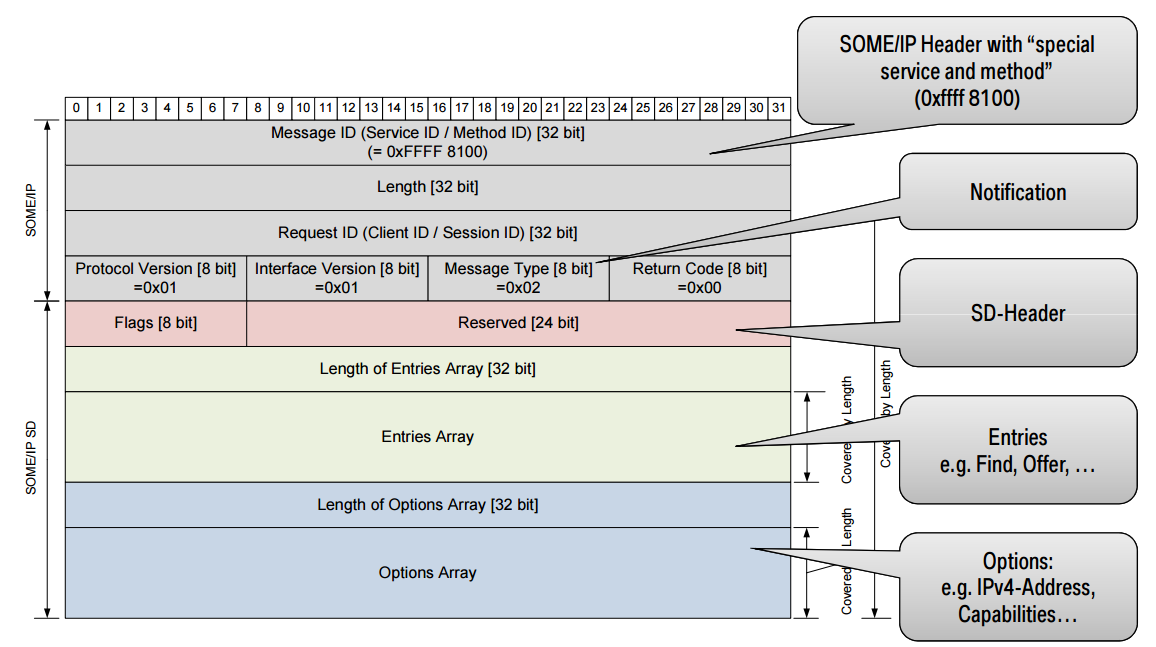
\includegraphics[width=1\linewidth]{Images//chapter2/someip_sdheader.png}
%     \vspace{0.5cm}
%     \caption{SOMEIP/SD Header \cite{open_alliance_someip}}
%     \label{fig:Someip-sdheader}
% \end{figure}
% \newpage
% \subsubsection{SOME/IP Transport Layer Bindings}

% The SOME/IP protocol is designed to operate independently of the underlying transport layer, primarily utilizing User Datagram Protocol (UDP) and Transmission Control Protocol (TCP) to transmit messages over IP-based automotive networks. The selection of the specific transport protocol is critical as it dictates the reliability, latency, and payload capacity of the communication. While UDP offers a lightweight, connectionless model suitable for frequent, small messages, TCP provides a robust, connection-oriented channel for larger data streams. Additionally, to bridge the gap between the limitations of UDP and the need to transport large data packets without the overhead of TCP, the SOME/IP Transport Protocol (SOME/IP-TP) was developed to allow for segmentation over UDP.

% \textbf{UDP Binding (User Datagram Protocol)}

% The UDP binding is the most fundamental mode of transport for SOME/IP, achieved by encapsulating SOME/IP messages directly within UDP packets. It is a connectionless protocol, meaning no handshake is required before data transmission begins. A client and server typically use a single unicast UDP connection for all methods and events configured for UDP communication, and a separate multicast connection for multicast events. Due to the nature of UDP and the standard Maximum Transmission Unit (MTU) of Ethernet frames, the payload of a SOME/IP message transmitted via UDP is strictly limited to between 0 and 1400 bytes to prevent IP fragmentation and ensure protocol stability.

% UDP is the preferred choice for automotive applications requiring very low latency (typically under 100ms) and fast reaction times. It is ideal for "Fire \& Forget" communication or cyclic data transmission—such as vehicle speed or engine RPM—where the occasional loss of a packet is acceptable because the next cycle will update the information shortly. The protocol supports "Maybe" reliability semantics, meaning the application must be designed to handle scenarios where a message might not reach its destination. Furthermore, UDP is the required transport mechanism for multicast communication, where a single publisher sends notifications to multiple subscribers simultaneously .

% The primary drawback of the standard UDP binding is the strict payload limitation; it cannot natively transport messages larger than 1400 bytes. Additionally, because it lacks the robustness features of TCP, it does not guarantee delivery, order, or protection against duplication. If a packet is lost in the network, it is not automatically retransmitted by the transport layer, forcing the application layer to handle error scenarios or timeouts.


% \textbf{TCP Binding (Transmission Control Protocol)}

% The TCP binding provides a reliable, connection-oriented channel for SOME/IP messages. Unlike UDP, TCP supports the segmentation of payloads, allowing for significantly larger SOME/IP messages that far exceed the 1400-byte limit of UDP. The connection is managed actively: the client is responsible for opening the TCP connection when the first method call or notification is required and must re-establish it if it fails. To mitigate latency issues often associated with TCP, the protocol specification recommends disabling Nagle’s algorithm (\texttt{TCP\_NODELAY}). To assist testing tools in identifying message boundaries within the continuous TCP stream, "Magic Cookie" messages may be inserted into the stream at regular intervals.

% TCP is utilized when "Exactly Once" reliability is required, ensuring that messages arrive correctly, in order, and without duplication. It is the optimal choice for transmitting large chunks of data—such as map data, diagnostic logs, or complex data structures—where the payload exceeds 1400 bytes and the strict latency requirements of control loops are not the primary constraint.

% The robustness of TCP comes at the cost of higher overhead and latency compared to UDP. The management of the connection adds complexity; the system must handle opening, closing, and monitoring the connection state. Furthermore, TCP does not support multicast; it is strictly a unicast, point-to-point protocol. If the server closes the connection unexpectedly, it can lead to synchronization issues where the client attempts to immediately re-establish the link.


% \textbf{SOME/IP-TP (Transport Protocol)}

% SOME/IP-TP is not a separate transport layer but a protocol extension applied on top of UDP to enable the segmentation of large messages that would otherwise require TCP. When a SOME/IP message is too large for a single UDP packet, it is split into smaller "segments". These segments utilize a specific Message Type (setting the TP-Flag to 1) and insert a TP-Header immediately after the standard SOME/IP header. This TP-Header contains an Offset field (indicating where in the original message the current segment belongs) and a More Segments Flag (indicating if more data follows). The receiver is responsible for collecting these segments and reassembling the original message based on the Request ID (Client ID and Session ID).

% The primary use case for SOME/IP-TP is transmitting large data payloads (>1400 bytes) in scenarios where the hard latency requirements prohibit the use of TCP. It allows engineers to maintain the speed and connectionless nature of UDP while bypassing its size limitations. It is often used for transmitting large sensor data or camera images where real-time delivery is prioritized over the absolute guarantee of delivery provided by TCP.

% SOME/IP-TP introduces significant complexity to the receiving stack. The receiver must manage reassembly buffers and handle various error cases, such as overlapping, duplicated, or missing segments. Crucially, SOME/IP-TP does not support the reordering of segments; if a segment is lost or arrives out of order in a way the buffer cannot handle, the entire assembly process for that message is canceled. Furthermore, the payload of all segments (except the last one) must be a multiple of 16 bytes to ensure alignment.


% \begin{table}[h!]
% \centering
% \renewcommand{\arraystretch}{1.5} % Adjusts row height for better readability
% \begin{tabularx}{\textwidth}{|l|X|X|X|}
% \hline
% \textbf{Feature} & \textbf{UDP Binding} & \textbf{TCP Binding} & \textbf{SOME/IP-TP} \\ \hline
% \textbf{Definition} & 
% User Datagram Protocol; a connectionless, lightweight transport protocol. & 
% Transmission Control Protocol; a connection-oriented, reliable protocol. & 
% Transport Protocol; a protocol extension applied on top of UDP to enable segmentation of large messages. \\ \hline
% \textbf{Payload Capacity} & 
% Strictly limited to 0--1400 bytes to avoid IP fragmentation. & 
% Supports large payloads (stream-based) significantly larger than 1400 bytes. & 
% Supports large payloads ($>1400$ bytes) by segmenting them into smaller packets fitting the MTU. \\ \hline
% \textbf{Reliability} & 
% ``Maybe'' reliability; messages might reach the partner, but loss, duplication, or reordering is handled by the application. & 
% ``Exactly Once'' reliability; handles packet loss, reordering, and duplication automatically. & 
% Dependent on UDP; strictly does not support reordering of segments. If a segment is missing, reassembly is canceled [8]. \\ \hline
% \textbf{Latency} & 
% Very low latency; suitable for requirements $<100$ms. & 
% Higher latency due to connection overhead and reliability mechanisms (retransmissions). & 
% Lower latency than TCP; designed for large data with hard latency requirements. \\ \hline
% \textbf{Connection Management} & 
% Connectionless; no handshake required. & 
% Active connection management required (Open/Close); Client initiates connection. & 
% Connectionless (rides on UDP); requires Session Handling (Session ID) to track segments. \\ \hline
% \textbf{Multicast Support} & 
% Supported; required for multicast events. & 
% Not supported; Unicast only. & 
% Supported (as it operates over UDP). \\ \hline
% \textbf{Primary Use-Case} & 
% Cyclic data (e.g., vehicle speed), small events, ``Fire \& Forget'' communication. & 
% Large data chunks (e.g., map data, diagnostics) where no hard latency limit exists. & 
% Large data transmission (e.g., sensor fusion data) where TCP latency is unacceptable. \\ \hline
% \end{tabularx}
% \caption{Comparison of SOME/IP Transport Layer Bindings}
% \label{tab:someip_transport_comparison}
% \end{table}


\subsection{Scalable service-Oriented Middleware over IP (SOME/IP) Protocol}
\label{sec:someip_protocol}

Scalable service-Oriented Middleware over IP (SOME/IP) is an automotive middleware protocol designed for service-oriented communication over Ethernet. It was introduced to support the transition from signal-based in-vehicle networks, such as CAN and LIN, toward IP-based communication required by modern infotainment, ADAS, and software-defined vehicle architectures. Unlike traditional bus communication, Ethernet is switched and packet-based; therefore, applications require middleware that can describe services, discover providers dynamically, serialize data consistently, and transport messages efficiently between distributed ECUs.

Within Adaptive AUTOSAR, SOME/IP is one of the communication bindings used by Communication Management (\texttt{ara::com}). Its main role is to expose application functionality through well-defined service interfaces rather than direct signal access. A SOME/IP service is composed of three main interaction elements: {Methods}, {Events}, and {Fields}. Methods implement remote procedure calls between a client and a provider. They can follow a request/response pattern, where the client waits for a result, or a fire-and-forget pattern, where no response is expected. Events implement unidirectional data transmission from a provider to subscribed clients, usually triggered cyclically or when a value changes. Fields represent service state and combine getter, setter, and notifier mechanisms, allowing clients to read, modify, or subscribe to state changes \cite{autosar_someip}.

\subsubsection{SOME/IP Message Format and Serialization}

A SOME/IP message consists of a fixed header followed by an application payload. The header contains the information required to identify the service, route the message, distinguish concurrent calls, verify compatibility, and report errors. Figure~\ref{fig:someip_structure} shows the general structure of a SOME/IP message.

\begin{figure}[h]
    \centering
    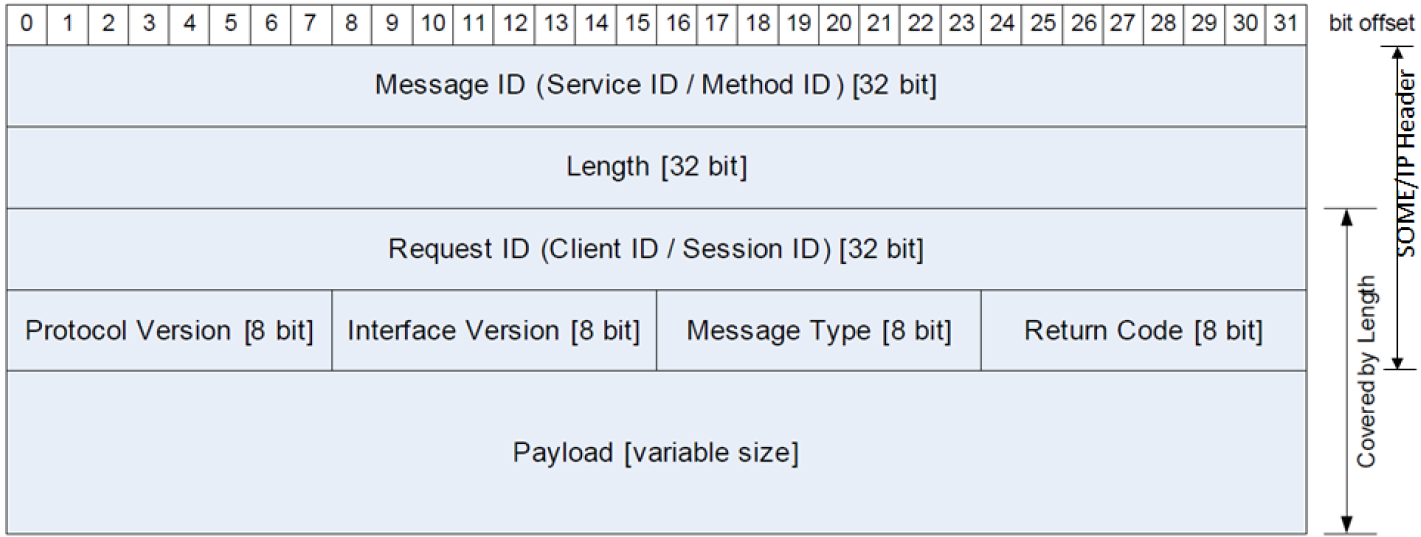
\includegraphics[width=1\textwidth]{Images/chapter2/HeaderSomeip.png}
    \vspace{0.5cm}
    \caption{Structure of \gls{SOMEIP} message format}
    \label{fig:someip_structure}
\end{figure}

The most important header field is the {Message ID}, which is divided into a Service ID and a Method/Event ID. This allows the receiver to identify which service and operation the message belongs to. The {Length} field defines the size of the remaining SOME/IP message, while the {Request ID} combines Client ID and Session ID to match requests with responses. The {Protocol Version} and {Interface Version} fields support compatibility checks between different protocol or service-interface versions. The {Message Type} indicates whether the message is a request, response, notification, or error, and the {Return Code} reports the processing result, such as successful execution or an unknown method.

The payload carries the actual application data, such as method parameters, return values, or event content. SOME/IP defines serialization rules to convert structured data into a linear byte stream suitable for network transmission. These rules cover primitive data types, structures, arrays, strings, unions, and optional extensions. Consistent serialization is essential because ECUs from different suppliers must interpret the same message layout correctly. In addition, SOME/IP supports extensible serialization mechanisms such as tag-length-value (TLV), which allow future members to be added while older receivers can skip unknown fields. This improves long-term compatibility in vehicle software platforms.

\subsubsection{SOME/IP Communication Patterns}

SOME/IP supports several communication patterns that map directly to service-oriented design. The first pattern is {request/response}, where a client sends a request and the provider returns either a response or an error. This pattern is suitable for service operations that require confirmation, such as querying a configuration value or requesting a diagnostic operation. The second pattern is \textbf{fire-and-forget}, where the client sends a request without expecting a response. This is useful for lightweight commands where confirmation is not required.

\begin{figure}[h]
    \centering
    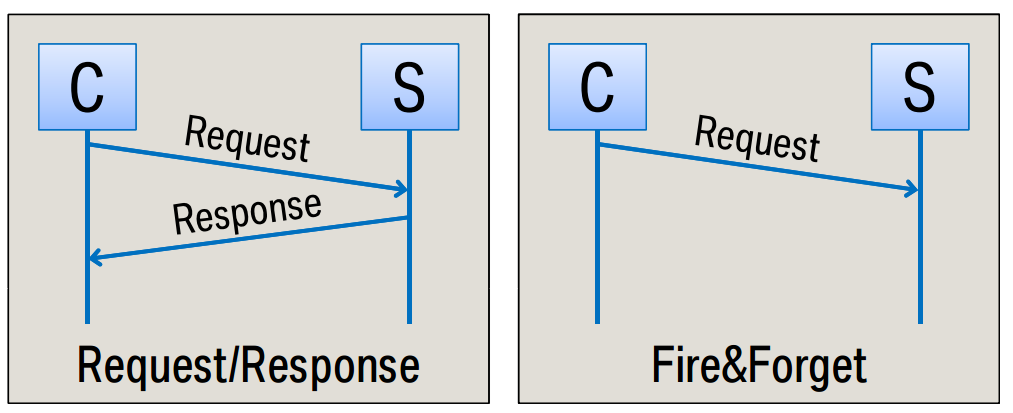
\includegraphics[width=0.8\textwidth]{Images/chapter2/MethodSomeip.png}
    \vspace{0.5cm}
    \caption{Methods in \gls{SOMEIP} \cite{open_alliance_someip}}
\end{figure}

The third pattern is {event notification}. Events follow a publish/subscribe model: a provider publishes notifications, and clients receive them only after subscribing to the relevant event group. Events may be cyclic, such as periodically transmitted vehicle speed, or on-change, such as a door-open state update. Fields extend the event concept by representing persistent service state. A field may provide a getter to read the current value, a setter to modify the value, and a notifier to inform subscribers when the value changes. Thus, events are suitable for streaming or momentary updates, while fields are suitable for state synchronization.

\begin{figure}[h]
    \centering
    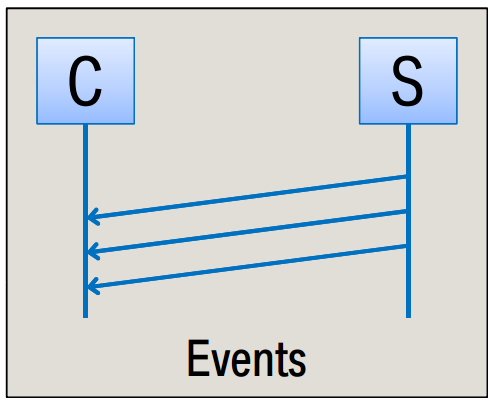
\includegraphics[width=0.45\textwidth]{Images/chapter2/EventSomeip.png}
    \vspace{0.5cm}
    \caption{Events in \gls{SOMEIP} \cite{open_alliance_someip}}
\end{figure}

Error handling is integrated into the protocol through the Return Code field and dedicated ERROR messages. For example, a provider may return an error if a method is unknown, a message is malformed, or an interface version is incompatible. These mechanisms help applications detect communication faults and handle them in a controlled manner.

\subsubsection{SOME/IP Service Discovery}

SOME/IP Service Discovery (SOME/IP-SD) manages the dynamic availability of service instances in an Ethernet network. Instead of hard-coding all communication partners, providers announce available services and clients search for the services they require. This supports the dynamic service-oriented behavior expected in Adaptive AUTOSAR systems.

\begin{figure}[h]
    \centering
    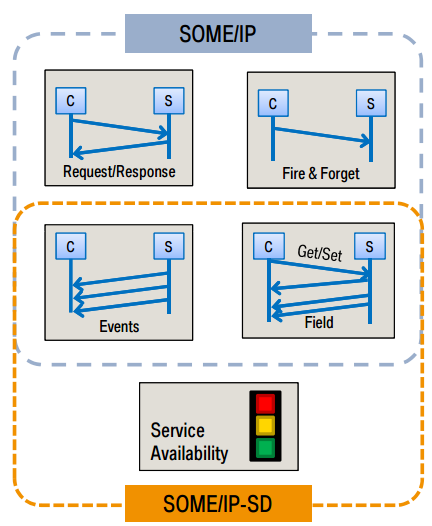
\includegraphics[width=0.5\linewidth]{Images//chapter2/someip_sd.png}
    \vspace{0.5cm}
    \caption{SOME/IP Service Discovery \cite{open_alliance_someip}}
    \label{fig:someip_sd}
\end{figure}

The basic discovery mechanism is based on \texttt{OfferService} and \texttt{FindService}. When a provider becomes available, it sends \texttt{OfferService} messages to announce the service instance. If a client needs a service that has not yet been offered, it sends a \texttt{FindService} message. The Time-To-Live (TTL) value in these messages indicates how long the service information remains valid; a TTL of zero indicates that the service is no longer available.

For event-based communication, SOME/IP-SD also manages subscriptions. After discovering a service, a client sends a \texttt{SubscribeEventgroup} request to receive selected events. The provider replies with \texttt{SubscribeEventgroupAck} or \texttt{SubscribeEventgroupNack}. Only after a successful subscription does the provider send event notifications to the client. Endpoint Options are used to connect abstract service information to concrete network parameters such as IP address, transport protocol, and port number. This separation allows service discovery to remain compact while still providing the information required for runtime communication.

\subsubsection{SOME/IP Transport Layer Bindings}

SOME/IP can be transported using UDP, TCP, or SOME/IP Transport Protocol (SOME/IP-TP). The choice depends on payload size, latency requirements, and reliability expectations. {UDP} is lightweight and connectionless, making it suitable for small, frequent, low-latency messages such as cyclic signals or fire-and-forget communication. It also supports multicast, which is required for many event notification scenarios. However, standard UDP binding is limited by the Ethernet MTU, so payloads are typically restricted to about 1400 bytes, and delivery is not guaranteed.

{TCP} provides reliable, ordered, connection-oriented transmission and can carry larger payloads. It is appropriate for data where correctness is more important than minimum latency, such as diagnostic information or larger configuration data. The trade-off is higher overhead, connection management complexity, and no multicast support.

{SOME/IP-TP} is a protocol extension over UDP that enables segmentation of large SOME/IP messages. It allows large payloads to be split into smaller UDP-compatible segments and reassembled by the receiver. This is useful when large data must be transported with lower latency than TCP. However, it increases receiver complexity because missing, duplicated, or out-of-order segments must be handled carefully.

\begin{table}[h!]
\centering
\renewcommand{\arraystretch}{1.3}
\begin{tabularx}{\textwidth}{|l|X|X|X|}
\hline
\textbf{Feature} & \textbf{UDP Binding} & \textbf{TCP Binding} & \textbf{SOME/IP-TP} \\ \hline
\textbf{Main property} & Lightweight and connectionless. & Reliable and connection-oriented. & Segmentation extension over UDP. \\ \hline
\textbf{Payload size} & Small payloads, typically up to about 1400 bytes. & Large payloads over a stream connection. & Large payloads split into UDP segments. \\ \hline
\textbf{Reliability} & Best-effort; loss is handled by the application. & Reliable, ordered delivery. & Depends on UDP; reassembly fails if required segments are missing. \\ \hline
\textbf{Typical use case} & Small cyclic data, events, multicast notifications. & Diagnostics, configuration data, larger reliable transfers. & Large low-latency data where TCP overhead is undesirable. \\ \hline
\end{tabularx}
\caption{Comparison of SOME/IP Transport Layer Bindings}
\label{tab:someip_transport_comparison}
\end{table}

In summary, SOME/IP provides a service-oriented middleware layer for Ethernet-based automotive systems. Its service model, message format, discovery mechanism, and transport bindings allow Adaptive AUTOSAR applications to communicate in a modular and scalable way. Although the final prototype in this project uses DDS for the implemented data path, SOME/IP remains important background knowledge because it is a major communication technology supported by Adaptive AUTOSAR and is widely used in service-oriented automotive architectures.

\subsection{Data Distribution Service (DDS)}

The ongoing transformation of the automotive industry toward Software-Defined Vehicles (SDVs) and high-performance computing platforms necessitates a fundamental paradigm shift in in-vehicle communication architectures. As Advanced Driver Assistance Systems (ADAS) and autonomous driving frameworks continue to evolve in complexity, the constraints of static, signal-based network topologies---such as the Controller Area Network (CAN) and the Local Interconnect Network (LIN)---become increasingly apparent. The AUTOSAR Adaptive Platform directly addresses these limitations by enforcing a Service-Oriented Architecture (SOA), which utilizes modern middleware solutions to decouple software application components from the underlying hardware and network topology. Within this architectural paradigm, the Data Distribution Service (DDS) operates as a paramount network binding protocol, offering a highly scalable, real-time, and strictly data-centric communication layer. DDS delivers the rigorous temporal determinism required by safety-critical automotive applications, while simultaneously affording the dynamic structural flexibility necessary for complex, distributed machine learning pipelines, sensor fusion networks, and high-bandwidth telemetry systems.

\subsubsection{Service Definition}

Following the specification of Data Distribution Service (DDS) protocol in Adaptive AUTOSAR~\cite{autosar_dds}, DDS is a comprehensive, open international machine-to-machine middleware standard developed, governed, and maintained by the Object Management Group (OMG). Functioning as a data-centric communication protocol, DDS abstracts the complexities of the underlying operating system, the network transport layer, and low-level data serialization formats. This abstraction layer enables seamless, distributed software application communications across highly heterogeneous hardware architectures and diverse programming languages, bridging the gap between embedded microcontrollers and high-performance computing clusters.

At its foundational core, the DDS standard establishes the concept of a virtual ``Global Data Space.'' Within this logical construct, distributed applications can asynchronously share information without requiring direct point-to-point connections. Participating nodes within the network do not exchange opaque, unstructured messages; instead, they read and write strongly typed data-objects. These data-objects are uniquely addressed by an application-defined name, known as a ``Topic,'' combined with a specific cryptographic or logical ``Key'' that identifies discrete, localized instances of that data. The DDS specification rigorously defines both the Application Programming Interfaces (APIs) and the underlying communication semantics required to facilitate this highly structured exchange between data providers and data consumers.

\begin{figure}[h]
    \centering
    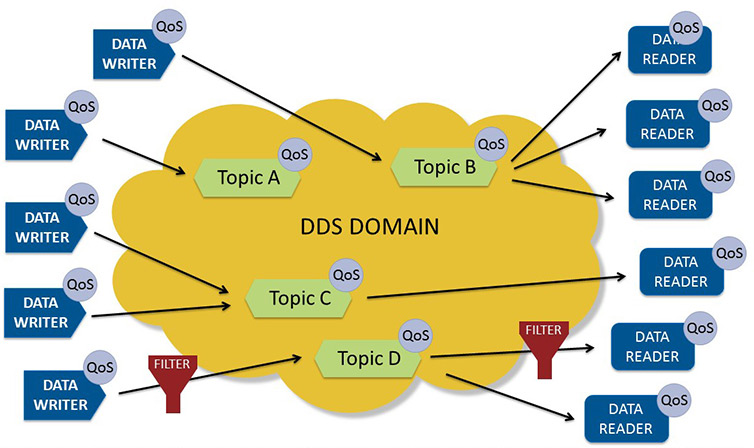
\includegraphics[width=0.8\textwidth]{Images/chap3/dds.jpg}
    \vspace{0.5cm}
    \caption{DDS enables QoS-controlled data-sharing via a publish/subscribe model on named Topics, featuring time/content filtering and strict isolation between independent domains.}
    \label{fig:dds}
\end{figure}

Unlike traditional Remote Procedure Call (RPC) frameworks or conventional Message-Oriented Middleware (MOM), DDS focuses intrinsically and exclusively on the data itself. The middleware is inherently aware of the data schema, strictly defined using the OMG Interface Definition Language (IDL) or the Extensible and Dynamic Topic Types for DDS (DDS-XTypes) specification. This profound data awareness allows the middleware stack to autonomously perform complex content-based filtering, data lifecycle management, and state propagation without requiring application-level intervention. 

The definition of DDS extends beyond mere data transfer; it encapsulates a holistic ecosystem for real-time state management. By standardizing serialization, discovery, security, and delivery guarantees, DDS allows automotive software engineers to concentrate exclusively on application-level logic rather than network-level fault tolerance, fundamentally accelerating the development cycle.



\subsubsection{Public-Subscribe Communication Model}

The architectural foundation of the Data Distribution Service is the Data-Centric Publish-Subscribe (DCPS) model. The DCPS model distinguishes itself by prioritizing the management of stateful data over the mere routing of transient, stateless events. Information is strictly typed and categorized into distinct Topics, and the fundamental unit of information sharing is the structured data-object within these Topics.

The overarching boundary within the DCPS model is the \texttt{Domain}, representing a logically isolated communication space. Applications operating within different domains cannot communicate with one another. An application enters a domain by instantiating a \texttt{DomainParticipant}, which serves as the primary factory and container for all subsequent DDS entities, managing the discovery of other participants within the domain.

Data production is managed by \texttt{Publisher} entities, which act as organizational factories for \texttt{DataWriter} objects. A \texttt{DataWriter} is strongly typed to a specific Topic and is the sole authorized mechanism through which an application can introduce new data samples into the Global Data Space. Conversely, data consumption is handled by \texttt{Subscriber} entities, which function as factories for \texttt{DataReader} objects. A \texttt{DataReader} securely binds to a specific Topic and provides the receiving application with access to the incoming data samples through asynchronous callbacks or synchronous polling.

A defining characteristic of the DCPS model is its robust type system and the critical distinction between ``Instances'' and ``Samples.'' When a Topic data type is defined, specific fields can be explicitly annotated with a \texttt{@key} identifier. The unique mathematical combination of these key values identifies a specific ``Instance'' of the Topic. Every time a \texttt{DataWriter} publishes data for a specific key combination, it generates a new ``Sample'' of that Instance, representing an update to its state. This deeply data-centric approach ensures that subscribers are not merely receiving disconnected packets, but are instead maintaining a synchronized, localized object model that accurately reflects the distributed state of the environment.

\subsubsection{Quality of Service (QoS) Policies}

The defining technical superiority of DDS lies in its extensive Quality of Service (QoS) framework. DDS provides distinct, configurable QoS policies that strictly dictate the behavior of the middleware, decisively separating the functional requirement for data transfer from the implementation of network retries, pacing, and acknowledgments.

Each entity within the DCPS model possesses an associated QoS configuration. A fundamental principle governing DDS QoS is the Request/Offer semantic. A \texttt{DataReader} explicitly requests a certain level of service, and a \texttt{DataWriter} explicitly offers a specific level of service. For a communication channel to be successfully established (matching), the offered QoS must meet or exceed the requested QoS. If incompatible, the middleware prevents association and alerts the application.

The most critical QoS policies utilized within real-time automotive systems include:

\begin{table}[h!]
\centering
\renewcommand{\arraystretch}{1.3}
\begin{tabular}{|p{0.18\textwidth}|p{0.2\textwidth}|p{0.55\textwidth}|}
\hline
\textbf{QoS Policy} & \textbf{Target Entity} & \textbf{Description and Automotive Application} \\
\hline
\textbf{Reliability} & Writer, Reader, Topic & Defines if delivery is guaranteed. \texttt{BEST\_EFFORT} (no retransmissions) suits high-frequency sensor streams. \texttt{RELIABLE} enforces TCP-like reliability over UDP, mandated for safety-critical state transitions. \\
\hline
\textbf{Durability} & Writer, Reader, Topic & Controls data availability to late-joining subscribers. \texttt{VOLATILE} only serves active readers. \texttt{TRANSIENT\_LOCAL} automatically forwards stored past samples to new readers, critical for initialization states. \\
\hline
\textbf{History} & Writer, Reader, Topic & Dictates local cache management. \texttt{KEEP\_LAST} stores only the most recent $N$ samples. \texttt{KEEP\_ALL} retains every sample until successfully delivered to all reliable readers. \\
\hline
\textbf{ResourceLimits} & Writer, Reader, Topic & Governs maximum physical memory allocation (queue bounds). Crucial for embedded ECUs to prevent out-of-memory exceptions during runtime. \\
\hline
\textbf{DestinationOrder} & Writer, Reader, Topic & Determines logical message order during simultaneous writes. Ordering by \texttt{SOURCE\_TIMESTAMP} ensures deterministic behavior in multi-sensor fusion algorithms. \\
\hline
\textbf{Lifespan} & Writer, Reader, Topic & Sets the relevance duration of a sample. Expired data is automatically purged, mathematically guaranteeing that ADAS modules do not react to stale perceptions. \\
\hline
\textbf{UserData} & Participant, Reader, Writer & Attaches custom byte sequences. AUTOSAR specifically utilizes this during discovery to encode Service IDs and contract versions in participant announcements. \\
\hline
\textbf{Liveliness} & Writer, Reader, Topic & Asserts the time interval a node must demonstrate activity. If a sensor node fails to assert liveliness, subscribers are alerted to transition to a safe state. \\
\hline
\end{tabular}
\end{table}

\subsubsection{DDS Real-Time Publish Subscribe (RTPS) Protocol}

While the DDS specification defines the APIs and QoS semantics, the physical interoperability of disparate DDS implementations is governed by the Real-Time Publish Subscribe (RTPS) protocol. Standardized as the DDSI-RTPS, this specification guarantees that a lightweight sensor node can seamlessly communicate with an HPC node running an enterprise DDS implementation, irrespective of the underlying vendor.

RTPS leverages the connectionless, best-effort, and multicast capabilities of UDP/IP to achieve massive scalability, while independently layering a sophisticated reliability protocol on top of it. The RTPS architecture is structurally divided into two primary operational modules: the Discovery Module and the Behavior Module.

The Discovery Module is responsible for the dynamic ``plug-and-play'' nature of DDS. It operates in two sequential phases: the Simple Participant Discovery Protocol (SPDP) and the Simple Endpoint Discovery Protocol (SEDP). During SPDP, \texttt{DomainParticipants} periodically multicast compact announcement messages containing their GUIDs, locators, and basic QoS settings. Upon receiving an unknown announcement, participants initiate the SEDP phase to directly exchange detailed information regarding their internal \texttt{DataWriters} and \texttt{DataReaders}. This completely decentralized architecture fundamentally eliminates single points of failure.

The Behavior Module defines the strictly regulated message exchanges. To fulfill \texttt{RELIABLE} QoS obligations over UDP, RTPS utilizes a Heartbeat and Negative Acknowledgment (NACK) paradigm. A \texttt{DataWriter} periodically multicasts Heartbeats detailing available sequences. If a \texttt{DataReader} identifies missing sequences, it responds with an ACKNACK, prompting the \texttt{DataWriter} to retransmit only the requested samples. Furthermore, DDSI-RTPS specifies the binary layout of messages, allowing microcontrollers with different native byte architectures to parse the data seamlessly.

\subsubsection{DDS in Adaptive AUTOSAR}

The incorporation of DDS into the AUTOSAR Adaptive Platform provides a highly scalable alternative to SOME/IP. Within the AUTOSAR specification, the Communication Management (\texttt{ara::com}) cluster translates language-agnostic \texttt{ServiceInterface} models into concrete DDS entities, Topics, and RTPS wire payloads.

\textbf{Service Discovery Mechanisms}

The DDS Network Binding provides two methodologies for Service Discovery:

\begin{enumerate}
\item \textbf{Service Discovery via Domain Participant USER\_DATA QoS policy:} This approach natively leverages the built-in RTPS Participant Discovery phase (SPDP). The middleware injects a precisely formatted string into the \texttt{USER\_DATA} QoS policy of its \texttt{DomainParticipant} containing the Service ID, Instance ID, and version. Client proxies parse this string to verify compatibility. Because this utilizes intrinsic DDS discovery traffic without creating additional entities, it is exceptionally resource-efficient.
\item \textbf{Service Discovery via Topic:} For highly complex topologies, the offering service explicitly publishes a dedicated \texttt{ServiceAnnouncementMessage} over a standardized \texttt{ara.com://services/discovery} topic, utilizing the Service ID and Instance ID as cryptographic keys.
\end{enumerate}

\textbf{Mapping of Events and Triggers}

An \texttt{Event} maps fundamentally to a single, dedicated DDS Topic. The payload is serialized into an IDL struct that inevitably includes an \texttt{@key uint16 instance\_id} field alongside the data. This key ensures logical segregation by the middleware's management queues. \texttt{Triggers} map similarly but are entirely devoid of a functional data payload; they utilize merely the key to serve as an asynchronous signaling mechanism.

\textbf{Mapping of Fields}

A \texttt{Field} is systematically decomposed for network transmission. If it possesses a notification property, a dedicated DDS Topic pushes state updates like an Event. If it has getter or setter attributes, a Request/Reply Topic pair is generated identically to the Method mapping, enabling RPC over DDS state management.

\textbf{Data Serialization and Security Integration}

The DDS binding relies on the OMG DDS-XTypes specification for data serialization, seamlessly handling complex C++ structures while managing byte-endianness transparently. 

For security, the binding natively supports the OMG DDS-Security standard via a plugin architecture, providing Authentication, Access Control, and Cryptography at the individual submessage level. AUTOSAR mandates that Adaptive Applications must enforce Identity and Access Management (IAM) grants through deployed DDS Security policies, allowing for highly granular configurations that minimize cryptographic overhead while maximizing real-time throughput.




\subsection{AUTOSAR Runtime for Adaptive applications (\texttt{ara})}

\begin{figure}[h]
    \centering
    \includegraphics[width=0.9\textwidth]{Images/chapter2/AP_Arch.png}
    \vspace{0.5cm}
    \caption{Logical View of AUTOSAR Adaptive Platform Architecture \cite{autosar_sw_arch}}
    \label{fig:autosar_adaptive_arch_logic}
\end{figure}


The AUTOSAR Runtime for Adaptive applications (\texttt{ara}) acts as the standardized runtime environment for Adaptive Applications (AA). It abstracts the underlying system features and provides a uniform interface for applications to interact with the platform. As illustrated in Figure \ref{fig:autosar_adaptive_arch_logic}, the architecture is composed of the following key blocks:

\paragraph*{Adaptive Applications (AA):} These are user applications running on top of the Adaptive Platform. They implement specific automotive functions (e.g., automated driving logic, infotainment) and interact with the platform exclusively through the \texttt{ara} interfaces. This design decouples the application logic from the underlying OS and hardware, ensuring portability.

\paragraph*{ARA Interface:} \texttt{ara} consists of a set of Application Programming Interfaces (APIs), primarily standardized in C++. These interfaces allow AAs to access functionalities provided by the Functional Clusters. From the application's perspective, the interface is uniform regardless of whether the underlying functionality belongs to the Foundation or Services layer.


\paragraph*{Functional Clusters (FC):} Functional Clusters are logical groupings of platform functionality. They are responsible for providing specific services to the applications. They are categorized into two types:

\textbf{Adaptive Platform Foundation:} This layer provides the fundamental functionalities required to run the system and applications. It includes core services such as Execution Management (\texttt{ara::exec}), Communication Management (\texttt{ara::com}), Logging (\texttt{ara::log}), Persistency (\texttt{ara::per}), etc. These clusters behave similarly to operating system services.
    
\textbf{Adaptive Platform Services:} This layer provides platform-standard services that are more domain-specific but still standardized, such as Update and Configuration Management (\texttt{ara::ucm}), State Management (\texttt{ara::sm}), and Network Management (\texttt{ara::nm}).

Under the hood, the implementation of these interfaces may involve library calls within the application's process space or Inter-Process Communication (IPC) with daemon processes, but this complexity is hidden from the application developer.



In the context of this project, our primary focus lies within the Application Layer (Adaptive Applications). Consequently, our discussion will center on the essential Functional Clusters that support application runtime and interaction: Execution Management (\texttt{ara::exec}), Communication Management (\texttt{ara::com}), and Log and Trace (\texttt{ara::log}). Additionally, to address the specific requirements of our machine learning use case, we will integrate non-platform services, specifically utilizing the OpenCV library (namespace \texttt{cv}) for advanced image pre-processing and computer vision tasks. 



\subsection{Execution Management (\texttt{ara::exec})} 

Execution Management is responsible for all aspects of the system execution, including the initialization of the Adaptive Platform and the lifecycle management of Processes. Acting as the entry point of the AUTOSAR Adaptive Platform, Execution Management is started by the Operating System during system boot and subsequently launches the Functional Clusters and Adaptive Applications based on the configuration defined in the Machine Manifest and Execution Manifests.

It controls the startup and shutdown of these Processes according to defined Function Group States, ensuring that the specific set of processes required for a given state are active. While the Operating System performs the actual runtime scheduling, Execution Management configures the OS to enforce scheduling parameters and resource limits. This includes assigning processes to Resource Groups to limit CPU time and memory usage, thereby supporting freedom from interference between applications. Furthermore, Execution Management enables deterministic execution through the \texttt{DeterministicClient} API, allowing for the control of process-internal cycles and data determinism.

To establish a Trusted Platform, Execution Management maintains a chain of trust originating from a Trust Anchor. During authenticated startup, it validates the authenticity and integrity of Adaptive Applications and prevents the execution of any process if security violations are detected.

\subsubsection{Block View Diagram } 

\textbf{Interface for state reporting: }
All processes started by Execution Management (i.e. all processes of the AUTOSAR Adaptive Platform and all processes of Adaptive Applications) shall report their execution state back to Execution Management via the ExecutionClient interface

\begin{figure}[h]
    \centering
    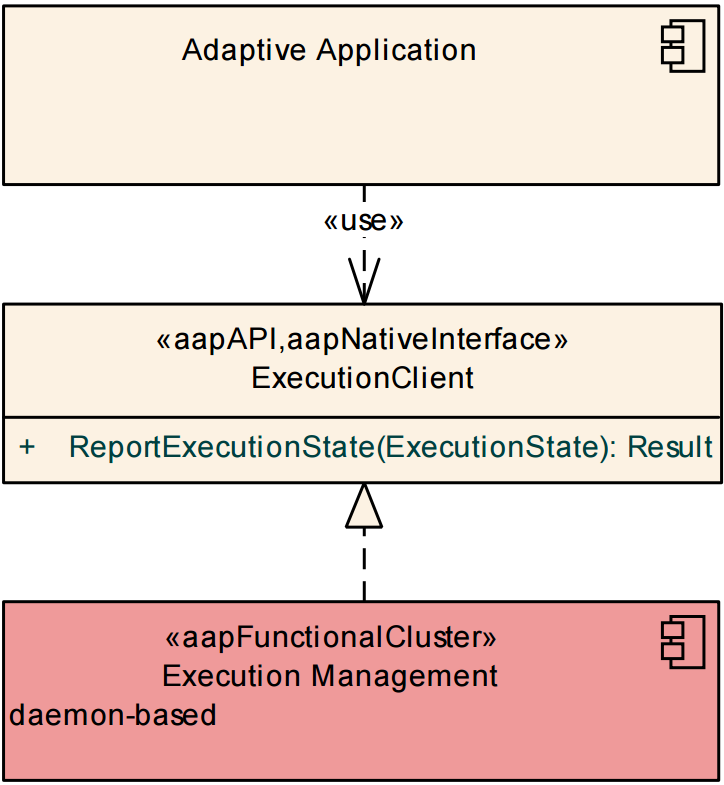
\includegraphics[width=0.5\textwidth]{Images/chapter2/em_interface.png}
    \vspace{0.5cm}
    \caption{Interface for state reporting \cite{autosar_sw_arch}}
    \label{fig:em_interface}
\end{figure}

\textbf{Provided Interfaces:} \texttt{ara::exec::ExecutionClient} will provide the interface reporting the execution state of the process to Execution Management. \texttt{ara::exec::StateClient} will Requests Function Group State transitions and retrieves execution errors.

\begin{figure}[h]
    \centering
    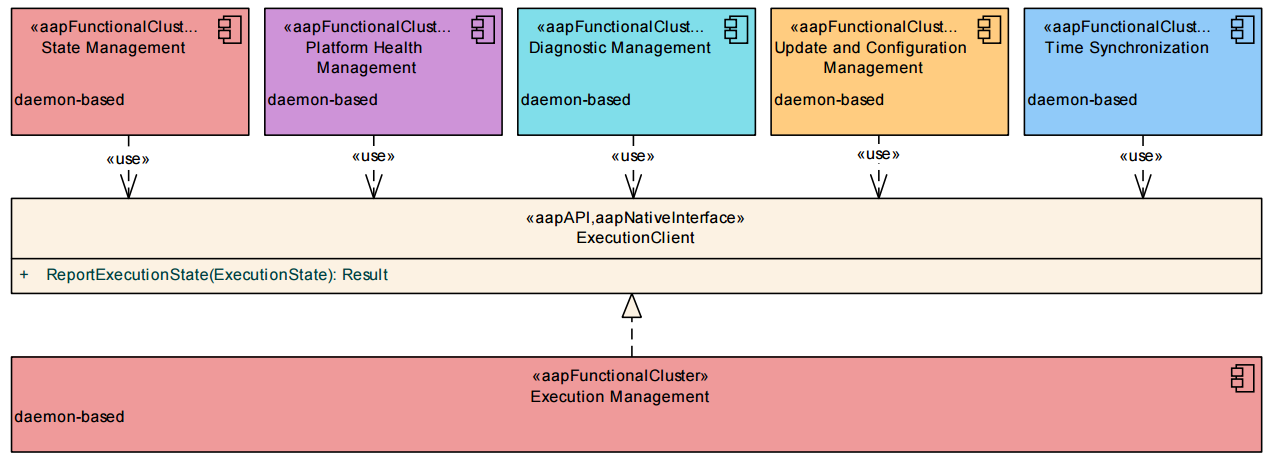
\includegraphics[width=0.9\textwidth]{Images/chapter2/em_provided_execcli.png}
    \vspace{0.5cm}
    \caption{Users of ExecutionClient Interface \cite{autosar_sw_arch}}
    \label{fig:em_provided_execcli}
\end{figure}

\begin{figure}[h]
    \centering
    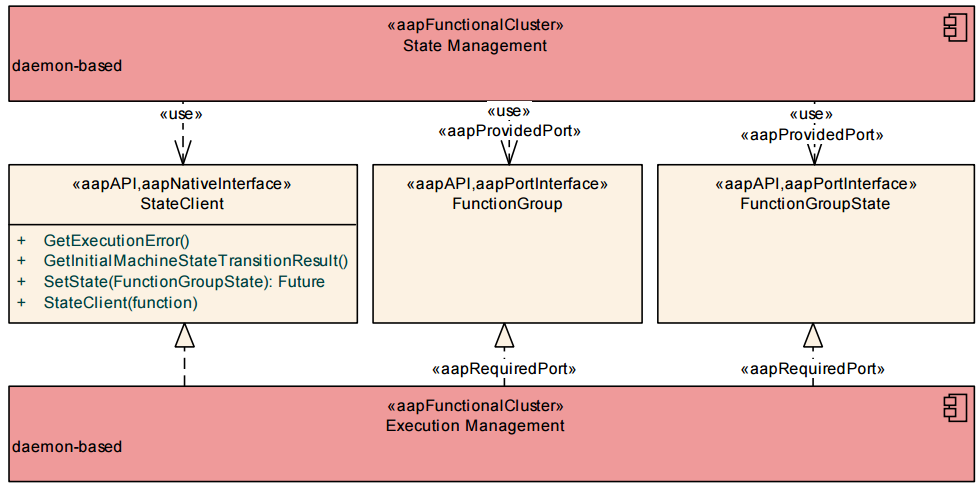
\includegraphics[width=0.9\textwidth]{Images/chapter2/em_provided_sm.png}
    \vspace{0.5cm}
    \caption{Users of State Management Interface \cite{autosar_sw_arch}}
    \label{fig:em_provided_sm}
\end{figure}

\newpage
\textbf{Required Interfaces:} \begin{itemize} 
    \item \texttt{Log and Trace::Logger}: Execution Management shall use this interface to log standardized messages. 
    \item \texttt{Persistency::KeyValueStorage}: Execution Management should use this interface to read and write persistent data. 
    \item \texttt{Platform Health Management::SupervisedEntity}: Execution Management shall use this interface to enable supervision of its process(es) by Platform Health Management. 
    \item \texttt{Time Synchronization::SynchronizedTimeBaseConsumer}: The \texttt{DeterministicClient} implementation in Execution Management should use this interface to synchronize execution. 
    \item \texttt{Manifest Accessor}: Execution Management shall use this interface to read the configuration of its \texttt{DeterministicClient} and information about Function Groups and Processes from the Manifests. 
    \item \texttt{Operating System::Multi-Process System Interface}: Execution Management shall use this interface to start, configure, and control OS-level processes. 
\end{itemize}

\begin{figure}[h]
    \centering
    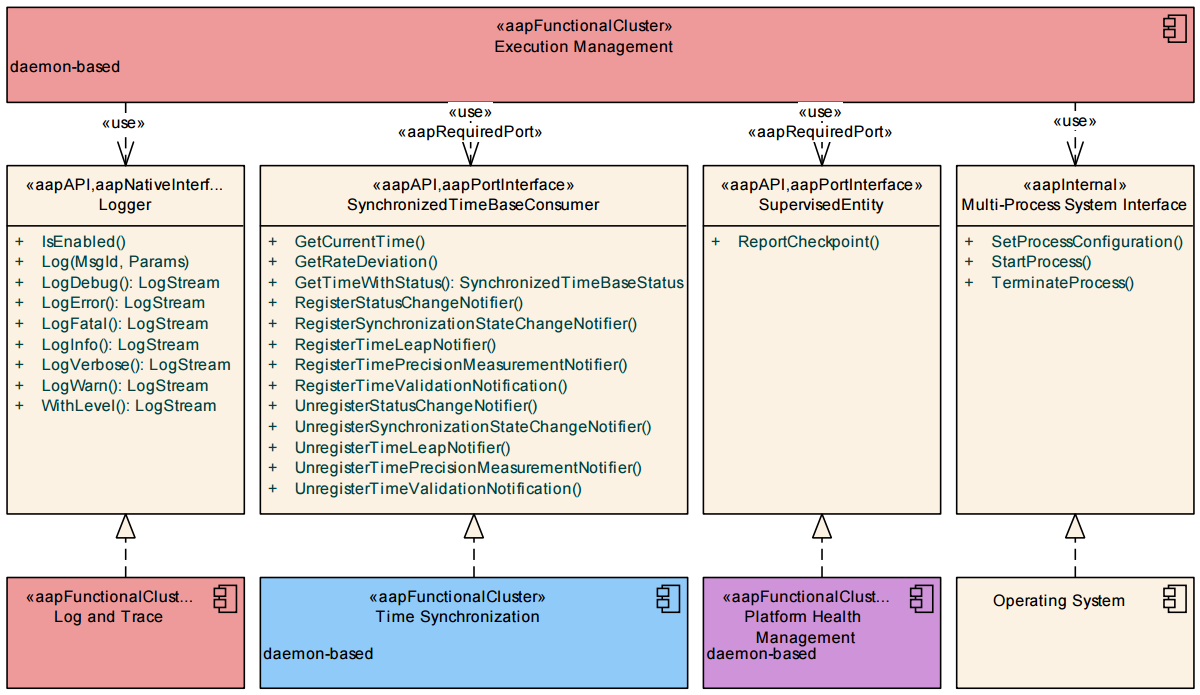
\includegraphics[width=0.9\textwidth]{Images/chapter2/em_required.png}
    \vspace{0.5cm}
    \caption{Required Interfaces of Execution Management \cite{autosar_sw_arch}}
    \label{fig:em_required}
\end{figure}


\newpage
\subsubsection{System Startup} 

\begin{figure}[h]
    \centering
    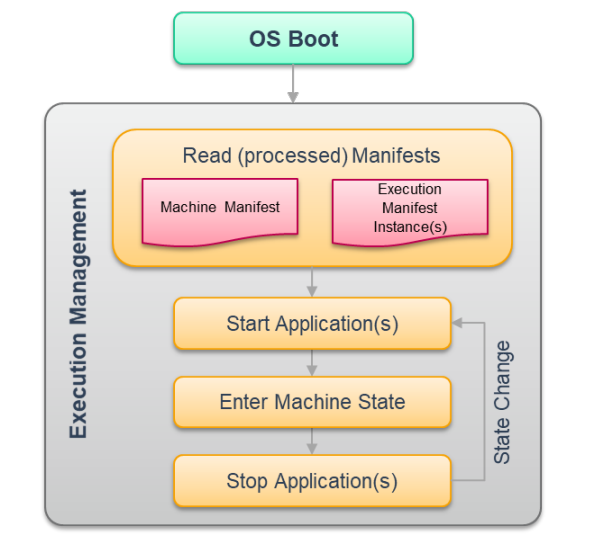
\includegraphics[width=0.5\textwidth]{Images/chapter2/EM_APStartup.png}
    \vspace{0.5cm}
    \caption{AP Startup Sequence \cite{autosar_exec_mgmt}}
    \label{fig:em_ap_startup}
\end{figure}

\textbf{Startup Sequence:} When the Machine is powered on, the Operating System (OS) is initialized first. Immediately following OS initialization, Execution Management is launched as the Platform's initial process. It is then the responsibility of Execution Management to launch the other platform-level processes that constitute the Functional Clusters of the Adaptive Platform Foundation. Once the Adaptive Platform Foundation is fully operational, Execution Management proceeds to launch the processes associated with Adaptive Applications. The specific startup order for both platform-level and application-level processes is determined by Execution Management, utilizing the configuration defined in the Machine Manifest and the dependencies specified in the Execution Manifest.

\textbf{Application Structure:} An Adaptive Application is composed of multiple Executable elements, which generally correspond to executable files located on the filesystem. To allow for flexible behavior, each Executable can define multiple Process configurations (and therefore distinct startup configurations). The active configuration is determined by the specific Function Group States in which the Executable is currently active.

\textbf{Trusted Platform:} To ensure system security, Execution Management optionally supports an authenticated startup process. This mechanism establishes a Trusted Platform by maintaining a chain of trust originating from a Trust Anchor. During this phase, Execution Management validates the authenticity and integrity of applications before they are launched. If any violations are detected during validation, Execution Management will prevent the execution of the compromised application.

\textbf{Manifests:}

\begin{figure}[h]
    \centering
    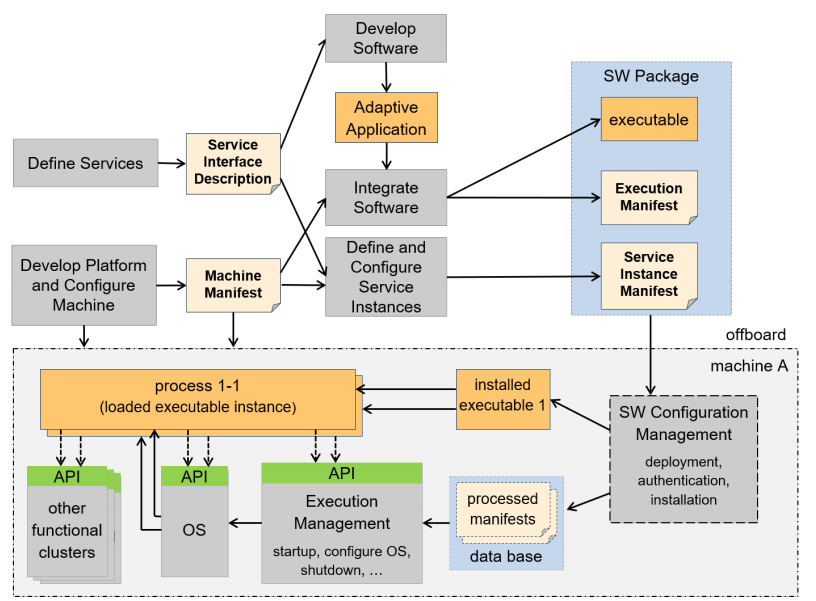
\includegraphics[width=0.9\textwidth]{Images/chapter2/ap_dev_flow.png}
    \vspace{0.5cm}
    \caption{Application Development Flow \cite{autosar_exec_mgmt}}
    \label{fig:ap_dev_flow}
\end{figure}

Manifests serve as the standardized format for description and configuration within the AUTOSAR Adaptive Platform, effectively bridging the gap between system design and runtime execution. To address the distinct phases of the development lifecycle, Manifests are categorized into four specific types. {Application Design} specifies the architectural aspects of the software; while not deployed itself, it aids in defining deployment configurations. The {Execution Manifest} details deployment parameters—such as startup dependencies and resource usage—and is bundled directly with the application executable. Similarly, the {Service Instance Manifest} accompanies the executable code to configure service-oriented communication bindings and transport protocols. Finally, the {Machine Manifest} describes the configuration of the underlying computing machine and the Adaptive Platform foundation, independent of the specific applications hosted on the system. As in Figure \ref{fig:ap_dev_flow}, the application development flow will show how manifests are created. 

\subsubsection{\texttt{ara::exec} Responsibility}

% Execution Management functions as a critical functional cluster within the Adaptive Platform Foundation, serving as the primary entity responsible for managing all aspects of system execution, which encompasses the initialization of the platform as well as the startup and shutdown of Applications. It operates in close conjunction with the Operating System, specifically configuring it to handle the run-time scheduling of Applications. The core unit managed by this cluster is the Modelled Process, which is an instance of an Executable. Execution Management is responsible for the lifecycle of these processes, performing tasks such as creation and termination based on specific information contained within Manifest files, specifically the Execution Manifest and the Machine Manifest.

% A central responsibility of Execution Management is to determine the precise timing and sequence for starting or stopping processes based on the configuration data extracted from the manifests. It derives the launching order of Applications to ensure the proper startup of the AUTOSAR Adaptive Platform, ensuring that processes are started in a sequence that respects declared Execution Dependencies. This dependency management ensures that applications are active only when the services they require are available and are terminated only after their services are no longer required. To maintain strict control over the system, Execution Management is designed to be the sole entity responsible for starting processes and must restrict the rights of the processes it launches so they cannot start other processes themselves.

% In addition to lifecycle management, Execution Management is integral to the platform's State Management. It supports the execution of specific Modelled Processes depending on the current Function Group State or Machine State. Execution Management initiates state transitions, such as the transition from the Off state to the Startup state during the platform's boot phase. During these transitions, it is responsible for terminating processes that are no longer needed in the requested state and starting those that are required, all while monitoring process termination and startup timeouts to ensure the transition completes successfully or handles errors appropriately. While Execution Management facilitates these changes, it hands over the responsibility for requesting subsequent state changes to the State Management cluster after the initial startup transition is confirmed.

% The responsibility of Execution Management extends to the configuration of the Operating System to enable appropriate resource management and scheduling. Although the Operating System performs the actual run-time scheduling, Execution Management is responsible for initializing the OS with the necessary configuration parameters derived from the manifests. This includes the configuration of scheduling policies and priorities for the initial threads of processes, as well as the assignment of processes to specific processor cores. Furthermore, Execution Management supports resource limitation by configuring budgets for CPU usage and memory consumption for groups of processes, ensuring that applications operate within defined constraints to maintain system stability.

% Finally, Execution Management plays a pivotal role in ensuring the security and determinism of the platform. It is responsible for supporting a Trusted Platform by ensuring that the integrity and authenticity of all Executables and their associated data, such as manifests, are verified before any process is started. In the event of a failed check, it executes defined measures to prevent compromised software from running. Additionally, Execution Management provides support for Deterministic Execution, allowing for calculations that are time and data deterministic. This involves providing APIs and mechanisms that support the control of process-internal cycles and deterministic worker pools, which are essential for safety-critical systems requiring reproducible behavior.

Execution Management (\texttt{ara::exec}) is a core functional cluster in the Adaptive AUTOSAR platform. It acts as the main unit for managing system execution, including platform initialization and the lifecycle of applications. Working closely with the Operating System (OS), it creates and terminates processes based on the rules defined in the Execution and Machine Manifest files. A key responsibility is controlling the exact launching order of applications to respect their dependencies. To keep strict control over the system, Execution Management is the only component allowed to start processes, ensuring that applications are active only when their required services are ready.

In addition to lifecycle control, Execution Management plays an important role in State Management and OS configuration. It starts or stops specific processes depending on the current machine or function group state. For example, during the boot phase, it handles the transition from the ``Off'' state to ``Startup,'' ensuring that old processes are terminated and new ones are launched properly. Furthermore, Execution Management configures the OS to manage resources efficiently. Although the OS handles the actual run-time scheduling, Execution Management sets up the initial scheduling policies, assigns processes to specific processor cores, and limits CPU and memory usage to keep the system stable.

Finally, Execution Management ensures the security and reliability of the platform. It supports a Trusted Platform by verifying the integrity and authenticity of all executables and manifests before any process begins. If a check fails, it takes action to stop compromised software from running. Additionally, it supports Deterministic Execution, which is crucial for safety-critical systems. By providing specific mechanisms and APIs, Execution Management guarantees that calculations remain consistent in terms of both time and data, ensuring reproducible and safe behavior across the system.


% \subsubsection{Process Lifecycle Management}

% In the AUTOSAR Adaptive Platform, the lifecycle of a process is viewed from two distinct perspectives: the {Process State}, which is the external view maintained by Execution Management for orchestration, and the {Execution State}, which represents the internal lifecycle from the perspective of the application process itself.

% \begin{figure}[h]
%     \centering
%     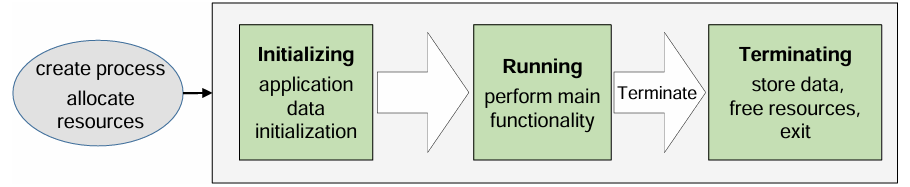
\includegraphics[width=0.8\textwidth]{Images/chapter2/em_execstate.png}
%     \vspace{0.5cm}
%     \caption{EM Execution State \cite{autosar_exec_mgmt}}
%     \label{fig:em_execstate}
% \end{figure}

% Because the process and Execution Management run as independent operating system processes, they execute asynchronously. The Execution State serves as the synchronization mechanism between the application's internal progress and the Execution Management's control logic. This separation allows the internal state of a process to evolve without strictly coupling it to the internal state machine of Execution Management.

% \paragraph*{The Execution State Lifecycle}
% While the API explicitly defines the \texttt{kRunning} state, the full lifecycle includes implied states that dictate how a process initializes, runs, and shuts down.

% \textbf{Initializing (Implied State):}
% The "Initializing" state is an implied state that is not explicitly defined in the \texttt{ExecutionState} enumeration but is recognized operationally by Execution Management. This phase, {Start}, begins immediately when the OS process is created and code execution commences. During the {Activity} phase, the process performs necessary setup tasks, such as memory allocation, variable initialization, and checking configuration files. The state concludes, marked as {End}, when the process explicitly notifies Execution Management that it is ready to operate.

% \textbf{Running (\texttt{kRunning}):}
% The \texttt{kRunning} state is the primary active state defined in the API (\texttt{ara::exec::ExecutionState::kRunning}). A process must explicitly report this state, a {Transition}, to Execution Management once initialization is complete. Regarding {Timing Requirement}, processes are expected to report \texttt{kRunning} after internal initialization but generally before completing Service Discovery. If a process waits until Service Discovery is finished to report \texttt{kRunning}, it may cause non-deterministic delays for other processes that have execution dependencies on it. Once \texttt{kRunning} is reached, the process is considered in its {Operational Context}, ready to perform its main functionality.

% \textbf{Terminating (Implied State):}
% Like initialization, "Terminating" is a state characterized by the reaction to a termination request rather than a specific API call from the process. The {Trigger} for this phase is Execution Management sending a \texttt{SIGTERM} signal to the process. Upon receiving \texttt{SIGTERM}, the {Activity} involves the process saving persistent data, closing file handles, and freeing resources. The {Completion} of this state occurs when the process exits with the status \texttt{EXIT\_SUCCESS} (0).

% \paragraph*{API and Reporting Mechanism}
% To synchronize with Execution Management, processes utilize the \texttt{ara::exec::ExecutionClient} class. The {Reporting API} allows the process to report its state using the method \texttt{ReportExecutionState}, for example, \texttt{ReportExecutionState(kRunning)}. The {Scope of Authority} restricts a process to reporting only its own Execution State. Execution Management performs {Validation} on state transitions; if a process attempts to report \texttt{kRunning} when Execution Management believes the process is already in a state other than "Starting" (e.g., if it is already running), the API will return the error \texttt{kInvalidTransition}.

% \paragraph*{Process Categorization: Reporting vs. Non-Reporting}
% Execution Management supports two distinct behaviors regarding Execution State reporting, configured via the Execution Manifest.

% \textbf{Reporting Processes:}
% This is the standard behavior for AUTOSAR Adaptive Applications. These processes exhibit a specific \textbf{Behavior} where they are aware of the \texttt{ara::exec} API and explicitly call \texttt{ReportExecutionState(kRunning)}. For {Synchronization}, Execution Management waits for this specific report before considering the process to be in the "Running" Process State.

% \textbf{Non-Reporting Processes:}
% This category supports legacy applications or prototypes that were not designed with the AUTOSAR Adaptive Platform in mind and do not contain AUTOSAR-specific API calls. Their {Behavior} is characterized by not calling \texttt{ReportExecutionState}. Instead, an {Implicit Transition} occurs where Execution Management treats these processes as "Running" immediately after the OS process is created and resources are allocated. {Restrictions} apply: if a configured Non-reporting Process attempts to use the API to report its state, Execution Management considers this a violation and returns a \texttt{kCommunicationError}. Due to {Limitations}, because they effectively skip the "Initializing" phase from EM's perspective, "Running" execution dependencies are satisfied immediately upon process creation, which may require the use of a "Companion Process" to bridge dependency gaps.

% \paragraph*{Termination and Error Handling:}
% Proper lifecycle management requires strict adherence to termination protocols. {Graceful Termination} requires a process to exit with status 0 (\texttt{EXIT\_SUCCESS}) to indicate a successful shutdown. In contrast, an {Unexpected Termination} occurs if a process exits with a non-zero status, or if it terminates before reporting \texttt{kRunning}, which Execution Management classifies as such. The {Consequences} of an unexpected termination trigger error handling within the State Management functional cluster, setting the affected Function Group to an "Undefined Function Group State" and reporting an \texttt{ExecutionError}.



% The {Process State} is the internal state machine maintained by Execution Management to track the lifecycle of a Modelled Process. While the Execution State reflects the application's internal progress, the Process State reflects Execution Management's orchestration view. Execution Management maintains this state independently to manage timeouts, handle errors, and resolve Execution Dependencies without being strictly coupled to the internal logic of the application process.

% \begin{figure}[h]
%     \centering
%     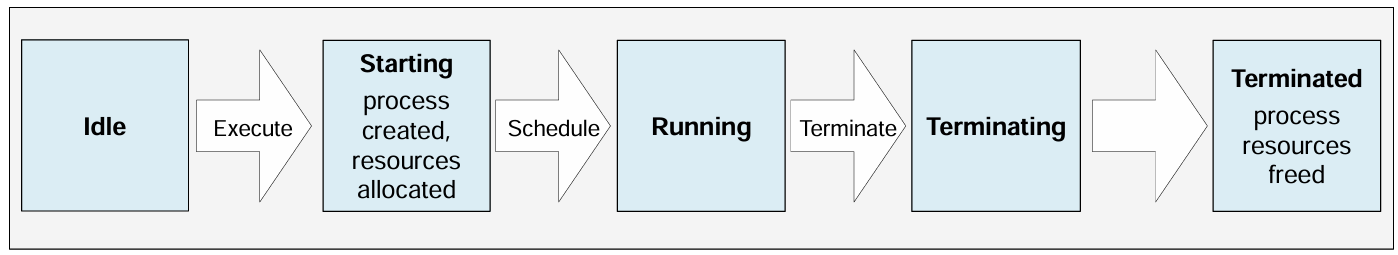
\includegraphics[width=0.9\textwidth]{Images/chapter2/em_processstate.png}
%     \vspace{0.5cm}
%     \caption{Process State \cite{autosar_exec_mgmt}}
%     \label{fig:em_processstate}
% \end{figure}

% \paragraph*{The Process State Lifecycle}
% The lifecycle of a process, as managed by Execution Management, consists of five distinct states. Transitions between these states are driven by API calls, OS signals, and internal configuration logic.

% \textbf{Idle:} The Idle state represents the dormancy of a process. This state applies prior to the creation of the Operating System (OS) process and prior to the allocation of any OS resources. In this state, the process exists only as a configuration entry in the Execution Manifest. It consumes no CPU time or memory. The process leaves the Idle state when Execution Management initiates the startup sequence required by a Function Group State change.

% \textbf{Starting:} The Starting state covers the physical launch and initialization phase of the process. Execution Management transitions a process to ``Starting" immediately upon creating the OS process and allocating the necessary resources. During this phase, Execution Management monitors the ``Startup Timeout." This is the time allowed between the request for process creation and the process successfully reporting \texttt{kRunning}. To ensure state consistency, if a Reporting Process attempts to report \texttt{kRunning} but Execution Management does not consider it to be in the "Starting" state (e.g., if it is already Running), the API call is rejected with the error \texttt{kInvalidTransition}.

% \textbf{Running:} The Running state indicates that the process is fully active and functional. The criteria for entering this state vary by process configuration:
% The process transitions to "Running" only after it explicitly reports the \texttt{kRunning} Execution State via the API. This serves as a synchronization barrier, ensuring dependent processes do not start until this process is truly ready. Because these processes do not use the AUTOSAR API, Execution Management implicitly transitions them to "Running" immediately after resource allocation and process creation. If a process fails to reach the "Running" state within the configured timeout, Execution Management may attempt to restart it a configured number of times (\texttt{numberOfRestartAttempts}) before declaring a failure and stopping the Function Group State transition.

% \textbf{Terminating:} The Terminating state represents the shutdown phase where the process is expected to release resources and save data. This state applies from the moment Execution Management sends the \texttt{SIGTERM} signal to the process. Execution Management monitors the time the process spends in this state. If the process does not exit within the configured termination timeout, Execution Management considers the process unresponsive and requests the Operating System to forcibly terminate it (typically via \texttt{SIGKILL}). Even if a timeout occurs and forced termination is required, Execution Management continues the state transition to ensure the target Function Group State is eventually reached.

% \textbf{Terminated:} The Terminated state marks the successful conclusion of a process execution instance. This state applies after the process has successfully exited and all process resources have been freed by the Operating System. Execution Management detects this state by observing the exit status of the OS process (e.g., utilizing \texttt{waitpid} on POSIX systems). A normal termination requires an exit status of \texttt{EXIT\_SUCCESS} (0). Any other exit code, or termination by an unhandled signal, is classified as an "Unexpected Termination".


% Although both Idle and Terminated implies that no code is executing and no resources are allocated, Execution Management treats them as semantically distinct for dependency resolution. In {Idle} state, the process has not run in the current lifecycle context. In {Terminated} state, the process has run, finished its task, and shut down gracefully. This distinction allows for Self-Terminating Processes. A dependent process can be configured to start only after a provider process has reached the "Terminated" state (e.g., "Start Data Analyzer" only after "Data Collector" is "Terminated"). This dependency cannot be satisfied if the provider is merely "Idle".

% \paragraph*{Error Handling and Unexpected States:}
% Execution Management actively monitors processes for deviations from the expected lifecycle. {Unexpected Termination:} If a process terminates without a request (or exits with a non-zero status) while in the Running state or during startup, Execution Management flags this as an Unexpected Termination. {Consequences:} The event is logged. The Function Group to which the process belongs is set to an Undefined Function Group State. An \texttt{ExecutionError} is reported via the State Client API to allow State Management to decide on recovery actions (e.g., restarting the Machine or switching to a safe state).

% \paragraph*{Role in Execution Dependencies:}
% Process States are the fundamental building blocks for defining startup and shutdown sequencing in the Execution Manifest. Dependencies are defined as \texttt{<Process>.<State>} pairs. 
% \begin{itemize}
%     \item \textbf{Running Dependency:} Ensures a service provider is fully operational before a dependent consumer starts. The dependent waits for the provider to reach the Running Process State. 
%     \item \textbf{Terminated Dependency:} Used primarily for sequential tasks. The dependent waits for the provider to reach the Terminated Process State. 
%     \item \textbf{Scope Constraint:} Execution Management only resolves dependencies within a single Function Group State. It considers it an error if a process depends on another process that is not part of the same Function Group State.
% \end{itemize}

\subsubsection{Process Lifecycle Management}

In the AUTOSAR Adaptive Platform, process lifecycle management operates on two distinct but synchronized levels: the {Execution State} (the application's internal perspective) and the {Process State} (the orchestration perspective maintained by Execution Management). Because the application and Execution Management run asynchronously as independent OS processes, these dual states decouple internal initialization logic from the broader system state machine.

\paragraph*{The Execution State (Application Perspective)}
The Execution State in the Figure~\ref{fig:em_execstate} represents the application's internal lifecycle. Upon OS process creation, an application implicitly enters an "Initializing" phase to allocate resources and perform setup tasks. Once initialization is complete (but crucially, before finalizing Service Discovery to avoid dependency deadlocks), a standard AUTOSAR process must explicitly notify Execution Management by calling \texttt{ara::exec::ExecutionClient::ReportExecutionState(kRunning)}. When the application needs to shut down---typically triggered by a \texttt{SIGTERM} signal from Execution Management---it implicitly enters the "Terminating" phase, releases resources, and concludes by exiting with \texttt{EXIT\_SUCCESS} (0) to signal a graceful termination.

\begin{figure}[h]
    \centering
    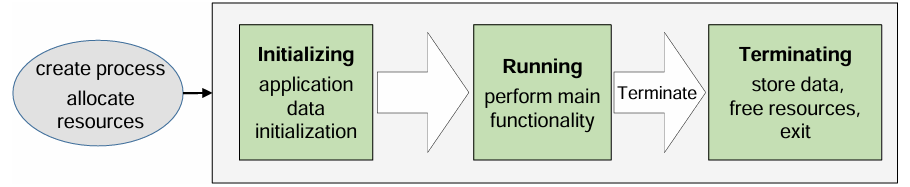
\includegraphics[width=0.8\textwidth]{Images/chapter2/em_execstate.png}
    \vspace{0.5cm}
    \caption{EM Execution State \cite{autosar_exec_mgmt}}
    \label{fig:em_execstate}
\end{figure}

\paragraph*{The Process State (Orchestration Perspective)}
Conversely, the Process State is maintained internally by Execution Management to resolve execution dependencies, manage timeouts, and enforce error handling. The lifecycle encompasses five states, which is presented in Figure~\ref{fig:em_processstate}:
\begin{itemize}
    \item \textbf{Idle:} The process exists only as a configuration entry; no OS resources are allocated.
    \item \textbf{Starting:} The OS process is created, and Execution Management monitors a "Startup Timeout" while waiting for the application to report readiness.
    \item \textbf{Running:} The process has successfully reported \texttt{kRunning}. Dependent applications configured with a "Running Dependency" on this process are now permitted to start. (Note: Non-AUTOSAR legacy applications are implicitly transitioned to this state immediately after OS creation).
    \item \textbf{Terminating:} Execution Management has issued a \texttt{SIGTERM} and monitors a termination timeout. If the process hangs, it is forcibly terminated via \texttt{SIGKILL}.
    \item \textbf{Terminated:} The OS process has successfully exited. This distinct state enables "Terminated Dependencies" for sequential task execution.
\end{itemize}

\begin{figure}[h]
    \centering
    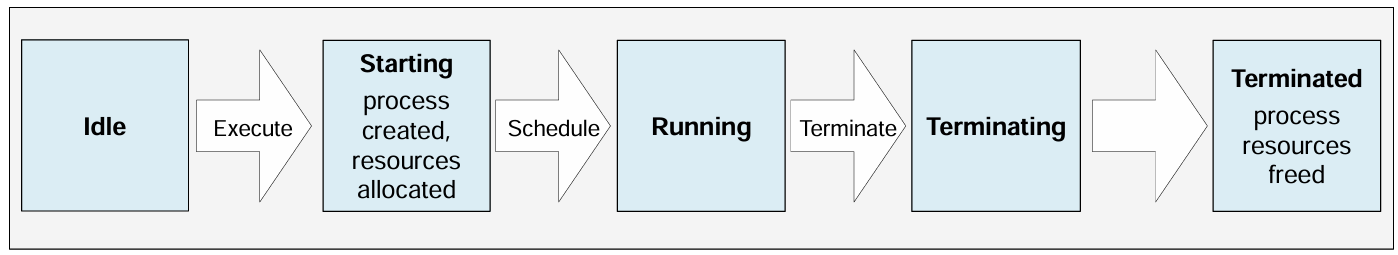
\includegraphics[width=0.9\textwidth]{Images/chapter2/em_processstate.png}
    \vspace{0.5cm}
    \caption{Process State \cite{autosar_exec_mgmt}}
    \label{fig:em_processstate}
\end{figure}

Strict error handling is enforced throughout this lifecycle. If a process exits with a non-zero status or terminates unexpectedly while running, Execution Management logs the event, flags the associated Function Group with an "Undefined Function Group State," and reports an \texttt{ExecutionError} to trigger higher-level recovery actions.

% \subsubsection{State Interaction}

% The operational behavior of the AUTOSAR Adaptive Platform is defined by the synchronization of three distinct state layers. State Interaction describes the handshake mechanism where high-level vehicle decisions (State Management) translate into low-level process lifecycles (Execution Management), which are then confirmed by the applications themselves (Process). This multi-layered approach ensures that the "Machine" does not merely start processes blindly, but confirms they are fully initialized and functionally ready before declaring a state transition complete.

% \begin{figure}[h]
%     \centering
%     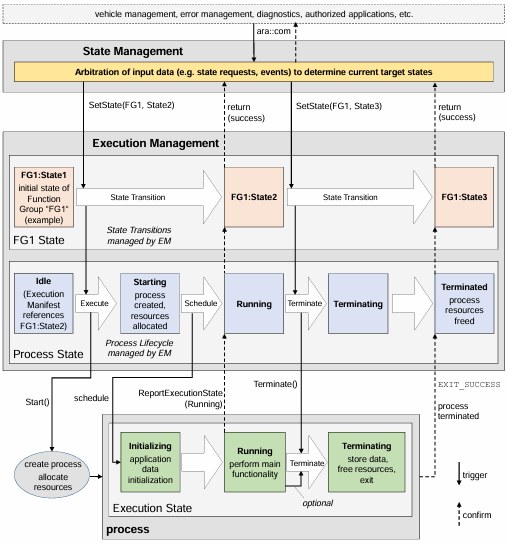
\includegraphics[width=0.9\textwidth]{Images/chapter2/em_stateinteraction.png}
%     \vspace{0.5cm}
%     \caption{State Interaction \cite{autosar_exec_mgmt}}
%     \label{fig:state_interaction}
% \end{figure}

% \paragraph*{Hierarchy of States:}
% To understand the interaction, one must first distinguish the three perspectives regarding "state" within the platform. {Function Group States (The Request)} are defined in the Manifest and controlled by State Management (SM). These represent a coherent mode of operation for a specific set of functionality (e.g., MachineFG in state Startup or a user-defined Function Group in state Run). SM determines what needs to run based on vehicle-wide events. {Process States (The Manager's View)} are maintained internally by Execution Management (EM). These track the lifecycle of a specific process instance (e.g., Idle, Starting, Running, Terminating, Terminated). EM uses these states to manage timeouts and resolve dependencies between applications. {Execution States (The Application's View)} are the internal lifecycle visible to the process itself (e.g., Initializing, Running, Terminating). The process reports these states to EM to confirm its readiness.

% \paragraph*{The Interaction Workflow:}
% The interaction is a cascading flow of triggers and confirmations. It typically begins with a request from State Management and ends with a confirmation from Execution Management, contingent upon the behavior of the individual processes.

% The process initiates with {The Trigger}, where State Management acts as the arbitrator. It analyzes input data (such as ignition signals or diagnostic requests) and determines that a Function Group (e.g., FG1) must transition to a specific state (e.g., State2). SM sends a \texttt{SetState(FG1, State2)} request to Execution Management. If FG1 is already in transition, EM will cancel the previous transition and reject the new request with \texttt{kCancelled} to ensure deterministic behavior.

% Upon receiving the request, Execution Management performs {Process Identification} by consulting the Execution Manifests to identify which processes are mapped to FG1:State2. Processes not currently running but required for State2 are queued for startup, while processes currently running but not required for State2 are queued for termination.

% For a process that needs to start, the {Startup and Initialization} phase begins. EM instructs the Operating System to create the process and allocate resources. Simultaneously, EM moves its internal tracking of the process to the Starting Process State. The OS creates the process entry point (\texttt{main}), and the process enters its own Execution State of Initializing. During this phase, the application loads configurations, initializes memory, and prepares to offer services.

% The critical point of interaction is {The Handshake}. EM considers the process to be Starting, but it does not assume the process is functional yet. Once the application completes its initialization and is ready to serve other components, it must explicitly call the API: \texttt{ara::exec::ExecutionClient::ReportExecutionState(kRunning)}. EM receives this call and updates its internal Process State from Starting to Running. If the process is a Non-reporting Process (legacy or simple applications), EM skips the handshake and assumes the process is Running immediately after the OS creates it.

% Finally, {Dependency Resolution and Confirmation} occurs. The interaction involves groups of processes; if Process B depends on Process A, EM will not start Process B until Process A has successfully performed the "Handshake" (reported \texttt{kRunning}). Only once all required processes for FG1:State2 have reported \texttt{kRunning} (and all unneeded processes have terminated), EM returns success to the original \texttt{SetState} call from State Management.

% \paragraph*{Deviations and Error Interactions:}
% The State Interaction mechanism is designed to be robust against failures. The interaction changes significantly if processes fail to participate correctly.

% In the case of a {Timeout on Startup}, if a process hangs during initialization and fails to call \texttt{ReportExecutionState(kRunning)} within a configured timeout, EM detects the timeout. EM attempts to restart the process up to a configured limit (\texttt{numberOfRestartAttempts}). If it still fails, EM aborts the Function Group transition, sets the state to Undefined, and reports an error to SM.

% An {Unexpected Termination} occurs if a process crashes (exits with a non-zero status) or exits without being asked (self-termination without permission) while EM thinks it should be running. EM detects the exit via OS mechanisms (e.g., \texttt{waitpid}) and reports this as an Unexpected Termination. The Function Group State is set to Undefined, and a callback is triggered in SM to handle the failure (e.g., by entering a Safe State).

% When transitioning out of a state, the {Termination Interaction} reverses. EM sends a \texttt{SIGTERM} signal to the process and updates the internal state to Terminating. The process receives the signal, saves data, cleans up resources, and exits with \texttt{EXIT\_SUCCESS}. EM detects the successful exit and moves the internal state to Terminated. If the process refuses to exit within a timeout, EM is authorized to use \texttt{SIGKILL} to enforce the state change.


% \paragraph*{Summary of Key Dependencies:}
% The State Interaction model relies on strict dependencies to ensure safety and determinism. {Manifest Verification} ensures EM will only execute processes explicitly mapped to the active Function Group State in the Manifest. The {Separation of Concerns} means the process does not know about the "Machine State" or "Function Group," only that it is Initializing or Running; EM acts as the bridge. Furthermore, there are {No Hidden Dependencies}: dependencies between processes must be resolved within the same Function Group State. A process in Group A cannot block a process in Group B via Execution Management mechanisms; such logic must be handled by State Management.

% By decoupling the request (SM) from the execution (EM) and the confirmation (Process), the Adaptive Platform ensures that the system state is always a verified reflection of the running software, rather than just a target configuration.


\subsubsection{State Interaction}

The operational behavior of the AUTOSAR Adaptive Platform relies on synchronizing three distinct state layers. This ``State Interaction'' ensures that the platform does not blindly start processes. Instead, it requires confirmation that applications are fully initialized and ready to run before declaring a state transition complete.

\begin{figure}[h]
    \centering
    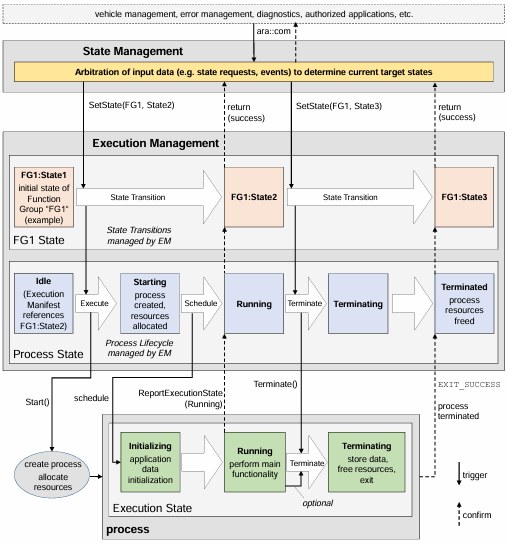
\includegraphics[width=0.9\textwidth]{Images/chapter2/em_stateinteraction.png}
    \vspace{0.5cm}
    \caption{State Interaction \cite{autosar_exec_mgmt}}
    \label{fig:state_interaction}
\end{figure}

\paragraph*{Understanding the Diagram Workflow:}
As illustrated in Figure \ref{fig:state_interaction}, the interaction between the layers acts as a clear chain of triggers (requests) and confirmations. To understand this, we must look at three distinct perspectives:

\begin{itemize}
    \item \textbf{State Management (The Requestor):} State Management (SM) acts as the arbitrator. Based on vehicle events, it decides the target state and triggers the workflow by sending a \texttt{SetState} request (e.g., \texttt{SetState(FG1, State2)}) to Execution Management.
    \item \textbf{Execution Management (The Manager):} Execution Management (EM) receives the request and manages the state transition. For processes that need to start, it moves its internal Process State from \texttt{Idle} to \texttt{Starting}. It then interacts with the Operating System to create the process and allocate resources.
    \item \textbf{The Process (The Application):} Once scheduled, the process enters its internal \texttt{Initializing} state to load data and set up services. Crucially, EM waits for a ``handshake.'' Once initialization is complete, the process explicitly sends a \texttt{ReportExecutionState(Running)} signal back to EM.
\end{itemize}

\paragraph*{Confirmation and Termination:}
After receiving this running confirmation, EM updates its internal state to \texttt{Running} and finally returns a ``success'' confirmation back to State Management, completing the startup workflow. 

The termination process follows a similar, reversed logic. When SM requests a new state that requires shutting down an application, EM sends a \texttt{Terminate()} trigger. The process enters the \texttt{Terminating} state to safely store data and free resources before exiting with an \texttt{EXIT\_SUCCESS} signal. EM then marks the process as \texttt{Terminated} and confirms the success with SM.

\paragraph*{Summary:}
Ultimately, this interaction model relies on strict rules and clear separation of responsibilities. By separating the request (from SM), the execution (by EM), and the confirmation (from the Process), the platform guarantees that the system's state accurately reflects the actual running software.


% \subsection{Communication Management (\texttt{ara::com})}

% Communication Management is responsible for all aspects of communication between applications in a distributed real-time embedded environment, acting as the middleware that abstracts network details from the application logic. It facilitates Service-Oriented Communication (SoC) by providing a standardized API that allows Adaptive Applications to offer or consume services without knowledge of the underlying transport mechanisms. ara::com establishes communication paths between partners at runtime, relying on the Service Registry to broker the connection between Service Providers and Service Consumers, whether they reside on the same machine or across the vehicle network.

% It manages the exchange of data through the Proxy/Skeleton architectural pattern, where the Service Skeleton connects the provider's implementation to the middleware, and the Service Proxy provides the consumer with a local C++ interface to access the remote service. For this system, ara::com utilizes the SOME/IP network binding to handle the specific requirements of the transport layer. This binding is responsible for discovering services on the network (Service Discovery) and serializing application data—specifically Methods, Events, and Fields—into the SOME/IP wire format. This separation of the Language Binding (C++ API) from the Network Binding ensures that the application code remains portable and independent of the specific protocol configuration defined in the Service Instance Manifests.

% To ensure secure and reliable operation, Communication Management enforces strict access control and data integrity. It integrates with Identity and Access Management (IAM) to verify that a requesting application process possesses the required Grants to access a specific Service Interface, dropping unauthorized requests at the middleware level. Furthermore, ara::com supports End-to-End (E2E) protection, which safeguards the transmission of events and methods against faults such as data corruption or loss, ensuring that safety-critical data exchanged via SOME/IP remains valid upon reception.

\subsection{Communication Management (\texttt{ara::com})}

Communication Management (\texttt{ara::com}) acts as the middleware that handles all communication between applications in a real-time embedded environment. It enables Service-Oriented Communication (SoC) by providing a standardized API, allowing applications to offer or consume services without needing to know the complex underlying network details. At runtime, it uses a Service Registry to connect Service Providers with Service Consumers across the vehicle network.

The system exchanges data using the Proxy/Skeleton pattern. The Service Skeleton connects the provider to the middleware, while the Service Proxy gives the consumer a local C++ interface to access remote services. To handle data transport, \texttt{ara::com} utilizes network bindings like SOME/IP and DDS (Data Distribution Service). These bindings manage service discovery and convert application data—such as Methods, Events, and Fields—into the appropriate network format. By separating the C++ language API from the network protocols, the application code remains flexible and easy to port.

Finally, \texttt{ara::com} ensures secure and reliable data transfer. It works with Identity and Access Management (IAM) to verify that applications have the correct permissions before allowing access to a service. Additionally, it supports End-to-End (E2E) protection to prevent data loss or corruption, guaranteeing that safety-critical information exchanged via SOME/IP or DDS remains accurate and secure.


\subsubsection{Block View Diagram}

\begin{figure}[h]
    \centering
    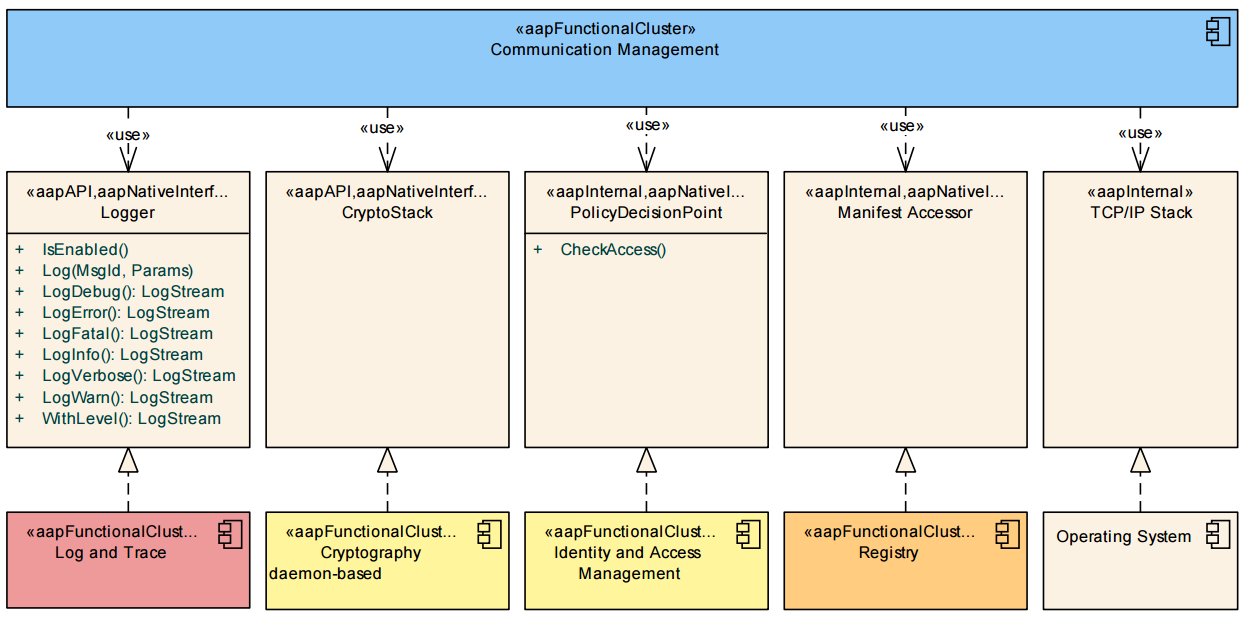
\includegraphics[width=1\textwidth]{Images/chapter2/com_required.png}
    \vspace{0.5cm}
    \caption{Required Interfaces of Communication Management \cite{autosar_sw_arch}}
    \label{fig:CommunicationManagementRequiredInterfaces}
\end{figure}

\textbf{Required Interfaces:} \begin{itemize} 
    \item \texttt{Cryptography::CryptoStack}: Communication Management shall use this interface to establish encrypted connections and generate / verify checksums (MAC).   
    \item \texttt{EventReporter}: This interface should be used to report security events. 
    \item \texttt{FVM}: Communication Management shall use this interface to get freshness values. 
    \item \texttt{Identity and Access Management::PolicyDecisionPoint}: Communication Management shall use this interface to check access to \texttt{ara::com} service methods, fields, and events. 
    \item \texttt{Log and Trace::Logger}: Communication Management shall use this interface to log standardized messages. 
    \item \texttt{Manifest Accessor}: Communication Management shall use this interface to read service information from the Manifests. 
    \item \texttt{Operating System::OperatingSystemInterface}: Communication Management should use this interface to create and control Threads used by the implementation. 
    \item \texttt{TCP/IP Stack}: Communication Management shall use this interface to establish and control TCP/IP-based network connections. 
\end{itemize}

\subsubsection{\texttt{ara::com} Responsibilities}

Communication Management (\texttt{ara::com}) is responsible for all aspects of communication between applications in a distributed, real-time embedded environment. Its primary design goal is to abstract the mechanisms used for finding and connecting communication partners, enabling developers to focus on application logic rather than data transport details. This cluster facilitates {Service-Oriented Communication (SOC)} between Adaptive Applications, handling both intra-machine (IPC) and inter-machine communication with other platforms, Classic AUTOSAR ECUs, or non-AUTOSAR entities.

To realize this, \texttt{ara::com} manages services defined by Events, Methods, and Fields using a {Service Registry}. This registry acts as a broker where applications register their Provided Services. Consuming applications utilize {Service Discovery} to locate these services at runtime. This allows for dynamic communication patterns where partners are identified during execution, though static configuration is also supported.

The architecture decouples software from transport technologies via two layers. The {Language Binding} maps abstract service definitions to specific C++ interfaces, generating Proxy classes for clients and Skeleton classes for providers to ensure type safety. The {Network Binding} handles data serialization for various protocols (e.g., SOME/IP, DDS, IPC) and manages transmission. This ensures application portability independent of the deployment scenario.

Beyond standard services, \texttt{ara::com} handles {Raw Binary Data Streams} for interacting with external sensors or systems providing untyped data. A dedicated API (\texttt{ara::com::raw}) allows applications to establish direct client/server connections over protocols like TCP/IP, bypassing the overhead of service serialization.

Finally, the module is critical for {Safety and Security}. It integrates End-to-End (E2E) protection to verify data integrity against communication faults. For security, it enforces access control by interacting with Identity and Access Management (IAM) to verify sender identity and permissions. Secure channels are managed using protocols like TLS, DTLS, and SecOC to ensure confidentiality and authenticity.

% \subsubsection{Service Registry and Discovery}

% In the Service-Oriented Communication (SOC) architecture of the AUTOSAR Adaptive Platform, the Service Registry and Service Discovery mechanisms are critical components that decouple application software from the underlying network topology.

% \paragraph*{The Service Registry:}
% The Service Registry functions as a central brokering instance within the \texttt{ara::com} infrastructure. Its primary responsibility is to maintain a dynamic directory of available services, abstracting the low-level details of network addresses and transport protocols from the application developers. When an Adaptive Application offers a service, it registers this service with the Service Registry, thereby making the functionality visible to other applications within the system. Conversely, when a client application requires a specific service, it does not connect to a hard-coded IP address; instead, it queries the Service Registry to locate the desired service instance. This abstraction allows the Communication Management logic to transparently route requests, whether the service resides in the same process, on the same machine, or on a remote ECU connected via Ethernet. In the physical architecture of the platform, the Registry is categorized under the Configuration functional clusters. It interacts internally with other clusters, such as Identity and Access Management and Communication Management, often utilizing the Manifest Accessor interface to validate service configurations against the system design.

% \paragraph*{The Service Discovery Process:}
% Service Discovery is the dynamic run-time process governed by \texttt{ara::com} to match Service Providers with Service Consumers based on the entries in the Service Registry. This mechanism allows the system to establish communication paths at runtime, supporting dynamic architectures where the availability of services may change or where the specific location of a service is not known at compile time. The discovery process begins with the Service Provider. When an application has initialized a service skeleton, it calls the \texttt{OfferService()} API. This action triggers the underlying network binding to announce the service's availability to the network. On the Service Consumer side, the application utilizes the \texttt{FindService()} or \texttt{StartFindService()} APIs. The \texttt{ara::com} runtime then queries the registry (or listens to network announcements) to find matching service instances. If matches are found, the runtime returns a list of handles (\texttt{ServiceHandleContainer}) to the consumer, which can then be used to instantiate a Proxy and begin data exchange.

% \begin{figure}[h]
%     \centering
%     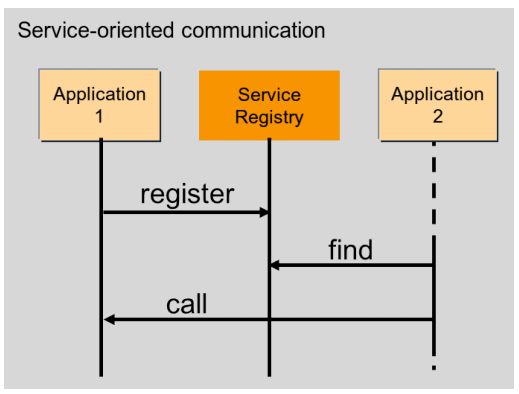
\includegraphics[width=0.5\textwidth]{Images/chapter2/com_soc.png}
%     \vspace{0.5cm}
%     \caption{Service-oriented communication \cite{autosar_com_mgmt}}
%     \label{fig:com_soc}
% \end{figure}

% \paragraph*{Protocol-Specific Implementation:}
% While the \texttt{ara::com} API abstracts the discovery process for the developer, the underlying behavior varies significantly depending on the network binding configuration.
% \begin{itemize}
%     \item \textbf{SOME/IP Service Discovery:} When using the SOME/IP binding, offering a service triggers the SOME/IP Service Discovery Protocol. This involves sending OfferService messages, which may be multicast or unicast depending on the configuration. The process includes configurable phases, such as an "Initial Wait Phase" and a "Repetition Phase," to ensure robust announcement on the network. Similarly, finding a service triggers FindService messages. The system also supports SubscribeEventgroup messages to manage dynamic subscriptions to specific data feeds within a service.

%     \item \textbf{SOME/IP Service Discovery:} When using the SOME/IP binding, offering a service triggers the SOME/IP Service Discovery Protocol. This involves sending OfferService messages, which may be multicast or unicast depending on the configuration. The process includes configurable phases, such as an "Initial Wait Phase" and a "Repetition Phase," to ensure robust announcement on the network. Similarly, finding a service triggers FindService messages. The system also supports SubscribeEventgroup messages to manage dynamic subscriptions to specific data feeds within a service.

%     \item \textbf{DDS Service Discovery:} The Data Distribution Service (DDS) binding offers two distinct discovery protocols configurable via the manifest. The first is {DomainParticipantUserDataQos}, which leverages the USER\_DATA QoS policy of DDS Domain Participants. The system encodes service IDs and instance IDs into the user data of the participant discovery messages. This approach is efficient as it uses the built-in DDS discovery traffic without creating extra entities. Alternatively, the system can use {Topic-Based Discovery}, employing a dedicated DDS Topic (e.g., \texttt{ara.com://services/discovery}) to publish service announcements. While this requires creating additional DataWriters and DataReaders, it enhances interoperability and supports advanced features like persistence and routing.

%     \item \textbf{Signal-Based Static Discovery:} For legacy compatibility or static configurations (e.g., interacting with simple sensors), the platform supports a static binding. In this case, \texttt{FindService} immediately returns a pre-configured handle containing static socket information (IP and Port) without performing active network discovery.
% \end{itemize}

% \paragraph*{Service Contract Versioning:}
% Service Discovery is not merely about finding a name; it also ensures compatibility. The platform supports Service Contract Versioning, where a service interface is defined by a Major and Minor version. During the discovery process, \texttt{ara::com} evaluates the version of the offered service against the version requested by the consumer. A connection is generally established only if the versions are backward-compatible (e.g., same Major version, offered Minor version greater than or equal to requested Minor version).

% \begin{figure}[h]
%     \centering
%     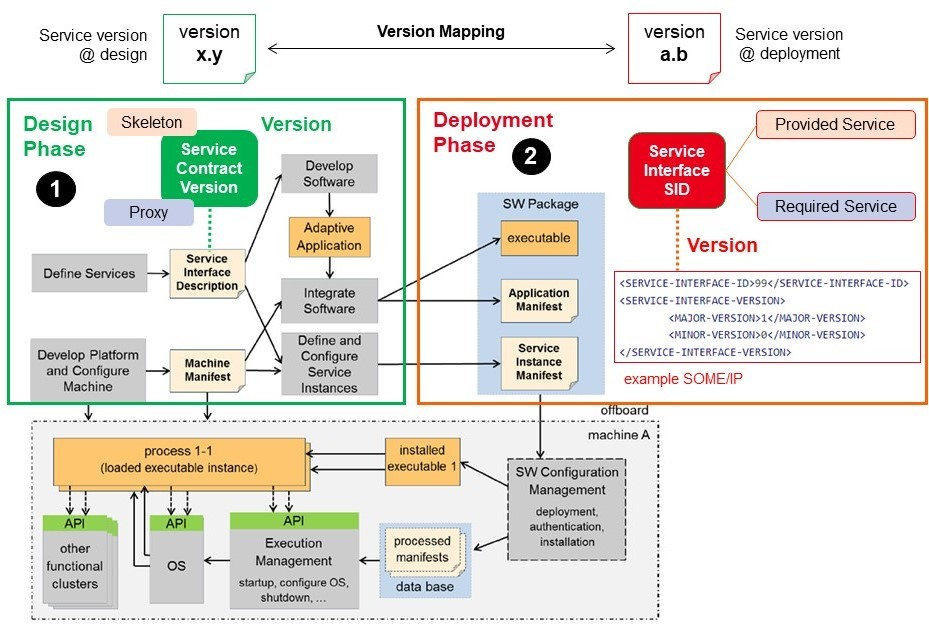
\includegraphics[width=0.9\textwidth]{Images/chapter2/com_servicecontract.jpg}
%     \vspace{0.5cm}
%     \caption{Service Contract Versioning flow \cite{autosar_com_mgmt}}
%     \label{fig:com_servicecontract}
% \end{figure}

\subsubsection{Service Registry and Discovery}

Within the \texttt{ara::com} Service-Oriented Communication (SOC) framework, the Service Registry and Service Discovery mechanisms decouple applications from the physical network topology. The Service Registry acts as a central broker, maintaining a dynamic directory of available services. This abstracts complex network addresses and transport protocols from developers, allowing the middleware to transparently route requests whether services reside locally or on a remote ECU. 

Service Discovery is the runtime process that matches Service Providers with Consumers. Providers register their capabilities via the \texttt{OfferService()} API, triggering network announcements. Conversely, consumers use the \texttt{FindService()} API to query the registry. Upon finding a match, the runtime returns a \texttt{ServiceHandleContainer}, which the consumer uses to instantiate a Proxy and initiate communication.

\begin{figure}[h]
    \centering
    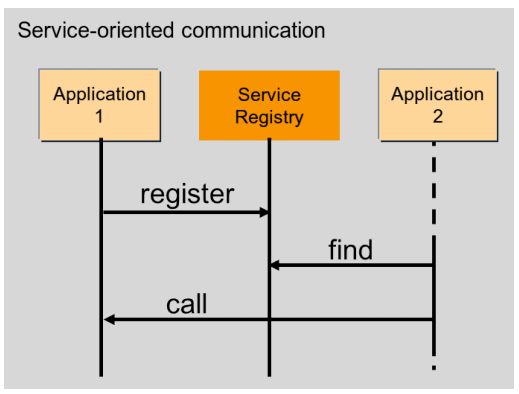
\includegraphics[width=0.5\textwidth]{Images/chapter2/com_soc.png}
    \vspace{0.5cm}
    \caption{Service-oriented communication \cite{autosar_com_mgmt}}
    \label{fig:com_soc}
\end{figure}

\paragraph*{Protocol-Specific Discovery \& Versioning:}
While the \texttt{ara::com} API abstracts the process, the underlying discovery mechanism varies by network binding:
\begin{itemize}
    \item \textbf{SOME/IP:} Triggers the SOME/IP Service Discovery Protocol, utilizing configurable \textit{OfferService} and \textit{FindService} multicast/unicast messages, alongside \textit{SubscribeEventgroup} for dynamic data feeds.
    \item \textbf{DDS:} Configurable via either \textit{DomainParticipantUserDataQos} (embedding service IDs efficiently into participant discovery traffic) or \textit{Topic-Based Discovery} (using a dedicated DDS topic for service announcements).
    \item \textbf{Static Discovery:} For legacy systems, \texttt{FindService} immediately returns a pre-configured static socket handle (IP/Port) without active network discovery.
\end{itemize}

Additionally, discovery enforces \textbf{Service Contract Versioning} (Major and Minor versions). A connection is successfully established only if the provider's version is backward-compatible with the consumer's request.

\begin{figure}[h]
    \centering
    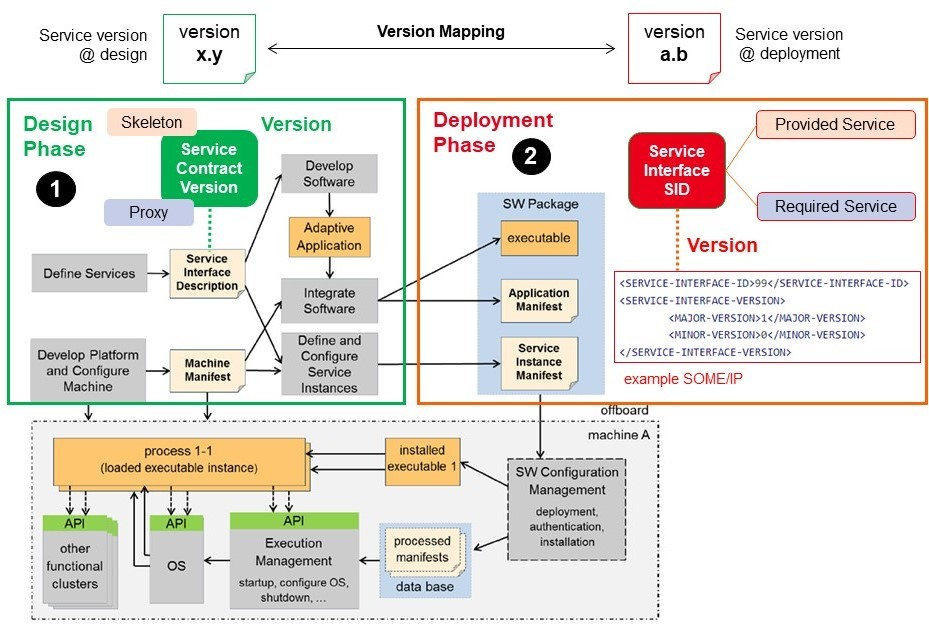
\includegraphics[width=0.9\textwidth]{Images/chapter2/com_servicecontract.jpg}
    \vspace{0.5cm}
    \caption{Service Contract Versioning flow \cite{autosar_com_mgmt}}
    \label{fig:com_servicecontract}
\end{figure}

% \subsubsection{Proxy/Skeleton Management}

% The Communication Management functional cluster in the AUTOSAR Adaptive Platform utilizes the Proxy/Skeleton design pattern to realize Service Oriented Communication. This architecture abstracts the underlying communication mechanisms, allowing applications to communicate regardless of whether the service resides in the same process, on a different process, or on a remote machine. The C++ Language Binding provides an object-oriented mapping of the services defined in the AUTOSAR meta-model, where a generator tool creates C++ classes containing type-safe representations of methods, events, and fields.

% On the client side, the {Service Proxy} acts as the local representative of a potentially remote service. These generated classes, known as Service Requester Proxies, can be used directly by the client application to access the service. To utilize a proxy, the client application must first identify a specific service instance using the \texttt{FindService} API, which returns handles that are passed to the proxy constructor to create a valid instance. The proxy provides mechanisms for calling service methods either synchronously, which blocks the caller until a result is returned, or asynchronously, where the function returns immediately and the result is retrieved later via \texttt{ara::core::Future}.

% On the server side, the {Service Skeleton} connects the user-provided service implementation to the middleware transport infrastructure. These generated classes are called Service Provider Skeletons and function as abstract base classes. A service implementation must derive from the generated skeleton class and implement the respective functionality. The skeleton provides specific methods to control the visibility of the service, such as \texttt{OfferService} to make the service available to applications and \texttt{StopOfferService} to stop offering it. Additionally, the architecture supports "Multi-Binding," allowing a single proxy or skeleton class to utilize different technical transport layers or protocols for communication.

% \begin{figure}[h]
%     \centering
%     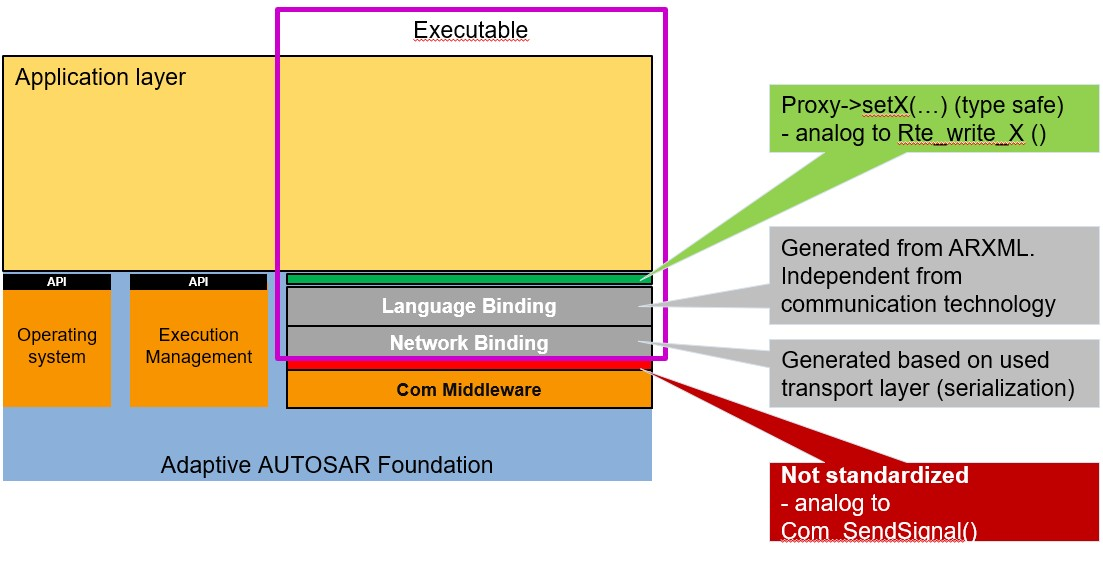
\includegraphics[width=1\textwidth]{Images/chapter2/com_networkbinding.jpg}
%     \vspace{0.5cm}
%     \caption{Example Language and Network Binding \cite{autosar_com_mgmt}}
%     \label{fig:com_languagebinding}
% \end{figure}

% The figure \ref{fig:com_languagebinding} illustrates the relationship between the Application layer (where Proxy calls occur), the generated Language Binding, and the Network Binding.

\subsubsection{Proxy/Skeleton Management}

The \texttt{ara::com} functional cluster uses the Proxy/Skeleton design pattern to enable Service-Oriented Communication. This architecture hides the underlying network details, allowing applications to communicate seamlessly, whether the service is on the same machine or across the network. A generator tool creates C++ classes that provide type-safe representations of methods, events, and fields based on the AUTOSAR meta-model.

\paragraph*{Service Skeleton (Provider):}
On the server side, the Service Skeleton connects the user's implementation to the middleware. The application creates an instance of the skeleton and calls \texttt{Start()} (or \texttt{OfferService()}) to make it available to others. When data needs to be sent, it triggers an event.

For example, a SOME/IP Provider might offer a sensor service like this:
\begin{lstlisting}[language=C++]
// SOME/IP Provider Initialization
m_Sensorv2 = std::make_unique<providersensor::rootswcomponent::port::Sensorv2>();
m_Sensorv2->Start(); // Offer service to the network

// Sending data via SOME/IP Event
m_Sensorv2->SendEventEvent_RequestDataTriggered(m_sensorData);
\end{lstlisting}

Similarly, a DDS Provider follows the exact same pattern, proving the abstraction of \texttt{ara::com}:
\begin{lstlisting}[language=C++]
// DDS Provider Initialization
m_PPort0 = std::make_unique<providersensor::aa::port::PPort0>();
m_PPort0->Start(); // Offer service over DDS

// Sending data via DDS Event
m_PPort0->SendEventimageDataEventTriggered(m_sensorData);
\end{lstlisting}

\paragraph*{Service Proxy (Client):}
On the client side, the Service Proxy acts as a local representative of the remote service. The client application uses the proxy to register handlers for incoming events or to call methods (synchronously or asynchronously).

For example, a SOME/IP Client registers a callback to handle incoming sensor data:
\begin{lstlisting}[language=C++]
// SOME/IP Client Registration
m_Sensorv2 = std::make_unique<clientsensor::rootswcomponent::port::Sensorv2>();
m_Sensorv2->RegistEventHandlerEvent_RequestData(
    [this](const sensor::transv2::proxy::events::Event_RequestData::SampleType& data) {
        // Handle received data
    }
);
m_Sensorv2->Start(); // Start listening
\end{lstlisting}

A DDS Client handles data similarly, registering an event handler for the specific DDS topic:
\begin{lstlisting}[language=C++]
// DDS Client Registration
m_RPort0 = std::make_unique<clientsensor::aa::port::RPort0>();
m_RPort0->RegistEventHandlerimageDataEvent(
    [this](const sensorCam::proxy::events::imageDataEvent::SampleType& data) {
        // Parse and process received image data
    }
);
m_RPort0->Start(); // Start listening
\end{lstlisting}

\paragraph*{Multi-Binding and Abstraction:}
As seen in the examples, whether the system uses SOME/IP or DDS, the application code structure remains nearly identical. This demonstrates the power of ``Multi-Binding,'' where a single proxy or skeleton class can utilize different network protocols without requiring changes to the core application logic. 

\begin{figure}[h]
    \centering
    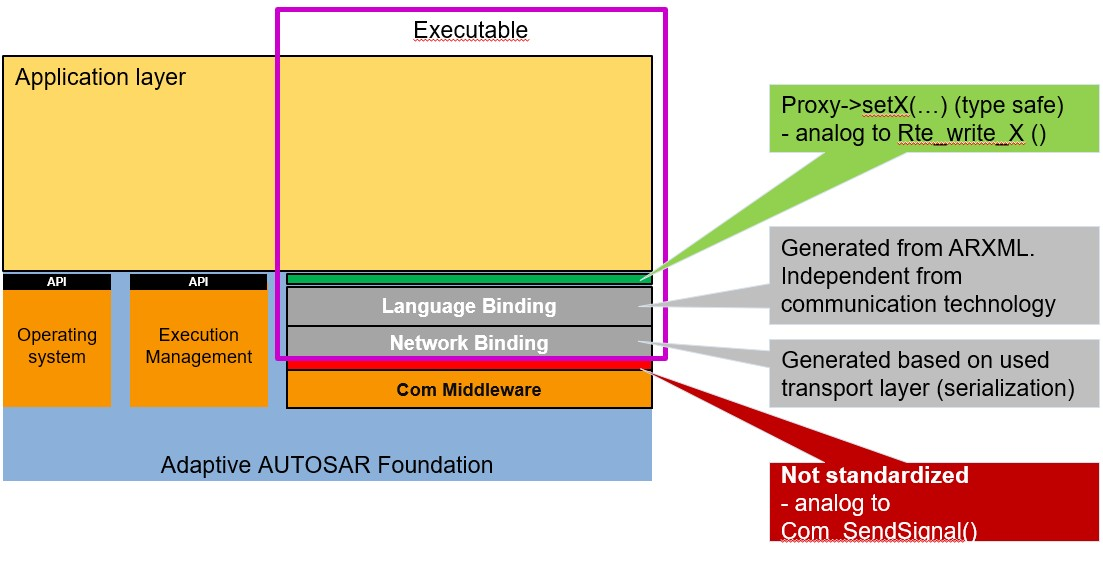
\includegraphics[width=1\textwidth]{Images/chapter2/com_networkbinding.jpg}
    \vspace{0.5cm}
    \caption{Example Language and Network Binding \cite{autosar_com_mgmt}}
    \label{fig:com_languagebinding}
\end{figure}

Figure \ref{fig:com_languagebinding} illustrates this relationship between the Application layer (where Proxy calls occur), the generated Language Binding, and the Network Binding.

\subsubsection{Access Control}

The access control mechanism within the Communication Management (\texttt{ara::com}) functional cluster is designed to restrict the interaction capabilities of both local applications and remote subjects, such as external ECUs, thereby limiting potential damage from compromised entities. This security feature integrates with the {Identity and Access Management (IAM)} framework, where \texttt{ara::com} acts as a {Policy Enforcement Point (PEP)} that queries the IAM {Policy Decision Point (PDP)} to authorize requests based on configured policies. Access permissions are modeled using \texttt{ComGrant} elements; if a grant references a \texttt{remoteSubject}, it applies to identified remote entities, otherwise, it applies to local processes based on their service instance to port prototype mappings. The enforcement of these rules is controlled by the \texttt{IamModuleInstantiation} configuration, which includes specific switches (\texttt{localComAccessControlEnabled} and \texttt{remoteAccessControlEnabled}) to independently activate access control for local processes and remote subjects.

For local applications, access control enforcement occurs at specific API interaction points. When an application attempts to offer a service via a \texttt{ServiceSkeleton} or find a service via a \texttt{ServiceProxy}, the framework checks for \texttt{ComOfferServiceGrant} or \texttt{ComFindServiceGrant} respectively; failure to possess these grants results in a \texttt{kGrantEnforcementError} returned to the application. Similarly, invoking service methods requires a \texttt{ComMethodGrant}, and unauthorized attempts will return a \texttt{kGrantEnforcementError} in the \texttt{Future} result of the method call. In contrast, unauthorized attempts to send or subscribe to events (requiring \texttt{ComEventGrant}) or triggers are handled by silently dropping the data or subscription request without notifying the application.

For remote access control, the system must first authenticate the remote subject using properties from established TLS connections, IPsec associations, or IP addresses before applying the modeled grants to permit or deny operations such as executing methods or subscribing to events.

\begin{figure}[h]
    \centering
    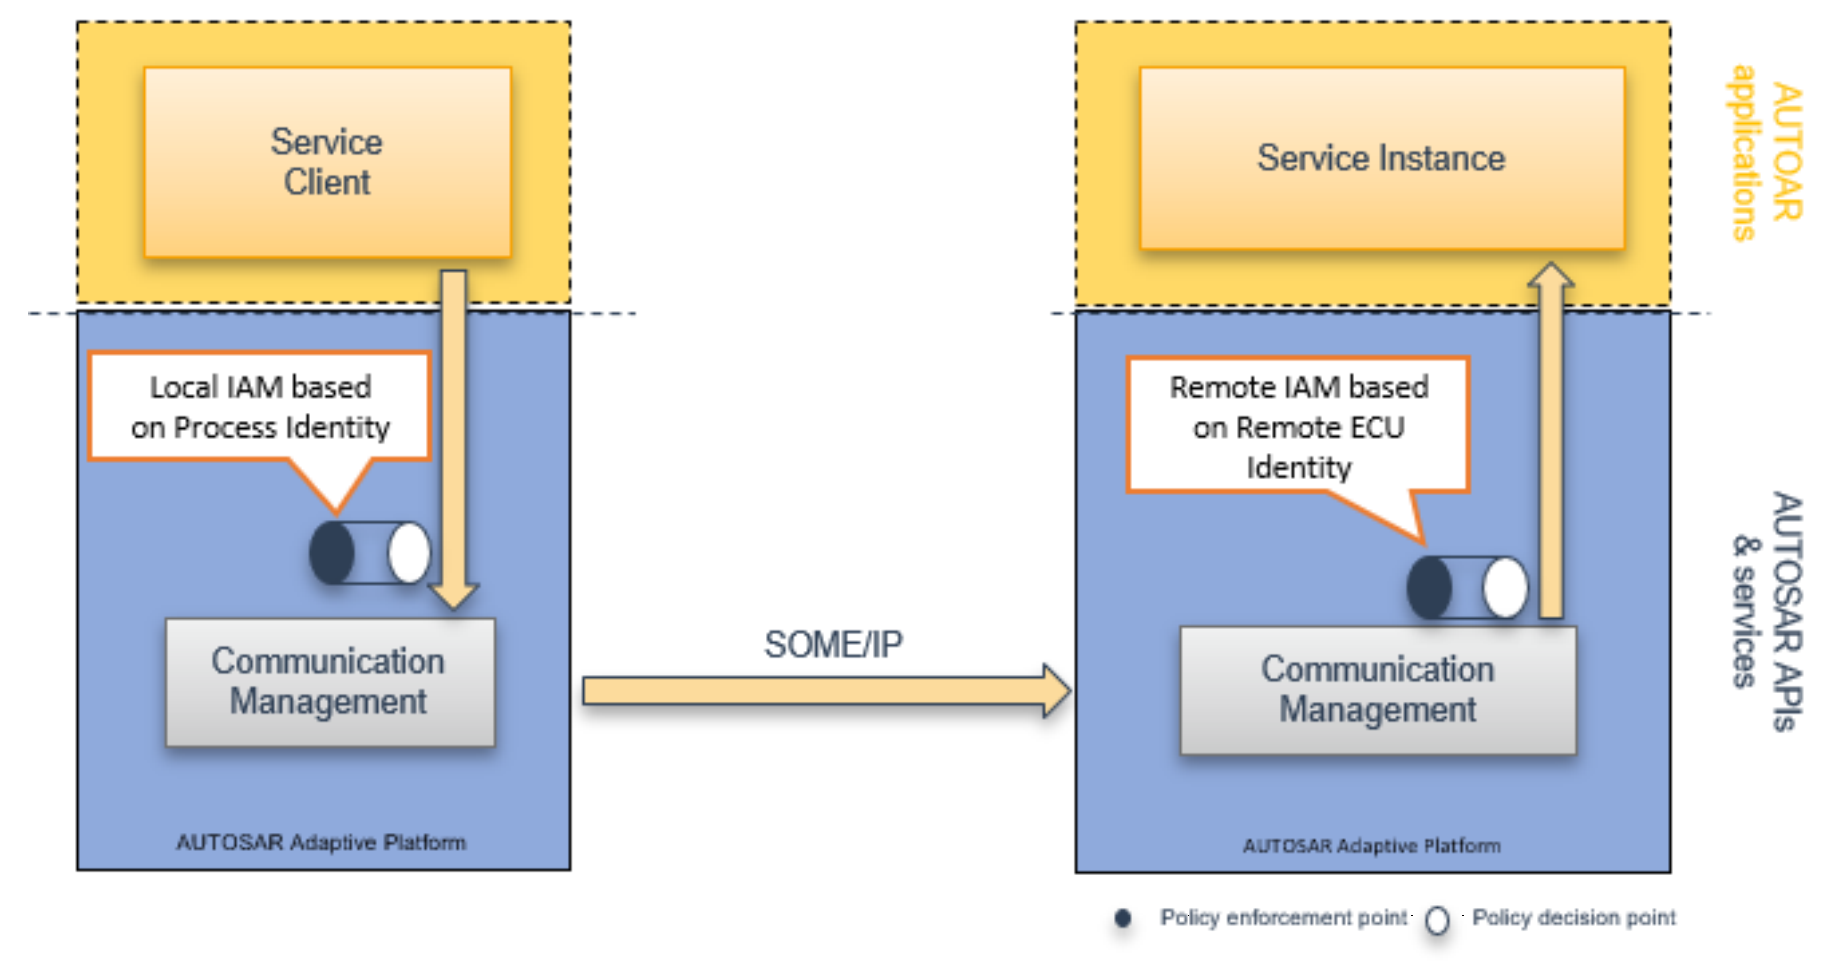
\includegraphics[width=1\textwidth]{Images/chapter2/com_iam.png}
    \vspace{0.5cm}
    \caption{Local and Remote Identity and Access Management \cite{autosar_com_mgmt}}
    \label{fig:com_iam}
\end{figure}



% \subsubsection{SOME/IP Protocol}

% See \ref{sec:someip_protocol} for more details.

% \subsection{Log and Trace (\texttt{ara::log})}

% The Log and Trace functional cluster (\texttt{ara::log}) is responsible for managing and instrumenting the logging features of the AUTOSAR Adaptive Platform, serving both development and production use cases. It provides standardized C++ interfaces that allow Adaptive Applications and other Functional Clusters to forward logging information to various ``sinks,'' such as a network communication bus, a file on the local file system, or a serial console. The module is designed to ensure platform stability by managing system resources and preventing data loss through internal buffering when high loads of trace information are generated simultaneously.

% To organize and filter the vast amount of data generated by modern vehicles, \texttt{ara::log} utilizes a strict identification and classification system. Every application instance is identified by a unique Application ID (\texttt{AppID}), while distinct logical groups within an application are distinguished using Context IDs (\texttt{CtxID}). Furthermore, every log message is assigned a specific severity level---ranging from \texttt{kFatal} and \texttt{kError} to \texttt{kDebug} and \texttt{kVerbose}. This allows the platform to be instrumented to only process and transmit messages above a configured threshold, enabling complex filtering and efficient fault detection without overloading the system.

% A critical architectural feature of \texttt{ara::log} is its support for two distinct classes of messages: Non-Modeled and Modeled. Non-Modeled messages (often called ``verbose'') contain all message arguments and text within the payload and are primarily used during development when flexibility is required. Conversely, Modeled messages (or ``non-verbose'') are optimized for production to minimize network bandwidth. In Modeled messages, static parts of the log (such as text strings) are stored in the application's ARXML manifest rather than being transmitted; only the message ID and dynamic arguments are sent over the network, allowing a viewer tool to reconstruct the full message using the model.

% Under the hood, \texttt{ara::log} relies on the standardized LT Protocol (Log and Trace Protocol) to pack logging information into a standardized delivery format, often utilizing the DLT (Diagnostic Log and Trace) backend implementation. This protocol is bus-agnostic and supports adding metadata, such as ECU IDs, to help clients sort and filter logs. Additionally, \texttt{ara::log} interacts with the Time Synchronization functional cluster (\texttt{ara::tsync}) to attach synchronized timestamps to messages, which is essential for correlating events across distributed systems.

% \begin{figure}[h]
%     \centering
%     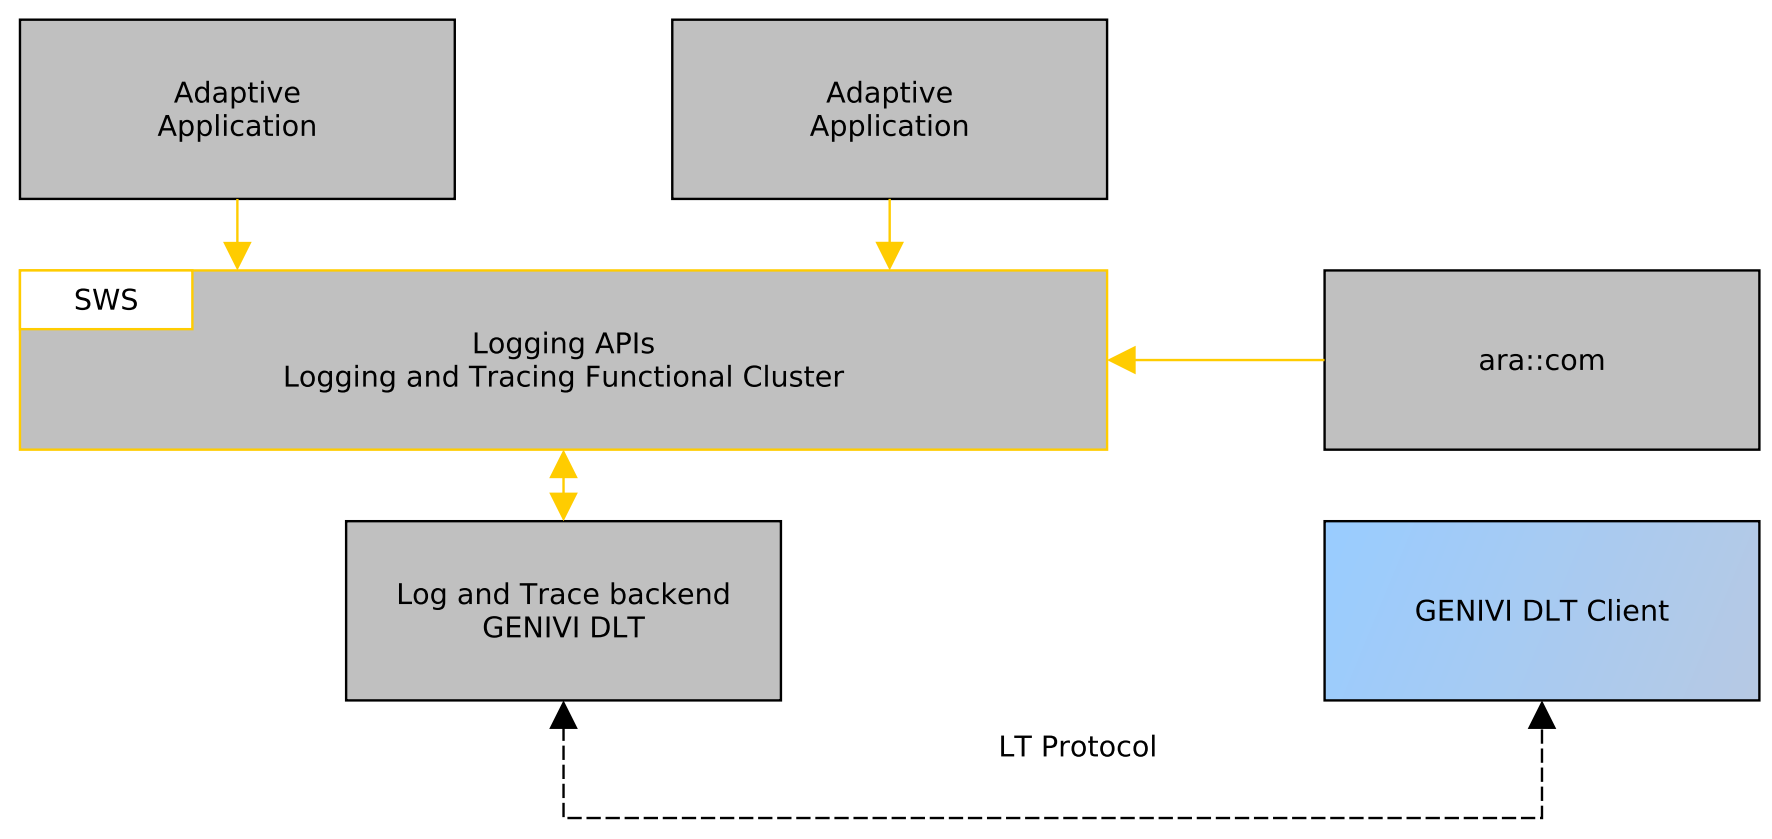
\includegraphics[width=1\textwidth]{Images/chapter2/log_arch.png}
%     \vspace{0.5cm}
%     \caption{Log and Trace Overview \cite{autosar_log_trace}}
%     \label{fig:log_arch}
% \end{figure}



% \subsubsection{Log Severity Levels}

% In the AUTOSAR Adaptive Platform, the Log and Trace functional cluster (\texttt{ara::log}) employs a standardized classification system known as ``severity levels'' to categorize every log message based on its importance. These levels are defined within the \texttt{ara::log::LogLevel} enumeration (based on \texttt{std::uint8\_t}) and serve a critical role in system stability by acting as a reporting filter. Each application process or logging context is configured with a specific log level threshold; the Logging framework only processes and transmits messages that have a severity equal to or higher than this configured threshold, while ignoring lower-priority messages. This filtering mechanism preserves CPU and memory resources by preventing the system from preparing and storing excessive data, such as verbose debug information, during normal production operation.

% \paragraph*{Defined Severity Levels:}
% The standard defines a specific hierarchy of severity levels, ranging from \texttt{0x00} to \texttt{0x06}, to cover various operational and development scenarios:

% \begin{table}[h]
%     \centering
%     \renewcommand{\arraystretch}{1.2}
%     \begin{tabular}{|l|c|p{9.5cm}|}
%         \hline
%         \textbf{Level Name} & \textbf{Value} & \textbf{Description} \\
%         \hline
%         \texttt{kOff} & \texttt{0x00} & This level indicates ``No logging'' and is used to disable log output entirely for a specific context or application. \\
%         \hline
%         \texttt{kFatal} & \texttt{0x01} & Represents a fatal error that is not recoverable. \\
%         \hline
%         \texttt{kError} & \texttt{0x02} & Denotes an error that has an impact on the correct functionality of the system. \\
%         \hline
%         \texttt{kWarn} & \texttt{0x03} & Used for warnings where correct behavior cannot be explicitly ensured. \\
%         \hline
%         \texttt{kInfo} & \texttt{0x04} & Provides high-level informational messages to understand the system flow. \\
%         \hline
%         \texttt{kDebug} & \texttt{0x05} & Contains detailed information intended specifically for programmers during development. \\
%         \hline
%         \texttt{kVerbose} & \texttt{0x06} & Represents the highest grade of information, providing extra-verbose debug messages. \\
%         \hline
%     \end{tabular}
%     \caption{Defined Log Severity Levels}
%     \label{tab:log_severity_levels}
% \end{table}

% \paragraph*{API Usage and Configuration:}
% To facilitate ease of use, the \texttt{ara::log::Logger} class provides dedicated API methods corresponding to each severity level, including \texttt{LogFatal()}, \texttt{LogError()}, \texttt{LogWarn()}, \texttt{LogInfo()}, \texttt{LogDebug()}, and \texttt{LogVerbose()}. Each of these methods returns a \texttt{LogStream} object pre-configured with the respective severity. Alternatively, if the severity needs to be determined programmatically at runtime, developers can use the \texttt{WithLevel()} method to pass the \texttt{LogLevel} as a parameter. To further optimize performance, the \texttt{IsEnabled()} function allows applications to check if a specific level is currently active before executing complex code to prepare log arguments, ensuring that resources are not wasted on messages that will eventually be discarded. The default log level is initially defined in the application execution manifest but can be overridden per context and adjusted dynamically at runtime via external tools.

% \subsubsection{Log Sinks and Output Bindings:}

% In the AUTOSAR Adaptive Platform, the Log and Trace functional cluster decouples the logging API used by applications from the physical destination of the log data. These destinations are referred to as Log Sinks, and the specific method of formatting and delivering data to them is known as an Output Binding. The selection of a sink depends on the configuration provided by the system integrator in the Machine Manifest, specifically through the \texttt{DltLogSink} meta-class, which defines the ``Log Mode'' or category of the sink. The primary supported output bindings allow logging to the console, a file on the local system, or a remote target via a network communication bus.

% \paragraph*{Console Output Binding:}
% The Console Binding, identified by the category \texttt{DLT\_LOGSINK\_CONSOLE}, directs log messages to the system's console output. While general layout aspects like timestamp formatting are implementation-defined, the specification mandates specific formatting rules to ensure consistency. The logging framework must append an End-Of-Line (EOL) sequence to every message. When a message contains multiple payload arguments, they are separated by a single space character. If an argument is annotated with attributes such as a name or a unit, these are displayed using colons as separators (e.g., \texttt{name:value:unit}). Specific data types have standardized representations: boolean values are output as ``0'' for false or ``1'' for true, raw binary data is rendered as a sequence of hexadecimal octets separated by apostrophes (e.g., \texttt{48'65'6c'6f}), and time durations are printed as decimal integers followed by their SI unit notation (e.g., \texttt{42ns}).

% \paragraph*{File Output Binding:}
% The File Binding is configured using the category \texttt{DLT\_LOGSINK\_FILE} and is used to store log messages persistently on the machine's non-volatile storage. This configuration requires a destination directory path defined in the \texttt{path} attribute of the \texttt{DltLogSink} configuration. Unlike the console binding, the specific visual appearance and formatting of the log file content are implementation-defined. It is explicitly noted that logging to a file is provided primarily for development, integration, and prototyping purposes and is generally not suitable for production environments.

% \paragraph*{Network (DLT) Binding:}
% The Network Binding, configured via \texttt{DLT\_LOGSINK\_NETWORK} or \texttt{DLT\_LOGSINK\_DLT}, represents a ``remote'' backend that forwards messages to a logging client (such as a DLT Viewer) over a communication bus, typically Ethernet. This binding utilizes the standardized Log and Trace (LT) protocol (often implemented via the DLT daemon) to pack information into a standardized delivery format. This mode supports extensive configuration, including specific Ethernet endpoint configurations (IP addresses and ports) and bandwidth monitoring to prevent data loss during high load. In this binding, C++ data types from the application are mapped to specific DLT payload types: strings (\texttt{const char*} or \texttt{StringView}) are output as \texttt{STRG} with UTF-8 encoding, raw binary data maps to \texttt{RAWD}, and booleans map to \texttt{BOOL}. Additionally, the log levels defined in the \texttt{ara::log} API have a 1:1 mapping to the log levels defined in the LT protocol.

% \paragraph*{Configuration and Architecture:}
% The configuration of these sinks is centralized in the Machine Manifest. The \texttt{DltLogSink} element allows the integrator to define the default log threshold, whether output buffering is used (specifically for console output), and the size of the message queue. The overall architecture allows for flexible instrumentation where the logging information provided by Adaptive Applications is forwarded to these configured sinks transparently, ensuring that the application code remains independent of the specific logging backend or destination.

% \paragraph*{Log Mode Configuration:}
% The following image illustrates how the Log Mode and Sink configurations are structured within the manifest, showing the relationship between the \texttt{DltLogSink} and the Ethernet endpoint configuration for network logging.

% \begin{figure}[h]
%     \centering
%     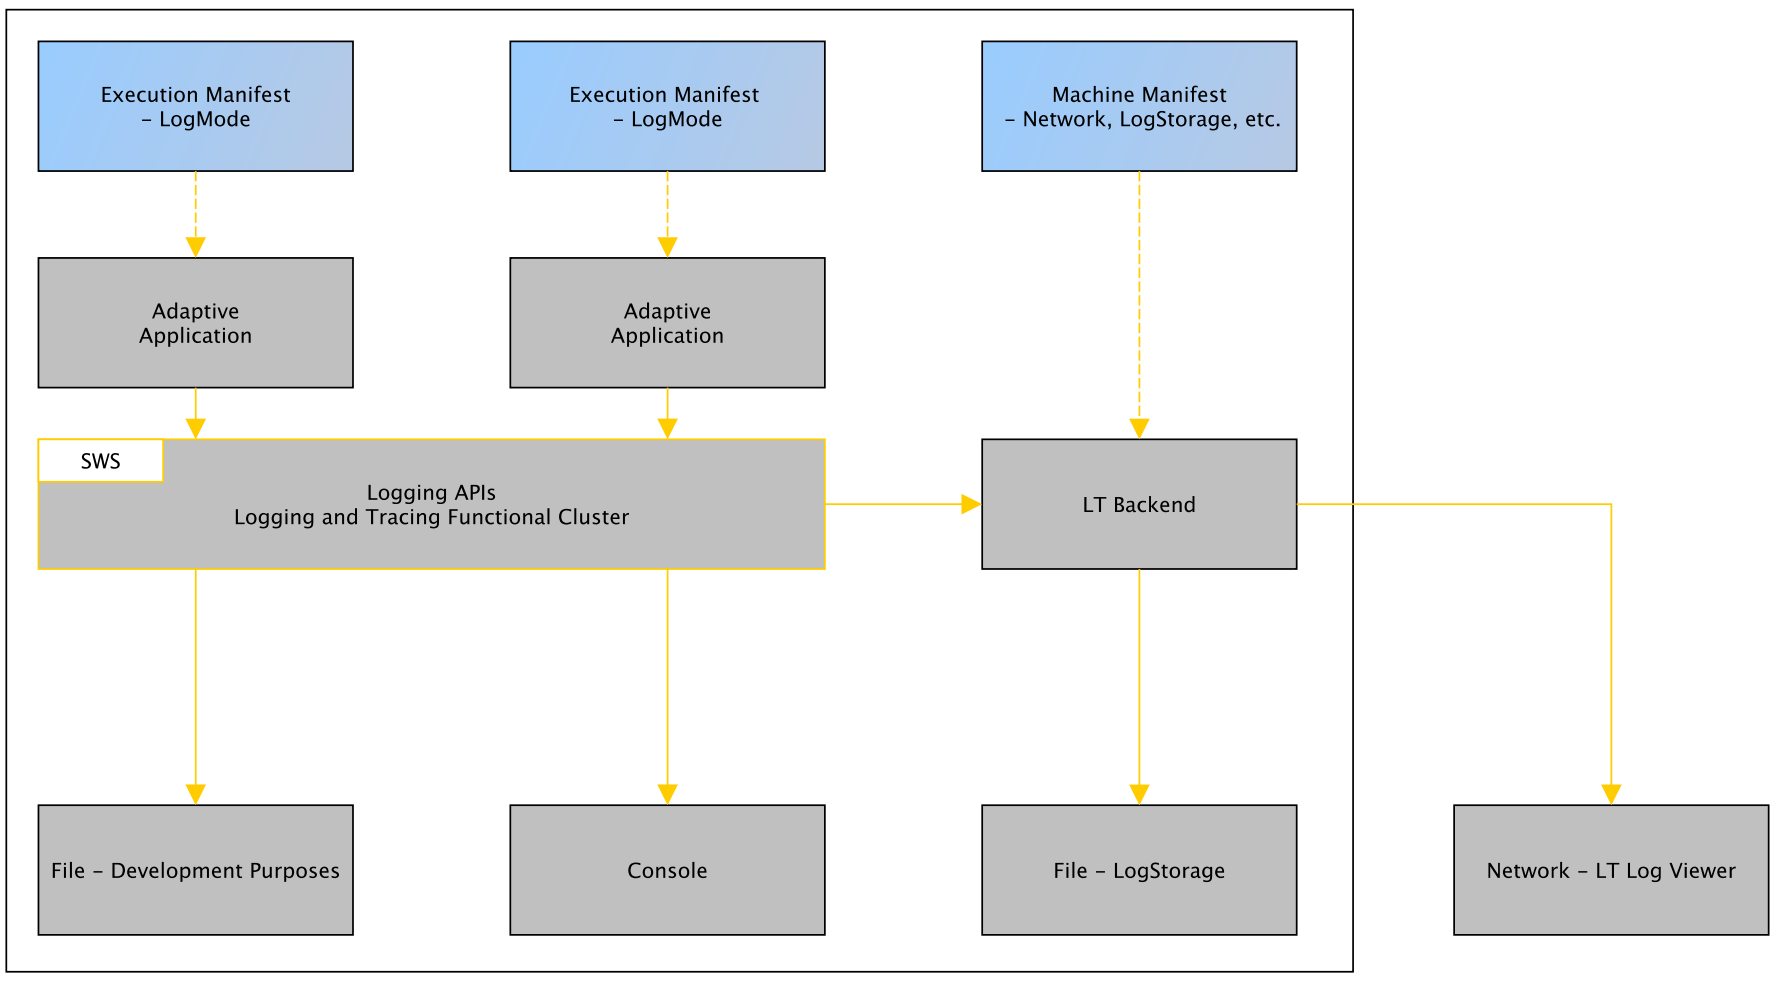
\includegraphics[width=1\textwidth]{Images/chapter2/log_mode.png}
%     \vspace{0.5cm}
%     \caption{Log Mode \cite{autosar_log_trace}}
%     \label{fig:log_mode}
% \end{figure}

% \subsubsection{Logging Contexts and Application IDs:}

% To effectively manage and distinguish logging data across a distributed system, the AUTOSAR Adaptive Platform utilizes a hierarchical identification scheme consisting of Application IDs and Logging Contexts.

% \paragraph*{Application IDs:}
% To distinguish the logs of different application instances within a system, every Application process must be assigned a specific Application ID. This identifier serves as a string value that associates generated logging information with its specific originating user application. While uniqueness across different ECUs is not required (as the ECU ID acts as a differentiator), the system integrator bears the responsibility of ensuring that each Application process instance within a single ECU possesses a unique Application ID. This configuration is typically supplied through the application execution manifest, which allows integrators to perform consistency checks. Because the Application ID string might be short or cryptic due to implementation limits, an optional Application Description can be provided as descriptive text to further identify the application instance.

% \paragraph*{Logging Contexts:}
% To allow for finer granularity within a single Application process, the platform uses Logging Contexts to distinguish logs from different logical groups or internal functional units. Each context is defined by a Context ID, which is a string identifier that must be unique within the scope of that specific Application process. Unlike the Application ID, the Context ID is assigned by the developer and is not modeled in the manifest. This structure is particularly important for software libraries running within an application's scope; they should reserve their own Context IDs to differentiate their internal logs from those of the parent application or other libraries. Similar to the application level, a Context Description string must be provided to offer a human-readable explanation of the context.

% \paragraph*{Initialization and Usage:}
% The connection between these identifiers is established when the application initializes the logging framework. An application process creates a logger instance for a specific context by calling the \texttt{ara::log::CreateLogger} function, passing the specific Context ID, Context Description, and optionally a default log level. This function creates a logger context instance internally within the Logging framework and returns a reference to the application, ensuring the context is registered against the back-end. Consequently, all log messages generated through this logger instance are tagged with both the Application ID (derived from the manifest) and the specific Context ID, allowing for precise filtering and analysis.

% \paragraph*{Architecture Overview:}
% The Figure \ref{fig:log_arch} above illustrates the high-level architecture where these logging contexts operate, showing the interaction between the Adaptive Application and the Logging Functional Cluster


\subsection{Log and Trace (\texttt{ara::log})}

The Log and Trace functional cluster (\texttt{ara::log}) provides a standardized C++ interface for Adaptive Applications to forward diagnostic and trace information to various output destinations (sinks). It is designed to maintain platform stability by managing system resources and buffering data during high-load scenarios. To efficiently organize the vast amount of vehicle data, \texttt{ara::log} employs a strict hierarchical identification system and severity-based filtering mechanisms.

\begin{figure}[h]
    \centering
    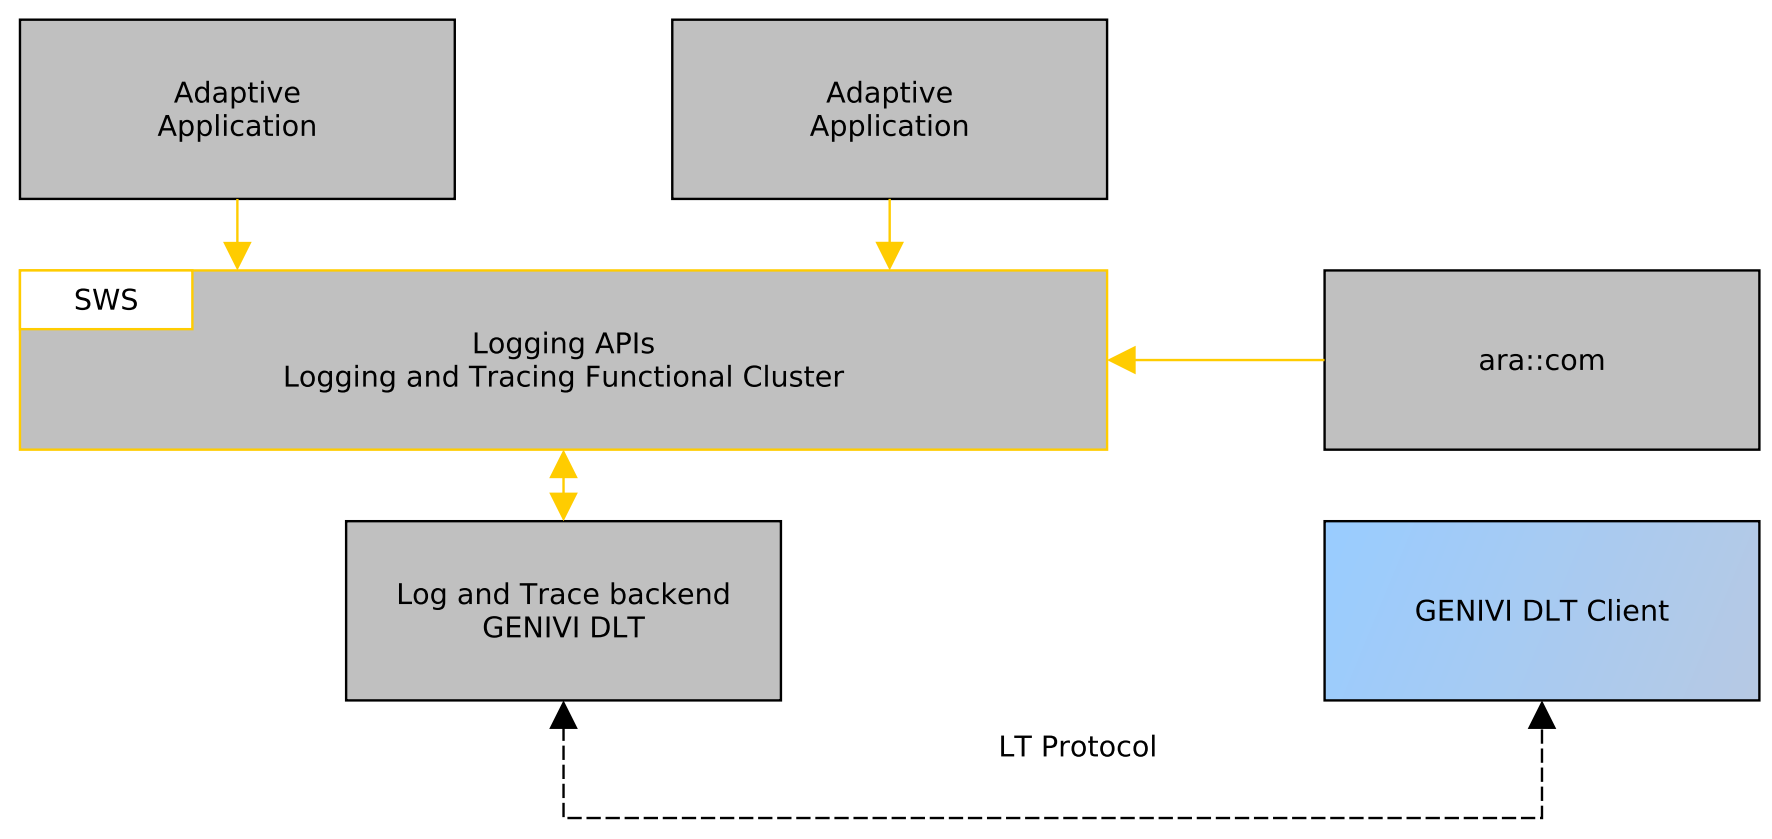
\includegraphics[width=0.9\textwidth]{Images/chapter2/log_arch.png}
    \vspace{0.5cm}
    \caption{Log and Trace Overview \cite{autosar_log_trace}}
    \label{fig:log_arch}
\end{figure}

\subsubsection{Severity Levels and Filtering}
To prevent resource exhaustion, \texttt{ara::log} categorizes messages using predefined severity levels, ranging from \texttt{kFatal} (0x01) and \texttt{kError} (0x02) to \texttt{kDebug} (0x05) and \texttt{kVerbose} (0x06). Applications are configured with a specific severity threshold; the framework only processes and transmits messages that meet or exceed this limit. This dynamic filtering ensures that excessive debug information is discarded during normal production operation, thereby conserving CPU and network bandwidth. Developers can easily generate logs using dedicated API methods such as \texttt{LogInfo()} or \texttt{LogError()}, which return a pre-configured \texttt{LogStream} object.

\subsubsection{Log Sinks and Output Bindings}
The framework decouples the logging API from the physical data destinations, known as Log Sinks. The routing behavior is configured within the Machine Manifest via the \texttt{DltLogSink} meta-class. The primary output bindings include:
\begin{itemize}
    \item \textbf{Console Binding:} Directs formatted messages to the standard console output, utilizing specific rules for separating arguments and rendering raw data.
    \item \textbf{File Binding:} Stores logs persistently on non-volatile storage, primarily utilized for development and integration testing.
    \item \textbf{Network (DLT) Binding:} Forwards messages over an Ethernet bus to a remote client (e.g., a DLT Viewer) using the standardized Log and Trace (LT) protocol. This mode supports bandwidth monitoring and maps C++ data types to specific DLT payloads.
\end{itemize}

\begin{figure}[h]
    \centering
    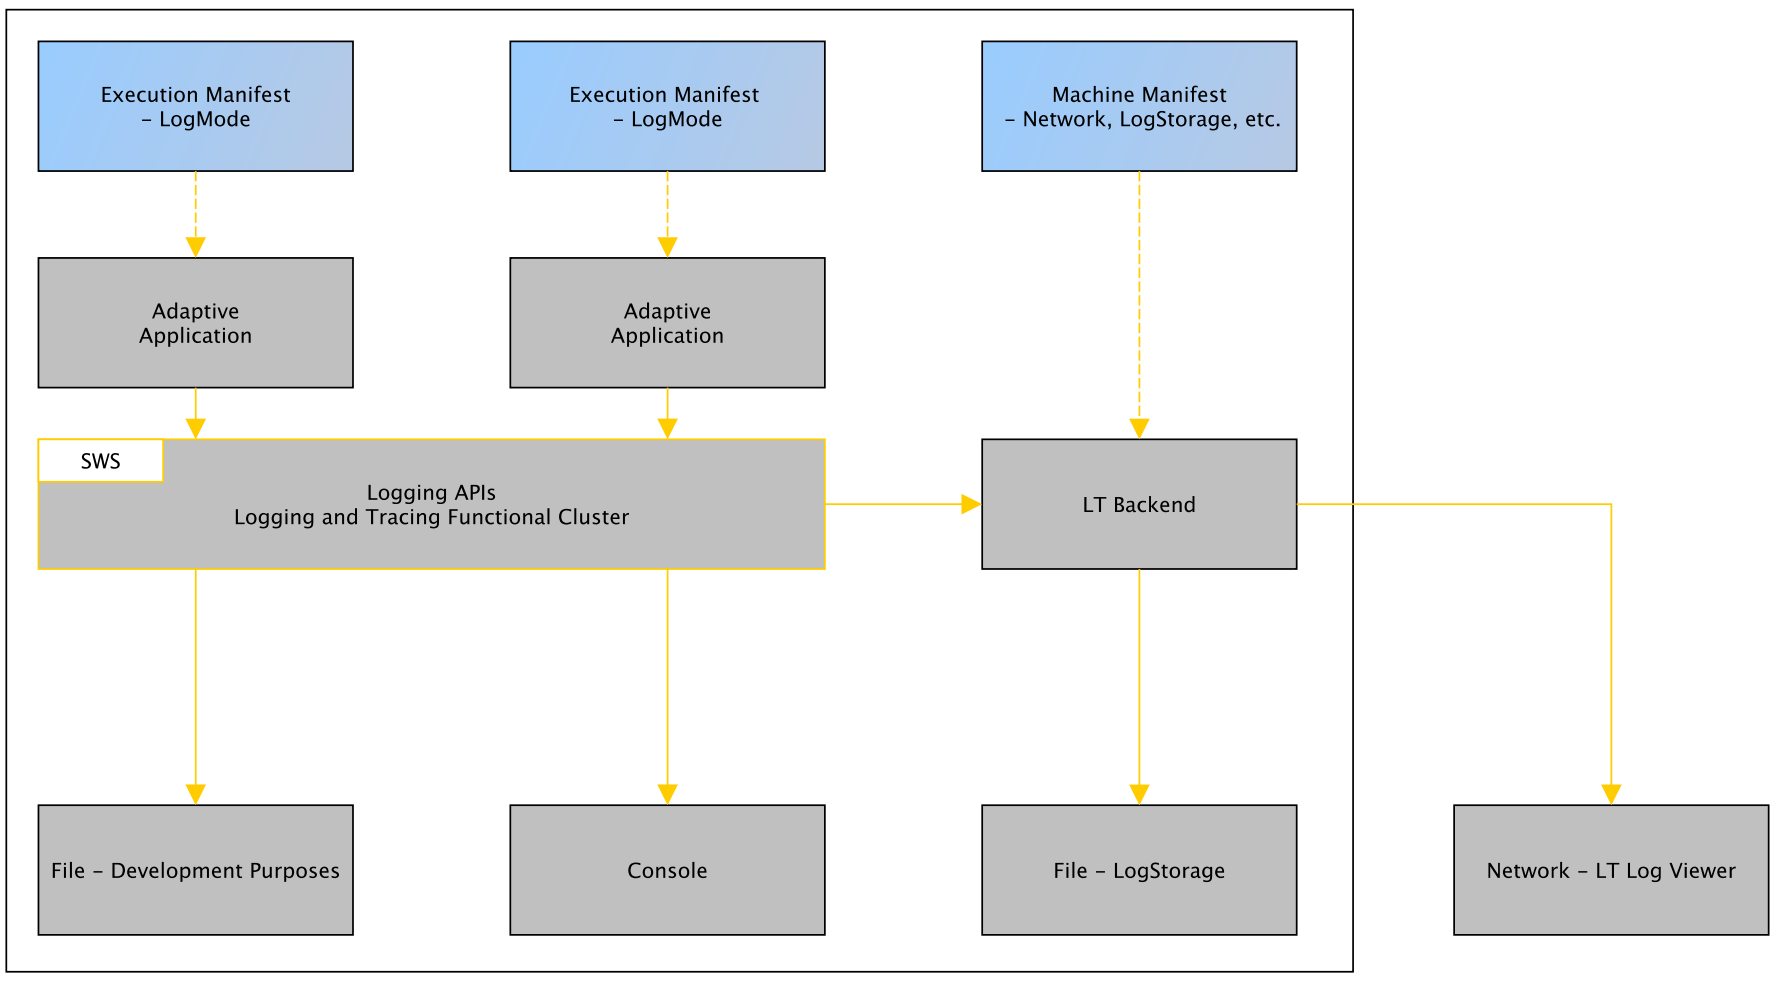
\includegraphics[width=0.9\textwidth]{Images/chapter2/log_mode.png}
    \vspace{0.5cm}
    \caption{Log Mode Configuration \cite{autosar_log_trace}}
    \label{fig:log_mode}
\end{figure}

\subsubsection{Application and Context Identification}
To track the origin of log messages across a distributed system, \texttt{ara::log} assigns a unique {Application ID} to every process instance, typically defined in the execution manifest. For finer granularity, developers define {Context IDs} to distinguish logs from different logical functional units or libraries within the same application. When an application calls \texttt{ara::log::CreateLogger}, it binds the specific Context ID to the logger instance. Consequently, all generated messages are tagged with both the Application ID and Context ID, enabling precise sorting and fault tracing on the backend.

\section{Development Toolchains}
PopcornSAR is a specialized Software-Defined Vehicle (SDV) tool and platform vendor focusing on the AUTOSAR Adaptive Platform to support automotive projects through advanced tools and engineering services. Their core design tool, {AutoSAR.io}, serves as a comprehensive authoring environment for modeling and configuring both Adaptive and Classic AUTOSAR platforms, offering features like graphical modeling, code generation, and interoperability with formats such as CAN DBC and COVESA VSS. This is complemented by {PARA}, an independently developed software framework designed for High-Performance Computing (HPC) that provides essential Adaptive AUTOSAR Functional Clusters---including communication (\texttt{ara::com}), execution management (\texttt{ara::exec}), and functional safety (\texttt{ara::phm})---to enable flexible and secure vehicle system development.

\begin{figure}[h]
    \centering
    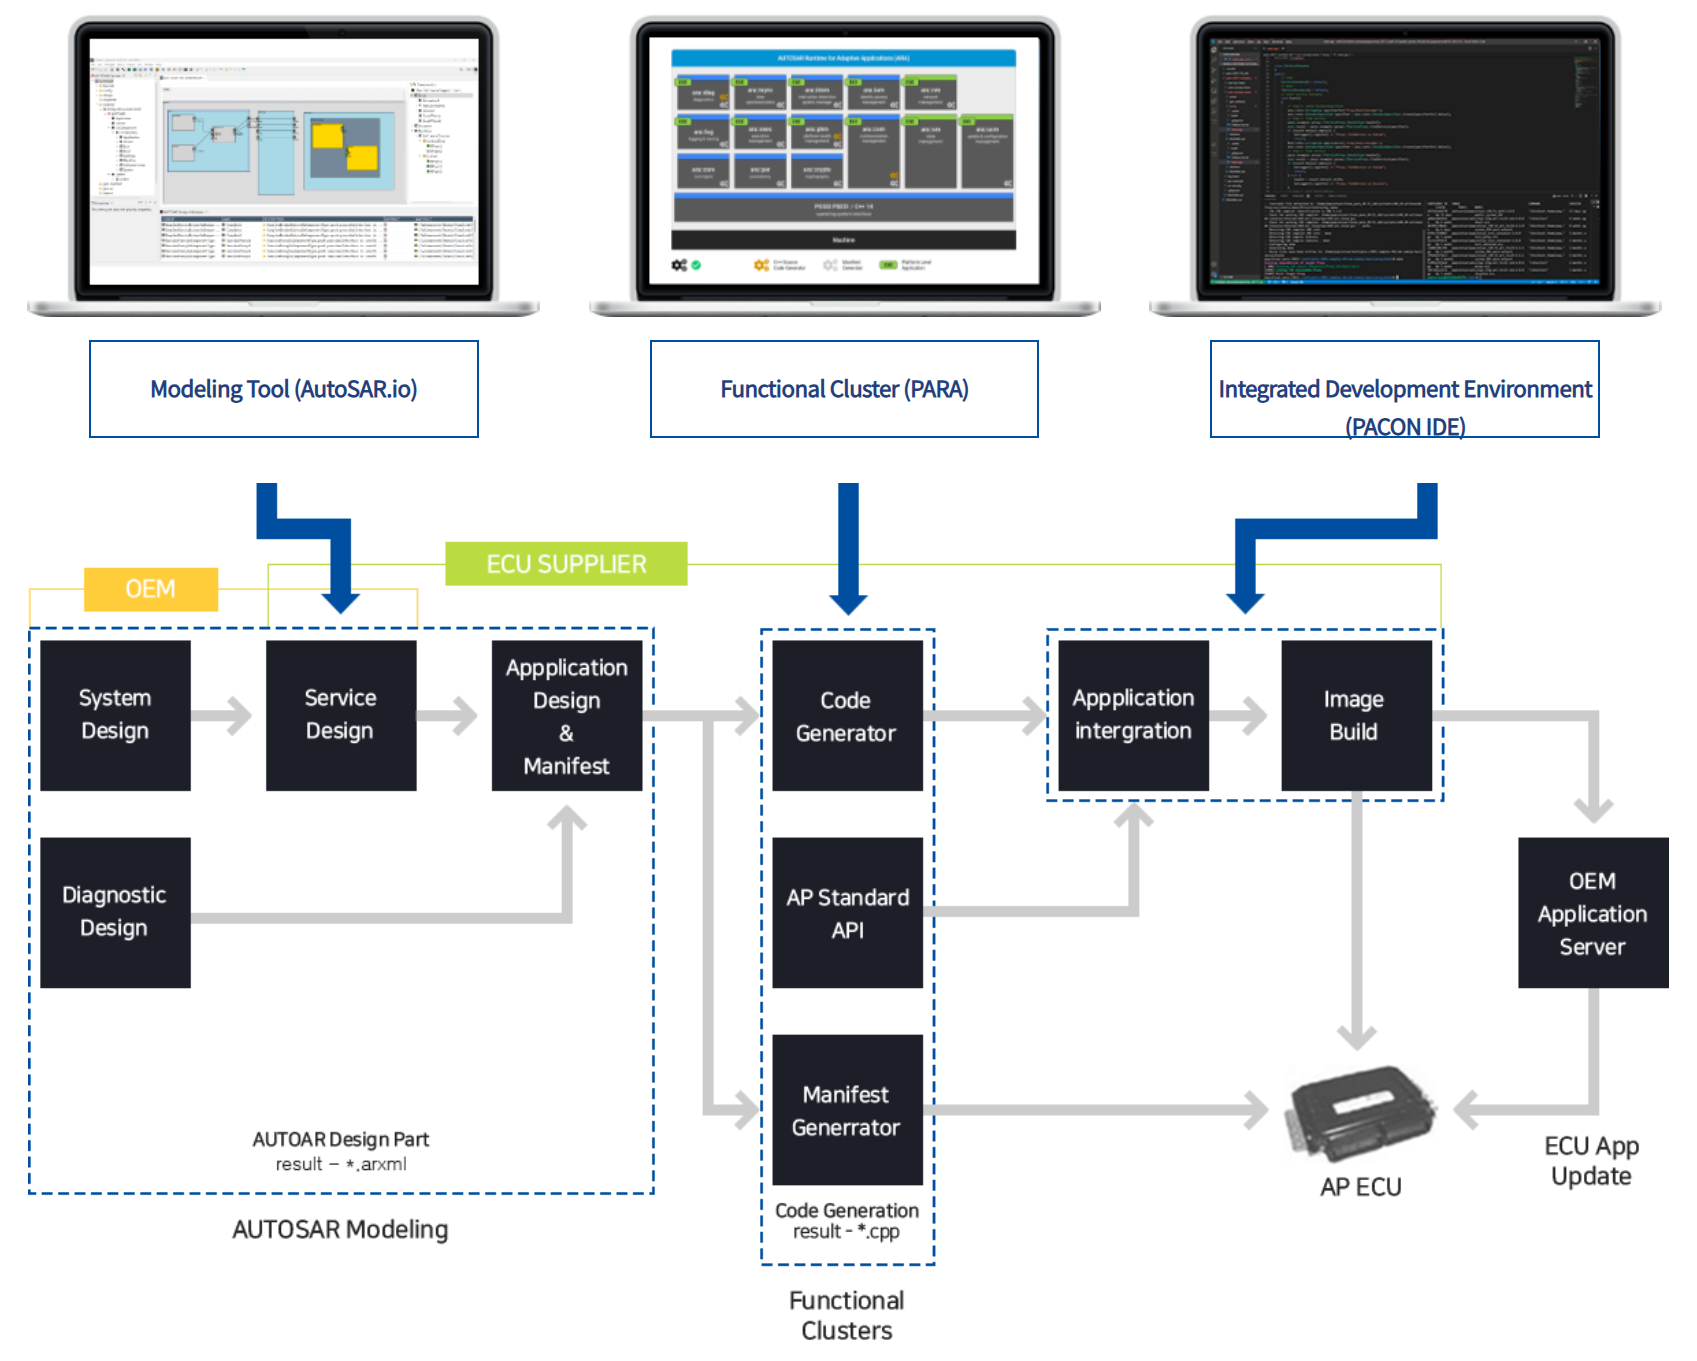
\includegraphics[width=1\textwidth]{Images/chapter2/tool_breakdowntool.png}
    \vspace{0.5cm}
    \caption{PopcornSAR Toolchain Breakdown \cite{popcornsar_intro}}
    \label{fig:popcornsar_toolchain}
\end{figure}

\subsection{AutoSAR.io}

AutoSAR.io is a powerful authoring tool developed by PopcornSAR, designed for the modeling and configuration of AUTOSAR projects within automotive systems. It serves as a comprehensive, future-proof development environment that supports the entire engineering spectrum, including System Architecture as well as both the Adaptive and Classic AUTOSAR Platforms. The tool is specifically built to empower customers in the efficient development of Software-Defined Vehicles (SDV), enabling them to significantly reduce complexity and accelerate the advancement of future automotive architectures.

Key features of AutoSAR.io include the capability to handle AUTOSAR System Design and the implementation of both Adaptive and Classic Platforms within a single tool. It streamlines the engineering process through graphical modeling for software components, internal behavior, and in-vehicle networks, complemented by a spreadsheet-style configurator and full support for the AUTOSAR methodology. The platform includes specialized designers for elements such as Adaptive Applications, Machines, Data Types, and Interfaces, along with ECU configuration for realtime environment (RTE), OS, and basic software (BSW). Additionally, AutoSAR.io functions as a robust code generator for AUTOSAR-compliant code and manifest files, and it offers seamless format conversion to integrate data models like CAN DBC, COVESA VSS, and existing ARXML into the AUTOSAR ecosystem.

\begin{figure}[h]
    \centering
    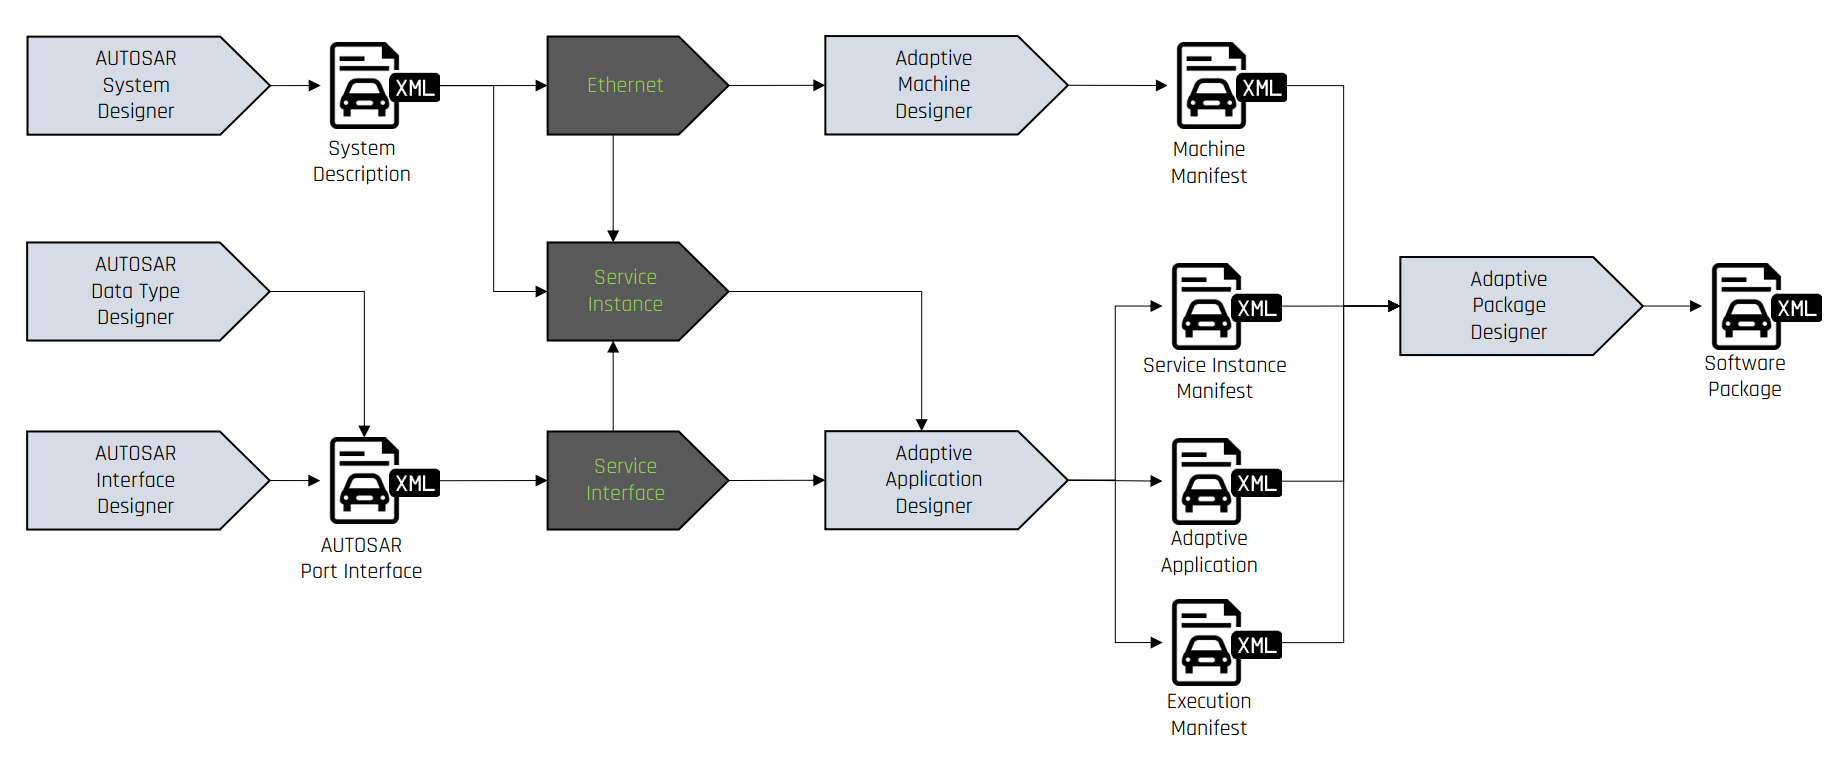
\includegraphics[width=1\textwidth]{Images/chapter2/aio_ap.png}
    \vspace{0.5cm}
    \caption{Adaptive Platform Workflow in AutoSAR.io \cite{popcornsar_intro}}
    \label{fig:autosar_io_ap}
\end{figure}


\begin{figure}[h]
    \centering
    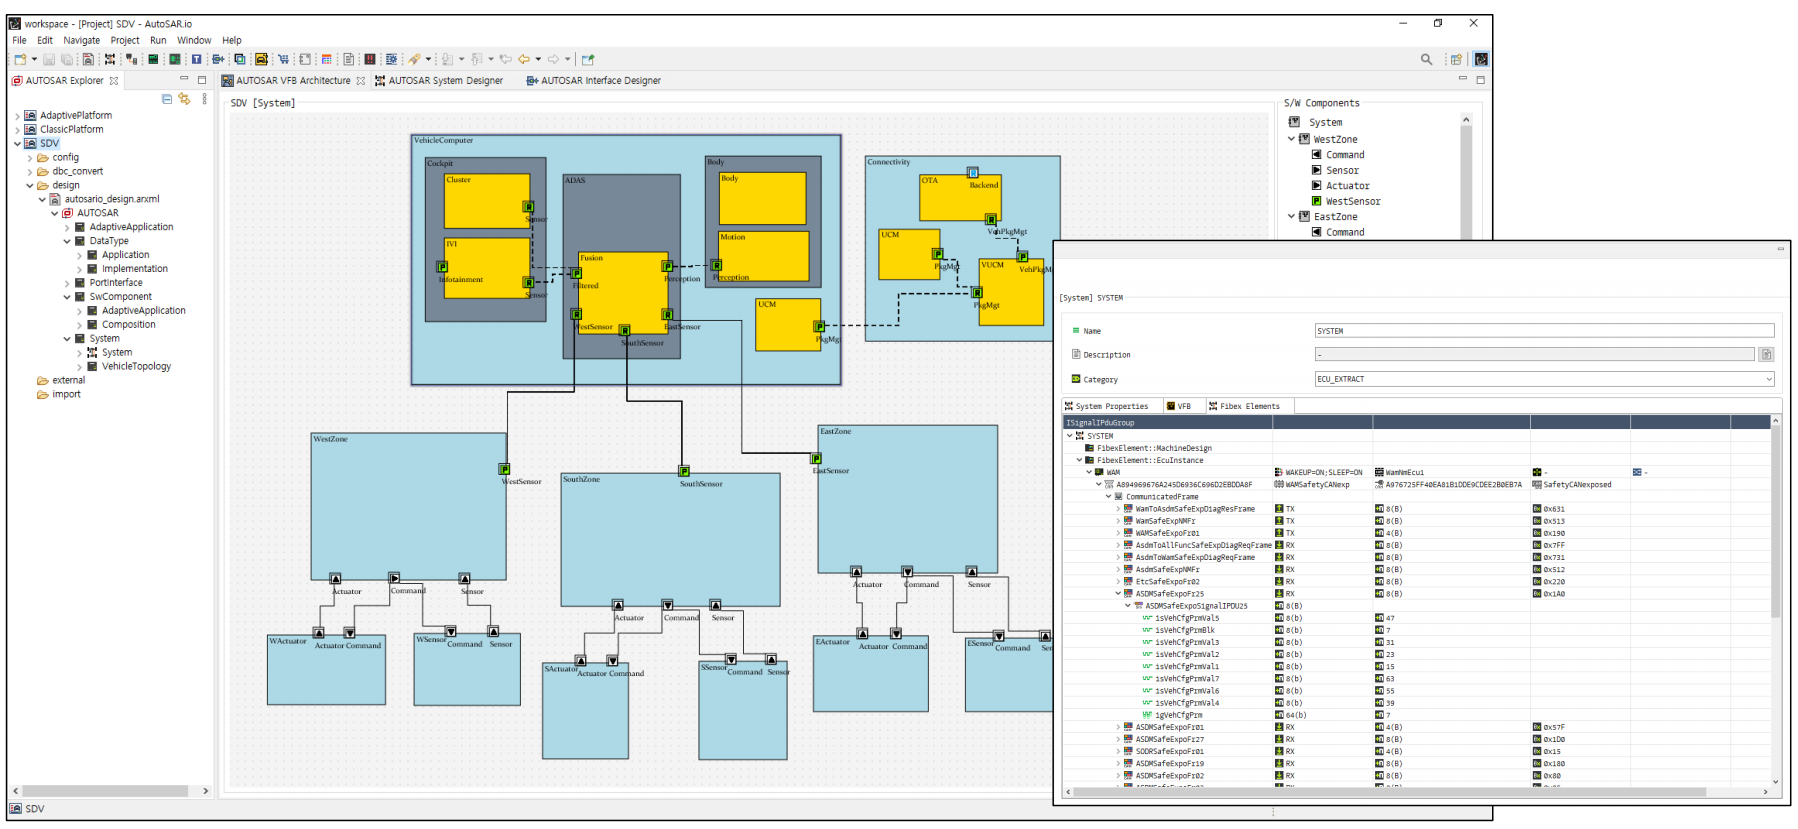
\includegraphics[width=1\textwidth]{Images/chapter2/aio_systemdesign.png}
    \vspace{0.5cm}
    \caption{AUTOSAR System Design in AutoSAR.io \cite{popcornsar_intro}}
    \label{fig:autosar_io_systemdesign}
\end{figure}

\begin{figure}[h]
    \centering
    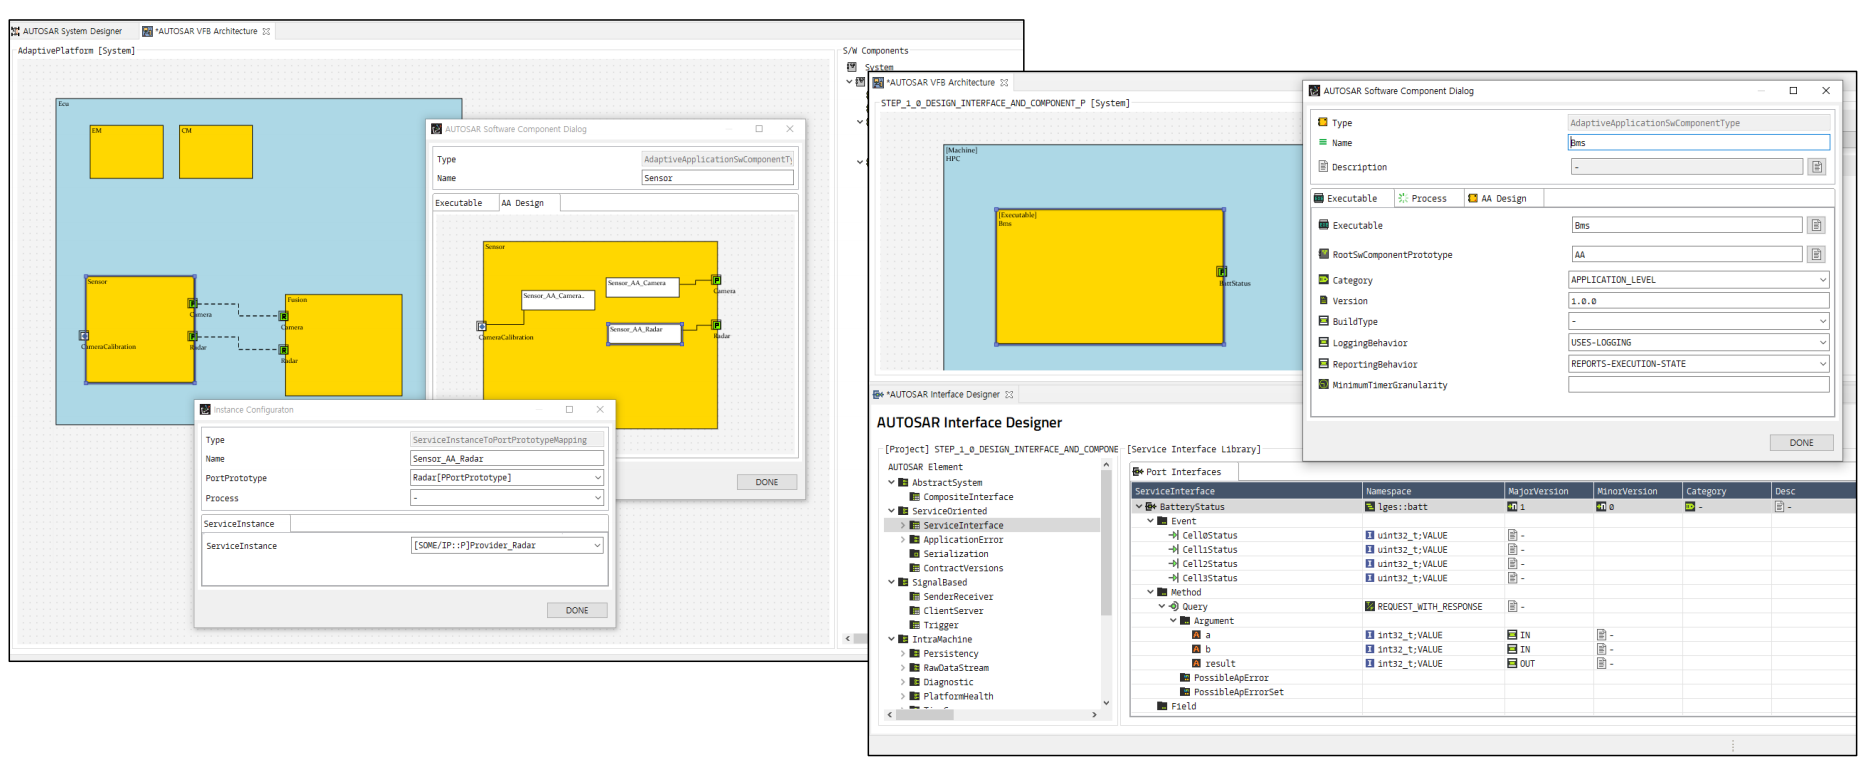
\includegraphics[width=1\textwidth]{Images/chapter2/aio_appldesign.png}
    \vspace{0.5cm}
    \caption{Application Design in AutoSAR.io \cite{popcornsar_intro}}
    \label{fig:autosar_io_appldesign}
\end{figure}


% \begin{figure}[h]
%     \centering
%     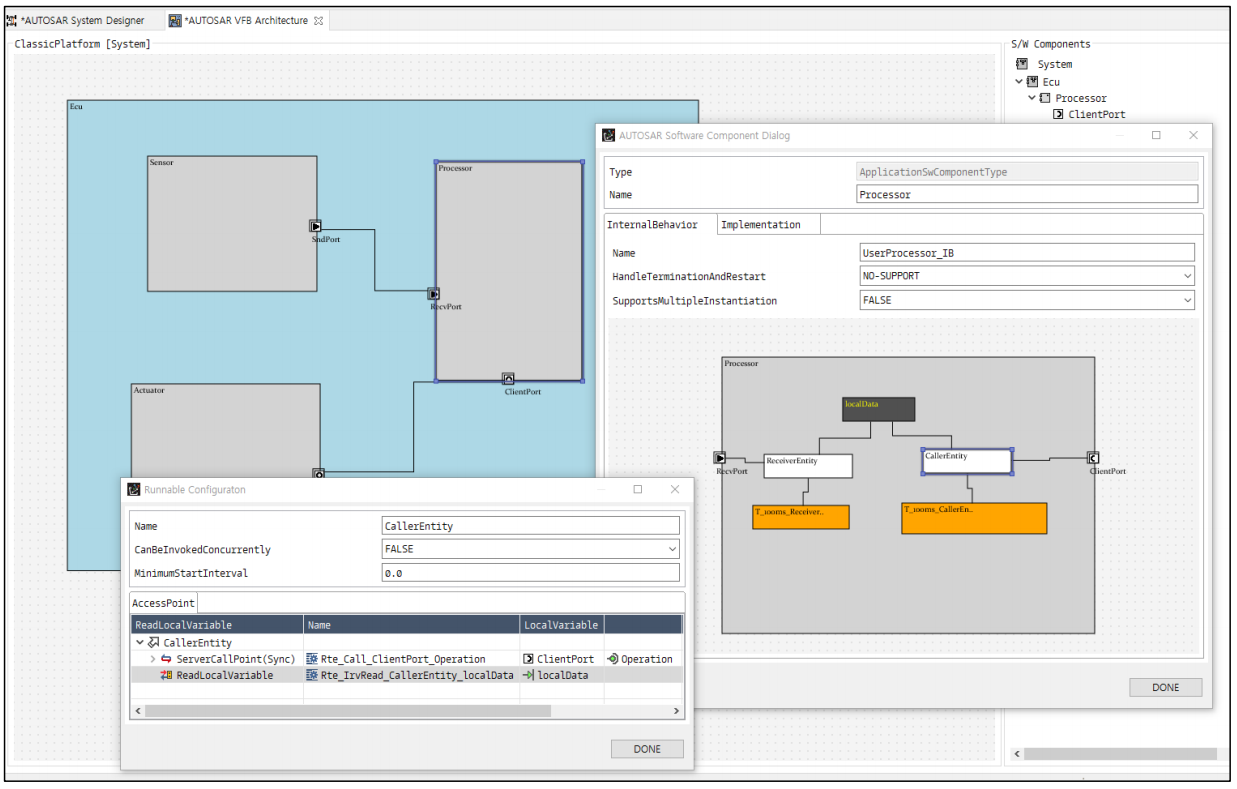
\includegraphics[width=1\textwidth]{Images/chapter2/aio_swdesign.png}
%     \vspace{0.5cm}
%     \caption{Software Component Design in AutoSAR.io \cite{popcornsar_intro}}
%     \label{fig:autosar_io_swdesign}
% \end{figure}

% \begin{figure}[h]
%     \centering
%     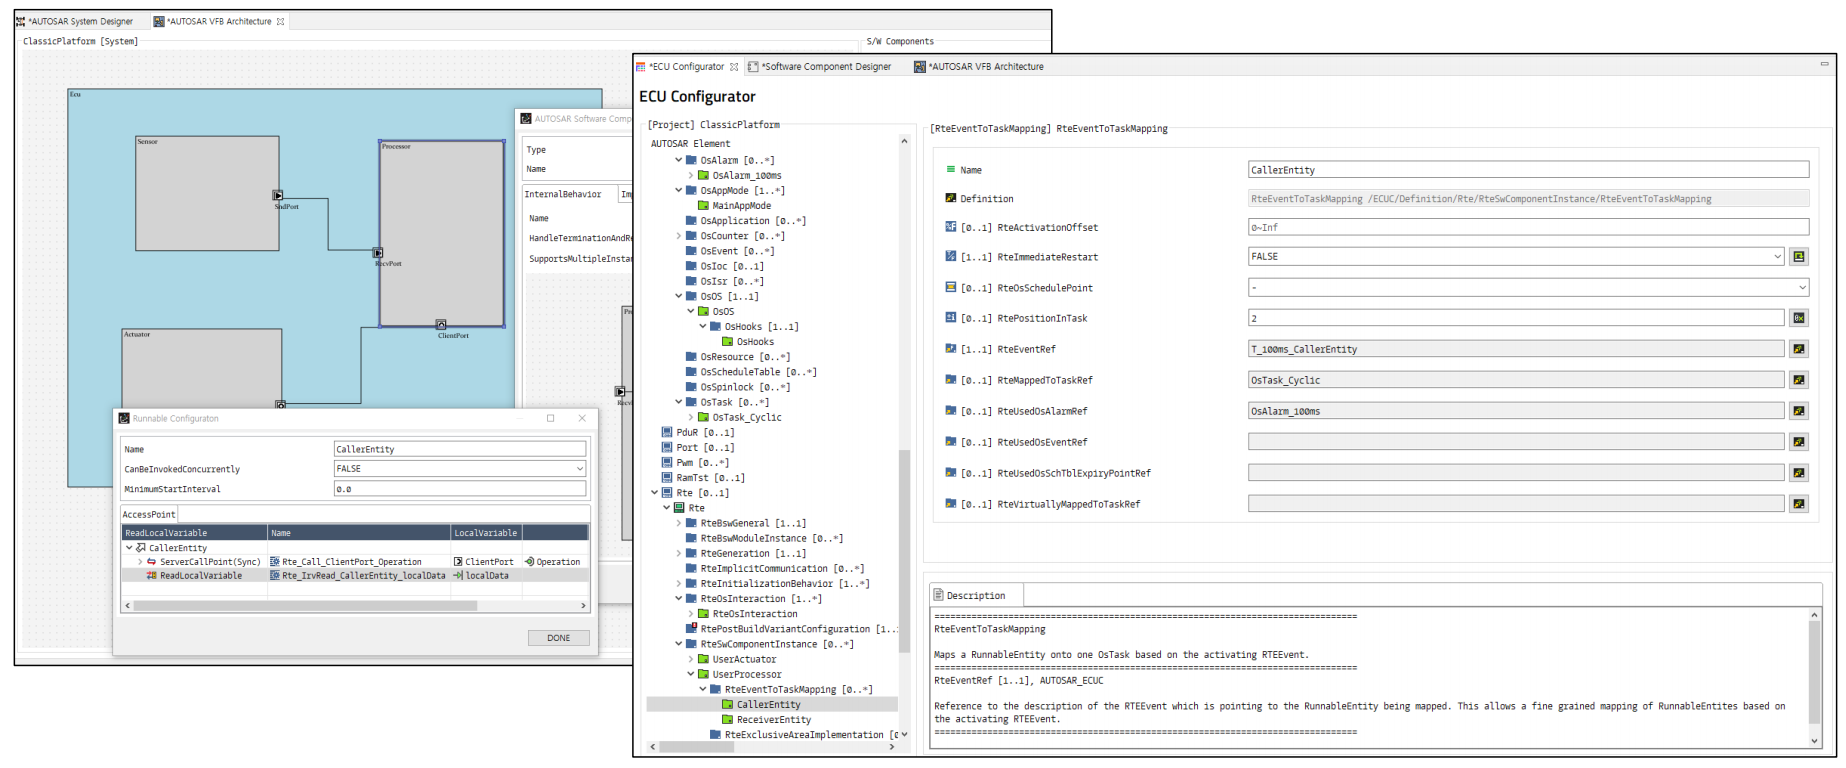
\includegraphics[width=1\textwidth]{Images/chapter2/aio_ecucfg.png}
%     \vspace{0.5cm}
%     \caption{ECU Configuration in AutoSAR.io \cite{popcornsar_intro}}
%     \label{fig:autosar_io_ecucfg}
% \end{figure}

AutoSAR.io is a powerful modeling tool that supports Code Generator of AUTOSAR-compliant code and manifest files. It streamlines development workflows while enabling full customization based on customer-specific requirements.

\begin{figure}[h]
    \centering
    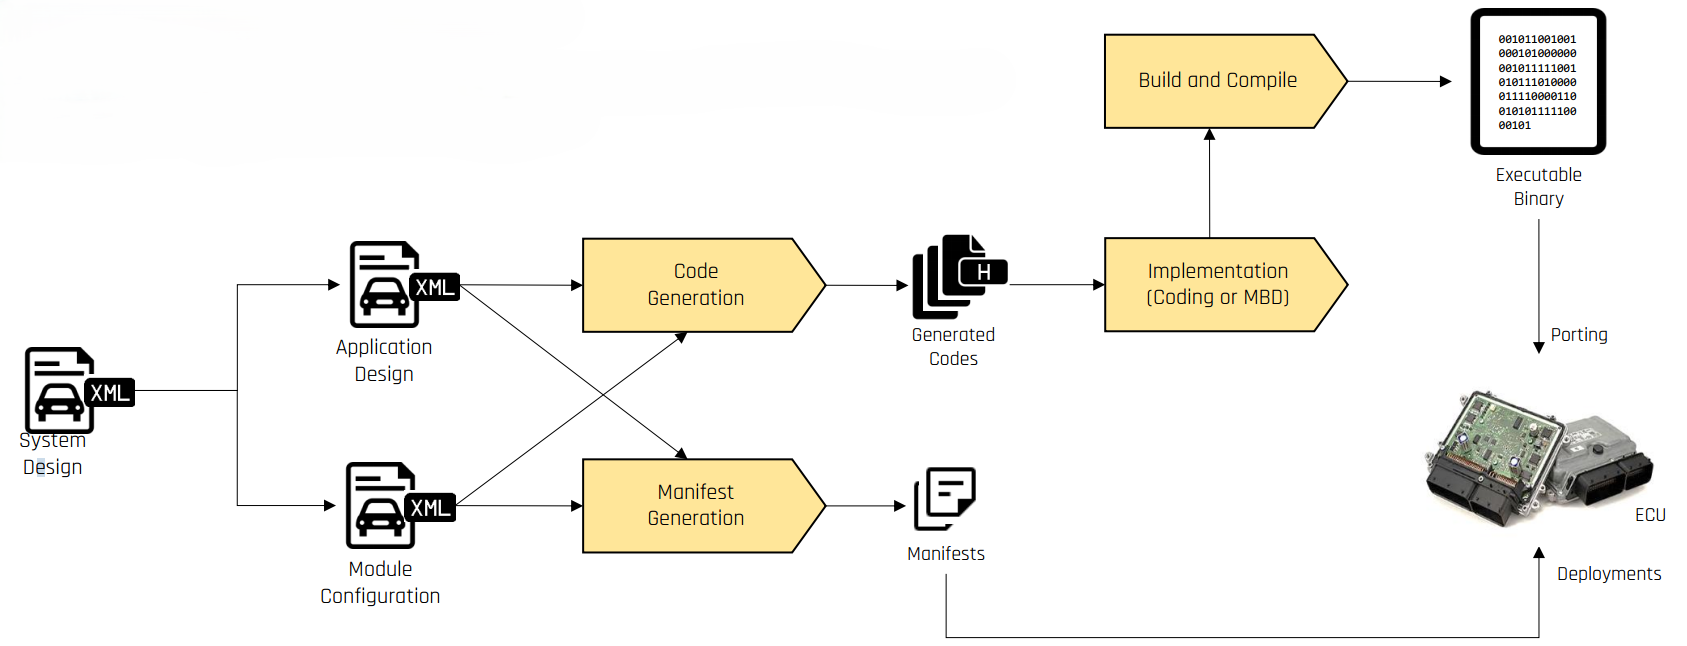
\includegraphics[width=1\textwidth]{Images/chapter2/aio_gen.png}
    \vspace{0.5cm}
    \caption{Code Generator Workflow in AutoSAR.io \cite{popcornsar_intro}}
    \label{fig:autosar_io_codegen}
\end{figure}

% AutoSAR.io supports seamless conversion of various data model formats such as CAN DBC, COVESA VSS, and AUTOSAR ARXML into AUTOSAR-compliant models. This allows smooth integration of existing vehicle data assets into the AUTOSAR eco-system.

% \begin{figure}[h]
%     \centering
%     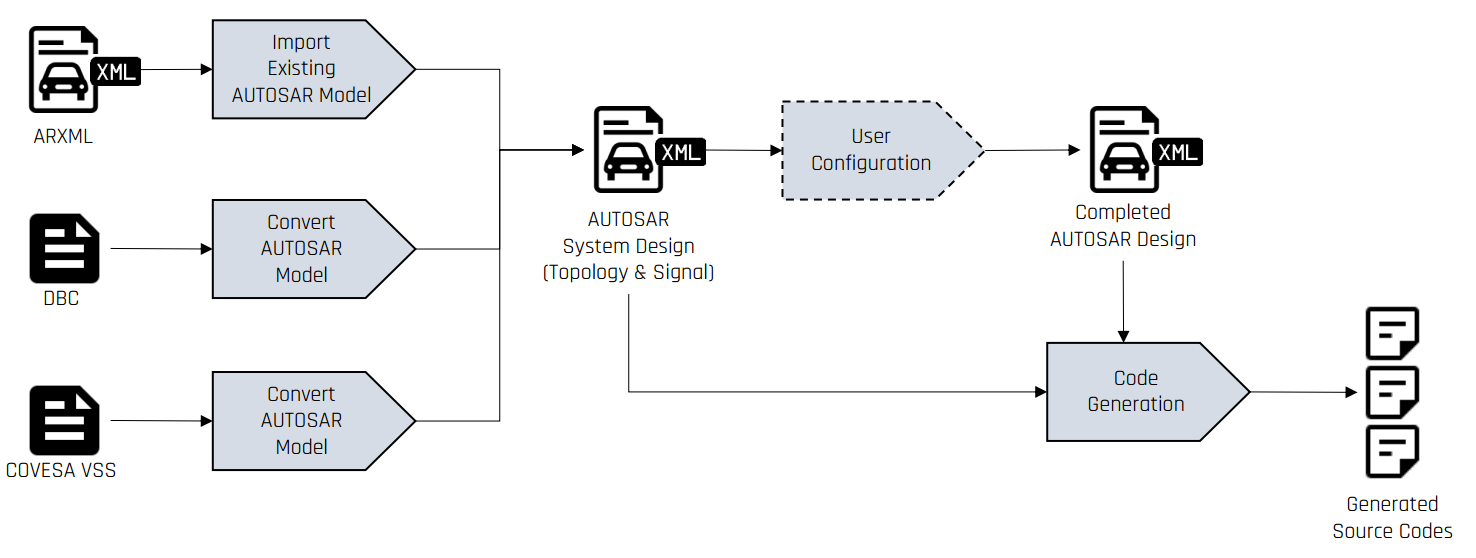
\includegraphics[width=1\textwidth]{Images/chapter2/aio_othergen.png}
%     \vspace{0.5cm}
%     \caption{Other Data Format Conversion Workflow in AutoSAR.io \cite{popcornsar_intro}}
%     \label{fig:autosar_io_othergen}
% \end{figure}
\newpage
\subsection{PARA}

PARA is PopcornSAR's ASIL-B certified AUTOSAR Adaptive Platform software framework, explicitly engineered for automotive HPC to accelerate the development of SDV. It delivers a comprehensive SOA that seamlessly integrates traditional automotive functions with modern IT frameworks like ROS2 and AI. To ensure robust operation across critical ADAS and VCU applications, PARA provides a suite of specialized functional clusters: \texttt{ara::com} manages diverse communication protocols (SOME/IP, DDS, zero-copy IPC, and Signal-To-Service), \texttt{ara::exec} orchestrates safe application lifecycles, and \texttt{ara::phm} enforces ISO 26262-compliant health monitoring. Furthermore, the SDK incorporates rigorous security mechanisms (\texttt{ara::idsm}, \texttt{ara::crypto}), diagnostic capabilities (\texttt{ara::diag}), secure Over-The-Air updates (\texttt{ara::ucm}), and legacy signal-based bridging (\texttt{para::sigcom}, \texttt{ara::aag}) to form a highly scalable, secure, and future-proof automotive development ecosystem.


\begin{figure}[h]
    \centering
    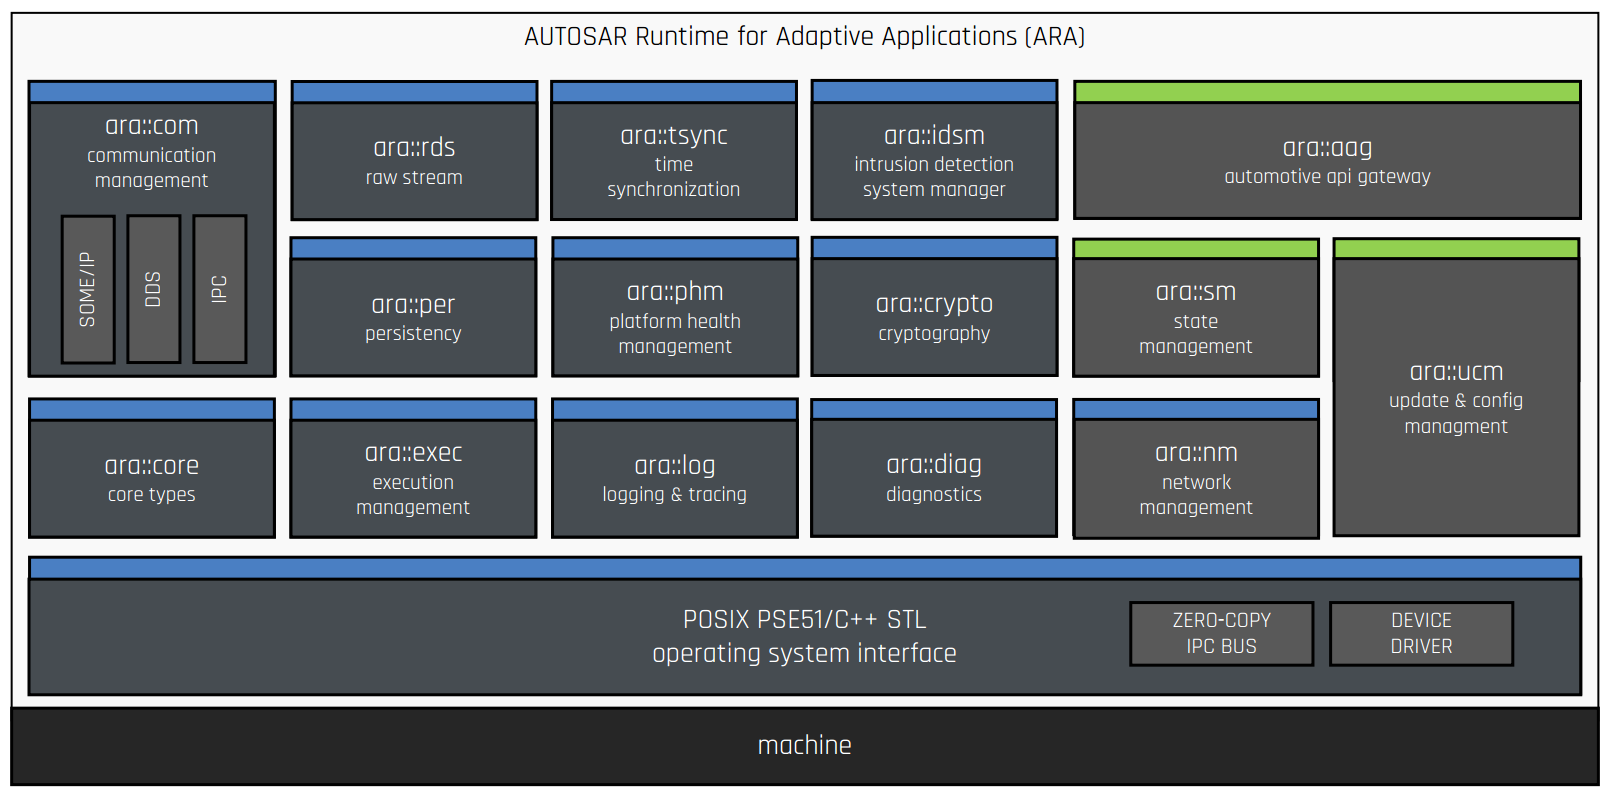
\includegraphics[width=1\textwidth]{Images/chapter2/para_basemodule.png}
    \vspace{0.5cm}
    \caption{Base Modules in PARA \cite{popcornsar_intro}}
    \label{fig:para_basemodule}
\end{figure}
\newpage
\paragraph*{Communication}(\texttt{ara::com})

\begin{figure}[h]
    \centering
    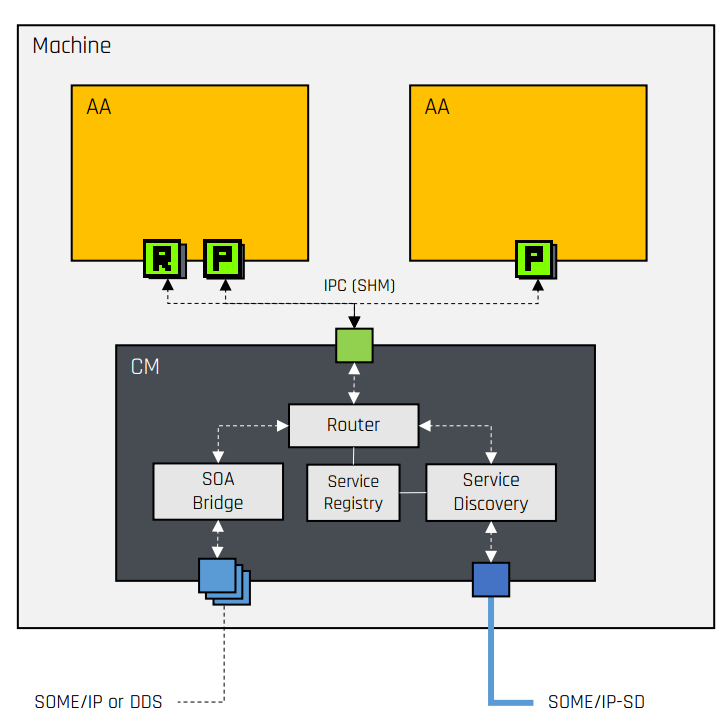
\includegraphics[width=0.5\textwidth]{Images/chapter2/para_com.png}
    \vspace{0.5cm}
    \caption{Communication in PARA \cite{popcornsar_intro}}
    \label{fig:para_com}
\end{figure}

PARA provides the complete product level for Service-Oriented Communication features. With PARA, \texttt{ara::com} provides full API and management for implementing service instances with application.

Some Protocols for SOA are supported in PARA like SOME/IP, DDS, and IPC (For Intra-machine).

PARA has base scheme for High-Performance IPC with zero-copy. 


\paragraph*{Execution Management}(\texttt{ara::exec})


\begin{figure}[h]
    \centering
    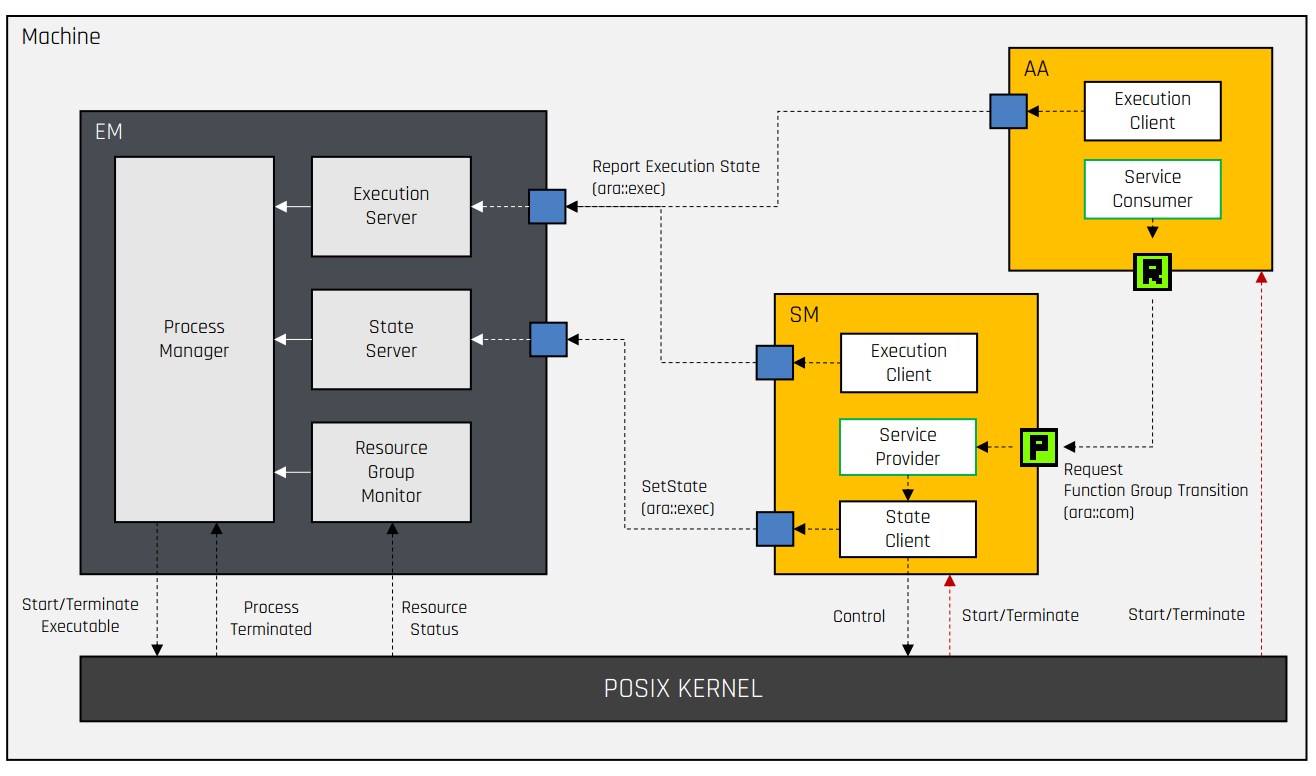
\includegraphics[width=0.8\textwidth]{Images/chapter2/para_exec.png}
    \vspace{0.5cm}
    \caption{Execution Management in PARA \cite{popcornsar_intro}}
    \label{fig:para_exec}
\end{figure}

With PARA, ara::exec provides management of applications with your configured scenario with state, execution dependency and resource statues. It also supports safe starting and termination of applications and machine.

After introducing the toolchain used to configure and generate Adaptive AUTOSAR applications, the following sections describe the AI models and inference runtime that provide the perception capability of the prototype.
% \newpage

% \section{YOLO (You Only Live Once) Model and MobileNetV4}



% \subsection{Overview of YOLO}

% The landscape of computer vision, particularly within the high-stakes domain of autonomous driving and Advanced Driver Assistance Systems (ADAS), has been irrevocably altered by the advent and evolution of the \textbf{``You Only Look Once"} (\textbf{YOLO}) architecture. As vehicles move towards higher levels of autonomy, the requirement for perception systems shifts from merely accurate classification to a rigorous demand for low-latency, high-frequency spatial understanding. Traffic light detection represents a particularly unforgiving subset of this domain: the targets are small, state-variant, and environmentally volatile, yet the system’s failure tolerance is effectively zero. This section explores the theoretical underpinnings of YOLO, tracing its dominance over two-stage detectors, and analyzes its suitability for the specific constraints of real-time traffic signal recognition.

% \subsubsection{The Single-Stage Revolution}

% Prior to the introduction of YOLO in 2015, the state-of-the-art in object detection was dominated by Region-based Convolutional Neural Networks (R-CNN) and its successors. These architectures operated on a "propose-and-verify" paradigm where a dedicated mechanism would hypothesize thousands of potential object locations before a classifier verified them. While this method achieved high average precision, it suffered from a fundamental decoupling of localization and classification, creating a computational bottleneck that rendered real-time performance on embedded hardware nearly impossible. YOLO proposed a radical unification by reframing object detection not as a classification task applied to generated regions, but as a single regression problem. In this paradigm, a single neural network processes the full image in one forward pass, predicting bounding box coordinates and class probabilities directly from the feature maps.

% This "single-shot" approach yields decisive advantages for traffic light detection. First, it enables global contextual reasoning. Unlike sliding window or region proposal approaches that see only a subset of the image pixels at any given time, the YOLO architecture views the entire image during both training and inference. This allows the network to implicitly encode contextual information about object classes, such as inferring the likelihood of a traffic light based on the presence of a pole or the geometry of an intersection, thereby significantly reducing background false positives. Second, YOLO offers inference latency stability. The processing time of a YOLO network is effectively constant for a given input resolution, regardless of the number of objects in the scene. For safety-critical control loops in autonomous vehicles, this deterministic latency is non-negotiable, ensuring the perception system delivers state estimates at a fixed cadence to the planning module.

% \subsubsection{Choosing YOLO26 for Real-Time Detection}
% The decision to utilize YOLO11 (released late 2024) for traffic light detection is driven by its specific architectural refinements designed for efficiency and small-object detection. YOLO11 represents a significant evolution over predecessors like v5 and v8, introducing enhanced feature aggregation through C3k2 blocks and C2PSA attention modules. These components significantly improve the extraction of fine-grained features necessary for resolving distant traffic lights. Furthermore, the YOLOv11n (Nano) variant achieves higher Mean Average Precision (mAP) than previous nano models with approximately 22\% fewer parameters. This parameter efficiency is critical for the constrained compute environments of embedded vehicular Electronic Control Units (ECUs), allowing for sophisticated detection logic without exceeding thermal or power budgets.


% \subsection{The YOLO Algorithmic Architecture}
% In this proposed system, while the MobileNetV4 backbone handles the heavy lifting of feature extraction, the detection logic relies on the advanced YOLOv11 Neck and Head. This architecture departs from previous iterations by introducing specific modules that optimize the feature fusion process and employs an anchor-free, decoupled head paradigm.

% \subsubsection{The Grid System and Feature Fusion (C3k2)}

% The core of YOLOv11's spatial reasoning remains its hierarchical grid system, derived from a Path Aggregation Network (PANet). The input image is not processed as a monolith but is partitioned into grids of varying granularity. The input image $I$ is processed into feature maps at three distinct scales: P3 (stride 8), P4 (stride 16), and P5 (stride 32). The Neck is responsible for fusing these maps to combine the semantic richness of deep layers with the spatial precision of shallow layers.

% A primary innovation in the YOLOv11 Neck is the use of the C3k2 (Cross Stage Partial with Kernel Size 2) block, which replaces the C2f block found in YOLOv8. The C3k2 block utilizes optimized kernel sizes and a streamlined gradient path, allowing for customizable kernel configurations. This design enables the model to extract features with faster processing speeds on hardware accelerators. For traffic light detection, this efficient fusion is critical when processing high-resolution images, such as $1280 \times 1280$ pixels, which are often required to resolve small signal lights. The C3k2 block prevents the feature fusion stage from becoming a latency bottleneck, ensuring the semantic context of the intersection is merged with the fine spatial detail of the signal head without incurring excessive computational cost.

% \subsubsection{C2PSA: Spatial Attention for Small Objects}

% A defining feature of YOLOv11 logic is the inclusion of the C2PSA (Cross Stage Partial with Spatial Attention) module, typically positioned at the end of the feature extraction phase. The C2PSA module introduces a parallel branch that computes a spatial attention map, forcing the network to weight specific pixels more heavily before passing features to the detection head. In the context of traffic lights, which often occupy less than 1\% of the total image area, background noise from the sky, buildings, or trees can dominate the feature map. The C2PSA mechanism effectively suppresses this background noise and amplifies the activation of the relevant signal pixels. This targeted attention significantly improves the recall for distant lights, ensuring that the network focuses its capacity on the objects of interest rather than the surrounding clutter.

% \subsubsection{Anchor-Free Bounding Box Regression}

% YOLOv11 employs a fully anchor-free detection head, a departure from older versions that relied on pre-defined anchor boxes. Instead of predicting offsets from prototypical shapes, YOLOv11 predicts the bounding box geometry directly from the center of the grid cell. For a grid cell at location $(c_x, c_y)$ that is deemed responsible for an object, the network regresses four values representing the distances to the box edges: Left ($l$), Top ($t$), Right ($r$), and Bottom ($b$). The predicted bounding box $\hat{B}$ is formulated as:

% \begin{equation}
%     \hat{B} = [c_x - l, c_y - t, c_x + r, c_y + b]
% \end{equation}

% This approach eliminates the need to tune anchor hyperparameters for specific datasets, making the model naturally adaptive to the varying aspect ratios of traffic signals, whether they are vertical stacks, horizontal arrays, or single-aspect beacons.

% \subsubsection{The Loss Function: Task Alignment and CIoU}

% The training of the YOLOv11 head is guided by a composite loss function that enforces strict alignment between the classification and localization tasks. Traditional detectors often predict a high class score even if the bounding box is inaccurate. To counter this, YOLOv11 utilizes Task Aligned Loss (TAL). TAL dynamically assigns labels based on the quality of the prediction, calculating an alignment metric $t$ as $t = s^\alpha \times u^\beta$, where $s$ is the predicted classification score and $u$ is the Intersection over Union (IoU) between the predicted box and the ground truth. This ensures that high confidence scores are only assigned to predictions that are both semantically correct and spatially precise.

% For localization, the system employs Complete IoU (CIoU) loss combined with Distribution Focal Loss (DFL). The CIoU loss minimizes geometric errors by considering overlap area, center point distance, and aspect ratio consistency. The formula is given by:

% \begin{equation}
%     \mathcal{L}_{CIoU} = 1 - IoU + \frac{\rho^2(b, b^{gt})}{c^2} + \alpha v
% \end{equation}


% Here, $\rho$ is the Euclidean distance between box centers, $c$ is the diagonal length of the smallest enclosing box, and $\alpha v$ measures the consistency of the aspect ratio. This forces the model to rapidly converge to the vertical rectangular shape typical of traffic lights. Furthermore, DFL handles the ambiguity of small, blurred traffic lights by modeling the box edges not as single deterministic numbers but as probability distributions. By optimizing the network to focus the probability density around the true edge location, DFL provides refined, sub-pixel accuracy that is vital for distant signals.

% \subsubsection{Post-Processing: Class-Agnostic NMS}

% Because the anchor-free head is dense, a single traffic light will often trigger detections in multiple adjacent grid cells. Non-Maximum Suppression (NMS) is the algorithm used to filter these duplicate candidates. For traffic light detection, Class-Agnostic NMS is strongly recommended. This logic prevents the physically impossible scenario of detecting both a "Green Light" and a "Red Light" in the exact same spatial location. By suppressing overlapping boxes regardless of their class label, the model is forced to commit to the single highest-confidence state, thereby reducing conflicting outputs for the downstream planning system.

% \subsection{MobileNetV4 Backbone Architecture}
% To maximize efficiency on edge hardware such as the Raspberry Pi or NVIDIA Jetson, this report proposes replacing the standard YOLO backbone with MobileNetV4 (MNv4). MNv4, introduced in 2024, represents the culmination of research into efficient neural network design, prioritizing "Universal Efficiency" to ensure operations run fast across CPUs, GPUs, and DSPs without the fragmentation seen in previous versions.
% \subsubsection{Evolution of MobileNets: From V1 to V4}

% The MobileNet lineage began with \textbf{MobileNetV1}, which introduced Depthwise Separable Convolutions to factorize standard convolution into spatial and channel steps, reducing computation by approximately nine times. \textbf{MobileNetV2} subsequently introduced the Inverted Residual Block and Linear Bottlenecks to preserve information flow in low-dimensional spaces. \textbf{MobileNetV3} later incorporated Neural Architecture Search (NAS) and Squeeze-and-Excitation (SE) blocks. However, V3's heterogeneous blocks and complex activation functions often resulted in poor performance on DSPs due to synchronization overhead. \textbf{MobileNetV4} addresses these issues by using unified blocks optimized for the hardware "Roofline Model", ensuring that the architecture stays at the optimal ridge point of operational intensity where every cycle of memory transfer is matched by maximum computation.

% \subsubsection{Universal Inverted Bottleneck (UIB)}

% The core innovation of MobileNetV4 is the Universal Inverted Bottleneck (UIB). This is a flexible search block that unifies previous architectures by introducing two optional depthwise convolutions that can be enabled or disabled via NAS. The UIB can instantiate as a standard Inverted Bottleneck for capacity, a ConvNext block for cheaper spatial mixing, or a novel ExtraDW block. The ExtraDW variant is particularly beneficial for traffic light detection. By adding extra depthwise layers at a low computational cost, it significantly increases the network's receptive field. This allows the backbone to "see" the entire intersection context—such as the traffic pole arm or the road geometry—without the heavy computational penalty of large kernels, which is crucial for identifying signal heads amidst urban clutter.

% \subsubsection{Mobile Multi-Query Attention (MQA)}

% Standard Multi-Head Self-Attention (MHSA) is typically memory-bound on mobile chips, making it slow to execute. To overcome this, MNv4 introduces Mobile MQA (Multi-Query Attention). In this mechanism, all query heads share a single Key and Value head, and a spatial reduction is applied via a stride-2 depthwise convolution. The attention computation can be approximated as:

% \begin{equation}
%     \text{Attention}(Q, K, V) = \text{Softmax}\left(\frac{Q \cdot (SR(K))^T}{\sqrt{d_k}}\right) \cdot SR(V)
% \end{equation}

% This design provides a substantial speedup—approximately 39\% on EdgeTPUs—while retaining the global context capabilities of transformers. This global attention helps the model distinguish true traffic lights from reflections or neon signs by analyzing the broader scene context, a capability that pure CNNs often lack.

% \subsubsection{Integrating MobileNetv4 into YOLO}

% Integrating MobileNetV4 as the feature extractor for YOLOv11 creates a hybrid "YOLO-MNv4" architecture that is theoretically optimal for autonomous driving. On mobile accelerators like the Pixel EdgeTPU, MNv4 is approximately twice as fast as MobileNetV3 for equivalent accuracy due to its high operational intensity. Replacing the standard YOLOv11 backbone with MNv4 significantly reduces the floating-point operations (FLOPs) required per inference. This architecture specifically excels in occlusion handling, where the advanced receptive fields of the UIB blocks allow the model to infer the presence of a traffic light even when it is partially obscured by large vehicles, ensuring a robust and reliable perception system.
\section{YOLO (You Only Look Once) Model and MobileNetV4 Backbone}



\subsection{Overview of YOLO}

The landscape of computer vision, particularly within the high-stakes domain of autonomous driving and Advanced Driver Assistance Systems (ADAS), has been irrevocably altered by the advent and evolution of the {``You Only Look Once"} ({YOLO}) architecture. As vehicles move towards higher levels of autonomy, the requirement for perception systems shifts from merely accurate classification to a rigorous demand for low-latency, high-frequency spatial understanding. Traffic light detection represents a particularly unforgiving subset of this domain: the targets are small, state-variant, and environmentally volatile, yet the system’s failure tolerance is effectively zero. This section explores the theoretical underpinnings of YOLO, tracing its dominance over two-stage detectors, and analyzes its suitability for the specific constraints of real-time traffic signal recognition.

\subsubsection{The Single-Stage Revolution}

Prior to the introduction of YOLO in 2015, the state-of-the-art in object detection was dominated by Region-based Convolutional Neural Networks (R-CNN) and its successors. These architectures operated on a "propose-and-verify" paradigm where a dedicated mechanism would hypothesize thousands of potential object locations before a classifier verified them. While this method achieved high average precision, it suffered from a fundamental decoupling of localization and classification, creating a computational bottleneck that rendered real-time performance on embedded hardware nearly impossible. YOLO proposed a radical unification by reframing object detection not as a classification task applied to generated regions, but as a single regression problem. In this paradigm, a single neural network processes the full image in one forward pass, predicting bounding box coordinates and class probabilities directly from the feature maps.

This "single-shot" approach yields decisive advantages for traffic light detection. First, it enables global contextual reasoning. Unlike sliding window or region proposal approaches that see only a subset of the image pixels at any given time, the YOLO architecture views the entire image during both training and inference. This allows the network to implicitly encode contextual information about object classes, such as inferring the likelihood of a traffic light based on the presence of a pole or the geometry of an intersection, thereby significantly reducing background false positives. Second, YOLO offers inference latency stability. The processing time of a YOLO network is effectively constant for a given input resolution, regardless of the number of objects in the scene. For safety-critical control loops in autonomous vehicles, this deterministic latency is non-negotiable, ensuring the perception system delivers state estimates at a fixed cadence to the planning module.

\subsubsection{YOLO26 for Real-Time Detection}
The decision to utilize YOLO26 (released January 2026) for traffic light detection is driven by its specific architectural refinements designed for efficiency and small-object detection. YOLO26 represents a significant evolution over predecessors like YOLO11 and YOLOv8 \cite{yolo26}, introducing enhanced feature aggregation through C3k2 blocks, C2PSA attention modules, and a novel MuSGD optimizer. These components significantly improve the extraction of fine-grained features necessary for resolving distant traffic lights. Furthermore, YOLO26 removes the Distribution Focal Loss (DFL) module entirely, simplifying export and hardware compatibility, and delivers up to 43\% faster CPU inference compared to its predecessors. This computational efficiency is critical for the constrained compute environments of embedded vehicular Electronic Control Units (ECUs), allowing for sophisticated detection logic without exceeding thermal or power budgets.


\subsection{The YOLO Algorithmic Architecture}
In this proposed system, while the MobileNetV4 backbone handles the heavy lifting of feature extraction, the detection logic relies on the advanced YOLO26 Neck and Head. This architecture departs from previous iterations by introducing specific modules that optimize the feature fusion process and employs an anchor-free, decoupled head paradigm.

\subsubsection{The Grid System and Feature Fusion (C3k2)}

The core of YOLO26's spatial reasoning remains its hierarchical grid system, derived from a Path Aggregation Network (PANet). The input image is not processed as a monolith but is partitioned into grids of varying granularity. In the standard YOLO26-p2 configuration, the backbone produces feature maps at four scales: P2 (stride 4), P3 (stride 8), P4 (stride 16), and P5 (stride 32). In the proposed system, the Neck fuses these maps to combine the semantic richness of deep layers with the spatial precision of shallow layers.

A primary innovation in the YOLO26 Neck is the use of the C3k2 (Cross Stage Partial with Kernel Size 2) block, inherited from YOLO11 and refined in YOLO26. The C3k2 block utilizes a cross-stage partial design with customizable kernel configurations and a streamlined gradient path. This design enables the model to extract features with faster processing speeds on hardware accelerators. For traffic light detection in this system, images are processed at $416 \times 416$ pixels—a resolution chosen to balance inference speed with the spatial detail required to resolve signal heads on edge hardware. The C3k2 block prevents the feature fusion stage from becoming a latency bottleneck, ensuring the semantic context of the intersection is merged with the fine spatial detail of the signal head without incurring excessive computational cost.

\subsubsection{C2PSA: Spatial Attention for Small Objects}

A defining feature of YOLO26 logic is the inclusion of the C2PSA (Cross Stage Partial with Spatial Attention) module, typically positioned at the end of the feature extraction phase. The C2PSA module introduces a parallel branch that computes a spatial attention map, forcing the network to weight specific pixels more heavily before passing features to the detection head. In the context of traffic lights, which often occupy less than 1\% of the total image area, background noise from the sky, buildings, or trees can dominate the feature map. The C2PSA mechanism effectively suppresses this background noise and amplifies the activation of the relevant signal pixels. This targeted attention significantly improves the recall for distant lights, ensuring that the network focuses its capacity on the objects of interest rather than the surrounding clutter.

% \subsubsection{Anchor-Free Bounding Box Regression}

% YOLO26 employs a fully anchor-free detection head, a departure from older versions that relied on pre-defined anchor boxes. Instead of predicting offsets from prototypical shapes, YOLO26 predicts the bounding box geometry directly from the center of the grid cell. For a grid cell at location $(c_x, c_y)$ that is deemed responsible for an object, the network regresses four values representing the distances to the box edges: Left ($l$), Top ($t$), Right ($r$), and Bottom ($b$). The predicted bounding box $\hat{B}$ is formulated as:

% \begin{equation}
%     \hat{B} = [c_x - l, c_y - t, c_x + r, c_y + b]
% \end{equation}

% This approach eliminates the need to tune anchor hyperparameters for specific datasets, making the model naturally adaptive to the varying aspect ratios of traffic signals, whether they are vertical stacks, horizontal arrays, or single-aspect beacons.

% \subsubsection{The Loss Function: Task Alignment and CIoU}

% The training of the YOLO26 head is guided by a composite loss function that enforces strict alignment between the classification and localization tasks. Traditional detectors often predict a high class score even if the bounding box is inaccurate. To counter this, YOLO26 utilizes a Spatial and Task-Aligned Label assignment (STAL), a component of ProgLoss. STAL dynamically assigns labels based on the quality of the prediction, calculating an alignment metric $t$ as $t = s^\alpha \times u^\beta$, where $s$ is the predicted classification score, $u$ is the Intersection over Union (IoU) between the predicted box and the ground truth, and $\alpha$, $\beta$ are balancing hyperparameters. This ensures that high confidence scores are only assigned to predictions that are both semantically correct and spatially precise.

% For localization, YOLO26 employs Complete IoU (CIoU) loss. A key distinction from its predecessors is that {YOLO26 removes Distribution Focal Loss (DFL) entirely}-this simplifies the model graph, broadens hardware compatibility, and reduces export complexity. The CIoU loss minimizes geometric errors by jointly considering overlap area, center-point distance, and aspect ratio consistency. The formula is given by:

% \begin{equation}
%     \mathcal{L}_{CIoU} = 1 - \text{IoU} + \frac{\rho^2(b, b^{gt})}{c^2} + \alpha v
% \end{equation}

% where $v = \frac{4}{\pi^2}\left(\arctan\frac{w^{gt}}{h^{gt}} - \arctan\frac{w}{h}\right)^2$ measures aspect ratio consistency, $\alpha = \frac{v}{(1-\text{IoU})+v}$ is a trade-off parameter, $\rho$ is the Euclidean distance between predicted box center $b$ and ground-truth center $b^{gt}$, and $c$ is the diagonal length of the smallest enclosing box. This formulation forces the model to converge to the vertical rectangular shape typical of traffic light signal heads.

\subsubsection{Dual-Head Architecture and NMS-Free Inference}

YOLO26 features a dual-head architecture that provides flexibility for different deployment scenarios \cite{yolo26}:
\begin{itemize}
    \item \textbf{One-to-One Head (Default)}: Produces end-to-end predictions without Non-Maximum Suppression (NMS), outputting $(N, 300, 6)$ with a maximum of 300 detections per image. This head is optimized for fast inference and simplified deployment.
    \item \textbf{One-to-Many Head}: Generates traditional YOLO outputs requiring NMS post-processing, outputting $(N, nc + 4, 8400)$ where $nc$ is the number of classes. This head typically achieves slightly higher accuracy at the cost of additional processing.
\end{itemize}

For the specific constraints of autonomous driving where deterministic latency is paramount, this proposed architecture chooses the free-NMS One-to-One Head (Default). By eliminating the NMS post-processing step entirely, the system avoids the variable computational overhead associated with filtering overlapping bounding boxes, thereby optimizing the end-to-end inference time on edge devices without compromising the determinism of the perception loop.

\subsection{MobileNetV4 Backbone Architecture}
To maximize efficiency on edge hardware such as the Raspberry Pi or NVIDIA Jetson, this report proposes replacing the standard YOLO backbone with MobileNetV4 (MNv4). MNv4, introduced in 2024, represents the culmination of research into efficient neural network design, prioritizing "Universal Efficiency" to ensure operations run fast across CPUs, GPUs, and DSPs without the fragmentation seen in previous versions.
\subsubsection{Evolution of MobileNets: From V1 to V4}

The MobileNet lineage began with {MobileNetV1}, which introduced Depthwise Separable Convolutions to factorize standard convolution into spatial and channel steps, reducing computation by approximately nine times. {MobileNetV2} subsequently introduced the Inverted Residual Block and Linear Bottlenecks to preserve information flow in low-dimensional spaces. {MobileNetV3} later incorporated Neural Architecture Search (NAS) and Squeeze-and-Excitation (SE) blocks. However, V3's heterogeneous blocks and complex activation functions often resulted in poor performance on DSPs due to synchronization overhead. {MobileNetV4} addresses these issues by using unified blocks optimized for the hardware "Roofline Model", ensuring that the architecture stays at the optimal ridge point of operational intensity where every cycle of memory transfer is matched by maximum computation.

\subsubsection{Universal Inverted Bottleneck (UIB)}

The core innovation of MobileNetV4 is the Universal Inverted Bottleneck (UIB). This is a flexible search block that unifies previous architectures by introducing two optional depthwise convolutions that can be enabled or disabled via NAS. The UIB can instantiate as a standard Inverted Bottleneck for capacity, a ConvNext block for cheaper spatial mixing, or a novel ExtraDW block. The ExtraDW variant is particularly beneficial for traffic light detection. By adding extra depthwise layers at a low computational cost, it significantly increases the network's receptive field. This allows the backbone to "see" the entire intersection context-such as the traffic pole arm or the road geometry-without the heavy computational penalty of large kernels, which is crucial for identifying signal heads amidst urban clutter.

\subsubsection{Mobile Multi-Query Attention (MQA)}

Standard Multi-Head Self-Attention (MHSA) is typically memory-bound on mobile chips, making it slow to execute. To overcome this, MNv4 introduces Mobile MQA (Multi-Query Attention). In this mechanism, all query heads share a single Key and Value projection, dramatically reducing memory bandwidth requirements. To further improve operational intensity, Spatial Reduction Attention (SRA) is incorporated: the key and value inputs are spatially downsampled using a stride-2 $3\times3$ depthwise convolution before projection, while the queries retain full resolution. The Mobile MQA block is formulated as (Eq. 2 in \cite{qin2024mobilenetv4universalmodels}):

\begin{equation}
    \text{attention}_j = \text{Softmax}\left(\frac{(X W^{Q_j}) \cdot (SR(X) W^K)^T}{\sqrt{d_k}}\right) \cdot SR(X) W^V
\end{equation}

where $SR$ denotes the stride-2 depthwise convolution for spatial reduction (or the identity function when spatial reduction is not applied), $W^{Q_j}$ is the query projection for head $j$, and $W^K$, $W^V$ are the shared key and value projections across all heads. This design provides a substantial speedup-over 39\% on EdgeTPUs-while retaining the global context capabilities of transformers. This global attention helps the model distinguish true traffic lights from reflections or neon signs by analyzing the broader scene context, a capability that pure CNNs often lack.

After establishing the model architecture, the next theoretical component is the inference runtime required to execute this model efficiently on the target edge device.

% \subsubsection{Integrating MobileNetv4 into YOLO}

% Integrating MobileNetV4 as the feature extractor for YOLO26 creates a hybrid "YOLO-MNv4" architecture that is theoretically optimal for autonomous driving. On mobile accelerators like the Pixel EdgeTPU, MNv4 is approximately twice as fast as MobileNetV3 for equivalent accuracy due to its high operational intensity. Replacing the standard YOLO26 backbone with MNv4 significantly reduces the floating-point operations (FLOPs) required per inference. This architecture specifically excels in occlusion handling, where the advanced receptive fields of the UIB blocks allow the model to infer the presence of a traffic light even when it is partially obscured by large vehicles, ensuring a robust and reliable perception system.


% To adapt the original YOLO26 architecture for edge deployment, several crucial modifications were made (comparing Figure \ref{fig:yolo26_original_arch} to Figure \ref{fig:yolo26_mnv4_arch}). First, the standard heavy CNN backbone was replaced entirely with {MobileNetV4ConvSmall050}. Second, the original 4-head Feature Pyramid Network (P2, P3, P4, P5) was scaled down to a {3-head architecture} (P3, P4, P5) by removing the high-resolution P2 feature extraction path and its corresponding detection head. This reduction dramatically lowers the computational complexity (GFLOPs) and parameter count. Meanwhile, the advanced components of the YOLO26 neck—including the {C3k2} fusion blocks, {SPPF}, {C2PSA} spatial attention, and the {One-to-One Head}-were preserved to maintain state-of-the-art detection logic.

% \begin{figure}[htbp]
%     \centering
%     \resizebox{\textwidth}{!}{
%     \begin{tikzpicture}[
%         box/.style={rectangle, draw, minimum width=2.4cm, minimum height=0.8cm, text centered, font=\sffamily, rounded corners=2pt},
%         arrow/.style={->, >=stealth, thick},
%         label/.style={font=\sffamily\scriptsize}
%     ]

%     % Backbone
%     \node[box, fill=blue!10] (input) at (0, 9) {Input (640)};
%     \node[box, fill=green!10] (conv1) at (0, 7.5) {Conv P1};
%     \node[box, fill=green!10] (p2) at (0, 6) {P2 (C3k2)};
%     \node[box, fill=green!10] (p3) at (0, 4) {P3 (C3k2)};
%     \node[box, fill=green!10] (p4) at (0, 2) {P4 (C3k2)};
%     \node[box, fill=green!10] (p5) at (0, 0) {P5 (C2PSA)};

%     \draw[arrow] (input) -- (conv1);
%     \draw[arrow] (conv1) -- (p2);
%     \draw[arrow] (p2) -- (p3);
%     \draw[arrow] (p3) -- (p4);
%     \draw[arrow] (p4) -- (p5);

%     % SPPF & C2PSA
%     \node[box, fill=yellow!10] (sppf) at (3.5, 0) {SPPF};
%     \node[box, fill=yellow!10] (c2psa) at (7.0, 0) {C2PSA};
%     \draw[arrow] (p5) -- (sppf);
%     \draw[arrow] (sppf) -- (c2psa);

%     % Neck - Top-down
%     \node[box, fill=orange!10] (cat_p4) at (7.0, 2) {Concat};
%     \node[box, fill=orange!10] (c3k2_td_p4) at (10.5, 2) {C3k2};
%     \draw[arrow] (c2psa) -- node[right, label] {Up} (cat_p4);
%     \draw[arrow] (p4) -- (cat_p4);
%     \draw[arrow] (cat_p4) -- (c3k2_td_p4);

%     \node[box, fill=orange!10] (cat_p3) at (10.5, 4) {Concat};
%     \node[box, fill=orange!10] (c3k2_td_p3) at (14.0, 4) {C3k2};
%     \draw[arrow] (c3k2_td_p4) -- node[right, label] {Up} (cat_p3);
%     \draw[arrow] (p3) -- (cat_p3);
%     \draw[arrow] (cat_p3) -- (c3k2_td_p3);

%     \node[box, fill=orange!10] (cat_p2) at (14.0, 6) {Concat};
%     \node[box, fill=orange!10] (c3k2_td_p2) at (17.5, 6) {C3k2};
%     \draw[arrow] (c3k2_td_p3) -- node[right, label] {Up} (cat_p2);
%     \draw[arrow] (p2) -- (cat_p2);
%     \draw[arrow] (cat_p2) -- (c3k2_td_p2);

%     % Neck - Bottom-up
%     \node[box, fill=orange!10] (cat_p3_bu) at (17.5, 4) {Concat};
%     \node[box, fill=orange!10] (c3k2_bu_p3) at (21.0, 4) {C3k2};
%     \draw[arrow] (c3k2_td_p2) -- node[right, label] {Conv s2} (cat_p3_bu);
%     \draw[arrow] (c3k2_td_p3) -- (cat_p3_bu);
%     \draw[arrow] (cat_p3_bu) -- (c3k2_bu_p3);

%     \node[box, fill=orange!10] (cat_p4_bu) at (21.0, 2) {Concat};
%     \node[box, fill=orange!10] (c3k2_bu_p4) at (24.5, 2) {C3k2};
%     \draw[arrow] (c3k2_bu_p3) -- node[right, label] {Conv s2} (cat_p4_bu);
%     \draw[arrow] (c3k2_td_p4) -- (cat_p4_bu);
%     \draw[arrow] (cat_p4_bu) -- (c3k2_bu_p4);

%     \node[box, fill=orange!10] (cat_p5_bu) at (24.5, 0) {Concat};
%     \node[box, fill=orange!10] (c3k2_bu_p5) at (28.0, 0) {C3k2};
%     \draw[arrow] (c3k2_bu_p4) -- node[right, label] {Conv s2} (cat_p5_bu);
%     \draw[arrow] (c2psa) -- (cat_p5_bu);
%     \draw[arrow] (cat_p5_bu) -- (c3k2_bu_p5);

%     % Detectors
%     \node[box, fill=red!10] (head2) at (31.5, 6) {Detect P2};
%     \node[box, fill=red!10] (head3) at (31.5, 4) {Detect P3};
%     \node[box, fill=red!10] (head4) at (31.5, 2) {Detect P4};
%     \node[box, fill=red!10] (head5) at (31.5, 0) {Detect P5};
    
%     \node[box, fill=purple!10, align=center, minimum height=1.6cm] (detect) at (35.0, 3) {One-to-One\\Head};

%     \draw[arrow] (c3k2_td_p2) -- (head2);
%     \draw[arrow] (c3k2_bu_p3) -- (head3);
%     \draw[arrow] (c3k2_bu_p4) -- (head4);
%     \draw[arrow] (c3k2_bu_p5) -- (head5);
    
%     \draw[arrow] (head2) -| (detect);
%     \draw[arrow] (head3) -| (detect);
%     \draw[arrow] (head4) -| (detect);
%     \draw[arrow] (head5) -| (detect);

%     \end{tikzpicture}
%     }
%     \vspace{0.5cm}
%     \caption{Architecture of the original YOLO26-p2 model with 4-head detection mechanism (P2/P3/P4/P5 outputs) for standard object detection tasks. Channel widths scale with the chosen model variant (n/s/m/l/x).}
%     \label{fig:yolo26_original_arch}
% \end{figure}





% \begin{figure}[htbp]
%     \centering
%     \resizebox{\textwidth}{!}{
%     \begin{tikzpicture}[
%         box/.style={rectangle, draw, minimum width=2.4cm, minimum height=0.8cm, text centered, font=\sffamily, rounded corners=2pt},
%         arrow/.style={->, >=stealth, thick},
%         label/.style={font=\sffamily\scriptsize}
%     ]

%     % X coordinates:
%     % 0.0: Backbone
%     % 3.5: SPPF
%     % 7.0: C2PSA, cat1
%     % 10.5: c3k2_1, cat2
%     % 14.0: c3k2_2, cat3
%     % 17.5: c3k2_3, cat4
%     % 21.0: c3k2_4
%     % 24.5: Detectors
%     % 28.0: Head

%     % Backbone
%     \node[box, fill=blue!10] (input) at (0, 8) {Input (416)};
%     \node[box, fill=green!10] (mnv4) at (0, 6) {MobileNetV4};
%     \node[box, fill=green!10] (p3) at (0, 4) {P3 (32c)};
%     \node[box, fill=green!10] (p4) at (0, 2) {P4 (48c)};
%     \node[box, fill=green!10] (p5) at (0, 0) {P5 (640c)};

%     \draw[arrow] (input) -- (mnv4);
%     \draw[arrow] (mnv4) -- (p3);
%     \draw[arrow] (p3) -- (p4);
%     \draw[arrow] (p4) -- (p5);

%     % SPPF & C2PSA
%     \node[box, fill=yellow!10] (sppf) at (3.5, 0) {SPPF (256c)};
%     \node[box, fill=yellow!10] (c2psa) at (7.0, 0) {C2PSA (256c)};
%     \draw[arrow] (p5) -- (sppf);
%     \draw[arrow] (sppf) -- (c2psa);

%     % Neck - Top-down
%     \node[box, fill=orange!10] (cat1) at (7.0, 2) {Concat};
%     \node[box, fill=orange!10] (c3k2_1) at (10.5, 2) {C3k2 (128c)};
%     \draw[arrow] (c2psa) -- node[right, label] {Up} (cat1);
%     \draw[arrow] (p4) -- (cat1);
%     \draw[arrow] (cat1) -- (c3k2_1);

%     \node[box, fill=orange!10] (cat2) at (10.5, 4) {Concat};
%     \node[box, fill=orange!10] (c3k2_2) at (14.0, 4) {C3k2 (64c)};
%     \draw[arrow] (c3k2_1) -- node[right, label] {Up} (cat2);
%     \draw[arrow] (p3) -- (cat2);
%     \draw[arrow] (cat2) -- (c3k2_2);

%     % Neck - Bottom-up
%     \node[box, fill=orange!10] (cat3) at (14.0, 2) {Concat};
%     \node[box, fill=orange!10] (c3k2_3) at (17.5, 2) {C3k2 (128c)};
%     \draw[arrow] (c3k2_2) -- node[right, label] {Conv s2} (cat3);
%     \draw[arrow] (c3k2_1) -- (cat3);
%     \draw[arrow] (cat3) -- (c3k2_3);

%     \node[box, fill=orange!10] (cat4) at (17.5, 0) {Concat};
%     \node[box, fill=orange!10] (c3k2_4) at (21.0, 0) {C3k2 (256c)};
%     \draw[arrow] (c3k2_3) -- node[right, label] {Conv s2} (cat4);
%     \draw[arrow] (c2psa) -- (cat4);
%     \draw[arrow] (cat4) -- (c3k2_4);

%     % Detectors
%     \node[box, fill=red!10] (head1) at (24.5, 4) {Detect P3};
%     \node[box, fill=red!10] (head2) at (24.5, 2) {Detect P4};
%     \node[box, fill=red!10] (head3) at (24.5, 0) {Detect P5};
    
%     \node[box, fill=purple!10, align=center] (detect) at (28.0, 2) {One-to-One\\Head};

%     \draw[arrow] (c3k2_2) -- (head1);
%     \draw[arrow] (c3k2_3) -- (head2);
%     \draw[arrow] (c3k2_4) -- (head3);
    
%     \draw[arrow] (head1) -| (detect);
%     \draw[arrow] (head2) -- (detect);
%     \draw[arrow] (head3) -| (detect);

%     \end{tikzpicture}
%     }
%     \vspace{0.5cm} % Add some space before caption to prevent overlap
%     \caption{Architecture of the YOLO26 model with MobileNetV4ConvSmall050 backbone, dual-head mechanism, and NMS-free end-to-end detection, tailored for $416\times416$ resolution.}
%     \label{fig:yolo26_mnv4_arch}
% \end{figure}


\section{Google LiteRT Framework}
\label{sec:litert}

LiteRT is Google's runtime for on-device AI inference, officially introduced in 2024 as the successor and rebrand of TensorFlow Lite (TFLite).  While TFLite had been the de-facto standard for deploying machine-learning models on mobile and embedded platforms since 2017, its tight coupling to the TensorFlow ecosystem and limited support for emerging model formats motivated Google to unify on-device inference under the LiteRT name.

\subsection{Relationship to TensorFlow Lite}

LiteRT retains full backward compatibility with the existing TFLite flatbuffer format (\texttt{.tflite}): any model previously exported for TFLite runs unmodified under LiteRT.  The core interpreter, delegate system, and quantisation toolchain remain unchanged, so the migration path from TFLite to LiteRT is a package rename with no model re-export required.  In Python, the import path changes from \texttt{tensorflow.lite} to the standalone \texttt{litert} package, decoupling the runtime from the full TensorFlow installation and reducing the deployment footprint on storage-constrained devices.  This compatibility provides the basis for examining why LiteRT is suitable for edge deployment in the ADAS context.

\subsection{Key Advantages for Edge Deployment}

% LiteRT provides several improvements that are particularly relevant for ADAS inference on single-board computers such as the Raspberry~Pi~5:

% \begin{itemize}
%   \item \textbf{Framework-agnostic model support.}  Beyond TensorFlow, LiteRT natively accepts models converted from PyTorch (via ONNX~$\to$~TFLite) and JAX, eliminating the need for framework-specific export pipelines.

%   \item \textbf{Hardware delegate ecosystem and Adaptive AUTOSAR integration.}  LiteRT exposes a unified C/C++ delegate API that allows vendor-specific accelerators (GPU, NPU, DSP, EdgeTPU) to execute compatible subgraphs transparently.  On ARM-based edge devices, the XNNPACK delegate accelerates float32, float16, and INT8 convolutions on Cortex-A76 NEON units, while on future hardware with dedicated ML accelerators the same \texttt{.tflite} model can be offloaded without retraining.  Crucially, LiteRT's pure C/C++ interpreter can be compiled as a shared library and embedded directly into an Adaptive AUTOSAR application process.  This allows the inference engine to be wrapped as an \texttt{ara::com} service, exposing detection results via the AUTOSAR service-oriented communication middleware and integrating seamlessly into the deterministic execution model of the Adaptive Platform.

%   \item \textbf{Lightweight standalone runtime.}  The LiteRT interpreter binary is less than 2\,MB and has no dependency on the full TensorFlow library ($>$500\,MB).  This is critical for embedded Linux images on the Raspberry~Pi~5 where storage and RAM are limited: the entire inference stack (interpreter + two models) fits in under 3\,MB of disk and under 10\,MB of resident memory.

%   \item \textbf{Consistent quantisation support.}  LiteRT inherits TFLite's mature post-training quantisation toolchain, supporting dynamic-range, float16, and full-integer (INT8) quantisation modes.  The model detector in this project uses INT8 quantisation (Eq.~\eqref{eq:quant}) for maximum throughput.

%   \item \textbf{Native optimisation for MobileNet backbones.}  LiteRT's operator library and XNNPACK delegate are co-designed with MobileNet architectures: depthwise separable convolutions, pointwise $1{\times}1$ convolutions, and batch normalisation fusions are mapped to hand-tuned NEON micro-kernels that maximise arithmetic intensity on ARM cores.  MobileNetV4 in particular benefits from this tight integration, as its Universal Inverted Bottleneck (UIB) blocks consist entirely of operations that LiteRT fuses and accelerates natively, avoiding the operator-fallback penalties that affect more exotic layer types.  This makes the YOLO26-MobileNetV4 detector especially well-suited for LiteRT deployment on the edge devices.
% \end{itemize}

% These deployment-oriented advantages are realised through LiteRT's runtime interface, whose execution flow is described in the following inference API. 

LiteRT provides several crucial improvements tailored specifically for Advanced Driver Assistance Systems (ADAS) inference on single-board computers like the Raspberry Pi 5. One of its primary advantages is its framework-agnostic model support. Moving beyond a strict reliance on TensorFlow, LiteRT natively accepts models converted from other popular frameworks such as PyTorch (typically routed via an ONNX $\to$ TFLite pipeline) and JAX. This flexibility significantly streamlines the development process by eliminating the need to maintain complex, framework-specific export pipelines, allowing engineers to train models in their preferred environment before effortlessly transitioning to edge deployment.

At the hardware execution level, LiteRT features a versatile delegate ecosystem paired with robust Adaptive AUTOSAR integration. It exposes a unified C/C++ delegate API designed to let vendor-specific accelerators—including GPUs, NPUs, DSPs, and EdgeTPUs—execute compatible subgraphs transparently. For ARM-based edge devices, the XNNPACK delegate heavily accelerates float32, float16, and INT8 convolutions on Cortex-A76 NEON units. As hardware evolves to include dedicated machine learning accelerators, the exact same .tflite model can be offloaded without requiring any retraining. Crucially for automotive applications, LiteRT's pure C/C++ interpreter can be compiled as a shared library and embedded directly into an Adaptive AUTOSAR application process. This allows the inference engine to be seamlessly wrapped as an ara::com service, exposing detection results via the AUTOSAR service-oriented communication middleware and integrating perfectly into the deterministic execution model of the Adaptive Platform.

Resource constraints are a defining challenge for embedded Linux images on devices like the Raspberry Pi 5, making LiteRT’s lightweight standalone runtime a critical asset. The core interpreter binary is exceptionally lean at under 2 MB and entirely removes the dependency on the full TensorFlow library, which typically exceeds 500 MB. As a result, the complete inference stack—including the interpreter and two distinct models—fits comfortably in under 3 MB of disk space and requires less than 10 MB of resident memory. This minimal footprint is complemented by consistent, mature quantisation support inherited from TFLite's post-training toolchain. By supporting dynamic-range, float16, and full-integer (INT8) modes, developers can strictly control resource usage. The model detector in this specific architecture leverages INT8 quantisation (Eq. \eqref{eq:quant}) to guarantee maximum inference throughput on the constrained edge hardware.

Finally, the framework delivers native, low-level optimisation specifically engineered for MobileNet backbones. LiteRT's operator library and the XNNPACK delegate were heavily co-designed with MobileNet architectures in mind. Consequently, operations like depthwise separable convolutions, pointwise $1 \times 1$ convolutions, and batch normalisation fusions are mapped directly to hand-tuned NEON micro-kernels that maximise arithmetic intensity across ARM cores. MobileNetV4 benefits immensely from this tight integration; its Universal Inverted Bottleneck (UIB) blocks consist entirely of operations that LiteRT can fuse and natively accelerate. This effectively avoids the severe operator-fallback penalties that frequently bottleneck more exotic layer types during edge execution. Ultimately, this synergy makes the YOLO26-MobileNetV4 detector an exceptionally well-suited architecture for LiteRT, with these deployment-oriented advantages fully realised through the runtime interface described in the upcoming inference API.

\subsection{Inference API}

At runtime, the LiteRT interpreter follows a simple allocate--set--invoke--get cycle:

\begin{enumerate}
  \item \textbf{Load} the \texttt{.tflite} flatbuffer from disk or memory.
  \item \textbf{Allocate tensors} -- the interpreter pre-allocates all intermediate buffers based on the model graph.
  \item \textbf{Set input} -- copy the preprocessed image into the input tensor.
  \item \textbf{Invoke} -- execute the model graph (single-threaded or multi-threaded).
  \item \textbf{Read outputs} -- retrieve the output tensors.
\end{enumerate}

This stateless, zero-copy design ensures deterministic latency with no garbage-collection pauses, which is essential for the fixed-cadence perception loop required by ADAS control systems.

With the inference runtime established, the following section introduces the GNSS-based positioning component used to determine when the traffic light warning pipeline should be activated.
\section{Global Navigation Satellite System (GNSS) Integration}

Precise spatial localization is essential for Advanced Driver Assistance Systems (ADAS). To anchor the vehicle's relative optical perception within a global coordinate frame, the Adaptive AUTOSAR architecture integrates a multi-mode GNSS receiver. By simultaneously tracking multiple satellite constellations (GPS, BeiDou, and GLONASS), the system minimizes the Geometric Dilution of Precision (GDOP) and ensures robust localization even in dense urban environments.

\subsection{Hardware}

The system utilizes the Ai-Thinker GP-02 BDS/GNSS multi-mode breakout board. The integrated System-on-Chip (SoC) handles RF signal amplification and digital baseband processing to extract navigation data.

% // Insert the image here

\textbf{Time to First Fix (TTFF):} A critical metric for automotive safety. While a cold start takes up to 32 seconds, the module features a CR2032 backup battery to preserve ephemeris data in memory. This ensures a hot start or signal recapture time of $\leq 1$ second upon vehicle ignition.

\subsection{Output Breakdown and Parsing}
\subsubsection{Output Breakdown}
The GP-02 outputs standard NMEA 0183 sentences. The module sequentially transmits a block of distinct message packets, specifically: \texttt{\$GNGGA}, \texttt{\$GNGLL}, \texttt{\$GNGSA} (two instances), \texttt{\$GPGSV, \$BDGSV, \$GNRMC, \$GNVTG, \$GNZDA,} and \texttt{\$GPTXT}.

This is an example of a GPS output (at the cold start): 

\begin{lstlisting}
$GNGGA,021809.000,,,,,0,00,25.5,,,,,,*78
$GNGLL,,,,,021809.000,V,M*65
$GNGSA,A,1,,,,,,,,,,,,,25.5,25.5,25.5,1*01
$GNGSA,A,1,,,,,,,,,,,,,25.5,25.5,25.5,4*04
$GPGSV,3,1,10,03,26,057,,06,57,273,,07,18,169,,09,09,142,,0*66
$GPGSV,3,2,10,11,24,238,,14,71,032,,17,35,001,,19,28,324,,0*6E
$GPGSV,3,3,10,22,58,000,,30,41,203,,0*6E
$BDGSV,1,1,00,0*74
$GNRMC,021809.000,V,,,,,,,070526,,,M,V*2E
$GNVTG,,,,,,,,,M*2D
$GNZDA,021809.000,07,05,2026,00,00*4E
$GPTXT,01,01,01,ANTENNA OK*35
\end{lstlisting}

This is an example of the GPS output after the cold start: 

\begin{lstlisting}
$GNGGA,023535.000,1047.73309,N,10640.69530,E,1,07,5.7,9.3,M,-4.0,M,,*50
$GNGLL,1047.73309,N,10640.69530,E,023535.000,A,A*43
$GNGSA,A,3,09,14,199,,,,,,,,,,7.6,5.7,4.9,1*02
$GNGSA,A,3,01,04,06,41,,,,,,,,,7.6,5.7,4.9,4*3C
$GPGSV,3,1,12,03,22,050,,06,57,290,,07,12,165,,09,10,135,31,0*66
$GPGSV,3,2,12,11,29,245,,14,76,060,24,17,35,010,,19,30,332,,0*63
$GPGSV,3,3,12,21,06,204,,22,65,007,21,30,35,196,,199,63,117,28,0*50
$BDGSV,1,1,04,01,50,105,30,04,28,100,37,06,53,146,30,41,26,107,20,0*7D
$GNRMC,023535.000,A,1047.73309,N,10640.69530,E,0.00,0.00,070526,,,A,V*08
$GNVTG,0.00,T,,M,0.00,N,0.00,K,A*23
$GNZDA,023535.000,07,05,2026,00,00*4E
$GPTXT,01,01,01,ANTENNA OK*35
\end{lstlisting}

This table show the structure of 1 NMEA sentences and field definitions: 

\begin{table}[h]
\centering
\renewcommand{\arraystretch}{1.5}
\begin{tabular}{|c|c|c|c|c|c|c|c|}
\hline
\$ & Talker & Sentence Type & , & Comma-separated data fields & * & CS & \texttt{\textbackslash r\textbackslash n}\\ \hline
\end{tabular}
\caption{NMEA Sentence Structure}
\end{table}

\begin{table}[h]
\centering
\renewcommand{\arraystretch}{1.2}
\begin{tabular}{|l|l|l|p{6cm}|}
\hline
\textbf{Field} & \textbf{Characters} & \textbf{Example} & \textbf{Description} \\ \hline
Start delimiter & \$ & \$ & Marks the beginning of a sentence. Every sentence starts with exactly one \$. \\ \hline
Talker ID & 2 (or 1) & GN & Identifies which navigation system or device produced the sentence. \\ \hline
Sentence type & 3 & GGA & Identifies the sentence format and what data it contains. \\ \hline
Data fields & Variable & 092725.00,... & Comma-separated values. Empty commas (,,) represent optional or unavailable fields. \\ \hline
Checksum delimiter & * & * & Separates the data from the checksum. \\ \hline
Checksum & 2 hex digits & 47 & XOR of all characters between \$ and *. Used to catch transmission errors. \\ \hline
Line terminator & \textbackslash r\textbackslash n & \textbackslash r\textbackslash n & Carriage return + Line feed. Always present at the end of a sentence. \\ \hline
\end{tabular}
\caption{NMEA Field Definitions}
\end{table}

\begin{table}[h!]
\centering
\label{tab:talker_ids}
\begin{tabularx}{\textwidth}{|l|X|X|}
\hline
\textbf{Talker ID} & \textbf{System} & \textbf{Example sentences} \\ \hline
\texttt{GP} & GPS (US satellite navigation system) & \texttt{\$GPGSV}, \texttt{\$GPTXT} \\ \hline
\texttt{GB / BD} & BeiDou (Chinese satellite navigation system) & \texttt{\$BDGSV} \\ \hline
\texttt{GN} & Combined GNSS (data blended from multiple constellations) & \texttt{\$GNGGA}, \texttt{\$GNRMC} \\ \hline
\end{tabularx}
\caption{Active Talker IDs}
\end{table}

\begin{table}[h!]
\centering
\label{tab:sentence_types}
\begin{tabularx}{\textwidth}{|l|X|X|}
\hline
\textbf{Type} & \textbf{Full name} & \textbf{What it contains} \\ \hline
\texttt{GGA} & Global Positioning System Fix Data & Position, altitude, fix quality, satellite count, HDOP \\ \hline
\texttt{RMC} & Recommended Minimum Specific GNSS Data & Position, speed, course, date/time, status \\ \hline
\texttt{GSA} & GNSS DOP and Active Satellites & Fix mode, DOP values (PDOP/HDOP/VDOP), active satellite IDs \\ \hline
\texttt{GSV} & GNSS Satellites in View & Per-satellite: PRN, elevation, azimuth, SNR \\ \hline
\texttt{GLL} & Geographic Position Latitude/Longitude & Position only, with status \\ \hline
\texttt{VTG} & Course Over Ground and Ground Speed & Speed (knots + km/h) and course (true + magnetic) \\ \hline
\texttt{ZDA} & Time and Date & Full UTC date and time with timezone offset \\ \hline
\texttt{TXT} & Text Transmission & Human-readable device text messages \\ \hline
\end{tabularx}
\caption{Active Sentence Types}
\end{table}

\newpage
\subsubsection{Reading a sentence}
We will use a custom parsing function to extract and convert the coordinates from the continuous NMEA stream. Because GPS modules transmit multiple sentences per second, the parser first filters the stream to isolate sentences containing valid positional data—specifically \texttt{GLL}, \texttt{RMC}, and \texttt{GGA}. 

Once an appropriate sentence is identified, it is split into an array using commas as delimiters. The parser then checks the status flag of the sentence (for example, ensuring the status field in an \texttt{RMC} sentence reads \texttt{A} for ``Active'' rather than \texttt{V} for ``Void''). If the data is valid, the latitude and longitude fields are extracted. 

However, NMEA coordinates are formatted in Degrees-Minutes (DDMM.MMMM). To plot or calculate distances, these values must be converted to standard Decimal Degrees using the following formula:

\begin{equation}
\text{Decimal Degrees} = \text{Degrees} + \frac{\text{Minutes}}{60}
\end{equation}

Finally, if the hemisphere indicator is South (S) or West (W), the resulting decimal value is made negative.

% \newpage
\subsection{Haversine Algorithm}

The Haversine algorithm is an algorithm to calculate the distance between two coordinates on a sphere. It is used for calculating the shortest distance over the curved surface of the Earth between the user's current GPS location and the geographical coordinates of nearby traffic nodes. Because the Earth is spherical, standard flat-plane Euclidean geometry (like the Pythagorean theorem) results in significant errors when calculating geographical distances.

The distance $d$ is calculated using the following equations:

\begin{equation}
a = \sin^2\left(\frac{\Delta \varphi}{2}\right) + \cos(\varphi_1) \cdot \cos(\varphi_2) \cdot \sin^2\left(\frac{\Delta \lambda}{2}\right)
\end{equation}

\begin{equation}
c = 2 \cdot \text{atan2}\left(\sqrt{a}, \sqrt{1-a}\right)
\end{equation}

\begin{equation}
d = R \cdot c
\end{equation}

Where:
\begin{itemize}
    \item $\varphi_1, \varphi_2$ are the latitudes of point 1 and point 2 (converted to radians).
    \item $\lambda_1, \lambda_2$ are the longitudes of point 1 and point 2 (converted to radians).
    \item $\Delta \varphi = \varphi_2 - \varphi_1$
    \item $\Delta \lambda = \lambda_2 - \lambda_1$
    \item $R$ is the Earth's mean radius (approximately $6,371,000$ meters).
    \item $a$ is the square of half the chord length between the points.
    \item $c$ is the angular distance in radians.
    \item $d$ is the final physical distance in meters.
\end{itemize}

\subsection{Spatial Querying using a K-Dimensional Tree (KD-Tree)}

As the vehicle moves, the system must continuously determine the nearest traffic light node. A brute-force approach—calculating the Haversine distance to every node in the database for every GPS update—results in a time complexity of $\mathcal{O}(N)$, which is computationally inefficient for real-time applications with large maps. To optimize this, the system implements a K-Dimensional Tree (KD-Tree), a space-partitioning data structure that reduces the average search time complexity to $\mathcal{O}(\log N)$.

\subsubsection{Tree Construction}
For this application, the KD-Tree operates in a 2-dimensional space ($k=2$), corresponding to latitude and longitude. The tree is constructed by recursively bisecting the dataset of traffic nodes. At each level of the tree, the algorithm alternates the splitting axis. The median node along the chosen axis becomes the root of that subtree, and the remaining nodes are divided into left and right child branches.

\begin{algorithm}[H]
\caption{Build KD-Tree}
\label{alg:build_kdtree}
\SetKwFunction{FBuild}{BuildKDTree}
\SetKwProg{Fn}{Procedure}{:}{}
\Fn{\FBuild{$points, lo, hi, depth$}}{
    \If{$lo > hi$}{
        \Return \text{null}\;
    }
    $axis \gets depth \bmod 2$ \tcp*{0: lat, 1: long}
    $mid \gets lo + \lfloor (hi - lo) / 2 \rfloor$\;
    \texttt{QuickSelect}($points, lo, mid, hi, axis$)\;
    $node \gets \text{new Node}(points[mid])$\;
    $node.left \gets$ \FBuild{$points, lo, mid - 1, depth + 1$}\;
    $node.right \gets$ \FBuild{$points, mid + 1, hi, depth + 1$}\;
    \Return $node$\;
}
\end{algorithm}

\subsubsection{Nearest Neighbor Search with Radius Pruning}
Once the KD-Tree is constructed, the system performs a bounded nearest-neighbor query. As the algorithm traverses the tree, it calculates the exact distance using the Haversine formula. To maintain high performance, the algorithm utilizes the bounding radius (or the current best distance) to prune irrelevant branches. It calculates the perpendicular distance from the vehicle's coordinates to the geometric splitting plane. If this axis-aligned distance is strictly greater than the best known distance (or an absolute threshold radius of $n$ meters), it is mathematically impossible for a closer node to exist on the other side, and the subtree is skipped.

\begin{algorithm}[H]
\caption{Find Nearest Node with Haversine and Pruning}
\label{alg:find_nearest}
\SetKwFunction{FNearest}{FindNearest}
\SetKwProg{Fn}{Procedure}{:}{}
\Fn{\FNearest{$node, target, depth, bestNode, bestDist$}}{
    \If{$node = \text{null}$}{
        \Return\;
    }
    $dist \gets \text{Haversine}(target, node.point)$\;
    \If{$dist < bestDist$}{
        $bestDist \gets dist$\;
        $bestNode \gets node.point$\;
    }
    $axis \gets depth \bmod 2$\;
    \If{$axis = 0$}{
        $diff \gets target.latitude - node.point.latitude$\;
    }{
        $diff \gets target.longitude - node.point.longitude$\;
    }
    \eIf{$diff < 0$}{
        $first \gets node.left$\;
        $second \gets node.right$\;
    }{
        $first \gets node.right$\;
        $second \gets node.left$\;
    }
    \FNearest{$first, target, depth + 1, bestNode, bestDist$}\;
    \tcp{Pruning logic}
    \If{$axis = 0$}{
        $axisDist \gets |diff| \times 111320.0$\;
    }{
        $axisDist \gets |diff| \times 111320.0 \times \cos(target.latitude)$\;
    }
    \If{$axisDist < bestDist$}{
        \FNearest{$second, target, depth + 1, bestNode, bestDist$}\;
    }
}
\end{algorithm}

By combining the KD-Tree's rapid spatial pruning with the high accuracy of the Haversine distance calculation, the system can instantly isolate the relevant traffic light node, provided the vehicle has entered the active interaction zone.
\section{Hardware}

To achieve reliable real-time perception and efficient data handling, the system relies on a centralized hardware topology. A High-Performance Computing (HPC) unit acts as the main controller, interfacing directly with various external sensors and display modules. Figure \ref{fig:hw_arch} illustrates the physical connections between these components, highlighting the flow from data acquisition to user visualization. The key hardware elements include:

\begin{figure}[h]
    \centering
    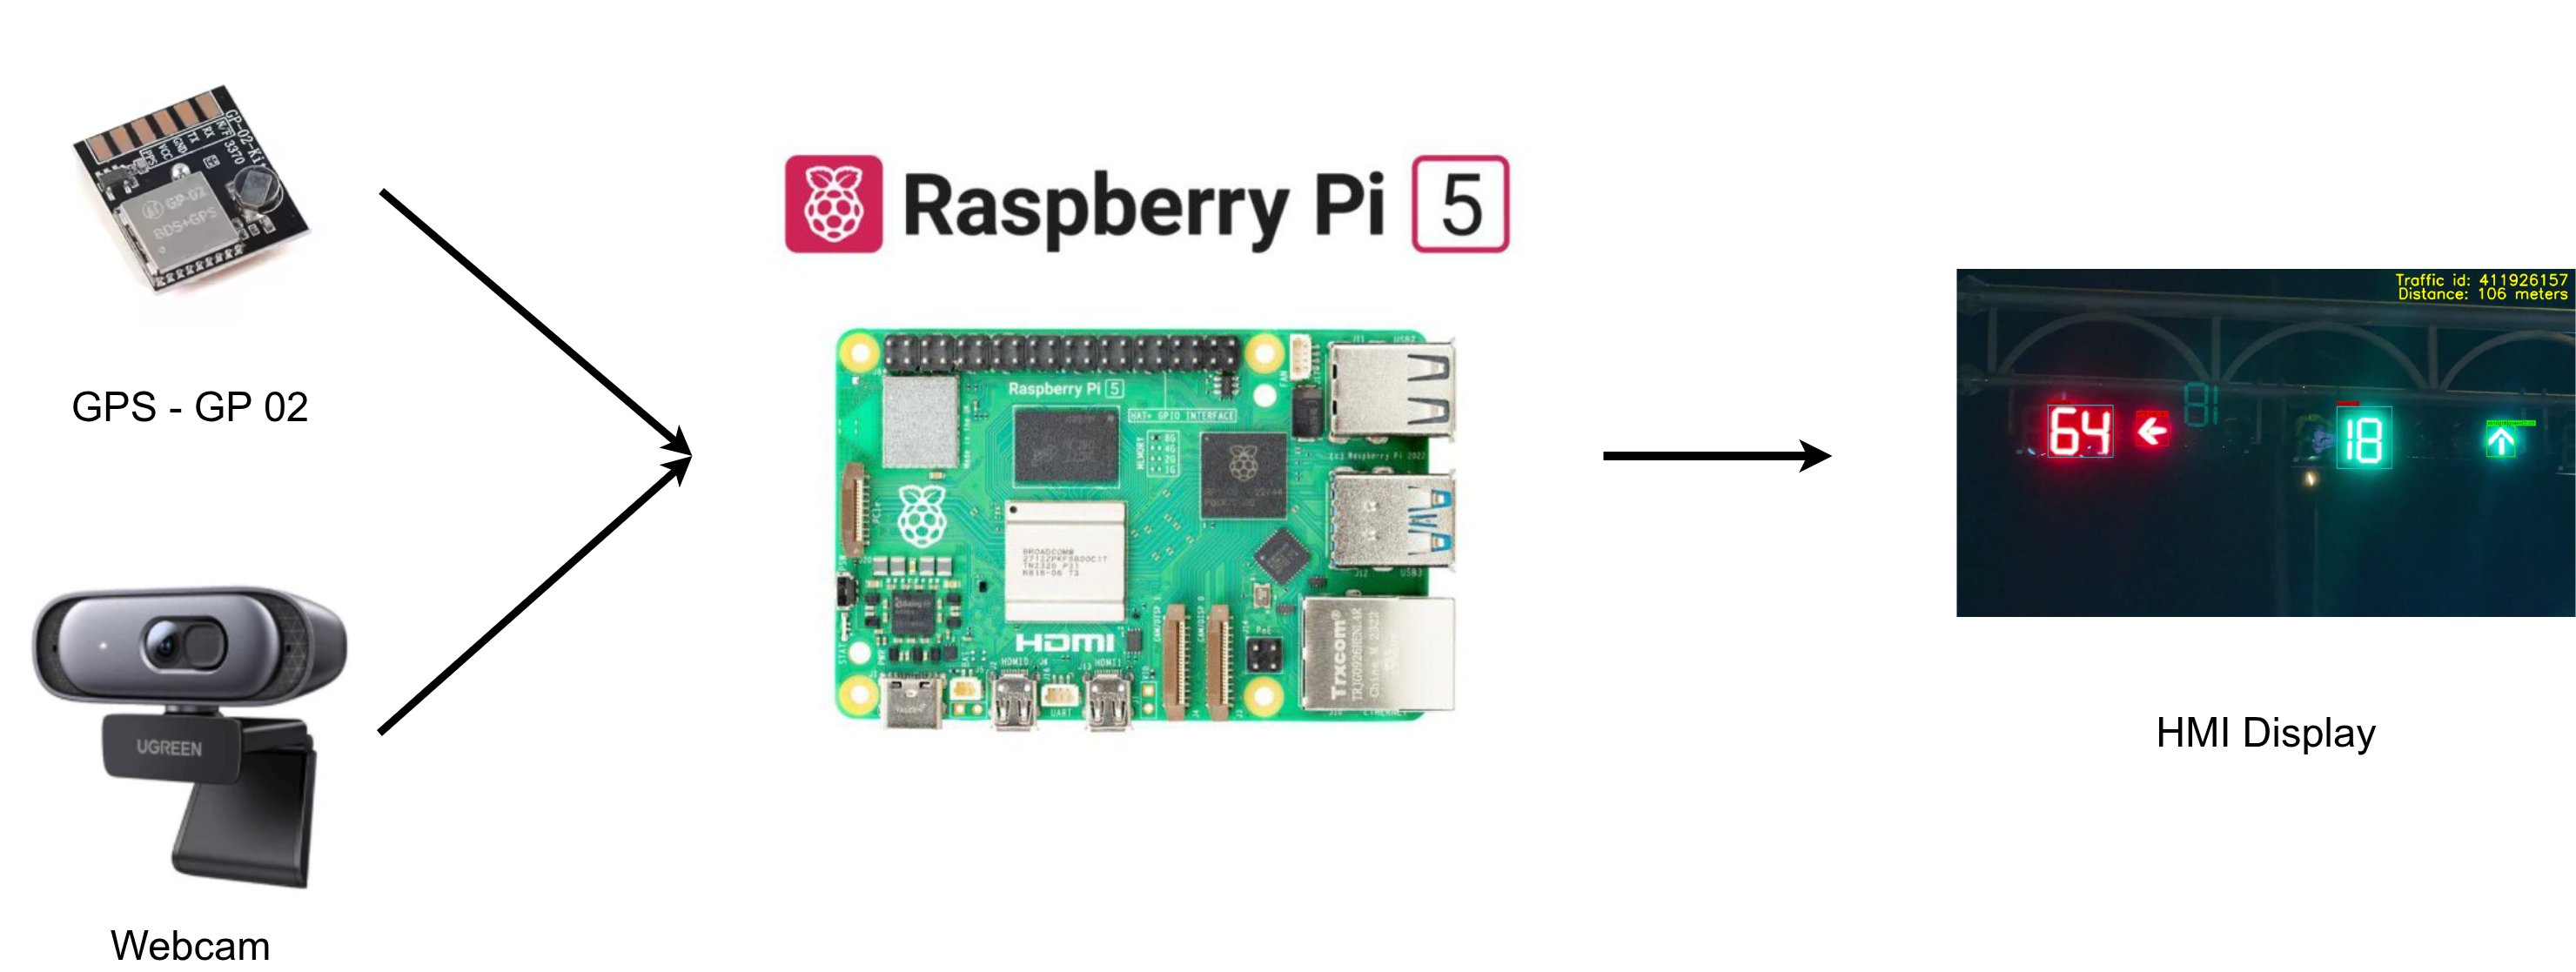
\includegraphics[width=0.8\textwidth]{Images/chapter2/hardware.png}
    \vspace{0.5cm}
    \caption{Hardware Architecture}
    \label{fig:hw_arch}
\end{figure}

\begin{itemize}
    \item \textbf{Raspberry Pi 5:} Acts as the central High-Performance Computing (HPC) unit, leveraging the Broadcom BCM2712 quad-core Arm Cortex-A76 processor clocked at 2.4GHz. This architecture delivers a \textbf{2-3x} performance boost over previous generations, providing the necessary computational overhead to execute complex Adaptive AUTOSAR applications, manage high-frequency DDS data distribution, and perform real-time edge-AI inference directly on the CPU.
    \item \textbf{USB Webcam:} Captures real-time video streams of the vehicle's surrounding environment, providing continuous visual input for the system's perception and object detection algorithms.
    \item \textbf{Ai-Thinker GP-02 GPS Module:} Acquires precise real-time geolocation data, including coordinates and velocity, which is essential for vehicle tracking and spatial awareness functions.
    \item \textbf{HMI Display:} Serves as the primary Human-Machine Interface, visually presenting critical information such as the real-time camera feed, object detection results, tracking data, and overall system status to the user.
\end{itemize}



In summary, the integration of Adaptive AUTOSAR, computer vision, AI inference via LiteRT, and GNSS-based spatial reasoning establishes the essential technical baseline for the proposed ADAS prototype. Rather than functioning as isolated technologies, the respective components form a coordinated ecosystem where software architecture, perception, localization, and physical hardware must seamlessly interact. Building upon that comprehensive background, the subsequent chapter transitions from theory to practical application. It details the exact configuration methodology, explaining how the selected frameworks are transformed into deployable AUTOSAR artifacts, trained AI models, and a reproducible execution environment.


% \input{}


\newpage
% \chapter{Configuration Adaptive AUTOSAR Project and Environment}

% Modern Advanced Driver Assistance Systems (ADAS) increasingly rely on high-performance computing, service-oriented communication, and AI-based perception algorithms to support complex driving scenarios. Functions such as traffic light recognition, object detection, and driver warning systems require not only high computational performance but also flexible software architectures that can evolve over time.

% Traditional automotive software platforms, which are primarily designed for static and tightly coupled embedded systems, are no longer sufficient to meet these requirements. These platforms typically rely on fixed signal-based communication and tightly integrated software stacks, which limit scalability and adaptability. As vehicle systems become more software-intensive and computation-heavy, especially with the integration of artificial intelligence, a more flexible execution and deployment model is required.

% To address these challenges, AUTOSAR introduced the \textit{Adaptive Platform}. Unlike the Classic Platform, the Adaptive Platform supports dynamic deployment, service-oriented architectures, and execution on high performance computing units using POSIX compliant operating systems. This allows automotive applications to adopt modern software engineering practices while still complying with automotive safety and reliability requirements.

% This chapter presents the configuration process of an Adaptive AUTOSAR project and its execution environment. The focus is on how system artefacts, software components, and deployment descriptions are organized and integrated following the Adaptive AUTOSAR Methodology. Compared to classical development flows, the Adaptive approach emphasizes incremental refinement, explicit artefact dependencies, and a clear separation between design, implementation, and deployment phases. This structured methodology is particularly suitable for complex ADAS systems, where multiple software components must interact dynamically at runtime.

% In addition, this chapter describes the configuration and training of the YOLO-MobileNetv4 model used for perception tasks, as well as the cross-compilation of the LiteRT framework for integration into the Adaptive AUTOSAR environment. Finally, a Docker, which based development environment is introduced to ensure reproducibility, portability, and consistency across different development stages.

% The remainder of this chapter is organized as follows. Section~\ref{sec:adaptive_methodology} introduces the Adaptive AUTOSAR methodology and its knowledge base. The configuration and training process of YOLO-MobileNetv4 is discussed afterward. The cross-compilation workflow for the LiteRT framework is then presented, followed by the setup of the Adaptive AUTOSAR Docker environment.

% % TODO: Insert a high-level workflow figure showing Methodology -> AI Model -> Cross Compilation -> Docker Environment

% \section{Adaptive AUTOSAR Methodology}
% \label{sec:adaptive_methodology}
% \subsection{Knowledge Base}

The Adaptive AUTOSAR Methodology is founded on a structured and comprehensive knowledge base that defines how automotive software systems are specified, designed, implemented, and deployed. This knowledge base is standardized by AUTOSAR and documented in the Methodology for Adaptive
Platform (Version R22-11)\cite{AUTOSAR_TR_AdaptiveMethodology_R22-11}. Its purpose is to provide a consistent methodological framework that can be applied across different organizations, toolchains, and system architectures.

The knowledge base defines a set of development phases together with the artefacts that are produced and consumed in each phase. By explicitly modeling artefact relationships, the methodology ensures traceability throughout the system lifecycle, from early architectural descriptions to deployable software units. Such traceability is a key requirement for large-scale automotive software systems, where changes at one abstraction level must be systematically reflected at others.

At the core of the Adaptive AUTOSAR Methodology are the \textit{Method Content Packages}. Each Method Content Package represents a coherent development stage and specifies:
\begin{itemize}
    \item The input artefacts required to initiate the phase,
    \item The output artefacts that are produced or extended,
    \item And the refinement relations between artefacts across phases.
\end{itemize}

This structure supports incremental and iterative development, allowing architectural decisions to be refined step by step while preserving consistency between abstraction levels.

% TODO: Insert figure illustrating Adaptive AUTOSAR Method Content Packages
\begin{figure}[h]
    \centering
    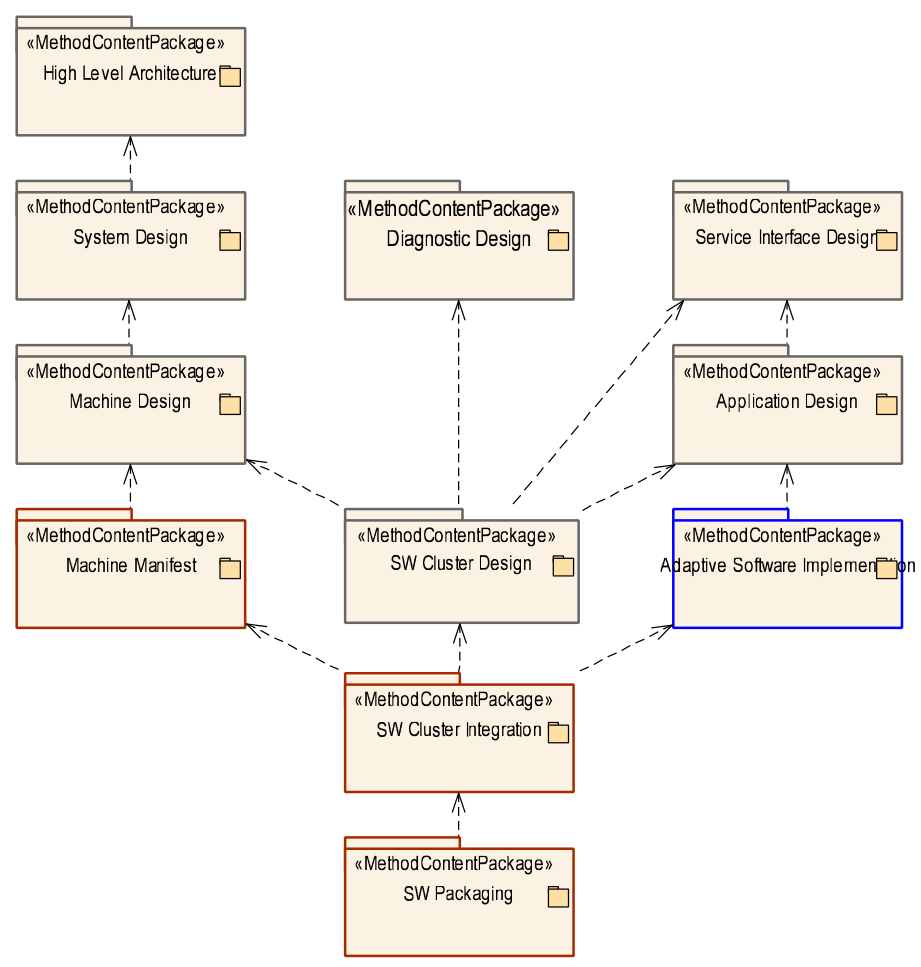
\includegraphics[width=0.75\textwidth]{Images/chap3/image_methodology/knowledgeBase/AdaptiveMethodology.png}
    \vspace{0.5cm}
    \caption{Adaptive Methodology}
    \label{fig:adap_methodology}
\end{figure}

% \subsubsection{High Level Architecture}

% % Figure before explanation
% \begin{figure}[H] % Dùng ht (here, top) là chuẩn nhất
%     \centering
%     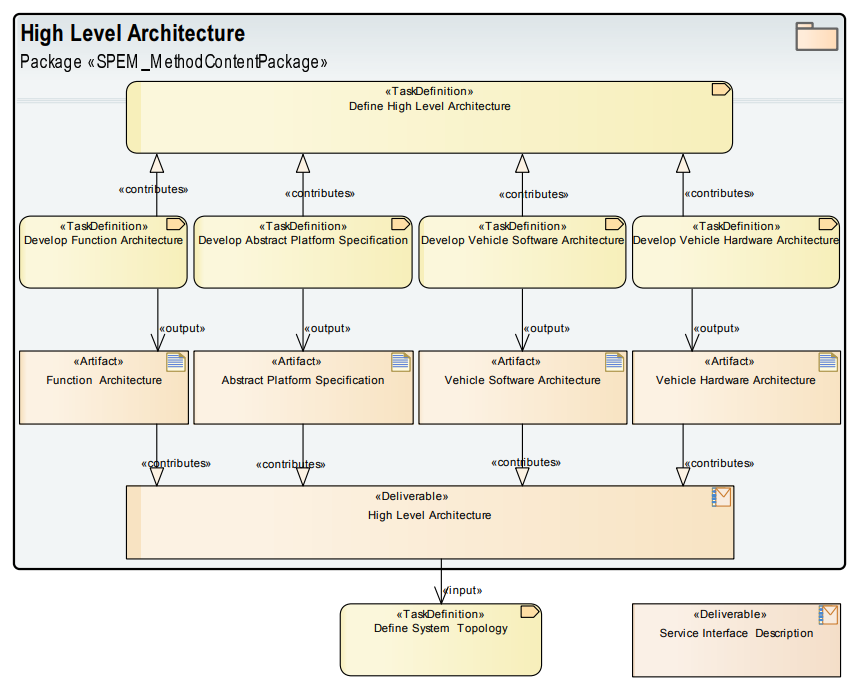
\includegraphics[width=0.75\textwidth]{Images/chap3/image_methodology/knowledgeBase/HLA.png}
%     \vspace{0.5cm}
%     \caption{High Level Architecture in Adaptive AUTOSAR Methodology}
%     \label{fig:hla_architecture} % Đã đổi tên nhãn để không trùng
% \end{figure}

% The High Level Architecture represents the initial and most abstract architectural view within the Adaptive AUTOSAR Methodology. Its primary purpose is to establish a common architectural foundation for the vehicle E/E system before detailed system design and implementation activities are performed.

% As illustrated in Figure~\ref{fig:hla_architecture}, the High Level Architecture is defined through a set of coordinated architectural tasks that collectively contribute to a unified architectural deliverable. These tasks include the development of the Function Architecture, the Abstract Platform Specification, the Vehicle Software Architecture, and the Vehicle Hardware Architecture. Each task addresses a specific architectural concern while remaining independent of concrete implementation decisions.

% The Function Architecture focuses on identifying and structuring the system functions and their logical relationships. It describes what the system is expected to do, without specifying how or where these functions are executed. In parallel, the Abstract Platform Specification defines the abstract execution environment and platform capabilities required by the software, serving as a conceptual bridge between functional requirements and platform realization.

% The Vehicle Software Architecture describes the high level organization of software elements within the vehicle, including major software partitions and their responsibilities. Complementarily, the Vehicle Hardware Architecture captures the high-level hardware structure of the system, including computing units and their relationships, without binding the architecture to specific hardware components.

% The outputs of these architectural tasks are formalized as architectural artefacts. These artefacts collectively contribute to the High-Level Architecture deliverable, which serves as a key input for subsequent methodology phases. In particular, the High Level Architecture provides the architectural context required for defining the system topology and service interface descriptions in later stages.

% By separating functional, software, hardware, and platform concerns at this early stage, the High Level Architecture supports architectural clarity, scalability, and consistency. It ensures that subsequent design and integration activities are grounded in a coherent and well-structured architectural vision.


% \subsubsection{System Design}

% % Figure before explanation
% \begin{figure}[H] % Dùng ht (here, top) là chuẩn nhất
%     \centering
%     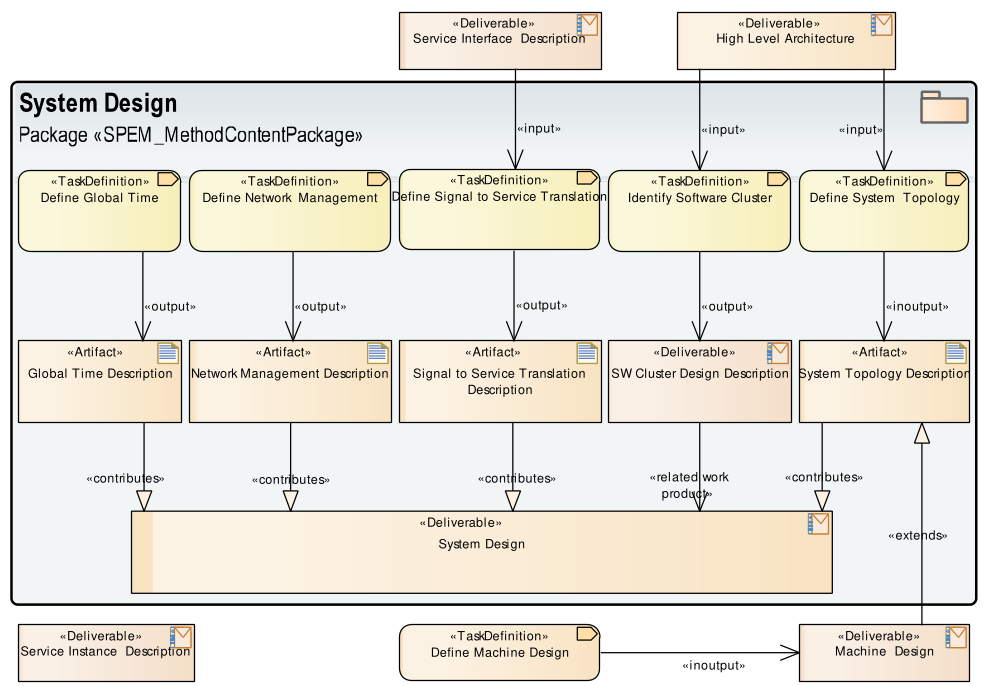
\includegraphics[width=0.75\textwidth]{Images/chap3/image_methodology/knowledgeBase/systemDesign.png}
%     \vspace{0.5cm}
%     \caption{System Design in Adaptive AUTOSAR Methodology}
%     \label{fig:system_design} % Đã đổi tên nhãn để không trùng
% \end{figure}

% The System Design phase refines the architectural concepts established in the High-Level Architecture into a more concrete and structured system-level description. Its primary objective is to define how software elements, communication mechanisms, and system resources are organized and coordinated within the Adaptive AUTOSAR environment.

% As illustrated in the System Design package, this phase consumes key architectural deliverables, including the High Level Architecture and the Service Interface Description, as inputs. Based on these inputs, a set of dedicated design tasks is performed to derive detailed system artefacts that collectively form the System Design deliverable.

% One of the central tasks in this phase is the definition of global timing concepts. The \textit{Define Global Time} task establishes a common time base for the system, which is essential for coordinating distributed software execution and ensuring temporal consistency across different system elements. The resulting Global Time Description contributes to the overall System Design by providing a unified temporal reference.

% In parallel, the \textit{Define Network Management} task specifies how communication networks are controlled and supervised at the system level. This task produces the Network Management Description, which defines network states, transitions, and management strategies. These definitions support reliable communication and controlled system behavior during startup, operation, and shutdown phases.

% Another key task within this phase is the \textit{Define Signal to Service Translation}. This task addresses the mapping between signal-oriented communication and service-oriented communication. The resulting Signal to Service Translation Description enables interaction between system elements that rely on different communication paradigms, ensuring compatibility and interoperability within the Adaptive Platform.

% The System Design phase also includes the identification of software clusters through the \textit{Identify Software Cluster} task. Software clusters group related software elements into coherent deployment units. The resulting Software Cluster Design Description serves as an important intermediate artefact that supports later integration and deployment activities.

% Furthermore, the \textit{Define System Topology} task specifies how system elements are arranged and connected. The System Topology Description captures function groups, network endpoints, and their relationships. This description provides a structural view of the system and serves as a foundation for subsequent deployment and machine-specific design steps.

% All artefacts generated during these tasks contribute to the System Design deliverable. Together, they establish a consistent and detailed system level specification that bridges the gap between high level architectural concepts and later design phases. The System Design deliverable also provides essential inputs for related activities, such as service instance specification and machine design.

% By consolidating timing, communication, clustering, and topology aspects, the System Design phase ensures that the Adaptive AUTOSAR system is coherently structured and ready for further refinement in subsequent methodology stages.


% % TODO: Insert system topology and communication overview figure

% \subsubsection{Service Interface Design}

% % Figure before explanation
% \begin{figure}[H] % Dùng ht (here, top) là chuẩn nhất
%     \centering
%     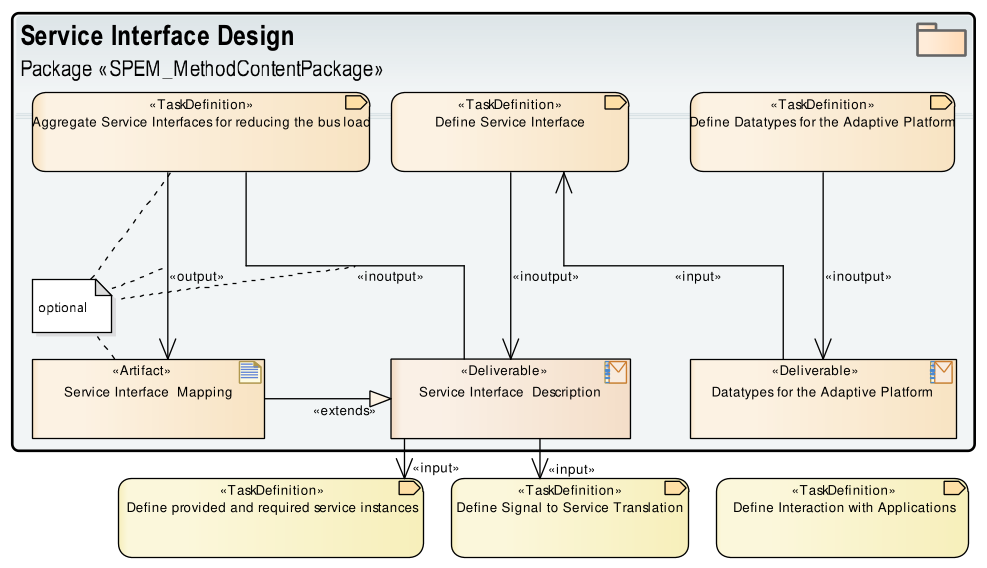
\includegraphics[width=0.75\textwidth]{Images/chap3/image_methodology/knowledgeBase/serviceInterfaceDesign.png}
%     \vspace{0.5cm}
%     \caption{Service Interface Design in Adaptive AUTOSAR Methodology}
%     \label{fig:service_interface_design} % Đã đổi tên nhãn để không trùng
% \end{figure}

% The Service Interface Design defines how Service Interface Descriptions are created, refined, and reused within the Adaptive AUTOSAR development process. This usage scenario explains the sequence of design activities and their associated work products, as illustrated in Figure~\ref{fig:service_interface_design}, focusing on the relationship between service interfaces, datatypes, and interface mappings.

% According to the methodology, Service Interface Descriptions can be obtained through two main usage scenarios: create or change use cases and reuse use cases. These scenarios are not isolated phases but can be integrated into both system design and application design activities, depending on the development context.

% In create or change use cases, Service Interface Descriptions are derived by performing a set of tailored tasks. The central task is the definition of a service interface, which specifies the service operations, events, and communication semantics. In parallel, datatypes for the Adaptive Platform are defined or refined to describe the data exchanged through the service interface. These tasks may be supported by the aggregation of service interfaces, which aims to reduce communication bus load by grouping related service elements when appropriate. The resulting Service Interface Mapping artefact optionally extends the Service Interface Description by documenting how aggregated or related interfaces are organized.

% This scenario is typically applied in a top-down development approach, where architectural or system level considerations drive the definition of service interfaces and datatypes. The outputs of these tasks include the Service Interface Description and the Datatypes for the Adaptive Platform, which together form the primary deliverables of this design stage.

% In reuse use cases, existing Service Interface Descriptions are adopted as inputs with minimal modification. In this case, service interfaces and their associated datatypes are reused from predefined specifications or existing libraries. If required, datatypes may be extended to align with the specific system context. This scenario is commonly applied in a bottom-up development approach and supports efficient reuse across different projects.

% The resulting work products of both scenarios are tailored Service Interface Descriptions and corresponding Datatype Descriptions. These deliverables serve as inputs for subsequent design activities, such as the definition of provided and required service instances, signal-to-service translation, and the specification of interactions with applications.

% By explicitly structuring the creation, aggregation, mapping, and reuse of service interfaces, the Service Interface Design usage scenario ensures consistency, modularity, and reusability of service definitions within the Adaptive AUTOSAR methodology.

% \subsubsection{Application Design}

% % Figure before explanation
% \begin{figure}[H]
%     \centering
%     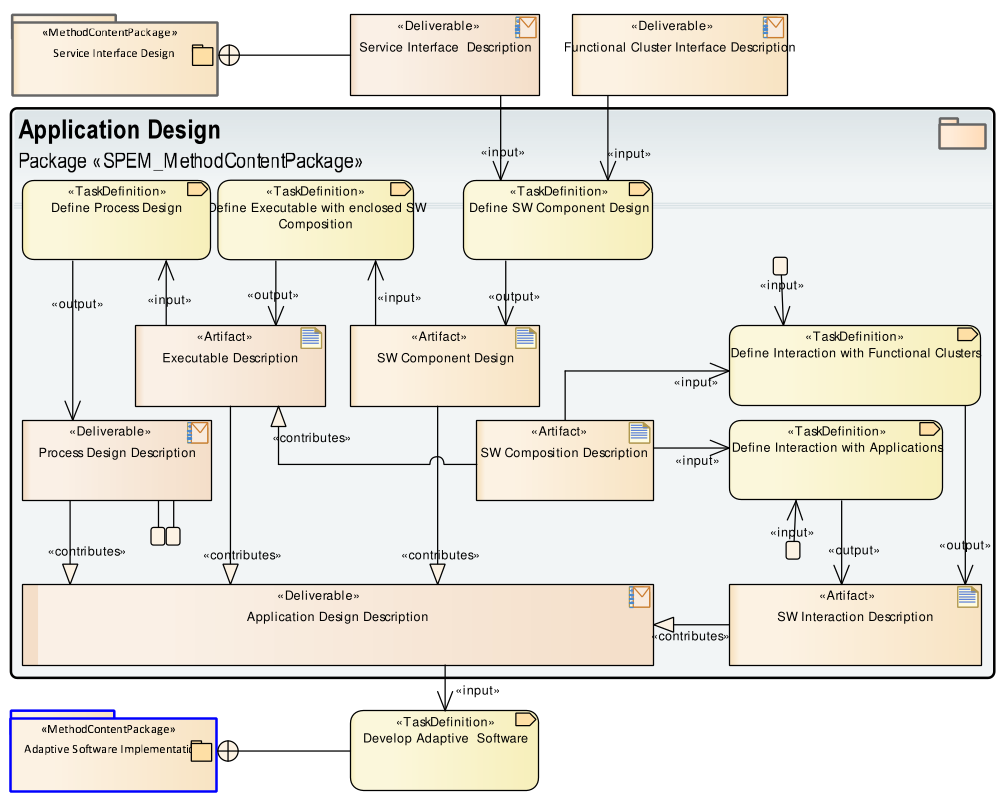
\includegraphics[width=0.75\textwidth]{Images/chap3/image_methodology/knowledgeBase/applicationDesign.png}
%     \vspace{0.5cm}
%     \caption{Application Design in Adaptive AUTOSAR Methodology}
%     \label{fig:application_design}
% \end{figure}

% The Application Design phase refines the outcomes of system level and service-level design into a detailed specification of executable software structures. Its primary objective is to describe how software components are organized, instantiated, and interconnected during runtime execution within the Adaptive AUTOSAR Platform.

% As shown in Figure~\ref{fig:application_design}, this phase takes the Service Interface Description and the Functional Cluster Interface Description as inputs. Based on these artefacts, a set of closely related design activities is carried out, leading to the definition of the overall Application Design Description.

% One of the key activities in this phase is \textit{Define Software (SW) Component Design}. This activity results in the SW Component Design artefact, which specifies the internal structure of software components and their interaction endpoints. These endpoints are expressed through software component (SWC) ports instantiating specific port interfaces at either the application level or the platform level. The SW Component Design establishes the structural basis required for subsequent composition and interaction definitions.

% Another essential activity is \textit{Define Executable with enclosed SW Composition}, which determines how software components are assembled into executable units. Its outcome is the Executable Description, including the SW Composition Description. This description identifies the software components contained within an executable and defines their structural relationships. The execution of this activity requires that all referenced SW Component Designs are already available.

% The runtime realization of executables is addressed by the \textit{Define Process Design} activity. The resulting Process Design Description represents a design time abstraction of the operating system process responsible for instantiating and starting a specific executable. This activity builds upon the Executable Description and provides the link between executable definitions and their runtime execution context.

% Interaction which related aspects are specified through the activities \textit{Define Interaction with Applications} and \textit{Define Interaction with Functional Clusters}. Together, these activities produce the SW Interaction Description, which captures all interaction configurations that are relevant at design time. This includes interactions between application-level software components as well as interactions with platform-level functional clusters. The definition of these interactions depends on the availability of the Process Design Description, the corresponding Executable Description with its SW Composition Description, and the interaction endpoints defined in the SW Component Designs.

% All artefacts produced during the Application Design phase contribute to the Application Design Description deliverable. This deliverable consolidates software component definitions, executable compositions, process abstractions, and interaction configurations into a consistent and comprehensive design representation.

% The activities within the Application Design phase are interdependent and may be performed in an order that best fits the project context. Although the primary focus of this phase is on application-level software, the same design principles and activities may also be applied to platform-level software, particularly when port and port interface concepts are supported.

% The resulting Application Design Description serves as a fundamental input for the subsequent Adaptive Software Implementation phase, where the defined software structures are realized as executable software.

% \subsubsection{Adaptive Software Implementation}

% % Figure before explanation
% \begin{figure}[H]
%     \centering
%     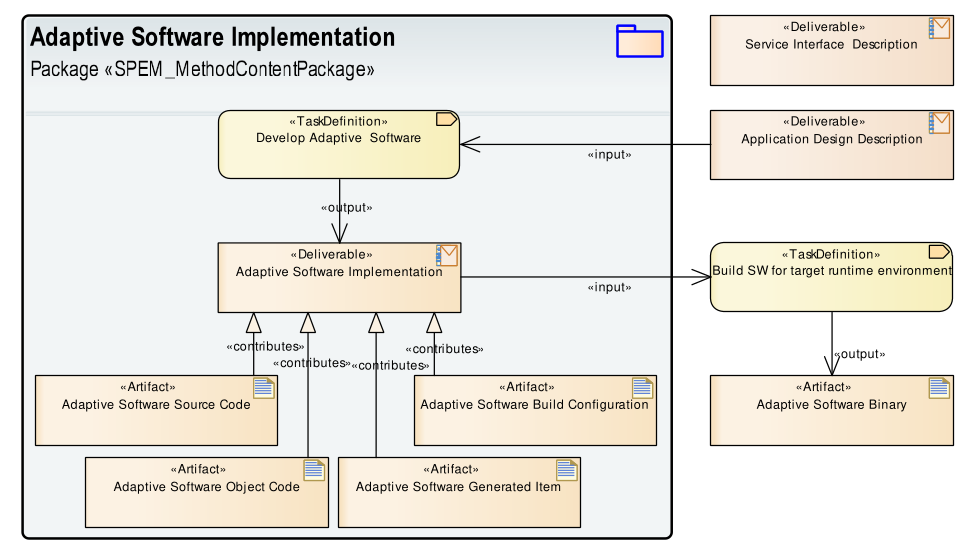
\includegraphics[width=0.75\textwidth]{Images/chap3/image_methodology/knowledgeBase/softwareImplementation.png}
%     \vspace{0.5cm}
%     \caption{Adaptive Software Implementation in Adaptive AUTOSAR Methodology}
%     \label{fig:software_implementation}
% \end{figure}

% The Adaptive Software Implementation phase addresses the realization of software defined during the preceding design stages. Its purpose is to transform the Application Design Description into concrete software artefacts that can be integrated and executed within the Adaptive AUTOSAR runtime environment.

% As depicted in Figure~\ref{fig:software_implementation}, this phase is initiated once the Service Interface Description and the Application Design Description are available. These deliverables provide the necessary interface definitions and structural specifications required to start the implementation activities.

% The central activity of this phase is \textit{Develop Adaptive Software}. This activity encompasses the development of application level and/or platform level Adaptive Software and may include analysis, detailed design, implementation, and testing activities. The development process relies on Adaptive Software Generated Items, such as service proxies and service skeletons, which are derived from service interface definitions and support the implementation of communication ports and port interfaces.

% Depending on the availability of the Adaptive Software Build Configuration, the development process follows different realization paths. When the build configuration is known in advance, software components can be compiled by the developer, and Adaptive Software Object Code can be delivered directly. In contrast, if the build configuration is not available, the developer provides Adaptive Software Source Code, and the compilation is performed later by the integrator.

% The artefacts produced during software development include Adaptive Software Source Code, Adaptive Software Object Code, Adaptive Software Generated Items, and the Adaptive Software Build Configuration. Together, these artefacts contribute to the Adaptive Software Implementation deliverable, which represents the complete implementation result prepared for integration.

% The transformation of the implementation into deployable form is addressed by the activity \textit{Build software (SW) for target runtime environment}. This activity consumes the Adaptive Software Implementation and produces the Adaptive Software Binary. The binary represents the executable form of the software that is suitable for deployment on the target machine and runtime environment.

% Throughout this phase, both application level and platform level Adaptive Software are treated consistently. Each executable requires a main function and an execution manifest, enabling instantiation and deployment within the Adaptive AUTOSAR execution framework.

% The Adaptive Software Implementation deliverable produced in this phase serves as the handover point between software development and integration. It provides the necessary implementation artefacts for subsequent software cluster integration, packaging, and deployment activities.

% \subsubsection{Diagnostic Design}

% % Figure before explanation
% \begin{figure}[H]
%     \centering
%     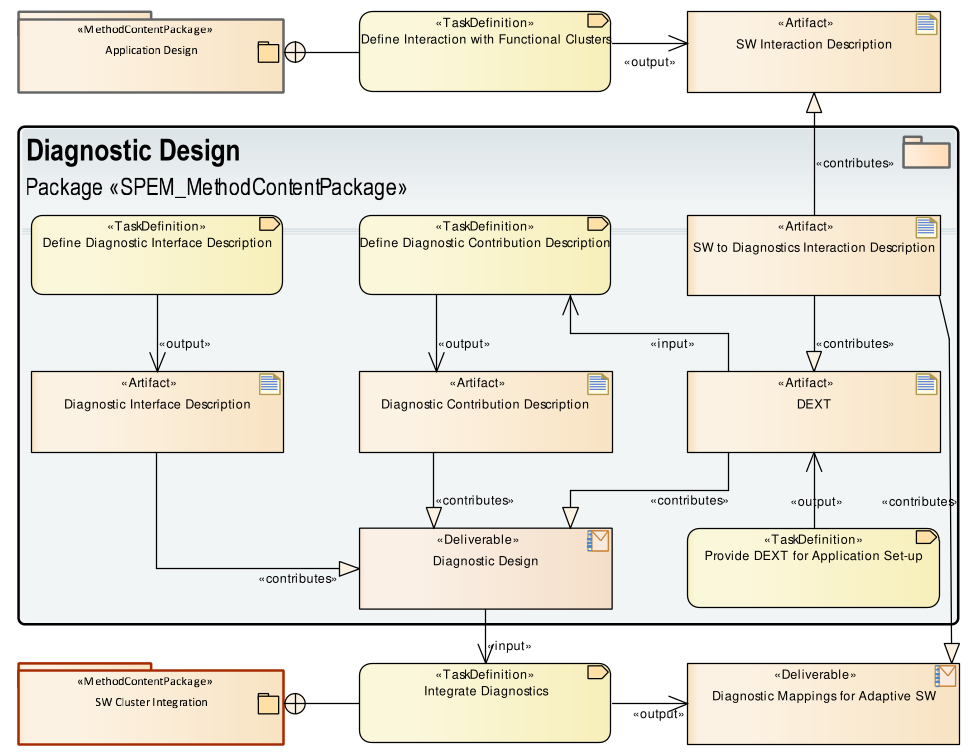
\includegraphics[width=0.75\textwidth]{Images/chap3/image_methodology/knowledgeBase/diagDesign.png}
%     \vspace{0.5cm}
%     \caption{Diagnostic Design in Adaptive AUTOSAR Methodology}
%     \label{fig:diag_design}
% \end{figure}

% The Diagnostic Design phase focuses on defining how diagnostic information is associated with the software structures of the Adaptive AUTOSAR system. Its main objective is to prepare diagnostic which related artefacts that enable consistent monitoring, reporting, and interaction with the diagnostic manager during system operation.

% As shown in Figure~\ref{fig:diag_design}, Diagnostic Design builds on results obtained during the Application Design phase, particularly the SW Interaction Description that captures interactions with functional clusters. These interaction definitions provide the context required to specify diagnostic interfaces and mappings in a systematic manner.

% The activity \textit{Define Diagnostic Interface Description} establishes the diagnostic interfaces that adaptive software components expose for diagnostic purposes. The resulting Diagnostic Interface Description specifies diagnostic port interfaces and their characteristics, allowing diagnostic managers to access diagnostic which relevant data and services in a standardized way.

% Complementing this, the activity \textit{Define Diagnostic Contribution Description} identifies the diagnostic content contributed by software elements within a given context. The Diagnostic Contribution Description determines which parts of the diagnostic configuration are relevant for specific executables or software clusters and are intended to be processed by the diagnostic manager.

% Diagnostic resources and configuration data are collected and structured through the activity \textit{Provide DEXT for Application Setup}. This activity produces or extends the Diagnostic Extract (DEXT), which contains diagnostic resources such as diagnostic data identifiers, diagnostic events, enable conditions, and operation cycles. The DEXT acts as a reusable container for diagnostic configuration and may cover multiple executables, diagnostic managers, and software clusters across the vehicle.

% The association between diagnostic resources and software interaction endpoints is captured in the SW to Diagnostics Interaction Description. This artefact specifies how diagnostic information is mapped to software component ports at design time and contributes both to the Diagnostic Design deliverable and to the DEXT. It represents an intermediate form of diagnostic mappings that is refined during later integration steps.

% All artefacts produced during this phase, including the Diagnostic Interface Description, Diagnostic Contribution Description, SW to Diagnostics Interaction Description, and the DEXT, collectively contribute to the Diagnostic Design deliverable. This deliverable provides a consolidated view of the diagnostic configuration that is prepared for further integration activities.

% The Diagnostic Design deliverable is subsequently used as input for the \textit{Integrate Diagnostics} activity during Software Cluster Integration. In that phase, diagnostic mappings are finalized by associating diagnostic resources with concrete executable instances and operating system processes, resulting in the Diagnostic Mappings for Adaptive Software.

% By structuring diagnostic interface definition, contribution specification, and resource extraction as distinct but related activities, the Diagnostic Design phase supports a clear and maintainable diagnostic configuration process within the Adaptive AUTOSAR methodology.

% \subsubsection{Machine Design}

% % Figure before explanation
% \begin{figure}[H]
%     \centering
%     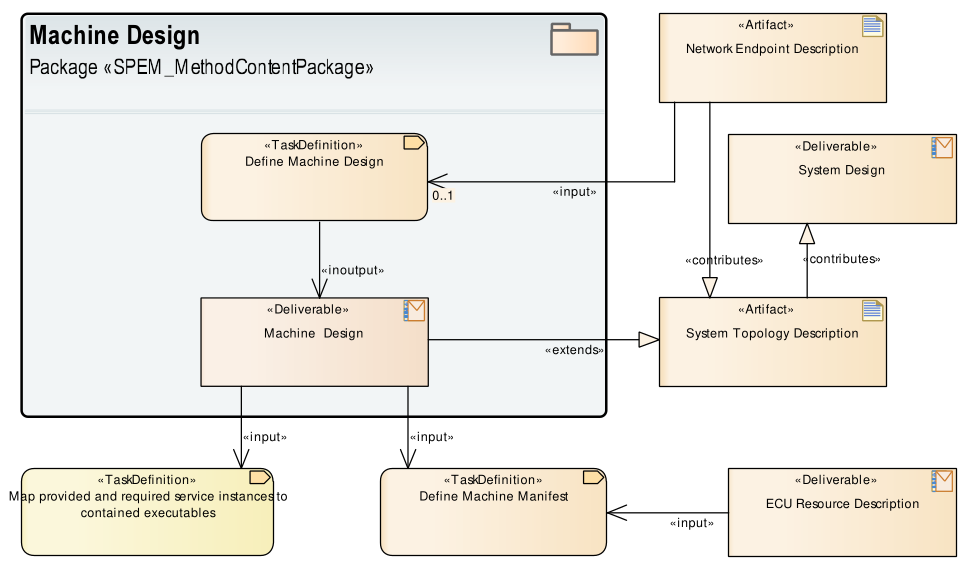
\includegraphics[width=0.75\textwidth]{Images/chap3/image_methodology/knowledgeBase/machineDesign.png}
%     \vspace{0.5cm}
%     \caption{Machine Design in Adaptive AUTOSAR Methodology}
%     \label{fig:machine_design}
% \end{figure}

% The Machine Design phase addresses the specification of a machine from a communication and deployment standpoint within the Adaptive AUTOSAR Platform. Its aim is to describe the characteristics of a machine that are required for software execution and service communication, taking into account system level topology information and the capabilities of the target ECU.

% Figure~\ref{fig:machine_design} provides an overview of the activities involved in this phase. The core activity, \textit{Define Machine Design}, derives a machine-oriented configuration by using network endpoint information defined during System Design. In particular, the System Topology Description and the associated Network Endpoint Description supply the addressing and service discovery parameters needed to shape the communication behavior of the machine.

% The result of this activity is captured in the Machine Design deliverable. This deliverable augments the existing System Topology Description by introducing machine specific communication constraints and requirements. At this stage, the design remains independent of a concrete hardware realization and represents a prospective configuration for a machine.

% Beyond defining communication aspects, the Machine Design also provides the basis for associating software deployment elements with the machine. Through the activity \textit{Map provided and required service instances to contained executables}, service instances are linked to executables that are intended to run on the machine. This association clarifies how services are realized by software units within the machine context.

% The adaptation of the machine configuration to a specific hardware platform is performed in a subsequent activity, \textit{Define Machine Manifest}. This activity combines the Machine Design with the ECU Resource Description, which details the resources and limitations of the target ECU. The outcome is the Machine Manifest, representing a machine configuration that is fully aligned with the characteristics of a real ECU.

% From a methodological viewpoint, machine configuration follows a two-step process. The first step establishes the communication structure of a machine and yields the Machine Design. This step may be carried out in a top-down manner, guided by an existing System Design, or in a bottom-up manner, where machine-specific communication definitions are created locally and may later contribute to the overall system topology.

% The second step focuses on hardware-specific realization and results in the Machine Manifest. This separation between prospective machine definition and ECU specific configuration supports a clear allocation of responsibilities between system designers and integrators, while maintaining flexibility during system integration.

% \subsubsection{Machine Manifest}

% % Figure before explanation
% \begin{figure}[H]
%     \centering
%     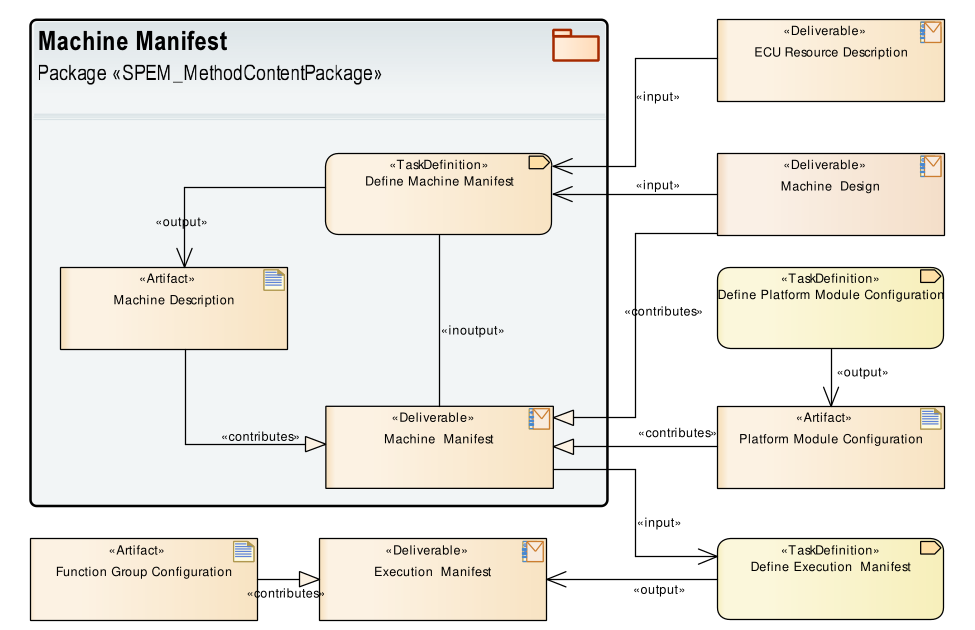
\includegraphics[width=0.75\textwidth]{Images/chap3/image_methodology/knowledgeBase/machineManifest.png}
%     \vspace{0.5cm}
%     \caption{Machine Manifest in Adaptive AUTOSAR Methodology}
%     \label{fig:machine_manifest}
% \end{figure}

% The Machine Manifest phase specifies the final configuration of a machine that is ready to be deployed on a concrete ECU within the Adaptive AUTOSAR Platform. Its purpose is to consolidate communication-related design results with hardware resource information and platform-specific configurations into a single, deployment ready description.

% Figure~\ref{fig:machine_manifest} outlines the activities and work products involved in this phase. The primary activity, \textit{Define Machine Manifest}, is initiated once the Machine Design and the ECU Resource Description are available. While the Machine Design provides a prospective view of the machine configuration, the ECU Resource Description defines the concrete hardware resources offered by the target ECU.

% The outcome of this activity is the Machine Manifest deliverable. The Machine Manifest integrates several key elements. First, it contains the Machine Description, which describes the available hardware resources of the ECU, such as processing units, memory resources, sensors, actuators, and other relevant hardware elements. This information is derived from the ECU Resource Description and tailored to the specific machine instance.

% Second, the Machine Manifest incorporates the Machine Design, thereby preserving the communication structure and network-related configuration that was defined during the Machine Design phase. This ensures that the communication requirements identified earlier are consistently realized on the target ECU.

% In addition, platform-specific aspects are addressed through the activity \textit{Define Platform Module Configuration}. This activity produces Platform Module Configuration artefacts, which specify the machine-specific configuration of Adaptive Platform modules. These configurations may include the operating system setup, platform services such as network management and diagnostics, as well as foundation modules like logging and tracing. The resulting Platform Module Configurations contribute directly to the Machine Manifest.

% The configuration of software execution is captured by the activity \textit{Define Execution Manifest}. This activity produces the Execution Manifest, which specifies which executables are instantiated on the machine and how they are mapped to processes. The Execution Manifest may also include Function Group Configurations that control the activation and deactivation of software elements. The Execution Manifest contributes to the Machine Manifest by defining the runtime behavior of software on the machine.

% From a process perspective, the Machine Manifest is typically assembled in an incremental manner. Communication-related configurations originating from the Machine Design are collected first, followed by the integration of hardware resource descriptions and platform module configurations. As additional configuration information becomes available, the Machine Manifest may be iteratively extended and refined.

% By consolidating machine-specific communication settings, hardware resource descriptions, platform module configurations, and execution information, the Machine Manifest provides a complete and consistent representation of a machine that is ready for deployment within the Adaptive AUTOSAR ecosystem.

% \subsubsection{Software Cluster Design, Integration, and Packaging}

% The phases of Software Cluster Design, Software Cluster Integration, and Software Packaging together form the final preparation steps that transform implemented Adaptive AUTOSAR software into deployable units. These phases consolidate design results, integrate software components with their configurations, and prepare complete software packages for deployment on target machines.

% Software Cluster Design focuses on defining logical groupings of software elements that belong together from a deployment and lifecycle perspective. A software cluster typically bundles application level software, required platform services, and related configuration artifacts into a coherent unit. The purpose of this phase is not to define execution details, but to establish clear cluster boundaries, dependencies, and responsibilities that simplify later integration and deployment activities.

% Based on the cluster definitions, Software Cluster Integration performs the concrete assembly of software and configuration artifacts. During this phase, Adaptive Software Implementations, design descriptions, machine which related information, and diagnostic configurations are brought together and checked for consistency. Integration activities refine execution which related information, such as the association of executables with machines and processes, and complete interaction and diagnostic mappings that could only be finalized once all involved elements are known. As a result, the integrated software cluster represents a consistent and executable view of the system for a specific deployment context.

% Software Packaging completes the workflow by preparing integrated software clusters for delivery and deployment. In this phase, all relevant artifacts, such as software binaries, manifests, configuration files and generated items which are collected and organized into software packages. These packages are structured in a way that supports deployment, update, and lifecycle management, while preserving a clear separation between different software clusters.

% By combining cluster definition, integration, and packaging into a structured workflow, these phases provide a clear transition from implemented software to deployable units. This approach supports modularity, reuse, and scalable integration, which are essential characteristics of the Adaptive AUTOSAR methodology.

% \subsubsection{Summary}

% This section has presented an overview of the Adaptive AUTOSAR knowledge base and its role in structuring the development of complex automotive software systems. The methodology defines a clear sequence of development phases, each supported by well-defined artefacts and responsibilities.

Starting from high-level architectural descriptions, the methodology guides the refinement of system structure, service interfaces, application design, and software implementation. Subsequent phases address diagnostics, machine-specific configuration, and the preparation of software for deployment. Each phase builds upon the results of previous stages, ensuring consistency and traceability throughout the development process.

By explicitly modeling artefact dependencies and separating design, implementation, integration, and deployment concerns, the Adaptive AUTOSAR Methodology supports systematic system development. This approach improves scalability, facilitates reuse, and simplifies integration in large and evolving software systems.

The following section explains how the most important Method Content Packages are configured in this project and how they are refined into concrete Adaptive AUTOSAR artefacts.

% Overall, the knowledge base provides a solid methodological foundation for configuring and deploying Adaptive AUTOSAR systems. It enables a structured transition from abstract system concepts to deployable software units while maintaining clarity and consistency across the entire system lifecycle.


\subsection{Project Methodology}

In this project, the Adaptive AUTOSAR system is developed using the \texttt{Autosar.io} tool provided by PopcornSAR. Autosar.io is a configuration-oriented modeling environment that allows users to systematically define and organize an Adaptive AUTOSAR project through a set of well-structured design sections. Instead of focusing on source code implementation, the tool guides users to configure machines, services, and applications by following the standard Adaptive AUTOSAR modeling workflow.

\begin{figure}[H]
    \centering
    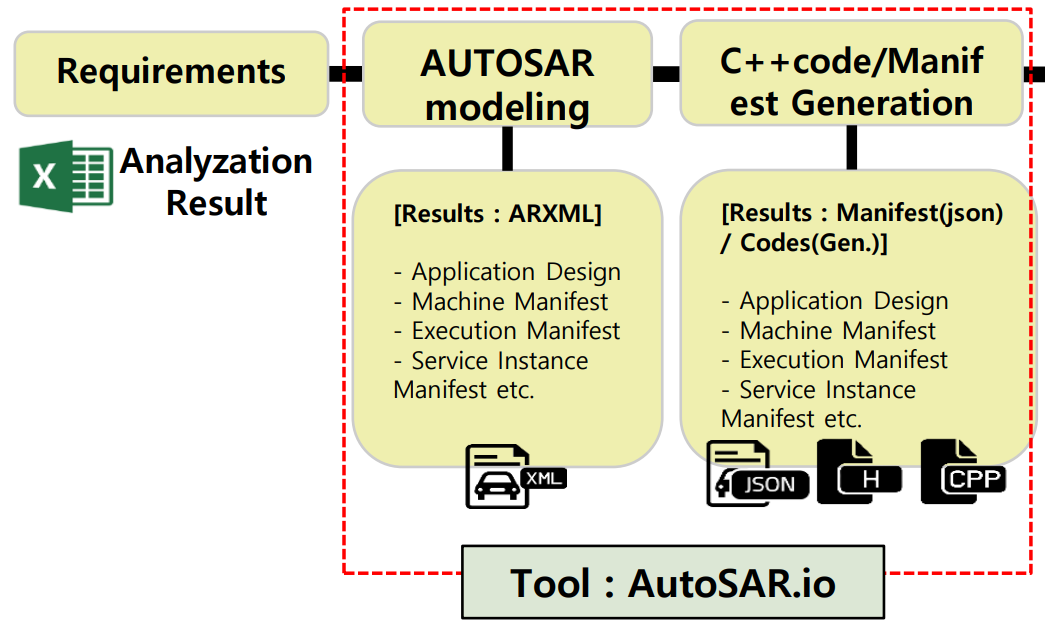
\includegraphics[width=0.75\textwidth]{Images/toolchains/autosario.png}
    \vspace{0.5cm}
    \caption{Autosar.io tool supporting configuration workflow for Adaptive AUTOSAR systems}
    \label{fig:autosario}
\end{figure}

Autosar.io provides dedicated design views that correspond directly to the configuration steps presented in this section, including Machine Design and Machine Manifest creation, Service Interface Design and Mapping, and Adaptive Application Design. Through these views, users can specify network endpoints, service discovery parameters, service interfaces, service instances, application executables, processes, startup behavior, and process-to-machine mappings. Each configuration step produces AUTOSAR-compliant artifacts such as ARXML descriptions and manifests, ensuring consistency between design intent and deployment configuration.

By using Autosar.io, users can incrementally build the system configuration in a top-down manner, where abstract architectural decisions are progressively refined into concrete runtime configurations. This approach enables clear separation between machine-level configuration, service-level communication design, and application-level deployment. As demonstrated throughout this section, Autosar.io acts as the central tool that connects all configuration stages, allowing users to define a complete Adaptive AUTOSAR system in a structured, traceable, and standardized way before moving to implementation and integration phases.

%introduce Autosar.io tool, this is a tool help configuring project based on Adaptive AUTOSAR
\subsubsection{High Level Architecture}
\begin{figure}[H]
    \centering
    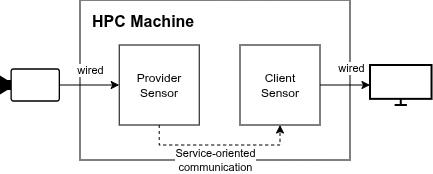
\includegraphics[width=0.75\textwidth]{Images/chap3/image_methodology/machineDesign/high_level.png}
    \vspace{0.5cm}
    \caption{High Level Architecture of Prototype Project}
    \label{fig:hla_project}
\end{figure}

Based on the defined high-level architecture, the Adaptive AUTOSAR configuration process is carried out in a stepwise manner, following the recommended methodology. The overall system design is progressively refined from an abstract architectural view to concrete deployment and execution artifacts.

First, the Machine Design and Machine Manifest are configured to define the physical execution environment of the system. This step specifies the target machine, network interfaces, service discovery settings, operating system platform modules, and lifecycle-related parameters, forming the foundation on which all applications and services are deployed.

Next, the Service Interface Design and Mapping phase focuses on defining the service-oriented communication between applications. During this stage, data types, service interfaces, service instances, and deployment configurations are specified, and abstract service definitions are bound to concrete network endpoints. This step enables standardized and loosely coupled interaction between the Provider Sensor and Client Sensor.

Finally, the Application Design phase models the adaptive applications themselves. Executables are defined and configured, ports are mapped to service interfaces, application processes are created, and startup and lifecycle behaviors are specified. Through this step, the logical application design is concretely mapped onto the target machine, completing the system configuration prior to code and manifest generation.

\subsubsection{Machine Design and Machine Manifest}

% Define Ethernet network endpoint
\begin{figure}[H]
    \centering
    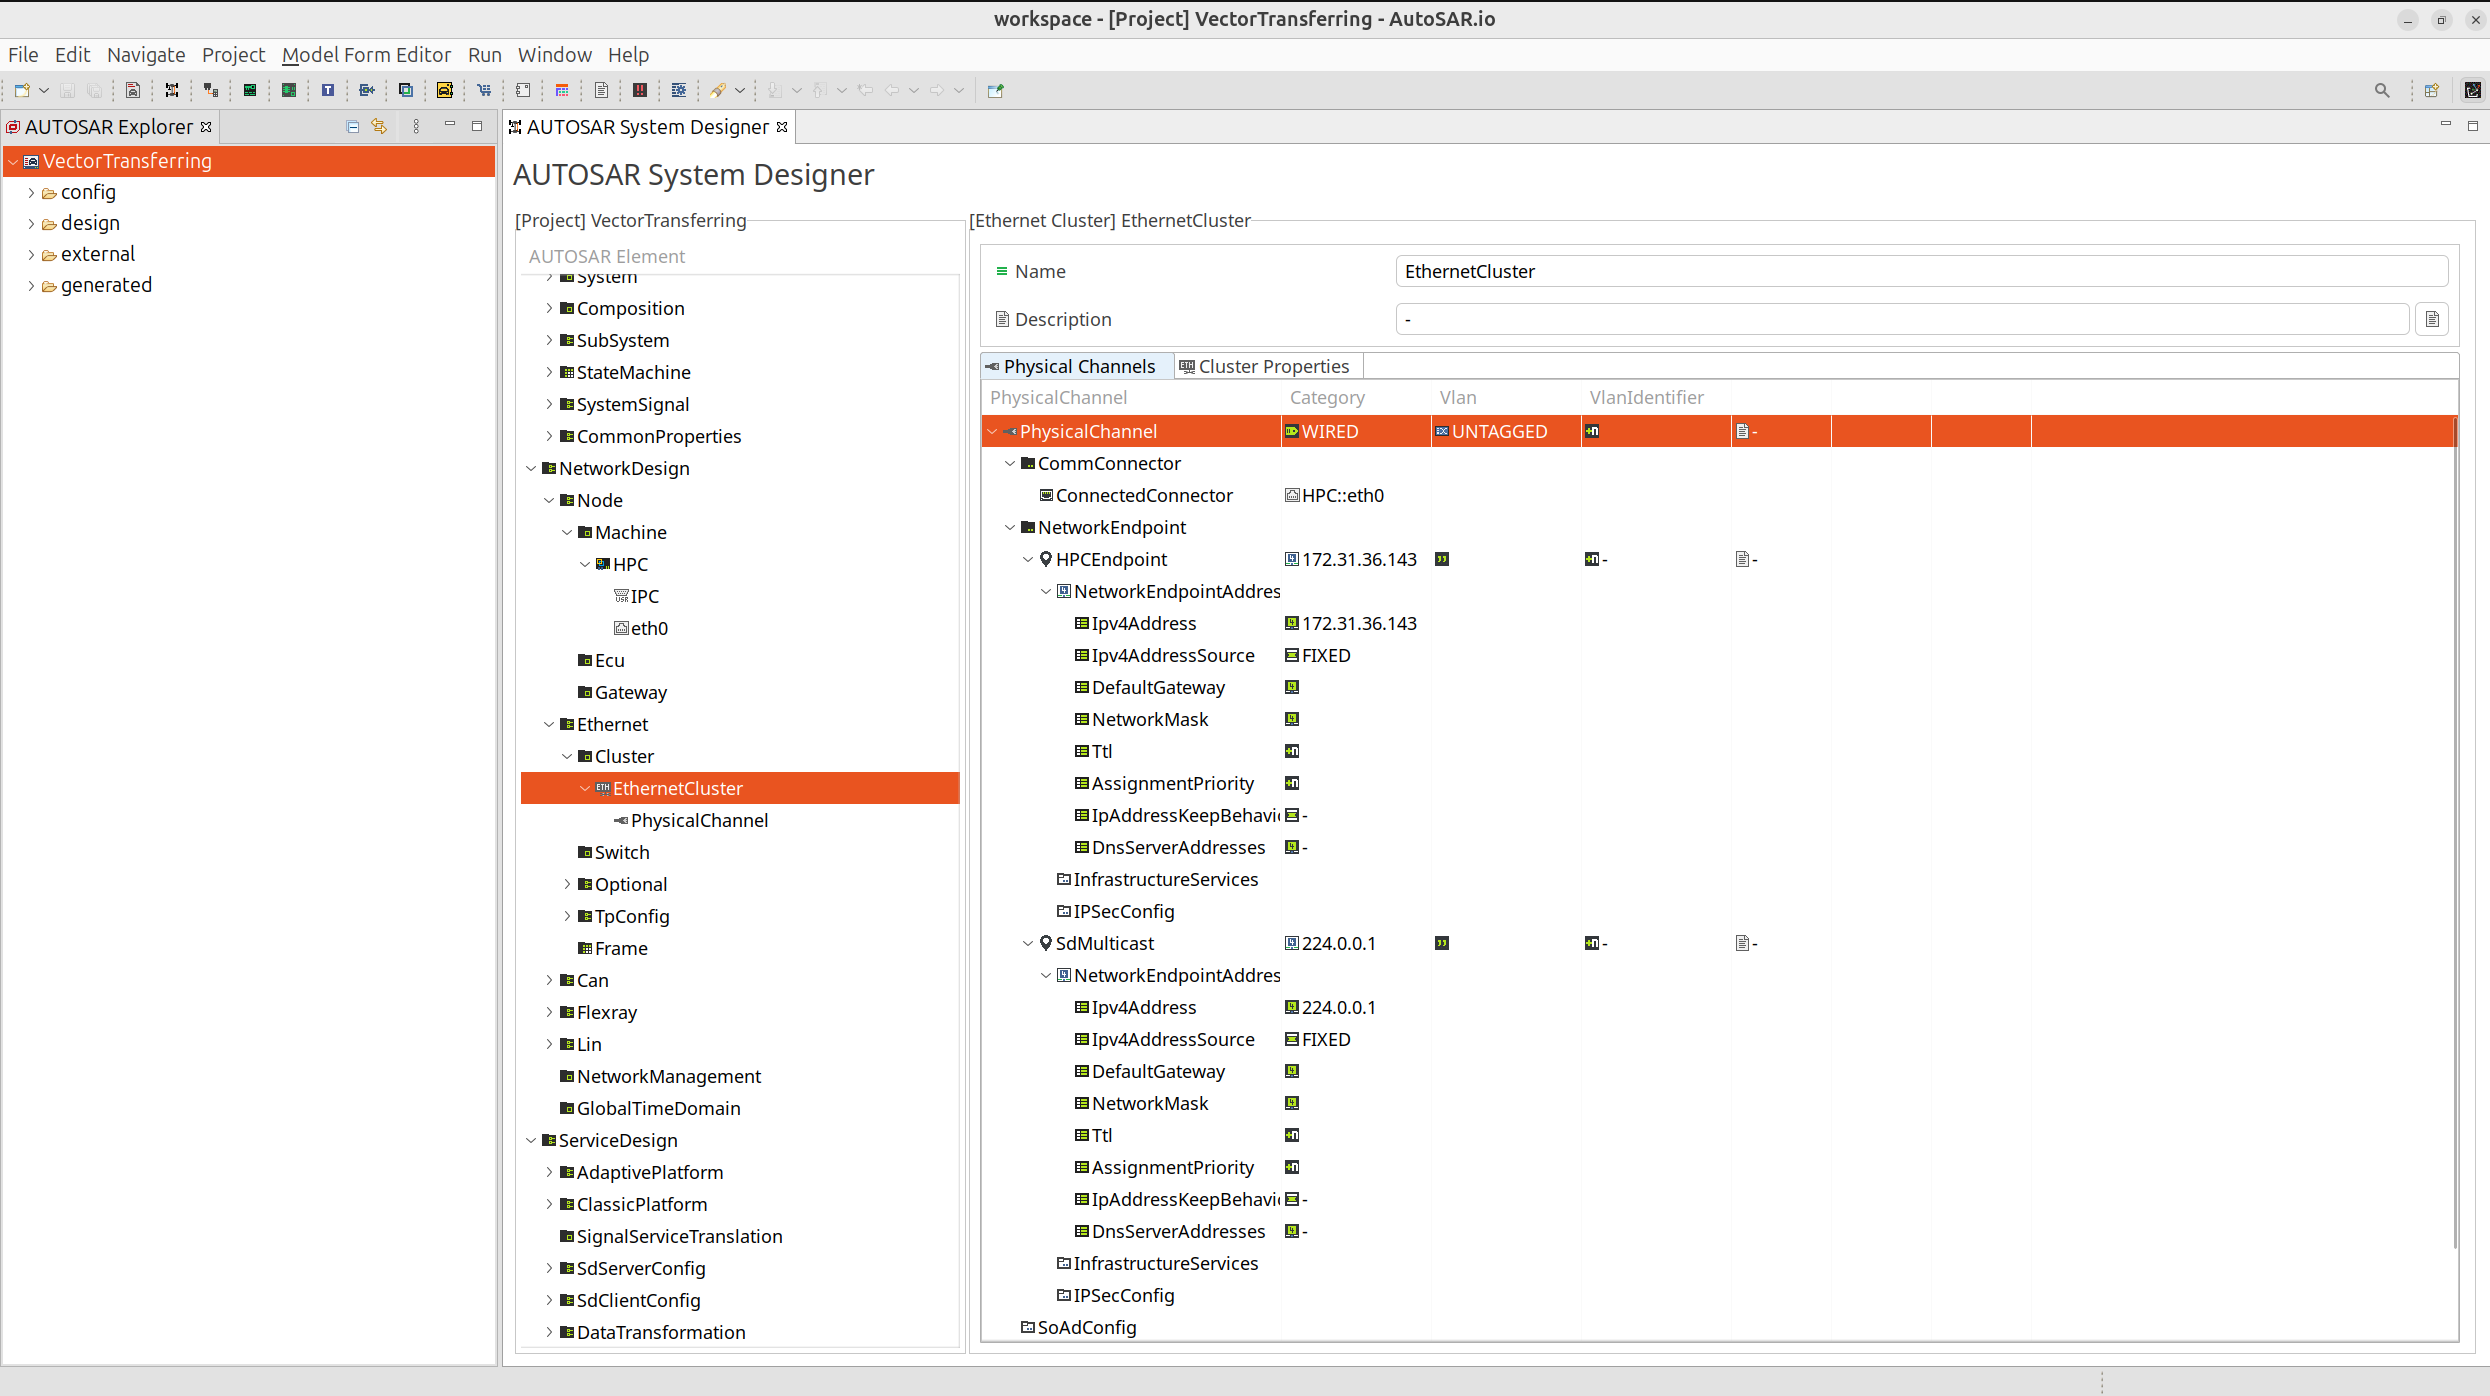
\includegraphics[width=0.75\textwidth]{Images/chap3/image_methodology/machineDesign/defineEthernet.png}
    \vspace{0.5cm}
    \caption{Definition of Ethernet Network Endpoint in Machine Design}
    \label{fig:machine_define_ethernet}
\end{figure}

Figure~\ref{fig:machine_define_ethernet} illustrates the detailed configuration of an Ethernet network endpoint within the AUTOSAR System Designer. An EthernetCluster is defined with a wired physical channel, where the VLAN mode is set to untagged, indicating that no VLAN identifier is applied to the network traffic. The machine node labeled HPC is connected to this cluster through the communication connector HPC eth0, which represents the physical Ethernet interface of the target machine.

The network endpoint configuration specifies a fixed IPv4 address of 172.31.36.143, with the address source explicitly defined as fixed to ensure deterministic network behavior. In addition to the unicast endpoint, a multicast configuration is also present using the IPv4 address 224.0.0.1, which is commonly used for service discovery communication. These settings collectively define how the machine participates in both point to point and multicast Ethernet communication, forming a stable networking foundation for Adaptive AUTOSAR service based applications.

% Add Ethernet configuration to Machine Design
\begin{figure}[H]
    \centering
    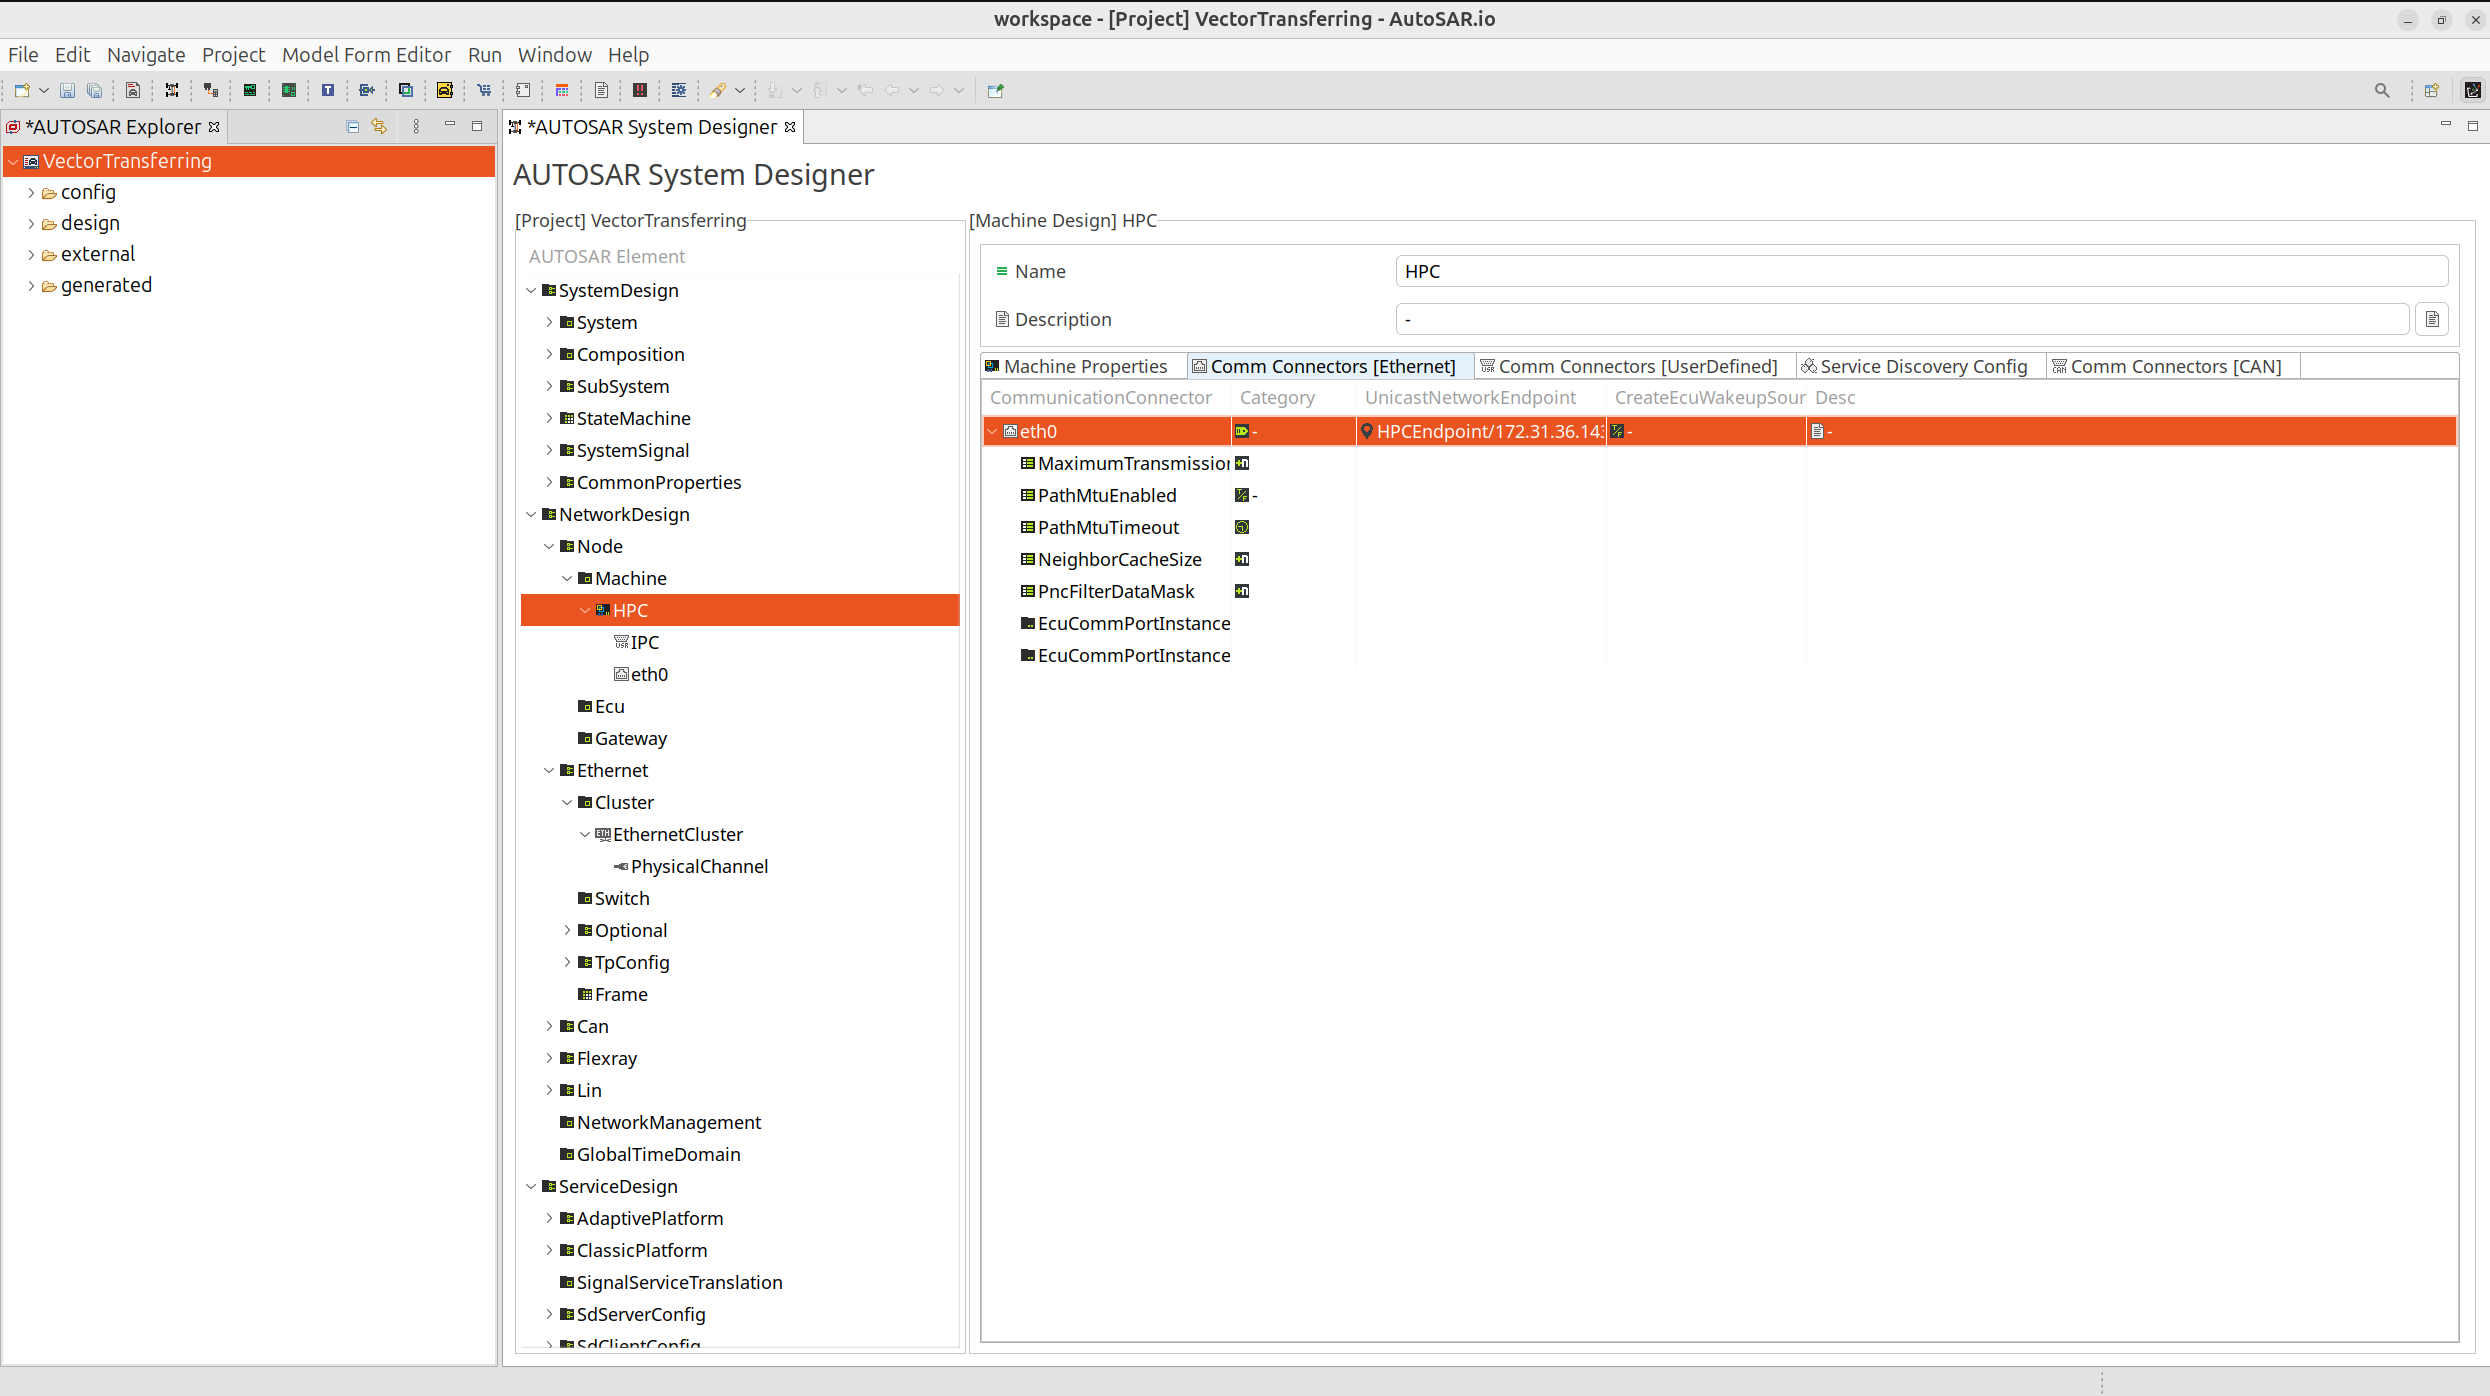
\includegraphics[width=0.75\textwidth]{Images/chap3/image_methodology/machineDesign/addEthMachineDesign.png}
    \vspace{0.5cm}
    \caption{Integration of Ethernet Configuration into Machine Design}
    \label{fig:machine_add_eth_design}
\end{figure}

Figure~\ref{fig:machine_add_eth_design} depicts how the HPC machine is linked to its network interface through the eth0 connector in the Machine Design view. This connector is mapped to a unicast endpoint identified as HPCEndpoint with the IPv4 address 172.31.36.143, defining the machine’s network presence within the Adaptive AUTOSAR system. The figure also highlights adjustable communication parameters such as transmission limits and path MTU handling, which allow the network behavior to be adapted while maintaining reliable data exchange at runtime.

% Configure Service Discovery in Machine Design
\begin{figure}[H]
    \centering
    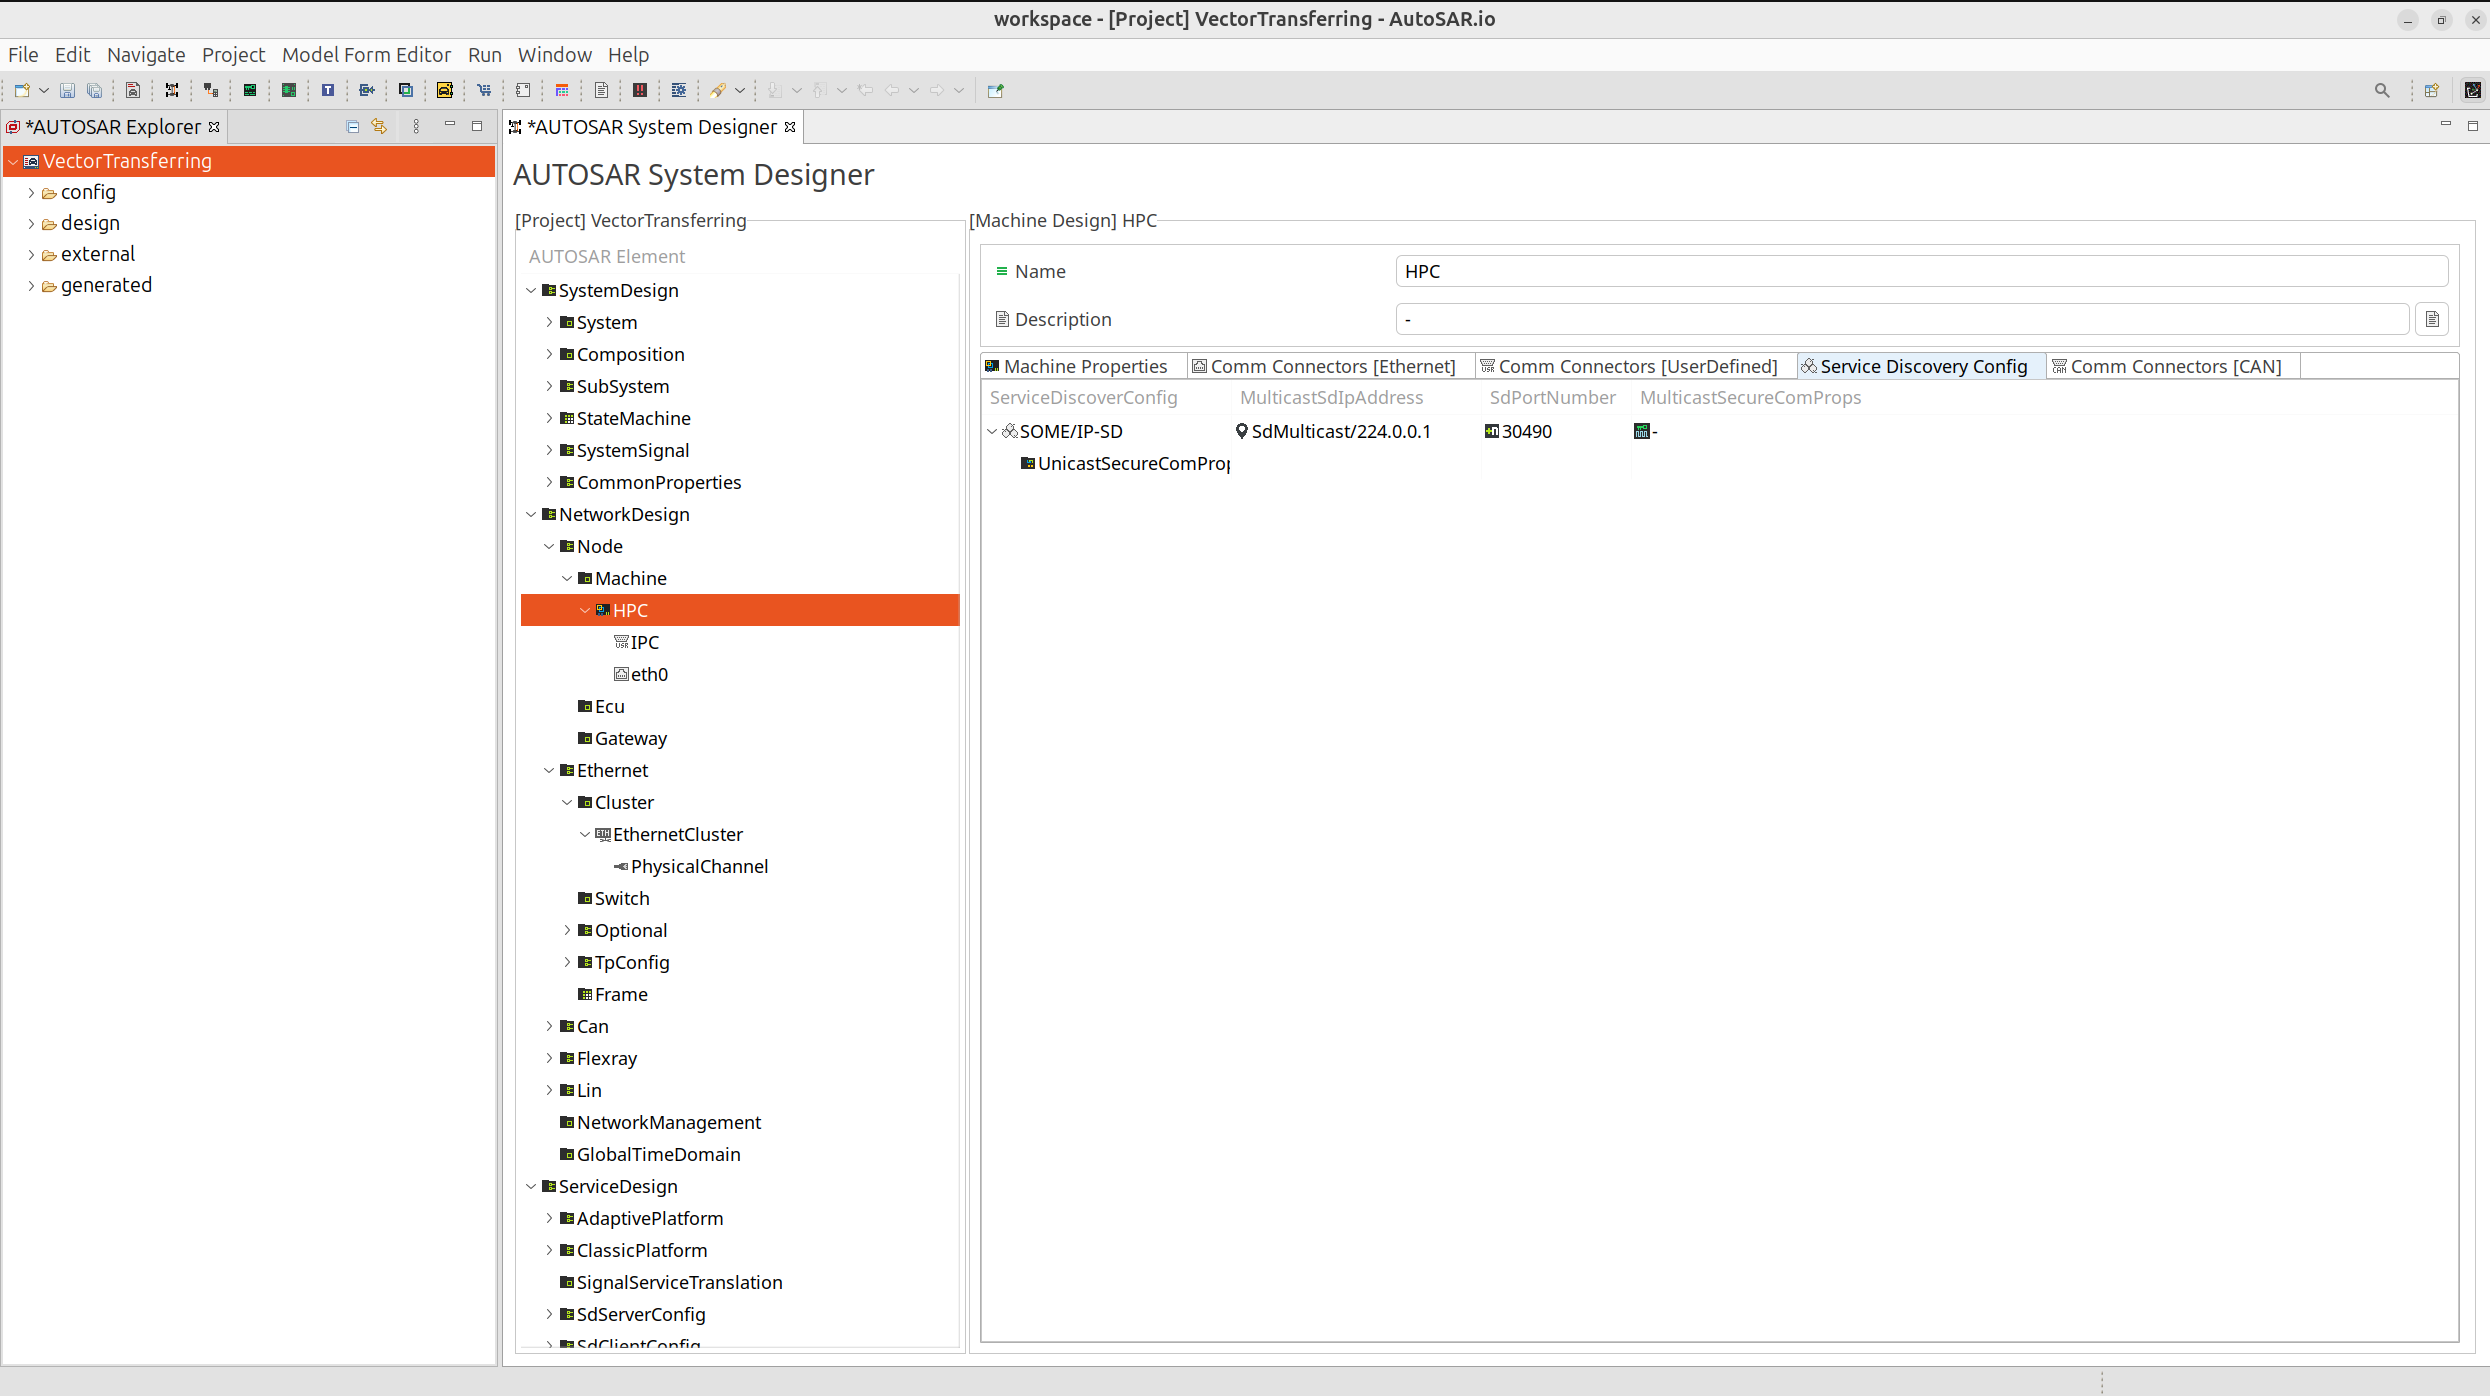
\includegraphics[width=0.75\textwidth]{Images/chap3/image_methodology/machineDesign/addSdConfigMachineDesign.png}
    \vspace{0.5cm}
    \caption{Service Discovery Configuration in Machine Design}
    \label{fig:machine_sd_config}
\end{figure}

Figure~\ref{fig:machine_sd_config} illustrates the Service Discovery setup for the HPC machine within the Machine Design environment. The SOME IP Service Discovery mechanism is configured using the multicast address 224.0.0.1 together with the service discovery port number 30490, which enables applications to announce and detect available services at runtime. This configuration allows dynamic interaction between Adaptive AUTOSAR applications while supporting flexible service availability without relying on static communication bindings.

% Configure Diagnostic Log and Trace (DLT)
\begin{figure}[H]
    \centering
    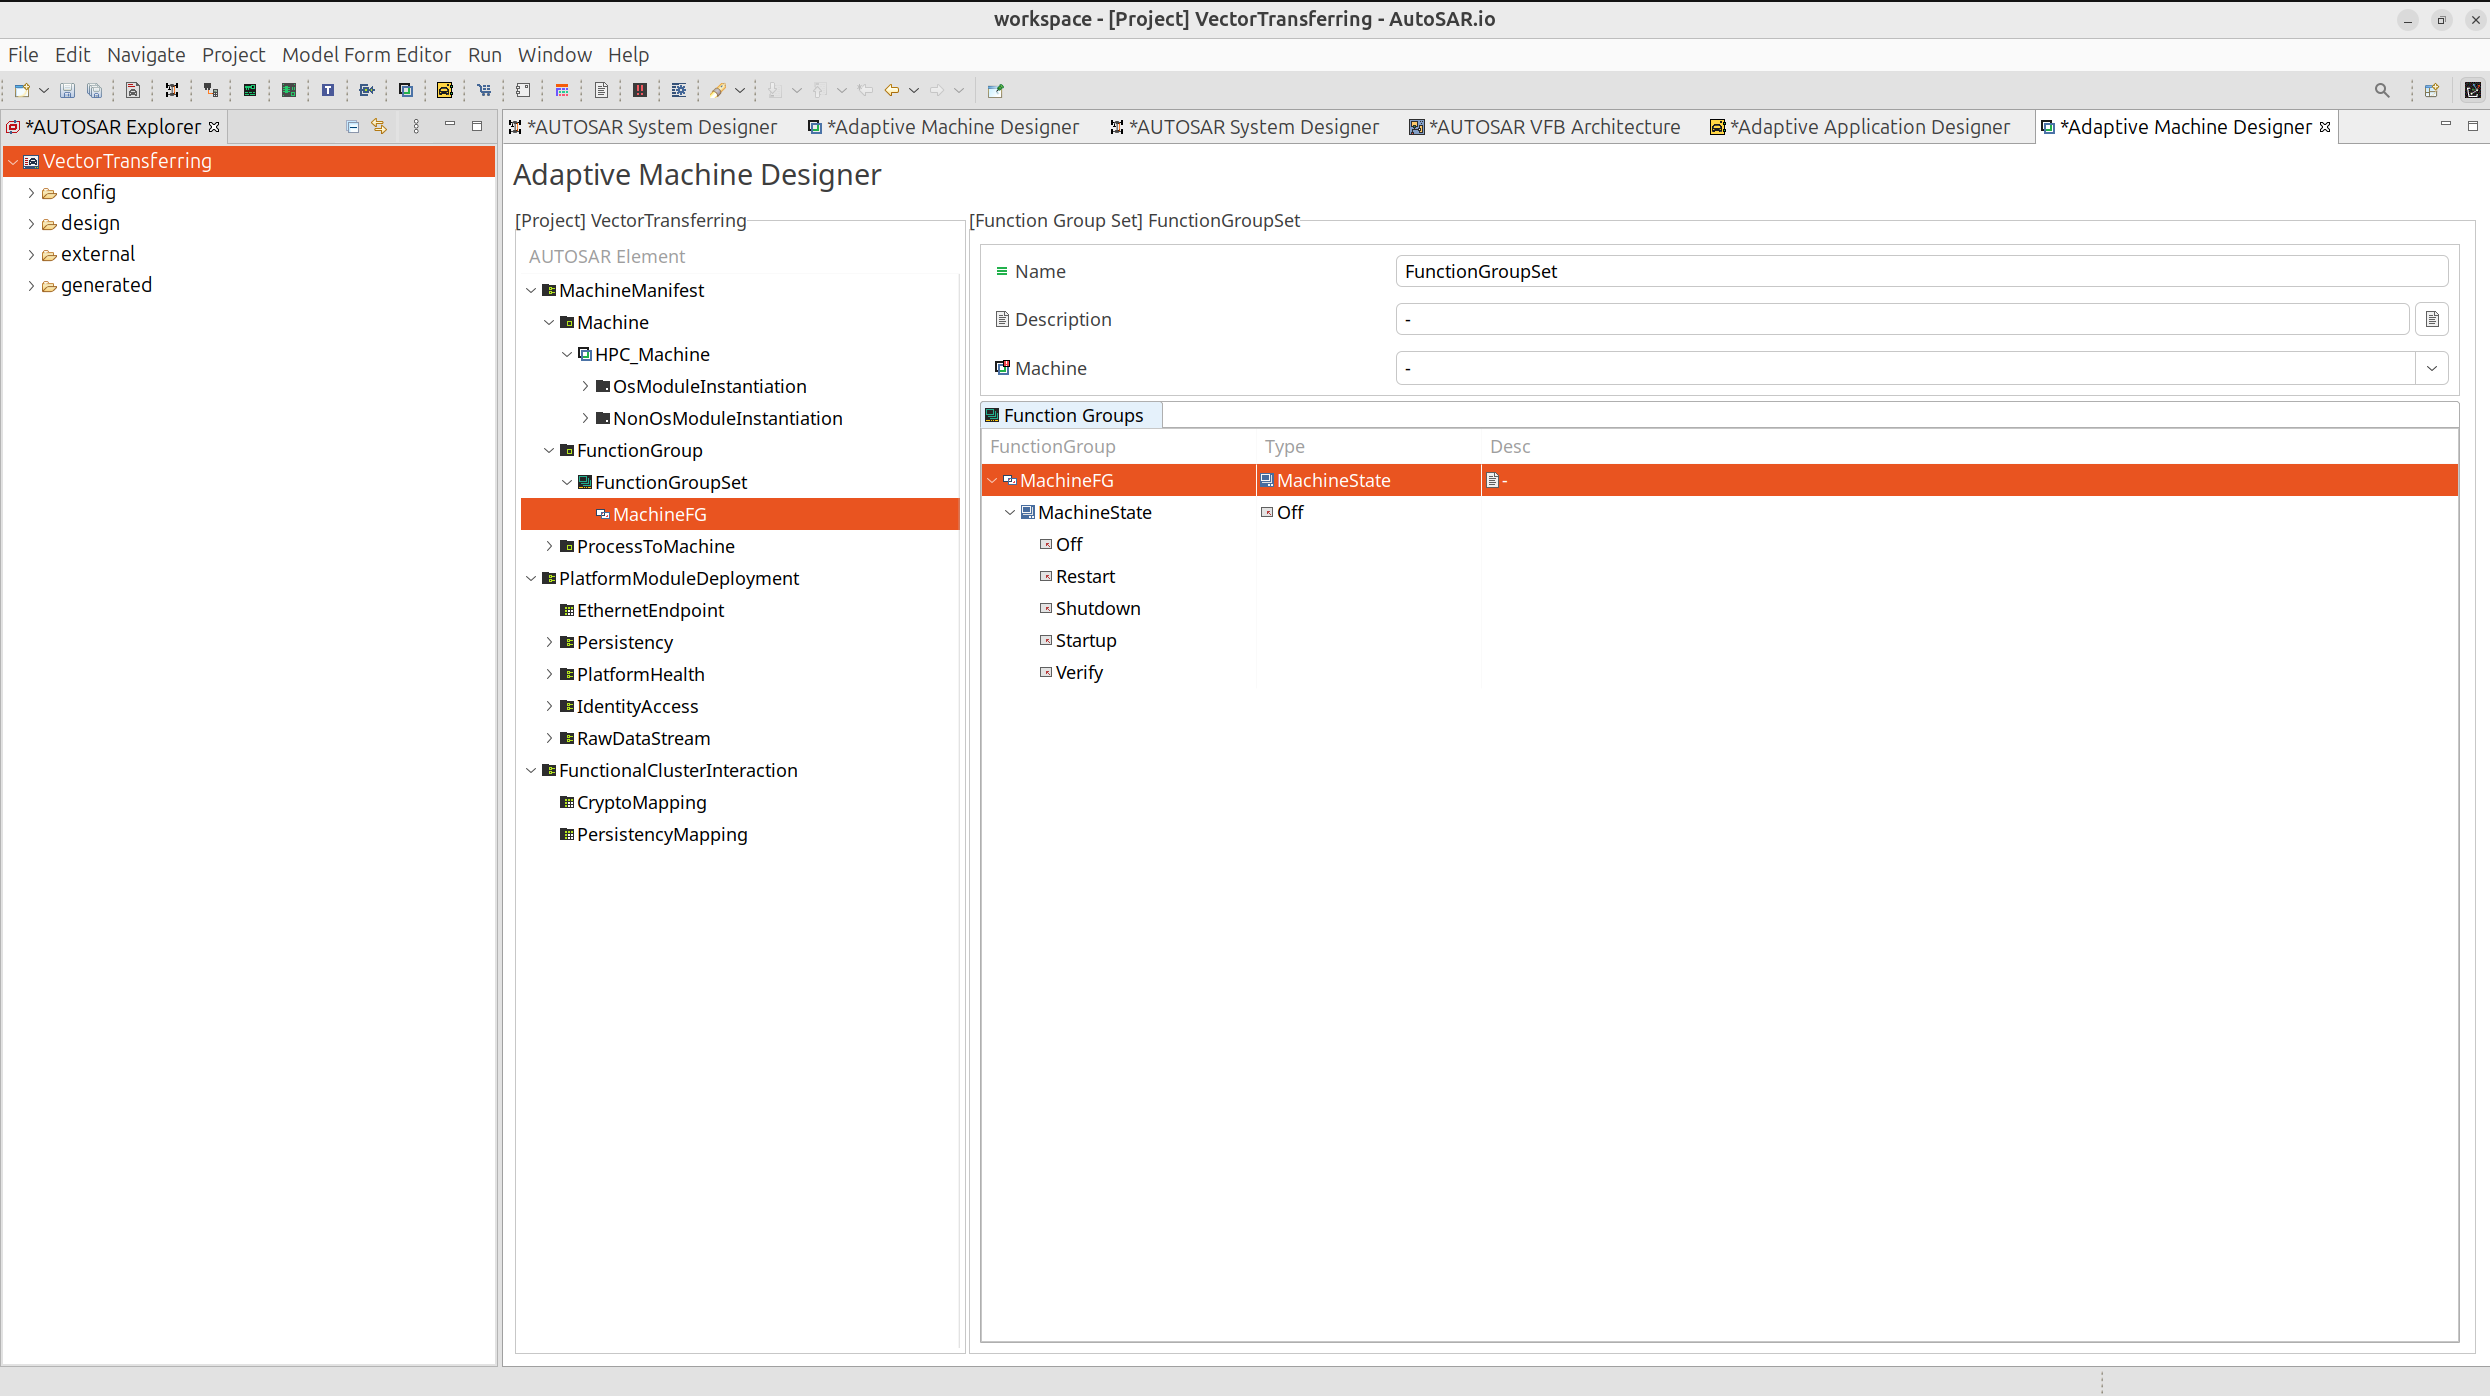
\includegraphics[width=0.75\textwidth]{Images/chap3/image_methodology/machineDesign/configMachineFG.png}
    \vspace{0.5cm}
    \caption{Machine Function Group States Configuration}
    \label{fig:machine_fg_config}
\end{figure}

The figure \ref{fig:machine_fg_config} presents the configuration of the machine function group for the HPC\_Machine in the Adaptive Machine Designer. A function group named MachineFG is defined with the MachineState type, which includes states such as Off, Startup, Verify, Restart, and Shutdown. This configuration governs how the machine progresses through its operational lifecycle, ensuring that platform services and applications are activated and controlled according to well defined system states during runtime execution.

% Final Machine Manifest
\begin{figure}[H]
    \centering
    
\includegraphics[width=0.75\textwidth]{Images/chap3/image_methodology/machineDesign/machineManifest.png}
    \vspace{0.5cm}
    \caption{Machine Manifest for Adaptive AUTOSAR Deployment}
    \label{fig:machine_manifest}
\end{figure}

The figure \ref{fig:machine_manifest} presents the Machine Manifest of the HPC\_Machine as defined in the Adaptive Machine Designer. This manifest consolidates all machine level configurations by referencing the previously defined Machine Design, including the SOME/IP Service Discovery endpoint with the multicast address 224.0.0.1 and port 30490, as well as the Ethernet connector bound to the eth0 interface. In addition, user defined connectors and inter process communication settings are integrated, forming a complete description of the communication capabilities of the target machine.

Furthermore, the manifest specifies essential execution and platform related properties such as trusted platform execution mode, default application timeout, and processor configuration. The processor section defines the available CPU resources and core assignment, while function group and process to machine mappings establish how applications are bound to machine states at runtime. By combining communication, execution, and lifecycle information into a single artifact, the Machine Manifest serves as the final deployment blueprint for Adaptive AUTOSAR applications.

% Configure Operating System platform module
\begin{figure}[H]
    \centering
    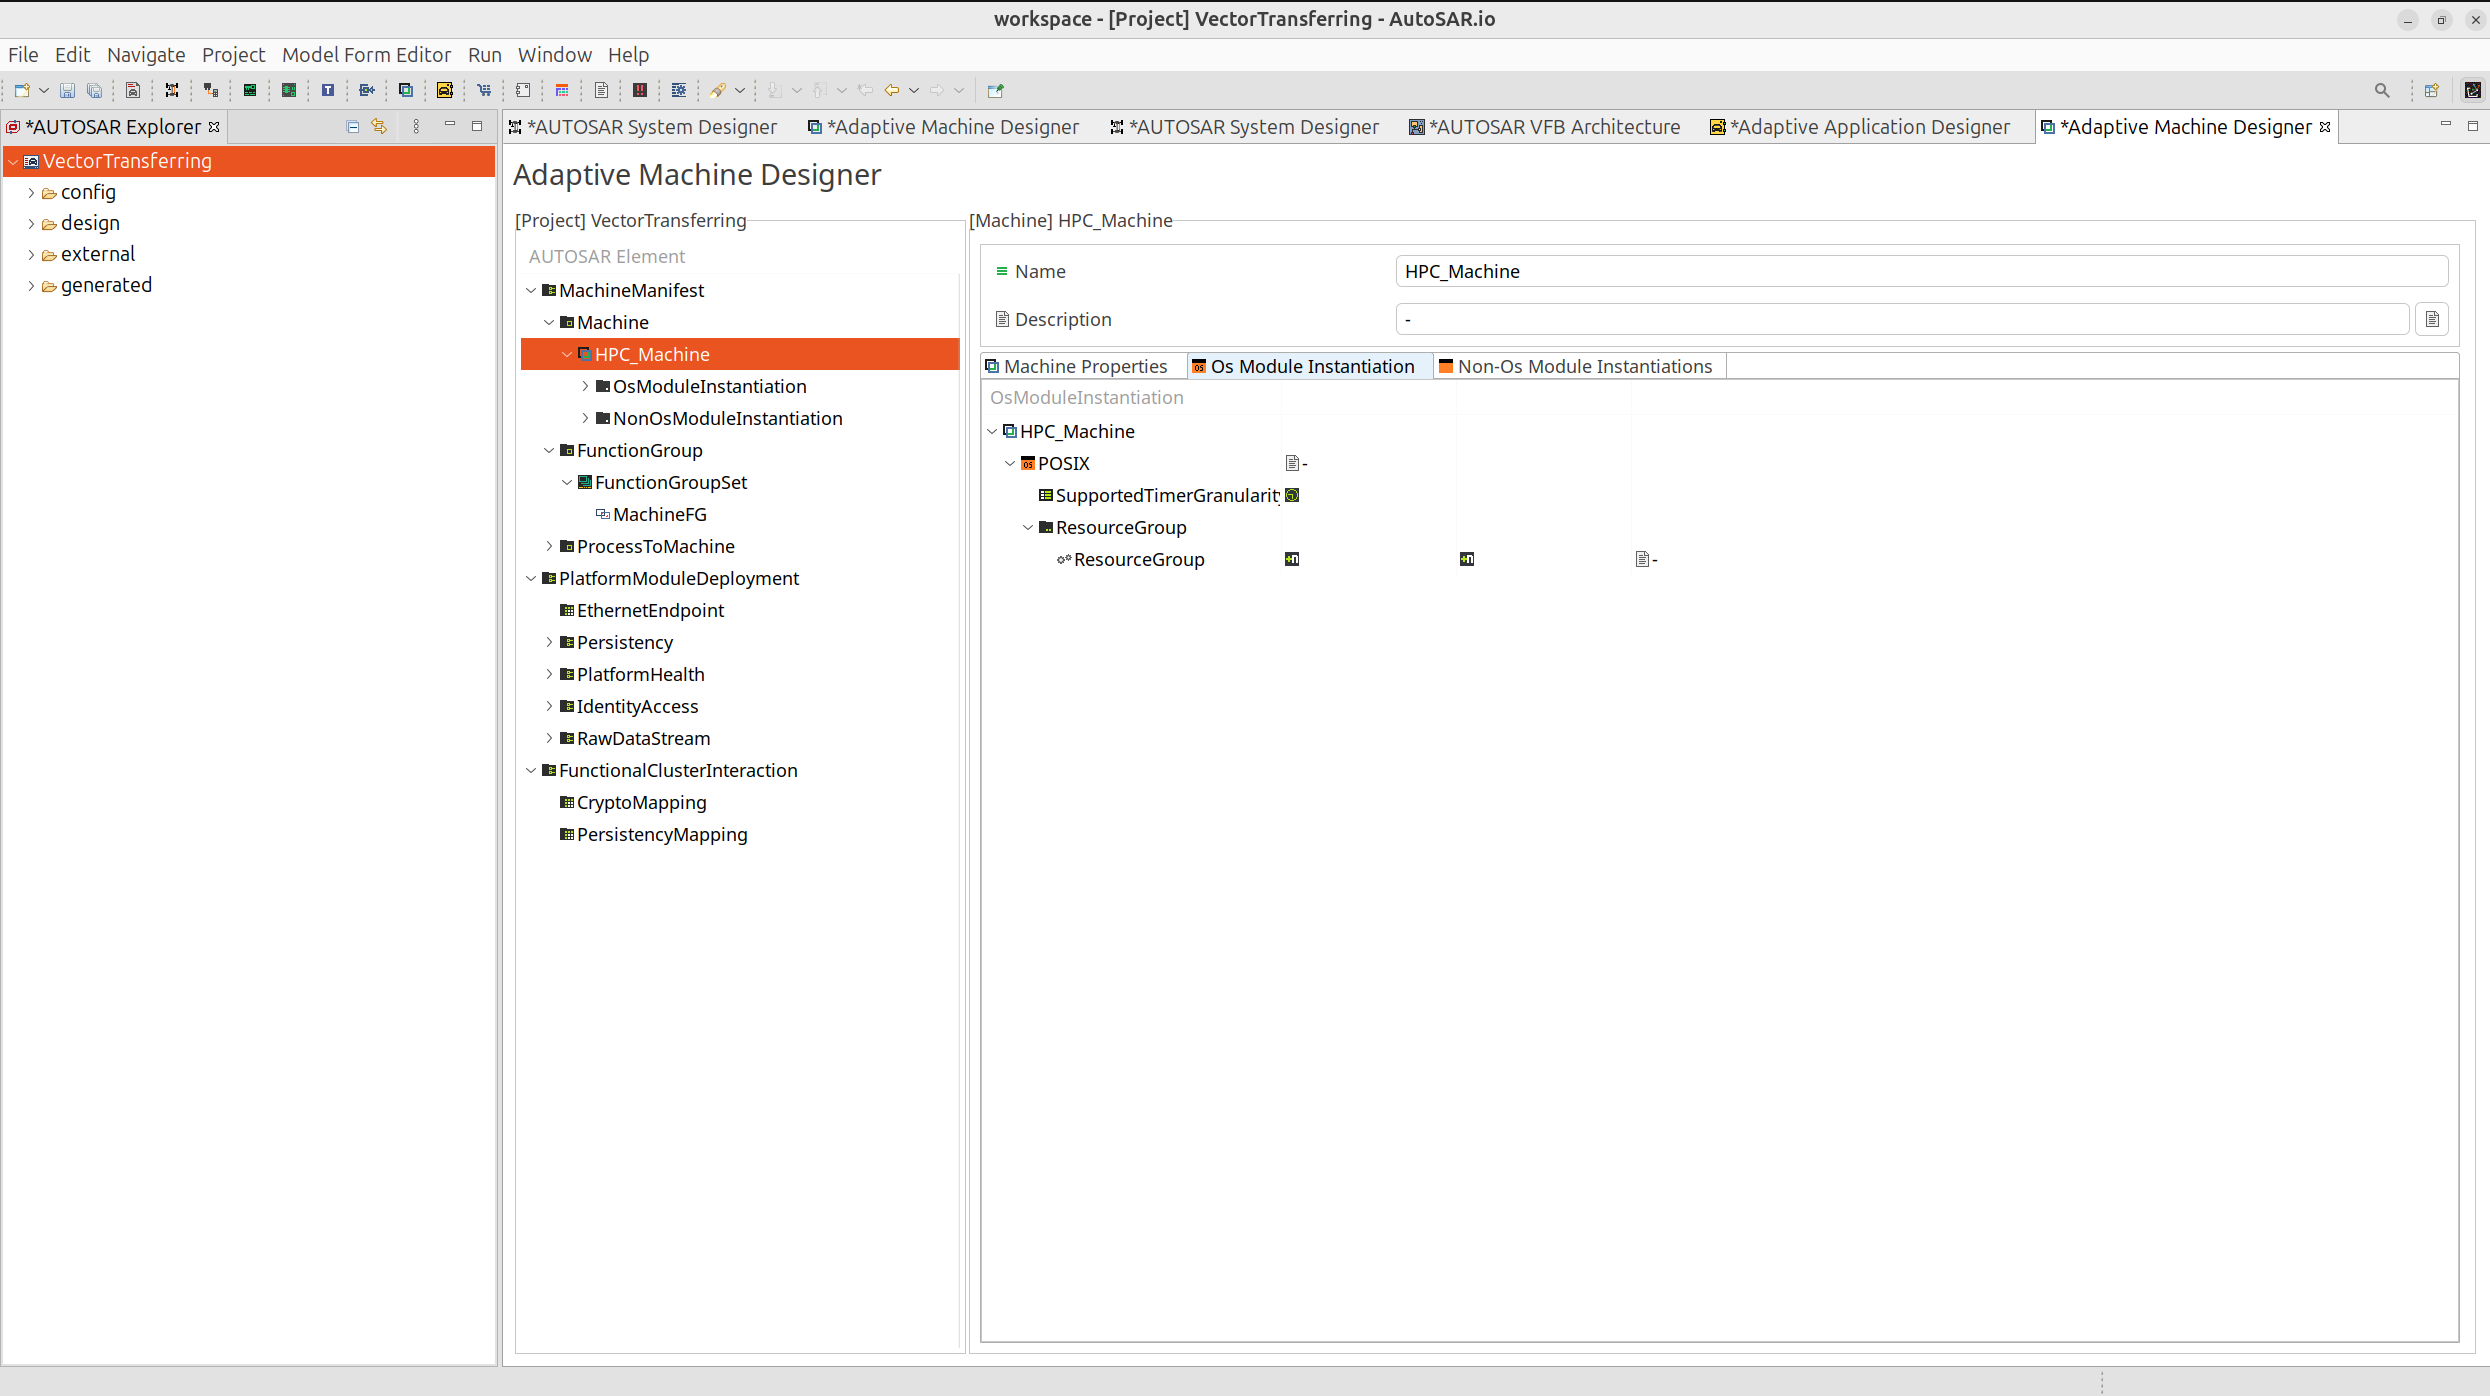
\includegraphics[width=0.75\textwidth]{Images/chap3/image_methodology/machineDesign/configOSModule.png}
    \vspace{0.5cm}
    \caption{Operating System Platform Module Configuration}
    \label{fig:machine_os_module}
\end{figure}

Figure~\ref{fig:machine_os_module} shows the operating system platform module configuration for the target machine named HPC\_Machine in the Adaptive Machine Designer. The POSIX based operating system module is instantiated to define the execution environment for Adaptive AUTOSAR applications, including supported timer granularity and resource group settings. This configuration establishes the fundamental runtime services required for process scheduling and resource management on the target machine.

% Configure non-OS platform modules
\begin{figure}[H]
    \centering
    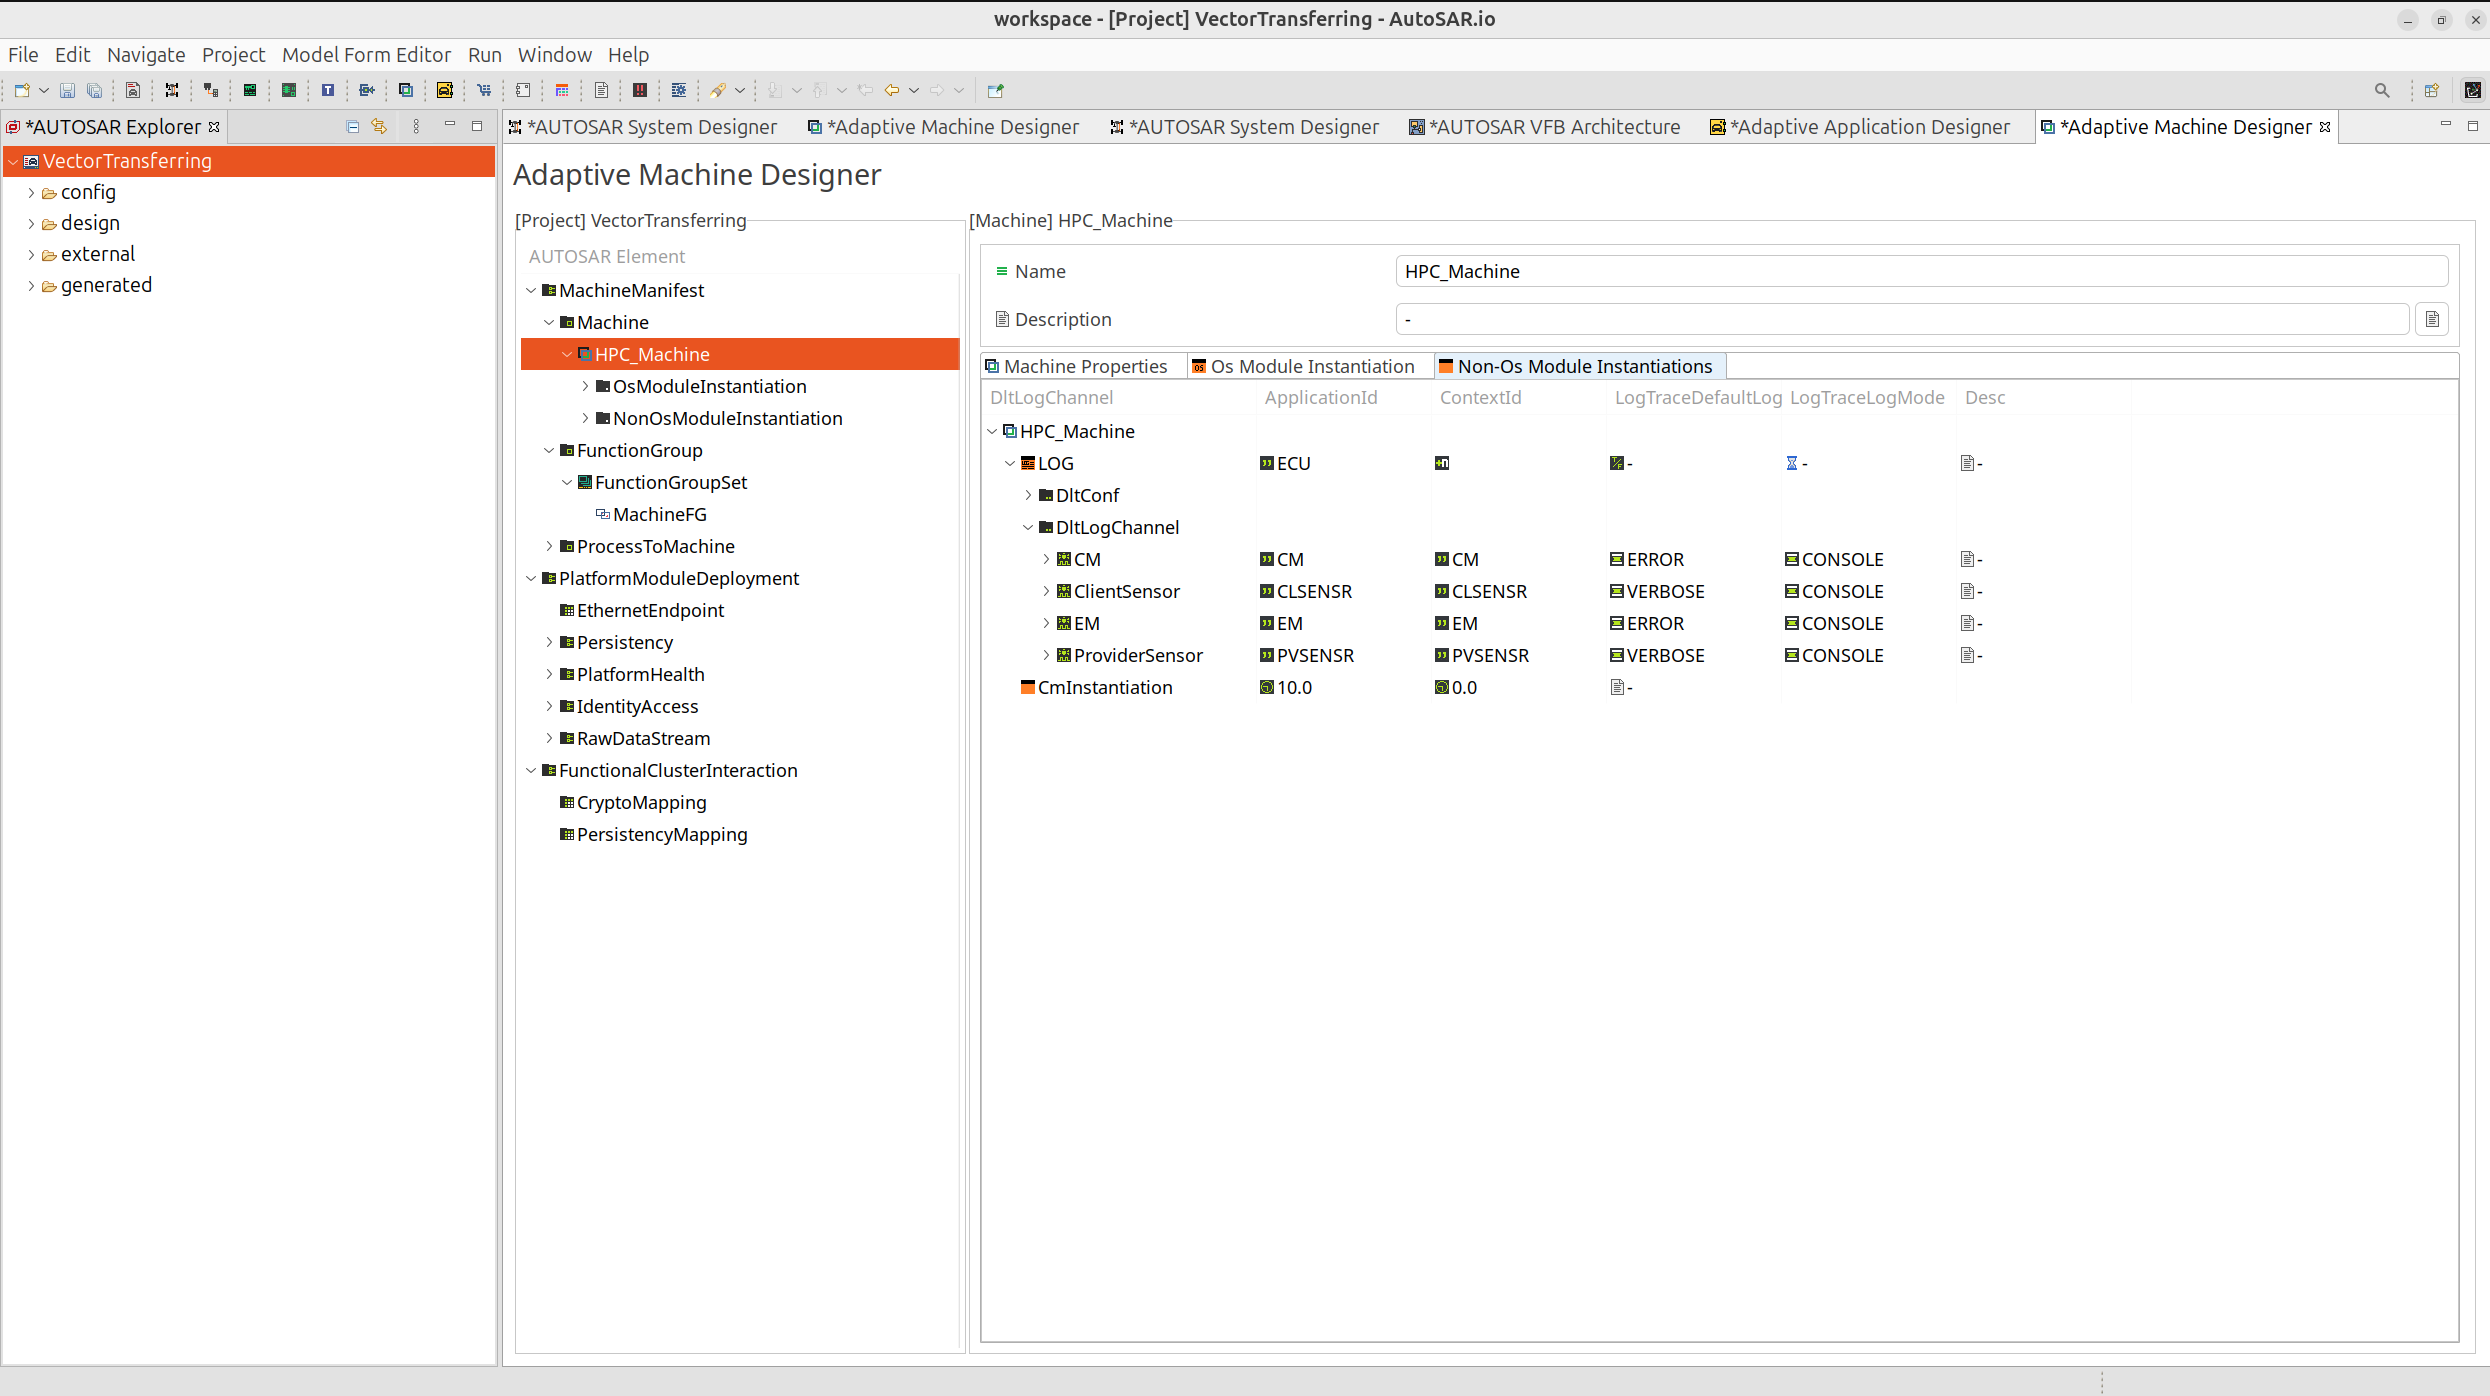
\includegraphics[width=0.75\textwidth]{Images/chap3/image_methodology/machineDesign/configNonOS.png}
    \vspace{0.5cm}
    \caption{Configuration of Non-OS Platform Modules}
    \label{fig:machine_non_os_module}
\end{figure}

Figure~\ref{fig:machine_non_os_module} presents the configuration of Diagnostic Log and Trace for the HPC\_Machine in the Adaptive Machine Designer. Several log channels are defined for different software entities, including ECU, ClientSensor, EM, and ProviderSensor, each mapped to a distinct ApplicationId and ContextId. Log levels such as ERROR and VERBOSE are specified, and the output is directed to the console, allowing developers to monitor application execution and diagnose runtime behavior.

In addition, the configuration highlights the role of CMInstantiation, which represents the Communication Management daemon responsible for inter process communication on the Adaptive Platform. This daemon enables different processes to exchange messages and supports the transport of diagnostic data between applications and platform services. By instantiating the communication manager at the machine level, the system ensures that logging, tracing, and service communication operate coherently across all running processes.

\subsubsection{Service Interface Design and Mapping}

% Define data types for service interfaces
\begin{figure}[H]
    \centering
    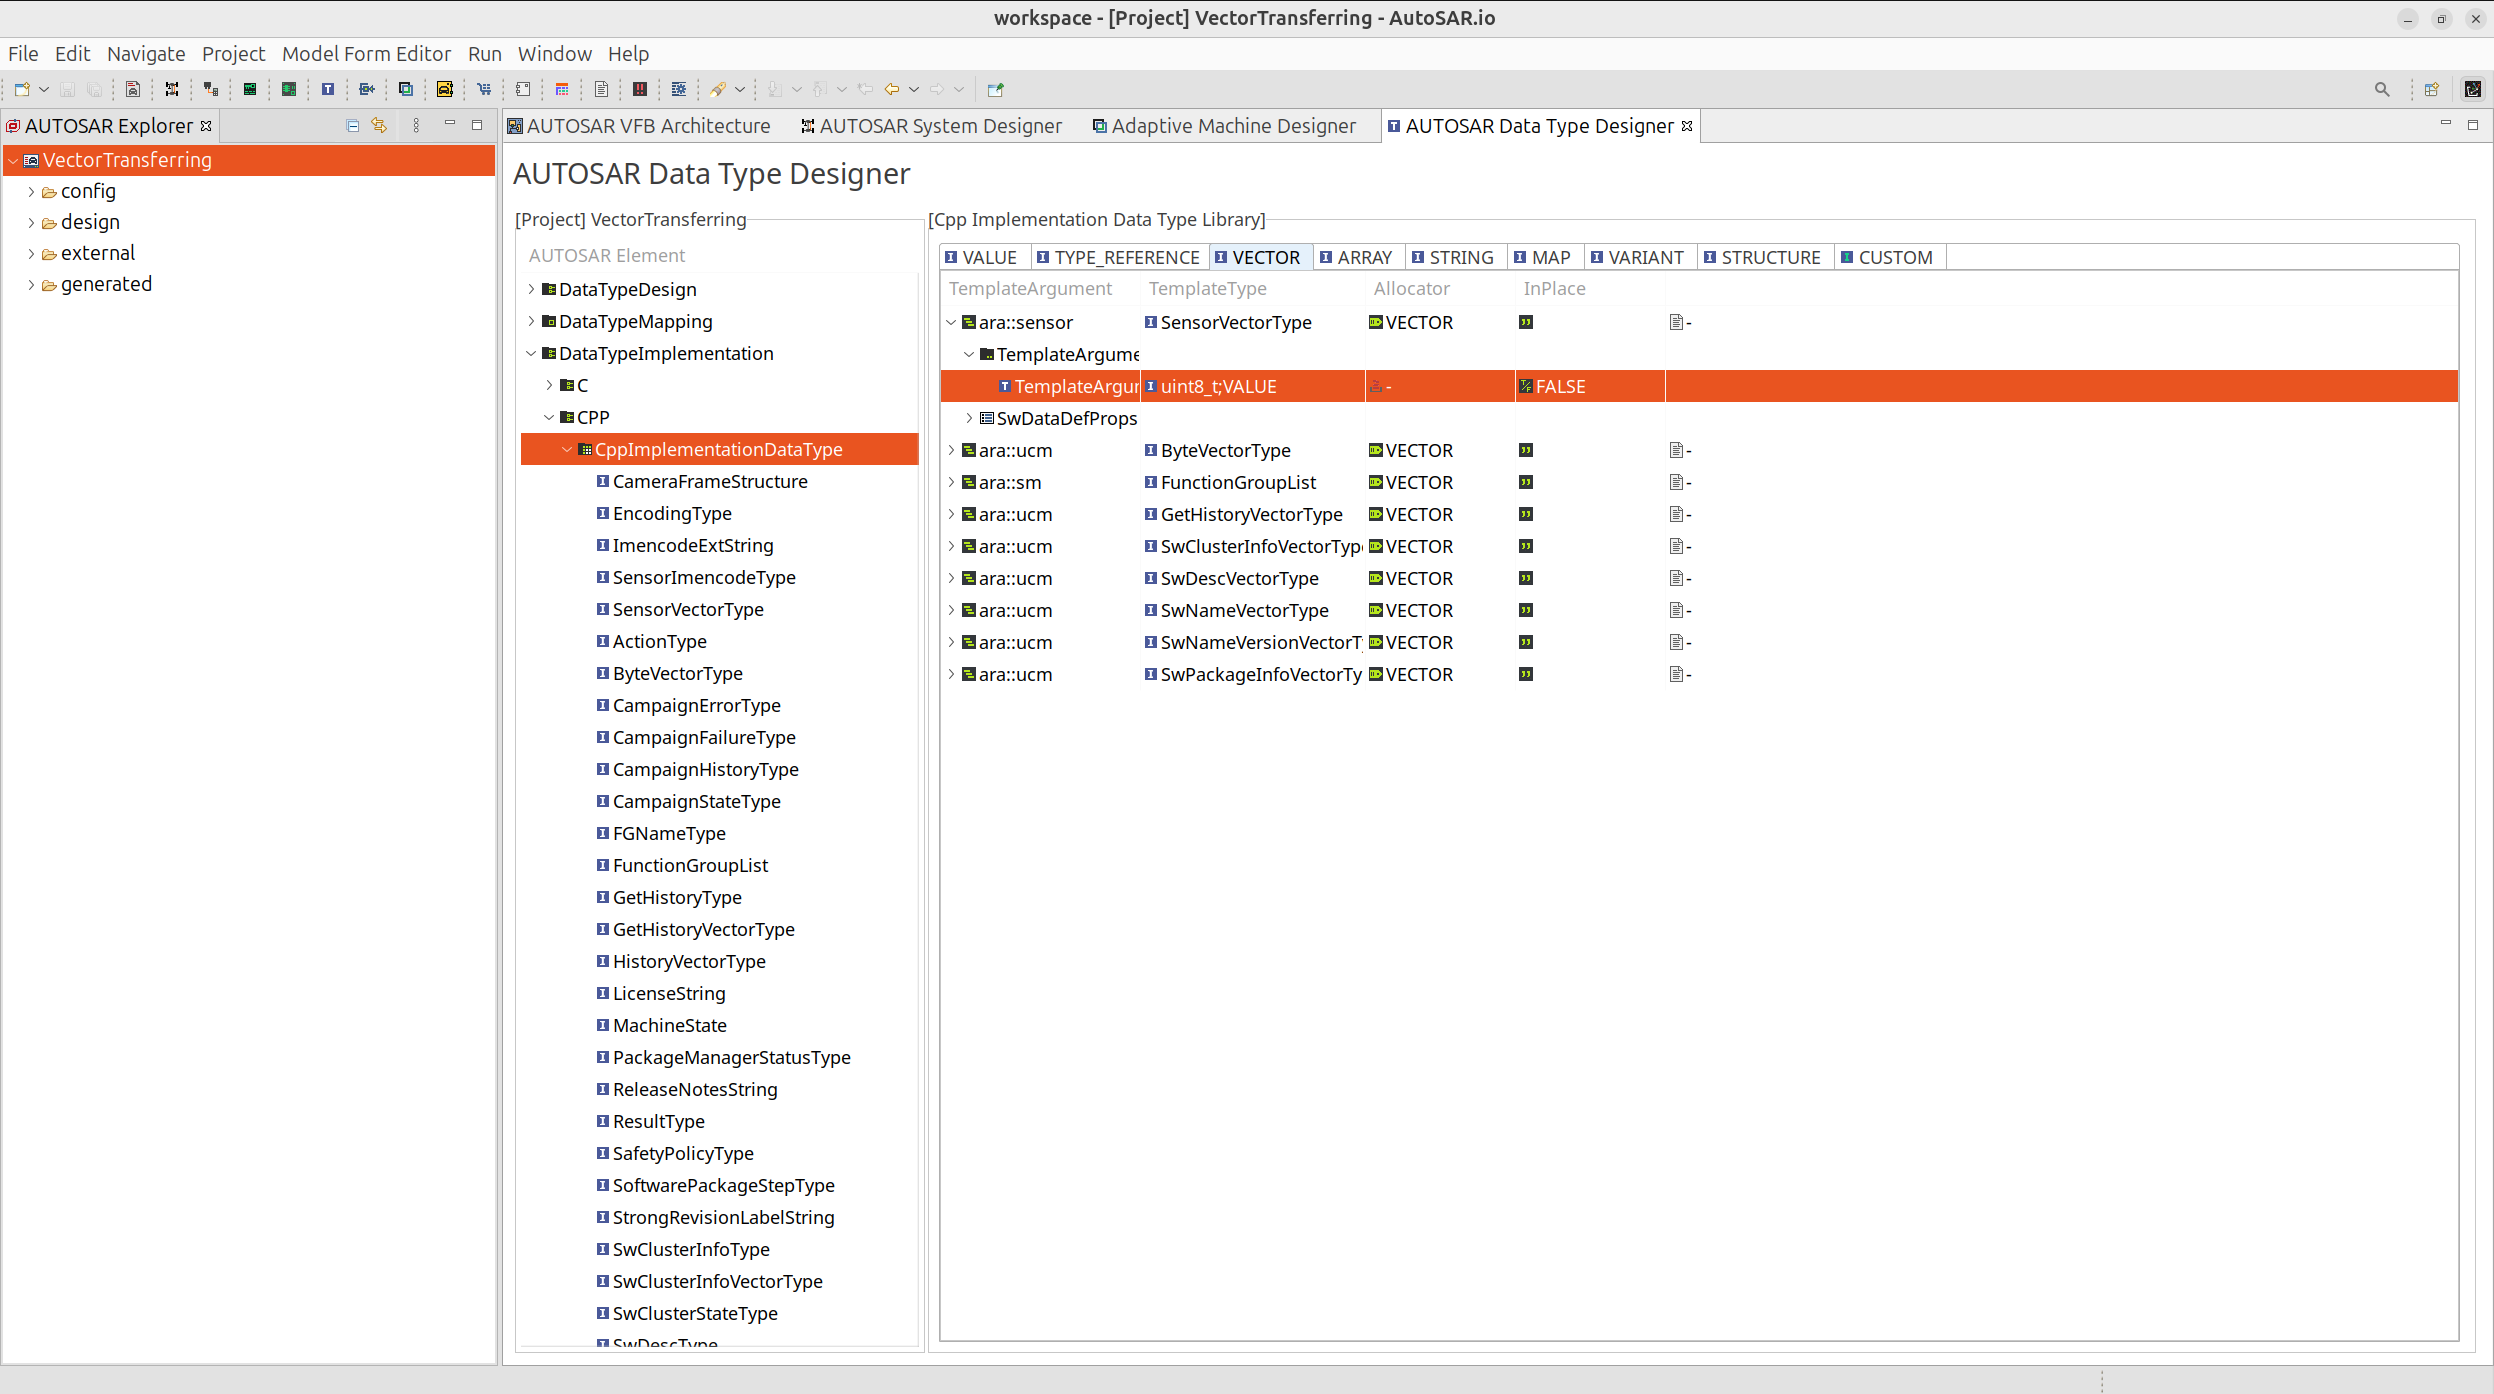
\includegraphics[width=0.75\textwidth]{Images/chap3/image_methodology/serviceInterfaceDesign/dataType.png}
    \vspace{0.5cm}
    \caption{Definition of Data Types for Service Interfaces}
    \label{fig:service_datatype}
\end{figure}

The figure~\ref{fig:service_datatype} shows the specification of C++ data types used to support service interfaces in the Adaptive AUTOSAR environment. Several vector based types are defined using template arguments, where primitive elements such as \texttt{uint8\_t} are combined to represent structured service data. These type definitions provide a clear and reusable foundation for data exchange between service providers and consumers, ensuring consistency and type safety during service oriented communication.

% Define service interface
\begin{figure}[H]
    \centering
    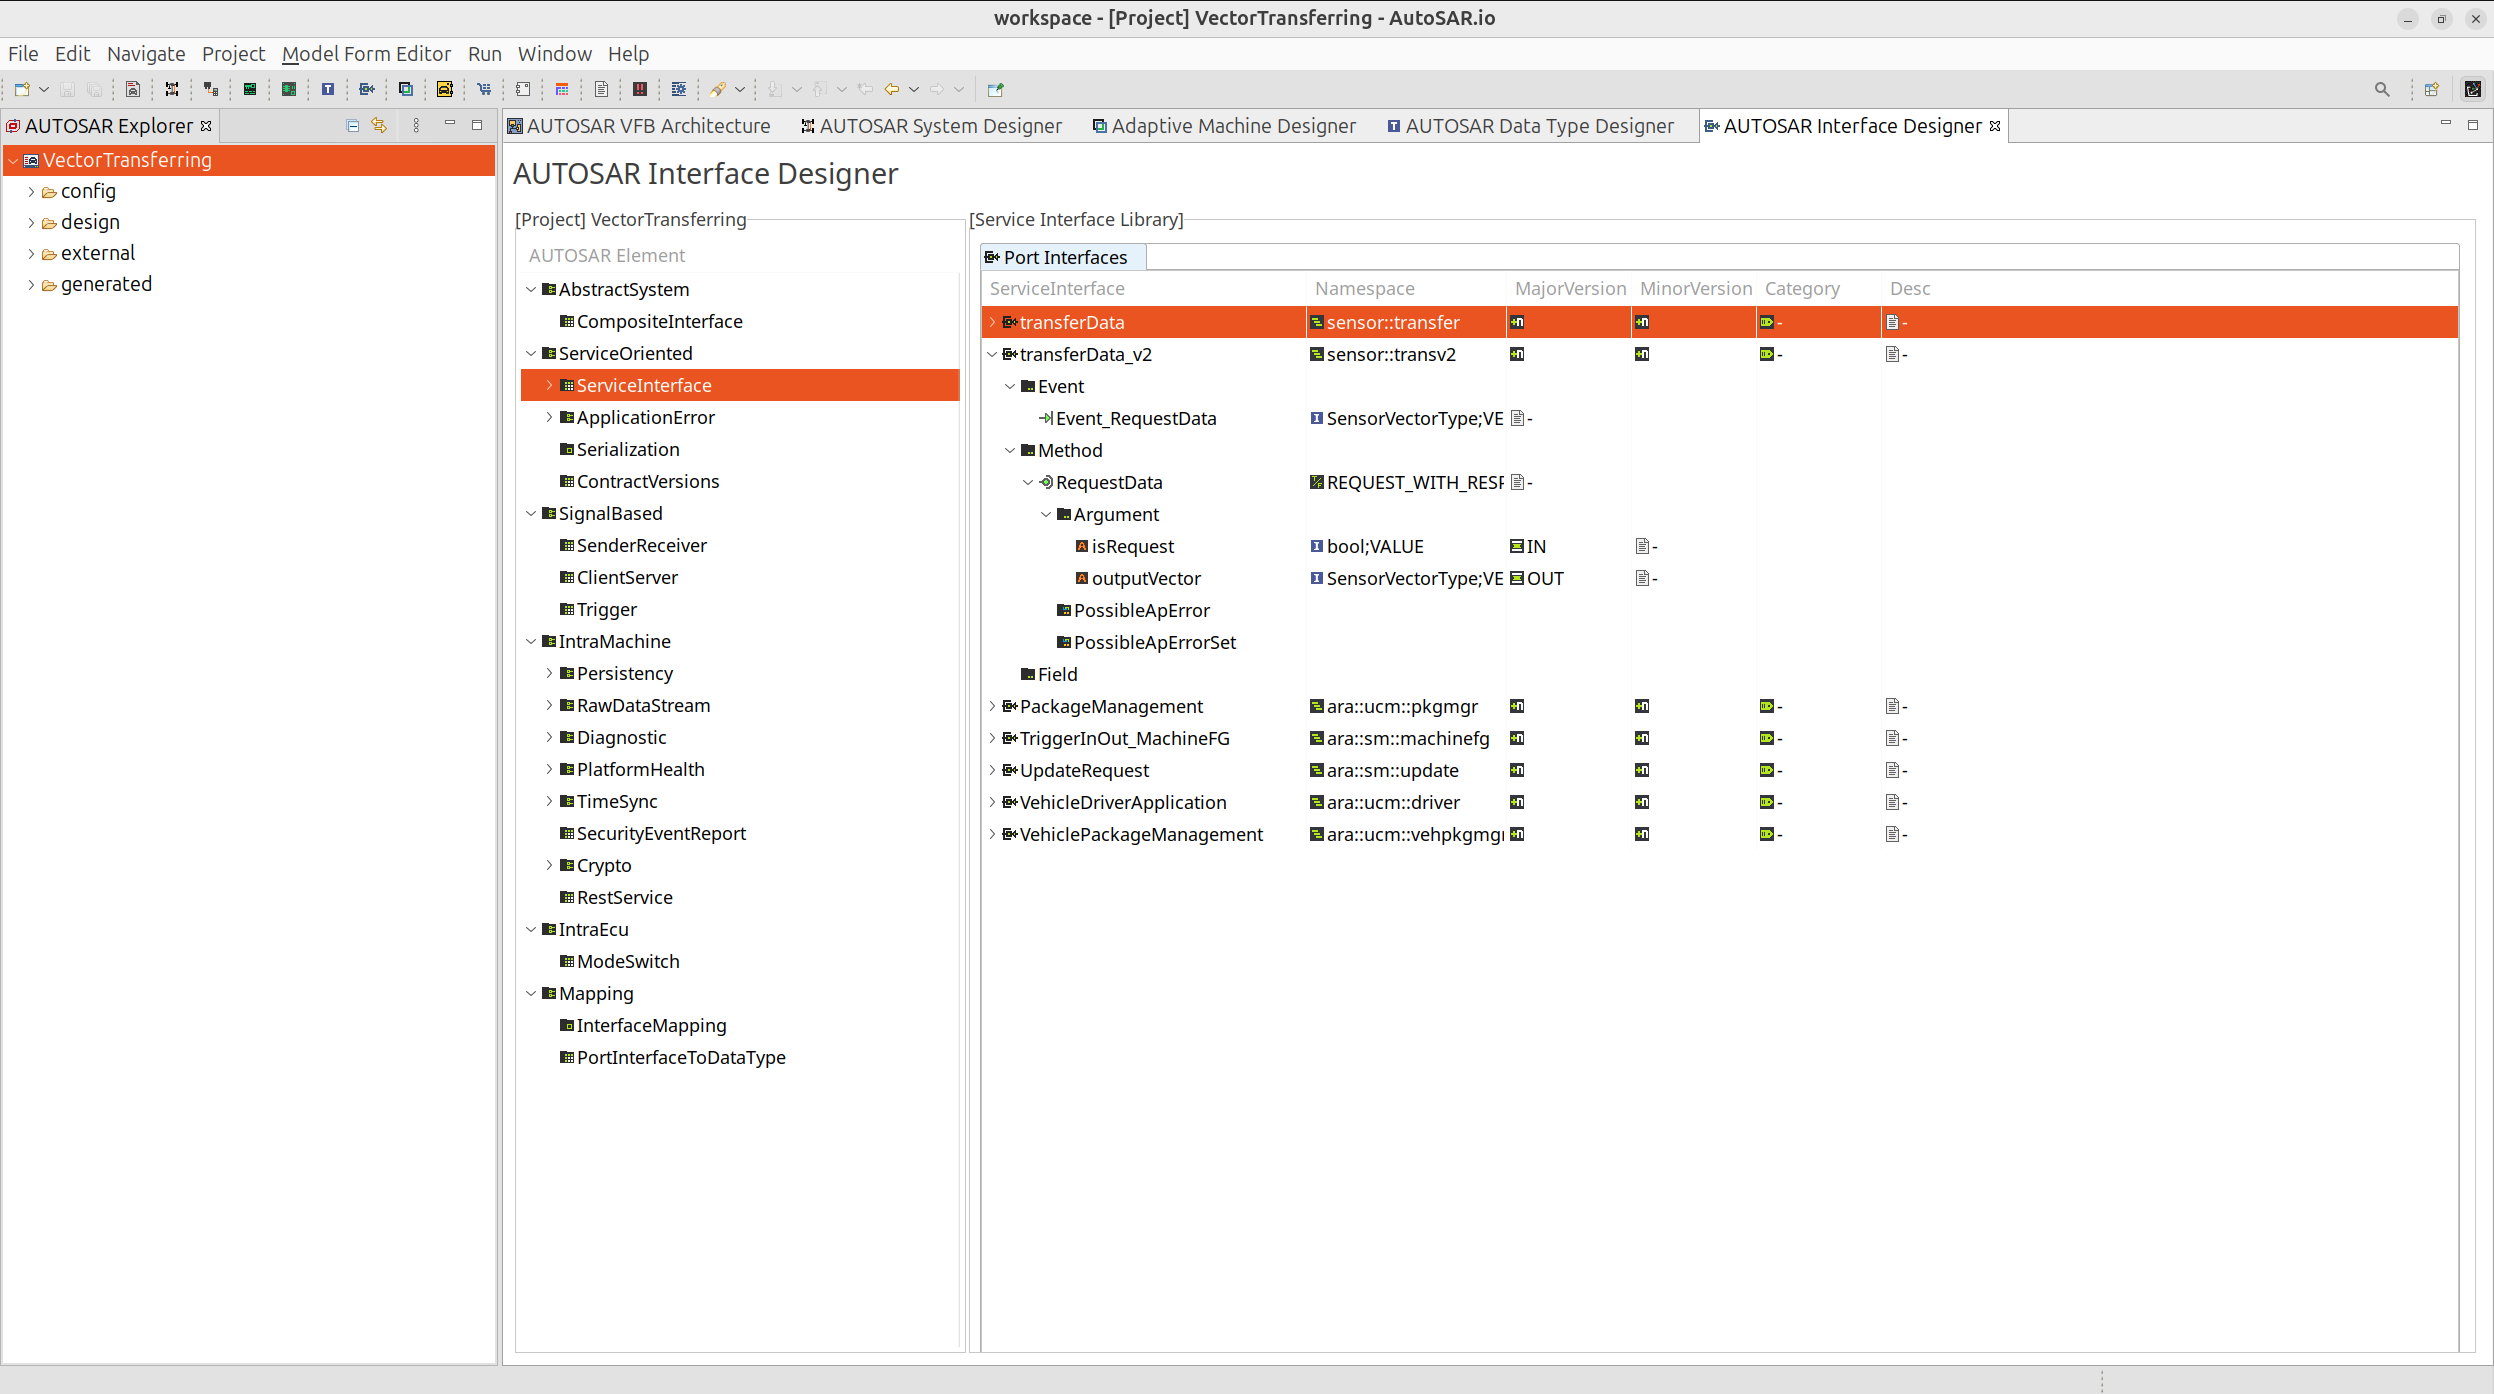
\includegraphics[width=0.75\textwidth]{Images/chap3/image_methodology/serviceInterfaceDesign/defineServiceInterface.png}
    \vspace{0.5cm}
    \caption{Service Interface Definition in Adaptive AUTOSAR}
    \label{fig:service_interface_definition}
\end{figure}

Figure~\ref{fig:service_interface_definition} illustrates the definition of a service oriented interface in the AUTOSAR Interface Designer. The service interface named \texttt{transferData\_v2} is specified within the \texttt{sensor::transv2} namespace and versioned to support interface evolution. It exposes both an event and a method, where the event enables asynchronous notification of data availability, while the method defines a request response interaction pattern for controlled data transmission between applications.

In addition, the interface description includes detailed method arguments and data flow directions. The \texttt{RequestData} method accepts an input parameter that influences the request behavior and produces an output vector based on the previously defined sensor data type. The event is associated with the same data representation (\texttt{Event\_RequestData}), allowing consumers to receive updates without explicitly issuing a request. Possible application errors are also declared to handle exceptional conditions during execution. As shown in Figure~\ref{fig:service_interface_definition}, this interface design supports both reactive and on demand communication between service providers and consumers in the Adaptive AUTOSAR system.


% Service deployment configuration
\begin{figure}[H]
    \centering
    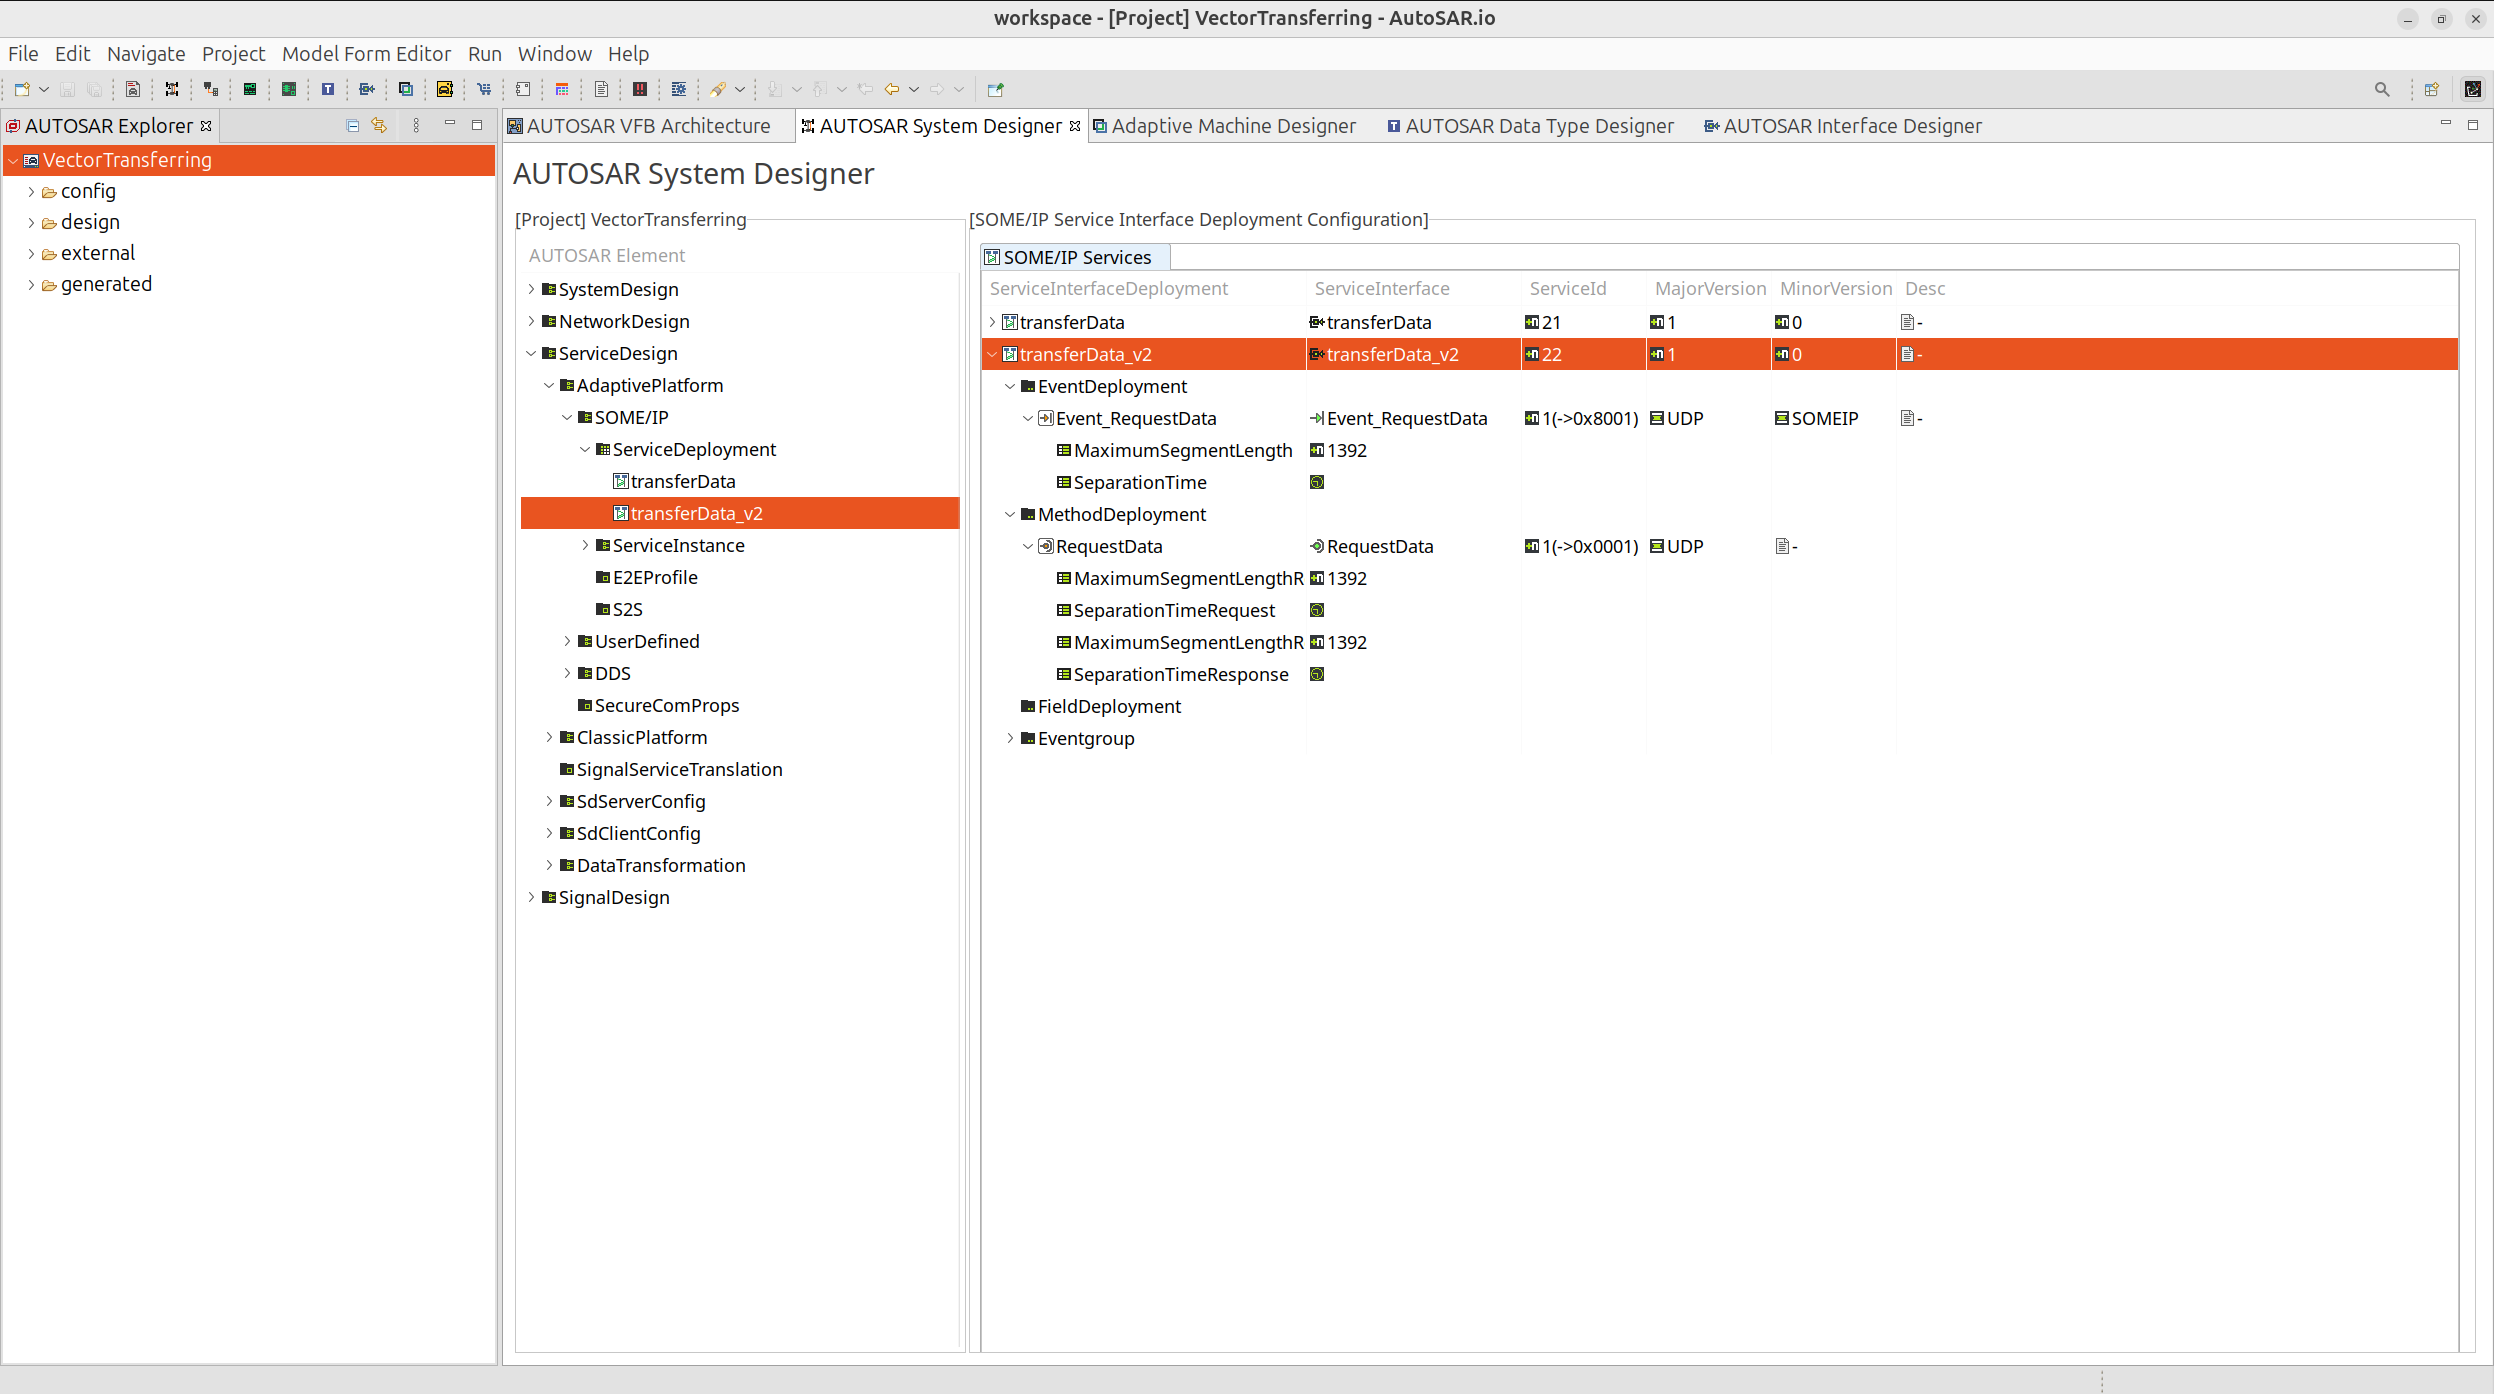
\includegraphics[width=0.75\textwidth]{Images/chap3/image_methodology/serviceInterfaceDesign/serviceDeployment.png}
    \vspace{0.5cm}
    \caption{Service Deployment Configuration}
    \label{fig:service_deployment}
\end{figure}

Figure~\ref{fig:service_deployment} illustrates the SOME/IP service deployment configuration for the \texttt{transferData\_v2} interface within the AUTOSAR System Designer. In this project, the service is explicitly deployed over SOME/IP with transport protocol (SOME/IP-TP) to support the transmission of large data payloads, such as image frames, between the ProviderSensor and ClientSensor applications.

The service is assigned a unique service identifier and version number and includes both event-based and method-based communication. The event \texttt{Event\_RequestData} is configured to use UDP transport together with a specified \texttt{MaximumSegmentLength}. This parameter plays a critical role in enabling SOME/IP-TP, as it informs the Adaptive AUTOSAR middleware that the transmitted data may exceed the maximum payload size of a single UDP packet and therefore must be segmented and reassembled at the receiver side.

Without configuring the \texttt{MaximumSegmentLength}, the communication would default to standard SOME/IP over UDP, which is suitable only for small messages and is not appropriate for transmitting image data. By explicitly defining this parameter, the deployment ensures that image payloads generated by the ProviderSensor are correctly fragmented, transmitted, and reassembled by the ClientSensor.

In addition to the event deployment, the \texttt{RequestData} method deployment specifies request and response timing parameters, supporting controlled client–server interaction when on-demand data transfer is required. Together, these configurations ensure that the \texttt{transferData\_v2} service can be reliably discovered via Service Discovery and can support both event-driven and request-based communication over SOME/IP-TP during runtime execution.


% Service instance provider configuration
\begin{figure}[H]
    \centering
    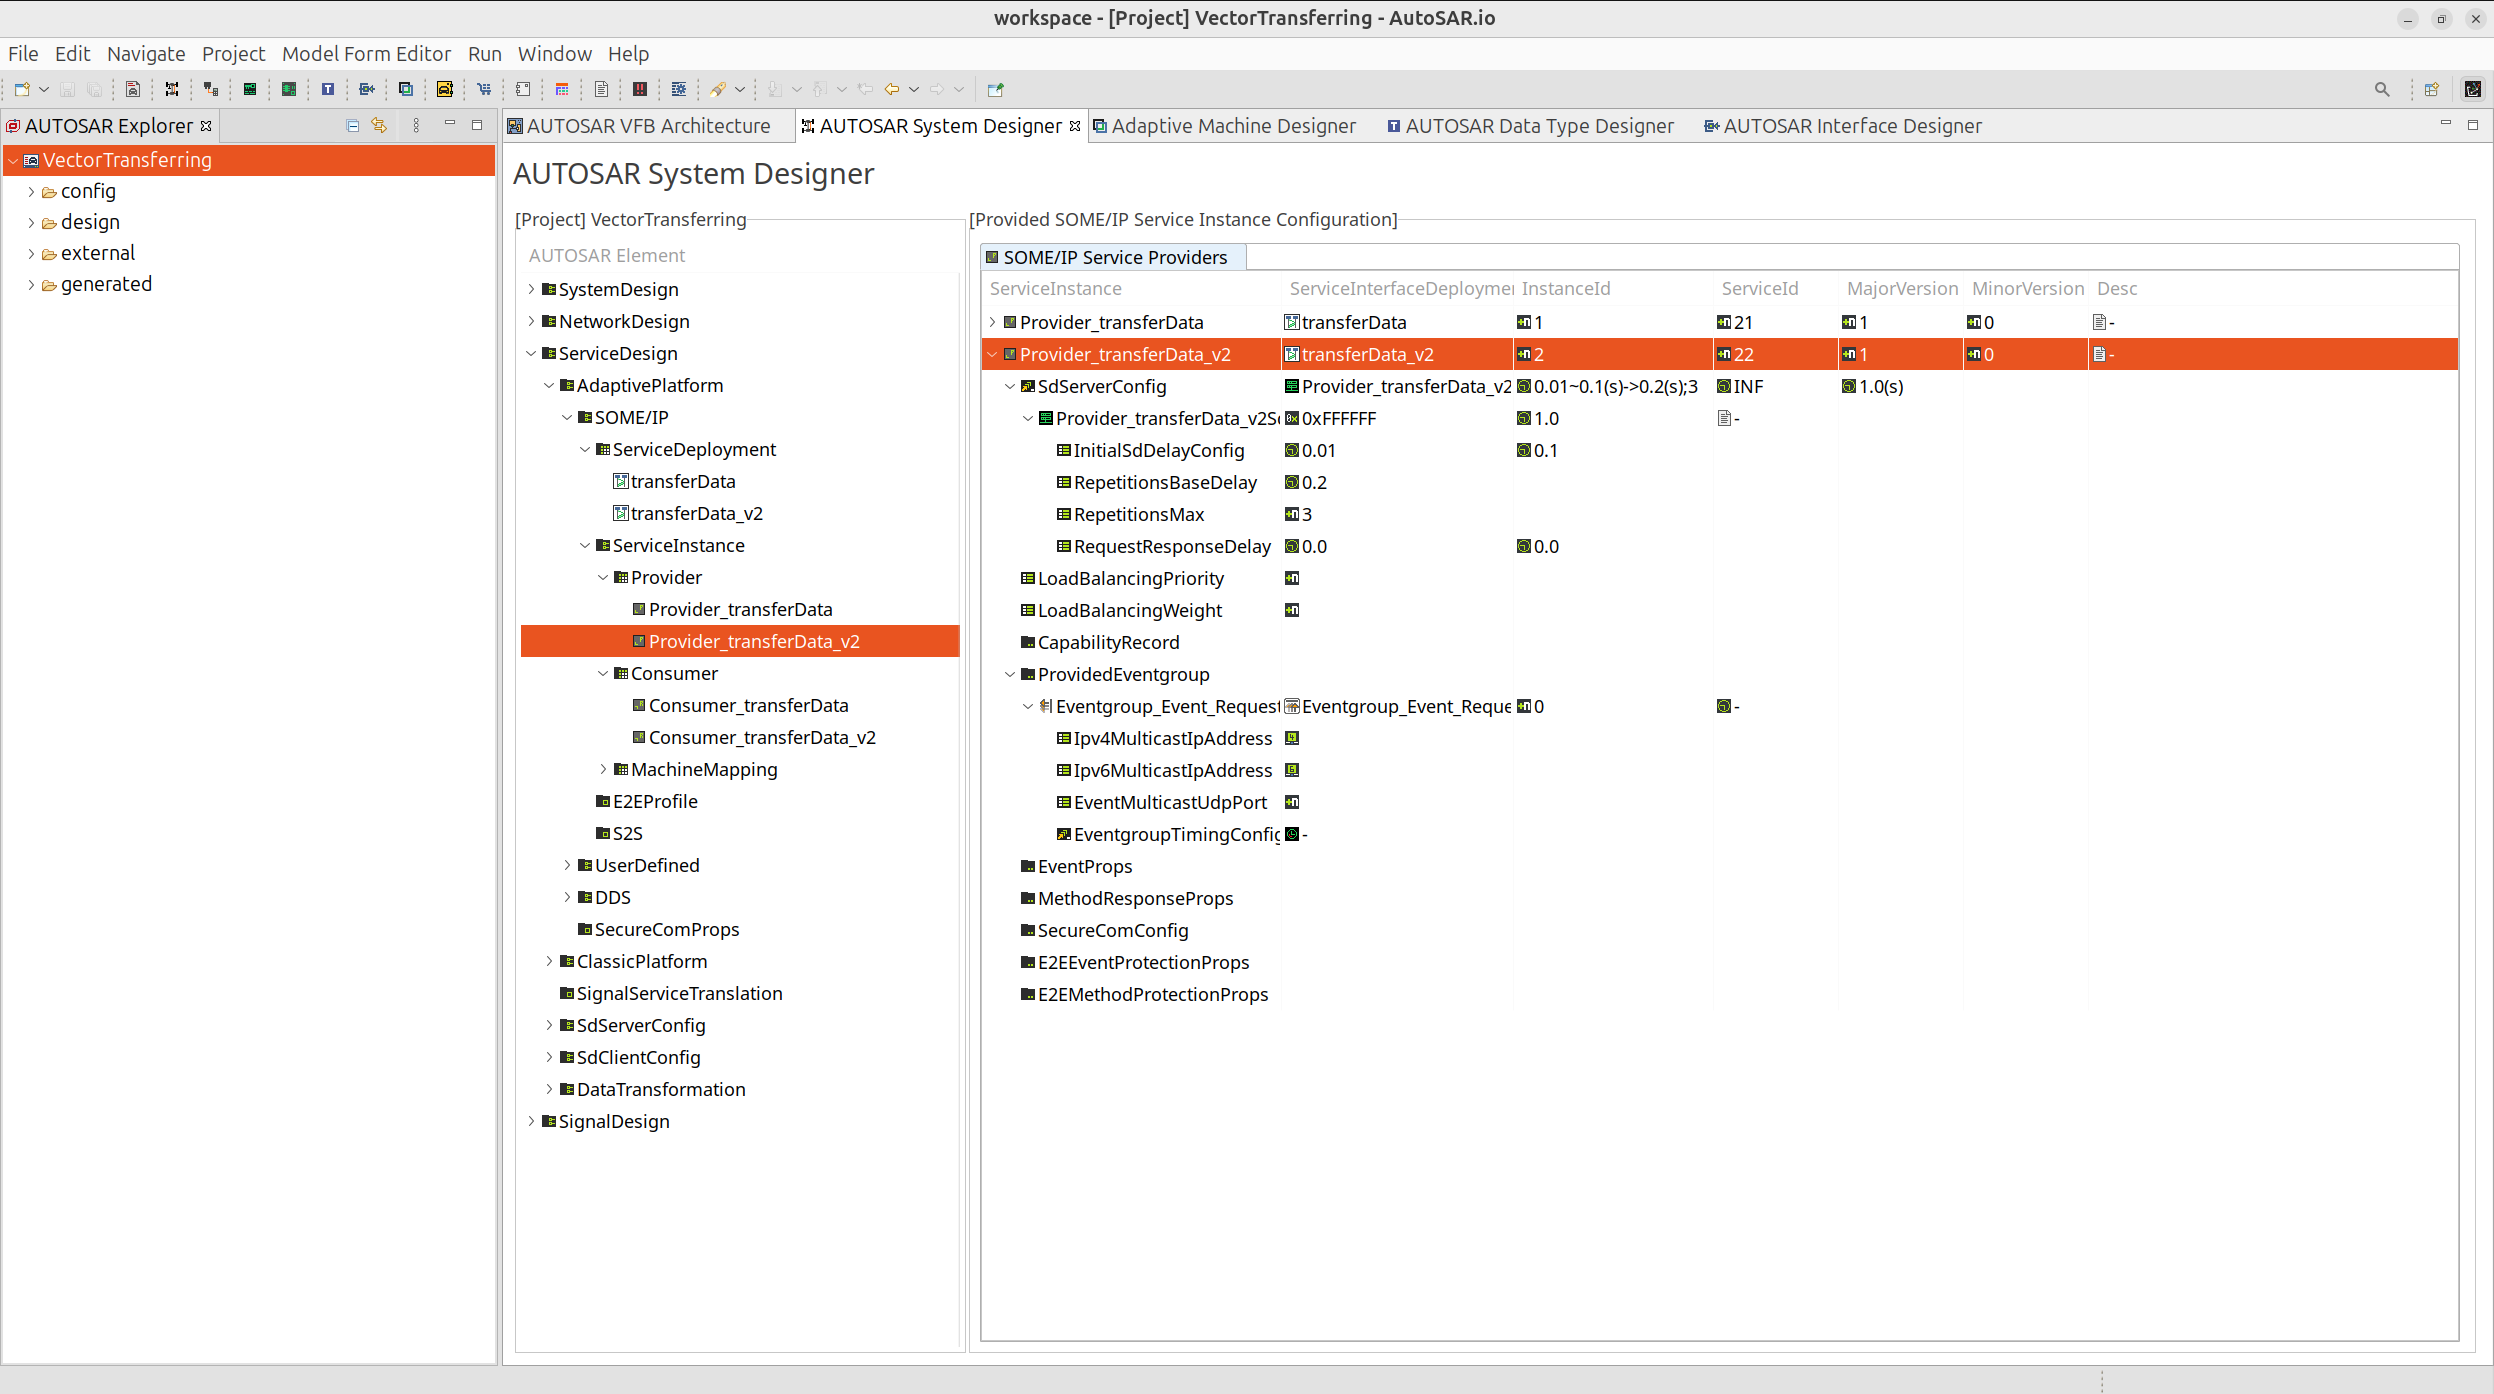
\includegraphics[width=0.75\textwidth]{Images/chap3/image_methodology/serviceInterfaceDesign/serviceInstance_Provider.png}
    \vspace{0.5cm}
    \caption{Service Instance Configuration for Provider}
    \label{fig:service_instance_provider}
\end{figure}

Figure~\ref{fig:service_instance_provider} illustrates the configuration of the SOME/IP service provider for the \texttt{transferData\_v2} interface. The provider instance is bound to a specific service and instance identifier with a defined major and minor version, ensuring compatibility with consuming applications. Server side parameters such as initial service offer delay, repetition base delay, and maximum repetitions are configured to control service availability announcements via Service Discovery. In addition, the provider defines event group settings for data notifications, together with timing and response related properties, which enable reliable dissemination of event based data to subscribed consumers during runtime.

% Service instance consumer configuration
\begin{figure}[H]
    \centering
    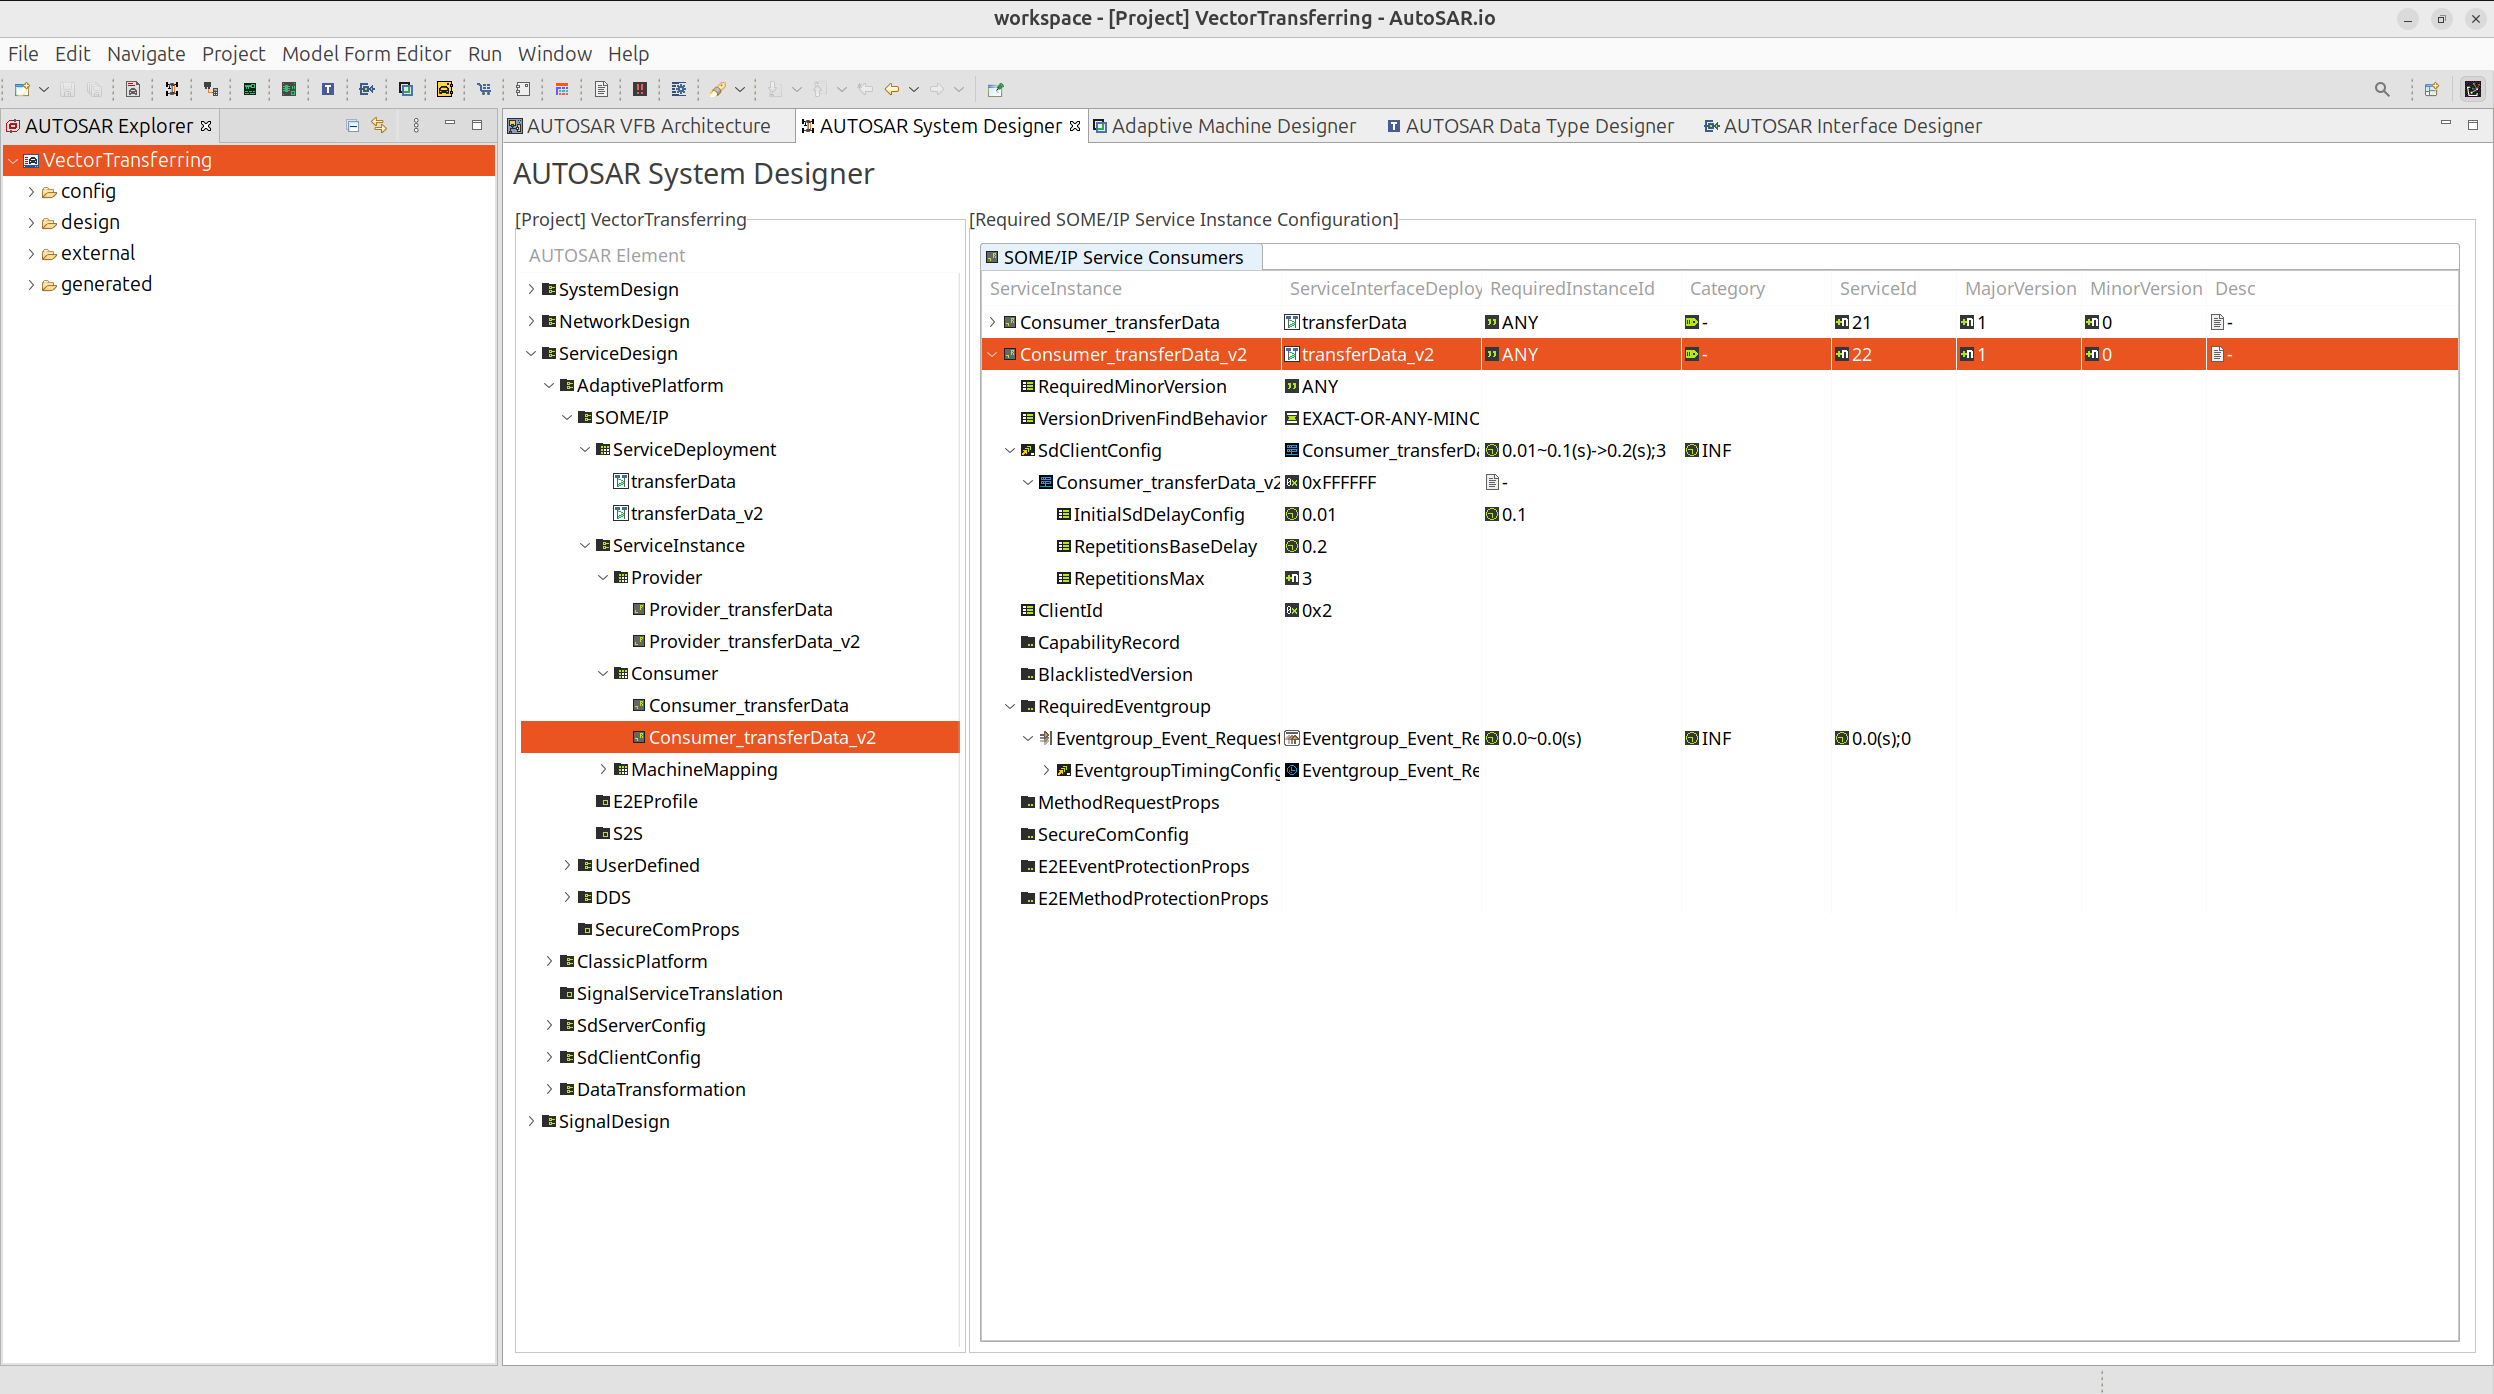
\includegraphics[width=0.75\textwidth]{Images/chap3/image_methodology/serviceInterfaceDesign/serviceInstance_Consumer.png}
    \vspace{0.5cm}
    \caption{Service Instance Configuration for Consumer}
    \label{fig:service_instance_consumer}
\end{figure}

Figure~\ref{fig:service_instance_consumer} presents the configuration of the corresponding SOME/IP service consumer acting as a subscriber to the \texttt{transferData\_v2} service. The consumer specifies flexible version requirements and discovery behavior, allowing it to bind to compatible provider instances at runtime. Client side parameters such as initial request delay, repetition strategy, and event group subscription settings determine how the consumer discovers the service and receives event notifications. Through this configuration, the consumer can dynamically subscribe to published data while maintaining controlled request and subscription behavior within the Adaptive AUTOSAR communication framework.

% Mapping service to machine network endpoint
\begin{figure}[H]
    \centering
    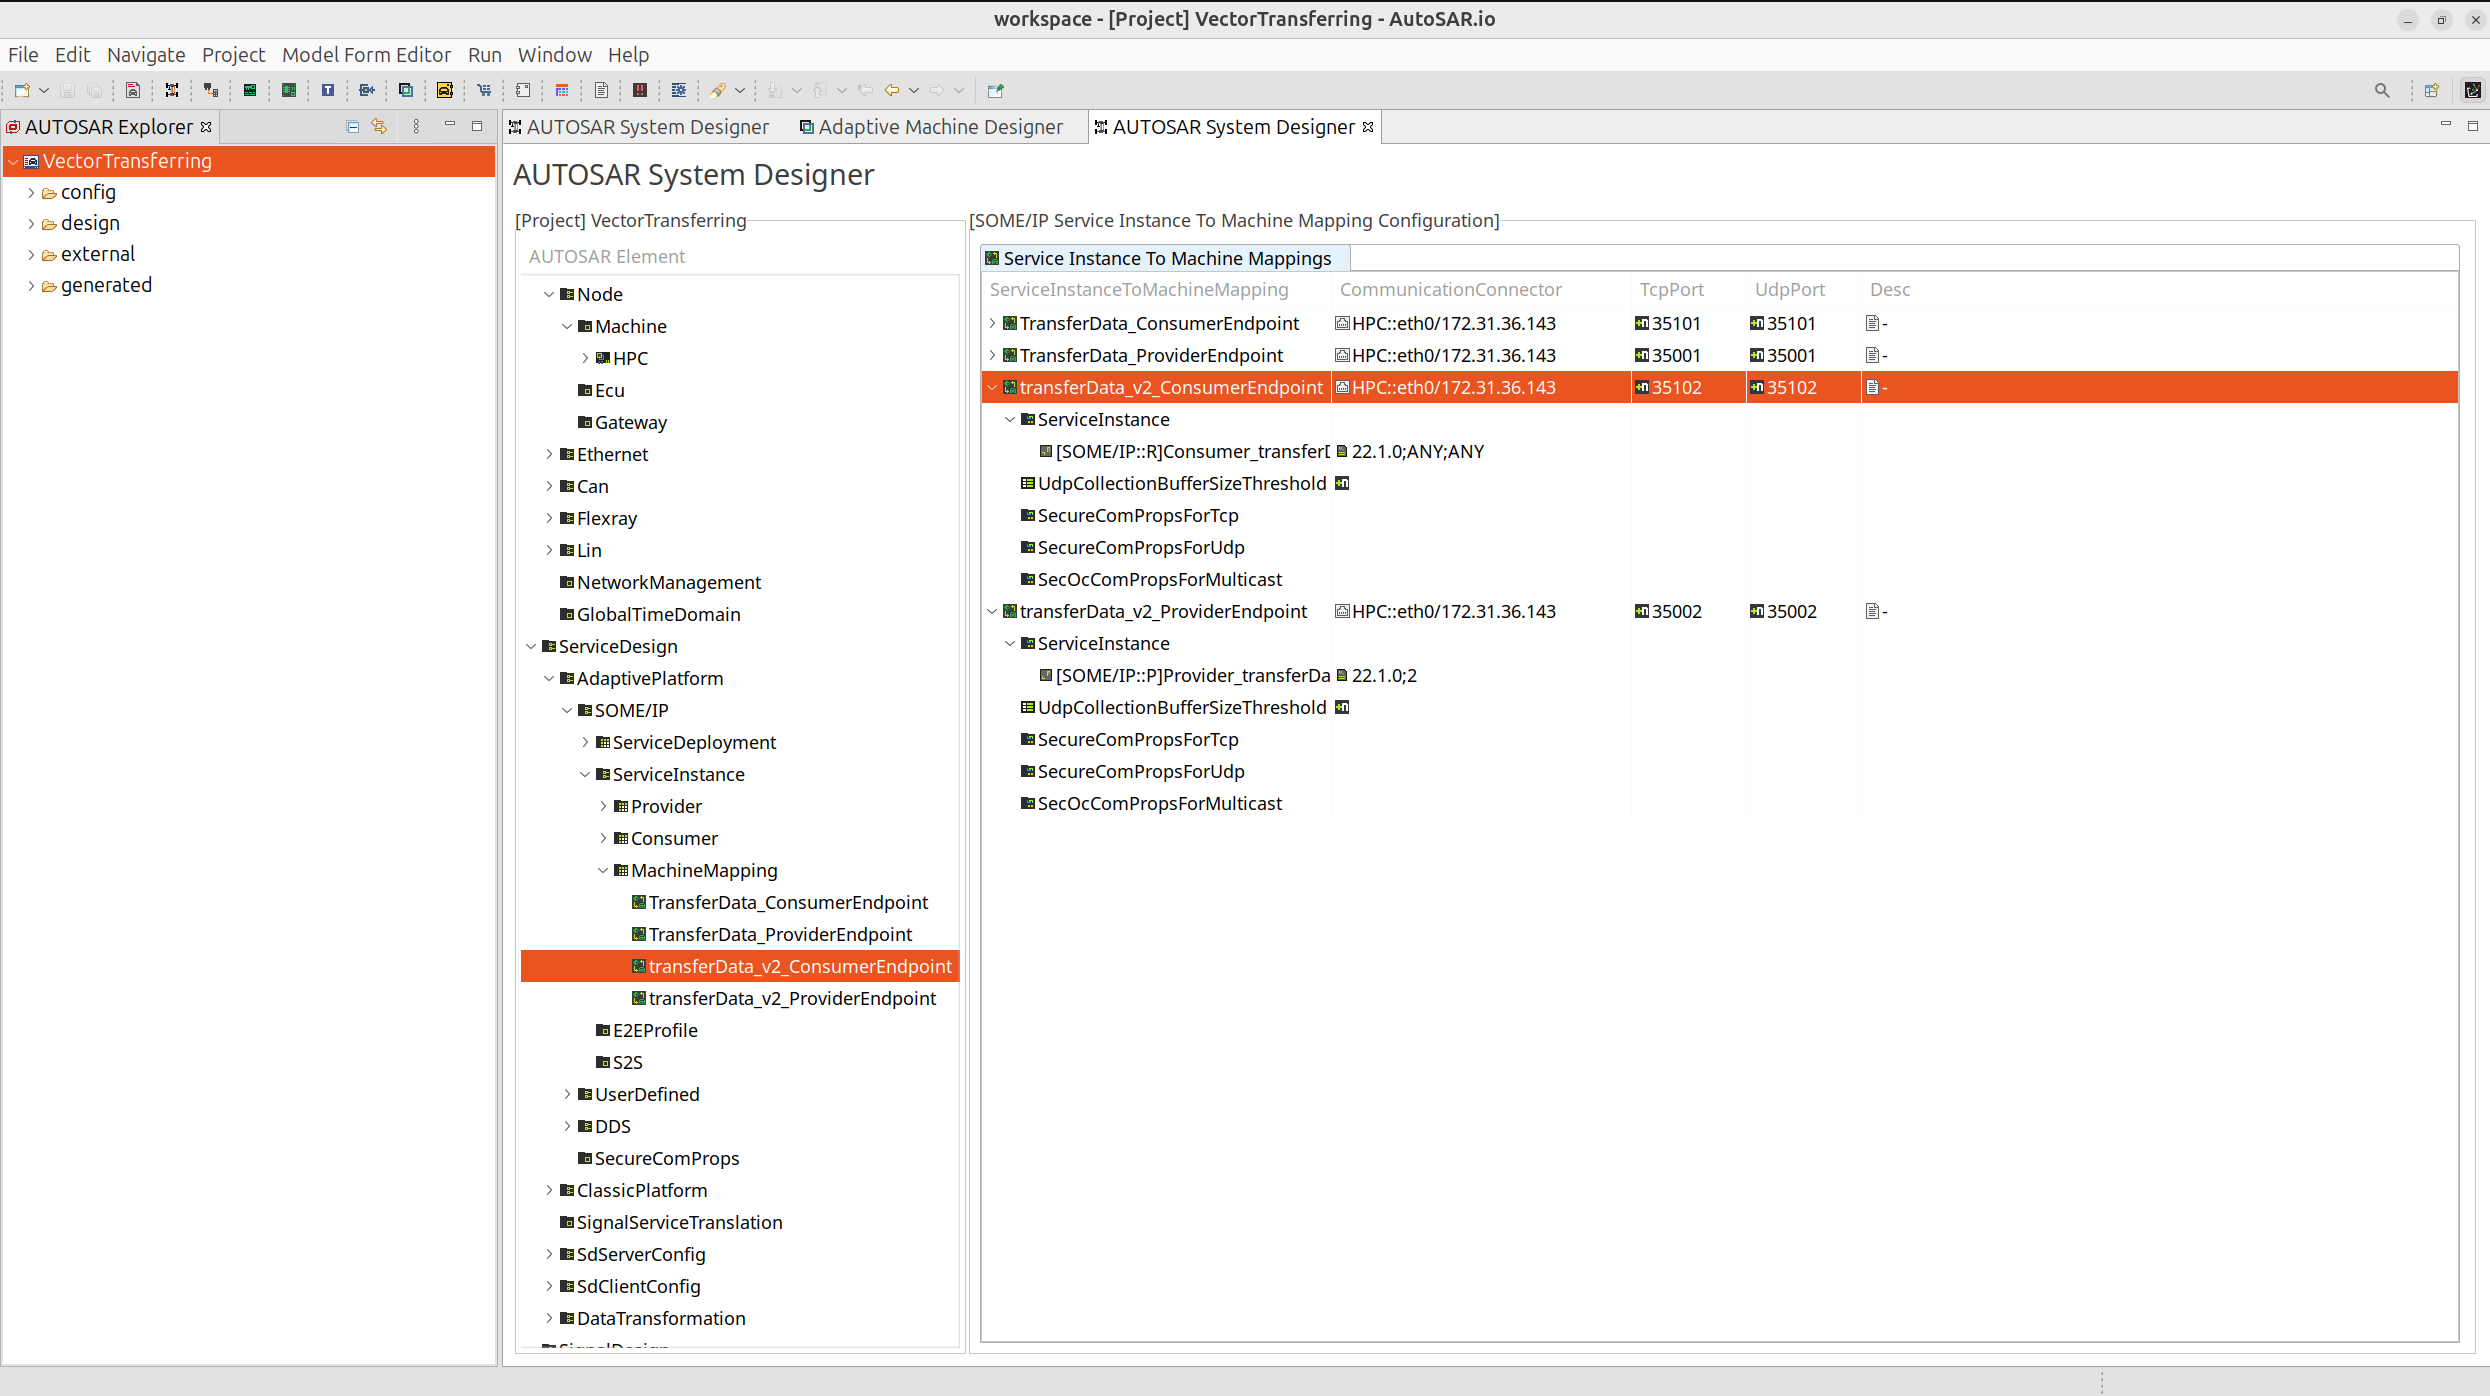
\includegraphics[width=0.75\textwidth]{Images/chap3/image_methodology/serviceInterfaceDesign/serviceMappingMachineEndpoint.png}
    \vspace{0.5cm}
    \caption{Mapping Service Instances to Machine Network Endpoint}
    \label{fig:service_machine_endpoint_mapping}
\end{figure}

Figure~\ref{fig:service_machine_endpoint_mapping} illustrates how the service instances of the \texttt{transferData} and \texttt{transferData\_v2} interfaces are bound to concrete machine network endpoints. Both provider and consumer instances are mapped to the Ethernet communication connector \texttt{HPC:eth0} with the fixed IPv4 address \texttt{172.31.36.143}, ensuring that all service communication is routed through a well defined network interface. Distinct TCP and UDP port numbers are assigned to each service instance, allowing concurrent data exchange while avoiding port conflicts.

This mapping explicitly links abstract service definitions to physical network resources, enabling correct runtime deployment and communication over SOME/IP. By defining separate endpoints for provider and consumer roles, the configuration supports clear role separation and reliable message routing between applications deployed on the same machine or across different nodes in the Adaptive AUTOSAR system.

\begin{figure}[H]
    \centering
    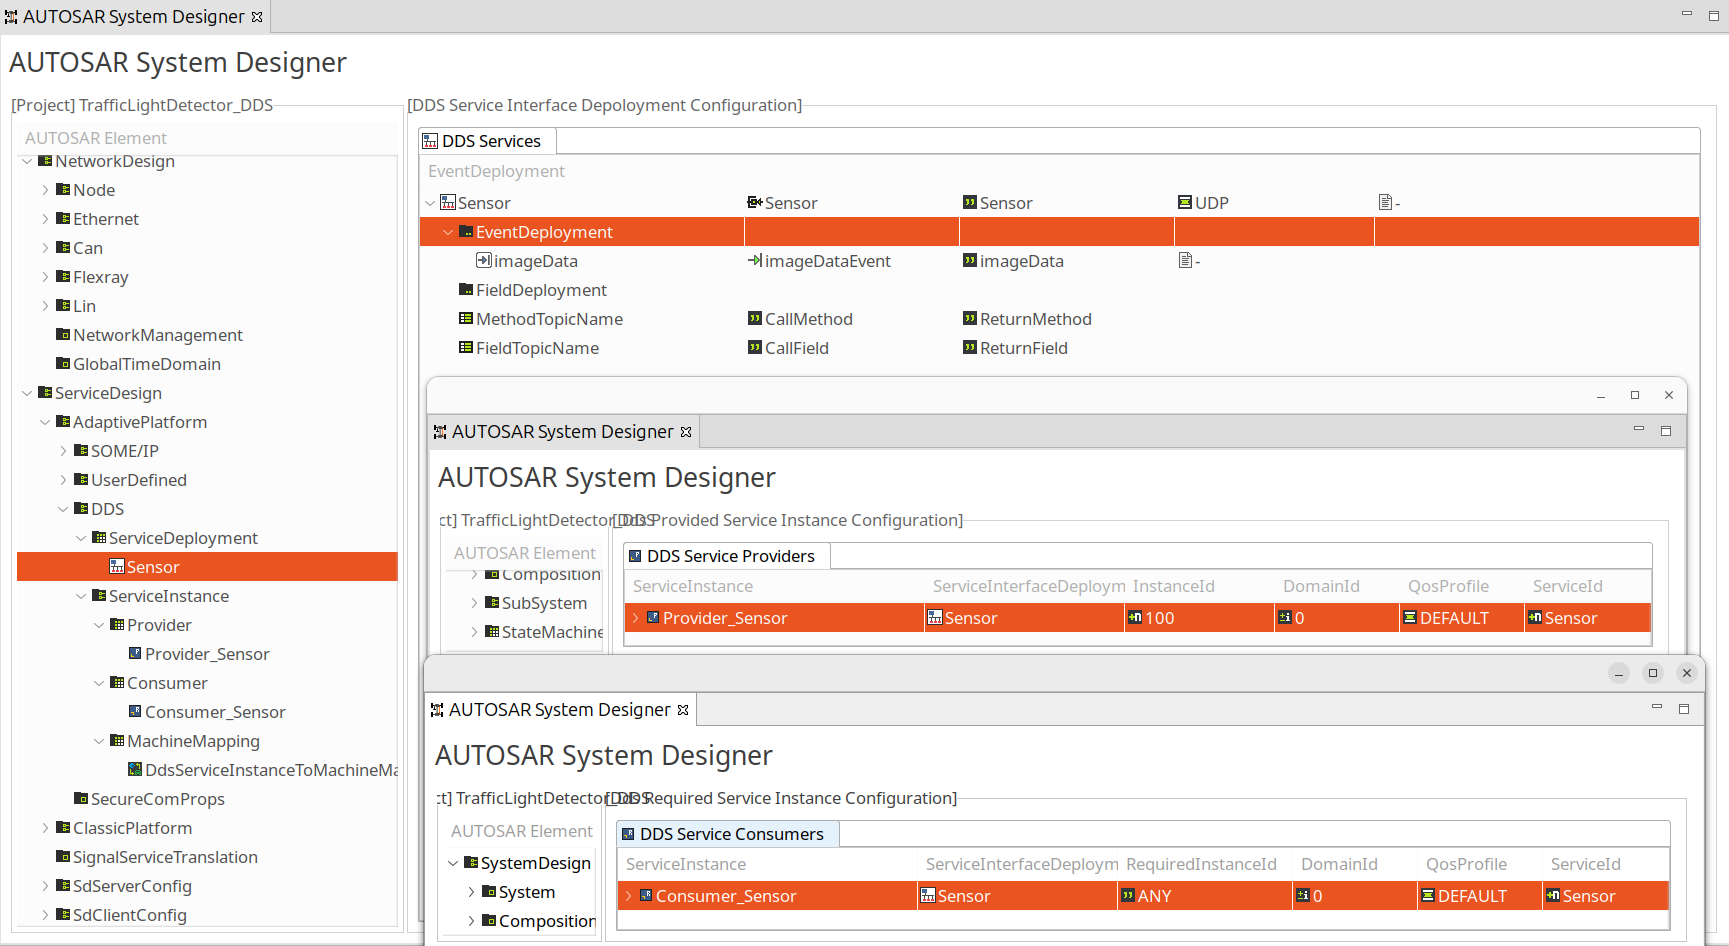
\includegraphics[width=0.75\textwidth]{Images/chap3/image_methodology/serviceInterfaceDesign/DDS_Config.png}
    \vspace{0.5cm}
    \caption{Mapping Service Instances to Machine Network Endpoint}
    \label{fig:dds_config}
\end{figure}

Similarly to the SOME/IP configuration, Figure~\ref{fig:dds_config} presents the DDS-based deployment configuration used for the \texttt{Sensor} service. In the DDS Service Interface Deployment Configuration, the service interface is deployed with the \texttt{imageDataEvent} event and the corresponding DDS topic \texttt{imageData}. The event deployment is configured to use UDP transport, allowing the Provider and Client applications to exchange image and metadata payloads through DDS publish/subscribe communication.

The provided service instance is configured as \texttt{Provider\_Sensor}, bound to the \texttt{Sensor} service deployment with instance-id~\texttt{100}, DDS Domain Id~\texttt{0}, and the \texttt{DEFAULT} QoS profile. The required service instance is configured as \texttt{Consumer\_Sensor}, also bound to the same \texttt{Sensor} service deployment, but with required instance-id~\texttt{ANY}. This configuration allows the Client application to discover and subscribe to the Provider service instance dynamically within the same DDS domain.

Through this DDS configuration, the abstract AUTOSAR service definition is mapped to concrete DDS communication entities, including service deployment, topic, event, provider instance, consumer instance, domain identifier, and QoS profile. This mapping is essential for the implemented prototype because the runtime communication between \texttt{ProviderSensor} and \texttt{ClientSensor} is realized through DDS rather than SOME/IP. As a result, the system can publish \texttt{imageDataEvent} samples on the \texttt{imageData} topic and deliver the \texttt{GpsJpegWireHeader + JPEG} payload from the Provider to the Client in a service-oriented and configurable manner.

\subsubsection{Application Design}

% Modeling Adaptive Application
\begin{figure}[H]
    \centering
    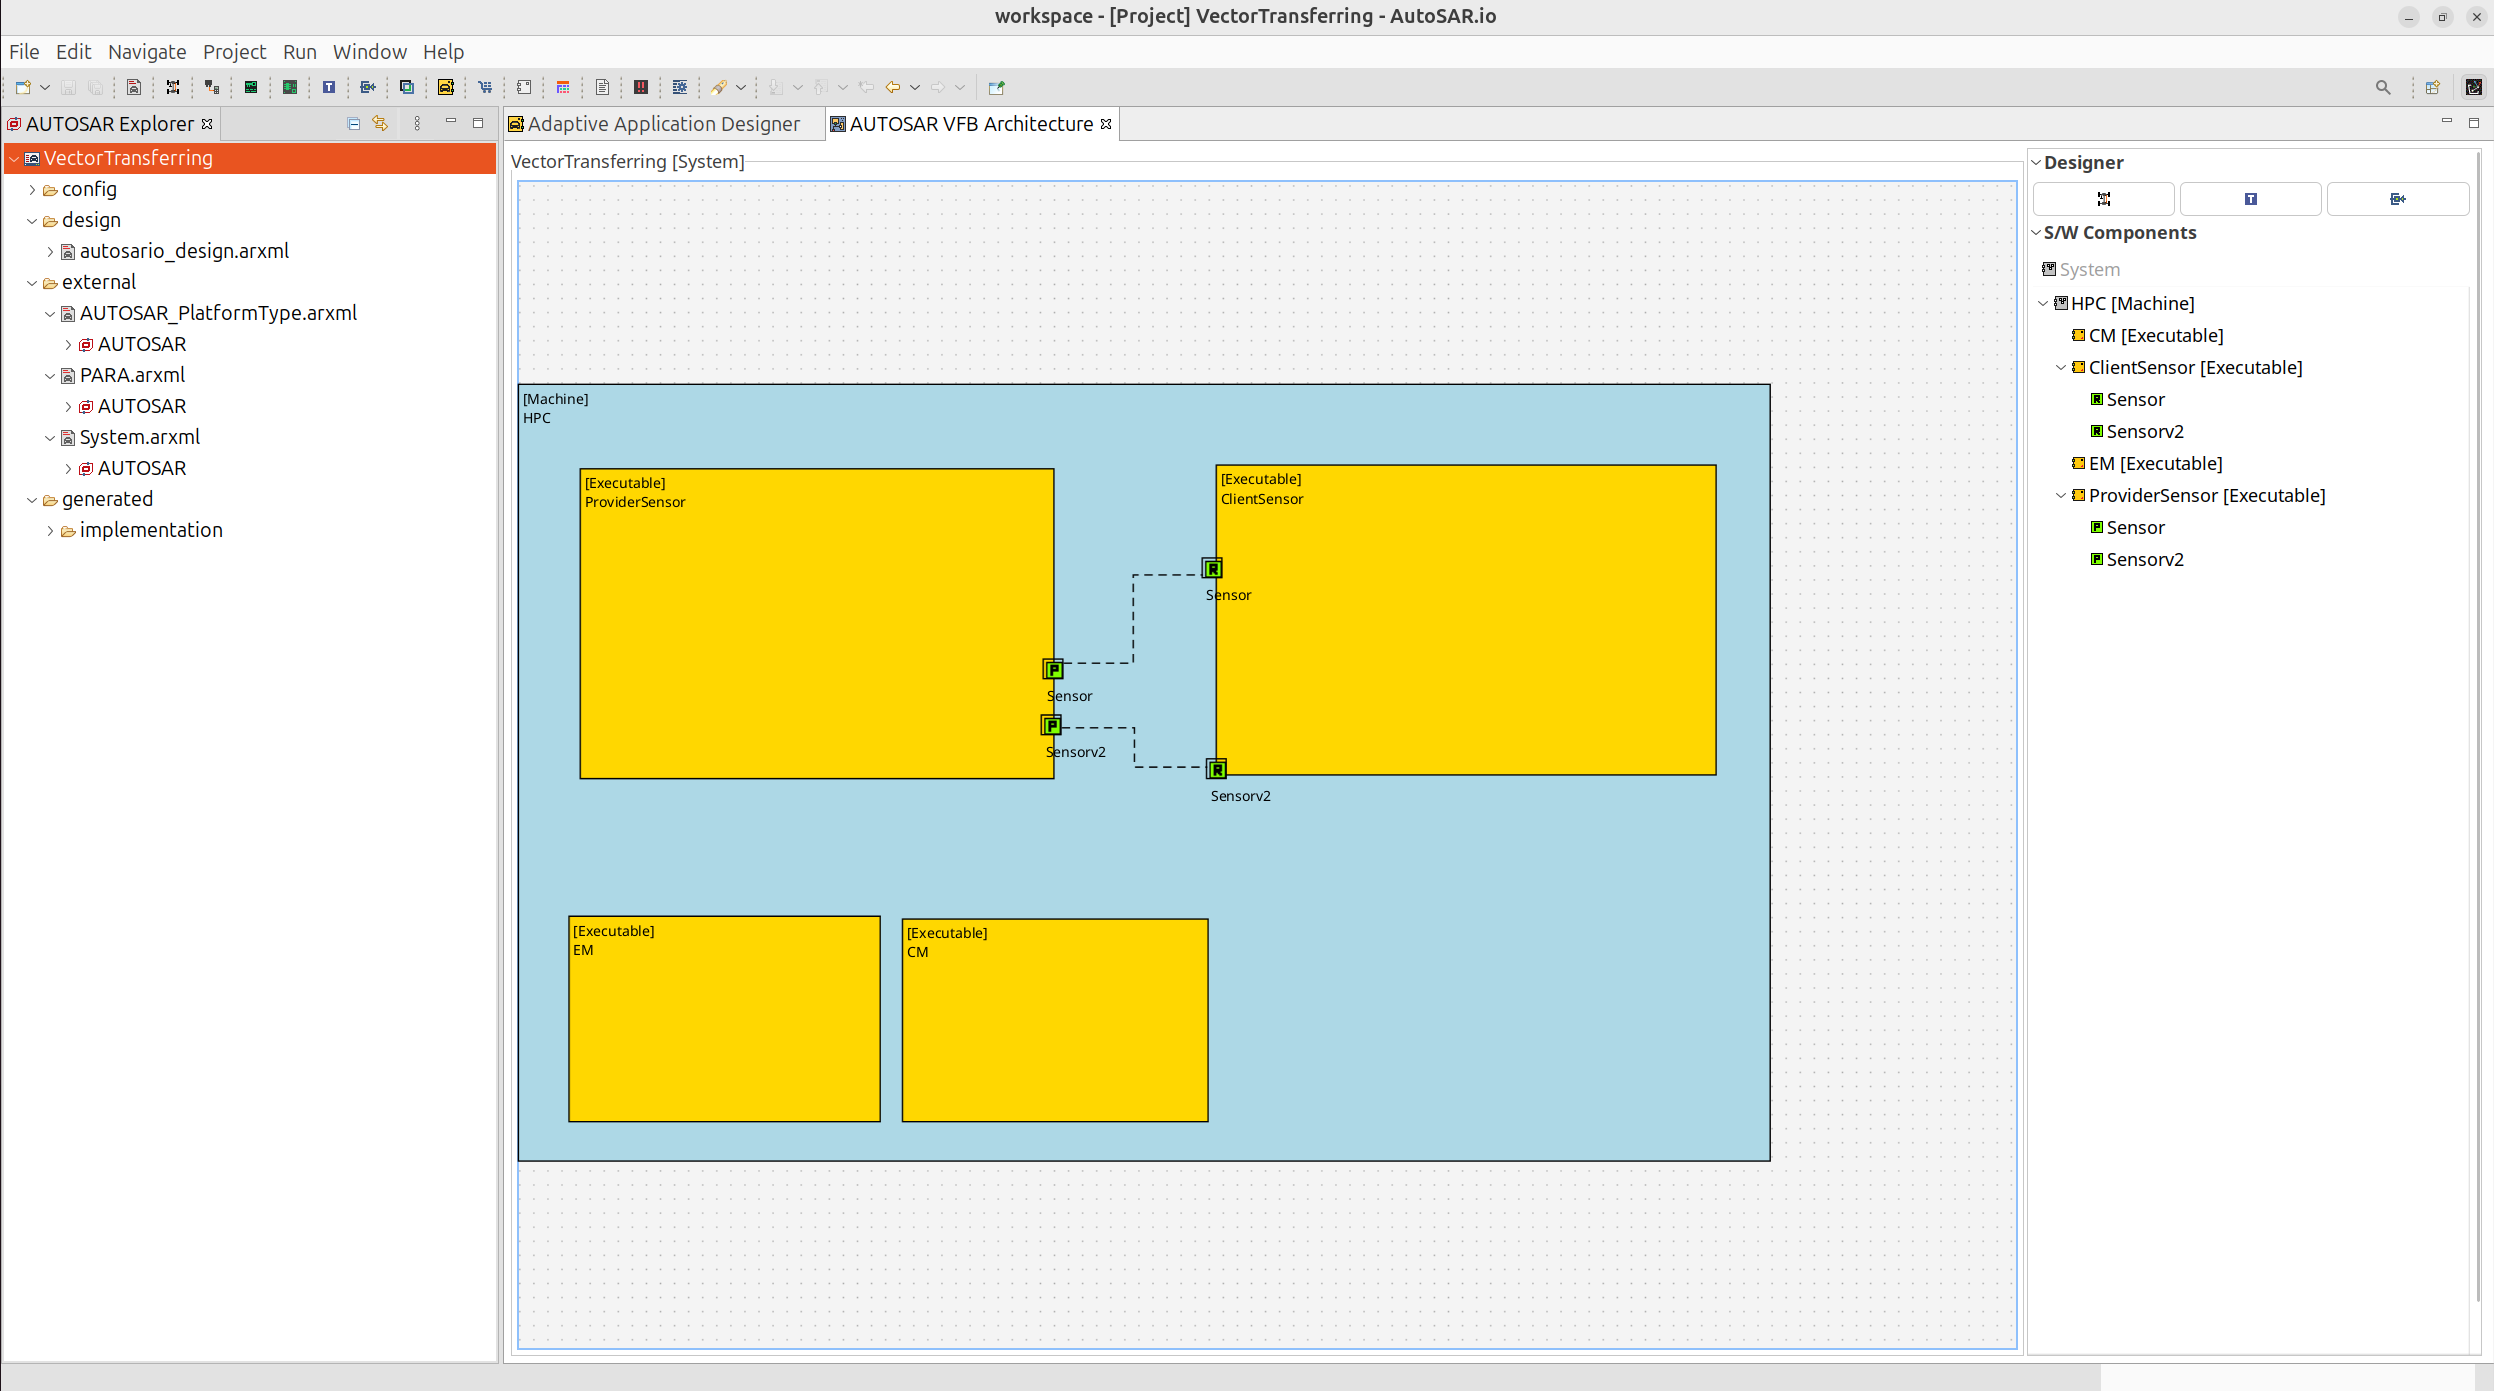
\includegraphics[width=0.75\textwidth]{Images/chap3/image_methodology/applicationDesign/modelingApplication.png}
    \vspace{0.5cm}
    \caption{Modeling of Adaptive Application}
    \label{fig:modeling_application}
\end{figure}

Figure~\ref{fig:modeling_application} shows the Adaptive Application modeling view, where users define the overall application architecture by assigning application executables to a specific machine. In this workspace, the target machine \texttt{HPC} is selected as the deployment context, and multiple executables such as \texttt{ProviderSensor}, \texttt{ClientSensor}, \texttt{CM}, and \texttt{EM} are instantiated within it. Logical connections between executables are visually represented through ports, allowing designers to describe interaction relationships at the architectural level. This model serves as a central design step that links application executables with the underlying machine, providing a clear and structured representation of how software components are organized and deployed in an Adaptive AUTOSAR system.


% Configure Provider Executable Properties
\begin{figure}[H]
    \centering
    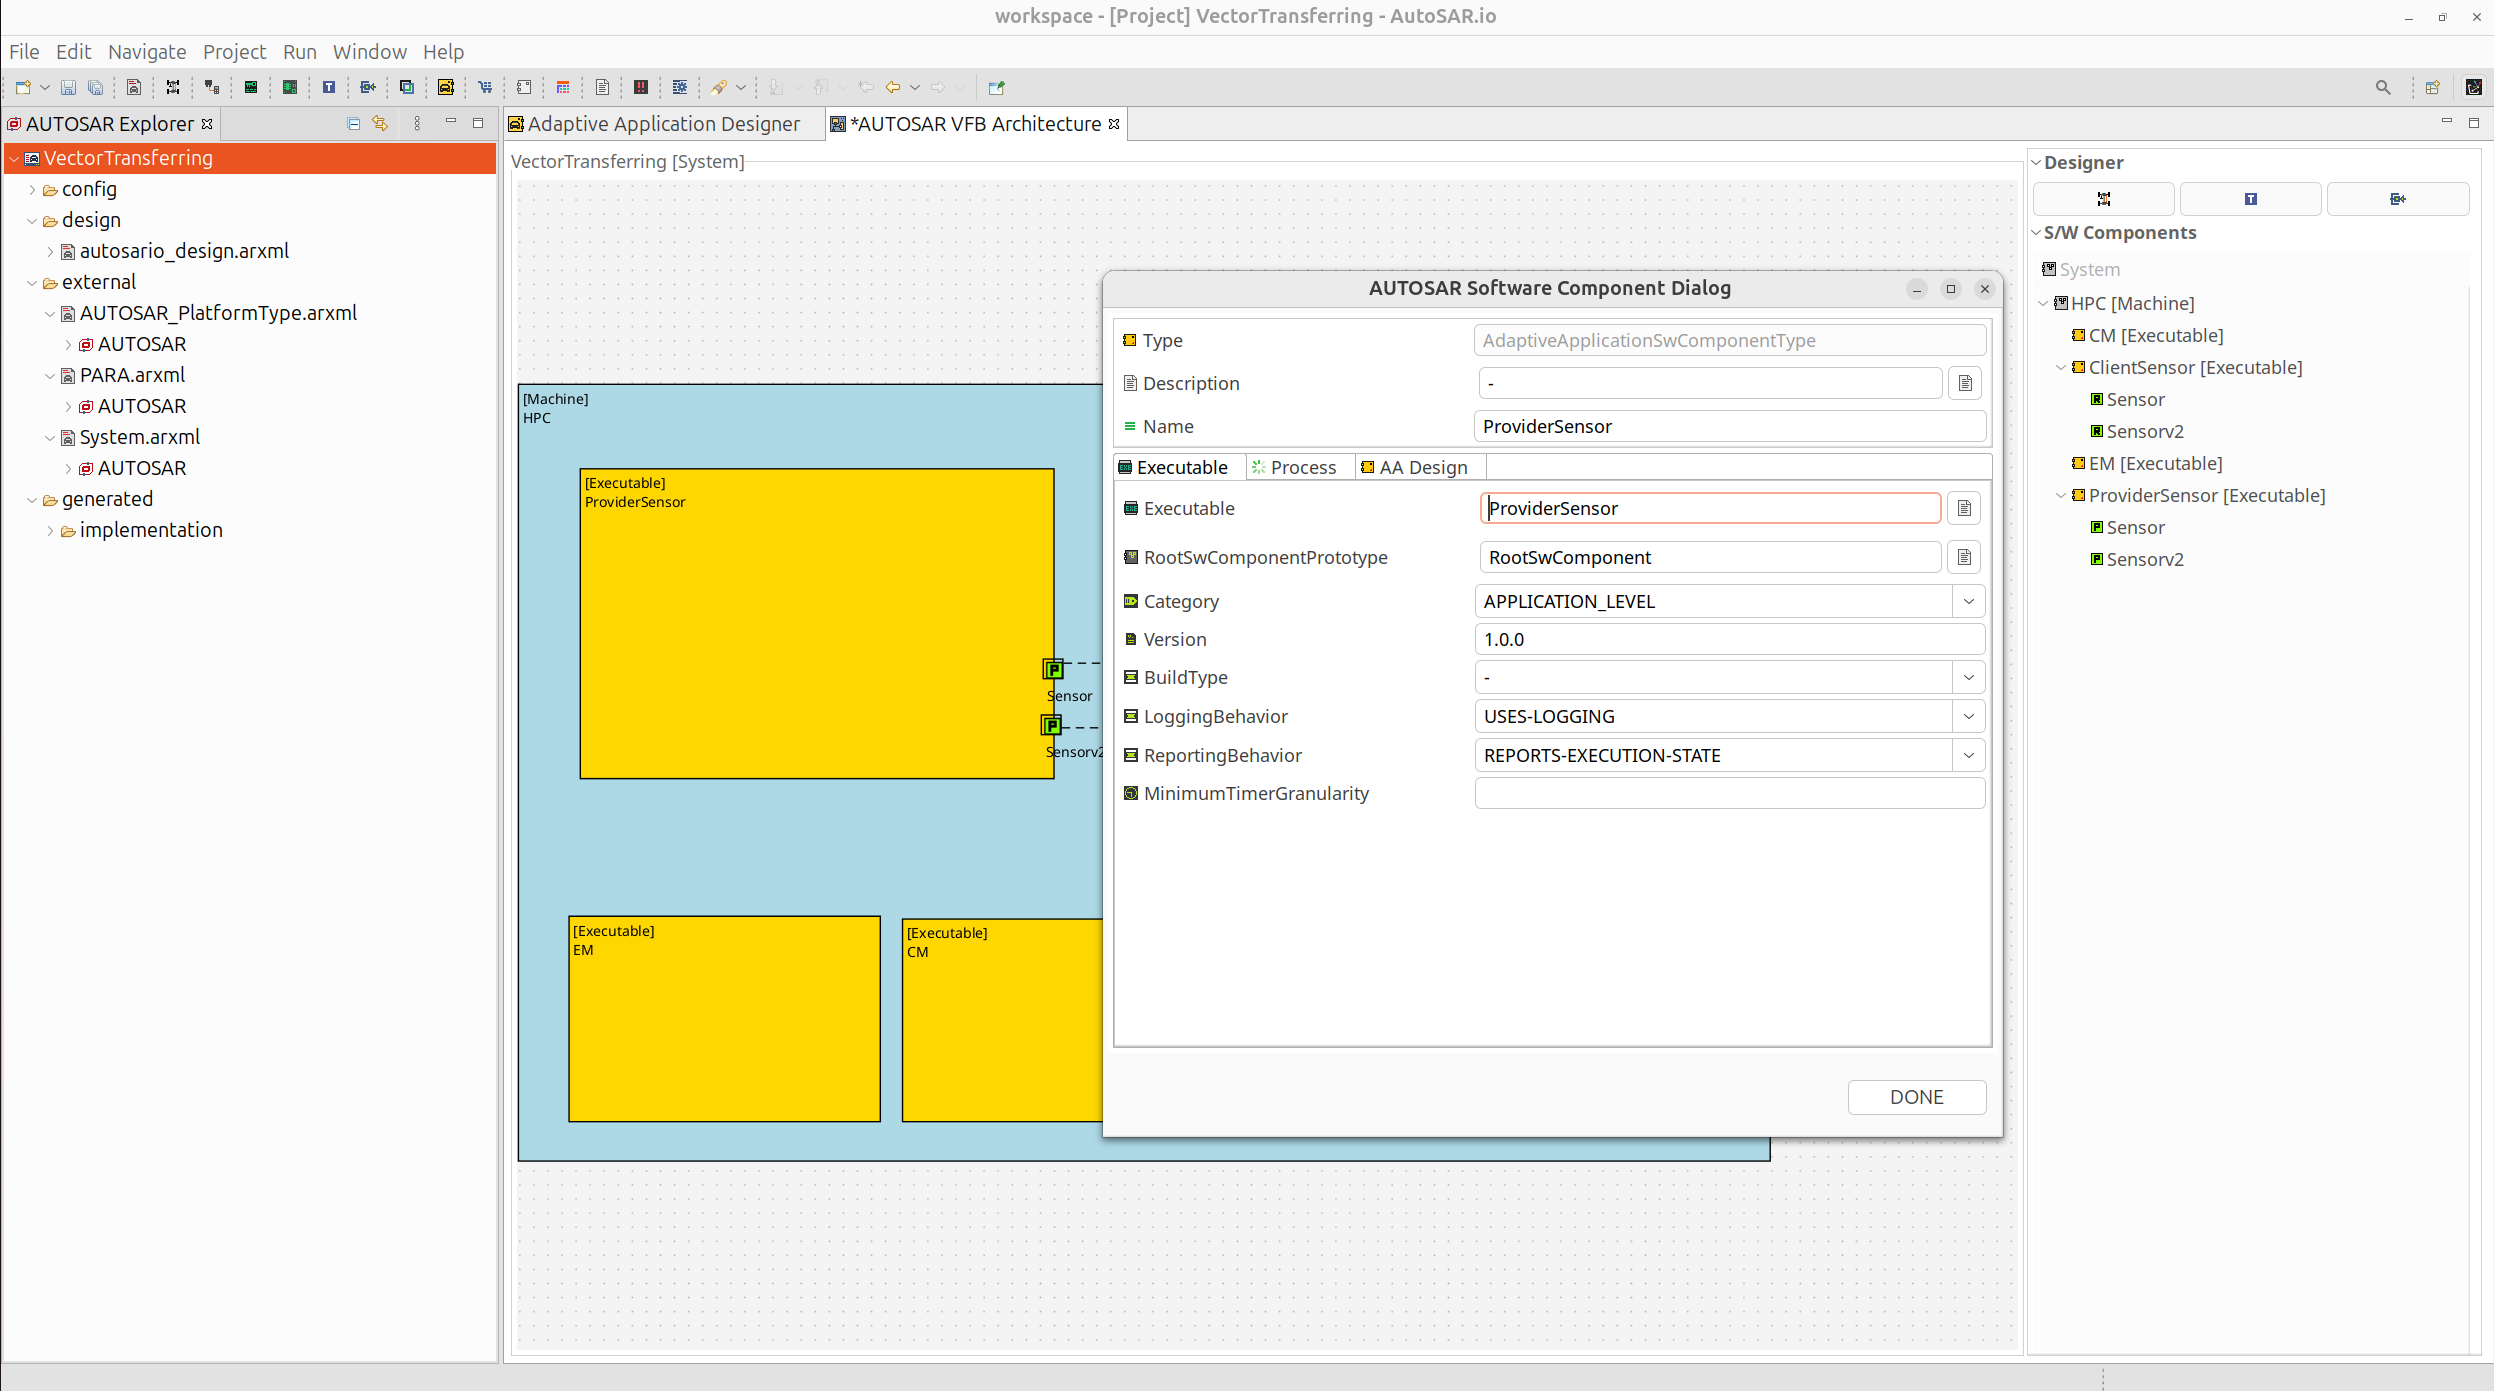
\includegraphics[width=0.75\textwidth]{Images/chap3/image_methodology/applicationDesign/providerExProperties.png}
    \vspace{0.5cm}
    \caption{Configuration of Provider Executable Properties}
    \label{fig:app_provider_executable_properties}
\end{figure}

Figure~\ref{fig:app_provider_executable_properties} presents the configuration of the provider application executable within the Adaptive Application Designer. In this view, the executable \texttt{ProviderSensor} is defined as an application level software component with a specific version and logging behavior. Key properties such as execution category, reporting behavior, and minimum timer granularity are configured to control runtime characteristics and observability. By assigning these attributes, the provider executable is clearly identified as a service offering entity and is prepared to integrate with the Adaptive AUTOSAR execution environment in a consistent and manageable manner.

% Map Provider Ports to Service Interface
\begin{figure}[H]
    \centering
    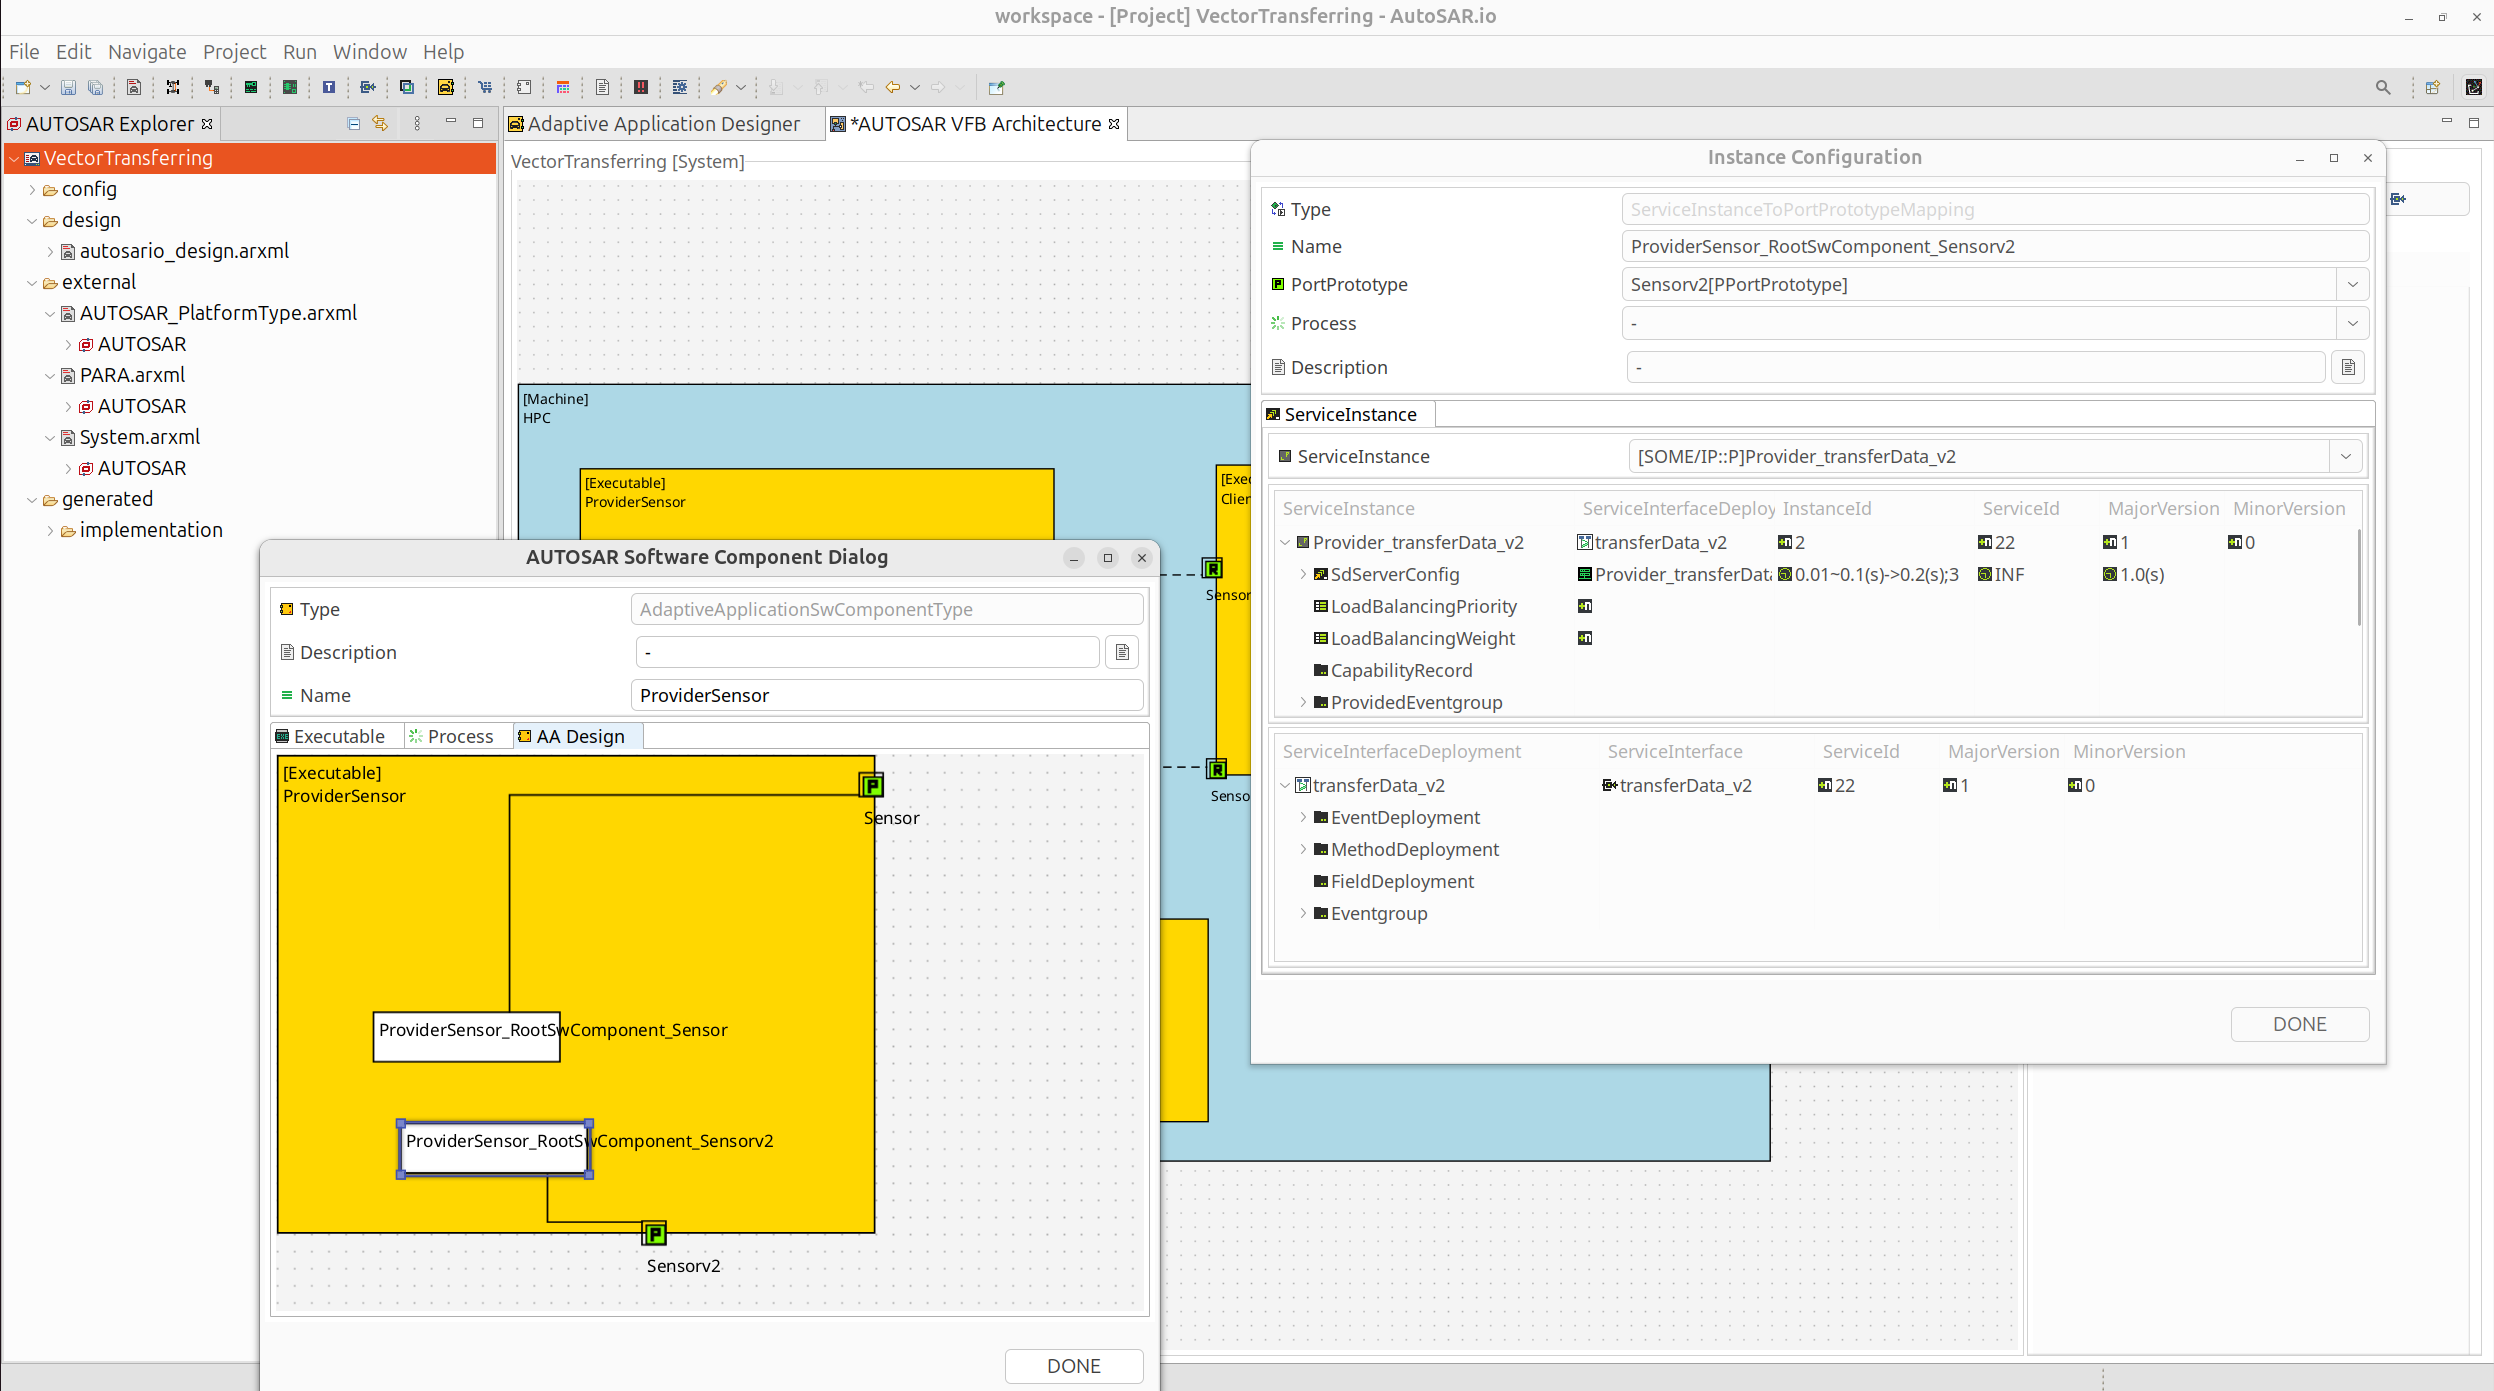
\includegraphics[width=0.75\textwidth]{Images/chap3/image_methodology/applicationDesign/mappingPortProviderEx.png}
    \vspace{0.5cm}
    \caption{Mapping Provider Ports to Service Interface}
    \label{fig:app_mapping_provider_ports}
\end{figure}

Figure~\ref{fig:app_mapping_provider_ports} illustrates the association between the provider executable ports and the previously defined AUTOSAR software component. In this step, the ports of the \texttt{ProviderSensor} executable are mapped to the corresponding port prototypes of the Adaptive Application Software Component that has already been specified in the AUTOSAR model. This configuration establishes a clear link between the executable instance and its software component definition, ensuring that the executable correctly realizes the component’s provided interfaces. As a result, the application implementation becomes consistent with the AUTOSAR architectural model before being bound to concrete service instances and communication middleware.


% Configure Subscriber Executable Properties
\begin{figure}[H]
    \centering
    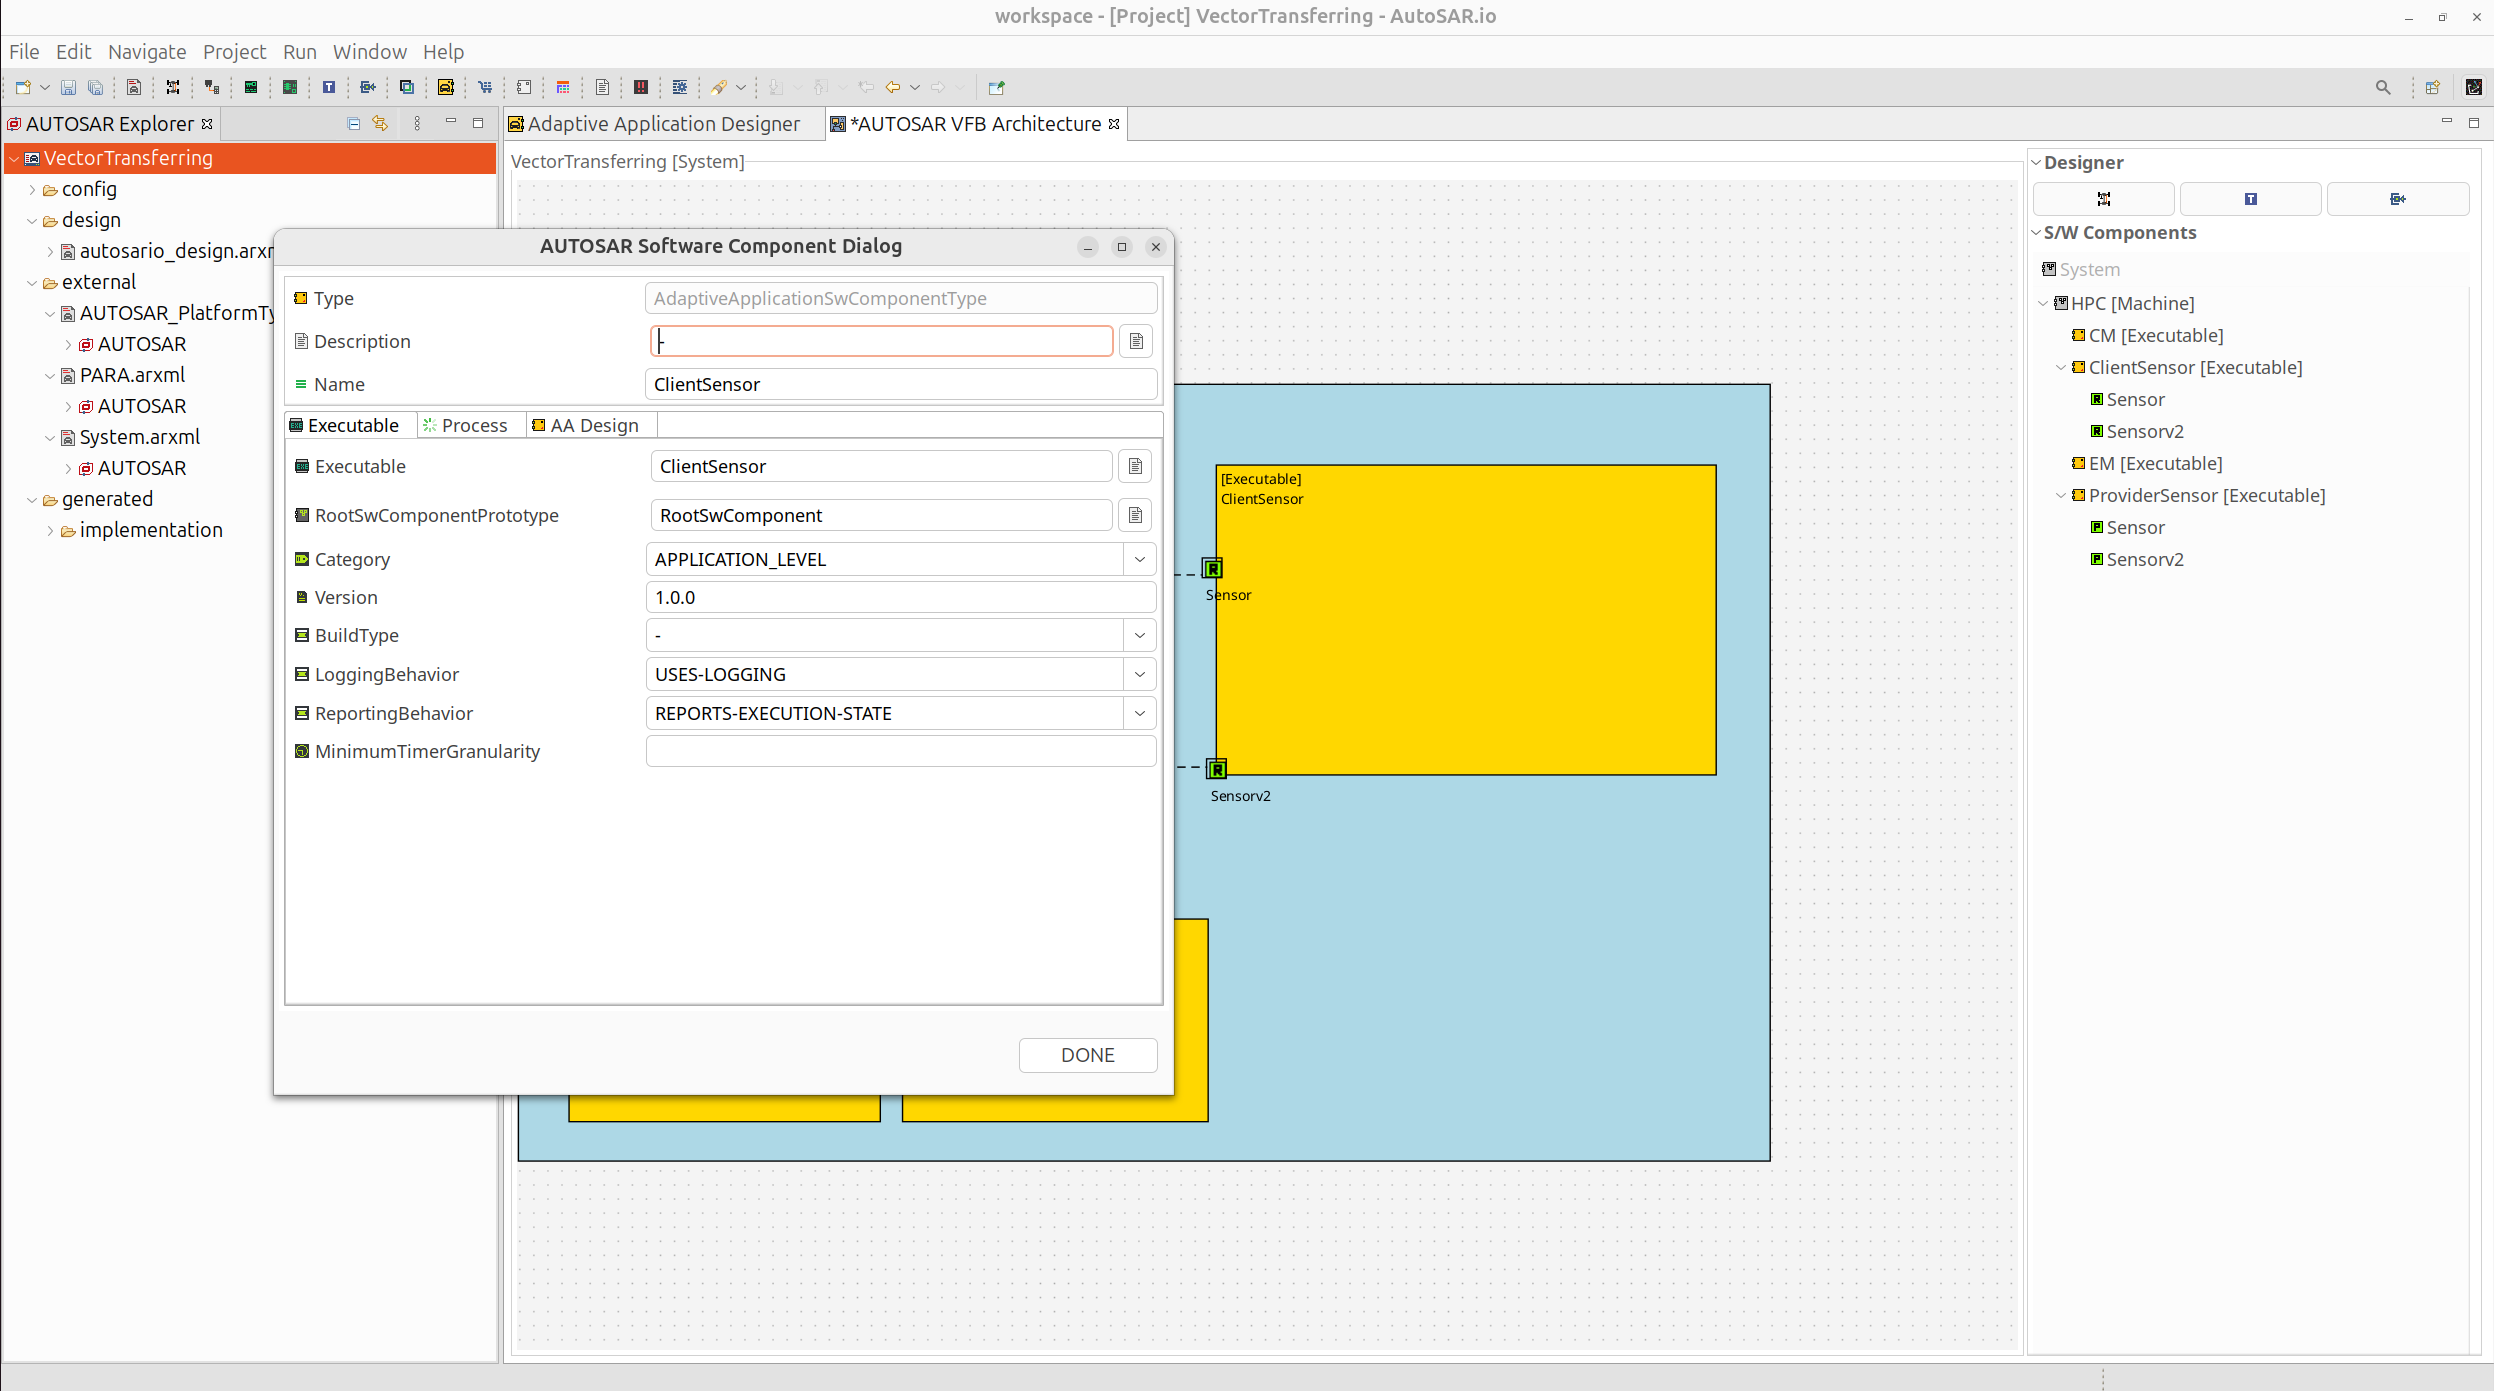
\includegraphics[width=0.75\textwidth]{Images/chap3/image_methodology/applicationDesign/subscriberExProperties.png}
    \vspace{0.5cm}
    \caption{Configuration of Subscriber Executable Properties}
    \label{fig:app_subscriber_executable_properties}
\end{figure}

Figure~\ref{fig:app_subscriber_executable_properties} illustrates the definition of the \texttt{ClientSensor} executable as an adaptive application software component. In this step, the executable is characterized at the application level by specifying its name, version, category, and runtime behavior such as logging and execution state reporting. This configuration formally registers the client application in the AUTOSAR model and establishes it as a runnable entity that can participate in service oriented communication.

% Map Client Ports to Service Interface
\begin{figure}[H]
    \centering
    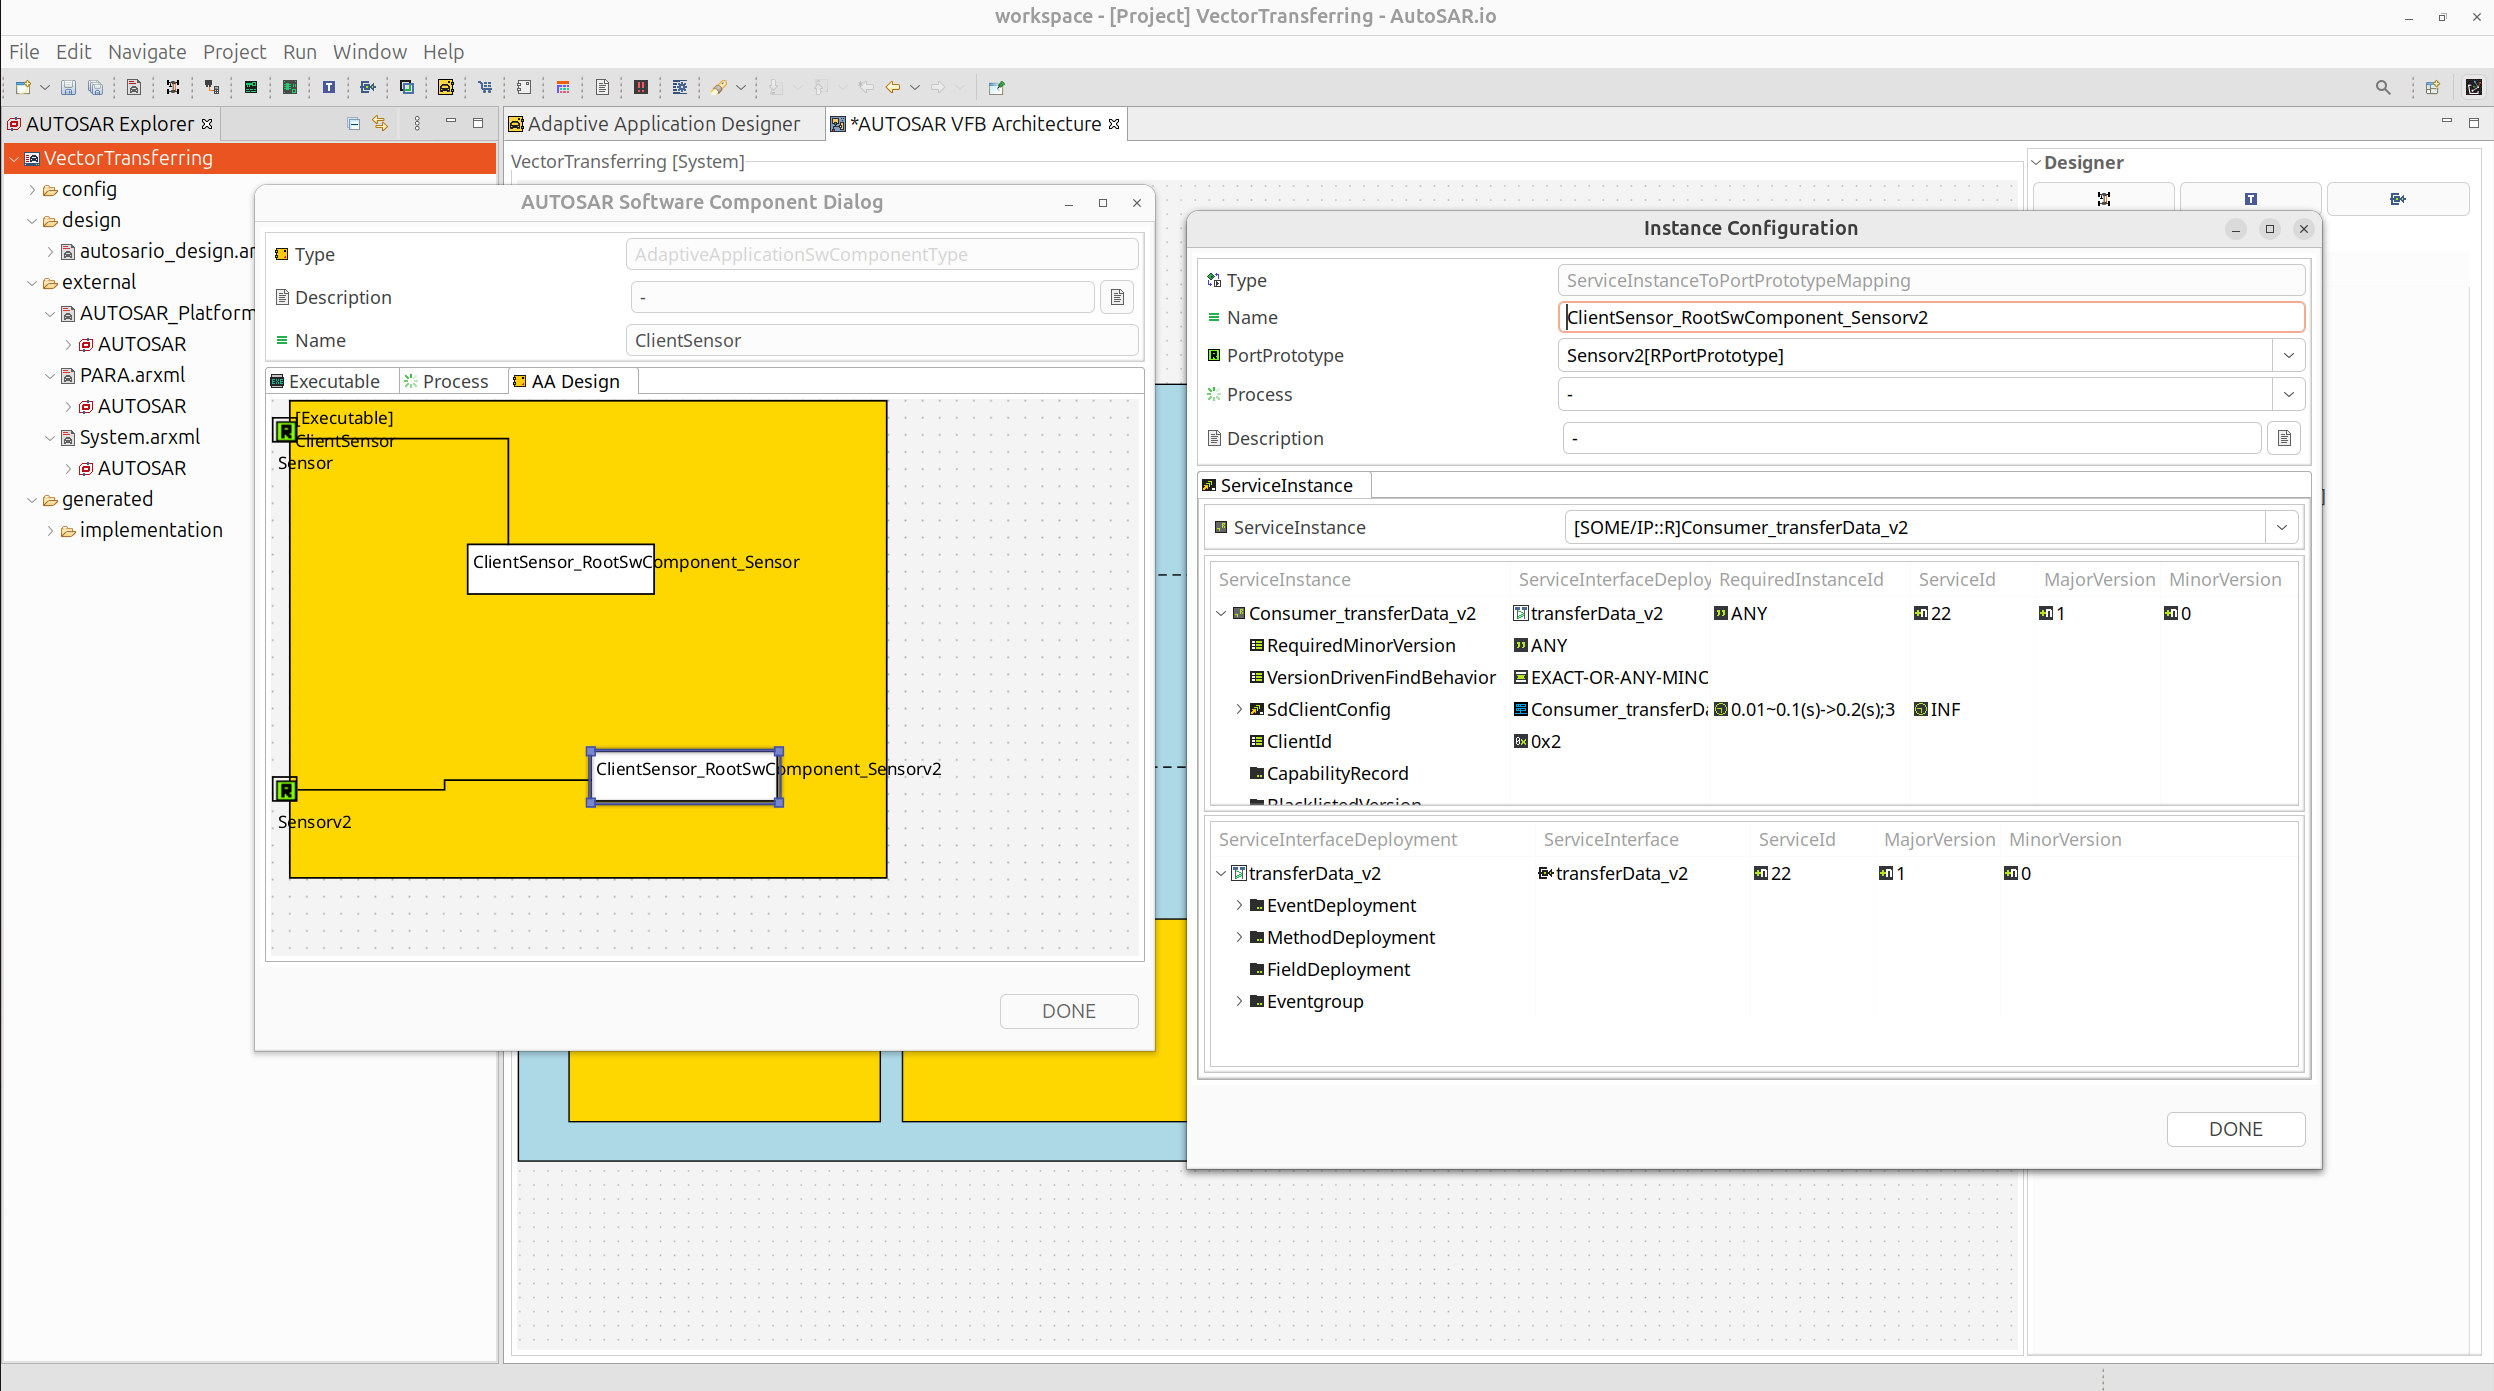
\includegraphics[width=0.75\textwidth]{Images/chap3/image_methodology/applicationDesign/mappingPortClientEx.png}
    \vspace{0.5cm}
    \caption{Mapping Client Ports to Service Interface}
    \label{fig:app_mapping_client_ports}
\end{figure}

As shown in Figure~\ref{fig:app_mapping_client_ports}, the required ports of the \texttt{ClientSensor} software component are then associated with the corresponding port prototypes defined in the AUTOSAR architecture. This association links the client implementation to the abstract interface contracts specified at design time, without directly binding it to network level details. By completing this step, the client executable is structurally aligned with the AUTOSAR software component model, enabling subsequent binding to concrete service instances during service deployment and machine mapping.

% Configure Application Startup Behavior
\begin{figure}[H]
    \centering
    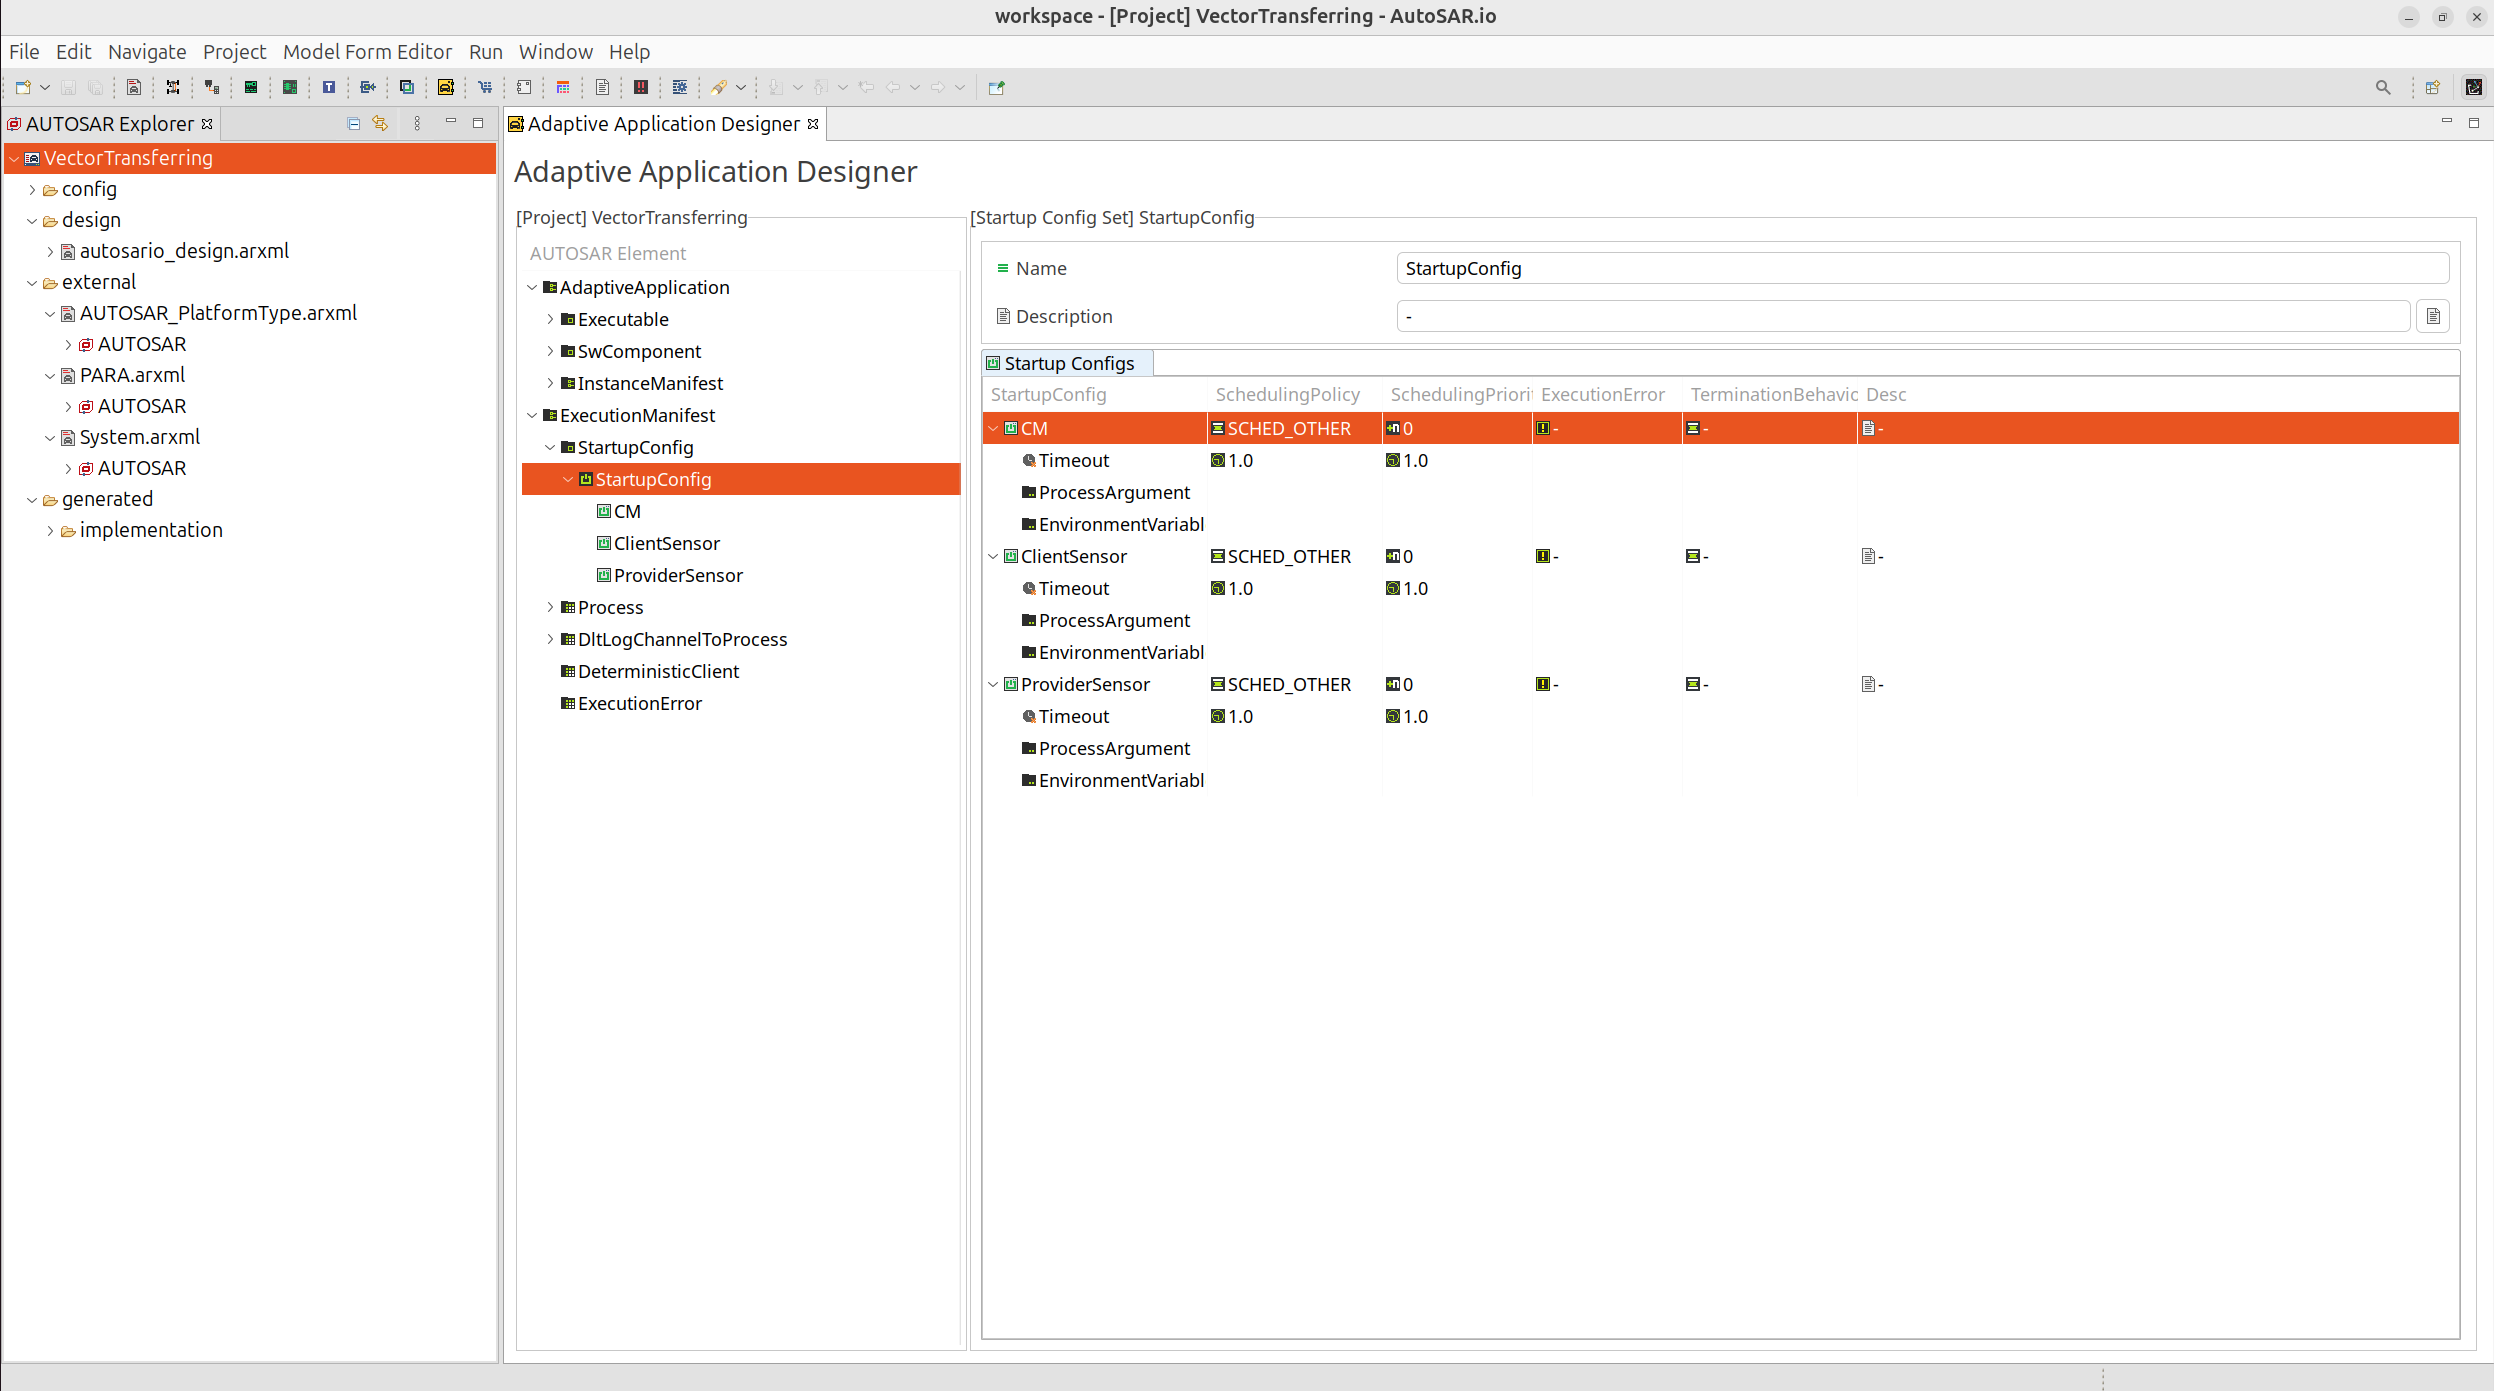
\includegraphics[width=0.75\textwidth]{Images/chap3/image_methodology/applicationDesign/configureStartupConfigure.png}
    \vspace{0.5cm}
    \caption{Configuration of Application Startup Behavior}
    \label{fig:app_startup_configuration}
\end{figure}

Figure~\ref{fig:app_startup_configuration} illustrates the startup configuration set that governs how adaptive application processes are initialized on the target platform. Each process, including \texttt{CM}, \texttt{ClientSensor}, and \texttt{ProviderSensor}, is assigned a scheduling policy and priority, ensuring consistent execution behavior under the POSIX based operating environment. The use of a unified scheduling class allows the platform to manage multiple applications in a predictable manner during system boot.

In addition, the startup configuration defines timeout values and process level parameters that control execution supervision at launch time. By explicitly specifying these attributes, the system ensures that all applications enter a well defined initial state and comply with platform execution constraints. This configuration plays a critical role in coordinating application startup with function group transitions and provides a stable foundation for subsequent runtime interactions.

% Bind DLT Channels to Application Processes
\begin{figure}[H]
    \centering
    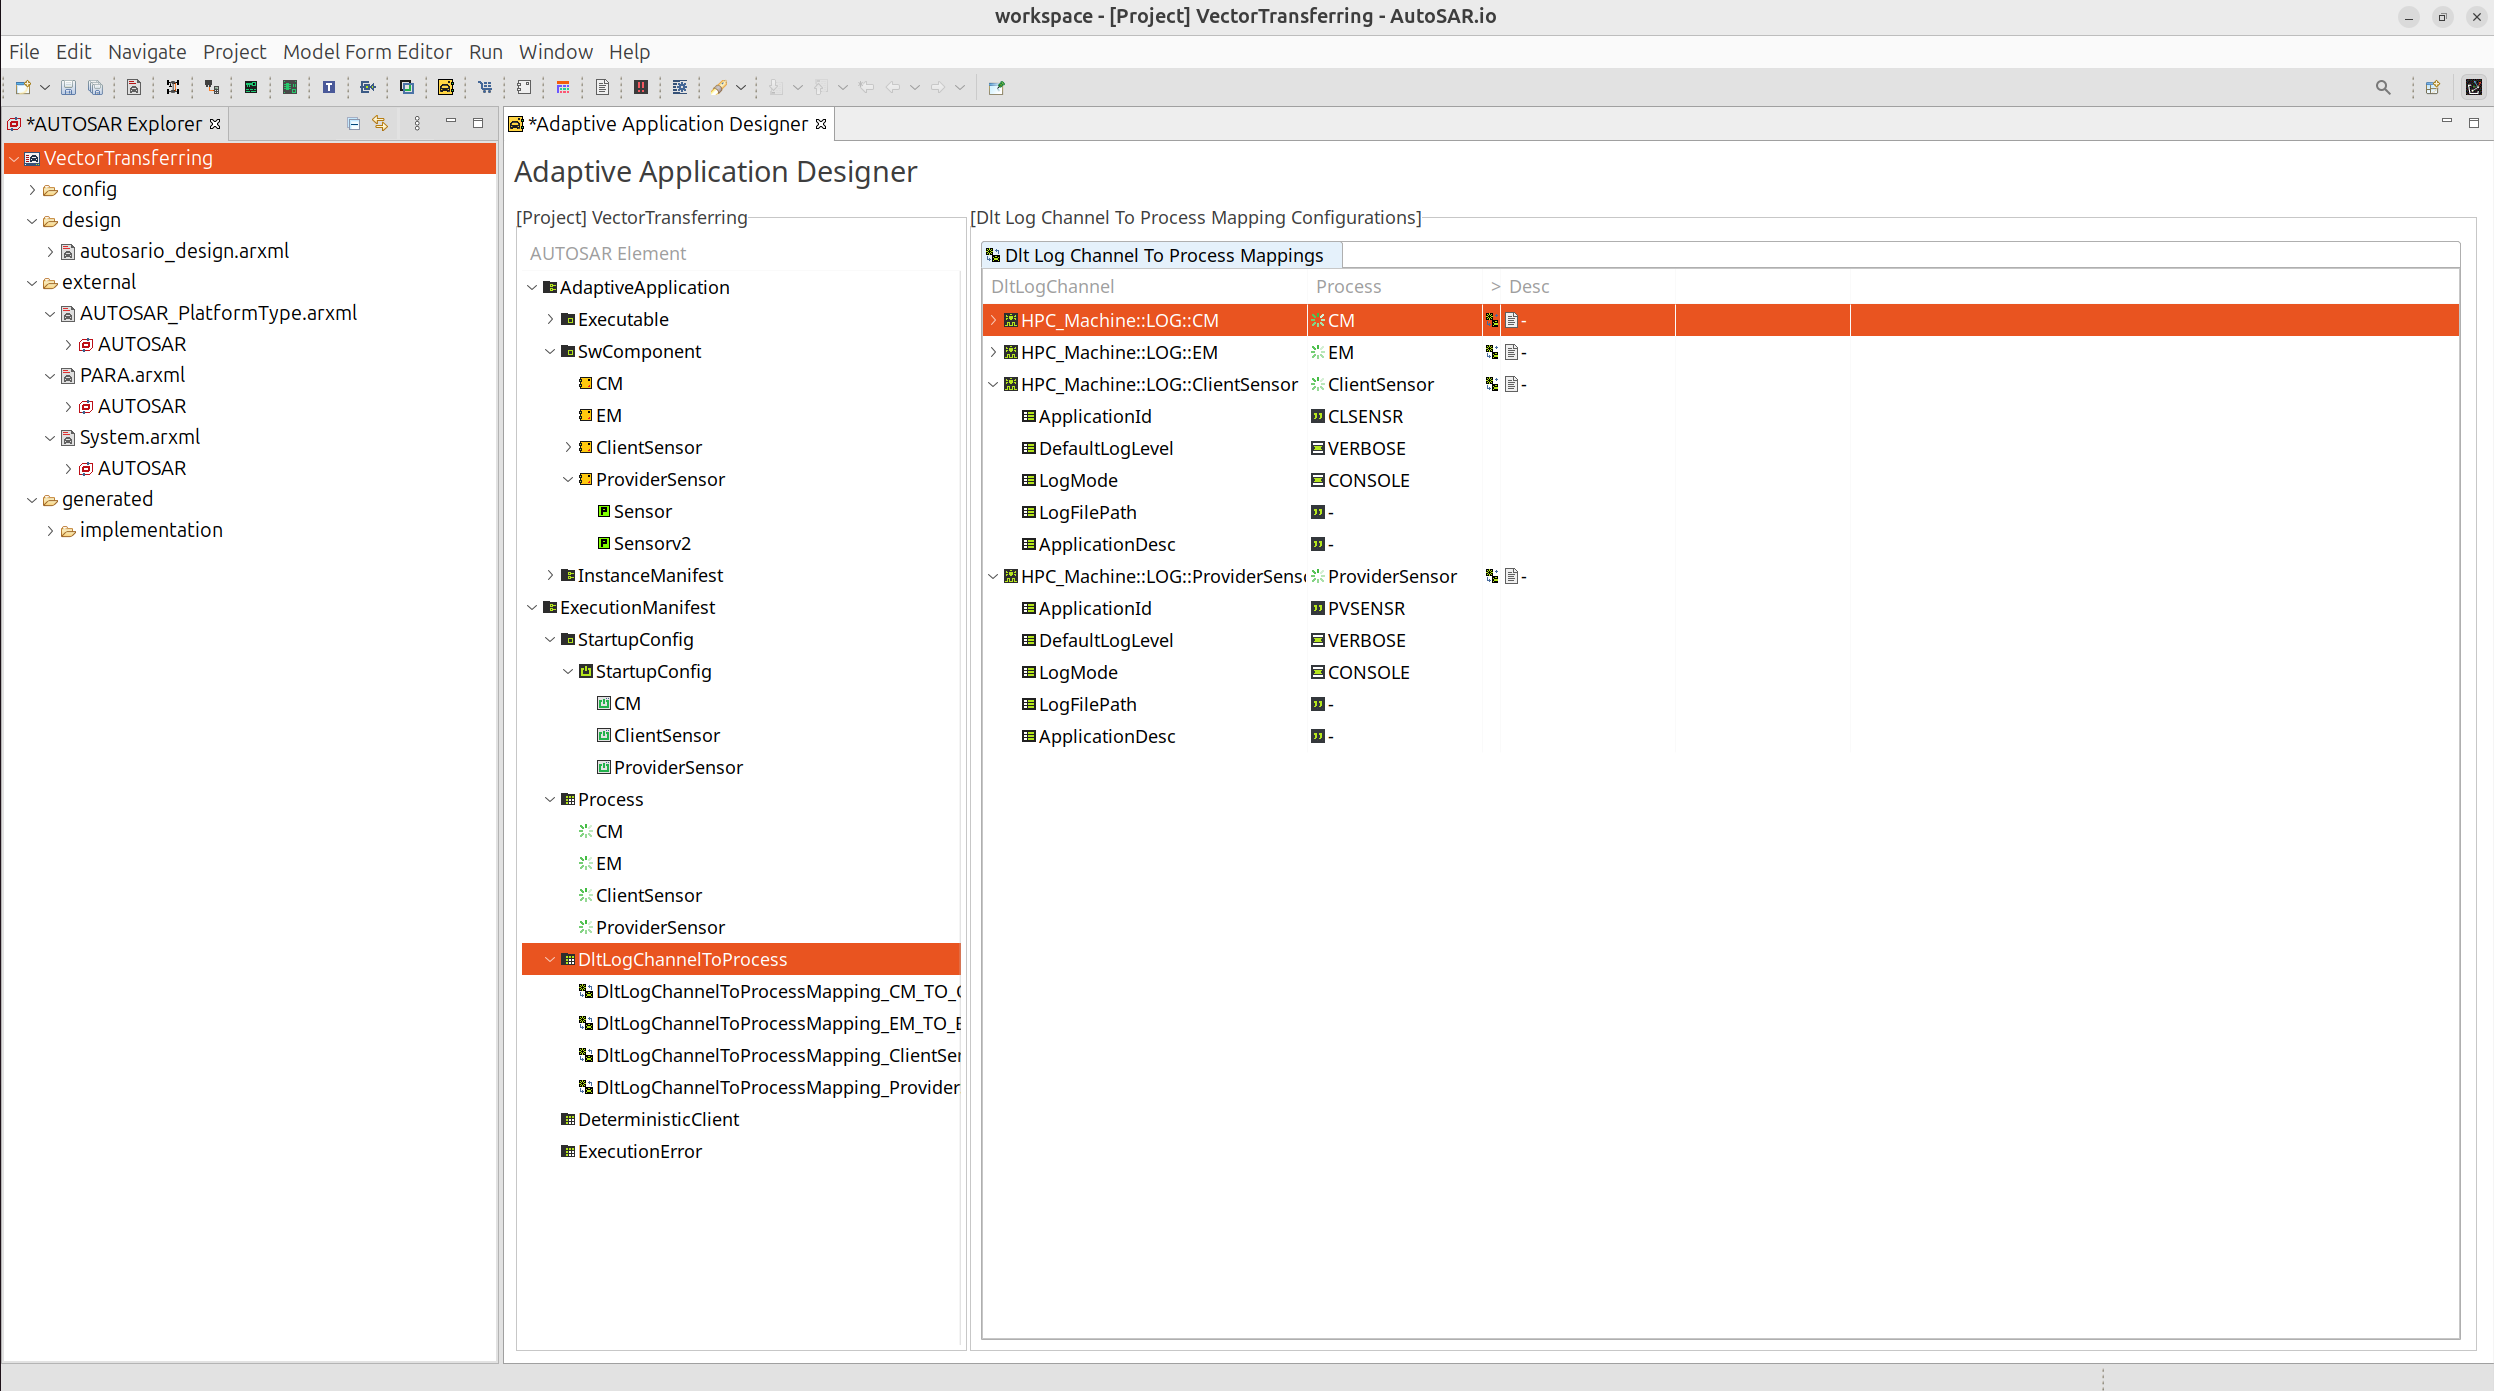
\includegraphics[width=0.75\textwidth]{Images/chap3/image_methodology/applicationDesign/configureDLTChanneltoProcess.png}
    \vspace{0.5cm}
    \caption{Binding Diagnostic Log and Trace Channels to Application Processes}
    \label{fig:app_dlt_process_mapping}
\end{figure}

Figure~\ref{fig:app_dlt_process_mapping} depicts the association between Diagnostic Log and Trace channels and individual application processes. Each process is connected to a specific DLT channel with defined log levels and output modes, enabling consistent monitoring and debugging at runtime. This mapping ensures that diagnostic information is traceable per application, which supports efficient analysis and maintenance in Adaptive AUTOSAR deployments.

% Configure Provider Application Process
\begin{figure}[H]
    \centering
    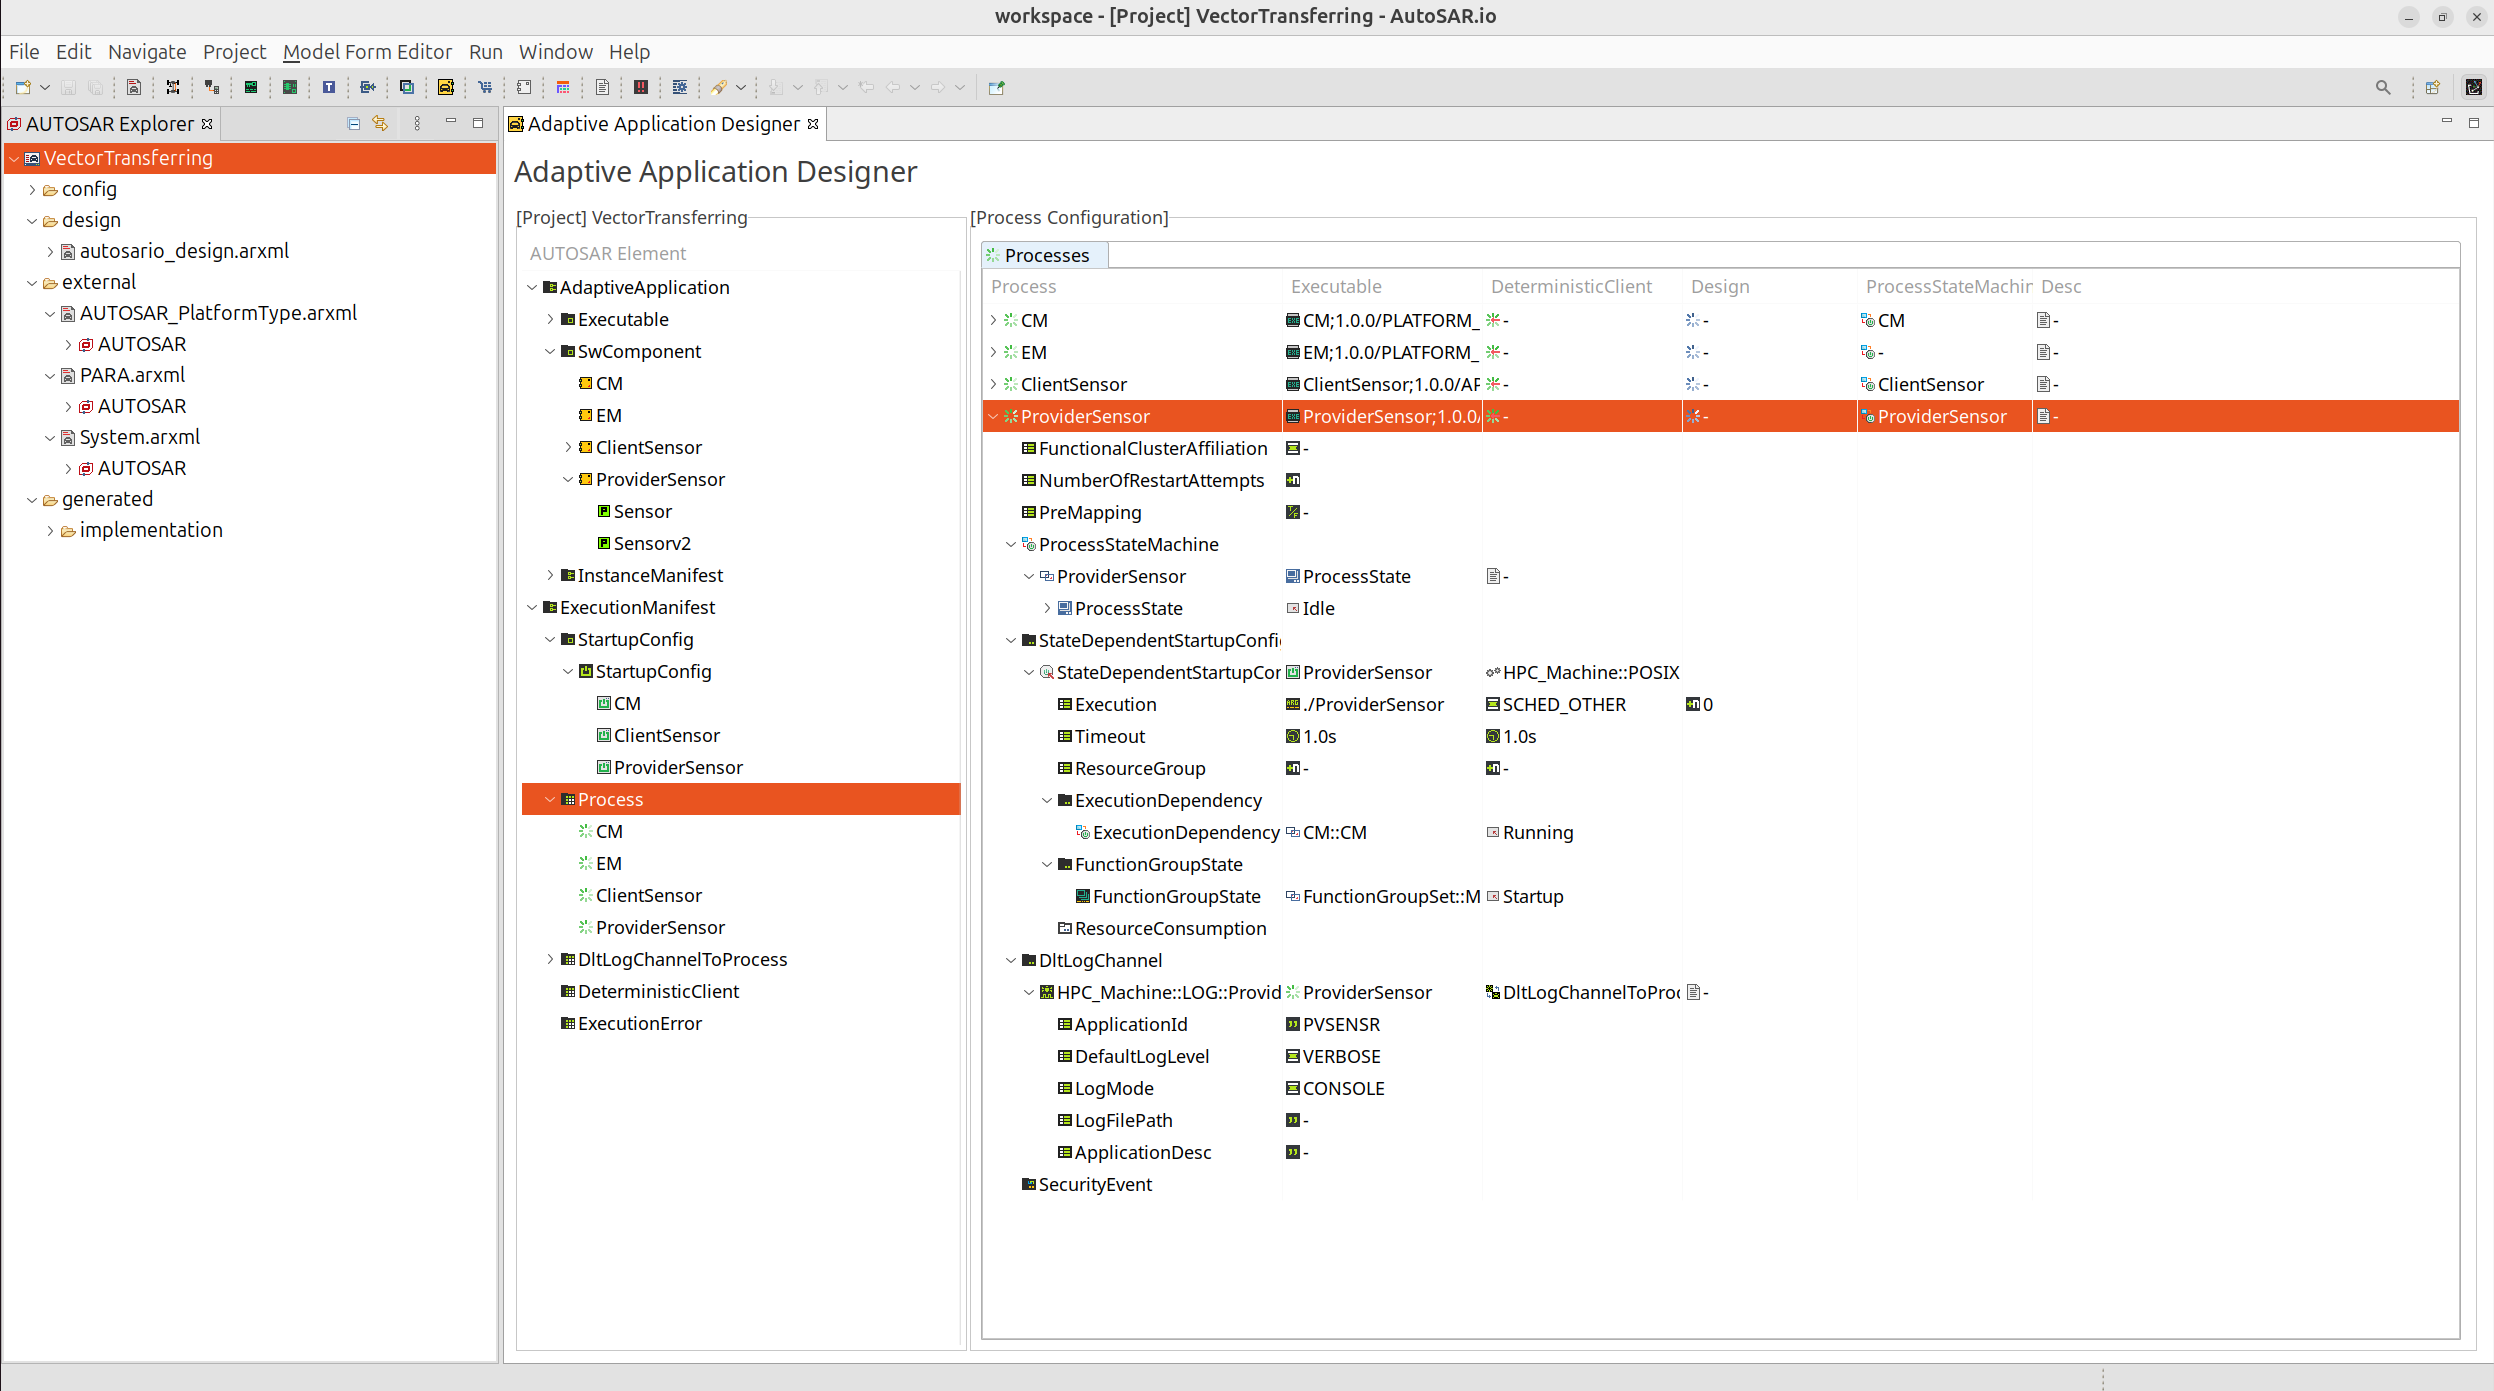
\includegraphics[width=0.75\textwidth]{Images/chap3/image_methodology/applicationDesign/configureProviderProcess.png}
    \vspace{0.5cm}
    \caption{Configuration of Provider Application Process}
    \label{fig:app_provider_process_configuration}
\end{figure}

As illustrated in Figure~\ref{fig:app_provider_process_configuration}, the provider application process is configured by linking the \texttt{ProviderSensor} executable to a dedicated process entity. This step specifies process level attributes such as restart policy, execution dependency, and state machine association, which together describe how the provider behaves during runtime transitions. The configuration clarifies the provider’s role in the execution flow and its dependency on platform level services.

% Configure Client Application Process
\begin{figure}[H]
    \centering
    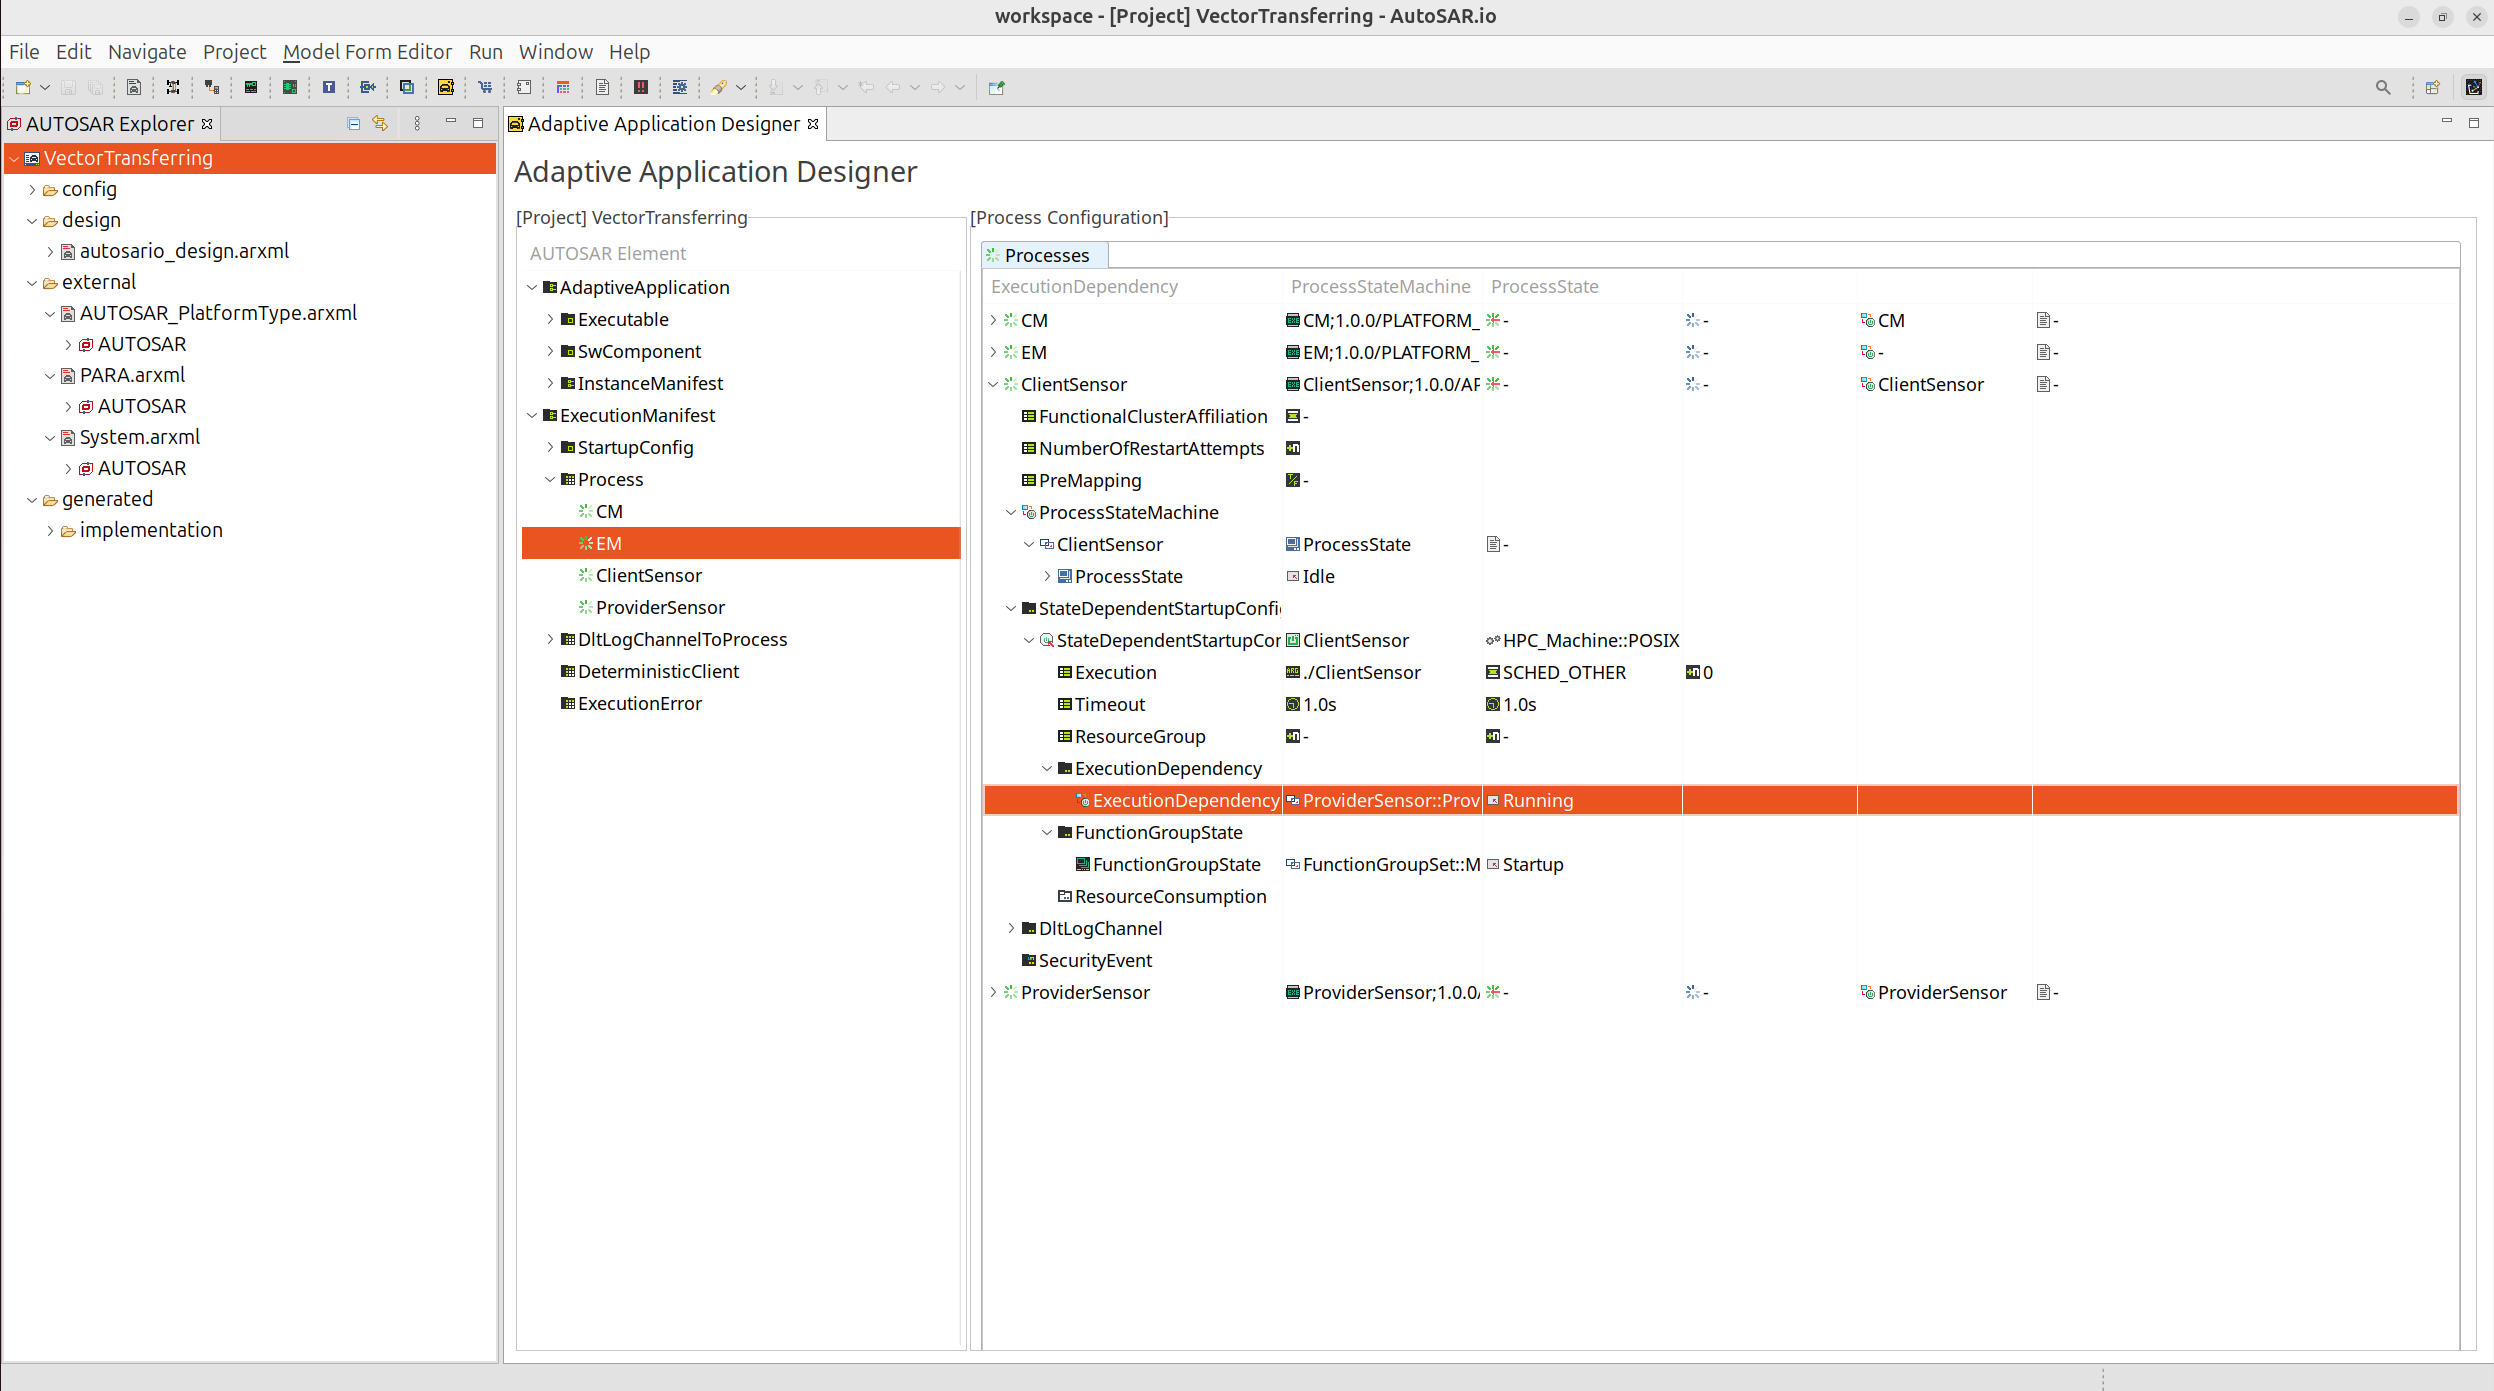
\includegraphics[width=0.75\textwidth]{Images/chap3/image_methodology/applicationDesign/configureClientProcess.png}
    \vspace{0.5cm}
    \caption{Configuration of Client Application Process}
    \label{fig:app_client_process_configuration}
\end{figure}

Figure~\ref{fig:app_client_process_configuration} shows a similar setup for the client application, where the \texttt{ClientSensor} executable is bound to its own process instance. Here, execution states and startup dependencies are defined to ensure that the client is activated only when required conditions are satisfied. This separation at the process level improves modularity and allows independent management of client and provider lifecycles.

% Map Application Processes to Target Machine
\begin{figure}[H]
    \centering
    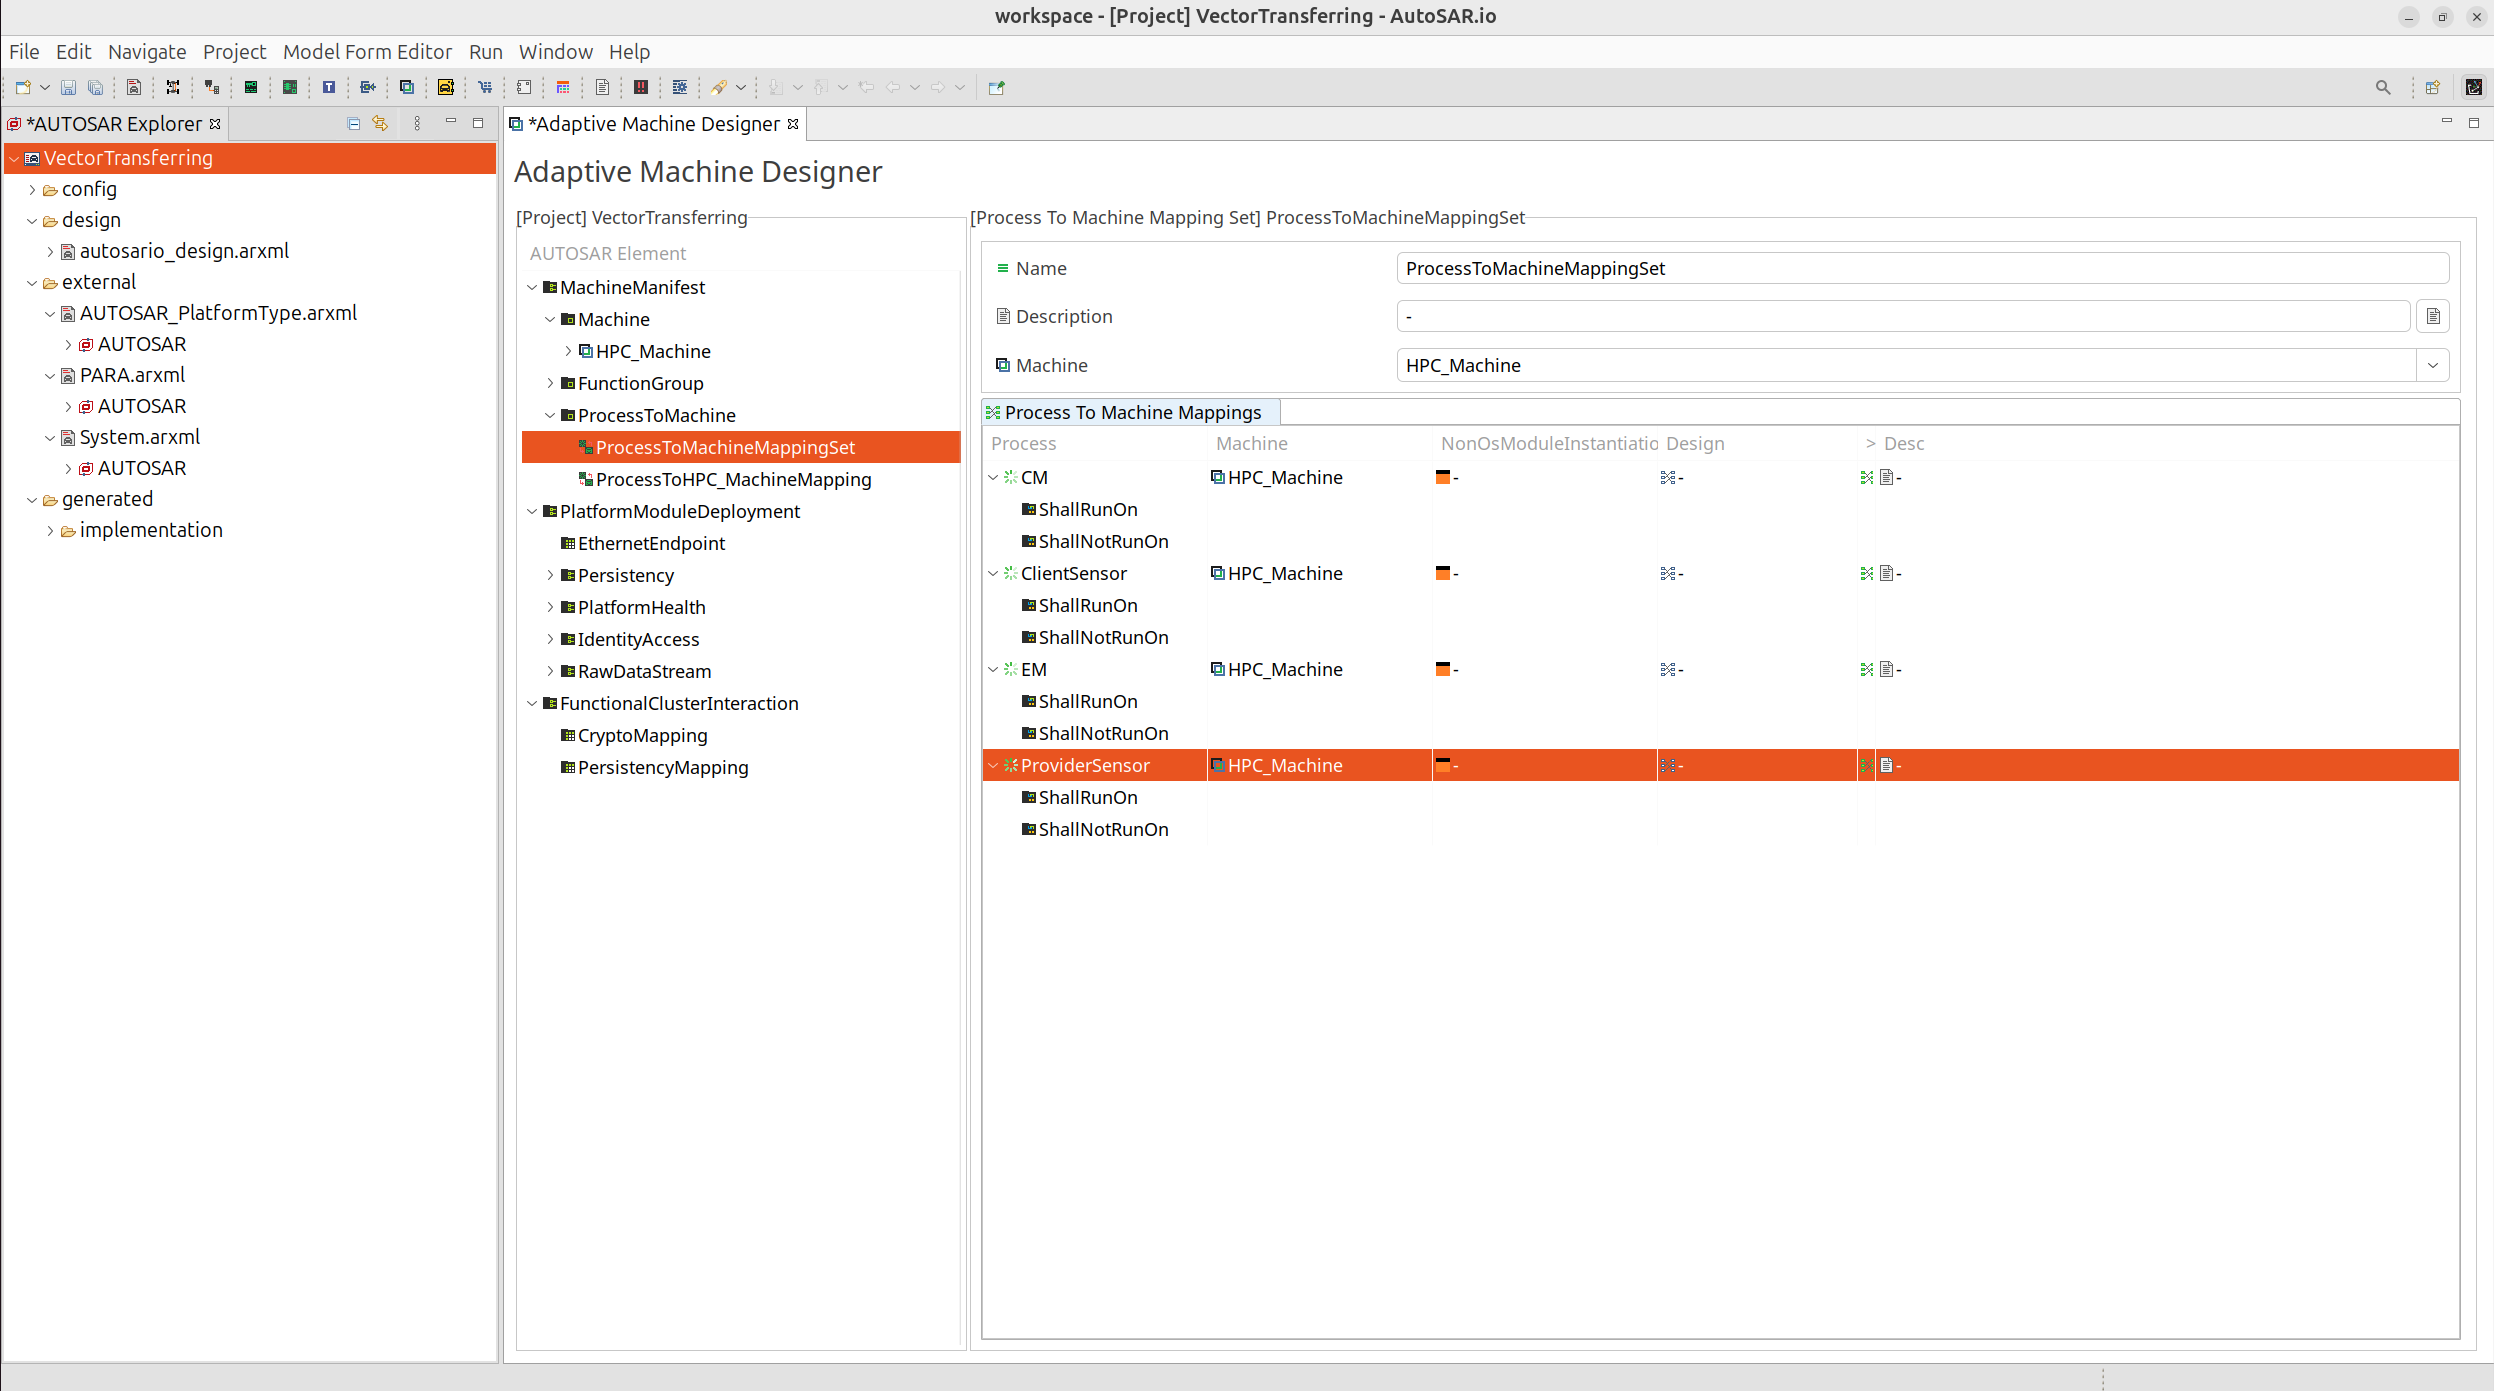
\includegraphics[width=0.75\textwidth]{Images/chap3/image_methodology/applicationDesign/mappingProcesstoMachine.png}
    \vspace{0.5cm}
    \caption{Mapping Application Processes to Target Machine}
    \label{fig:app_process_machine_mapping}
\end{figure}

Finally, Figure~\ref{fig:app_process_machine_mapping} presents the process-to-machine mapping defined in the Adaptive Machine Designer. In this step, all application processes, including \texttt{CM}, \texttt{EM}, \texttt{ClientSensor}, and \texttt{ProviderSensor}, are explicitly assigned to the target \texttt{HPC\_Machine}. This mapping determines the physical execution location of each process and establishes the final deployment relationship between the adaptive applications and the underlying hardware platform.

By consolidating all processes onto a single machine, the configuration ensures a coherent execution environment and simplifies resource management during runtime. This step completes the application deployment workflow by bridging the gap between application-level process definitions and machine-level execution, enabling the Adaptive AUTOSAR runtime to launch and supervise each process according to the previously defined startup, scheduling, and communication configurations.

\subsubsection{Generating Code and Manifest Files}
After completing the configuration steps at the machine, service, and application levels, the Autosar.io tool supports automatic generation of implementation artifacts through the PARA Generator. This generator collects all previously defined models, including Machine Manifests, service definitions, service instances, and application processes, and transforms them into deployable outputs that conform to the Adaptive AUTOSAR specification. By doing so, the tool ensures that the system configuration remains consistent from design time to implementation.

\begin{figure}[H]
    \centering
    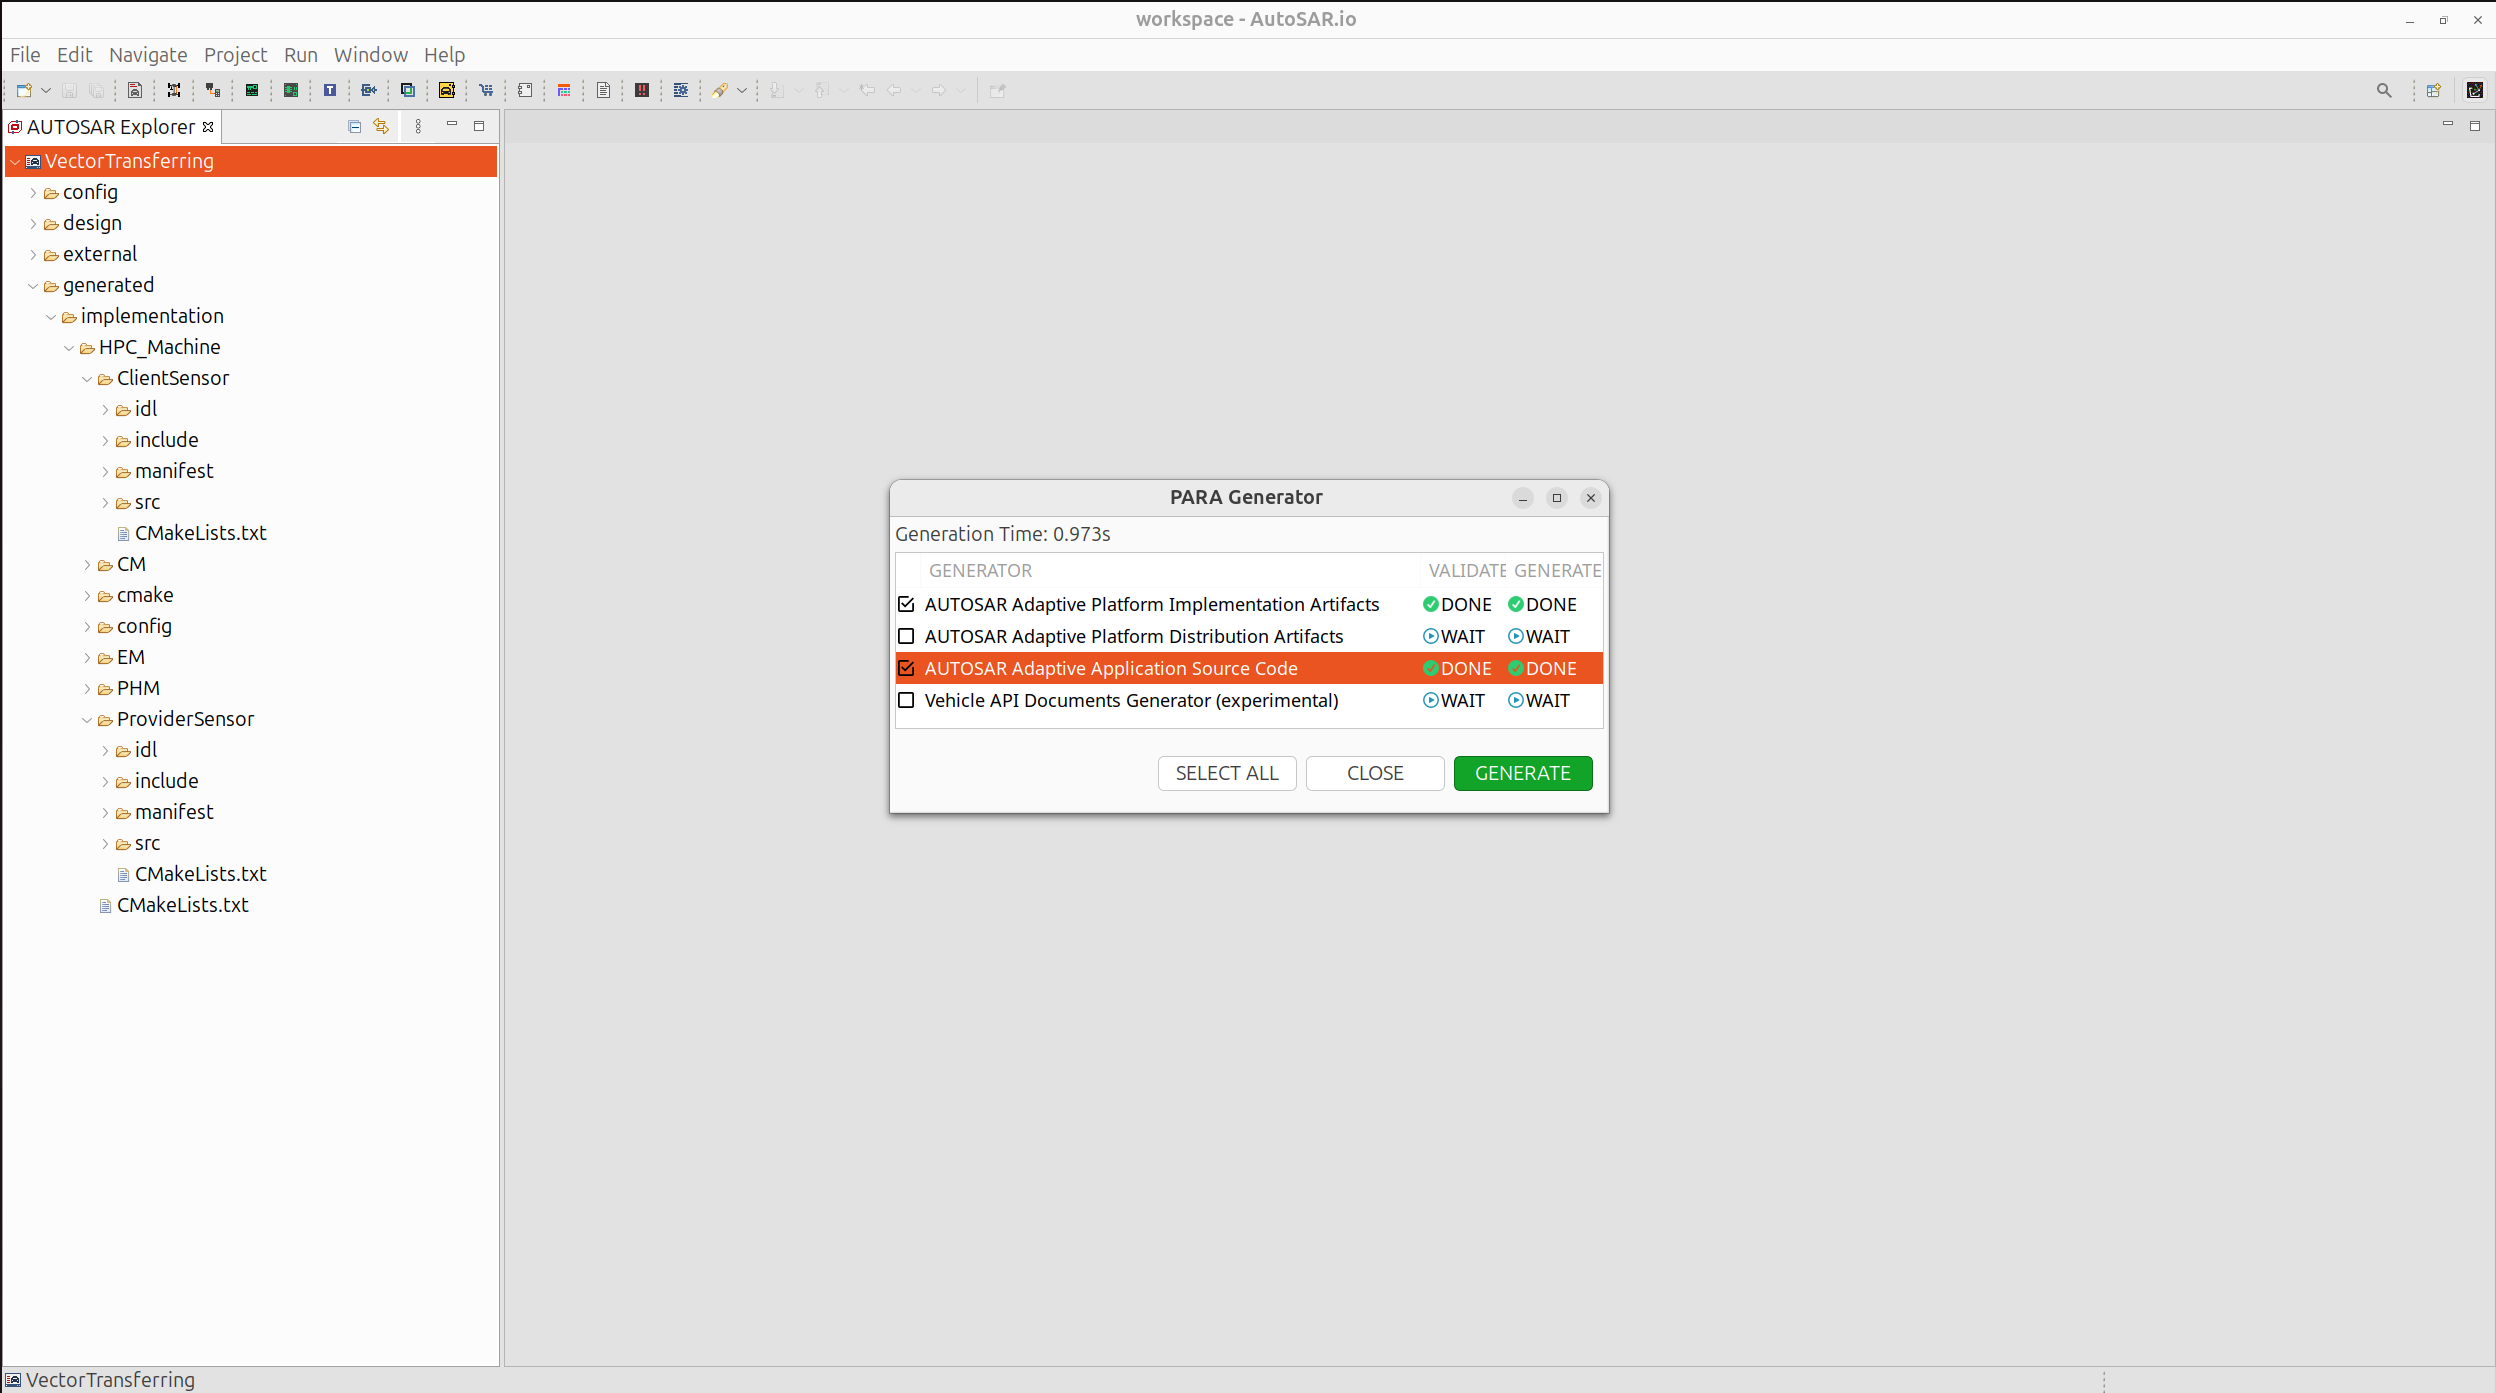
\includegraphics[width=0.75\textwidth]{Images/chap3/generating.png}
    \vspace{0.5cm}
    \caption{Generating Code and ARXML Files}
    \label{fig:code_generation}
\end{figure}

As illustrated in Figure~\ref{fig:code_generation}, the PARA Generator allows users to selectively generate different categories of artifacts, such as Adaptive Application source code, platform configuration files, and manifest descriptions. The generation process produces AUTOSAR compliant ARXML files together with structured C++ source code for each executable. These outputs follow a standardized directory layout, which simplifies subsequent build and integration steps.

Through this automated generation mechanism, Autosar.io bridges the gap between high level system modeling and concrete software artifacts. The generated code and configuration files serve as a reliable foundation for compilation, deployment, and runtime execution. This approach reduces manual errors, improves traceability, and supports a smooth transition from configuration to system integration in the Adaptive AUTOSAR development workflow.

% After establishing the Adaptive AUTOSAR configuration workflow, the system still requires a perception model capable of detecting traffic lights in real time. Therefore, the next subsection shifts from platform configuration to the design and training of the YOLO-MobileNetV4 model. This connection shows how the configured software architecture is supported by an edge-oriented AI component.

% % In this work, we adopt a customized version of the YOLO detection framework by integrating the MobileNetV4 backbone in order to obtain a lightweight yet effective object detection model. The primary motivation behind this design choice is to reduce computational complexity and memory consumption while maintaining reliable detection accuracy. Such requirements are essential for deployment on resource constrained edge devices, including embedded systems, single board computers, and mobile platforms.

% MobileNetV4 is a recently proposed convolutional neural network architecture designed for universal deployment across mobile and edge hardware. It emphasizes efficient feature extraction through improved depthwise separable convolutions, universal inverted bottleneck blocks, and optimized layer scaling strategies. Compared to conventional backbones such as CSPDarknet or standard ResNet variants, MobileNetV4 provides a more balanced trade off between inference speed and representational capability. As a result, it is particularly suitable for real time computer vision tasks where latency, power consumption, and memory footprint are critical constraints.

% \subsection{Backbone Replacement Strategy}

% To integrate MobileNetV4 into the YOLO framework, the default backbone definition is replaced by a customized model configuration file, denoted as \texttt{yolo11-mobilenetv4.yaml}. This configuration follows the standard Ultralytics YOLO model definition format while modifying the backbone section to incorporate MobileNetV4 building blocks. The neck and detection head structures remain largely unchanged in order to preserve compatibility with existing loss functions, anchor settings, and training pipelines.

% The backbone replacement process is performed at the model configuration and module registration level rather than modifying the core training logic. This design choice improves maintainability and simplifies future updates of the YOLO framework. The integration procedure follows a publicly available technical guide that details how MobileNetV4 modules are registered, parsed, and treated as backbone components during model construction\footnote{Guideline for integrating MobileNetV4 into YOLO architectures is available at \url{https://blog.csdn.net/qq_44231797/article/details/147483132}.}. By preserving the feature pyramid structure, multi scale detection capability is maintained despite the lightweight backbone.

% \subsection{Model Initialization and Pretrained Weights}

% To accelerate convergence and improve training stability, the model is initialized using pretrained weights from a lightweight YOLO variant. Specifically, the \texttt{yolo11n.pt} checkpoint is loaded as the initial parameter set. Although the backbone architecture differs from the original YOLO design, partial weight transfer remains beneficial for shared components such as the detection head and certain convolutional layers.

% The Ultralytics YOLO API automatically performs parameter matching where possible and ignores incompatible layers. This mechanism enables the model to leverage prior knowledge while avoiding structural conflicts during initialization. As a result, the training process converges more reliably compared to training from scratch.

% \subsection{Training Configuration}

% The training process is conducted using the Ultralytics YOLO training interface, which provides a flexible and reproducible pipeline for object detection tasks. Dataset information is specified through a YAML configuration file that defines training and validation paths, class labels, and metadata. All input images are resized to a resolution of $320 \times 320$ pixels in order to balance detection accuracy and computational efficiency.

% Stochastic Gradient Descent is selected as the optimization algorithm due to its stable convergence behavior for large scale detection models. Automatic mixed precision is enabled to reduce GPU memory usage and accelerate training while maintaining numerical stability. The model is trained for a total of 400 epochs to ensure sufficient convergence given the modified backbone structure.

% \subsection{Training Script}

% The complete training script used in this study is shown below. This script defines the model configuration, loads pretrained weights, and executes the training process with the selected hyperparameters.

% \begin{lstlisting}[language=Python, caption={YOLO-MobileNetV4 Training Script}]
% # Model configuration file
% model_yaml_path = r"yolo11-mobilenetv4.yaml"

% # Dataset configuration file
% data_yaml_path = r"dataset/data.yaml"

% # Pretrained model
% pre_model_name = "yolo11n.pt"

% import warnings
% warnings.filterwarnings("ignore")

% from ultralytics import YOLO

% if __name__ == "__main__":
%     model = YOLO(model_yaml_path)
%     model.load(pre_model_name)

%     model.train(
%         data=data_yaml_path,
%         cache=False,
%         imgsz=320,
%         epochs=400,
%         workers=8,
%         device="0",
%         optimizer="SGD",
%         amp=True,
%         project="runs/train-yolo-mobilenetv4",
%         name="exp"
%     )
% \end{lstlisting}

\section{YOLO-MobileNetV4 Model}

In this work, we adopt a customized version of the YOLOv26 detection framework by integrating the MobileNetV4 backbone in order to obtain a lightweight yet effective object detection model. The primary motivation behind this design choice is to reduce computational complexity and memory consumption while maintaining reliable detection accuracy. Such requirements are essential for deployment on resource constrained edge devices, including embedded systems, single board computers, and mobile platforms.

\subsection{Integrating MobileNetv4 into YOLO}

Following the our paper in \hyperref[chap:append]{Appendix}, we will continue to integrate MobileNetV4 as the feature extractor for YOLO26 creates a hybrid "YOLO-MNv4" architecture that is theoretically optimal for autonomous driving. On mobile accelerators like the Pixel EdgeTPU, MNv4 is approximately twice as fast as MobileNetV3 for equivalent accuracy due to its high operational intensity. Replacing the standard YOLO26 backbone with MNv4 significantly reduces the floating-point operations (FLOPs) required per inference. This architecture specifically excels in occlusion handling, where the advanced receptive fields of the UIB blocks allow the model to infer the presence of a traffic light even when it is partially obscured by large vehicles, ensuring a robust and reliable perception system.

To adapt the original YOLO26 architecture for edge deployment, several crucial modifications were made (comparing Figure \ref{fig:yolo26_original_arch} to Figure \ref{fig:yolo26_mnv4_arch}). First, the standard heavy CNN backbone was replaced entirely with {MobileNetV4ConvSmall050}. Second, the original 4-head Feature Pyramid Network (P2, P3, P4, P5) was scaled down to a {3-head architecture} (P3, P4, P5) by removing the high-resolution P2 feature extraction path and its corresponding detection head. This reduction dramatically lowers the computational complexity (GFLOPs) and parameter count. Meanwhile, the advanced components of the YOLO26 neck—including the {C3k2} fusion blocks, {SPPF}, {C2PSA} spatial attention, and the {One-to-One Head}-were preserved to maintain state-of-the-art detection logic.

\begin{figure}[htbp]
    \centering
    \resizebox{\textwidth}{!}{
    \begin{tikzpicture}[
        box/.style={rectangle, draw, minimum width=2.4cm, minimum height=0.8cm, text centered, font=\sffamily, rounded corners=2pt},
        arrow/.style={->, >=stealth, thick},
        label/.style={font=\sffamily\scriptsize}
    ]

    % Backbone
    \node[box, fill=blue!10] (input) at (0, 9) {Input (640)};
    \node[box, fill=green!10] (conv1) at (0, 7.5) {Conv P1};
    \node[box, fill=green!10] (p2) at (0, 6) {P2 (C3k2)};
    \node[box, fill=green!10] (p3) at (0, 4) {P3 (C3k2)};
    \node[box, fill=green!10] (p4) at (0, 2) {P4 (C3k2)};
    \node[box, fill=green!10] (p5) at (0, 0) {P5 (C2PSA)};

    \draw[arrow] (input) -- (conv1);
    \draw[arrow] (conv1) -- (p2);
    \draw[arrow] (p2) -- (p3);
    \draw[arrow] (p3) -- (p4);
    \draw[arrow] (p4) -- (p5);

    % SPPF & C2PSA
    \node[box, fill=yellow!10] (sppf) at (3.5, 0) {SPPF};
    \node[box, fill=yellow!10] (c2psa) at (7.0, 0) {C2PSA};
    \draw[arrow] (p5) -- (sppf);
    \draw[arrow] (sppf) -- (c2psa);

    % Neck - Top-down
    \node[box, fill=orange!10] (cat_p4) at (7.0, 2) {Concat};
    \node[box, fill=orange!10] (c3k2_td_p4) at (10.5, 2) {C3k2};
    \draw[arrow] (c2psa) -- node[right, label] {Up} (cat_p4);
    \draw[arrow] (p4) -- (cat_p4);
    \draw[arrow] (cat_p4) -- (c3k2_td_p4);

    \node[box, fill=orange!10] (cat_p3) at (10.5, 4) {Concat};
    \node[box, fill=orange!10] (c3k2_td_p3) at (14.0, 4) {C3k2};
    \draw[arrow] (c3k2_td_p4) -- node[right, label] {Up} (cat_p3);
    \draw[arrow] (p3) -- (cat_p3);
    \draw[arrow] (cat_p3) -- (c3k2_td_p3);

    \node[box, fill=orange!10] (cat_p2) at (14.0, 6) {Concat};
    \node[box, fill=orange!10] (c3k2_td_p2) at (17.5, 6) {C3k2};
    \draw[arrow] (c3k2_td_p3) -- node[right, label] {Up} (cat_p2);
    \draw[arrow] (p2) -- (cat_p2);
    \draw[arrow] (cat_p2) -- (c3k2_td_p2);

    % Neck - Bottom-up
    \node[box, fill=orange!10] (cat_p3_bu) at (17.5, 4) {Concat};
    \node[box, fill=orange!10] (c3k2_bu_p3) at (21.0, 4) {C3k2};
    \draw[arrow] (c3k2_td_p2) -- node[right, label] {Conv s2} (cat_p3_bu);
    \draw[arrow] (c3k2_td_p3) -- (cat_p3_bu);
    \draw[arrow] (cat_p3_bu) -- (c3k2_bu_p3);

    \node[box, fill=orange!10] (cat_p4_bu) at (21.0, 2) {Concat};
    \node[box, fill=orange!10] (c3k2_bu_p4) at (24.5, 2) {C3k2};
    \draw[arrow] (c3k2_bu_p3) -- node[right, label] {Conv s2} (cat_p4_bu);
    \draw[arrow] (c3k2_td_p4) -- (cat_p4_bu);
    \draw[arrow] (cat_p4_bu) -- (c3k2_bu_p4);

    \node[box, fill=orange!10] (cat_p5_bu) at (24.5, 0) {Concat};
    \node[box, fill=orange!10] (c3k2_bu_p5) at (28.0, 0) {C3k2};
    \draw[arrow] (c3k2_bu_p4) -- node[right, label] {Conv s2} (cat_p5_bu);
    \draw[arrow] (c2psa) -- (cat_p5_bu);
    \draw[arrow] (cat_p5_bu) -- (c3k2_bu_p5);

    % Detectors
    \node[box, fill=red!10] (head2) at (31.5, 6) {Detect P2};
    \node[box, fill=red!10] (head3) at (31.5, 4) {Detect P3};
    \node[box, fill=red!10] (head4) at (31.5, 2) {Detect P4};
    \node[box, fill=red!10] (head5) at (31.5, 0) {Detect P5};
    
    \node[box, fill=purple!10, align=center, minimum height=1.6cm] (detect) at (35.0, 3) {One-to-One\\Head};

    \draw[arrow] (c3k2_td_p2) -- (head2);
    \draw[arrow] (c3k2_bu_p3) -- (head3);
    \draw[arrow] (c3k2_bu_p4) -- (head4);
    \draw[arrow] (c3k2_bu_p5) -- (head5);
    
    \draw[arrow] (head2) -| (detect);
    \draw[arrow] (head3) -| (detect);
    \draw[arrow] (head4) -| (detect);
    \draw[arrow] (head5) -| (detect);

    \end{tikzpicture}
    }
    \vspace{0.5cm}
    \caption{Architecture of the original YOLO26-p2 model with 4-head detection mechanism (P2/P3/P4/P5 outputs) for standard object detection tasks. Channel widths scale with the chosen model variant (n/s/m/l/x).}
    \label{fig:yolo26_original_arch}
\end{figure}

\begin{figure}[htbp]
    \centering
    \resizebox{\textwidth}{!}{
    \begin{tikzpicture}[
        box/.style={rectangle, draw, minimum width=2.4cm, minimum height=0.8cm, text centered, font=\sffamily, rounded corners=2pt},
        arrow/.style={->, >=stealth, thick},
        label/.style={font=\sffamily\scriptsize}
    ]

    % X coordinates:
    % 0.0: Backbone
    % 3.5: SPPF
    % 7.0: C2PSA, cat1
    % 10.5: c3k2_1, cat2
    % 14.0: c3k2_2, cat3
    % 17.5: c3k2_3, cat4
    % 21.0: c3k2_4
    % 24.5: Detectors
    % 28.0: Head

    % Backbone
    \node[box, fill=blue!10] (input) at (0, 8) {Input (416)};
    \node[box, fill=green!10] (mnv4) at (0, 6) {MobileNetV4};
    \node[box, fill=green!10] (p3) at (0, 4) {P3 (32c)};
    \node[box, fill=green!10] (p4) at (0, 2) {P4 (48c)};
    \node[box, fill=green!10] (p5) at (0, 0) {P5 (640c)};

    \draw[arrow] (input) -- (mnv4);
    \draw[arrow] (mnv4) -- (p3);
    \draw[arrow] (p3) -- (p4);
    \draw[arrow] (p4) -- (p5);

    % SPPF & C2PSA
    \node[box, fill=yellow!10] (sppf) at (3.5, 0) {SPPF (256c)};
    \node[box, fill=yellow!10] (c2psa) at (7.0, 0) {C2PSA (256c)};
    \draw[arrow] (p5) -- (sppf);
    \draw[arrow] (sppf) -- (c2psa);

    % Neck - Top-down
    \node[box, fill=orange!10] (cat1) at (7.0, 2) {Concat};
    \node[box, fill=orange!10] (c3k2_1) at (10.5, 2) {C3k2 (128c)};
    \draw[arrow] (c2psa) -- node[right, label] {Up} (cat1);
    \draw[arrow] (p4) -- (cat1);
    \draw[arrow] (cat1) -- (c3k2_1);

    \node[box, fill=orange!10] (cat2) at (10.5, 4) {Concat};
    \node[box, fill=orange!10] (c3k2_2) at (14.0, 4) {C3k2 (64c)};
    \draw[arrow] (c3k2_1) -- node[right, label] {Up} (cat2);
    \draw[arrow] (p3) -- (cat2);
    \draw[arrow] (cat2) -- (c3k2_2);

    % Neck - Bottom-up
    \node[box, fill=orange!10] (cat3) at (14.0, 2) {Concat};
    \node[box, fill=orange!10] (c3k2_3) at (17.5, 2) {C3k2 (128c)};
    \draw[arrow] (c3k2_2) -- node[right, label] {Conv s2} (cat3);
    \draw[arrow] (c3k2_1) -- (cat3);
    \draw[arrow] (cat3) -- (c3k2_3);

    \node[box, fill=orange!10] (cat4) at (17.5, 0) {Concat};
    \node[box, fill=orange!10] (c3k2_4) at (21.0, 0) {C3k2 (256c)};
    \draw[arrow] (c3k2_3) -- node[right, label] {Conv s2} (cat4);
    \draw[arrow] (c2psa) -- (cat4);
    \draw[arrow] (cat4) -- (c3k2_4);

    % Detectors
    \node[box, fill=red!10] (head1) at (24.5, 4) {Detect P3};
    \node[box, fill=red!10] (head2) at (24.5, 2) {Detect P4};
    \node[box, fill=red!10] (head3) at (24.5, 0) {Detect P5};
    
    \node[box, fill=purple!10, align=center] (detect) at (28.0, 2) {One-to-One\\Head};

    \draw[arrow] (c3k2_2) -- (head1);
    \draw[arrow] (c3k2_3) -- (head2);
    \draw[arrow] (c3k2_4) -- (head3);
    
    \draw[arrow] (head1) -| (detect);
    \draw[arrow] (head2) -- (detect);
    \draw[arrow] (head3) -| (detect);

    \end{tikzpicture}
    }
    \vspace{0.5cm} % Add some space before caption to prevent overlap
    \caption{Architecture of the YOLO26 model with MobileNetV4ConvSmall050 backbone, dual-head mechanism, and NMS-free end-to-end detection, tailored for $416\times416$ resolution.}
    \label{fig:yolo26_mnv4_arch}
\end{figure}

% \subsection{Training Hyperparameters}

% The training process is conducted using the Ultralytics YOLO training API, which provides a reproducible and configurable pipeline for object detection tasks. The dataset is specified through a YAML configuration file (\texttt{TrafficLightV5.v9i.yolo26/data.yaml}) that defines training and validation image paths, class labels, and metadata. To bootstrap training, pretrained weights from \texttt{yolo26n.pt} are loaded via partial weight transfer; compatible layers (primarily in the neck and head) inherit learned parameters, while the MobileNetV4 backbone is initialised from scratch. The \texttt{end2end=True} flag activates the One-to-One head for NMS-free training. Table~\ref{tab:hyperparams} summarises the key hyperparameters.

% \begin{table}[htbp]
% \centering
% \caption{Selected training hyperparameters for the YOLO26-MobileNetV4 model.}
% \label{tab:hyperparams}
% \renewcommand{\arraystretch}{1.15}
% \begin{tabular}{l l l}
% \hline
% \textbf{Parameter} & \textbf{Value} & \textbf{Rationale} \\
% \hline
% \texttt{imgsz} & $416 \times 416$ & Balance between spatial resolution and edge inference speed \\
% \texttt{epochs} & 100 & Sufficient convergence for the modified backbone \\
% \texttt{batch} & 16 & Fits within GPU memory with MobileNetV4 backbone \\
% \texttt{patience} & 100 & Disable early stopping; run full cosine LR cycle \\
% \texttt{optimizer} & auto (SGD) & Stable convergence for detection models \\
% \texttt{lr0} & 0.005 & Slightly elevated initial LR for unfrozen backbone \\
% \texttt{lrf} & 0.01 & Final LR ratio: $\text{lr}_{\text{final}} = 0.01 \times \text{lr}_0$ \\
% \texttt{cos\_lr} & True & Cosine annealing for smooth convergence in late epochs \\
% \texttt{warmup\_epochs} & 3.0 & Gradual LR ramp-up to stabilise early gradients \\
% \texttt{amp} & True & Mixed-precision training for memory efficiency \\
% \texttt{freeze} & None & All layers trainable; no backbone freezing \\
% \texttt{close\_mosaic} & 10 & Disable mosaic augmentation in the last 10 epochs \\
% \hline
% \texttt{box} & 7.5 & Bounding box regression loss weight \\
% \texttt{cls} & 0.5 & Classification loss weight \\
% \texttt{dfl} & 1.5 & DFL loss weight (set but unused since YOLO26 removes DFL) \\
% \hline
% \end{tabular}
% \end{table}

% \subsubsection{Optimiser and Learning Rate Schedule}
% The optimiser is set to \texttt{auto}, which defaults to Stochastic Gradient Descent (SGD) with Nesterov momentum ($\mu = 0.937$) and weight decay ($\lambda = 5 \times 10^{-4}$). The initial learning rate is set to $\text{lr}_0 = 0.005$, slightly higher than the default $0.01$ to compensate for the unfrozen MobileNetV4 backbone requiring larger gradient steps to adapt to the traffic light domain. A cosine annealing schedule (\texttt{cos\_lr=True}) smoothly decays the learning rate to $\text{lr}_0 \times \text{lrf} = 5 \times 10^{-5}$ over the full 100 epochs, ensuring fine-grained convergence in the later stages of training without the abrupt transitions of step-decay schedules.

% \subsubsection{No Backbone Freezing}
% Unlike transfer learning approaches that freeze the backbone during initial epochs, this configuration leaves all layers trainable (\texttt{freeze=None}). Since the MobileNetV4ConvSmall050 backbone differs fundamentally from the original YOLO26 backbone, the pretrained weights only partially transfer. Freezing would prevent the new backbone from learning domain-specific features such as the distinctive shapes and colours of Vietnamese traffic light signal heads and arrow indicators.

% \subsubsection{Image Augmentation Strategy}
% The augmentation pipeline is carefully tuned for the traffic light detection domain:

% \begin{itemize}
%     \item \textbf{Colour jitter}: Hue shift is minimal (\texttt{hsv\_h}$=0.015$) to preserve the critical red/green/yellow colour semantics of traffic signals. Saturation (\texttt{hsv\_s}$=0.7$) and brightness (\texttt{hsv\_v}$=0.4$) augmentation are moderate to improve robustness under varying lighting conditions without corrupting colour-dependent class distinctions.
%     \item \textbf{Geometric transforms}: Translation (\texttt{translate}$=0.1$) and scale (\texttt{scale}$=0.5$) are enabled to simulate varying camera distances and positions. Rotation (\texttt{degrees}$=0.0$) and shear (\texttt{shear}$=0.0$) are disabled since traffic lights are always vertically oriented.
%     \item \textbf{Flipping disabled}: Both horizontal (\texttt{fliplr}$=0.0$) and vertical (\texttt{flipud}$=0.0$) flips are strictly disabled. Horizontal flipping would reverse the direction of left/right arrow turn signals, creating incorrect training labels.
%     \item \textbf{Mosaic}: Set to 0.5 probability to composite multiple training images into one frame, improving the model's ability to detect small, densely packed objects such as timer digit clusters. Mosaic is automatically disabled in the last 10 epochs (\texttt{close\_mosaic}$=10$) so the model fine-tunes on unmodified real images.
%     \item \textbf{MixUp and CopyPaste}: Both disabled (\texttt{mixup}$=0.0$, \texttt{copy\_paste}$=0.0$) to avoid blending signals from different classes, which could confuse the network on colour-critical traffic light states.
% \end{itemize}


\subsection{Dataset and Hyper parameters}
\label{sub:datasetYolo}
A well-prepared dataset and carefully tuned hyperparameters are essential for successfully training the modified YOLO-MobileNetV4 model. This section details the dataset used for traffic light detection, including its composition and pre-processing steps, before explaining the specific training configurations and augmentation strategies applied to ensure robust performance.

\subsubsection{Dataset Composition and Pre-processing}
The model is trained and evaluated on the \texttt{TrafficLightV5.v9i.yolo26} dataset, which comprises a total of 4,867 images. The dataset is annotated in the YOLO format and structured to detect four classes: \texttt{left}, \texttt{right}, \texttt{straight}, and \texttt{timer}. The images are partitioned into three splits: 4,260 images for training, 406 for validation, and 201 for testing. Prior to model ingestion, offline pre-processing and augmentations were applied via Roboflow. The pre-processing includes auto-orientation and resizing to $416 \times 416$ pixels (fit with black edges). The offline augmentation strategy generates three versions of each source image by applying random rotation ($-5^\circ$ to $+5^\circ$), random shear ($-2^\circ$ to $+2^\circ$), exposure adjustments ($\pm 10\%$), and salt-and-pepper noise ($0.1\%$ of pixels).

\subsubsection{Training Configuration}
The training process is conducted using the Ultralytics YOLO training API, which provides a reproducible and configurable pipeline for object detection tasks. The dataset is specified through a YAML configuration file (\texttt{TrafficLightV5.v9i.yolo26/data.yaml}) that defines training and validation image paths, class labels, and metadata. To bootstrap training, pretrained weights from \texttt{yolo26n.pt} are loaded via partial weight transfer; compatible layers (primarily in the neck and head) inherit learned parameters, while the MobileNetV4 backbone is initialised from scratch. The \texttt{end2end=True} flag activates the One-to-One head for NMS-free training. Table~\ref{tab:hyperparams} summarises the key hyperparameters.

\begin{table}[htbp]
\centering
\caption{Selected training hyperparameters for the YOLO26-MobileNetV4 model.}
\label{tab:hyperparams}
\renewcommand{\arraystretch}{1.15}
\begin{tabular}{l l l}
\hline
\textbf{Parameter} & \textbf{Value} & \textbf{Rationale} \\
\hline
\texttt{imgsz} & $416 \times 416$ & Balance between spatial resolution and edge inference speed \\
\texttt{epochs} & 100 & Sufficient convergence for the modified backbone \\
\texttt{batch} & 16 & Fits within GPU memory with MobileNetV4 backbone \\
\texttt{patience} & 100 & Disable early stopping; run full cosine LR cycle \\
\texttt{optimizer} & auto (SGD) & Stable convergence for detection models \\
\texttt{lr0} & 0.005 & Slightly elevated initial LR for unfrozen backbone \\
\texttt{lrf} & 0.01 & Final LR ratio: $\text{lr}_{\text{final}} = 0.01 \times \text{lr}_0$ \\
\texttt{cos\_lr} & True & Cosine annealing for smooth convergence in late epochs \\
\texttt{warmup\_epochs} & 3.0 & Gradual LR ramp-up to stabilise early gradients \\
\texttt{amp} & True & Mixed-precision training for memory efficiency \\
\texttt{freeze} & None & All layers trainable; no backbone freezing \\
\texttt{close\_mosaic} & 10 & Disable mosaic augmentation in the last 10 epochs \\
\hline
\texttt{box} & 7.5 & Bounding box regression loss weight \\
\texttt{cls} & 0.5 & Classification loss weight \\
\texttt{dfl} & 1.5 & DFL loss weight (set but unused since YOLO26 removes DFL) \\
\hline
\end{tabular}
\end{table}

\subsubsection{Optimiser and Learning Rate Schedule}
The optimiser is set to \texttt{auto}, which defaults to Stochastic Gradient Descent (SGD) with Nesterov momentum ($\mu = 0.937$) and weight decay ($\lambda = 5 \times 10^{-4}$). The initial learning rate is set to $\text{lr}_0 = 0.005$, slightly higher than the default $0.01$ to compensate for the unfrozen MobileNetV4 backbone requiring larger gradient steps to adapt to the traffic light domain. A cosine annealing schedule (\texttt{cos\_lr=True}) smoothly decays the learning rate to $\text{lr}_0 \times \text{lrf} = 5 \times 10^{-5}$ over the full 100 epochs, ensuring fine-grained convergence in the later stages of training without the abrupt transitions of step-decay schedules.

\subsubsection{No Backbone Freezing}
Unlike transfer learning approaches that freeze the backbone during initial epochs, this configuration leaves all layers trainable (\texttt{freeze=None}). Since the MobileNetV4ConvSmall050 backbone differs fundamentally from the original YOLO26 backbone, the pretrained weights only partially transfer. Freezing would prevent the new backbone from learning domain-specific features such as the distinctive shapes and colours of Vietnamese traffic light signal heads and arrow indicators.

\subsubsection{Image Augmentation Strategy}
The augmentation pipeline is carefully tuned for the traffic light detection domain:

\begin{itemize}
    \item \textbf{Colour jitter}: Hue shift is minimal (\texttt{hsv\_h}$=0.015$) to preserve the critical red/green/yellow colour semantics of traffic signals. Saturation (\texttt{hsv\_s}$=0.7$) and brightness (\texttt{hsv\_v}$=0.4$) augmentation are moderate to improve robustness under varying lighting conditions without corrupting colour-dependent class distinctions.
    \item \textbf{Geometric transforms}: Translation (\texttt{translate}$=0.1$) and scale (\texttt{scale}$=0.5$) are enabled to simulate varying camera distances and positions. Rotation (\texttt{degrees}$=0.0$) and shear (\texttt{shear}$=0.0$) are disabled since traffic lights are always vertically oriented.
    \item \textbf{Flipping disabled}: Both horizontal (\texttt{fliplr}$=0.0$) and vertical (\texttt{flipud}$=0.0$) flips are strictly disabled. Horizontal flipping would reverse the direction of left/right arrow turn signals, creating incorrect training labels.
    \item \textbf{Mosaic}: Set to 0.5 probability to composite multiple training images into one frame, improving the model's ability to detect small, densely packed objects such as timer digit clusters. Mosaic is automatically disabled in the last 10 epochs (\texttt{close\_mosaic}$=10$) so the model fine-tunes on unmodified real images.
    \item \textbf{MixUp and CopyPaste}: Both disabled (\texttt{mixup}$=0.0$, \texttt{copy\_paste}$=0.0$) to avoid blending signals from different classes, which could confuse the network on colour-critical traffic light states.
\end{itemize}

\subsection{Exporting to TFLite with INT8 Quantisation}

To deploy the trained YOLO26-MobileNetV4 model on edge devices such as the Raspberry Pi 5, the model must be converted from its native PyTorch format to TensorFlow Lite (TFLite). The Ultralytics export pipeline automates this multi-stage conversion: PyTorch $\to$ ONNX $\to$ TensorFlow SavedModel $\to$ TFLite. The export is performed with the following configuration:

\begin{lstlisting}[language=Python, caption={YOLO26-MobileNetV4 TFLite export script.}, label={lst:export}]
from ultralytics import YOLO

model = YOLO("runs/train/yolo26_mobilenetv4_custom/weights/best.pt")

model.export(
    format="tflite",
    imgsz=416,
    int8=True,
    data='TrafficLightV5.v9i.yolo26/data.yaml',
    batch=1,
    end2end=True,
)
\end{lstlisting}

\subsubsection{INT8 Post-Training Quantisation.}
Full-integer quantisation maps all floating-point weights and activations to 8-bit integers, reducing the model size by approximately $4\times$ and enabling the use of integer-only arithmetic on ARM NEON SIMD units. The quantisation scheme represents each tensor value $x$ as:

\begin{equation}
\label{eq:quant}
  x_q = \text{round}\!\left(\frac{x}{s}\right) + z,
  \qquad
  s = \frac{x_{\max} - x_{\min}}{255},
  \qquad
  z = \text{round}\!\left(-\frac{x_{\min}}{s}\right),
\end{equation}

where $s$ is the per-tensor scale factor and $z$ is the zero-point, both determined during the calibration phase. To compute these statistics, a representative subset of training images from the dataset specified by the \texttt{data} parameter is fed through the network. This calibration step records the dynamic range of each activation tensor, enabling the converter to choose optimal scale and zero-point values that minimise quantisation error across the domain-specific input distribution.

\subsubsection{End-to-End Export}
The \texttt{end2end=True} flag preserves the One-to-One detection head in the exported model graph, ensuring that the TFLite model produces final detection results directly without requiring an external NMS post-processing step. This is critical for edge deployment because it eliminates the need for custom NMS operators that may not be supported by all TFLite delegates, and guarantees deterministic output tensor shapes $(1, 300, 6)$ regardless of input content.

\subsubsection{Deployment Considerations}
The resulting INT8 TFLite model is deployed via the LiteRT (formerly TensorFlow Lite) interpreter on the target device. With \texttt{batch=1} and \texttt{imgsz=416}, the model is optimised for single-frame, real-time inference. The quantised flatbuffer file is significantly smaller than the original float32 model, fitting within the L2 cache of the Cortex-A76 cores on the Raspberry Pi 5, which minimises memory access latency during inference.

% \subsubsection{Accuracy}

% Based on the quantitative trends observed in Figures~\ref{fig:yolomobilenetv4} and~\ref{fig:code_generation}, the original YOLOv11n model achieves slightly higher detection accuracy compared to the YOLOv11n-MobileNetV4 variant. Specifically, the original model attains marginally better precision, recall, and mean Average Precision across the evaluated metrics.

% From the mAP@50 curves, the original YOLOv11n model achieves an improvement of approximately 10--15\% compared to the MobileNetV4-based model. A similar performance gap is observed for mAP@50--95, where the original architecture demonstrates around 10--15\% higher accuracy under stricter localization thresholds. These differences indicate that the original backbone provides stronger feature representation capability, particularly for precise object localization.

% Nevertheless, the overall performance gap remains relatively small. The YOLO-MobileNetV4 model preserves more than 95\% of the detection accuracy achieved by the original YOLOv11n while significantly reducing model complexity. Precision and recall curves further confirm that both models exhibit comparable convergence behavior, with the MobileNetV4 variant showing slightly lower but stable accuracy throughout training.

% These results highlight a clear trade off between accuracy and efficiency. While the original YOLOv11n model offers slightly superior detection accuracy, the YOLO-MobileNetV4 configuration provides a more balanced solution by achieving competitive accuracy with reduced computational cost. This balance makes the MobileNetV4-based model particularly suitable for deployment in edge oriented and resource constrained environments where efficiency is a primary concern.


% \begin{figure}[H]
%     \centering
%     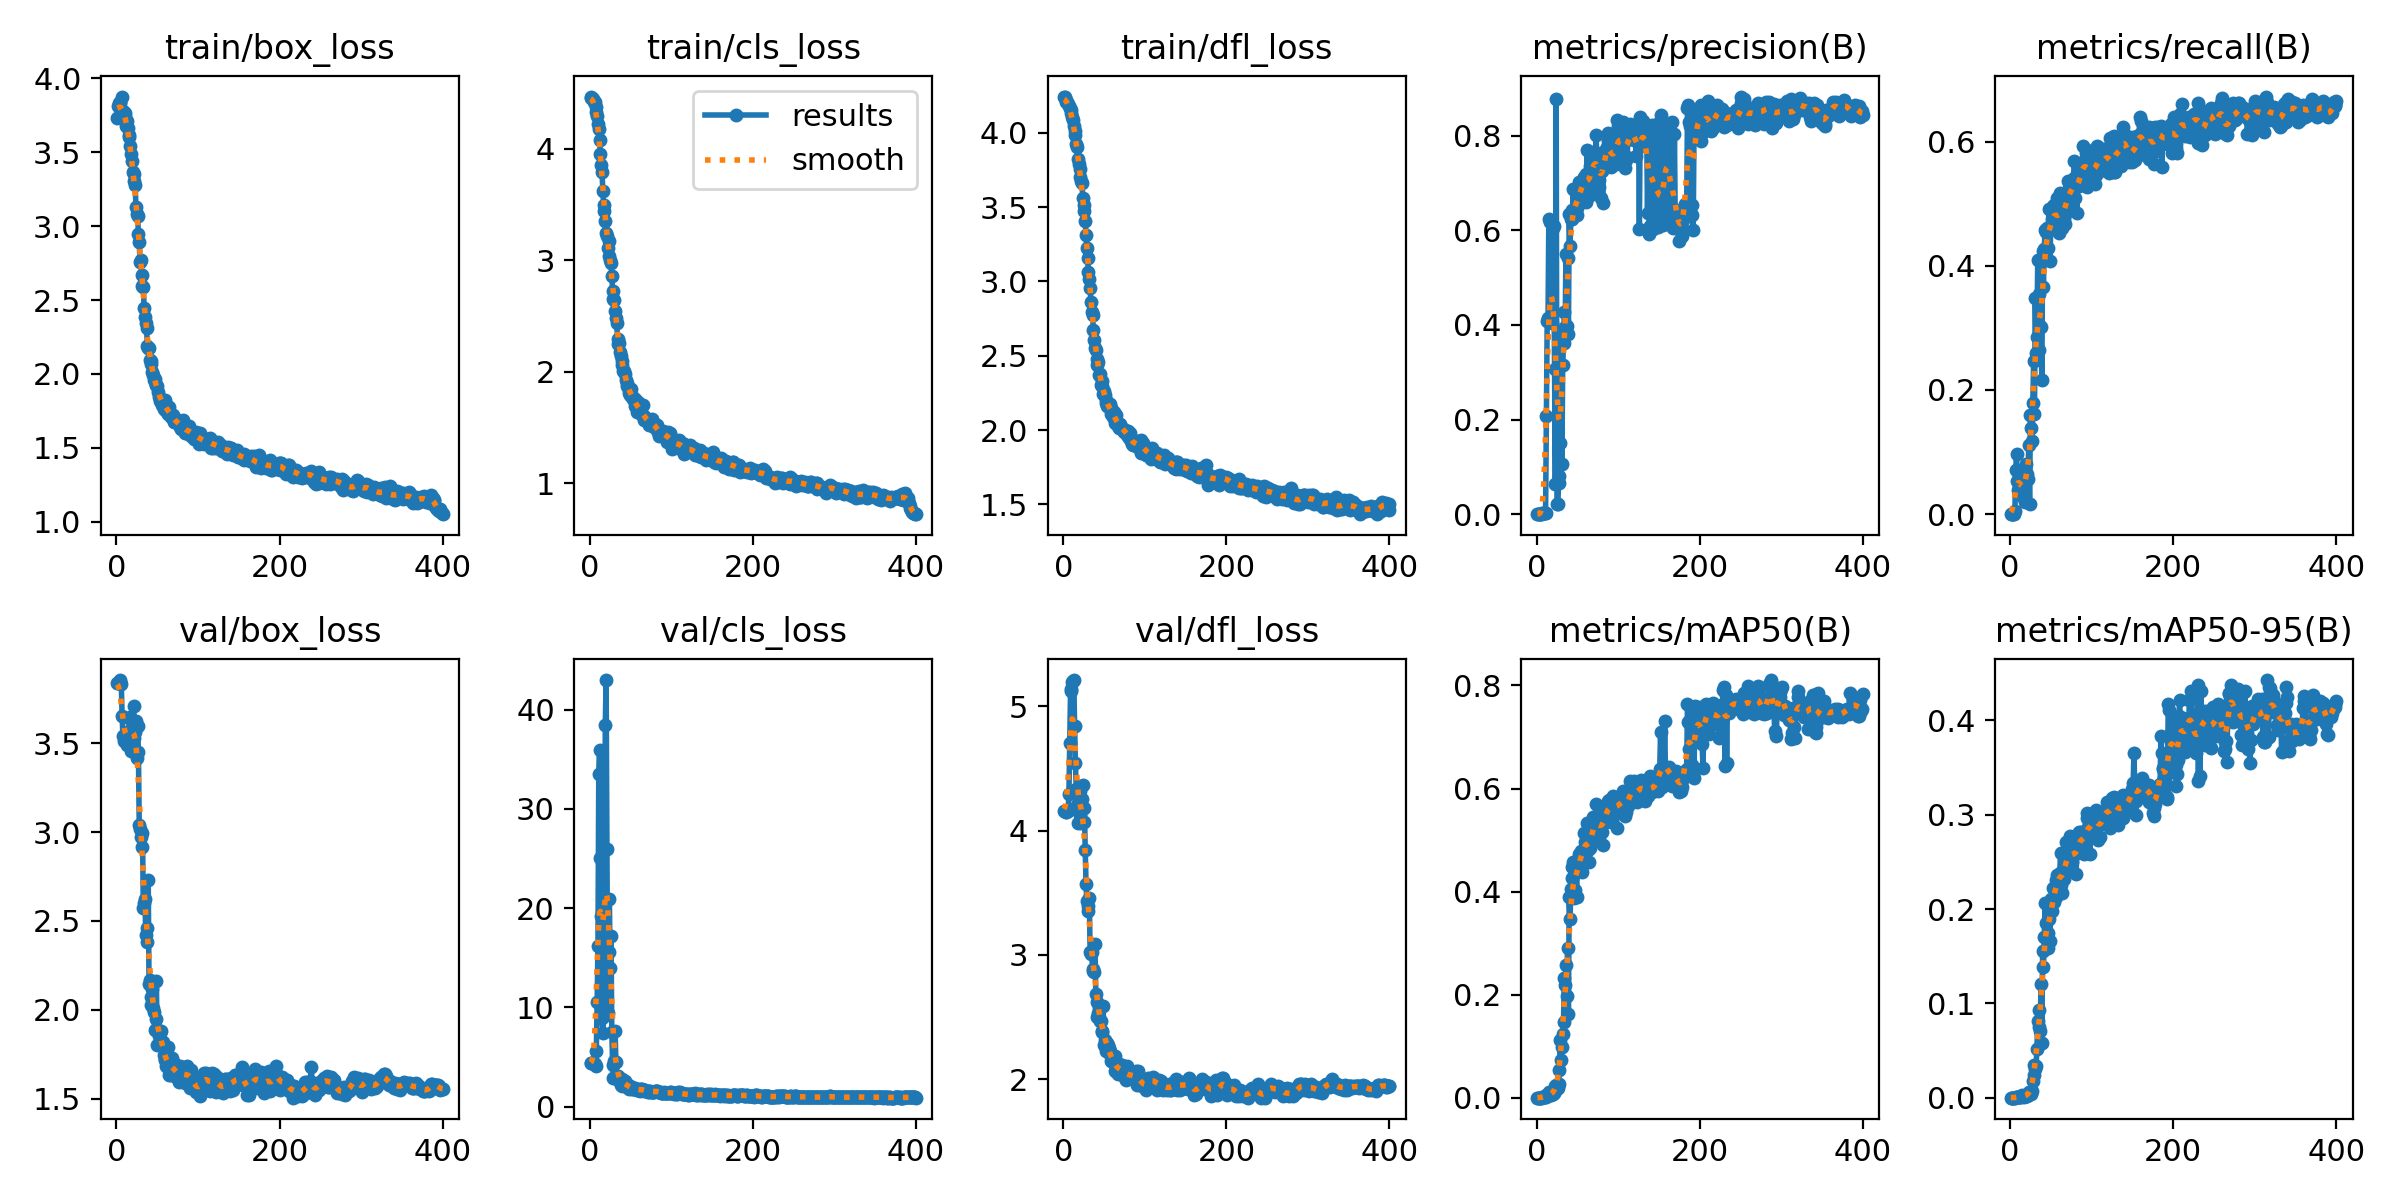
\includegraphics[width=0.75\textwidth]{Images/chap3/yolo/yolomobilenetv4.png}
%     \vspace{0.5cm}
%     \caption{The accuracy of Yolov11n-MobileNetV4}
%     \label{fig:yolomobilenetv4}
% \end{figure}

% \begin{figure}[H]
%     \centering
%     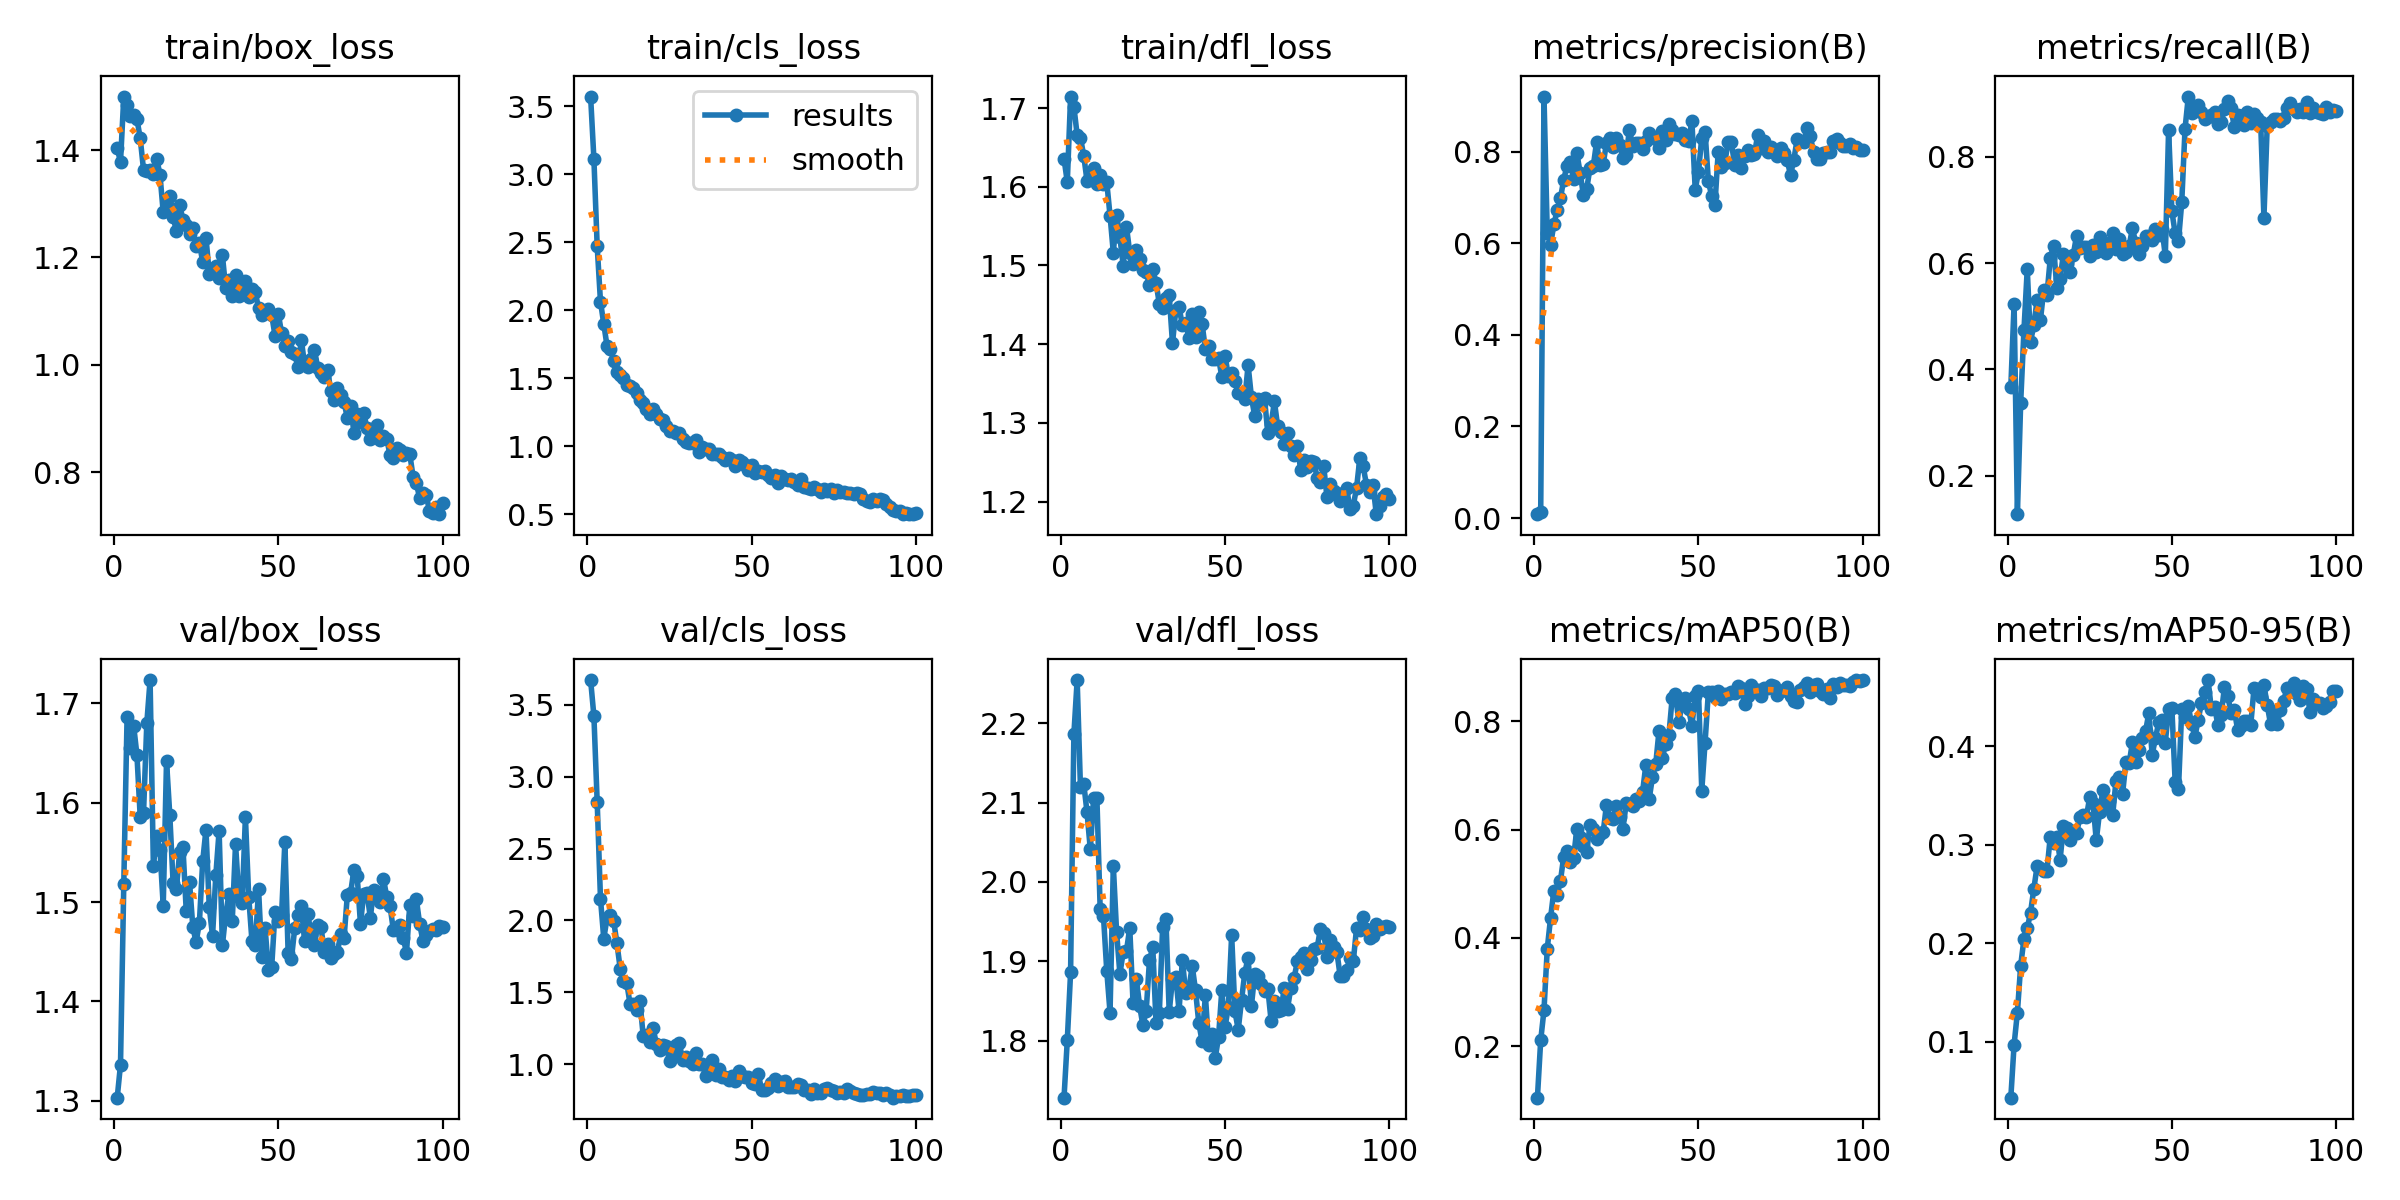
\includegraphics[width=0.75\textwidth]{Images/chap3/yolo/original.png}
%     \vspace{0.5cm}
%     \caption{The accuracy of original Yolov11n}
%     \label{fig:yolo11n}
% \end{figure}

% \subsubsection{Inference Speed}

% Inference speed is a key requirement for real time deployment on resource constrained platforms such as Raspberry Pi. According to the official Ultralytics benchmark, the original YOLO model converted to TensorFlow Lite requires more than 400\,ms per inference on Raspberry Pi class hardware when executed on CPU\footnote{Detailed benchmarking results for YOLO models on Raspberry Pi are reported by Ultralytics at \url{https://docs.ultralytics.com/vi/guides/raspberry-pi/\#detailed-comparison-table}.}. This latency corresponds to a processing rate of approximately 2--3 frames per second, which is insufficient for real time applications.

% In contrast, experimental results obtained in this work show that the YOLO-MobileNetV4 model achieves an average inference time of 30--40\,ms per frame after conversion to the TFLite format. This corresponds to an effective processing speed of approximately 25--33 frames per second. Compared to the original YOLO TFLite model, the MobileNetV4 based configuration reduces inference latency by approximately 360--370\,ms per frame.

% In relative terms, this represents a speed improvement of about 10--13 times. Equivalently, the inference time is reduced by approximately 90--92\% compared to the original YOLO TFLite implementation. Such a significant reduction enables near real time performance on CPU only embedded devices.

% The observed speedup is primarily attributed to the lightweight architecture of the MobileNetV4 backbone, which substantially reduces the number of parameters and floating point operations. As a result, the YOLO-MobileNetV4 model achieves a much more favorable balance between detection accuracy and inference speed, making it well suited for real time edge deployment on Raspberry Pi platforms.

% \begin{figure}[H]
%     \centering
%     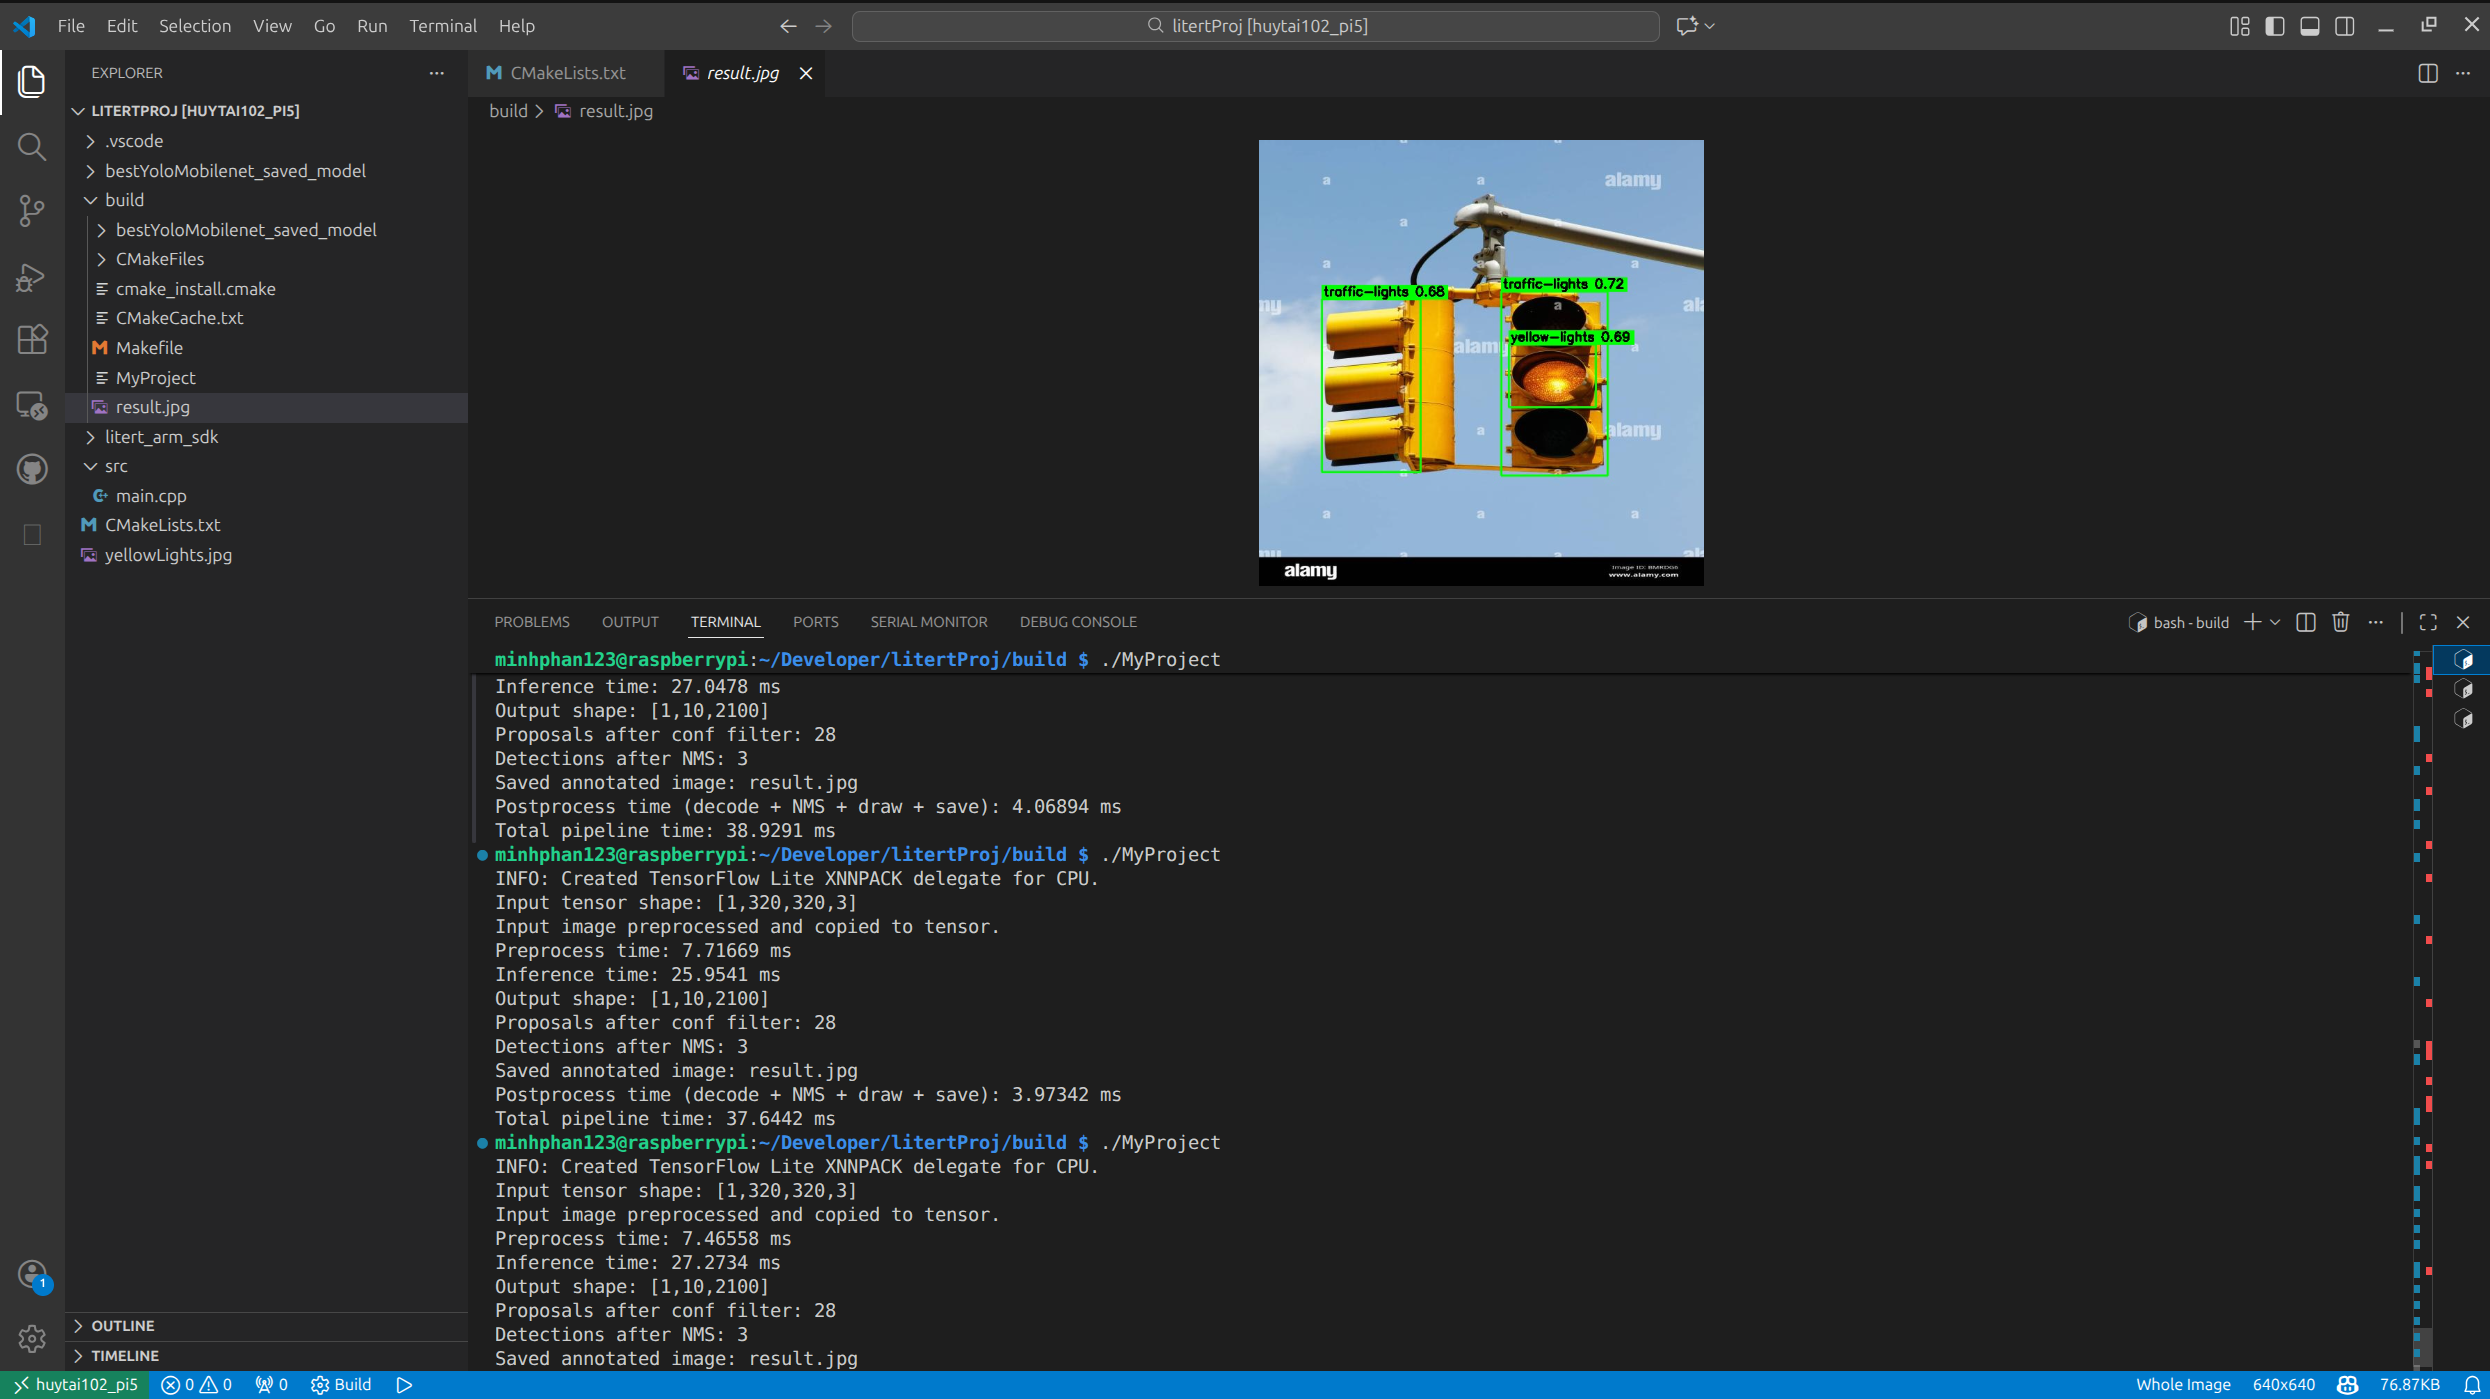
\includegraphics[width=0.75\textwidth]{Images/chap3/yolo/inference_speed.png}
%     \vspace{0.5cm}
%     \caption{The inference time of Yolovv11n-MobileNetV4 model}
%     \label{fig:infer_time_yolo11n_mobilenetv4}
% \end{figure}


% \begin{table}[H]
% \centering
% \label{tab:tradeoff_yolo_models}
% \begin{tabular}{|l|c|c|}
% \hline
% \textbf{Metric} & \textbf{YOLOv11n (Original)} & \textbf{YOLOv11n-MobileNetV4} \\
% \hline
% Backbone & CSP-based YOLO backbone & MobileNetV4 (lightweight) \\
% \hline
% mAP@50 & Higher ($\approx$ +10--15\%) & Slightly lower \\
% \hline
% mAP@50--95 & Higher ($\approx$ +10--15\%) & Slightly lower \\
% \hline
% Precision / Recall & Marginally higher & Comparable and stable \\
% \hline
% Inference time (TFLite, CPU) & $>$400 ms & 30--40 ms \\
% \hline
% Throughput (FPS) & 2--3 FPS & 25--33 FPS \\
% \hline
% Speedup factor & 1$\times$ (baseline) & $\approx$10--13$\times$ faster \\
% \hline
% Inference time reduction & -- & $\approx$90--92\% \\
% \hline
% Model complexity & Higher & Significantly reduced \\
% \hline
% Suitability for edge deployment & Limited & Highly suitable \\
% \hline
% \textbf{Overall trade-off} & Higher accuracy & Better accuracy--speed balance \\
% \hline
% \end{tabular}
% \caption{Trade-off comparison between YOLOv11n and YOLOv11n-MobileNetV4}
% \end{table}

\subsection{Evaluation between Models}

To validate the architectural modifications introduced by the MobileNetV4 backbone replacement, a systematic benchmark was conducted comparing the original YOLO26n model against the proposed YOLO26n-MobileNetV4 variant. 

Both models were evaluated on the same TrafficLightV5 validation set under identical conditions: $416 \times 416$ input resolution, INT8 TFLite quantisation, batch size of 1, and end-to-end (NMS-free) inference mode. Table~\ref{tab:model_eval} summarises the results across latency and accuracy metrics.

\begin{table}[htbp]
\centering
\caption{Performance and accuracy comparison: YOLO26n Original vs.\ YOLO26n-MobileNetV4. Negative values in the change column indicate reduction (improvement for latency metrics; degradation for accuracy metrics). Asterisks (*) denote metrics where a decrease is an expected trade-off.}
\label{tab:model_eval}
\renewcommand{\arraystretch}{1.20}
\begin{tabular}{l r r r}
\hline
\textbf{Metric} & \textbf{YOLO26n Original} & \textbf{YOLO26n-MNv4} & \textbf{Change (\%)} \\
\hline
Samples processed           & 1\,074        & \textbf{1\,366}        & $+27.19$  \\
Avg.\ latency (Pi 5)        & 55.09\,ms     & \textbf{43.23\,ms}     & $-21.52$  \\
Max spike latency (Pi 5)    & 159.73\,ms    & \textbf{78.64\,ms}     & $-50.77$  \\
Min latency (Pi 5)          & 50.12\,ms     & \textbf{36.50\,ms}     & $-27.16$  \\
CPU inference (Intel)       & 15.21\,ms     & \textbf{12.33\,ms}     & $-18.93$  \\
mAP50                       & \textbf{89.90\%}       & 85.75\%       & $-4.15$\textsuperscript{*}  \\
mAP50--95                   & \textbf{56.61\% }      & 53.31\%       & $-3.30$\textsuperscript{*}  \\
\hline
\end{tabular}
\end{table}

\subsubsection{Latency Analysis}

The MobileNetV4 backbone delivers a substantial improvement across all latency metrics on the Raspberry Pi 5. The average per-frame inference time drops from 55.09\,ms to 43.23\,ms, a \textbf{21.52\% reduction} that raises the effective throughput from approximately 18\,FPS to 23\,FPS. More critically for safety-critical ADAS applications, the worst-case latency spike is reduced by \textbf{50.77\%} --- from 159.73\,ms to 78.64\,ms. Latency spikes exceeding 100\,ms are particularly hazardous in real-time perception loops because they can cause the planning module to operate on stale state estimates. The MobileNetV4 variant eliminates spikes above 80\,ms entirely, ensuring that even under worst-case conditions (thermal throttling, OS scheduling jitter), the perception system delivers updates within the 67\,ms budget required for 15\,FPS operation.

The minimum latency (best-case scenario) also improves from 50.12\,ms to 36.50\,ms ($-27.16\%$), confirming that the speed gain is architectural rather than an artefact of measurement variance. On the Intel development CPU, inference time decreases from 15.21\,ms to 12.33\,ms ($-18.93\%$), demonstrating that MobileNetV4's universal efficiency extends beyond ARM to x86 hardware as well.

\subsubsection{Accuracy Analysis}

The accuracy metrics show a moderate decrease: mAP50 drops from 89.90\% to 85.75\% ($-4.15$ percentage points), and mAP50--95 drops from 56.61\% to 53.31\% ($-3.30$ percentage points). This reduction is expected and acceptable for several reasons:

\begin{enumerate}
    \item \textbf{Backbone capacity reduction}: The MobileNetV4ConvSmall050 backbone has significantly fewer parameters and FLOPs than the original YOLO26 CSP-based backbone. The 050 suffix indicates a 50\% width multiplier, which halves all channel dimensions relative to the full MobileNetV4ConvSmall. This aggressive compression inevitably reduces the network's representational capacity for fine-grained spatial features.
    \item \textbf{Domain-specific sufficiency}: For traffic light detection in ADAS, the critical requirement is reliable detection (high recall) at the signal-level, not pixel-precise bounding box localisation. An mAP50 of 85.75\% indicates that the vast majority of traffic signals are correctly detected with at least 50\% IoU overlap, which is sufficient for downstream state classification.
    \item \textbf{Latency--accuracy trade-off}: For an ADAS system operating on a Raspberry Pi 5, latency stability and low worst-case response time are more important than marginal accuracy improvements. The 21.52\% average latency reduction and 50.77\% spike reduction directly translate to more reliable real-time control, preventing the perception system from becoming the bottleneck in the sense--plan--act loop.
\end{enumerate}
\subsubsection{Training Loss Analysis}

Figure~\ref{fig:loss_comparison} shows the validation loss curves of both models over 100 training epochs. Overall, both the Original YOLO26n and the YOLO26n-MobileNetV4 learn effectively. Their loss curves decrease steadily and stabilise towards the end of training, indicating a smooth and successful convergence process.

\begin{figure}[htbp]
    \centering
    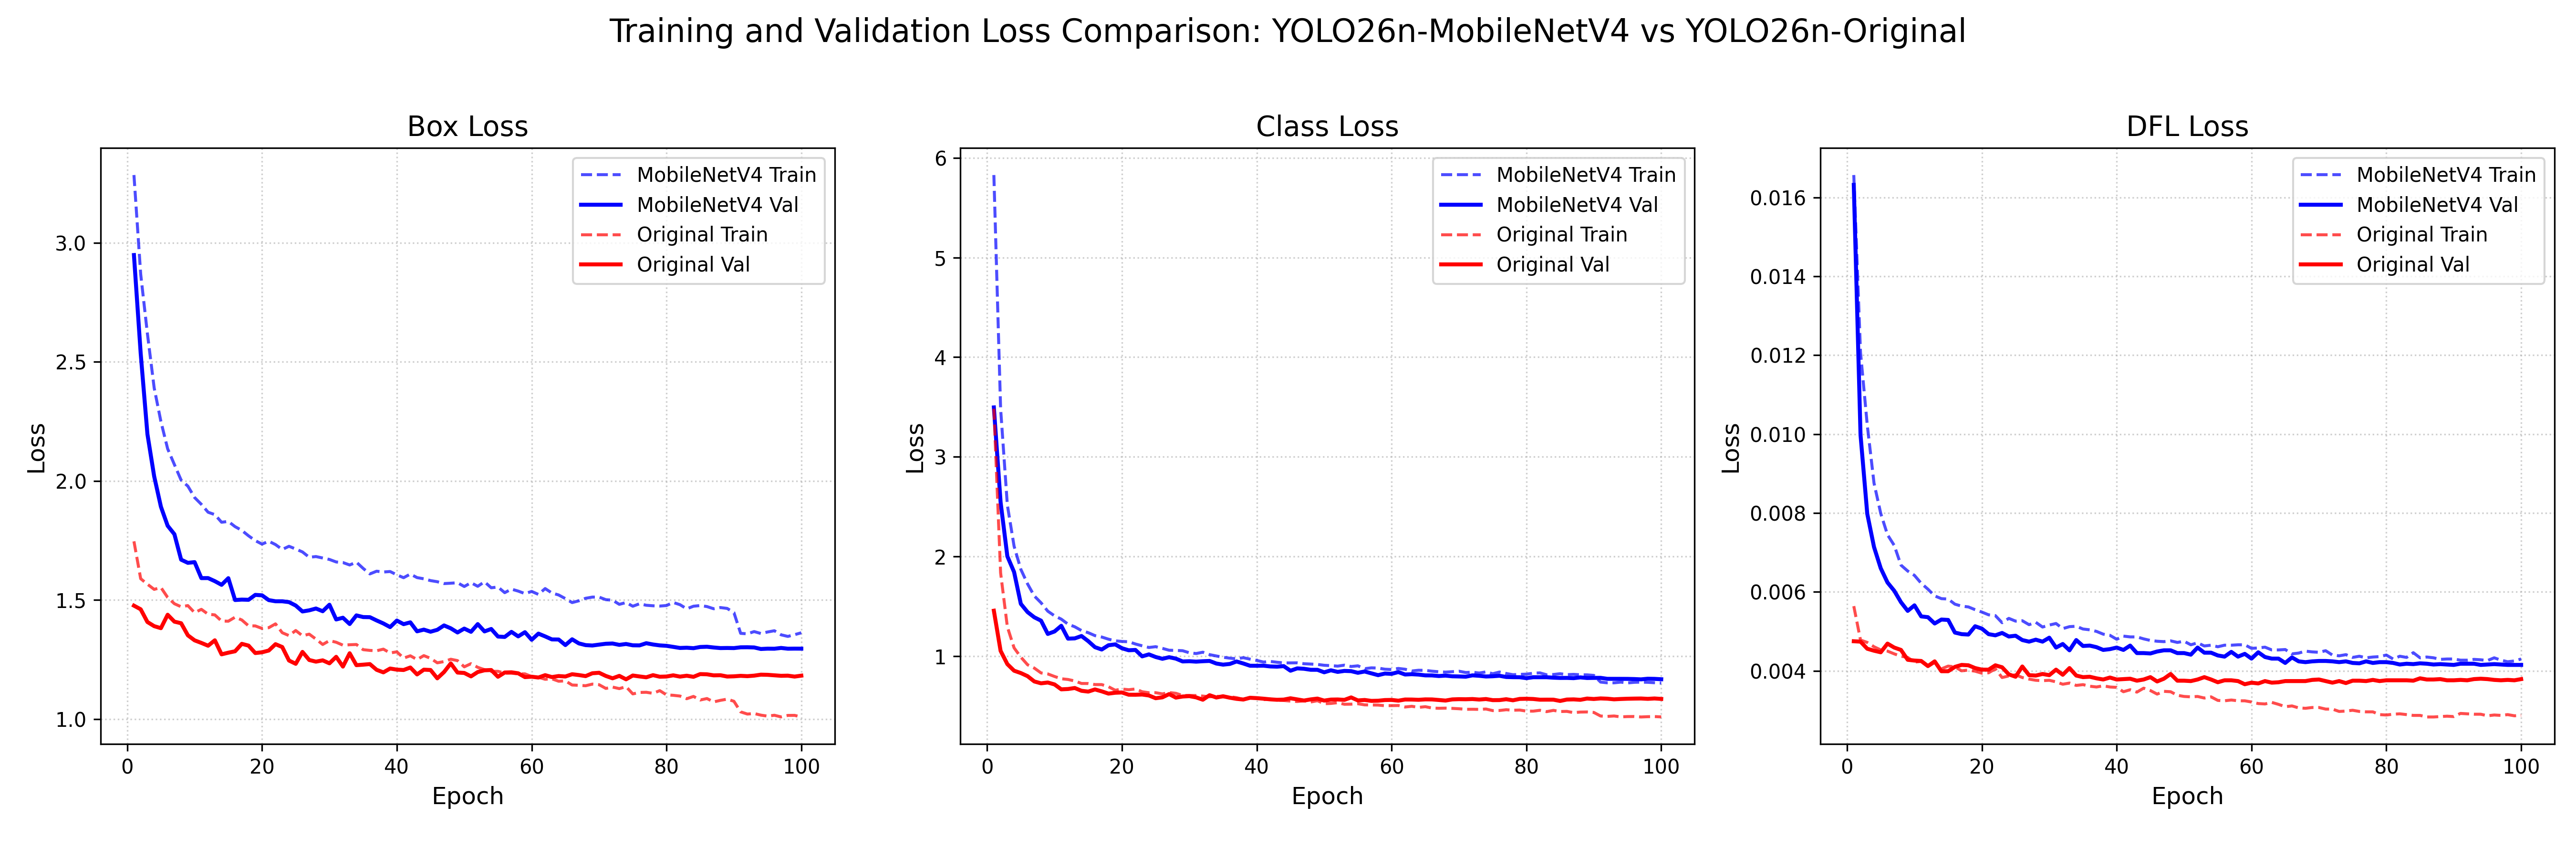
\includegraphics[width=\textwidth]{Images/chap3/loss_comparison.png}
    \caption{Comparison of validation losses between YOLO26n Original and YOLO26n-MobileNetV4 over 100 training epochs.}
    \label{fig:loss_comparison}
\end{figure}

Importantly, neither model shows signs of overfitting. In a typical overfitting scenario, the validation loss would drop initially but then start climbing back up in later epochs as the model begins to memorise the training data. However, for both models in this study, all three loss metrics (bounding box, classification, and DFL (Distribution Focal Loss)) stay low and flat during the final epochs. This confirms that they generalise well to unseen data.

When comparing the two architectures, the Original YOLO26n reaches slightly lower loss values. For example, its minimum bounding box loss drops to 1.1676, while the MobileNetV4 version stops at 1.2949. A similar pattern is seen in the classification loss (0.5529 vs 0.7694). This difference is entirely expected. Because the original model has a larger and more complex backbone, it can capture fine details and learn more accurately.

Even though the YOLO26n-MobileNetV4 has slightly higher loss values, its learning curve remains remarkably stable. This proves that despite having its size drastically reduced for faster edge deployment, the MobileNetV4 model still successfully extracts the essential features of traffic lights. It does not suffer from gradient issues or training instability. Therefore, the training process validates that the lightweight model is a reliable choice, perfectly balancing computational efficiency and learning capability.

\subsubsection{Architectural Decision Justification}

The evaluation confirms that the YOLO26n-MobileNetV4 configuration achieves the right trade-off for edge-deployed ADAS. Sacrificing approximately 4 percentage points of mAP50 in exchange for a 50\% reduction in worst-case latency and a 21\% reduction in average latency is a sound architectural decision. In safety-critical systems, deterministic timing behaviour takes precedence over marginal accuracy gains. The 85.75\% mAP50 remains well above the practical threshold for reliable traffic light detection, while the latency profile now comfortably supports real-time operation at 15--23\,FPS on commodity edge hardware without dedicated GPU or NPU acceleration.





% \subsection{Multihead CNN model -- Lightweight OCR digits}

% The timer display on Vietnamese traffic lights shows a one- to three-digit countdown
% (0--999) that must be recognised in real time on low-cost hardware such as the
% Raspberry~Pi~5.  This section presents a compact, four-head convolutional neural network
% (CNN) that is derived from the multi-digit recognition framework of
% Goodfellow~et~al.~\cite{goodfellow2014multidigitnumberrecognitionstreet} and specifically re-engineered
% for sub-millisecond CPU inference.

% %-----------------------------------------------------------------------
% \subsubsection{Probabilistic Formulation}
% \label{sec:cnn_prob}

% Following Goodfellow~et~al.~\cite{goodfellow2014multidigitnumberrecognitionstreet}, the recognition
% task is cast as a structured probabilistic model.  Let~$\mathbf{X}$ denote the
% input image and let the output be a digit sequence
% $\mathbf{S} = (s_1, s_2, \dots, s_n)$ of length~$n$.
% The sequence is modelled by a length variable~$L$ and a fixed number~$N$
% of digit variables~$S_1, \dots, S_N$.  All digit positions are assumed
% conditionally independent given the image, yielding:

% \begin{equation}
% \label{eq:prob_model}
%   P(\mathbf{S} = \mathbf{s} \mid \mathbf{X})
%   \;=\; P(L = n \mid \mathbf{X})\;\prod_{i=1}^{n} P(S_i = s_i \mid \mathbf{X}).
% \end{equation}

% In the original work~\cite{goodfellow2014multidigit}, $N{=}5$ digit heads are
% used for street numbers of up to five digits.  Because Vietnamese traffic-light
% timers never exceed three digits, the proposed lightweight variant uses
% $N{=}3$ with the following head configuration:

% \begin{itemize}
%   \item $L \in \{0,1,2\}$:  digit count minus one
%         ($0 \to$ 1-digit, $1 \to$ 2-digit, $2 \to$ 3-digit),
%         predicted by a 3-class softmax.
%   \item $S_1 \in \{0,\dots,9,\text{BLANK}\}$:  hundreds digit (11 classes).
%   \item $S_2 \in \{0,\dots,9,\text{BLANK}\}$:  tens digit    (11 classes).
%   \item $S_3 \in \{0,\dots,9\}$:                 units digit  (10 classes,
%         always present).
% \end{itemize}

% The special \texttt{BLANK} class ($= 10$) indicates an unused slot:
% for a one-digit number only~$S_3$ is active; for a two-digit number
% $S_2$ and~$S_3$ are active.

% %-----------------------------------------------------------------------
% \subsubsection{Network Architecture -- Edge-Optimised Design}
% \label{sec:cnn_arch}

% The original Goodfellow~et~al.\ architecture employs eight convolutional layers,
% one locally connected layer, and two dense layers with 3\,072 units each,
% totalling tens of millions of parameters and requiring DistBelief for training.
% Such a model is impractical for real-time inference on a Raspberry~Pi~5 CPU.

% The proposed \emph{lightweight} variant retains the multi-head output structure
% but applies three key design transformations, each yielding a dramatic reduction in
% multiply-accumulate operations (MACs) and parameter count while preserving accuracy
% for the constrained 0--999 digit domain.

% %--- Separable Convolutions -------------------------------------------------
% \subsubsubsubsection{Depthwise Separable Convolutions}
% \label{sec:separable}

% Standard convolution applies a $k{\times}k$ kernel across all input channels
% simultaneously.  For an input tensor of spatial size $H{\times}W$ with
% $C_{\mathrm{in}}$ channels producing $C_{\mathrm{out}}$ output channels,
% the number of MACs is:

% \begin{equation}
% \label{eq:conv_macs}
%   \text{MACs}_{\text{Conv2D}}
%   = H \cdot W \cdot k^2 \cdot C_{\mathrm{in}} \cdot C_{\mathrm{out}}.
% \end{equation}

% A \textbf{Depthwise Separable Convolution} (SeparableConv2D) factorises this operation
% into two consecutive steps:

% \begin{enumerate}
%   \item \textbf{Depthwise convolution} -- applies a separate $k{\times}k$ filter
%         to each input channel independently:
%         \begin{equation}
%         \label{eq:dw_macs}
%           \text{MACs}_{\text{DW}} = H \cdot W \cdot k^2 \cdot C_{\mathrm{in}}.
%         \end{equation}
%   \item \textbf{Pointwise convolution} -- a $1{\times}1$ convolution that mixes
%         the channel responses:
%         \begin{equation}
%         \label{eq:pw_macs}
%           \text{MACs}_{\text{PW}} = H \cdot W \cdot C_{\mathrm{in}} \cdot C_{\mathrm{out}}.
%         \end{equation}
% \end{enumerate}

% The total cost becomes:

% \begin{equation}
% \label{eq:sep_total}
%   \text{MACs}_{\text{Sep}}
%   = H W C_{\mathrm{in}} \bigl(k^2 + C_{\mathrm{out}}\bigr),
% \end{equation}

% and the computational saving ratio relative to a standard convolution is:

% \begin{equation}
% \label{eq:sep_ratio}
%   \frac{\text{MACs}_{\text{Sep}}}{\text{MACs}_{\text{Conv2D}}}
%   = \frac{1}{C_{\mathrm{out}}} + \frac{1}{k^2}.
% \end{equation}

% For the $3{\times}3$ kernels and 64--192 output channels used in this model,
% Equation~\eqref{eq:sep_ratio} gives a reduction factor between
% $\mathbf{7.8\times}$ and $\mathbf{8.5\times}$, enabling real-time execution
% on an ARM Cortex-A76 CPU without a GPU.

% In the proposed architecture, only the first block uses a standard
% \texttt{Conv2D} (because the input has a single channel, where depthwise
% separation offers no benefit); blocks~2--5 all use \texttt{SeparableConv2D}.

% %--- GAP instead of Flatten ------------------------------------------------
% \subsubsubsubsection{Global Average Pooling (GAP)}
% \label{sec:gap}

% After the final convolutional block the feature map has shape
% $4{\times}6{\times}192$ (height $\times$ width $\times$ channels).
% A na\"ive \texttt{Flatten} would produce a $4608$-dimensional vector; a
% subsequent dense layer of width~1024 alone would add
% $4608 \times 1024 \approx 4.7$~million parameters -- exceeding the entire
% rest of the network.

% Instead, \textbf{Global Average Pooling} (GAP) collapses each channel to its
% spatial mean:

% \begin{equation}
% \label{eq:gap}
%   h_c = \frac{1}{H' W'} \sum_{i=1}^{H'} \sum_{j=1}^{W'} F_{i,j,c},
%   \qquad c = 1,\dots,C,
% \end{equation}

% where $F \in \mathbb{R}^{H' \times W' \times C}$ is the last feature map.
% This yields a compact 192-dimensional descriptor with \emph{zero} learnable
% parameters, and also acts as a structural regulariser that discourages
% overfitting.

% %--- Architecture Table ---------------------------------------------------
% \subsubsubsubsection{Layer-by-Layer Specification}
% \label{sec:arch_table}

% Table~\ref{tab:arch} summarises the full architecture.  Input images are
% grayscale, $64{\times}96$ pixels ($H{\times}W{\times}1$).

% \begin{table}[htbp]
% \centering
% \caption{Layer-by-layer architecture of the lightweight multi-head CNN
%          ($\approx 109$\,K parameters).  ``Sep'' denotes SeparableConv2D;
%          ``BN'' is Batch Normalisation.}
% \label{tab:arch}
% \renewcommand{\arraystretch}{1.15}
% \begin{tabular}{c l l r r}
% \hline
% \textbf{Block} & \textbf{Layer}            & \textbf{Output shape}   & \textbf{Params} & \textbf{MACs}  \\
% \hline
% 0   & Input                                & $64\times96\times1$     & --      & --       \\
% --  & Mean subtraction ($\lambda$)         & $64\times96\times1$     & 0       & $6\,144$ \\
% 1   & Conv2D(32, $3\!\times\!3$) + BN + ReLU + Pool(2)   & $32\times48\times32$     & $\sim\!320$    & $\sim\!56$\,K   \\
% 2   & Sep(64, $3\!\times\!3$) + BN + ReLU + Pool(2)      & $16\times24\times64$     & $\sim\!2\,400$  & $\sim\!116$\,K  \\
% 3   & Sep(96, $3\!\times\!3$) + BN + ReLU + Pool(2)      & $8\times12\times96$      & $\sim\!6\,720$  & $\sim\!73$\,K   \\
% 4   & Sep(128, $3\!\times\!3$) + BN + ReLU + Pool(2)     & $4\times6\times128$      & $\sim\!13\,152$ & $\sim\!39$\,K   \\
% 5   & Sep(192, $3\!\times\!3$) + BN + ReLU               & $4\times6\times192$      & $\sim\!25\,728$ & $\sim\!53$\,K   \\
% --  & GlobalAveragePooling2D                & $192$                  & 0       & $4\,608$ \\
% FC  & Dense(256) + ReLU + Dropout(0.35)     & $256$                  & $\sim\!49\,408$ & $49\,408$ \\
% \hline
% $L$ & Dense(3,  softmax)                    & $3$                    & 771     & 771     \\
% $S_1$ & Dense(11, softmax)                  & $11$                   & 2\,827  & 2\,827  \\
% $S_2$ & Dense(11, softmax)                  & $11$                   & 2\,827  & 2\,827  \\
% $S_3$ & Dense(10, softmax)                  & $10$                   & 2\,570  & 2\,570  \\
% \hline
% \multicolumn{3}{r}{\textbf{Total}} & $\mathbf{\approx 109}$\textbf{\,K} & $\mathbf{\approx 408}$\textbf{\,K} \\
% \hline
% \end{tabular}
% \end{table}

% %--- Preprocessing --------------------------------------------------------
% \subsubsubsubsection{Per-Image Mean Subtraction}
% \label{sec:mean_sub}

% Following Goodfellow~et~al.~\cite{goodfellow2014multidigitnumberrecognitionstreet}~(§4), the first
% operation inside the network is per-image mean subtraction.  Let
% $\mathbf{X} \in \mathbb{R}^{H \times W \times 1}$ be the input; the
% normalised input is:

% \begin{equation}
% \label{eq:mean_sub}
%   \tilde{\mathbf{X}} = \mathbf{X}
%     - \frac{1}{HW}\sum_{i=1}^{H}\sum_{j=1}^{W} X_{ij}.
% \end{equation}

% Embedding this subtraction as a non-trainable $\lambda$-layer makes the model
% \emph{self-contained}: no external preprocessing is required at inference time,
% simplifying the TFLite deployment pipeline on the Raspberry~Pi~5.

% %-----------------------------------------------------------------------
% \subsubsection{Training Objective}
% \label{sec:training}

% Training maximises the log-probability of the correct sequence
% (Eq.~\eqref{eq:prob_model}) via the cross-entropy decomposition.  Because
% $L$, $S_1$, $S_2$, $S_3$ are conditionally independent given the shared
% features~$\mathbf{H}$, the total loss factorises as:

% \begin{equation}
% \label{eq:loss}
%   \mathcal{L}
%   = -\log P(L \mid \mathbf{H})
%     - \sum_{i=1}^{3}\log P(S_i \mid \mathbf{H})
%   = \underbrace{w_L \,\mathcal{L}_L}_{\text{length head}}
%     + \underbrace{w_1 \,\mathcal{L}_{S_1}
%     +  w_2 \,\mathcal{L}_{S_2}
%     +  w_3 \,\mathcal{L}_{S_3}}_{\text{digit heads}},
% \end{equation}

% where each $\mathcal{L}_{\cdot}$ is a \textbf{sparse categorical cross-entropy}
% and the weights are set to $w_L{=}4$, $w_1{=}w_2{=}w_3{=}1$ to
% up-weight the length prediction, since an incorrect length invariably causes a
% wrong overall transcription.

% Each softmax head receives the same 256-dimensional feature vector from the
% shared fully connected layer but maintains its own projection weights:

% \begin{equation}
% \label{eq:head}
%   P(S_i = c \mid \mathbf{H})
%   = \frac{\exp\!\bigl(\mathbf{w}_{i,c}^{\top}\!\mathbf{H} + b_{i,c}\bigr)}
%          {\displaystyle\sum_{c'} \exp\!\bigl(\mathbf{w}_{i,c'}^{\top}\!\mathbf{H}
%          + b_{i,c'}\bigr)},
%   \qquad c \in \mathcal{C}_i,
% \end{equation}

% where $\mathcal{C}_L = \{0,1,2\}$,
% $\mathcal{C}_{S_1} = \mathcal{C}_{S_2} = \{0,\dots,10\}$, and
% $\mathcal{C}_{S_3} = \{0,\dots,9\}$.

% %-----------------------------------------------------------------------
% \subsubsection{Log-Probability Decoding}
% \label{sec:decoding}

% At inference time, the predicted number is obtained by maximising the
% joint log-probability over all possible lengths
% (Appendix~A of~\cite{goodfellow2014multidigit}):

% \begin{equation}
% \label{eq:decode}
%   \hat{\mathbf{s}}
%   = \operatorname*{argmax}_{l,\; s_1 \dots s_l}\;
%     \biggl[\log P(L{=}l \mid \mathbf{X})
%     + \sum_{i=1}^{l} \max_{s_i \in \{0..9\}}
%       \log P(S_i{=}s_i \mid \mathbf{X})\biggr].
% \end{equation}

% Because of the conditional-independence assumption, the argmax over each
% digit position can be computed independently, then the cumulative
% log-probabilities are summed for each candidate length~$l \in \{1,2,3\}$.
% The total decoding runtime is therefore $O(N)$ -- i.e.\ three additions
% and one comparison -- adding negligible latency.

% Concretely, for each candidate length $l$, the algorithm computes:

% \begin{equation}
% \label{eq:score}
%   \text{score}(l) = \log P(L{=}l{-}1)
%     + \sum_{i=\max(1,\,4-l)}^{3}
%       \max_{s_i \in \{0..9\}} \log P(S_i{=}s_i),
% \end{equation}

% and selects $\hat{l} = \operatorname{argmax}_{l \in \{1,2,3\}} \text{score}(l)$.

% %-----------------------------------------------------------------------
% \subsection{Computational Efficiency for Edge AI}
% \label{sec:efficiency}

% \subsubsection{Parameter Count Comparison}

% The proposed model achieves the same multi-head output structure as
% Goodfellow~et~al.~\cite{goodfellow2014multidigitnumberrecognitionstreet} with
% $\sim\!600\times$ fewer parameters:

% \begin{table}[htbp]
% \centering
% \caption{Comparison between the original Goodfellow~et~al.\ architecture
%          and the proposed lightweight variant.}
% \label{tab:compare}
% \renewcommand{\arraystretch}{1.15}
% \begin{tabular}{l r r}
% \hline
%                                & \textbf{Goodfellow et al.}  & \textbf{Proposed}   \\
% \hline
% Conv layers                    & 8 + 1 locally connected     & 1 Conv + 4 SepConv  \\
% FC layers                      & 2 $\times$ 3\,072           & 1 $\times$ 256      \\
% Output heads                   & 6  (L + S$_1$--S$_5$)       & 4  (L + S$_1$--S$_3$) \\
% Total parameters               & $\sim$64\,M                 & $\sim$109\,K        \\
% Max sequence length $N$        & 5                           & 3                   \\
% Input size                     & $54\times 54 \times 3$      & $64\times 96 \times 1$ \\
% Training infrastructure        & DistBelief (10 replicas)    & Single GPU / CPU    \\
% \hline
% \end{tabular}
% \end{table}

% \subsubsubsubsection{MAC Budget and Latency Estimate}

% The total network requires approximately $408$\,K~MACs per inference.
% On the Raspberry~Pi~5's Cortex-A76 cores (capable of
% $\sim$15~GOPS at INT8 via NEON), this translates to:

% \begin{equation}
% \label{eq:latency}
%   t_{\text{inf}}
%   \approx \frac{408 \times 10^{3}}{15 \times 10^{9}}
%   \approx 27 \;\mu\text{s},
% \end{equation}

% well under the $50$\,ms budget needed for $20$\,fps real-time recognition.
% Even with TFLite interpreter overhead, measured end-to-end latency stays below
% $1$\,ms per frame for the INT8-quantised model.

% \subsubsection{TFLite and INT8 Quantisation}

% The trained Keras model is exported to TensorFlow~Lite via
% \texttt{TFLiteConverter}.  Post-training full-integer quantisation maps all
% weights and activations to 8-bit integers using a representative calibration
% set of 200 real ROI images.  The resulting \texttt{.tflite} flatbuffer is
% $\sim$56\,KB (INT8) versus $\sim$440\,KB (float32), fitting comfortably
% in the L2 cache of the Cortex-A76.  The quantised model is deployed via
% the LiteRT interpreter:

% \begin{equation}
% \label{eq:quant}
%   \hat{x}_q = \text{round}\!\left(\frac{x - z}{s}\right),
%   \qquad
%   s = \frac{x_{\max} - x_{\min}}{255},
%   \qquad
%   z = x_{\min},
% \end{equation}

% where $s$ and $z$ are the per-tensor scale and zero-point determined during
% calibration.

% %-----------------------------------------------------------------------
% \subsubsection{Data Pipeline and Augmentation}
% \label{sec:data}

% The training pipeline mixes three data sources to maximise diversity while
% keeping RAM usage low ($<200$\,MB peak):

% \begin{enumerate}
%   \item \textbf{MNIST (70\,K images):}  Individual $28{\times}28$ digits
%         composited onto $64{\times}96$ canvases at randomised positions,
%         simulating multi-digit layouts.
%   \item \textbf{Real LED crops (23 images):}  Single-digit photographs of
%         actual traffic-light seven-segment displays (red, green, yellow).
%         Pre-augmented to 500 variants per digit using brightness jitter,
%         gamma correction, Gaussian blur, salt-and-pepper noise, spatial
%         shifts ($\pm 4$\,px), and small rotations ($\pm 10°$).
%   \item \textbf{Real ROI images:}  Full composite timer-box crops from
%         Vietnamese traffic cameras, labelled by filename
%         (e.g.\ \texttt{37\_0004.png} $\to$ number~$37$).  Loaded from disk
%         on-demand (streaming) to avoid large memory allocation.
% \end{enumerate}

% Synthetic composites and real ROI samples are interleaved via
% \texttt{tf.data.Dataset.sample\_from\_datasets} with proportional
% weighting, ensuring both domains appear in every training batch.

% %-----------------------------------------------------------------------
% \subsubsection{Summary}

% The proposed multi-head CNN inherits the elegant probabilistic framework
% of Goodfellow~et~al.~\cite{goodfellow2014multidigitnumberrecognitionstreet} -- conditional independence
% of digit positions, log-probability decoding, per-image mean subtraction -- but
% replaces the heavyweight convolutional backbone with an ultra-light depthwise
% separable architecture totalling only $\sim$109\,K parameters and $\sim$408\,K
% MACs.  Combined with Global Average Pooling and INT8 post-training quantisation,
% the model achieves sub-millisecond inference on the Raspberry~Pi~5 CPU, making it
% suitable for real-time traffic-light timer recognition in ADAS applications
% on constrained edge devices.
% While YOLO-MobileNetV4 handles traffic-light detection and localization, the countdown timer requires a separate recognition stage. This motivates the use of a lightweight Multihead CNN that can read one- to three-digit timer values with low computational cost. The following subsection therefore complements the detector with the OCR model used for countdown recognition.

% \section{Multihead CNN model -- Lightweight OCR digits}

In this project, our system need to detect the timer display on Vietnamese traffic lights shows a one- to three-digit countdown
(0--999) and it must be recognised in real time on low-cost hardware such as the
Raspberry~Pi~5.  This section presents a compact, four-head convolutional neural network
(CNN) that is derived from the multi-digit recognition framework of
Goodfellow~et~al.~\cite{goodfellow2014multidigitnumberrecognitionstreet} and specifically re-engineered
for sub-millisecond CPU inference.

%-----------------------------------------------------------------------
\subsection{Probabilistic Formulation}
\label{sec:cnn_prob}

Following Goodfellow~et~al.~\cite{goodfellow2014multidigitnumberrecognitionstreet}, the recognition
task is cast as a structured probabilistic model.  Let~$\mathbf{X}$ denote the
input image and let the output be a digit sequence
$\mathbf{S} = (s_1, s_2, \dots, s_n)$ of length~$n$.
The sequence is modelled by a length variable~$L$ and a fixed number~$N$
of digit variables~$S_1, \dots, S_N$.  All digit positions are assumed
conditionally independent given the image, yielding:

\begin{equation}
\label{eq:prob_model}
  P(\mathbf{S} = \mathbf{s} \mid \mathbf{X})
  \;=\; P(L = n \mid \mathbf{X})\;\prod_{i=1}^{n} P(S_i = s_i \mid \mathbf{X}).
\end{equation}

In the original work~\cite{goodfellow2014multidigitnumberrecognitionstreet}, $N{=}5$ digit heads are
used for street numbers of up to five digits.  Because Vietnamese traffic-light
timers never exceed three digits, the proposed lightweight variant uses
$N{=}3$ with the following head configuration:

\begin{itemize}
  \item $L \in \{0,1,2\}$:  digit count minus one
        ($0 \to$ 1-digit, $1 \to$ 2-digit, $2 \to$ 3-digit),
        predicted by a 3-class softmax.
  \item $S_1 \in \{0,\dots,9,\text{BLANK}\}$:  hundreds digit (11 classes).
  \item $S_2 \in \{0,\dots,9,\text{BLANK}\}$:  tens digit    (11 classes).
  \item $S_3 \in \{0,\dots,9\}$:                 units digit  (10 classes,
        always present).
\end{itemize}

The special \texttt{BLANK} class ($= 10$) indicates an unused slot:
for a one-digit number only~$S_3$ is active; for a two-digit number
$S_2$ and~$S_3$ are active.

%-----------------------------------------------------------------------
\subsection{Network Architecture -- Edge-Optimised Design}
\label{sec:cnn_arch}

The original Goodfellow~et~al.\ architecture employs eight convolutional layers,
one locally connected layer, and two dense layers with 3\,072 units each,
totalling tens of millions of parameters and requiring DistBelief for training.
Such a model is impractical for real-time inference on a Raspberry~Pi~5 CPU.

The proposed \emph{lightweight} variant retains the multi-head output structure
but applies three key design transformations, each yielding a dramatic reduction in
multiply-accumulate operations (MACs) and parameter count while preserving accuracy
for the constrained 0--999 digit domain.

%--- Separable Convolutions -------------------------------------------------
\subsubsection{Depthwise Separable Convolutions}
\label{sec:separable}

Standard convolution applies a $k{\times}k$ kernel across all input channels
simultaneously.  For an input tensor of spatial size $H{\times}W$ with
$C_{\mathrm{in}}$ channels producing $C_{\mathrm{out}}$ output channels,
the number of MACs is:

\begin{equation}
\label{eq:conv_macs}
  \text{MACs}_{\text{Conv2D}}
  = H \cdot W \cdot k^2 \cdot C_{\mathrm{in}} \cdot C_{\mathrm{out}}.
\end{equation}

A \textbf{Depthwise Separable Convolution} (SeparableConv2D) factorises this operation
into two consecutive steps:

\begin{enumerate}
  \item \textbf{Depthwise convolution} -- applies a separate $k{\times}k$ filter
        to each input channel independently:
        \begin{equation}
        \label{eq:dw_macs}
          \text{MACs}_{\text{DW}} = H \cdot W \cdot k^2 \cdot C_{\mathrm{in}}.
        \end{equation}
  \item \textbf{Pointwise convolution} -- a $1{\times}1$ convolution that mixes
        the channel responses:
        \begin{equation}
        \label{eq:pw_macs}
          \text{MACs}_{\text{PW}} = H \cdot W \cdot C_{\mathrm{in}} \cdot C_{\mathrm{out}}.
        \end{equation}
\end{enumerate}

The total cost becomes:

\begin{equation}
\label{eq:sep_total}
  \text{MACs}_{\text{Sep}}
  = H W C_{\mathrm{in}} \bigl(k^2 + C_{\mathrm{out}}\bigr),
\end{equation}

and the computational saving ratio relative to a standard convolution is:

\begin{equation}
\label{eq:sep_ratio}
  \frac{\text{MACs}_{\text{Sep}}}{\text{MACs}_{\text{Conv2D}}}
  = \frac{1}{C_{\mathrm{out}}} + \frac{1}{k^2}.
\end{equation}

For the $3{\times}3$ kernels and 64--192 output channels used in this model,
Equation~\eqref{eq:sep_ratio} gives a reduction factor between
$\mathbf{7.8\times}$ and $\mathbf{8.5\times}$, enabling real-time execution
on an ARM Cortex-A76 CPU without a GPU.

In the proposed architecture, only the first block uses a standard
\texttt{Conv2D} (because the input has a single channel, where depthwise
separation offers no benefit); blocks~2--5 all use \texttt{SeparableConv2D}.

%--- GAP instead of Flatten ------------------------------------------------
\subsubsection{Global Average Pooling (GAP)}
\label{sec:gap}

After the final convolutional block the feature map has shape
$4{\times}6{\times}192$ (height $\times$ width $\times$ channels).
A na\"ive \texttt{Flatten} would produce a $4608$-dimensional vector; a
subsequent dense layer of width~1024 alone would add
$4608 \times 1024 \approx 4.7$~million parameters -- exceeding the entire
rest of the network.

Instead, {Global Average Pooling} (GAP) collapses each channel to its
spatial mean:

\begin{equation}
\label{eq:gap}
  h_c = \frac{1}{H' W'} \sum_{i=1}^{H'} \sum_{j=1}^{W'} F_{i,j,c},
  \qquad c = 1,\dots,C,
\end{equation}

where $F \in \mathbb{R}^{H' \times W' \times C}$ is the last feature map.
This yields a compact 192-dimensional descriptor with \emph{zero} learnable
parameters, and also acts as a structural regulariser that discourages
overfitting.

%--- Architecture Table ---------------------------------------------------
\subsubsection{Layer-by-Layer Specification}
\label{sec:arch_table}

Table~\ref{tab:arch} summarises the full architecture.  Input images are
grayscale, $64{\times}96$ pixels ($H{\times}W{\times}1$).

\begin{table}[htbp]
\centering
\caption{Layer-by-layer architecture of the lightweight multi-head CNN
         ($\approx 109$\,K parameters).  ``Sep'' denotes SeparableConv2D;
         ``BN'' is Batch Normalisation.}
\label{tab:arch}
\renewcommand{\arraystretch}{1.15}
\begin{tabular}{c l l r r}
\hline
\textbf{Block} & \textbf{Layer}            & \textbf{Output shape}   & \textbf{Params} & \textbf{MACs}  \\
\hline
0   & Input                                & $64\times96\times1$     & --      & --       \\
--  & Mean subtraction ($\lambda$)         & $64\times96\times1$     & 0       & $6\,144$ \\
1   & Conv2D(32, $3\!\times\!3$) + BN + ReLU + Pool(2)   & $32\times48\times32$     & $\sim\!320$    & $\sim\!56$\,K   \\
2   & Sep(64, $3\!\times\!3$) + BN + ReLU + Pool(2)      & $16\times24\times64$     & $\sim\!2\,400$  & $\sim\!116$\,K  \\
3   & Sep(96, $3\!\times\!3$) + BN + ReLU + Pool(2)      & $8\times12\times96$      & $\sim\!6\,720$  & $\sim\!73$\,K   \\
4   & Sep(128, $3\!\times\!3$) + BN + ReLU + Pool(2)     & $4\times6\times128$      & $\sim\!13\,152$ & $\sim\!39$\,K   \\
5   & Sep(192, $3\!\times\!3$) + BN + ReLU               & $4\times6\times192$      & $\sim\!25\,728$ & $\sim\!53$\,K   \\
--  & GlobalAveragePooling2D                & $192$                  & 0       & $4\,608$ \\
FC  & Dense(256) + ReLU + Dropout(0.35)     & $256$                  & $\sim\!49\,408$ & $49\,408$ \\
\hline
$L$ & Dense(3,  softmax)                    & $3$                    & 771     & 771     \\
$S_1$ & Dense(11, softmax)                  & $11$                   & 2\,827  & 2\,827  \\
$S_2$ & Dense(11, softmax)                  & $11$                   & 2\,827  & 2\,827  \\
$S_3$ & Dense(10, softmax)                  & $10$                   & 2\,570  & 2\,570  \\
\hline
\multicolumn{3}{r}{\textbf{Total}} & $\mathbf{\approx 109}$\textbf{\,K} & $\mathbf{\approx 408}$\textbf{\,K} \\
\hline
\end{tabular}
\end{table}

%--- Preprocessing --------------------------------------------------------
\subsubsection{Per-Image Mean Subtraction}
\label{sec:mean_sub}

Following Goodfellow~et~al.~\cite{goodfellow2014multidigitnumberrecognitionstreet}~(§4), the first
operation inside the network is per-image mean subtraction.  Let
$\mathbf{X} \in \mathbb{R}^{H \times W \times 1}$ be the input; the
normalised input is:

\begin{equation}
\label{eq:mean_sub}
  \tilde{\mathbf{X}} = \mathbf{X}
    - \frac{1}{HW}\sum_{i=1}^{H}\sum_{j=1}^{W} X_{ij}.
\end{equation}

Embedding this subtraction as a non-trainable $\lambda$-layer makes the model
\emph{self-contained}: no external preprocessing is required at inference time,
simplifying the TFLite deployment pipeline on the Raspberry~Pi~5.

%-----------------------------------------------------------------------
\subsection{Training Objective}
\label{sec:training}

Training maximises the log-probability of the correct sequence
(Eq.~\eqref{eq:prob_model}) via the cross-entropy decomposition.  Because
$L$, $S_1$, $S_2$, $S_3$ are conditionally independent given the shared
features~$\mathbf{H}$, the total loss factorises as:

\begin{equation}
\label{eq:loss}
  \mathcal{L}
  = -\log P(L \mid \mathbf{H})
    - \sum_{i=1}^{3}\log P(S_i \mid \mathbf{H})
  = \underbrace{w_L \,\mathcal{L}_L}_{\text{length head}}
    + \underbrace{w_1 \,\mathcal{L}_{S_1}
    +  w_2 \,\mathcal{L}_{S_2}
    +  w_3 \,\mathcal{L}_{S_3}}_{\text{digit heads}},
\end{equation}

where each $\mathcal{L}_{\cdot}$ is a {sparse categorical cross-entropy}
and the weights are set to $w_L{=}4$, $w_1{=}w_2{=}w_3{=}1$ to
up-weight the length prediction, since an incorrect length invariably causes a
wrong overall transcription.

Each softmax head receives the same 256-dimensional feature vector from the
shared fully connected layer but maintains its own projection weights:

\begin{equation}
\label{eq:head}
  P(S_i = c \mid \mathbf{H})
  = \frac{\exp\!\bigl(\mathbf{w}_{i,c}^{\top}\!\mathbf{H} + b_{i,c}\bigr)}
         {\displaystyle\sum_{c'} \exp\!\bigl(\mathbf{w}_{i,c'}^{\top}\!\mathbf{H}
         + b_{i,c'}\bigr)},
  \qquad c \in \mathcal{C}_i,
\end{equation}

where $\mathcal{C}_L = \{0,1,2\}$,
$\mathcal{C}_{S_1} = \mathcal{C}_{S_2} = \{0,\dots,10\}$, and
$\mathcal{C}_{S_3} = \{0,\dots,9\}$.

%-----------------------------------------------------------------------
\subsection{Log-Probability Decoding}
\label{sec:decoding}

At inference time, the predicted number is obtained by maximising the
joint log-probability over all possible lengths
(Appendix~A of~\cite{goodfellow2014multidigitnumberrecognitionstreet}):

\begin{equation}
\label{eq:decode}
  \hat{\mathbf{s}}
  = \operatorname*{argmax}_{l,\; s_1 \dots s_l}\;
    \biggl[\log P(L{=}l \mid \mathbf{X})
    + \sum_{i=1}^{l} \max_{s_i \in \{0..9\}}
      \log P(S_i{=}s_i \mid \mathbf{X})\biggr].
\end{equation}

Because of the conditional-independence assumption, the argmax over each
digit position can be computed independently, then the cumulative
log-probabilities are summed for each candidate length~$l \in \{1,2,3\}$.
The total decoding runtime is therefore $O(N)$ -- i.e.\ three additions
and one comparison -- adding negligible latency.

Concretely, for each candidate length $l$, the algorithm computes:

\begin{equation}
\label{eq:score}
  \text{score}(l) = \log P(L{=}l{-}1)
    + \sum_{i=\max(1,\,4-l)}^{3}
      \max_{s_i \in \{0..9\}} \log P(S_i{=}s_i),
\end{equation}

and selects $\hat{l} = \operatorname{argmax}_{l \in \{1,2,3\}} \text{score}(l)$.

%-----------------------------------------------------------------------
\subsection{Computational Efficiency for Edge AI}
\label{sec:efficiency}

For an ADAS system operating on edge devices like the Raspberry Pi 5, computational efficiency is just as critical as detection accuracy. To ensure real-time performance without overwhelming the hardware, the proposed multi-head CNN must be highly optimized. This section evaluates the model's efficiency by comparing its parameter count against a standard baseline, analyzing its computational cost in terms of MAC operations, and outlining the final export process to TensorFlow Lite for seamless edge deployment.

\subsubsection{Parameter Count Comparison}

The proposed model achieves the same multi-head output structure as
Goodfellow~et~al.~\cite{goodfellow2014multidigitnumberrecognitionstreet} with
$\sim\!600\times$ fewer parameters:

\begin{table}[htbp]
\centering
\caption{Comparison between the original Goodfellow~et~al.\ architecture
         and the proposed lightweight variant.}
\label{tab:compare}
\renewcommand{\arraystretch}{1.15}
\begin{tabular}{l r r}
\hline
                               & \textbf{Goodfellow et al.}  & \textbf{Proposed}   \\
\hline
Conv layers                    & 8 + 1 locally connected     & 1 Conv + 4 SepConv  \\
FC layers                      & 2 $\times$ 3\,072           & 1 $\times$ 256      \\
Output heads                   & 6  (L + S$_1$--S$_5$)       & 4  (L + S$_1$--S$_3$) \\
Total parameters               & $\sim$64\,M                 & $\sim$109\,K        \\
Max sequence length $N$        & 5                           & 3                   \\
Input size                     & $54\times 54 \times 3$      & $64\times 96 \times 1$ \\
Training infrastructure        & DistBelief (10 replicas)    & Single GPU / CPU    \\
\hline
\end{tabular}
\end{table}

\subsubsection{MAC Budget and Latency Estimate}

The total network requires approximately $408$\,K~MACs per inference.
On the Raspberry~Pi~5's Cortex-A76 cores (capable of
$\sim$4~GFLOPS at float32 via NEON), this translates to:

\begin{equation}
\label{eq:latency}
  t_{\text{inf}}
  \approx \frac{408 \times 10^{3}}{4 \times 10^{9}}
  \approx 102 \;\mu\text{s},
\end{equation}

well under the $67$\,ms budget needed for $15$\,fps real-time recognition.
Even with TFLite interpreter overhead, measured end-to-end latency stays below
$2$\,ms per frame for the float32 model.

\subsubsection{TFLite Export for the Multi-head CNN}

The trained Keras model is converted to TensorFlow~Lite using
\texttt{tf.lite.TFLiteConverter.from\_keras\_model()}.  The exported
float32 \texttt{.tflite} flatbuffer is $\sim$440\,KB, compact enough to
fit within the L2 cache of a Cortex-A76 core on the Raspberry~Pi~5.
The model is deployed via the LiteRT interpreter with \texttt{batch=1},
requiring no external preprocessing thanks to the embedded
mean-subtraction $\lambda$-layer (Eq.~\eqref{eq:mean_sub}).

%-----------------------------------------------------------------------
\subsection{Data Pipeline and Augmentation}
\label{sec:dataCNN}

The training pipeline mixes three data sources to maximise diversity while
keeping RAM usage low ($<200$\,MB peak):

\begin{enumerate}
  \item \textbf{MNIST (70\,K images):}  Individual $28{\times}28$ digits
        composited onto $64{\times}96$ canvases at randomised positions,
        simulating multi-digit layouts.
  \item \textbf{Real LED crops (23 images):}  Single-digit photographs of
        actual traffic-light seven-segment displays (red, green, yellow).
        Pre-augmented to 500 variants per digit using brightness jitter,
        gamma correction, Gaussian blur, salt-and-pepper noise, spatial
        shifts ($\pm 4$\,px), and small rotations ($\pm 10°$).
  \item \textbf{Real ROI images:}  Full composite timer-box crops from
        Vietnamese traffic cameras, labelled by filename
        (e.g.\ \texttt{37\_0004.png} $\to$ number~$37$).  Loaded from disk
        on-demand (streaming) to avoid large memory allocation.
\end{enumerate}

Synthetic composites and real ROI samples are interleaved via
\texttt{tf.data.Dataset.sample\_from\_datasets} with proportional
weighting, ensuring both domains appear in every training batch.

%-----------------------------------------------------------------------
% \subsection{Summary}

% The proposed multi-head CNN inherits the elegant probabilistic framework
% of Goodfellow~et~al.~\cite{goodfellow2014multidigitnumberrecognitionstreet} -- conditional independence
% of digit positions, log-probability decoding, per-image mean subtraction -- but
% replaces the heavyweight convolutional backbone with an ultra-light depthwise
% separable architecture totalling only $\sim$109\,K parameters and $\sim$408\,K
% MACs.  Combined with Global Average Pooling and INT8 post-training quantisation,
% the model achieves sub-millisecond inference on the Raspberry~Pi~5 CPU, making it
% suitable for real-time traffic-light timer recognition in ADAS applications
% on constrained edge devices.

% % \section{Compiling LiteRT Framework}
% % \input{Contents/chapter3/C3_3}
% After the perception models have been defined, the remaining requirement is to prepare an execution environment where the generated Adaptive AUTOSAR applications can be built and tested consistently. This environment must include the necessary runtime libraries, tooling, and device access for the prototype. For that reason, the next subsection describes the Docker-based setup used to support deployment and experimentation.

% \section{Setup Adaptive AUTOSAR Environment Docker}
% \subsection{PACON IDE}

PACON IDE is a development and runtime environment provided by PopcornSAR to support the execution, testing, and debugging of Adaptive AUTOSAR applications. Unlike system modeling or configuration tools, PACON IDE does not directly perform system or service configuration. Instead, it serves as an integrated workspace where previously generated Adaptive AUTOSAR artefacts, such as application binaries, ARXML files, and manifest descriptions, can be deployed and executed.

From a technical perspective, PACON IDE is delivered as a containerized environment that encapsulates the PARA SDK together with the required Adaptive AUTOSAR runtime libraries and tooling. This environment provides a controlled and reproducible setup for running Adaptive AUTOSAR applications, managing execution states, and observing runtime behavior. By packaging the complete runtime stack inside Docker containers, PACON IDE minimizes environment-related inconsistencies and simplifies deployment across different development machines.

PACON IDE supports essential development activities such as process execution, service communication testing, and runtime debugging. Developers can monitor application lifecycles, inspect Diagnostic Log and Trace (DLT) outputs, and validate inter-process communication mechanisms such as SOME/IP or DDS during system execution. As a result, PACON IDE plays a crucial role in verifying the correctness and stability of Adaptive AUTOSAR applications after the configuration and code generation stages have been completed.

In the context of this project, PACON IDE is used as the primary environment for deploying and evaluating the proposed Adaptive AUTOSAR prototype. It enables systematic testing of application interactions, runtime behavior, and communication flows, thereby bridging the gap between offline configuration artefacts and actual system execution. Further details about PACON IDE and its runtime capabilities can be found on the official product page.\footnote{PopcornSAR, \textit{PACON IDE Product Overview}. Available online: \url{https://autosar.io/products/pacon}. Accessed: September 2025.}

% \subsection{Setup}

% To ensure a stable and reproducible development environment for Adaptive AUTOSAR using PACON IDE, a Docker based setup is employed. The following \texttt{docker-compose.yml} file defines a containerized environment that encapsulates all necessary dependencies, runtime configurations, and hardware access requirements. By using Docker Compose, the entire environment can be deployed consistently across different host systems, which is essential for both development and experimentation.

% \begin{lstlisting}[language=bash, caption={Docker Compose configuration for PACON IDE environment}]
% services:
%   app:
%     image: "${IMAGE_REPO}:${IMAGE_TAG}"
%     container_name: "${CONTAINER_NAME:-AP_AUTOSAR}"
%     shm_size: "1g"
%     stdin_open: true
%     tty: true
%     environment:
%       - TZ=Asia/Ho_Chi_Minh

%     networks:
%       para_net:
%         ipv4_address: 172.31.36.143
%     ports:
%       - "8022:22"

%     devices:
%       - "${CAMERA_DEV:-/dev/video0}:${CAMERA_DEV:-/dev/video0}"
%       - /dev/bus/usb:/dev/bus/usb

%     group_add:
%       - "${VIDEO_GID:-44}"
%       - "${DIALOUT_GID:-20}"
%       - "${PLUGDEV_GID:-46}"

%     volumes:
%       - ../workspace:/root/workspace

% networks:
%   para_net:
%     driver: bridge
%     ipam:
%       driver: default
%       config:
%         - subnet: "172.31.0.0/16"
%           gateway: "172.31.0.1"
% \end{lstlisting}

% The \texttt{services} section defines a single service named \texttt{app}, which represents the main Adaptive AUTOSAR development container. This container is built from a preconfigured image specified by the \texttt{IMAGE\_REPO} and \texttt{IMAGE\_TAG} variables. By parameterizing the image information, the same compose file can be reused across different versions of the environment without modifying the configuration itself. The container name is also configurable, which improves readability and management when multiple containers are running on the same host.

% Shared memory size is explicitly set to one gigabyte in order to support applications that require higher inter process communication throughput. This is particularly relevant for Adaptive AUTOSAR systems, where multiple processes may exchange data through shared memory mechanisms. Furthermore, standard input and pseudo terminal support are enabled so that developers can interact with the container directly using a shell interface. This design choice simplifies debugging and manual testing during development.

% The environment configuration includes the system time zone, which is set to Asia Ho Chi Minh. This ensures that timestamps in logs and generated files remain consistent with the local development context. Such consistency is important when analyzing execution behavior or correlating logs across different components of the system.

% Networking is configured using a custom bridge network named \texttt{para\_net}. A static IPv4 address is assigned to the container in order to provide predictable network behavior. This is especially useful when the container needs to communicate with other services or tools that expect a fixed address. In addition, port forwarding is configured to expose the container’s SSH service on port 8022 of the host machine. As a result, developers can access the container remotely using standard SSH clients without requiring direct Docker interaction.

% Hardware access is another important aspect of this setup. The configuration allows optional access to a camera device by mapping a video device from the host into the container. This feature is useful for applications that involve vision based components or sensor integration. Moreover, the entire USB bus is mounted into the container, enabling communication with external development boards such as Arduino, ESP32, or STM32 devices. This capability is essential for scenarios that require flashing firmware, debugging, or serial communication directly from within the containerized environment.

% To ensure proper permission handling, the container is added to several host groups. These groups grant access to video devices, serial ports, and raw USB interfaces. By aligning group identifiers between the host and the container, the setup avoids permission related issues while maintaining a reasonable level of isolation.

% Finally, a volume mount is used to map a workspace directory from the host into the container. This allows source code, configuration files, and generated artifacts to persist across container restarts. At the same time, it enables developers to use their preferred editors on the host system while relying on the container for execution and tooling. The network configuration at the bottom of the file defines the address space and gateway for the custom bridge network, completing a fully controlled and reproducible environment.

% Overall, this Docker Compose configuration plays a crucial role in providing a consistent, portable, and hardware aware development platform for PACON IDE and Adaptive AUTOSAR applications. By encapsulating system dependencies and runtime settings, it reduces setup effort and minimizes environment related inconsistencies, thereby supporting efficient development and experimentation.


\subsection{Setup}

To ensure a stable and reproducible development environment for Adaptive AUTOSAR using the PACON IDE, a Docker-based setup is employed. The following \texttt{docker-compose.yml} file defines a containerized workspace that includes all necessary dependencies, network configurations, and hardware permissions.

\begin{lstlisting}[language=bash, caption={Docker Compose configuration for PACON IDE environment}]
services:
  app:
    image: "${IMAGE_REPO}:${IMAGE_TAG}"
    container_name: "${CONTAINER_NAME:-AP_AUTOSAR}"
    shm_size: "1g"
    stdin_open: true
    tty: true
    environment:
      - TZ=Asia/Ho_Chi_Minh

    networks:
      para_net:
        ipv4_address: 172.31.36.143
    ports:
      - "8022:22"

    devices:
      - "${CAMERA_DEV:-/dev/video0}:${CAMERA_DEV:-/dev/video0}"
      - /dev/bus/usb:/dev/bus/usb

    group_add:
      - "${VIDEO_GID:-44}"
      - "${DIALOUT_GID:-20}"
      - "${PLUGDEV_GID:-46}"

    volumes:
      - ../workspace:/root/workspace

networks:
  para_net:
    driver: bridge
    ipam:
      driver: default
      config:
        - subnet: "172.31.0.0/16"
          gateway: "172.31.0.1"
\end{lstlisting}

The configuration defines a single main service, \texttt{app}, built from a customizable Docker image. By parameterizing the image variables, the environment can be easily reused across different host systems. Key features of this setup include:

\begin{itemize}
    \item \textbf{System Configuration:} Shared memory is set to 1GB to support the high-throughput Inter-Process Communication (IPC) required by Adaptive AUTOSAR. The time zone is also set to \texttt{Asia/Ho\_Chi\_Minh} to ensure accurate and consistent log timestamps.
    \item \textbf{Networking:} A custom bridge network (\texttt{para\_net}) assigns a static IPv4 address for predictable communication. Furthermore, SSH access is exposed via host port 8022, allowing developers to connect to the container remotely.
    \item \textbf{Hardware Access Permissions:} The setup maps host devices, such as cameras (\texttt{/dev/video0}) and the USB bus, directly into the container. Along with the required user groups (video, dialout, and plugdev), this ensures the container can seamlessly interact with external hardware like GPS modules or webcams without permission errors.
    \item \textbf{Persistent Storage:} A volume mount links the host's \texttt{workspace} folder to the container. This allows developers to write code using their local editors while running tasks inside the container, ensuring that all files and generated artifacts are saved safely.
\end{itemize}

Overall, this Docker configuration reduces setup complexity and minimizes environment-related bugs, providing a consistent and hardware-aware platform for ADAS development.



% After configurating the Adaptive AUTOSAR, the perception model preparation, the timer-recognition design, and the Docker-based execution environment, this chapter transforms the theoretical components introduced earlier into a practical development setup. The configured artefacts define how applications are structured, how services are described, how models are prepared for edge inference, and how the runtime environment supports deployment and testing. With these configuration elements in place, the next chapter proceeds to the prototype implementation, where the Provider, Client, DDS communication path, and HMI output are integrated and evaluated as a complete working system.

\chapter{System Configuration and Methodology}

A modern ADAS demand high-performance computing, service-oriented communication, and robust AI perception. To meet these requirements, the system adopts the AUTOSAR Adaptive Platform, which enables dynamic deployment and POSIX-compliant execution for complex automotive applications. This chapter begins by detailing the software architecture methodology, utilizing the AutoSAR.io toolchain to design service-oriented interfaces, configure middleware communication, and generate the necessary system artifacts. By following this standardized workflow, the project ensures reliable inter-process communication between the perception modules and the human-machine interface.

Once the structural foundation is established, the focus shifts to the visual perception pipeline, starting with traffic light detection. Because real-time inference on edge devices is heavily constrained by computational resources, the standard object detector must be optimized. This chapter outlines the methodology of replacing the default YOLO26 backbone with a lightweight MobileNetV4 architecture. This architectural modification significantly reduces the parameter count and computational overhead while maintaining high detection accuracy, making it highly suitable for deployment on an embedded target.

In parallel with spatial localization and color classification, the system must accurately interpret the numerical countdown timers displayed on the traffic lights. Since generic text recognition models are often too slow or overly complex for embedded platforms, a custom Optical Character Recognition (OCR) solution is required. The chapter proceeds to describe the design and training methodology of a lightweight Multihead Convolutional Neural Network (CNN). This specialized model is explicitly built to extract and classify one- to three-digit timer values efficiently, supplementing the primary YOLO detector with critical timing context.

Finally, developing and integrating these diverse components---ranging from automotive middleware to edge AI models---requires a stable and reproducible workspace. To address potential environment-related inconsistencies, the final section of this chapter details the setup of a containerized Docker execution environment. This configuration encapsulates the required development libraries, cross-compilation toolchains, and hardware access rules, providing a consistent deployment platform. Together, these four methodological phases transition the project from theoretical concepts into a practical, deployable software ecosystem.

\section{Adaptive AUTOSAR Methodology}
\label{sec:adaptive_methodology}
\subsection{Knowledge Base}

The Adaptive AUTOSAR Methodology is founded on a structured and comprehensive knowledge base that defines how automotive software systems are specified, designed, implemented, and deployed. This knowledge base is standardized by AUTOSAR and documented in the Methodology for Adaptive
Platform (Version R22-11)\cite{AUTOSAR_TR_AdaptiveMethodology_R22-11}. Its purpose is to provide a consistent methodological framework that can be applied across different organizations, toolchains, and system architectures.

The knowledge base defines a set of development phases together with the artefacts that are produced and consumed in each phase. By explicitly modeling artefact relationships, the methodology ensures traceability throughout the system lifecycle, from early architectural descriptions to deployable software units. Such traceability is a key requirement for large-scale automotive software systems, where changes at one abstraction level must be systematically reflected at others.

At the core of the Adaptive AUTOSAR Methodology are the \textit{Method Content Packages}. Each Method Content Package represents a coherent development stage and specifies:
\begin{itemize}
    \item The input artefacts required to initiate the phase,
    \item The output artefacts that are produced or extended,
    \item And the refinement relations between artefacts across phases.
\end{itemize}

This structure supports incremental and iterative development, allowing architectural decisions to be refined step by step while preserving consistency between abstraction levels.

% TODO: Insert figure illustrating Adaptive AUTOSAR Method Content Packages
\begin{figure}[h]
    \centering
    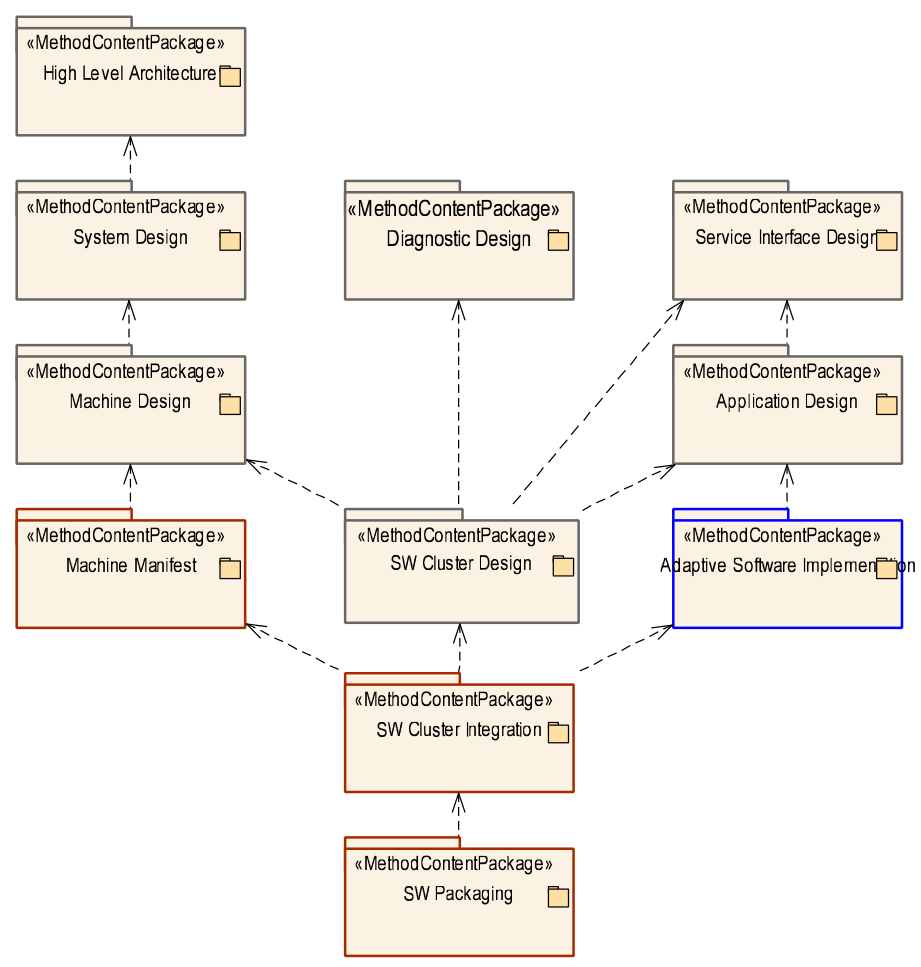
\includegraphics[width=0.75\textwidth]{Images/chap3/image_methodology/knowledgeBase/AdaptiveMethodology.png}
    \vspace{0.5cm}
    \caption{Adaptive Methodology}
    \label{fig:adap_methodology}
\end{figure}

% \subsubsection{High Level Architecture}

% % Figure before explanation
% \begin{figure}[H] % Dùng ht (here, top) là chuẩn nhất
%     \centering
%     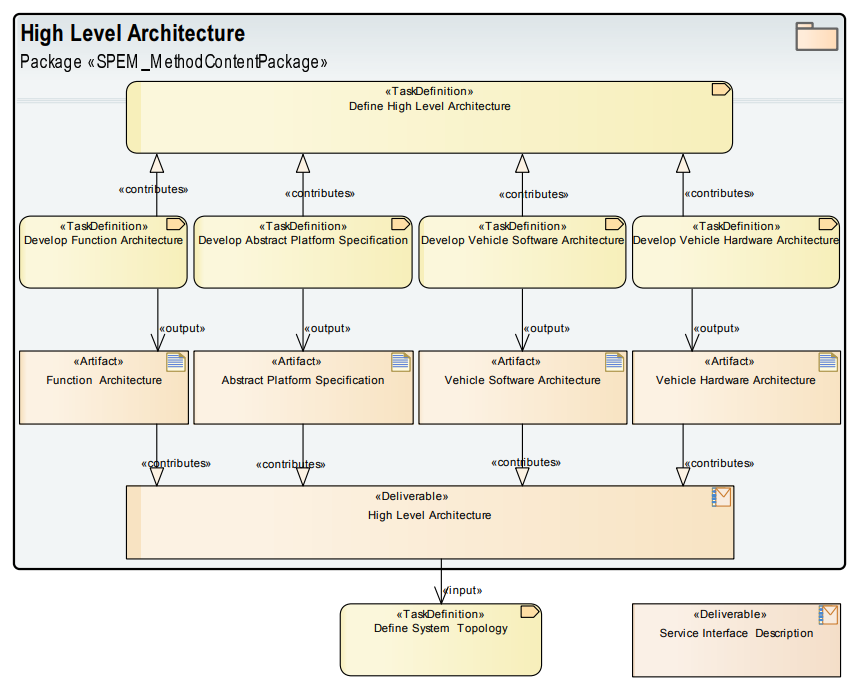
\includegraphics[width=0.75\textwidth]{Images/chap3/image_methodology/knowledgeBase/HLA.png}
%     \vspace{0.5cm}
%     \caption{High Level Architecture in Adaptive AUTOSAR Methodology}
%     \label{fig:hla_architecture} % Đã đổi tên nhãn để không trùng
% \end{figure}

% The High Level Architecture represents the initial and most abstract architectural view within the Adaptive AUTOSAR Methodology. Its primary purpose is to establish a common architectural foundation for the vehicle E/E system before detailed system design and implementation activities are performed.

% As illustrated in Figure~\ref{fig:hla_architecture}, the High Level Architecture is defined through a set of coordinated architectural tasks that collectively contribute to a unified architectural deliverable. These tasks include the development of the Function Architecture, the Abstract Platform Specification, the Vehicle Software Architecture, and the Vehicle Hardware Architecture. Each task addresses a specific architectural concern while remaining independent of concrete implementation decisions.

% The Function Architecture focuses on identifying and structuring the system functions and their logical relationships. It describes what the system is expected to do, without specifying how or where these functions are executed. In parallel, the Abstract Platform Specification defines the abstract execution environment and platform capabilities required by the software, serving as a conceptual bridge between functional requirements and platform realization.

% The Vehicle Software Architecture describes the high level organization of software elements within the vehicle, including major software partitions and their responsibilities. Complementarily, the Vehicle Hardware Architecture captures the high-level hardware structure of the system, including computing units and their relationships, without binding the architecture to specific hardware components.

% The outputs of these architectural tasks are formalized as architectural artefacts. These artefacts collectively contribute to the High-Level Architecture deliverable, which serves as a key input for subsequent methodology phases. In particular, the High Level Architecture provides the architectural context required for defining the system topology and service interface descriptions in later stages.

% By separating functional, software, hardware, and platform concerns at this early stage, the High Level Architecture supports architectural clarity, scalability, and consistency. It ensures that subsequent design and integration activities are grounded in a coherent and well-structured architectural vision.


% \subsubsection{System Design}

% % Figure before explanation
% \begin{figure}[H] % Dùng ht (here, top) là chuẩn nhất
%     \centering
%     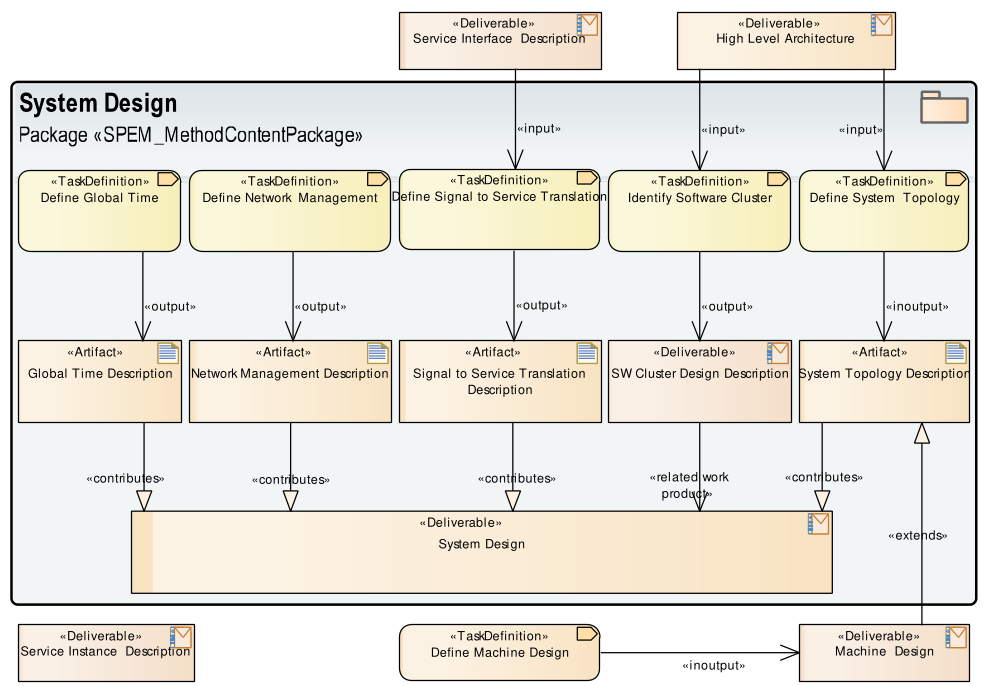
\includegraphics[width=0.75\textwidth]{Images/chap3/image_methodology/knowledgeBase/systemDesign.png}
%     \vspace{0.5cm}
%     \caption{System Design in Adaptive AUTOSAR Methodology}
%     \label{fig:system_design} % Đã đổi tên nhãn để không trùng
% \end{figure}

% The System Design phase refines the architectural concepts established in the High-Level Architecture into a more concrete and structured system-level description. Its primary objective is to define how software elements, communication mechanisms, and system resources are organized and coordinated within the Adaptive AUTOSAR environment.

% As illustrated in the System Design package, this phase consumes key architectural deliverables, including the High Level Architecture and the Service Interface Description, as inputs. Based on these inputs, a set of dedicated design tasks is performed to derive detailed system artefacts that collectively form the System Design deliverable.

% One of the central tasks in this phase is the definition of global timing concepts. The \textit{Define Global Time} task establishes a common time base for the system, which is essential for coordinating distributed software execution and ensuring temporal consistency across different system elements. The resulting Global Time Description contributes to the overall System Design by providing a unified temporal reference.

% In parallel, the \textit{Define Network Management} task specifies how communication networks are controlled and supervised at the system level. This task produces the Network Management Description, which defines network states, transitions, and management strategies. These definitions support reliable communication and controlled system behavior during startup, operation, and shutdown phases.

% Another key task within this phase is the \textit{Define Signal to Service Translation}. This task addresses the mapping between signal-oriented communication and service-oriented communication. The resulting Signal to Service Translation Description enables interaction between system elements that rely on different communication paradigms, ensuring compatibility and interoperability within the Adaptive Platform.

% The System Design phase also includes the identification of software clusters through the \textit{Identify Software Cluster} task. Software clusters group related software elements into coherent deployment units. The resulting Software Cluster Design Description serves as an important intermediate artefact that supports later integration and deployment activities.

% Furthermore, the \textit{Define System Topology} task specifies how system elements are arranged and connected. The System Topology Description captures function groups, network endpoints, and their relationships. This description provides a structural view of the system and serves as a foundation for subsequent deployment and machine-specific design steps.

% All artefacts generated during these tasks contribute to the System Design deliverable. Together, they establish a consistent and detailed system level specification that bridges the gap between high level architectural concepts and later design phases. The System Design deliverable also provides essential inputs for related activities, such as service instance specification and machine design.

% By consolidating timing, communication, clustering, and topology aspects, the System Design phase ensures that the Adaptive AUTOSAR system is coherently structured and ready for further refinement in subsequent methodology stages.


% % TODO: Insert system topology and communication overview figure

% \subsubsection{Service Interface Design}

% % Figure before explanation
% \begin{figure}[H] % Dùng ht (here, top) là chuẩn nhất
%     \centering
%     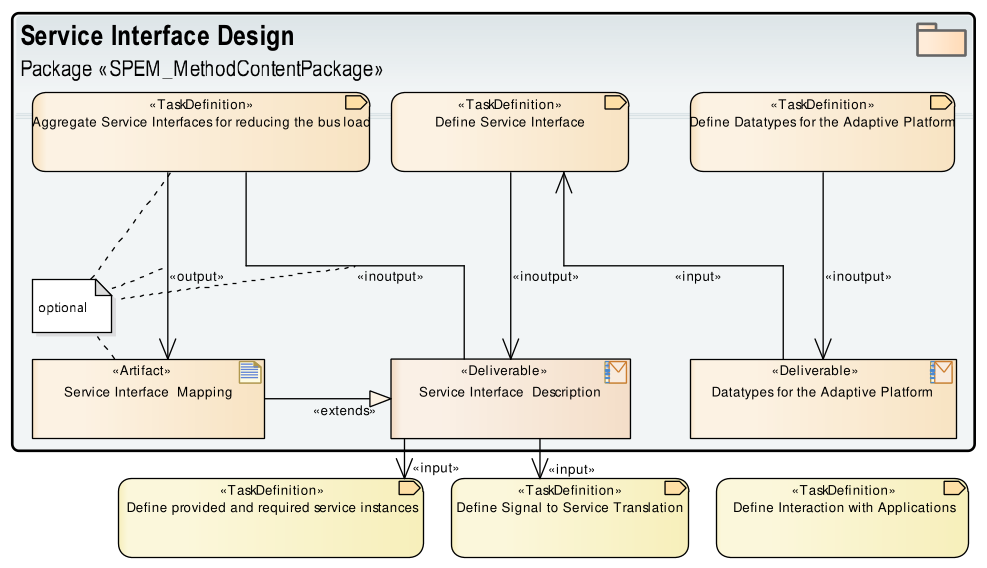
\includegraphics[width=0.75\textwidth]{Images/chap3/image_methodology/knowledgeBase/serviceInterfaceDesign.png}
%     \vspace{0.5cm}
%     \caption{Service Interface Design in Adaptive AUTOSAR Methodology}
%     \label{fig:service_interface_design} % Đã đổi tên nhãn để không trùng
% \end{figure}

% The Service Interface Design defines how Service Interface Descriptions are created, refined, and reused within the Adaptive AUTOSAR development process. This usage scenario explains the sequence of design activities and their associated work products, as illustrated in Figure~\ref{fig:service_interface_design}, focusing on the relationship between service interfaces, datatypes, and interface mappings.

% According to the methodology, Service Interface Descriptions can be obtained through two main usage scenarios: create or change use cases and reuse use cases. These scenarios are not isolated phases but can be integrated into both system design and application design activities, depending on the development context.

% In create or change use cases, Service Interface Descriptions are derived by performing a set of tailored tasks. The central task is the definition of a service interface, which specifies the service operations, events, and communication semantics. In parallel, datatypes for the Adaptive Platform are defined or refined to describe the data exchanged through the service interface. These tasks may be supported by the aggregation of service interfaces, which aims to reduce communication bus load by grouping related service elements when appropriate. The resulting Service Interface Mapping artefact optionally extends the Service Interface Description by documenting how aggregated or related interfaces are organized.

% This scenario is typically applied in a top-down development approach, where architectural or system level considerations drive the definition of service interfaces and datatypes. The outputs of these tasks include the Service Interface Description and the Datatypes for the Adaptive Platform, which together form the primary deliverables of this design stage.

% In reuse use cases, existing Service Interface Descriptions are adopted as inputs with minimal modification. In this case, service interfaces and their associated datatypes are reused from predefined specifications or existing libraries. If required, datatypes may be extended to align with the specific system context. This scenario is commonly applied in a bottom-up development approach and supports efficient reuse across different projects.

% The resulting work products of both scenarios are tailored Service Interface Descriptions and corresponding Datatype Descriptions. These deliverables serve as inputs for subsequent design activities, such as the definition of provided and required service instances, signal-to-service translation, and the specification of interactions with applications.

% By explicitly structuring the creation, aggregation, mapping, and reuse of service interfaces, the Service Interface Design usage scenario ensures consistency, modularity, and reusability of service definitions within the Adaptive AUTOSAR methodology.

% \subsubsection{Application Design}

% % Figure before explanation
% \begin{figure}[H]
%     \centering
%     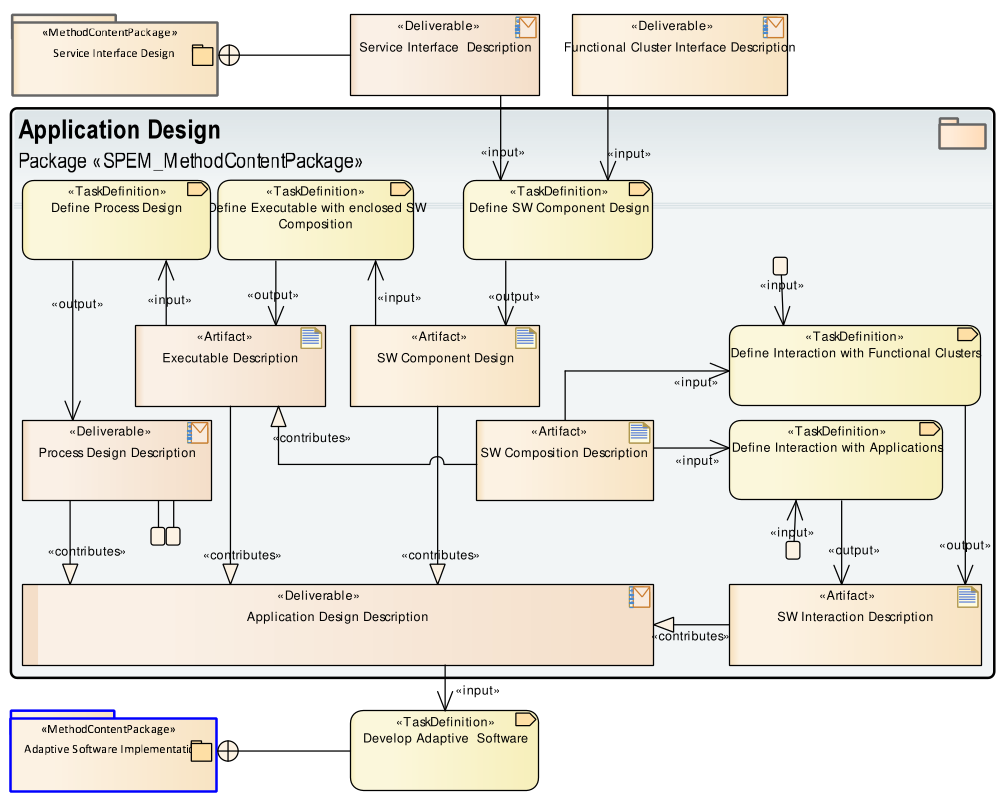
\includegraphics[width=0.75\textwidth]{Images/chap3/image_methodology/knowledgeBase/applicationDesign.png}
%     \vspace{0.5cm}
%     \caption{Application Design in Adaptive AUTOSAR Methodology}
%     \label{fig:application_design}
% \end{figure}

% The Application Design phase refines the outcomes of system level and service-level design into a detailed specification of executable software structures. Its primary objective is to describe how software components are organized, instantiated, and interconnected during runtime execution within the Adaptive AUTOSAR Platform.

% As shown in Figure~\ref{fig:application_design}, this phase takes the Service Interface Description and the Functional Cluster Interface Description as inputs. Based on these artefacts, a set of closely related design activities is carried out, leading to the definition of the overall Application Design Description.

% One of the key activities in this phase is \textit{Define Software (SW) Component Design}. This activity results in the SW Component Design artefact, which specifies the internal structure of software components and their interaction endpoints. These endpoints are expressed through software component (SWC) ports instantiating specific port interfaces at either the application level or the platform level. The SW Component Design establishes the structural basis required for subsequent composition and interaction definitions.

% Another essential activity is \textit{Define Executable with enclosed SW Composition}, which determines how software components are assembled into executable units. Its outcome is the Executable Description, including the SW Composition Description. This description identifies the software components contained within an executable and defines their structural relationships. The execution of this activity requires that all referenced SW Component Designs are already available.

% The runtime realization of executables is addressed by the \textit{Define Process Design} activity. The resulting Process Design Description represents a design time abstraction of the operating system process responsible for instantiating and starting a specific executable. This activity builds upon the Executable Description and provides the link between executable definitions and their runtime execution context.

% Interaction which related aspects are specified through the activities \textit{Define Interaction with Applications} and \textit{Define Interaction with Functional Clusters}. Together, these activities produce the SW Interaction Description, which captures all interaction configurations that are relevant at design time. This includes interactions between application-level software components as well as interactions with platform-level functional clusters. The definition of these interactions depends on the availability of the Process Design Description, the corresponding Executable Description with its SW Composition Description, and the interaction endpoints defined in the SW Component Designs.

% All artefacts produced during the Application Design phase contribute to the Application Design Description deliverable. This deliverable consolidates software component definitions, executable compositions, process abstractions, and interaction configurations into a consistent and comprehensive design representation.

% The activities within the Application Design phase are interdependent and may be performed in an order that best fits the project context. Although the primary focus of this phase is on application-level software, the same design principles and activities may also be applied to platform-level software, particularly when port and port interface concepts are supported.

% The resulting Application Design Description serves as a fundamental input for the subsequent Adaptive Software Implementation phase, where the defined software structures are realized as executable software.

% \subsubsection{Adaptive Software Implementation}

% % Figure before explanation
% \begin{figure}[H]
%     \centering
%     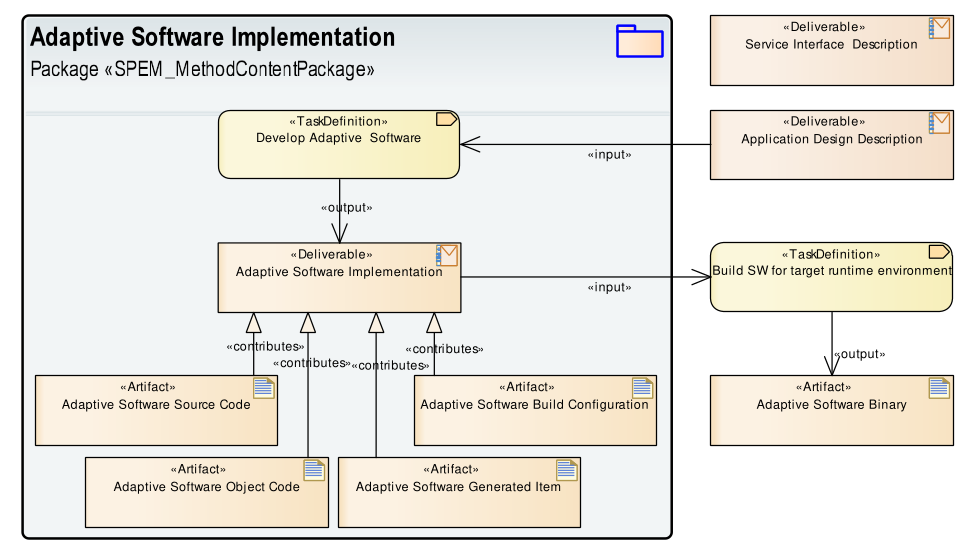
\includegraphics[width=0.75\textwidth]{Images/chap3/image_methodology/knowledgeBase/softwareImplementation.png}
%     \vspace{0.5cm}
%     \caption{Adaptive Software Implementation in Adaptive AUTOSAR Methodology}
%     \label{fig:software_implementation}
% \end{figure}

% The Adaptive Software Implementation phase addresses the realization of software defined during the preceding design stages. Its purpose is to transform the Application Design Description into concrete software artefacts that can be integrated and executed within the Adaptive AUTOSAR runtime environment.

% As depicted in Figure~\ref{fig:software_implementation}, this phase is initiated once the Service Interface Description and the Application Design Description are available. These deliverables provide the necessary interface definitions and structural specifications required to start the implementation activities.

% The central activity of this phase is \textit{Develop Adaptive Software}. This activity encompasses the development of application level and/or platform level Adaptive Software and may include analysis, detailed design, implementation, and testing activities. The development process relies on Adaptive Software Generated Items, such as service proxies and service skeletons, which are derived from service interface definitions and support the implementation of communication ports and port interfaces.

% Depending on the availability of the Adaptive Software Build Configuration, the development process follows different realization paths. When the build configuration is known in advance, software components can be compiled by the developer, and Adaptive Software Object Code can be delivered directly. In contrast, if the build configuration is not available, the developer provides Adaptive Software Source Code, and the compilation is performed later by the integrator.

% The artefacts produced during software development include Adaptive Software Source Code, Adaptive Software Object Code, Adaptive Software Generated Items, and the Adaptive Software Build Configuration. Together, these artefacts contribute to the Adaptive Software Implementation deliverable, which represents the complete implementation result prepared for integration.

% The transformation of the implementation into deployable form is addressed by the activity \textit{Build software (SW) for target runtime environment}. This activity consumes the Adaptive Software Implementation and produces the Adaptive Software Binary. The binary represents the executable form of the software that is suitable for deployment on the target machine and runtime environment.

% Throughout this phase, both application level and platform level Adaptive Software are treated consistently. Each executable requires a main function and an execution manifest, enabling instantiation and deployment within the Adaptive AUTOSAR execution framework.

% The Adaptive Software Implementation deliverable produced in this phase serves as the handover point between software development and integration. It provides the necessary implementation artefacts for subsequent software cluster integration, packaging, and deployment activities.

% \subsubsection{Diagnostic Design}

% % Figure before explanation
% \begin{figure}[H]
%     \centering
%     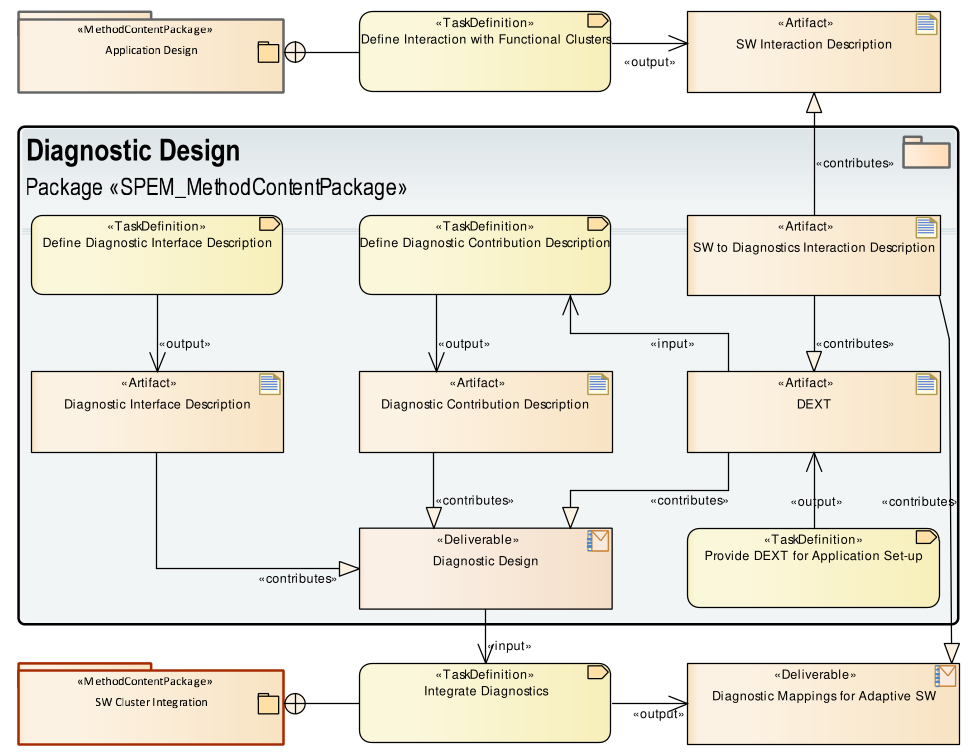
\includegraphics[width=0.75\textwidth]{Images/chap3/image_methodology/knowledgeBase/diagDesign.png}
%     \vspace{0.5cm}
%     \caption{Diagnostic Design in Adaptive AUTOSAR Methodology}
%     \label{fig:diag_design}
% \end{figure}

% The Diagnostic Design phase focuses on defining how diagnostic information is associated with the software structures of the Adaptive AUTOSAR system. Its main objective is to prepare diagnostic which related artefacts that enable consistent monitoring, reporting, and interaction with the diagnostic manager during system operation.

% As shown in Figure~\ref{fig:diag_design}, Diagnostic Design builds on results obtained during the Application Design phase, particularly the SW Interaction Description that captures interactions with functional clusters. These interaction definitions provide the context required to specify diagnostic interfaces and mappings in a systematic manner.

% The activity \textit{Define Diagnostic Interface Description} establishes the diagnostic interfaces that adaptive software components expose for diagnostic purposes. The resulting Diagnostic Interface Description specifies diagnostic port interfaces and their characteristics, allowing diagnostic managers to access diagnostic which relevant data and services in a standardized way.

% Complementing this, the activity \textit{Define Diagnostic Contribution Description} identifies the diagnostic content contributed by software elements within a given context. The Diagnostic Contribution Description determines which parts of the diagnostic configuration are relevant for specific executables or software clusters and are intended to be processed by the diagnostic manager.

% Diagnostic resources and configuration data are collected and structured through the activity \textit{Provide DEXT for Application Setup}. This activity produces or extends the Diagnostic Extract (DEXT), which contains diagnostic resources such as diagnostic data identifiers, diagnostic events, enable conditions, and operation cycles. The DEXT acts as a reusable container for diagnostic configuration and may cover multiple executables, diagnostic managers, and software clusters across the vehicle.

% The association between diagnostic resources and software interaction endpoints is captured in the SW to Diagnostics Interaction Description. This artefact specifies how diagnostic information is mapped to software component ports at design time and contributes both to the Diagnostic Design deliverable and to the DEXT. It represents an intermediate form of diagnostic mappings that is refined during later integration steps.

% All artefacts produced during this phase, including the Diagnostic Interface Description, Diagnostic Contribution Description, SW to Diagnostics Interaction Description, and the DEXT, collectively contribute to the Diagnostic Design deliverable. This deliverable provides a consolidated view of the diagnostic configuration that is prepared for further integration activities.

% The Diagnostic Design deliverable is subsequently used as input for the \textit{Integrate Diagnostics} activity during Software Cluster Integration. In that phase, diagnostic mappings are finalized by associating diagnostic resources with concrete executable instances and operating system processes, resulting in the Diagnostic Mappings for Adaptive Software.

% By structuring diagnostic interface definition, contribution specification, and resource extraction as distinct but related activities, the Diagnostic Design phase supports a clear and maintainable diagnostic configuration process within the Adaptive AUTOSAR methodology.

% \subsubsection{Machine Design}

% % Figure before explanation
% \begin{figure}[H]
%     \centering
%     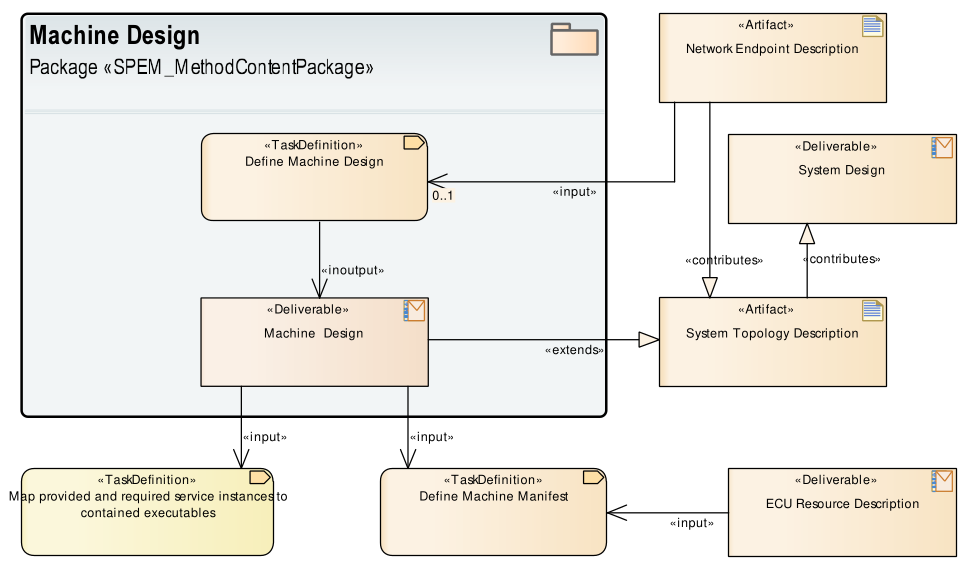
\includegraphics[width=0.75\textwidth]{Images/chap3/image_methodology/knowledgeBase/machineDesign.png}
%     \vspace{0.5cm}
%     \caption{Machine Design in Adaptive AUTOSAR Methodology}
%     \label{fig:machine_design}
% \end{figure}

% The Machine Design phase addresses the specification of a machine from a communication and deployment standpoint within the Adaptive AUTOSAR Platform. Its aim is to describe the characteristics of a machine that are required for software execution and service communication, taking into account system level topology information and the capabilities of the target ECU.

% Figure~\ref{fig:machine_design} provides an overview of the activities involved in this phase. The core activity, \textit{Define Machine Design}, derives a machine-oriented configuration by using network endpoint information defined during System Design. In particular, the System Topology Description and the associated Network Endpoint Description supply the addressing and service discovery parameters needed to shape the communication behavior of the machine.

% The result of this activity is captured in the Machine Design deliverable. This deliverable augments the existing System Topology Description by introducing machine specific communication constraints and requirements. At this stage, the design remains independent of a concrete hardware realization and represents a prospective configuration for a machine.

% Beyond defining communication aspects, the Machine Design also provides the basis for associating software deployment elements with the machine. Through the activity \textit{Map provided and required service instances to contained executables}, service instances are linked to executables that are intended to run on the machine. This association clarifies how services are realized by software units within the machine context.

% The adaptation of the machine configuration to a specific hardware platform is performed in a subsequent activity, \textit{Define Machine Manifest}. This activity combines the Machine Design with the ECU Resource Description, which details the resources and limitations of the target ECU. The outcome is the Machine Manifest, representing a machine configuration that is fully aligned with the characteristics of a real ECU.

% From a methodological viewpoint, machine configuration follows a two-step process. The first step establishes the communication structure of a machine and yields the Machine Design. This step may be carried out in a top-down manner, guided by an existing System Design, or in a bottom-up manner, where machine-specific communication definitions are created locally and may later contribute to the overall system topology.

% The second step focuses on hardware-specific realization and results in the Machine Manifest. This separation between prospective machine definition and ECU specific configuration supports a clear allocation of responsibilities between system designers and integrators, while maintaining flexibility during system integration.

% \subsubsection{Machine Manifest}

% % Figure before explanation
% \begin{figure}[H]
%     \centering
%     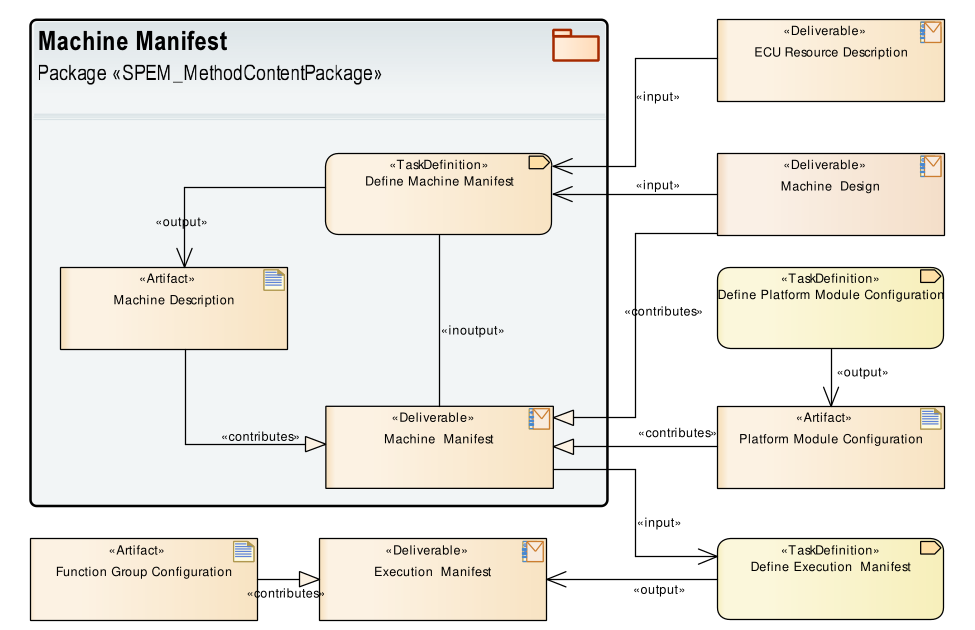
\includegraphics[width=0.75\textwidth]{Images/chap3/image_methodology/knowledgeBase/machineManifest.png}
%     \vspace{0.5cm}
%     \caption{Machine Manifest in Adaptive AUTOSAR Methodology}
%     \label{fig:machine_manifest}
% \end{figure}

% The Machine Manifest phase specifies the final configuration of a machine that is ready to be deployed on a concrete ECU within the Adaptive AUTOSAR Platform. Its purpose is to consolidate communication-related design results with hardware resource information and platform-specific configurations into a single, deployment ready description.

% Figure~\ref{fig:machine_manifest} outlines the activities and work products involved in this phase. The primary activity, \textit{Define Machine Manifest}, is initiated once the Machine Design and the ECU Resource Description are available. While the Machine Design provides a prospective view of the machine configuration, the ECU Resource Description defines the concrete hardware resources offered by the target ECU.

% The outcome of this activity is the Machine Manifest deliverable. The Machine Manifest integrates several key elements. First, it contains the Machine Description, which describes the available hardware resources of the ECU, such as processing units, memory resources, sensors, actuators, and other relevant hardware elements. This information is derived from the ECU Resource Description and tailored to the specific machine instance.

% Second, the Machine Manifest incorporates the Machine Design, thereby preserving the communication structure and network-related configuration that was defined during the Machine Design phase. This ensures that the communication requirements identified earlier are consistently realized on the target ECU.

% In addition, platform-specific aspects are addressed through the activity \textit{Define Platform Module Configuration}. This activity produces Platform Module Configuration artefacts, which specify the machine-specific configuration of Adaptive Platform modules. These configurations may include the operating system setup, platform services such as network management and diagnostics, as well as foundation modules like logging and tracing. The resulting Platform Module Configurations contribute directly to the Machine Manifest.

% The configuration of software execution is captured by the activity \textit{Define Execution Manifest}. This activity produces the Execution Manifest, which specifies which executables are instantiated on the machine and how they are mapped to processes. The Execution Manifest may also include Function Group Configurations that control the activation and deactivation of software elements. The Execution Manifest contributes to the Machine Manifest by defining the runtime behavior of software on the machine.

% From a process perspective, the Machine Manifest is typically assembled in an incremental manner. Communication-related configurations originating from the Machine Design are collected first, followed by the integration of hardware resource descriptions and platform module configurations. As additional configuration information becomes available, the Machine Manifest may be iteratively extended and refined.

% By consolidating machine-specific communication settings, hardware resource descriptions, platform module configurations, and execution information, the Machine Manifest provides a complete and consistent representation of a machine that is ready for deployment within the Adaptive AUTOSAR ecosystem.

% \subsubsection{Software Cluster Design, Integration, and Packaging}

% The phases of Software Cluster Design, Software Cluster Integration, and Software Packaging together form the final preparation steps that transform implemented Adaptive AUTOSAR software into deployable units. These phases consolidate design results, integrate software components with their configurations, and prepare complete software packages for deployment on target machines.

% Software Cluster Design focuses on defining logical groupings of software elements that belong together from a deployment and lifecycle perspective. A software cluster typically bundles application level software, required platform services, and related configuration artifacts into a coherent unit. The purpose of this phase is not to define execution details, but to establish clear cluster boundaries, dependencies, and responsibilities that simplify later integration and deployment activities.

% Based on the cluster definitions, Software Cluster Integration performs the concrete assembly of software and configuration artifacts. During this phase, Adaptive Software Implementations, design descriptions, machine which related information, and diagnostic configurations are brought together and checked for consistency. Integration activities refine execution which related information, such as the association of executables with machines and processes, and complete interaction and diagnostic mappings that could only be finalized once all involved elements are known. As a result, the integrated software cluster represents a consistent and executable view of the system for a specific deployment context.

% Software Packaging completes the workflow by preparing integrated software clusters for delivery and deployment. In this phase, all relevant artifacts, such as software binaries, manifests, configuration files and generated items which are collected and organized into software packages. These packages are structured in a way that supports deployment, update, and lifecycle management, while preserving a clear separation between different software clusters.

% By combining cluster definition, integration, and packaging into a structured workflow, these phases provide a clear transition from implemented software to deployable units. This approach supports modularity, reuse, and scalable integration, which are essential characteristics of the Adaptive AUTOSAR methodology.

% \subsubsection{Summary}

% This section has presented an overview of the Adaptive AUTOSAR knowledge base and its role in structuring the development of complex automotive software systems. The methodology defines a clear sequence of development phases, each supported by well-defined artefacts and responsibilities.

Starting from high-level architectural descriptions, the methodology guides the refinement of system structure, service interfaces, application design, and software implementation. Subsequent phases address diagnostics, machine-specific configuration, and the preparation of software for deployment. Each phase builds upon the results of previous stages, ensuring consistency and traceability throughout the development process.

By explicitly modeling artefact dependencies and separating design, implementation, integration, and deployment concerns, the Adaptive AUTOSAR Methodology supports systematic system development. This approach improves scalability, facilitates reuse, and simplifies integration in large and evolving software systems.

The following section explains how the most important Method Content Packages are configured in this project and how they are refined into concrete Adaptive AUTOSAR artefacts.

% Overall, the knowledge base provides a solid methodological foundation for configuring and deploying Adaptive AUTOSAR systems. It enables a structured transition from abstract system concepts to deployable software units while maintaining clarity and consistency across the entire system lifecycle.


\subsection{Project Methodology}

In this project, the Adaptive AUTOSAR system is developed using the \texttt{Autosar.io} tool provided by PopcornSAR. Autosar.io is a configuration-oriented modeling environment that allows users to systematically define and organize an Adaptive AUTOSAR project through a set of well-structured design sections. Instead of focusing on source code implementation, the tool guides users to configure machines, services, and applications by following the standard Adaptive AUTOSAR modeling workflow.

\begin{figure}[H]
    \centering
    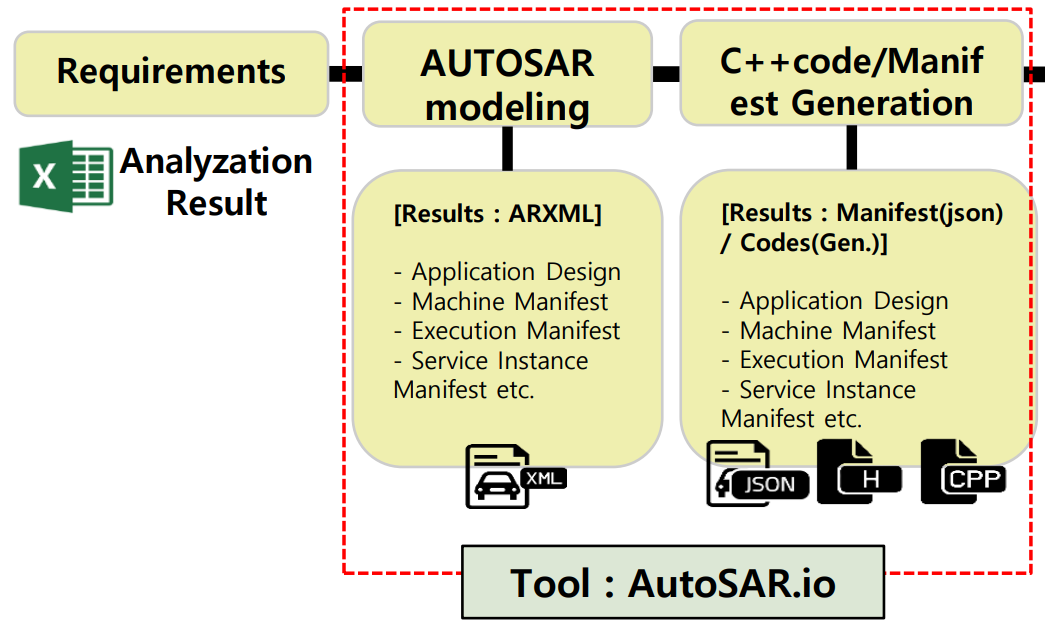
\includegraphics[width=0.75\textwidth]{Images/toolchains/autosario.png}
    \vspace{0.5cm}
    \caption{Autosar.io tool supporting configuration workflow for Adaptive AUTOSAR systems}
    \label{fig:autosario}
\end{figure}

Autosar.io provides dedicated design views that correspond directly to the configuration steps presented in this section, including Machine Design and Machine Manifest creation, Service Interface Design and Mapping, and Adaptive Application Design. Through these views, users can specify network endpoints, service discovery parameters, service interfaces, service instances, application executables, processes, startup behavior, and process-to-machine mappings. Each configuration step produces AUTOSAR-compliant artifacts such as ARXML descriptions and manifests, ensuring consistency between design intent and deployment configuration.

By using Autosar.io, users can incrementally build the system configuration in a top-down manner, where abstract architectural decisions are progressively refined into concrete runtime configurations. This approach enables clear separation between machine-level configuration, service-level communication design, and application-level deployment. As demonstrated throughout this section, Autosar.io acts as the central tool that connects all configuration stages, allowing users to define a complete Adaptive AUTOSAR system in a structured, traceable, and standardized way before moving to implementation and integration phases.

%introduce Autosar.io tool, this is a tool help configuring project based on Adaptive AUTOSAR
\subsubsection{High Level Architecture}
\begin{figure}[H]
    \centering
    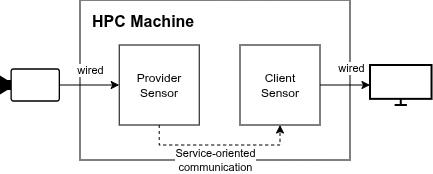
\includegraphics[width=0.75\textwidth]{Images/chap3/image_methodology/machineDesign/high_level.png}
    \vspace{0.5cm}
    \caption{High Level Architecture of Prototype Project}
    \label{fig:hla_project}
\end{figure}

Based on the defined high-level architecture, the Adaptive AUTOSAR configuration process is carried out in a stepwise manner, following the recommended methodology. The overall system design is progressively refined from an abstract architectural view to concrete deployment and execution artifacts.

First, the Machine Design and Machine Manifest are configured to define the physical execution environment of the system. This step specifies the target machine, network interfaces, service discovery settings, operating system platform modules, and lifecycle-related parameters, forming the foundation on which all applications and services are deployed.

Next, the Service Interface Design and Mapping phase focuses on defining the service-oriented communication between applications. During this stage, data types, service interfaces, service instances, and deployment configurations are specified, and abstract service definitions are bound to concrete network endpoints. This step enables standardized and loosely coupled interaction between the Provider Sensor and Client Sensor.

Finally, the Application Design phase models the adaptive applications themselves. Executables are defined and configured, ports are mapped to service interfaces, application processes are created, and startup and lifecycle behaviors are specified. Through this step, the logical application design is concretely mapped onto the target machine, completing the system configuration prior to code and manifest generation.

\subsubsection{Machine Design and Machine Manifest}

% Define Ethernet network endpoint
\begin{figure}[H]
    \centering
    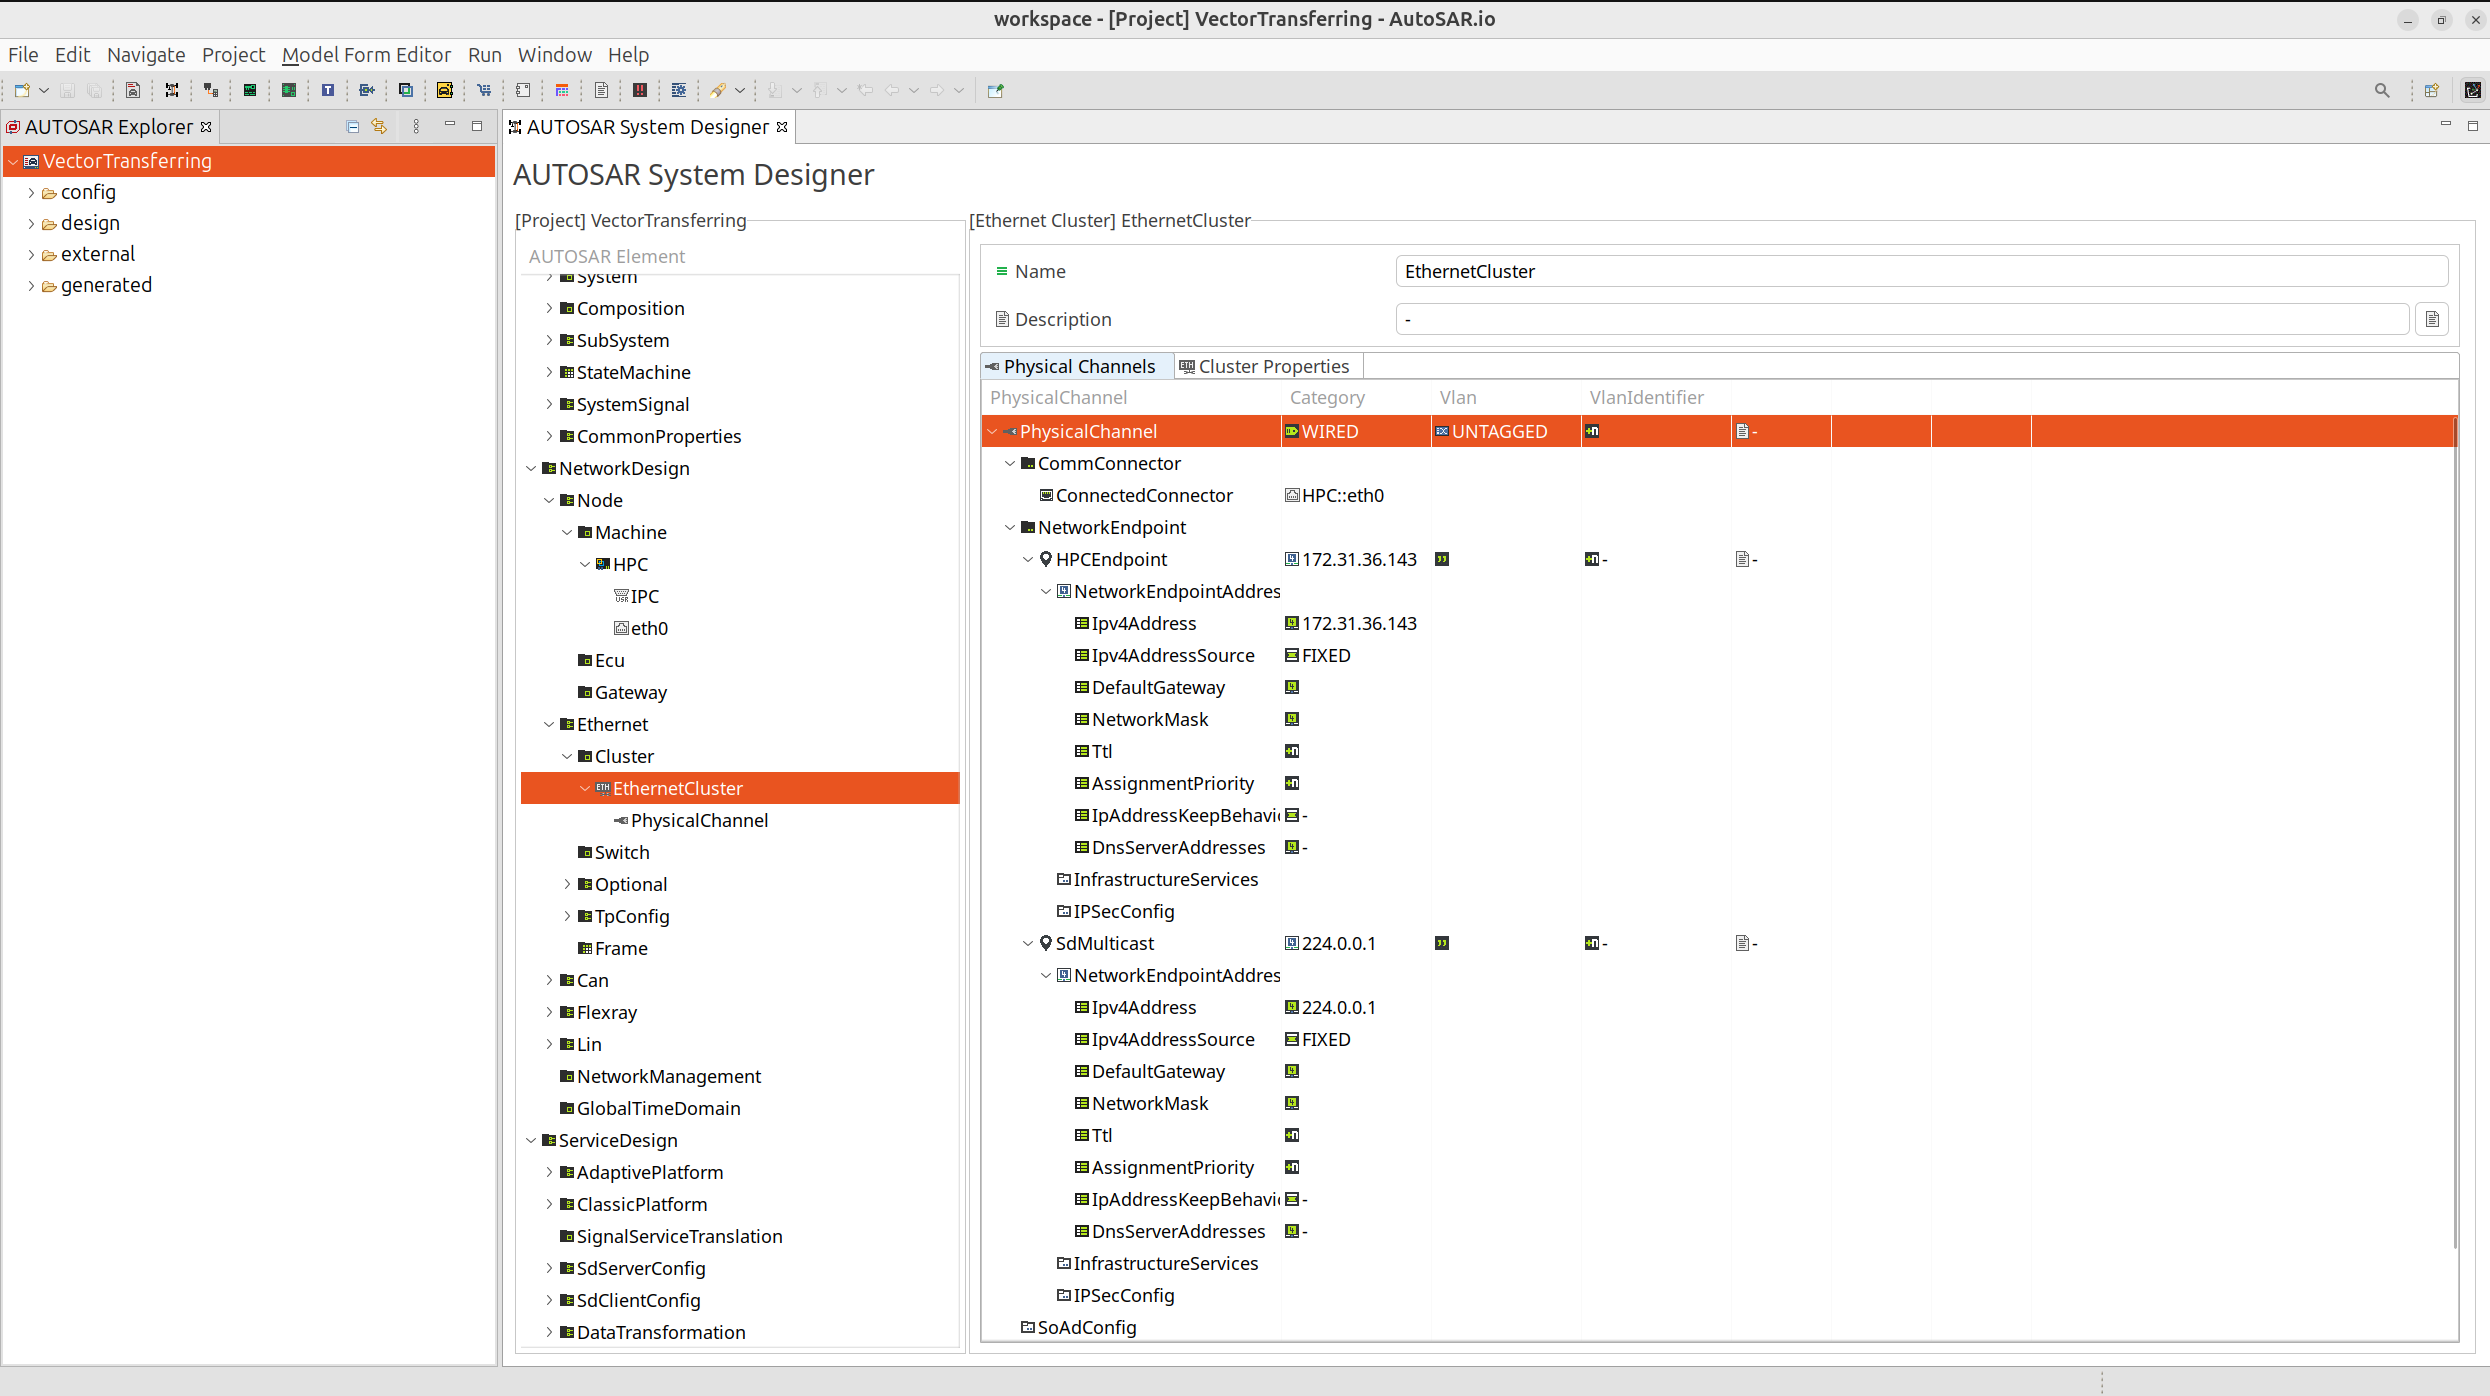
\includegraphics[width=0.75\textwidth]{Images/chap3/image_methodology/machineDesign/defineEthernet.png}
    \vspace{0.5cm}
    \caption{Definition of Ethernet Network Endpoint in Machine Design}
    \label{fig:machine_define_ethernet}
\end{figure}

Figure~\ref{fig:machine_define_ethernet} illustrates the detailed configuration of an Ethernet network endpoint within the AUTOSAR System Designer. An EthernetCluster is defined with a wired physical channel, where the VLAN mode is set to untagged, indicating that no VLAN identifier is applied to the network traffic. The machine node labeled HPC is connected to this cluster through the communication connector HPC eth0, which represents the physical Ethernet interface of the target machine.

The network endpoint configuration specifies a fixed IPv4 address of 172.31.36.143, with the address source explicitly defined as fixed to ensure deterministic network behavior. In addition to the unicast endpoint, a multicast configuration is also present using the IPv4 address 224.0.0.1, which is commonly used for service discovery communication. These settings collectively define how the machine participates in both point to point and multicast Ethernet communication, forming a stable networking foundation for Adaptive AUTOSAR service based applications.

% Add Ethernet configuration to Machine Design
\begin{figure}[H]
    \centering
    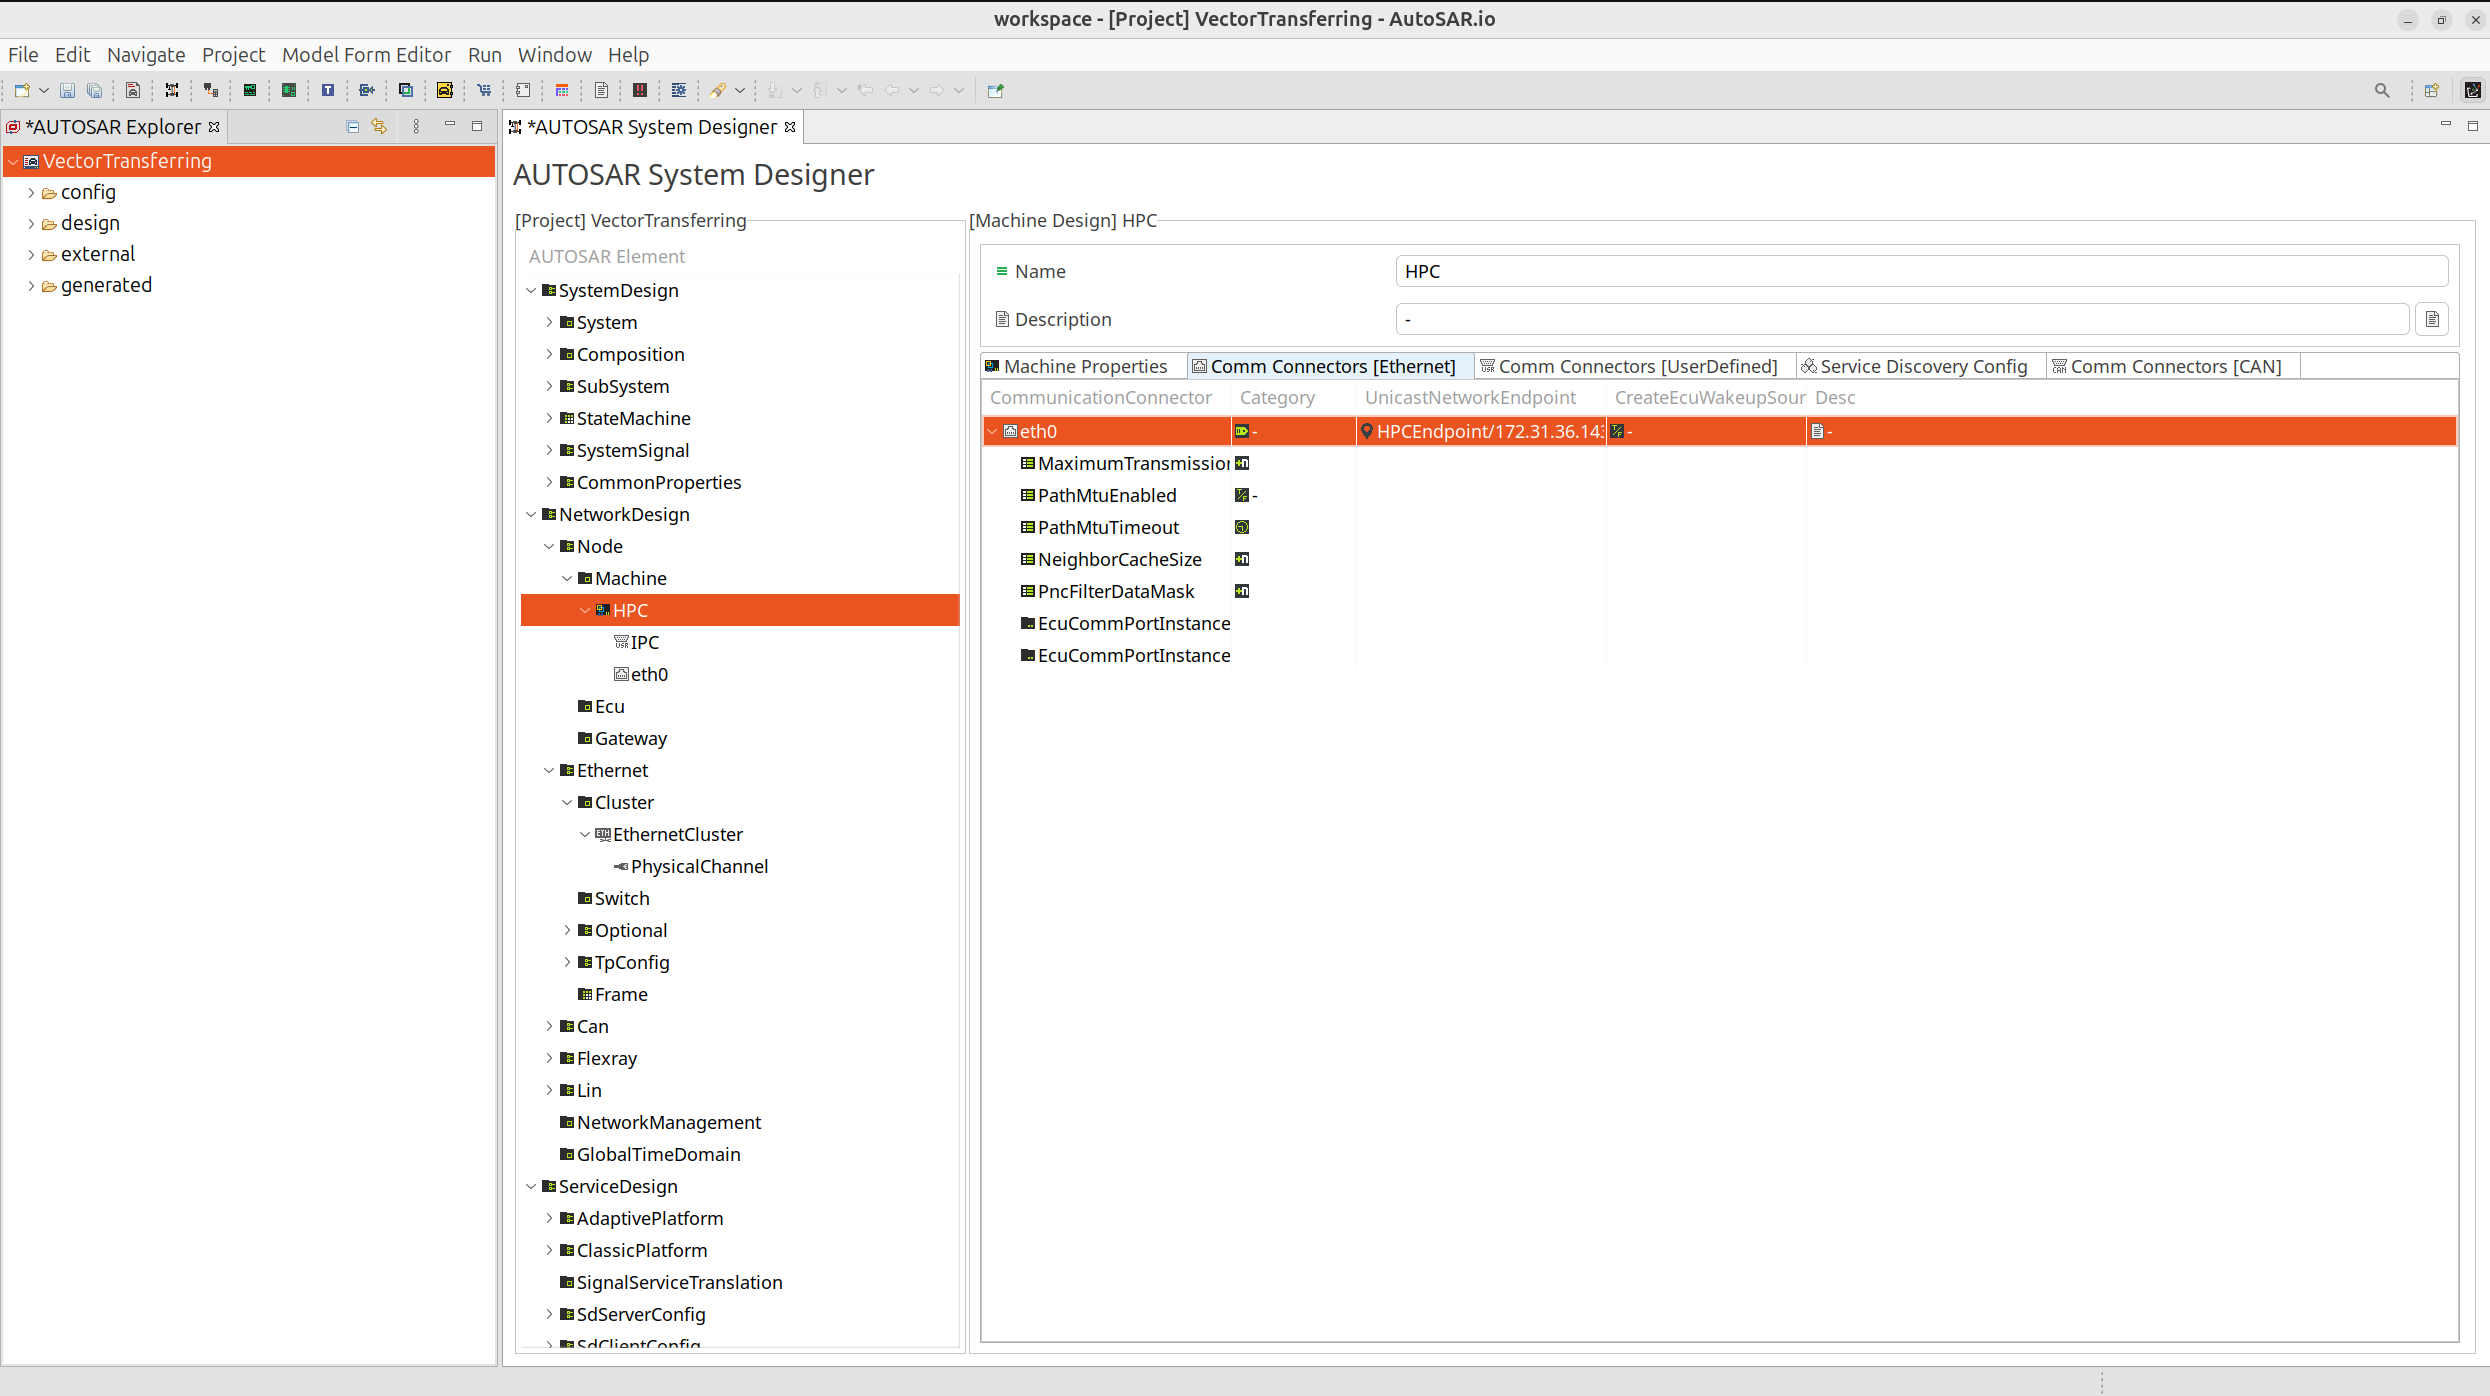
\includegraphics[width=0.75\textwidth]{Images/chap3/image_methodology/machineDesign/addEthMachineDesign.png}
    \vspace{0.5cm}
    \caption{Integration of Ethernet Configuration into Machine Design}
    \label{fig:machine_add_eth_design}
\end{figure}

Figure~\ref{fig:machine_add_eth_design} depicts how the HPC machine is linked to its network interface through the eth0 connector in the Machine Design view. This connector is mapped to a unicast endpoint identified as HPCEndpoint with the IPv4 address 172.31.36.143, defining the machine’s network presence within the Adaptive AUTOSAR system. The figure also highlights adjustable communication parameters such as transmission limits and path MTU handling, which allow the network behavior to be adapted while maintaining reliable data exchange at runtime.

% Configure Service Discovery in Machine Design
\begin{figure}[H]
    \centering
    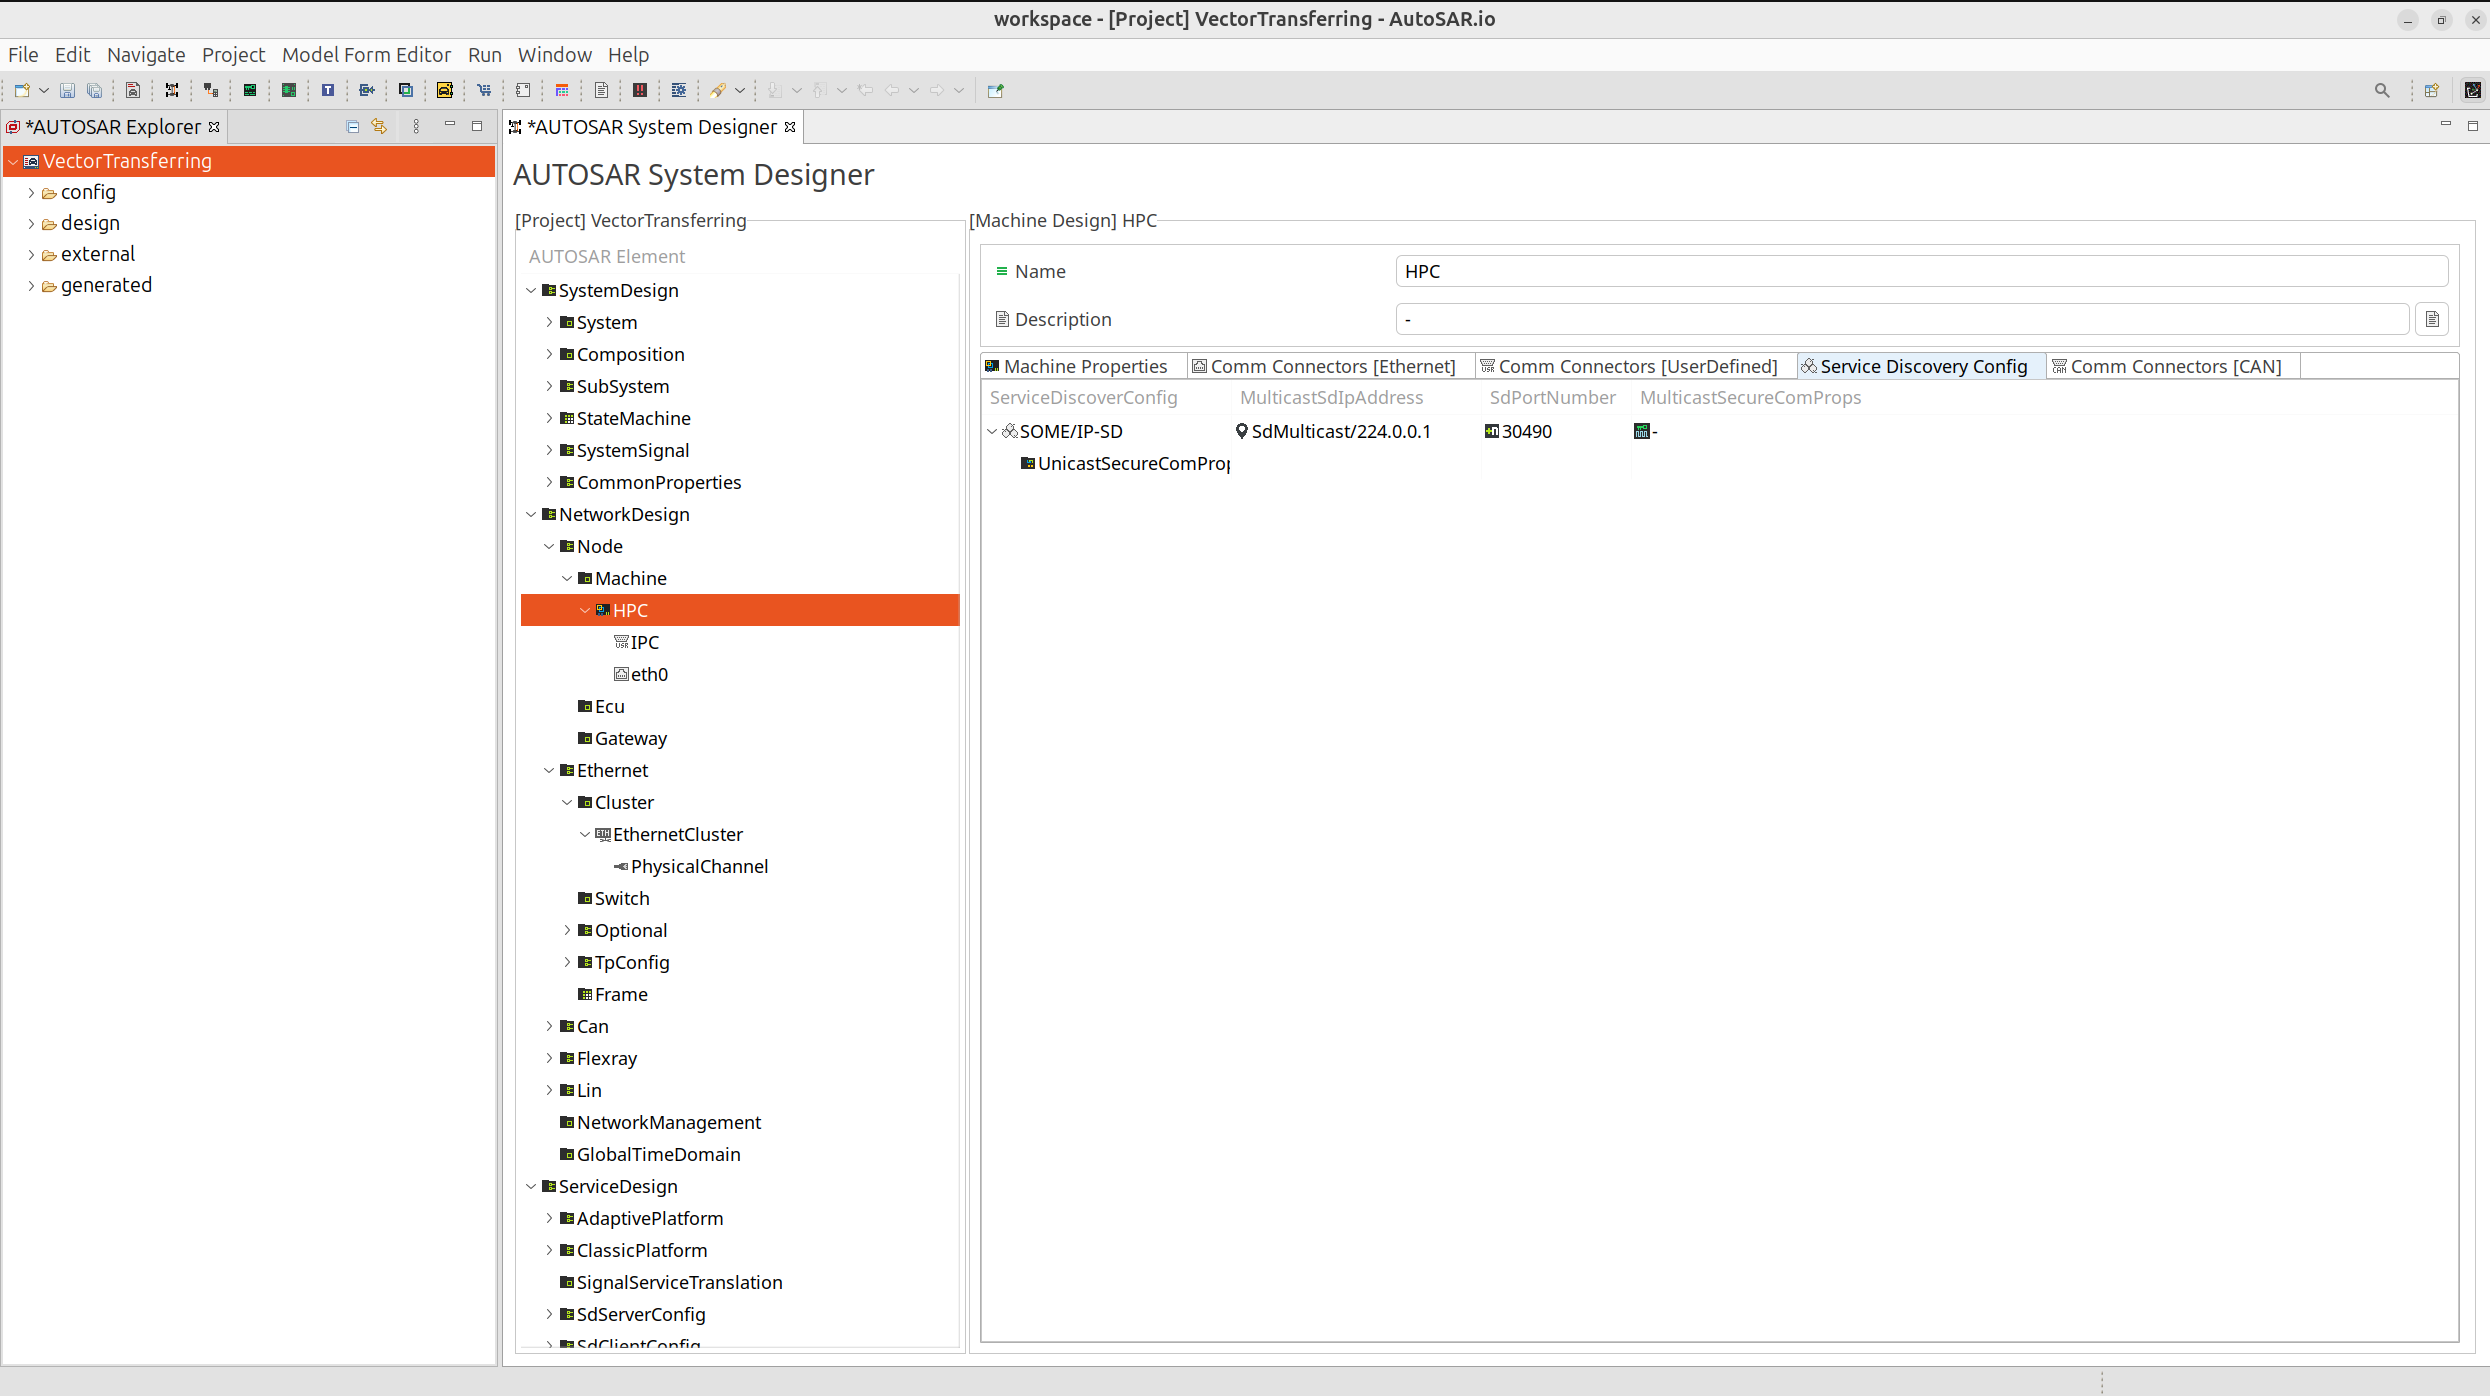
\includegraphics[width=0.75\textwidth]{Images/chap3/image_methodology/machineDesign/addSdConfigMachineDesign.png}
    \vspace{0.5cm}
    \caption{Service Discovery Configuration in Machine Design}
    \label{fig:machine_sd_config}
\end{figure}

Figure~\ref{fig:machine_sd_config} illustrates the Service Discovery setup for the HPC machine within the Machine Design environment. The SOME IP Service Discovery mechanism is configured using the multicast address 224.0.0.1 together with the service discovery port number 30490, which enables applications to announce and detect available services at runtime. This configuration allows dynamic interaction between Adaptive AUTOSAR applications while supporting flexible service availability without relying on static communication bindings.

% Configure Diagnostic Log and Trace (DLT)
\begin{figure}[H]
    \centering
    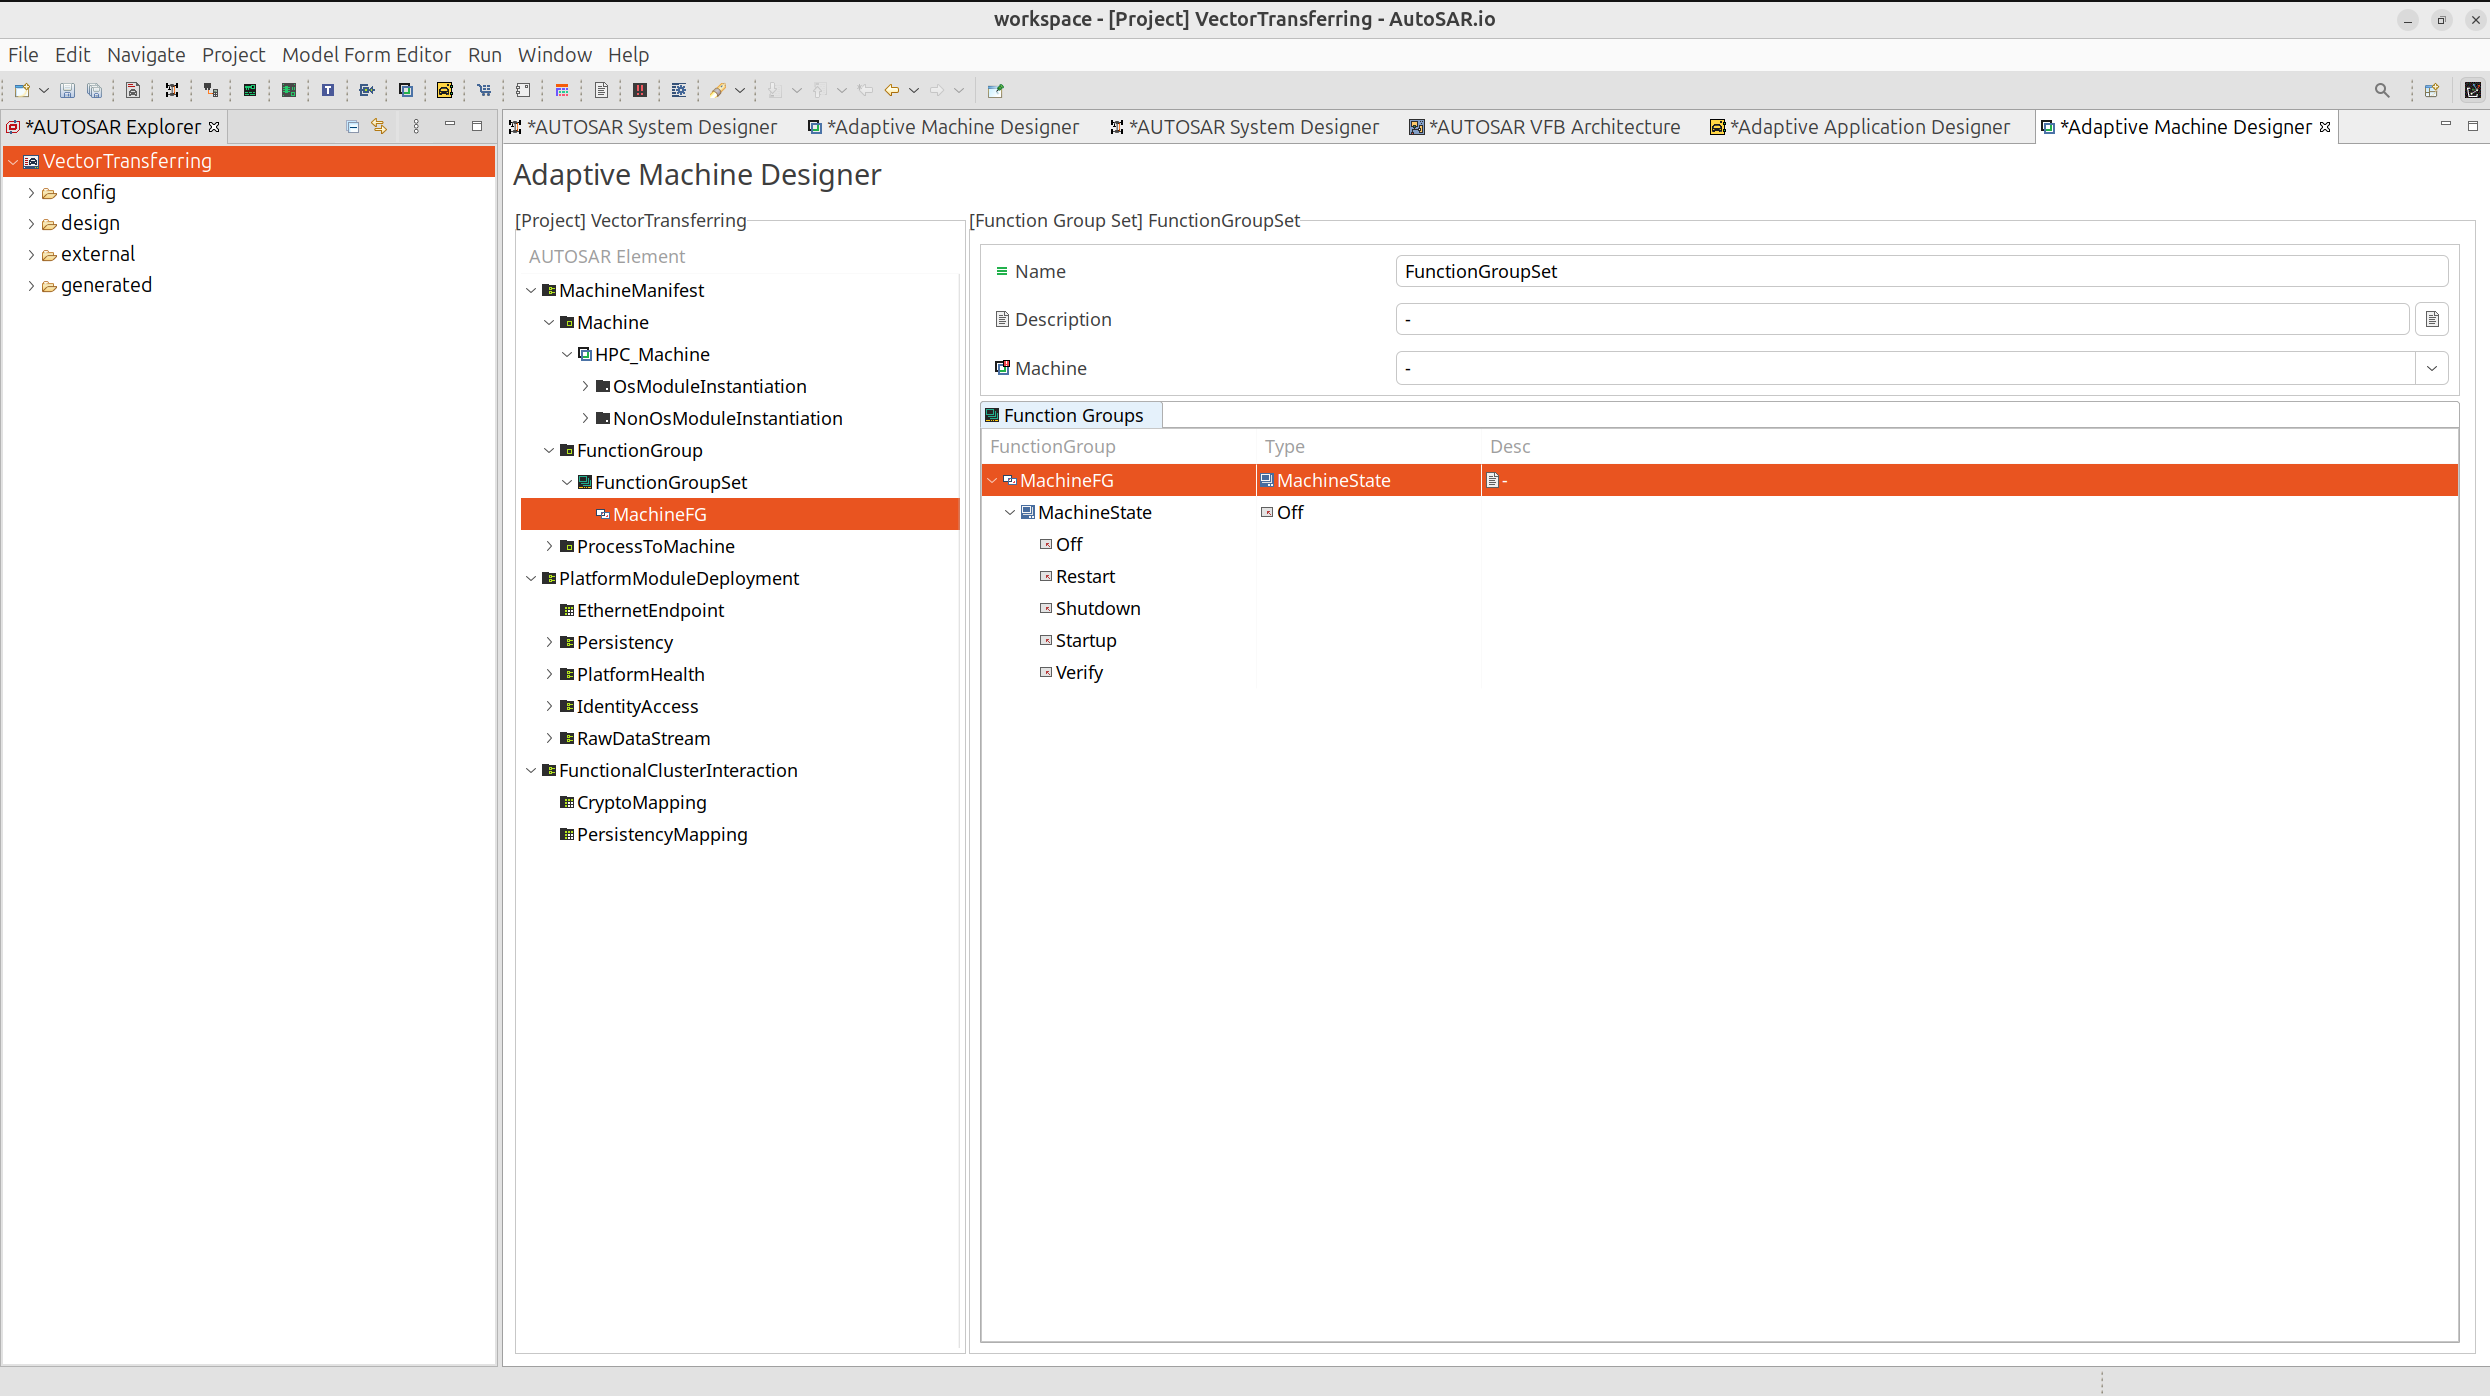
\includegraphics[width=0.75\textwidth]{Images/chap3/image_methodology/machineDesign/configMachineFG.png}
    \vspace{0.5cm}
    \caption{Machine Function Group States Configuration}
    \label{fig:machine_fg_config}
\end{figure}

The figure \ref{fig:machine_fg_config} presents the configuration of the machine function group for the HPC\_Machine in the Adaptive Machine Designer. A function group named MachineFG is defined with the MachineState type, which includes states such as Off, Startup, Verify, Restart, and Shutdown. This configuration governs how the machine progresses through its operational lifecycle, ensuring that platform services and applications are activated and controlled according to well defined system states during runtime execution.

% Final Machine Manifest
\begin{figure}[H]
    \centering
    
\includegraphics[width=0.75\textwidth]{Images/chap3/image_methodology/machineDesign/machineManifest.png}
    \vspace{0.5cm}
    \caption{Machine Manifest for Adaptive AUTOSAR Deployment}
    \label{fig:machine_manifest}
\end{figure}

The figure \ref{fig:machine_manifest} presents the Machine Manifest of the HPC\_Machine as defined in the Adaptive Machine Designer. This manifest consolidates all machine level configurations by referencing the previously defined Machine Design, including the SOME/IP Service Discovery endpoint with the multicast address 224.0.0.1 and port 30490, as well as the Ethernet connector bound to the eth0 interface. In addition, user defined connectors and inter process communication settings are integrated, forming a complete description of the communication capabilities of the target machine.

Furthermore, the manifest specifies essential execution and platform related properties such as trusted platform execution mode, default application timeout, and processor configuration. The processor section defines the available CPU resources and core assignment, while function group and process to machine mappings establish how applications are bound to machine states at runtime. By combining communication, execution, and lifecycle information into a single artifact, the Machine Manifest serves as the final deployment blueprint for Adaptive AUTOSAR applications.

% Configure Operating System platform module
\begin{figure}[H]
    \centering
    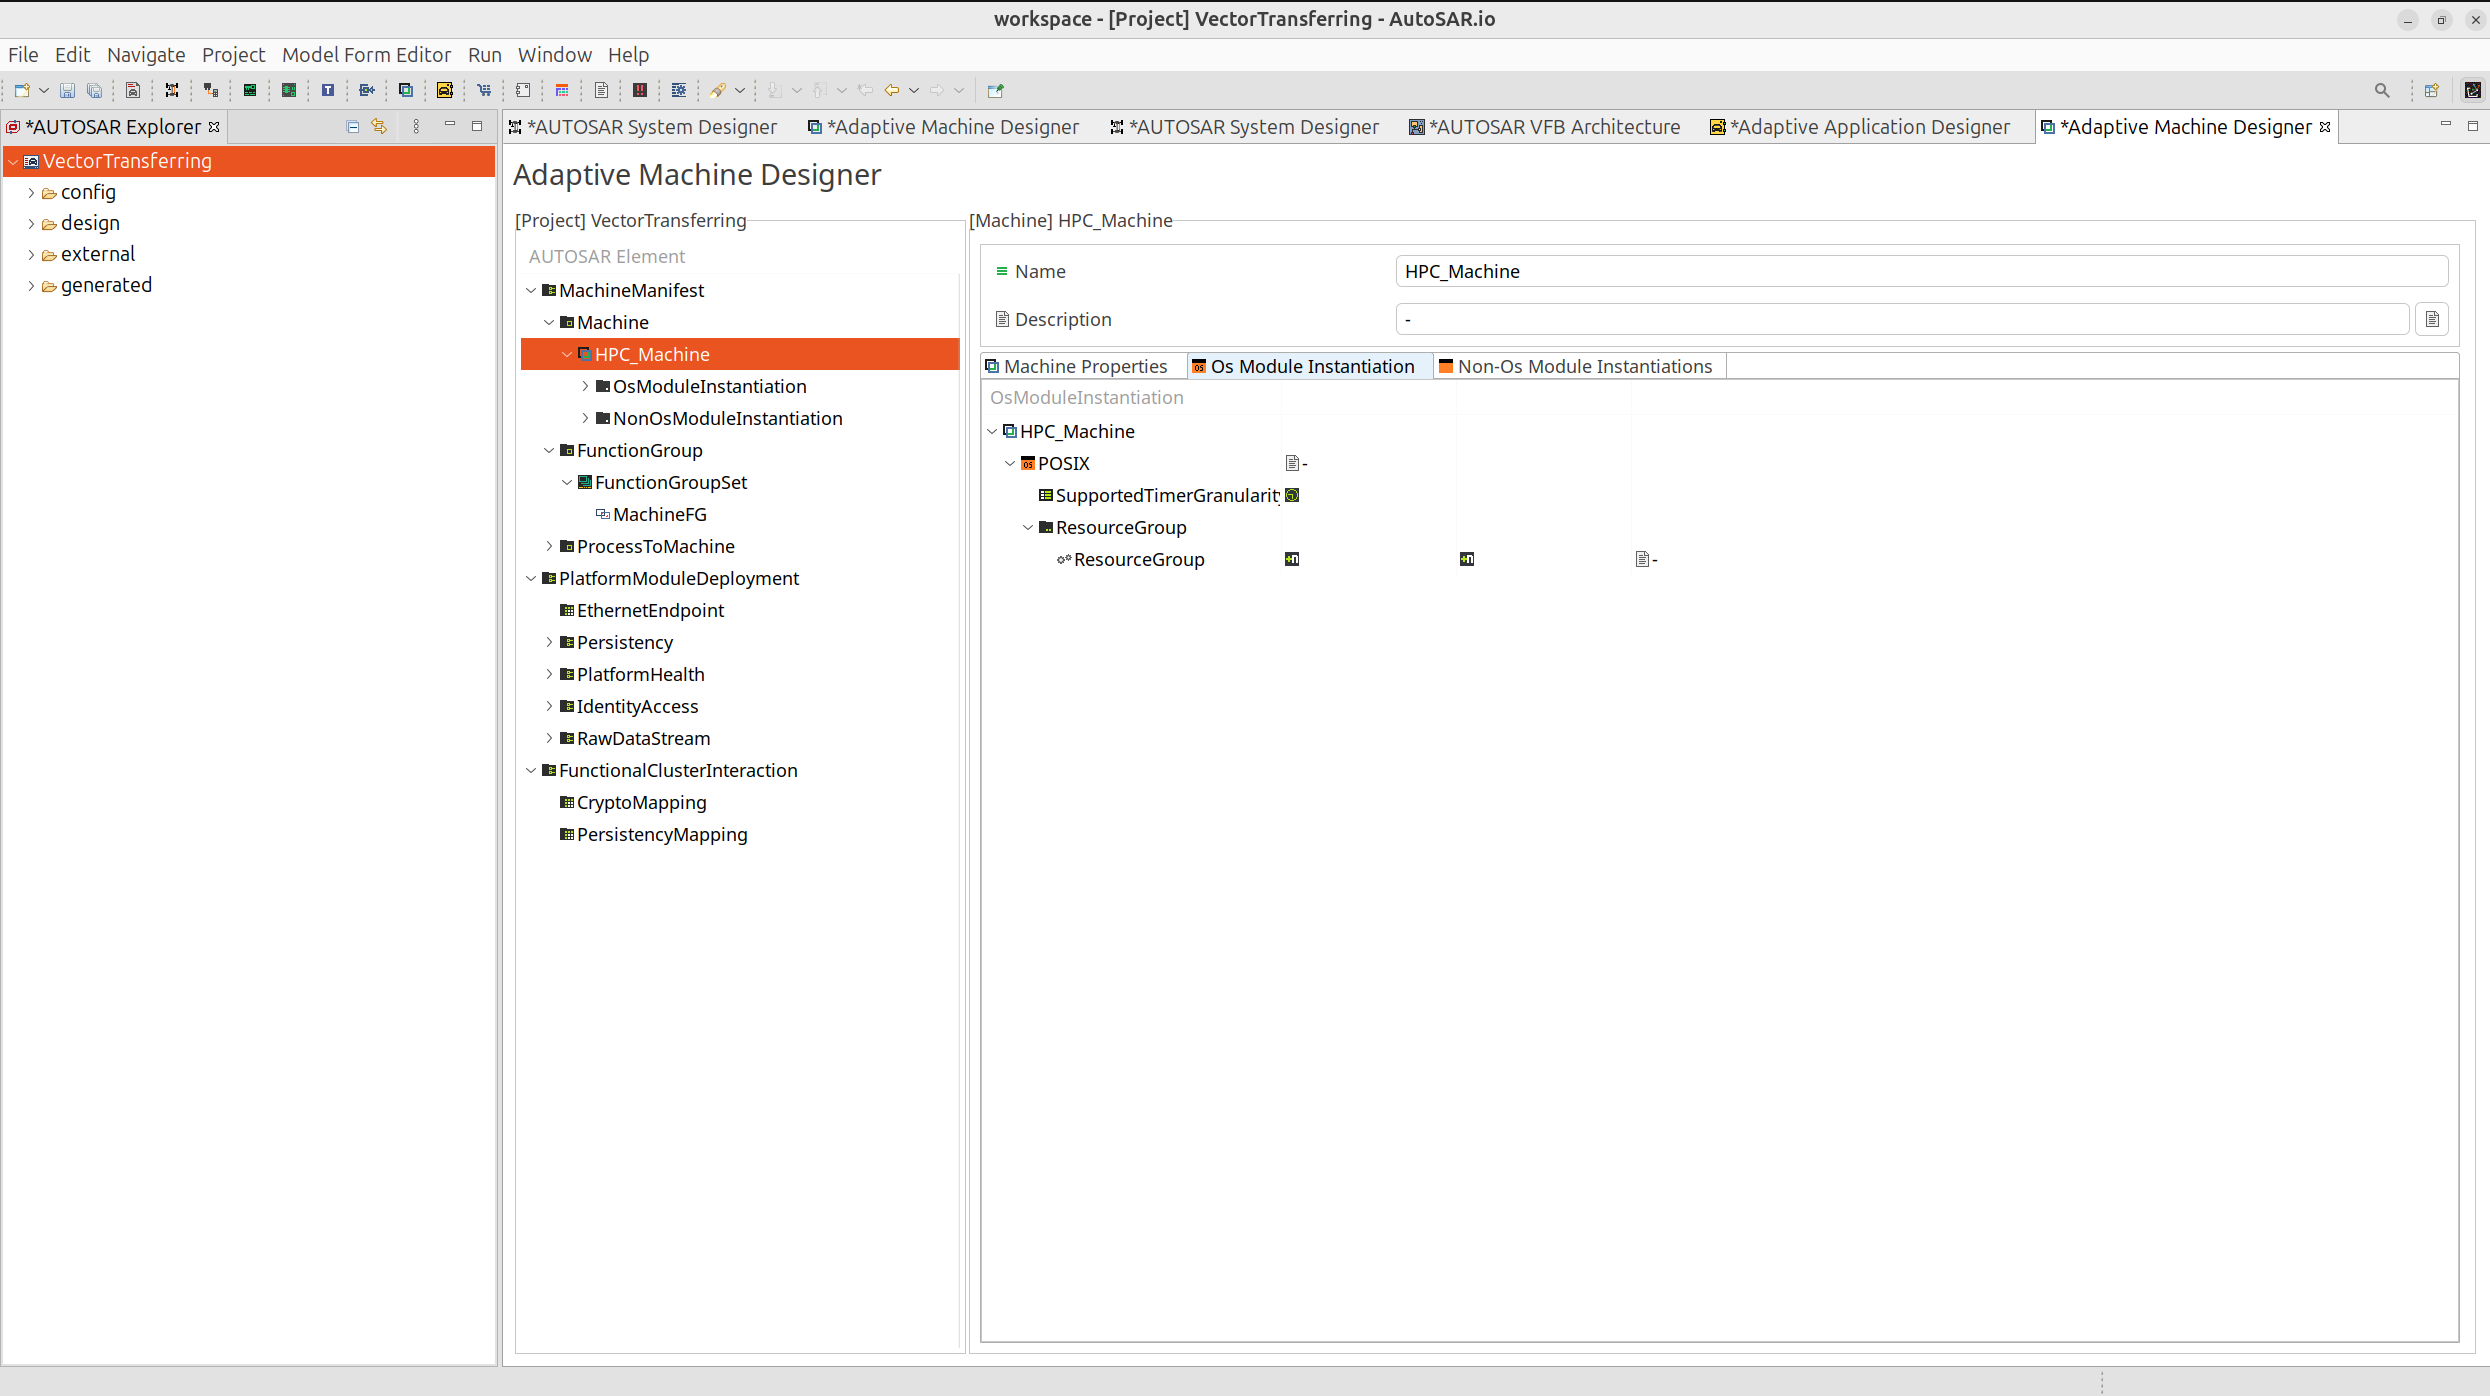
\includegraphics[width=0.75\textwidth]{Images/chap3/image_methodology/machineDesign/configOSModule.png}
    \vspace{0.5cm}
    \caption{Operating System Platform Module Configuration}
    \label{fig:machine_os_module}
\end{figure}

Figure~\ref{fig:machine_os_module} shows the operating system platform module configuration for the target machine named HPC\_Machine in the Adaptive Machine Designer. The POSIX based operating system module is instantiated to define the execution environment for Adaptive AUTOSAR applications, including supported timer granularity and resource group settings. This configuration establishes the fundamental runtime services required for process scheduling and resource management on the target machine.

% Configure non-OS platform modules
\begin{figure}[H]
    \centering
    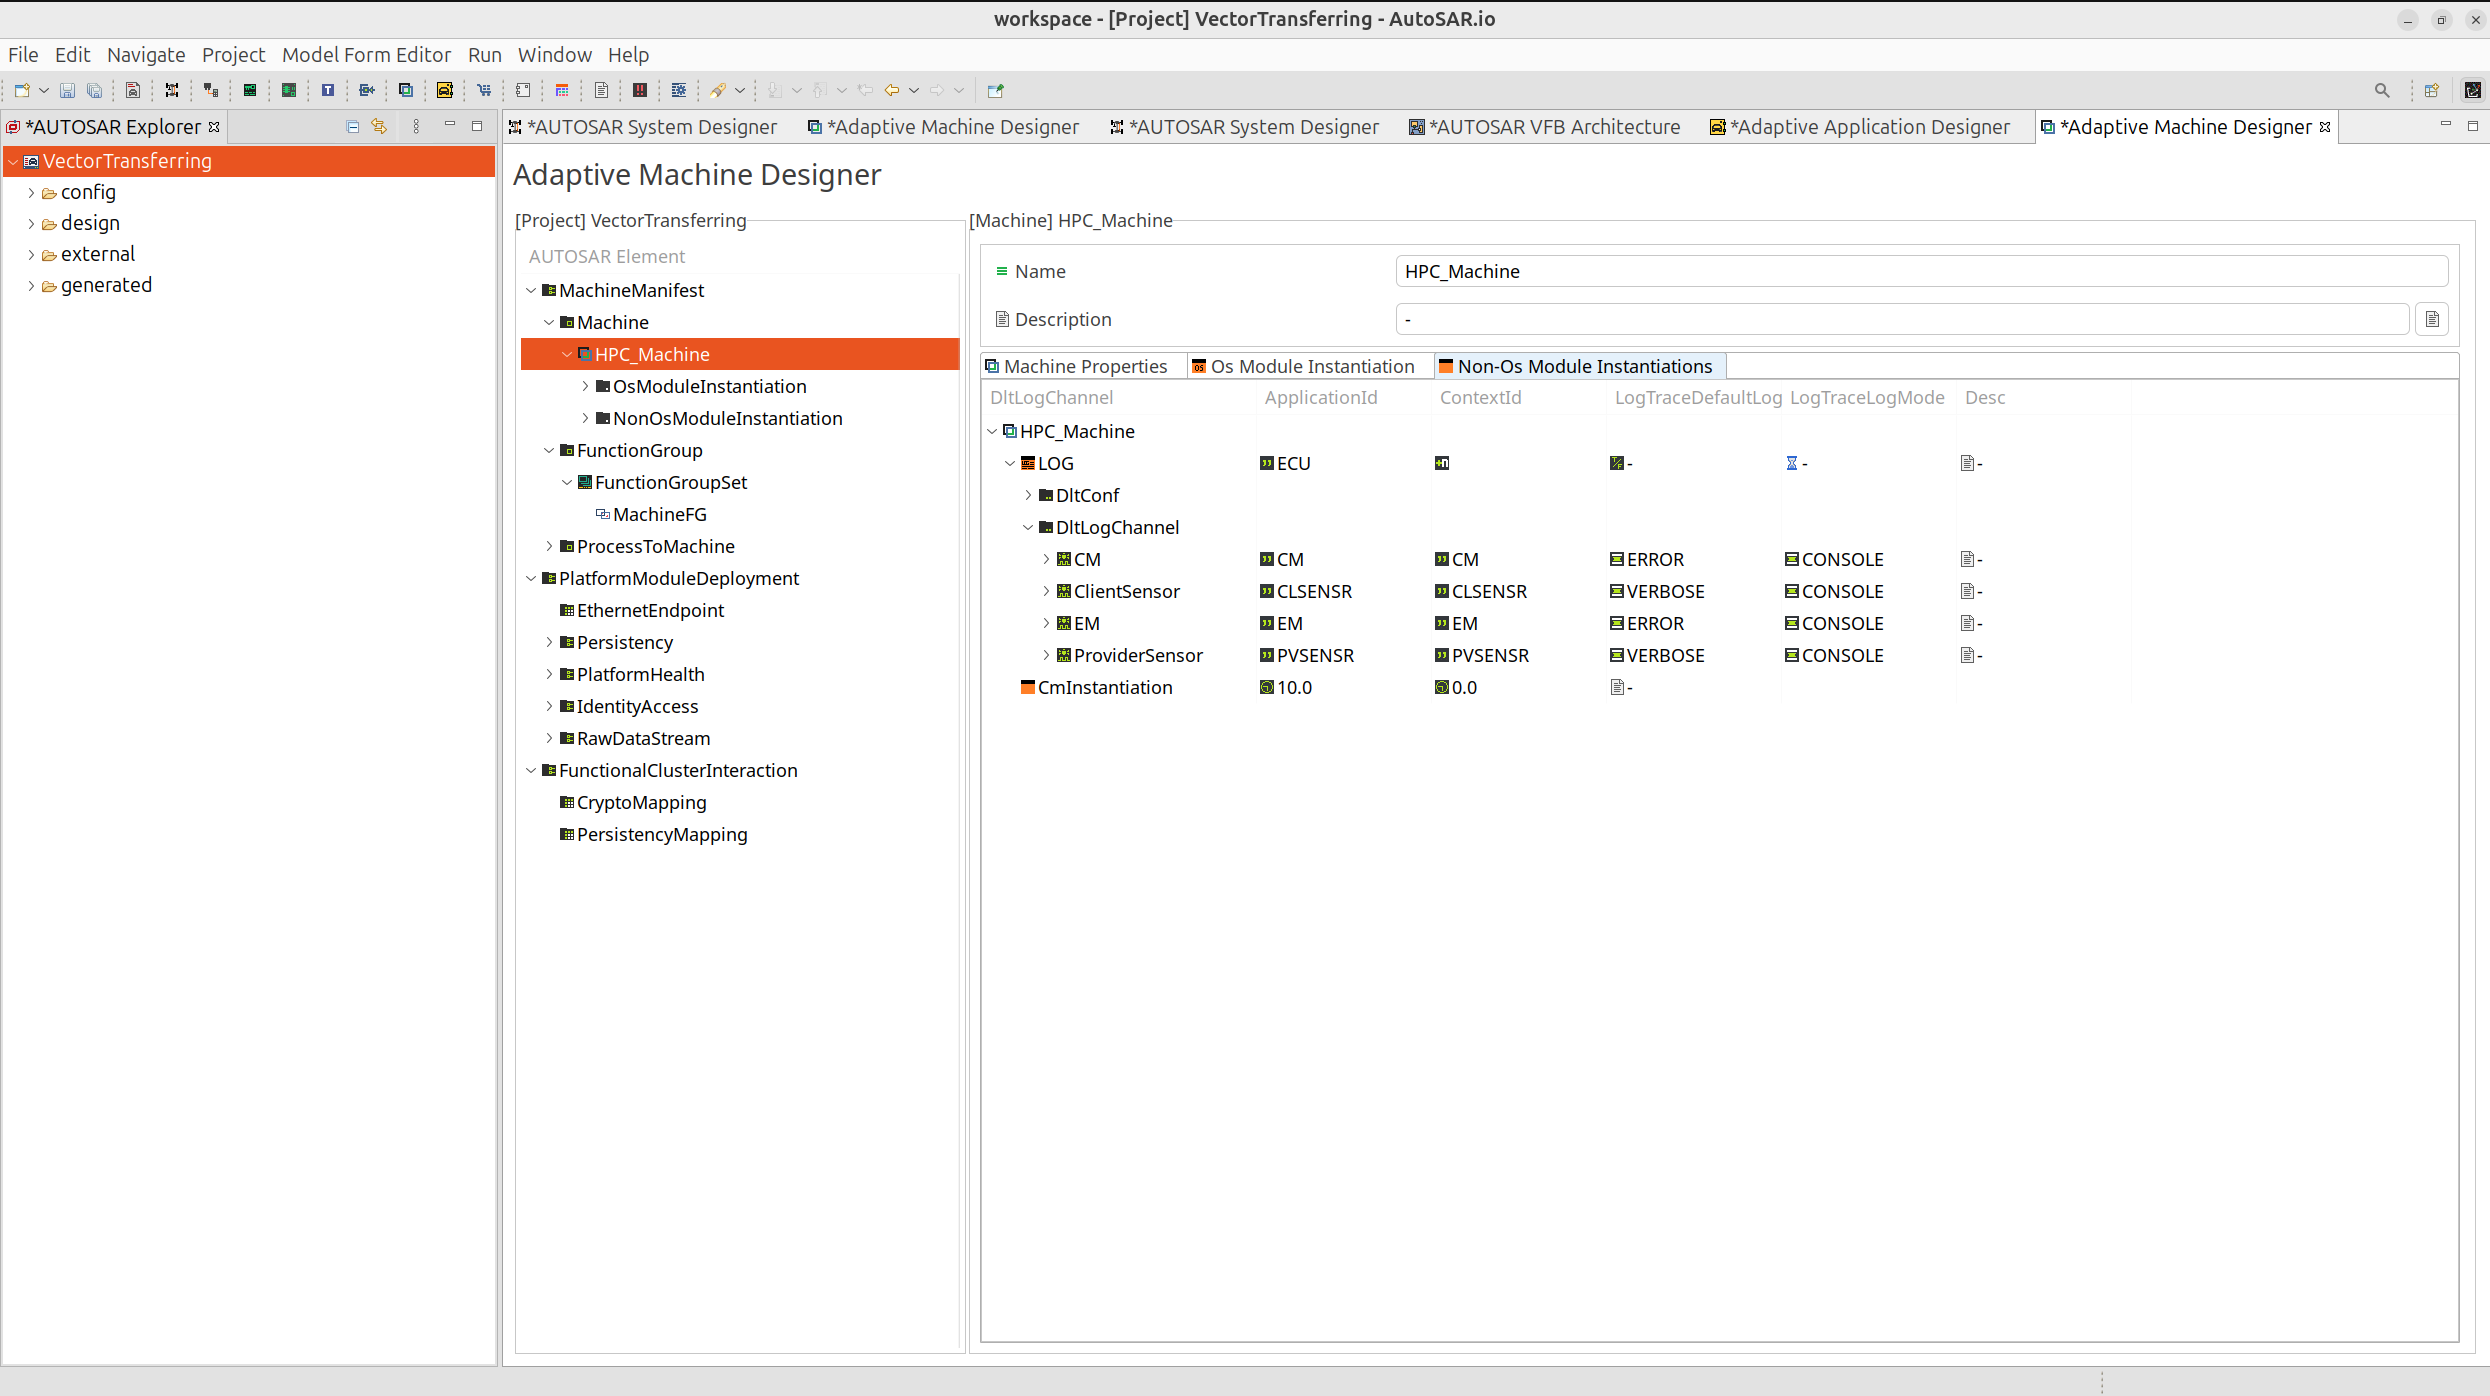
\includegraphics[width=0.75\textwidth]{Images/chap3/image_methodology/machineDesign/configNonOS.png}
    \vspace{0.5cm}
    \caption{Configuration of Non-OS Platform Modules}
    \label{fig:machine_non_os_module}
\end{figure}

Figure~\ref{fig:machine_non_os_module} presents the configuration of Diagnostic Log and Trace for the HPC\_Machine in the Adaptive Machine Designer. Several log channels are defined for different software entities, including ECU, ClientSensor, EM, and ProviderSensor, each mapped to a distinct ApplicationId and ContextId. Log levels such as ERROR and VERBOSE are specified, and the output is directed to the console, allowing developers to monitor application execution and diagnose runtime behavior.

In addition, the configuration highlights the role of CMInstantiation, which represents the Communication Management daemon responsible for inter process communication on the Adaptive Platform. This daemon enables different processes to exchange messages and supports the transport of diagnostic data between applications and platform services. By instantiating the communication manager at the machine level, the system ensures that logging, tracing, and service communication operate coherently across all running processes.

\subsubsection{Service Interface Design and Mapping}

% Define data types for service interfaces
\begin{figure}[H]
    \centering
    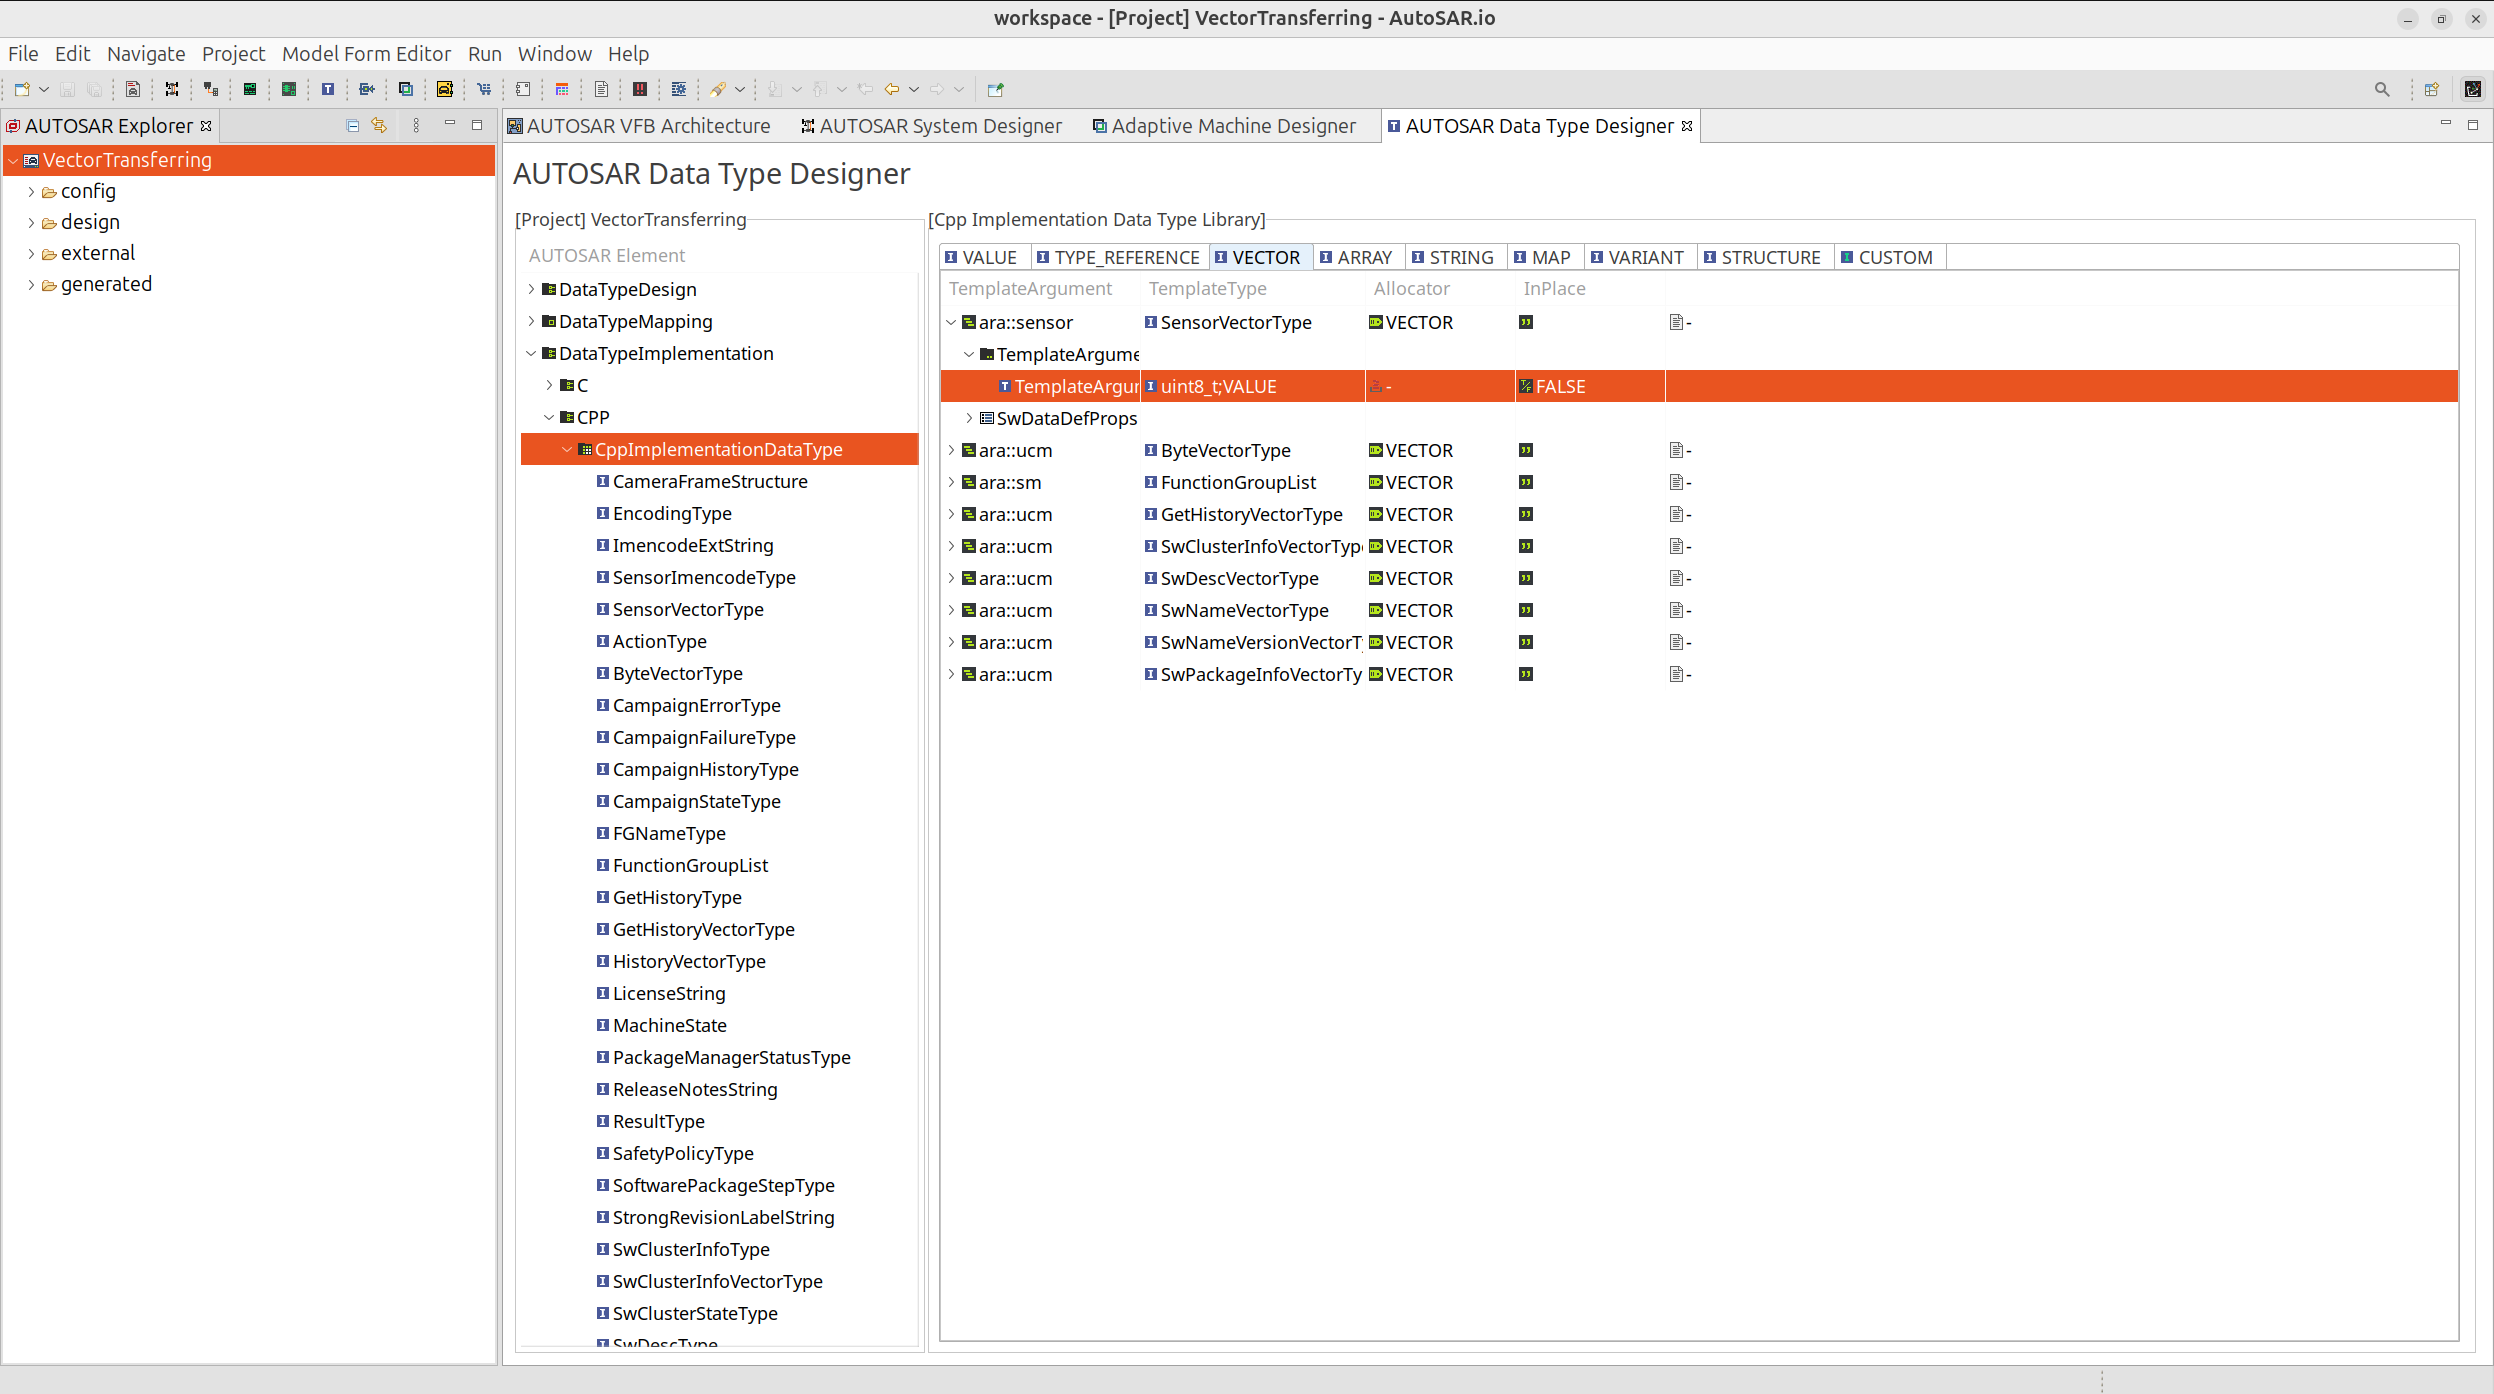
\includegraphics[width=0.75\textwidth]{Images/chap3/image_methodology/serviceInterfaceDesign/dataType.png}
    \vspace{0.5cm}
    \caption{Definition of Data Types for Service Interfaces}
    \label{fig:service_datatype}
\end{figure}

The figure~\ref{fig:service_datatype} shows the specification of C++ data types used to support service interfaces in the Adaptive AUTOSAR environment. Several vector based types are defined using template arguments, where primitive elements such as \texttt{uint8\_t} are combined to represent structured service data. These type definitions provide a clear and reusable foundation for data exchange between service providers and consumers, ensuring consistency and type safety during service oriented communication.

% Define service interface
\begin{figure}[H]
    \centering
    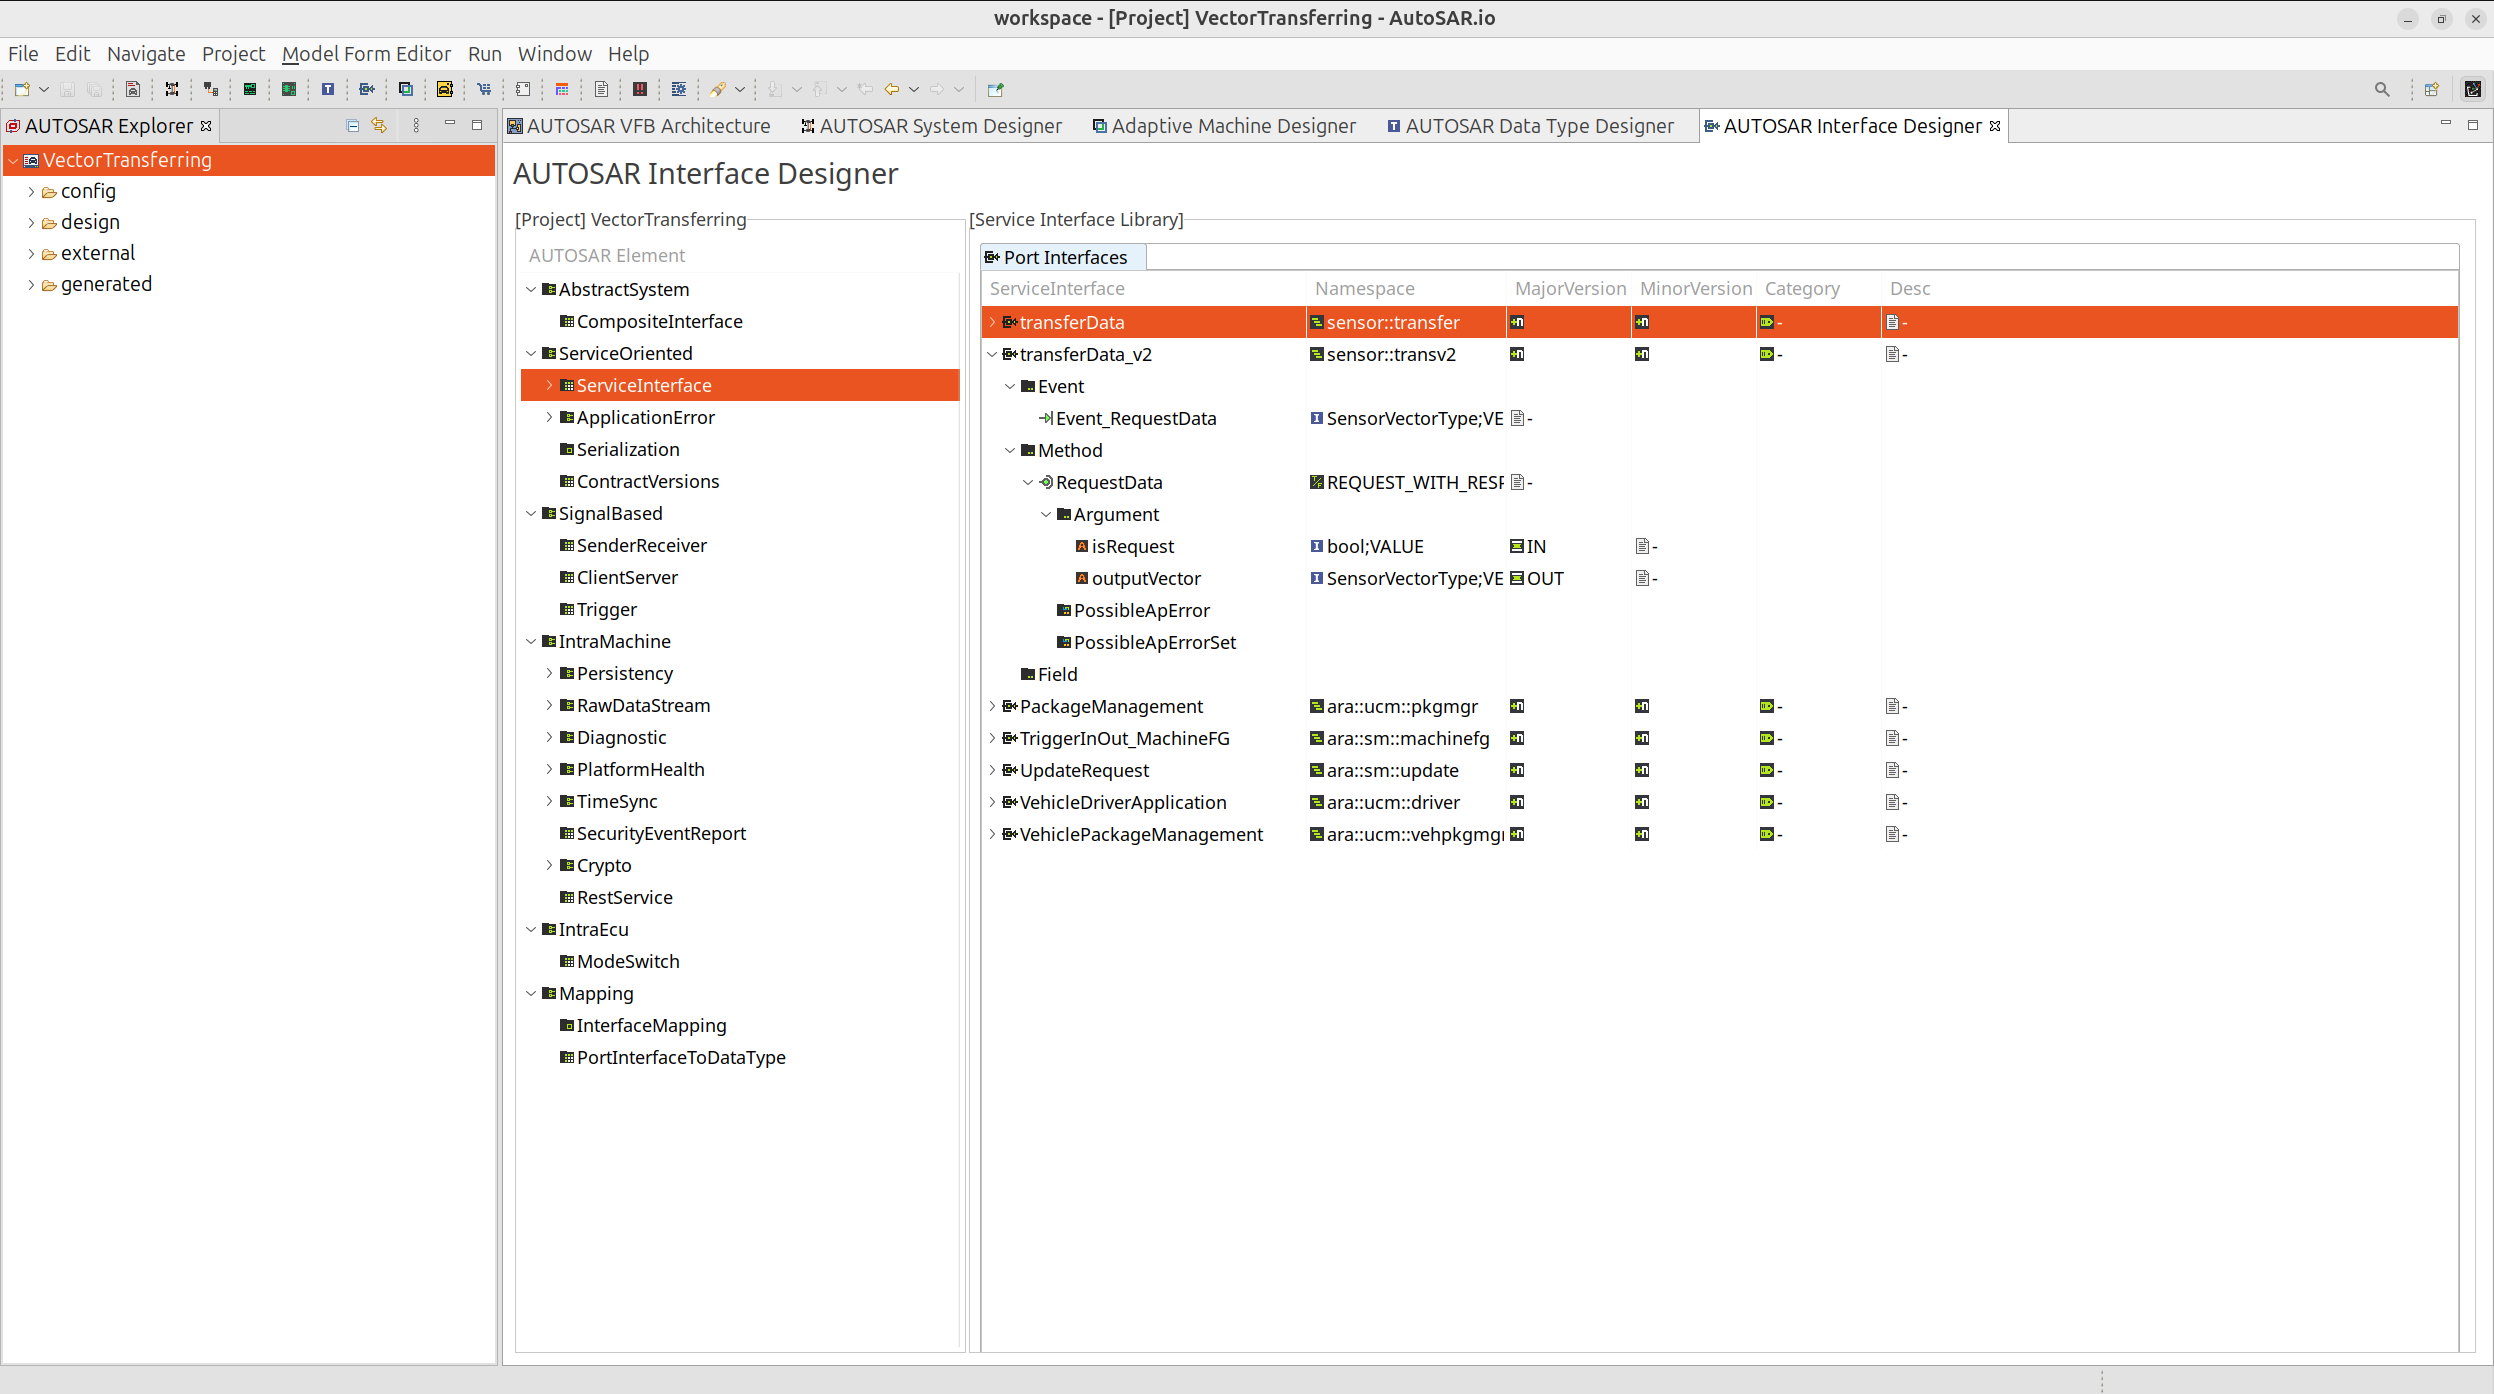
\includegraphics[width=0.75\textwidth]{Images/chap3/image_methodology/serviceInterfaceDesign/defineServiceInterface.png}
    \vspace{0.5cm}
    \caption{Service Interface Definition in Adaptive AUTOSAR}
    \label{fig:service_interface_definition}
\end{figure}

Figure~\ref{fig:service_interface_definition} illustrates the definition of a service oriented interface in the AUTOSAR Interface Designer. The service interface named \texttt{transferData\_v2} is specified within the \texttt{sensor::transv2} namespace and versioned to support interface evolution. It exposes both an event and a method, where the event enables asynchronous notification of data availability, while the method defines a request response interaction pattern for controlled data transmission between applications.

In addition, the interface description includes detailed method arguments and data flow directions. The \texttt{RequestData} method accepts an input parameter that influences the request behavior and produces an output vector based on the previously defined sensor data type. The event is associated with the same data representation (\texttt{Event\_RequestData}), allowing consumers to receive updates without explicitly issuing a request. Possible application errors are also declared to handle exceptional conditions during execution. As shown in Figure~\ref{fig:service_interface_definition}, this interface design supports both reactive and on demand communication between service providers and consumers in the Adaptive AUTOSAR system.


% Service deployment configuration
\begin{figure}[H]
    \centering
    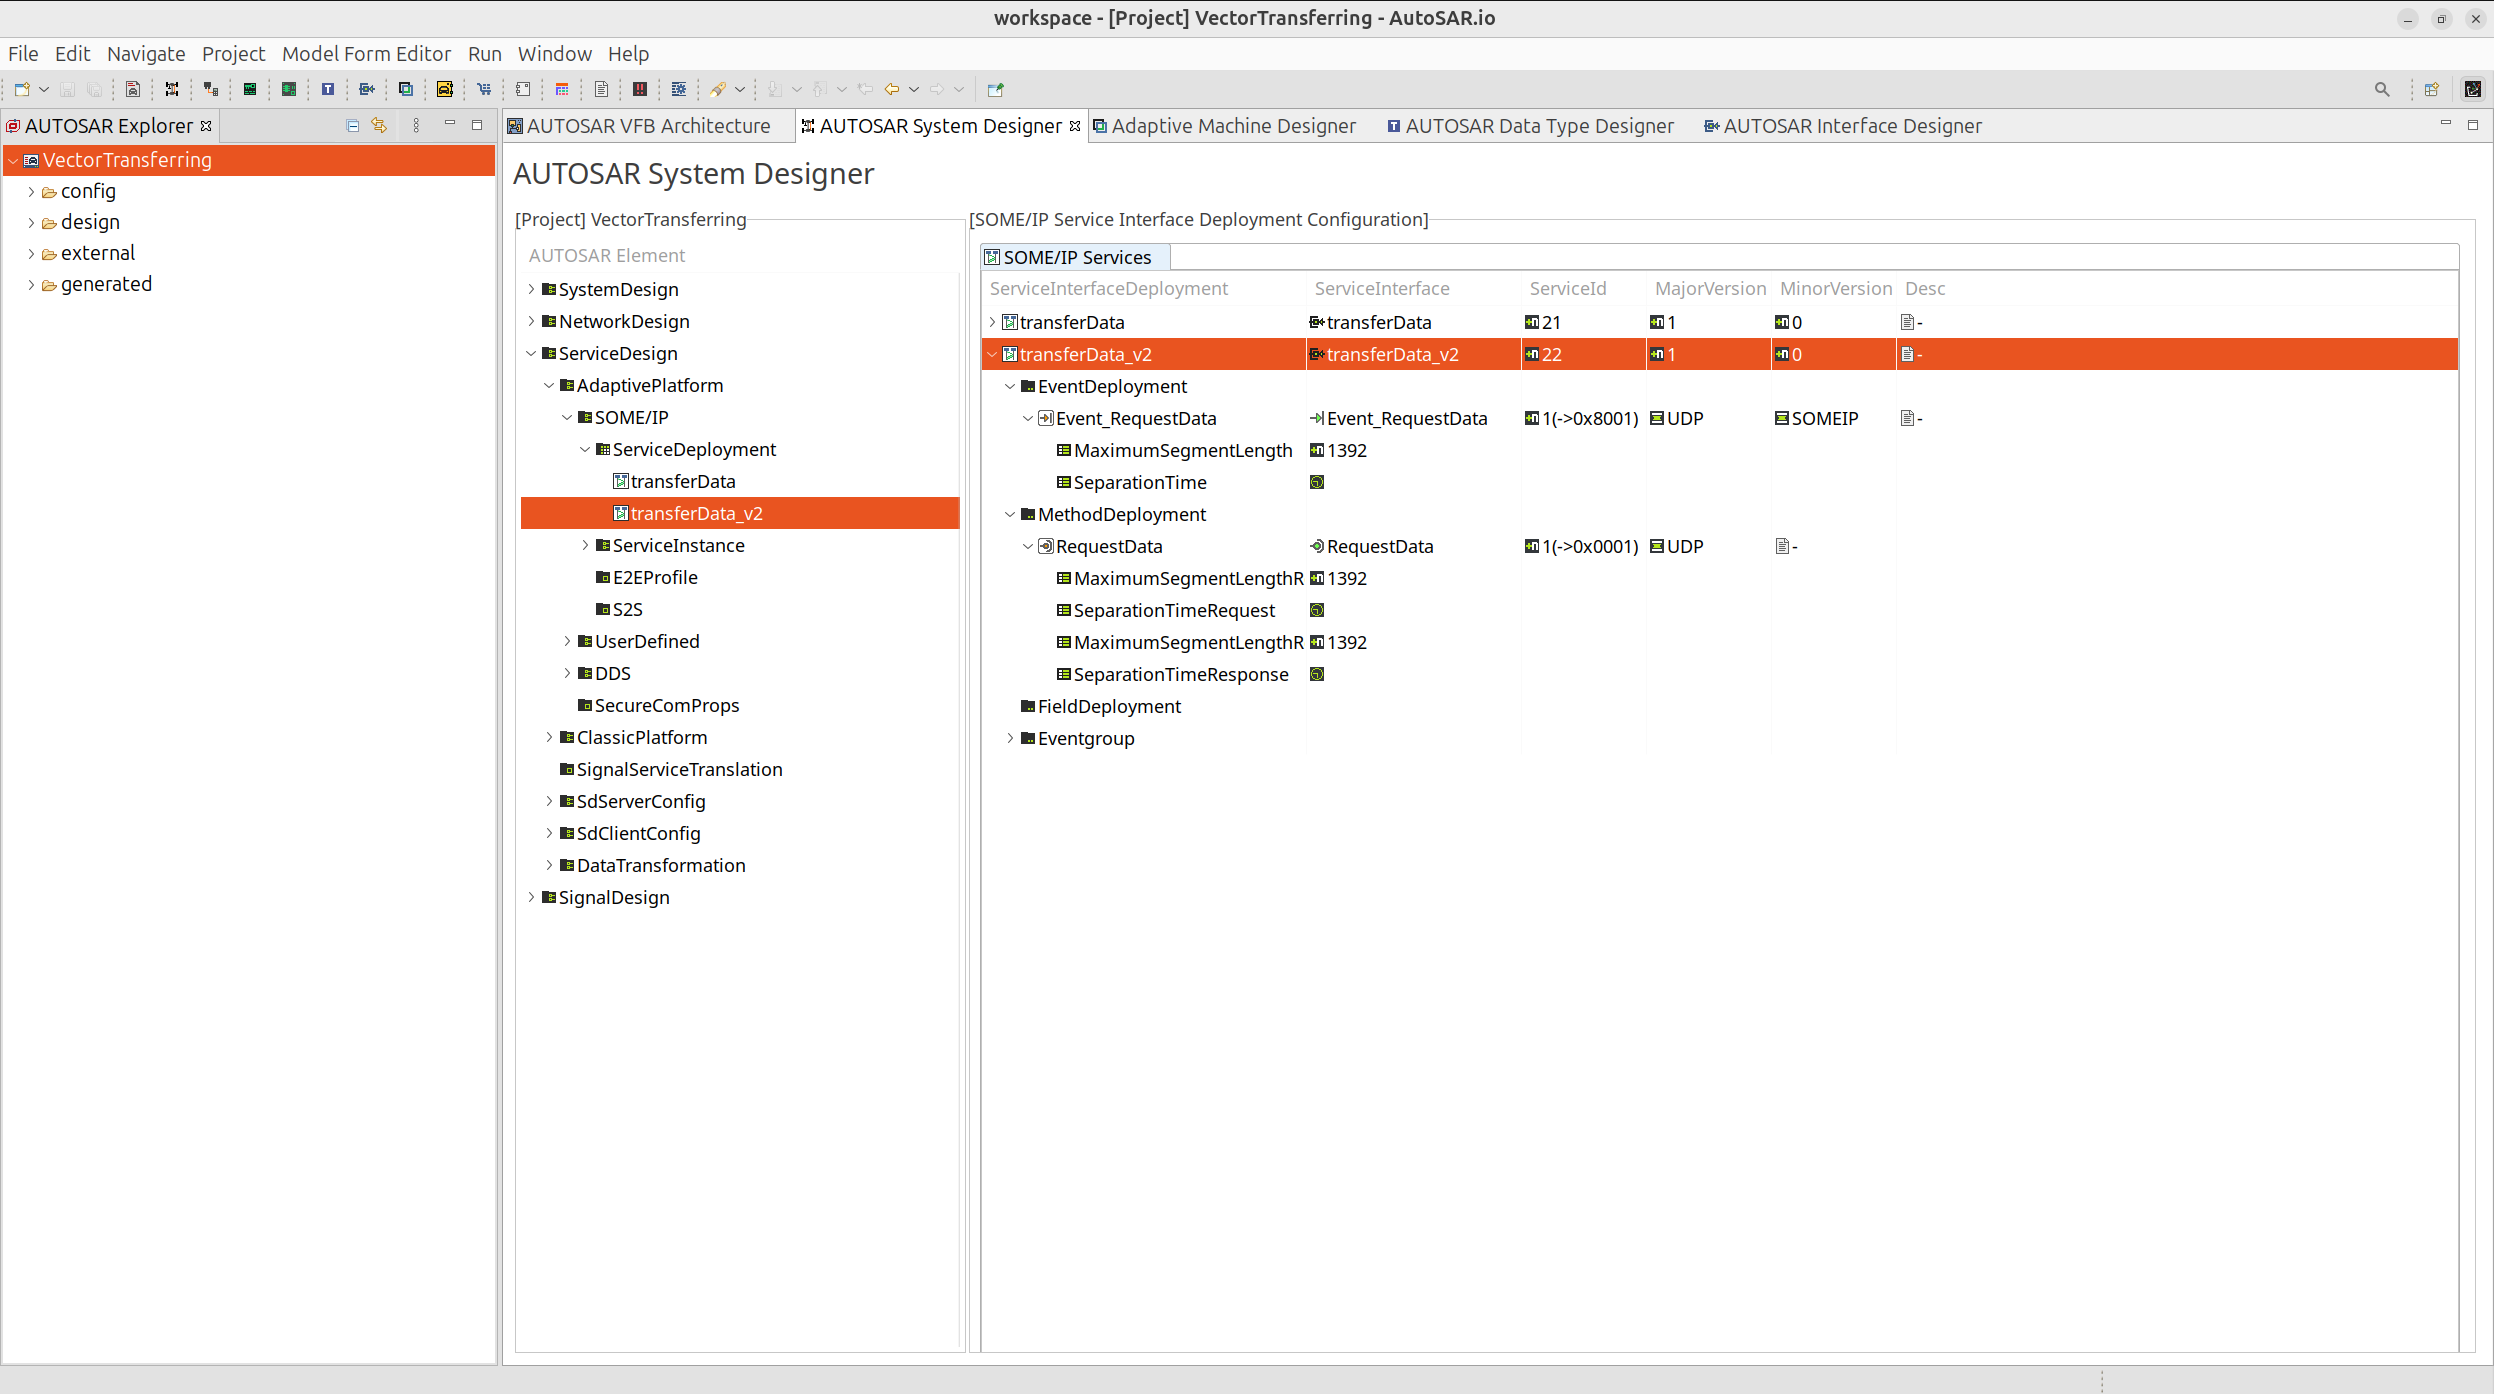
\includegraphics[width=0.75\textwidth]{Images/chap3/image_methodology/serviceInterfaceDesign/serviceDeployment.png}
    \vspace{0.5cm}
    \caption{Service Deployment Configuration}
    \label{fig:service_deployment}
\end{figure}

Figure~\ref{fig:service_deployment} illustrates the SOME/IP service deployment configuration for the \texttt{transferData\_v2} interface within the AUTOSAR System Designer. In this project, the service is explicitly deployed over SOME/IP with transport protocol (SOME/IP-TP) to support the transmission of large data payloads, such as image frames, between the ProviderSensor and ClientSensor applications.

The service is assigned a unique service identifier and version number and includes both event-based and method-based communication. The event \texttt{Event\_RequestData} is configured to use UDP transport together with a specified \texttt{MaximumSegmentLength}. This parameter plays a critical role in enabling SOME/IP-TP, as it informs the Adaptive AUTOSAR middleware that the transmitted data may exceed the maximum payload size of a single UDP packet and therefore must be segmented and reassembled at the receiver side.

Without configuring the \texttt{MaximumSegmentLength}, the communication would default to standard SOME/IP over UDP, which is suitable only for small messages and is not appropriate for transmitting image data. By explicitly defining this parameter, the deployment ensures that image payloads generated by the ProviderSensor are correctly fragmented, transmitted, and reassembled by the ClientSensor.

In addition to the event deployment, the \texttt{RequestData} method deployment specifies request and response timing parameters, supporting controlled client–server interaction when on-demand data transfer is required. Together, these configurations ensure that the \texttt{transferData\_v2} service can be reliably discovered via Service Discovery and can support both event-driven and request-based communication over SOME/IP-TP during runtime execution.


% Service instance provider configuration
\begin{figure}[H]
    \centering
    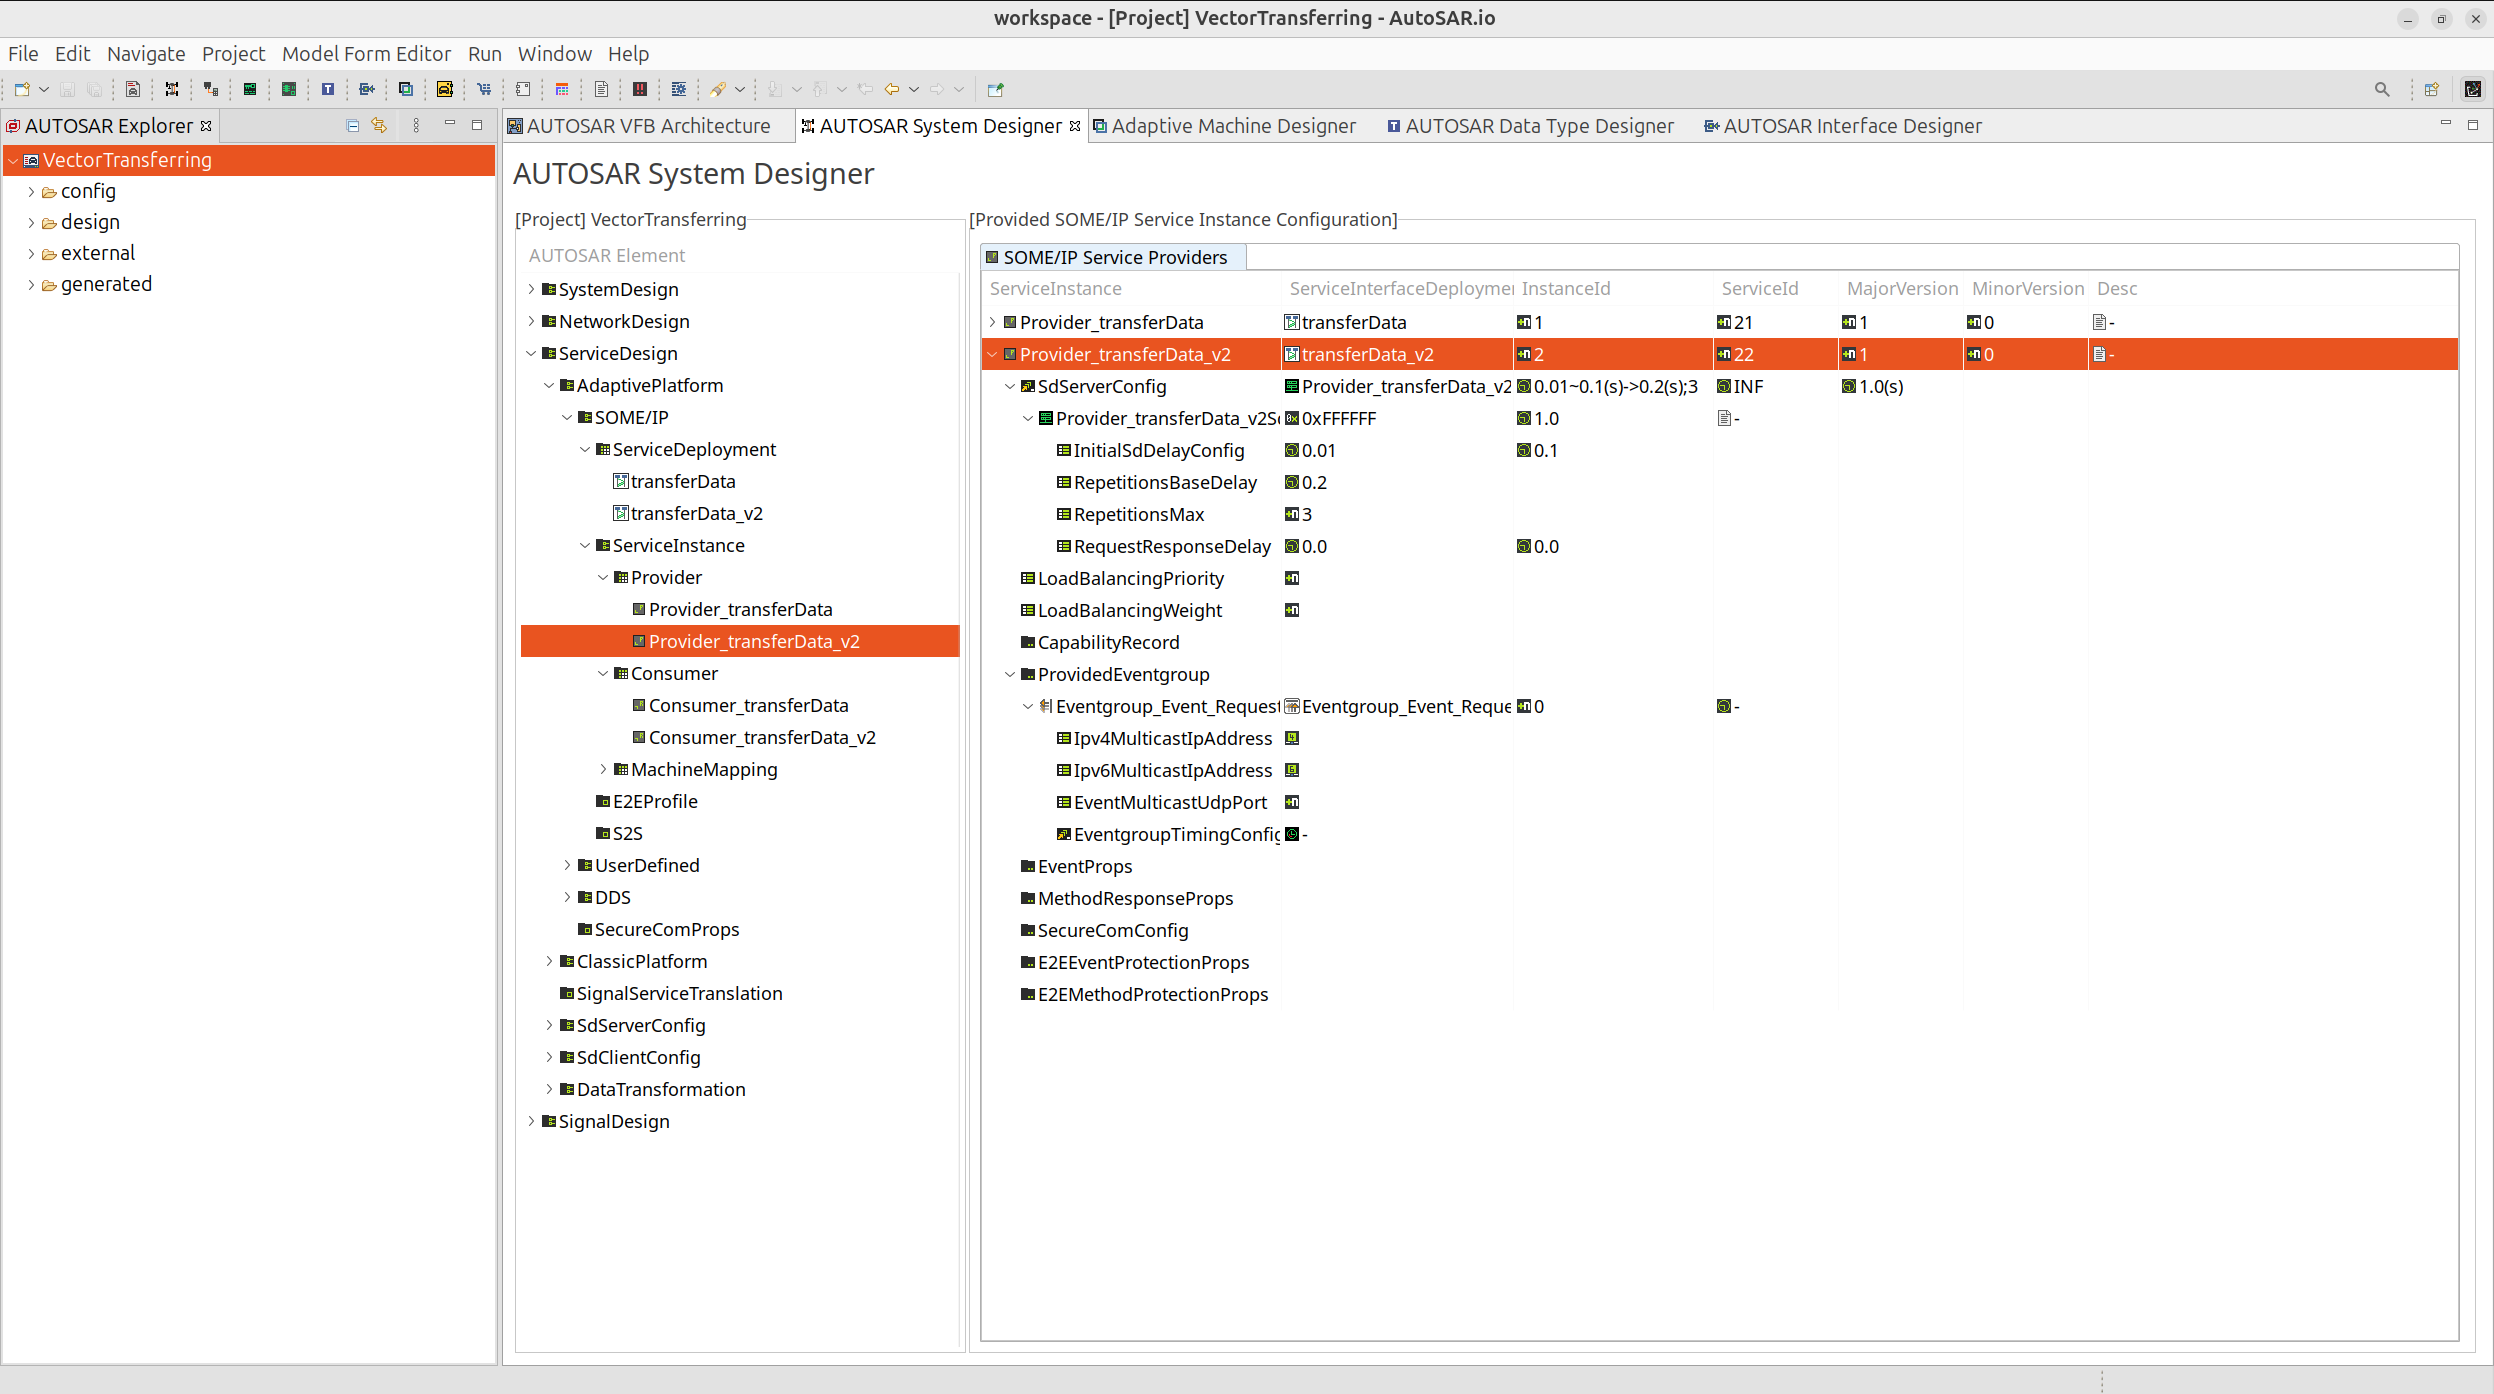
\includegraphics[width=0.75\textwidth]{Images/chap3/image_methodology/serviceInterfaceDesign/serviceInstance_Provider.png}
    \vspace{0.5cm}
    \caption{Service Instance Configuration for Provider}
    \label{fig:service_instance_provider}
\end{figure}

Figure~\ref{fig:service_instance_provider} illustrates the configuration of the SOME/IP service provider for the \texttt{transferData\_v2} interface. The provider instance is bound to a specific service and instance identifier with a defined major and minor version, ensuring compatibility with consuming applications. Server side parameters such as initial service offer delay, repetition base delay, and maximum repetitions are configured to control service availability announcements via Service Discovery. In addition, the provider defines event group settings for data notifications, together with timing and response related properties, which enable reliable dissemination of event based data to subscribed consumers during runtime.

% Service instance consumer configuration
\begin{figure}[H]
    \centering
    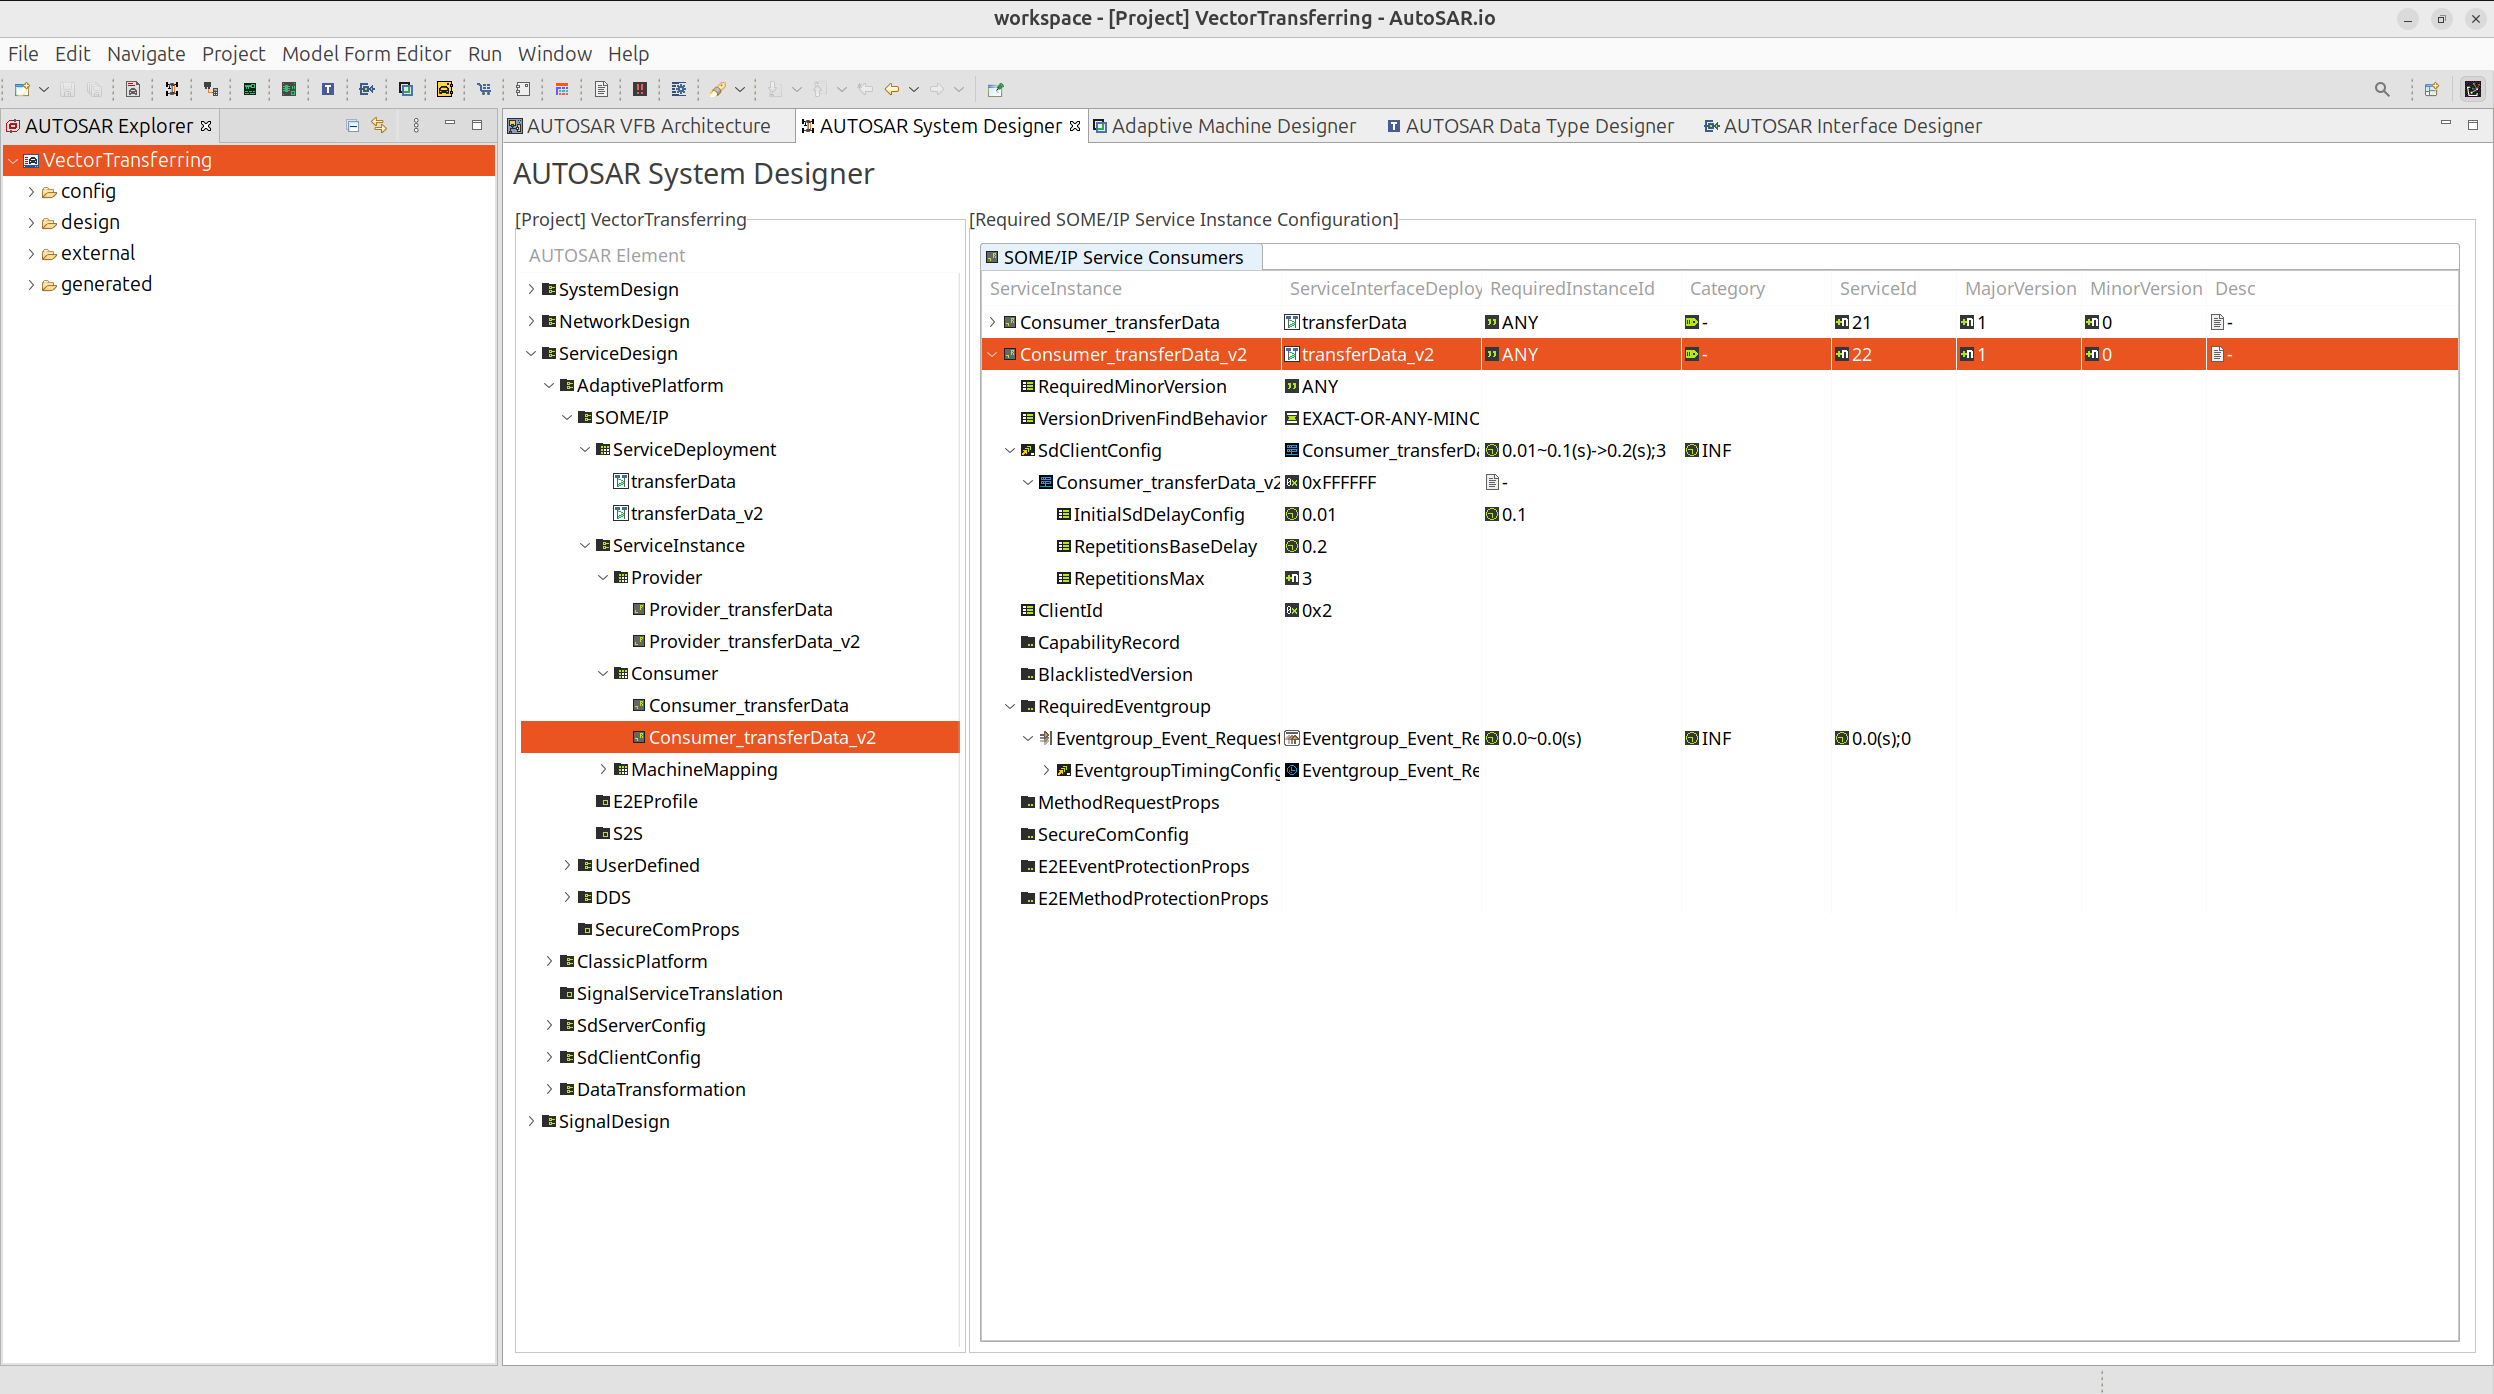
\includegraphics[width=0.75\textwidth]{Images/chap3/image_methodology/serviceInterfaceDesign/serviceInstance_Consumer.png}
    \vspace{0.5cm}
    \caption{Service Instance Configuration for Consumer}
    \label{fig:service_instance_consumer}
\end{figure}

Figure~\ref{fig:service_instance_consumer} presents the configuration of the corresponding SOME/IP service consumer acting as a subscriber to the \texttt{transferData\_v2} service. The consumer specifies flexible version requirements and discovery behavior, allowing it to bind to compatible provider instances at runtime. Client side parameters such as initial request delay, repetition strategy, and event group subscription settings determine how the consumer discovers the service and receives event notifications. Through this configuration, the consumer can dynamically subscribe to published data while maintaining controlled request and subscription behavior within the Adaptive AUTOSAR communication framework.

% Mapping service to machine network endpoint
\begin{figure}[H]
    \centering
    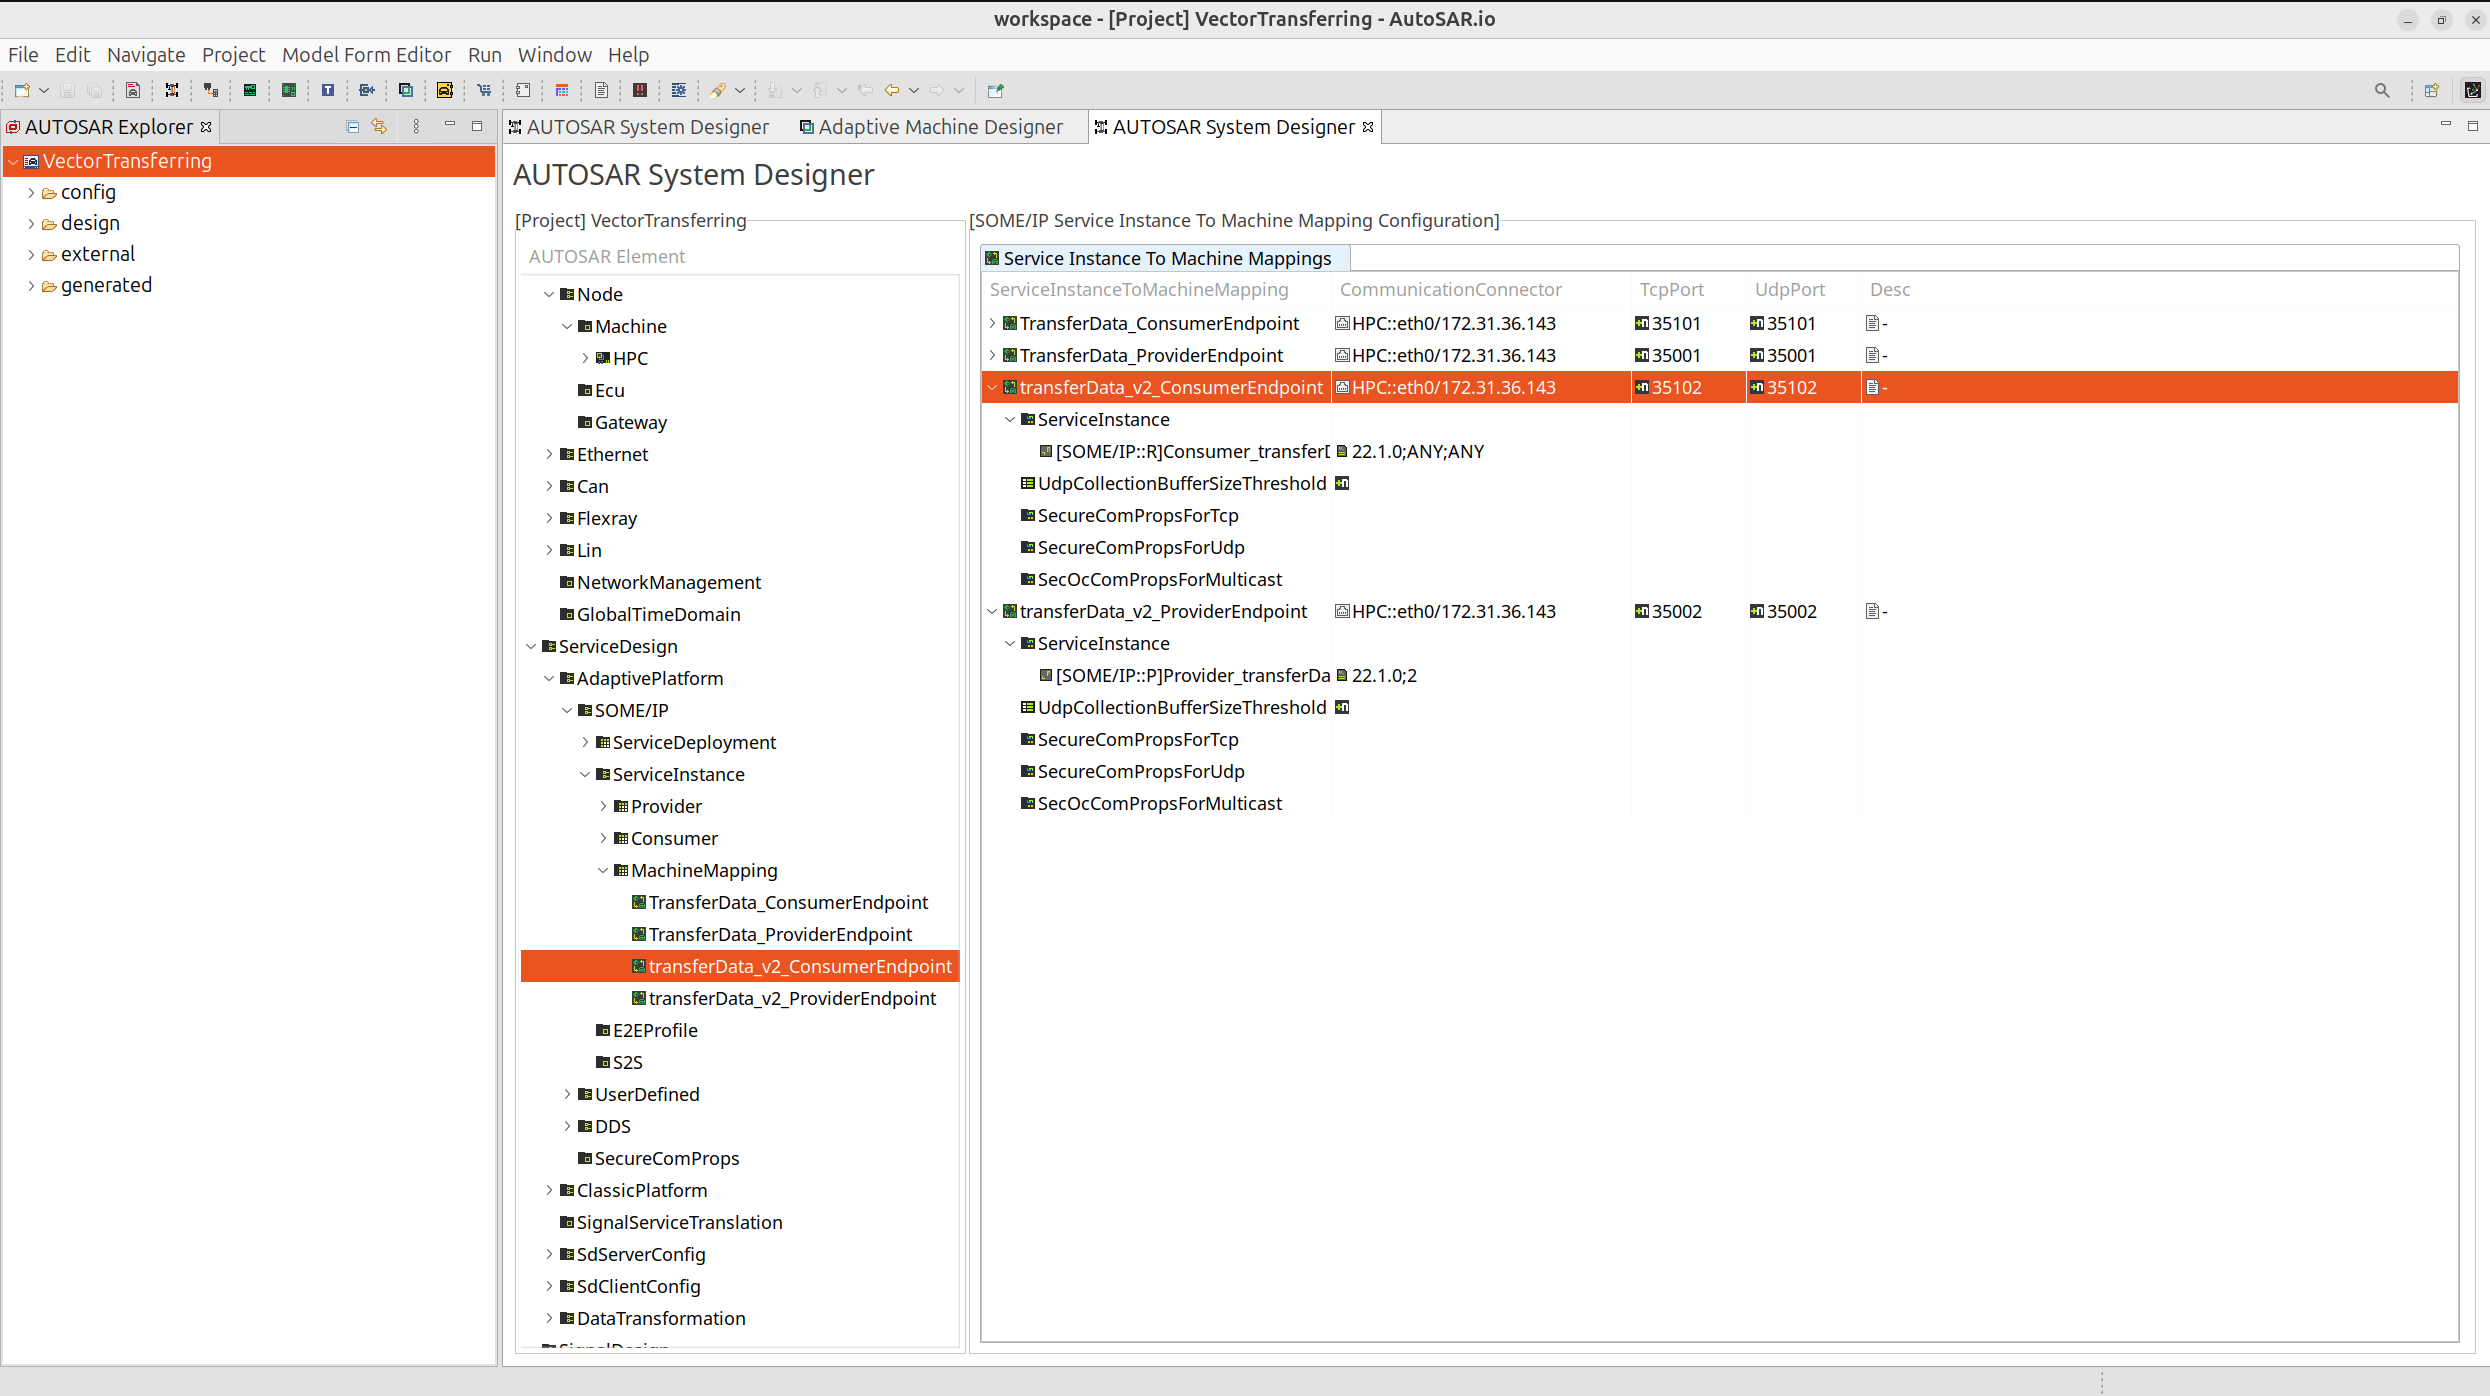
\includegraphics[width=0.75\textwidth]{Images/chap3/image_methodology/serviceInterfaceDesign/serviceMappingMachineEndpoint.png}
    \vspace{0.5cm}
    \caption{Mapping Service Instances to Machine Network Endpoint}
    \label{fig:service_machine_endpoint_mapping}
\end{figure}

Figure~\ref{fig:service_machine_endpoint_mapping} illustrates how the service instances of the \texttt{transferData} and \texttt{transferData\_v2} interfaces are bound to concrete machine network endpoints. Both provider and consumer instances are mapped to the Ethernet communication connector \texttt{HPC:eth0} with the fixed IPv4 address \texttt{172.31.36.143}, ensuring that all service communication is routed through a well defined network interface. Distinct TCP and UDP port numbers are assigned to each service instance, allowing concurrent data exchange while avoiding port conflicts.

This mapping explicitly links abstract service definitions to physical network resources, enabling correct runtime deployment and communication over SOME/IP. By defining separate endpoints for provider and consumer roles, the configuration supports clear role separation and reliable message routing between applications deployed on the same machine or across different nodes in the Adaptive AUTOSAR system.

\begin{figure}[H]
    \centering
    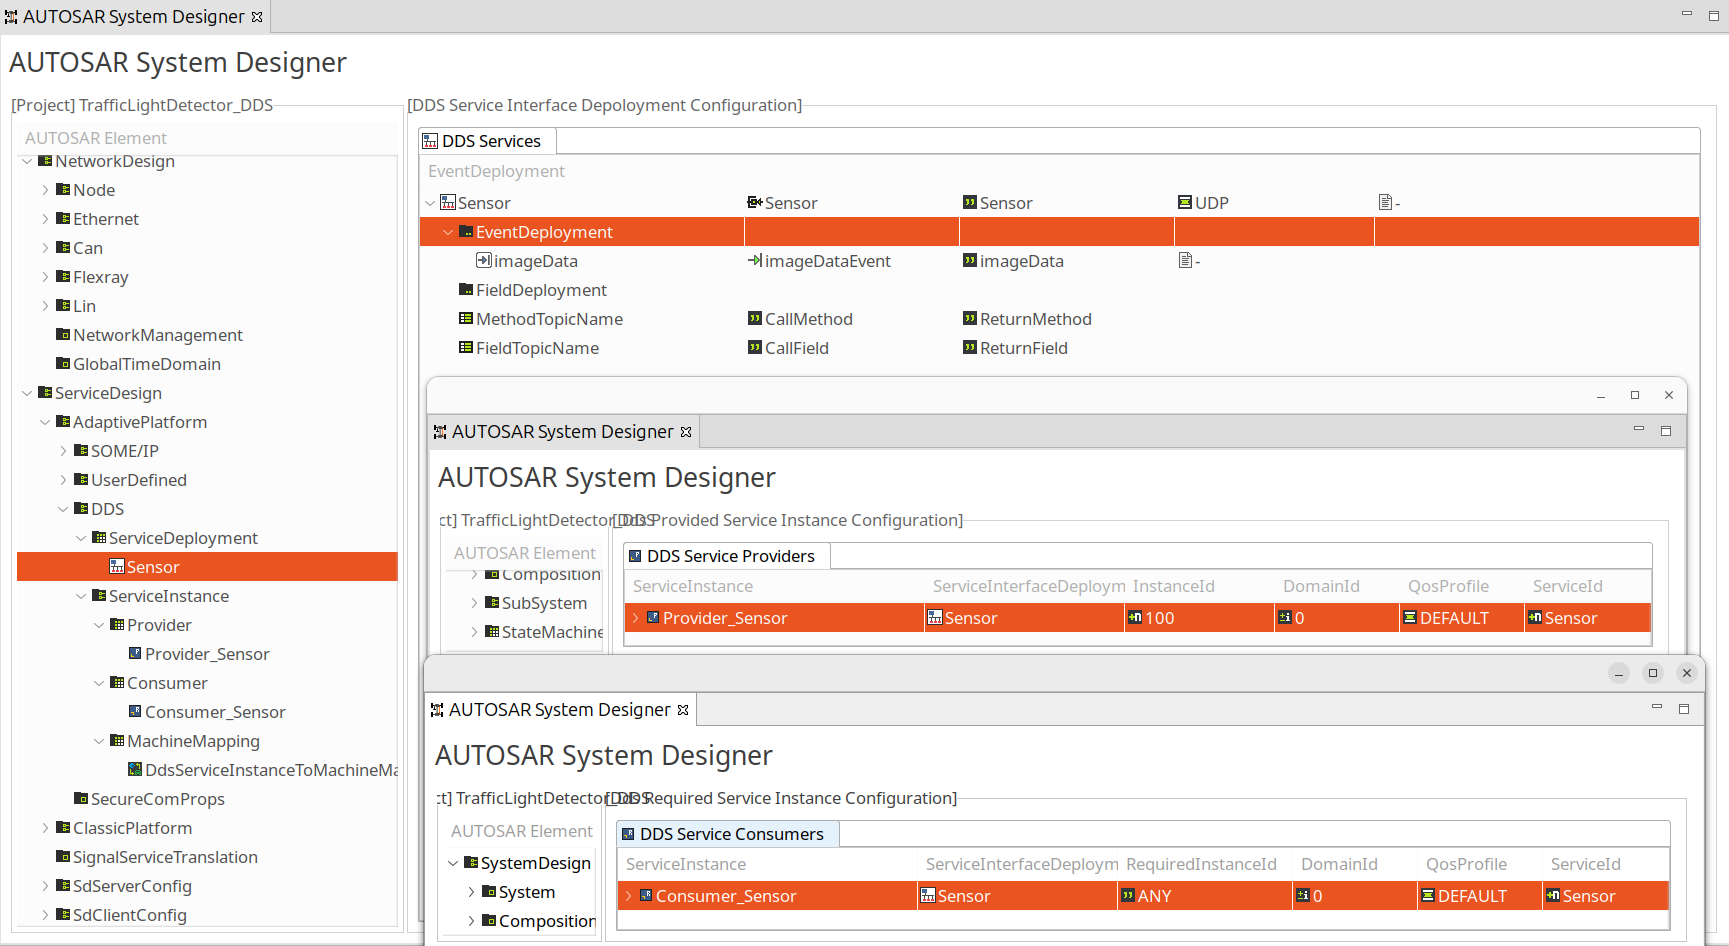
\includegraphics[width=0.75\textwidth]{Images/chap3/image_methodology/serviceInterfaceDesign/DDS_Config.png}
    \vspace{0.5cm}
    \caption{Mapping Service Instances to Machine Network Endpoint}
    \label{fig:dds_config}
\end{figure}

Similarly to the SOME/IP configuration, Figure~\ref{fig:dds_config} presents the DDS-based deployment configuration used for the \texttt{Sensor} service. In the DDS Service Interface Deployment Configuration, the service interface is deployed with the \texttt{imageDataEvent} event and the corresponding DDS topic \texttt{imageData}. The event deployment is configured to use UDP transport, allowing the Provider and Client applications to exchange image and metadata payloads through DDS publish/subscribe communication.

The provided service instance is configured as \texttt{Provider\_Sensor}, bound to the \texttt{Sensor} service deployment with instance-id~\texttt{100}, DDS Domain Id~\texttt{0}, and the \texttt{DEFAULT} QoS profile. The required service instance is configured as \texttt{Consumer\_Sensor}, also bound to the same \texttt{Sensor} service deployment, but with required instance-id~\texttt{ANY}. This configuration allows the Client application to discover and subscribe to the Provider service instance dynamically within the same DDS domain.

Through this DDS configuration, the abstract AUTOSAR service definition is mapped to concrete DDS communication entities, including service deployment, topic, event, provider instance, consumer instance, domain identifier, and QoS profile. This mapping is essential for the implemented prototype because the runtime communication between \texttt{ProviderSensor} and \texttt{ClientSensor} is realized through DDS rather than SOME/IP. As a result, the system can publish \texttt{imageDataEvent} samples on the \texttt{imageData} topic and deliver the \texttt{GpsJpegWireHeader + JPEG} payload from the Provider to the Client in a service-oriented and configurable manner.

\subsubsection{Application Design}

% Modeling Adaptive Application
\begin{figure}[H]
    \centering
    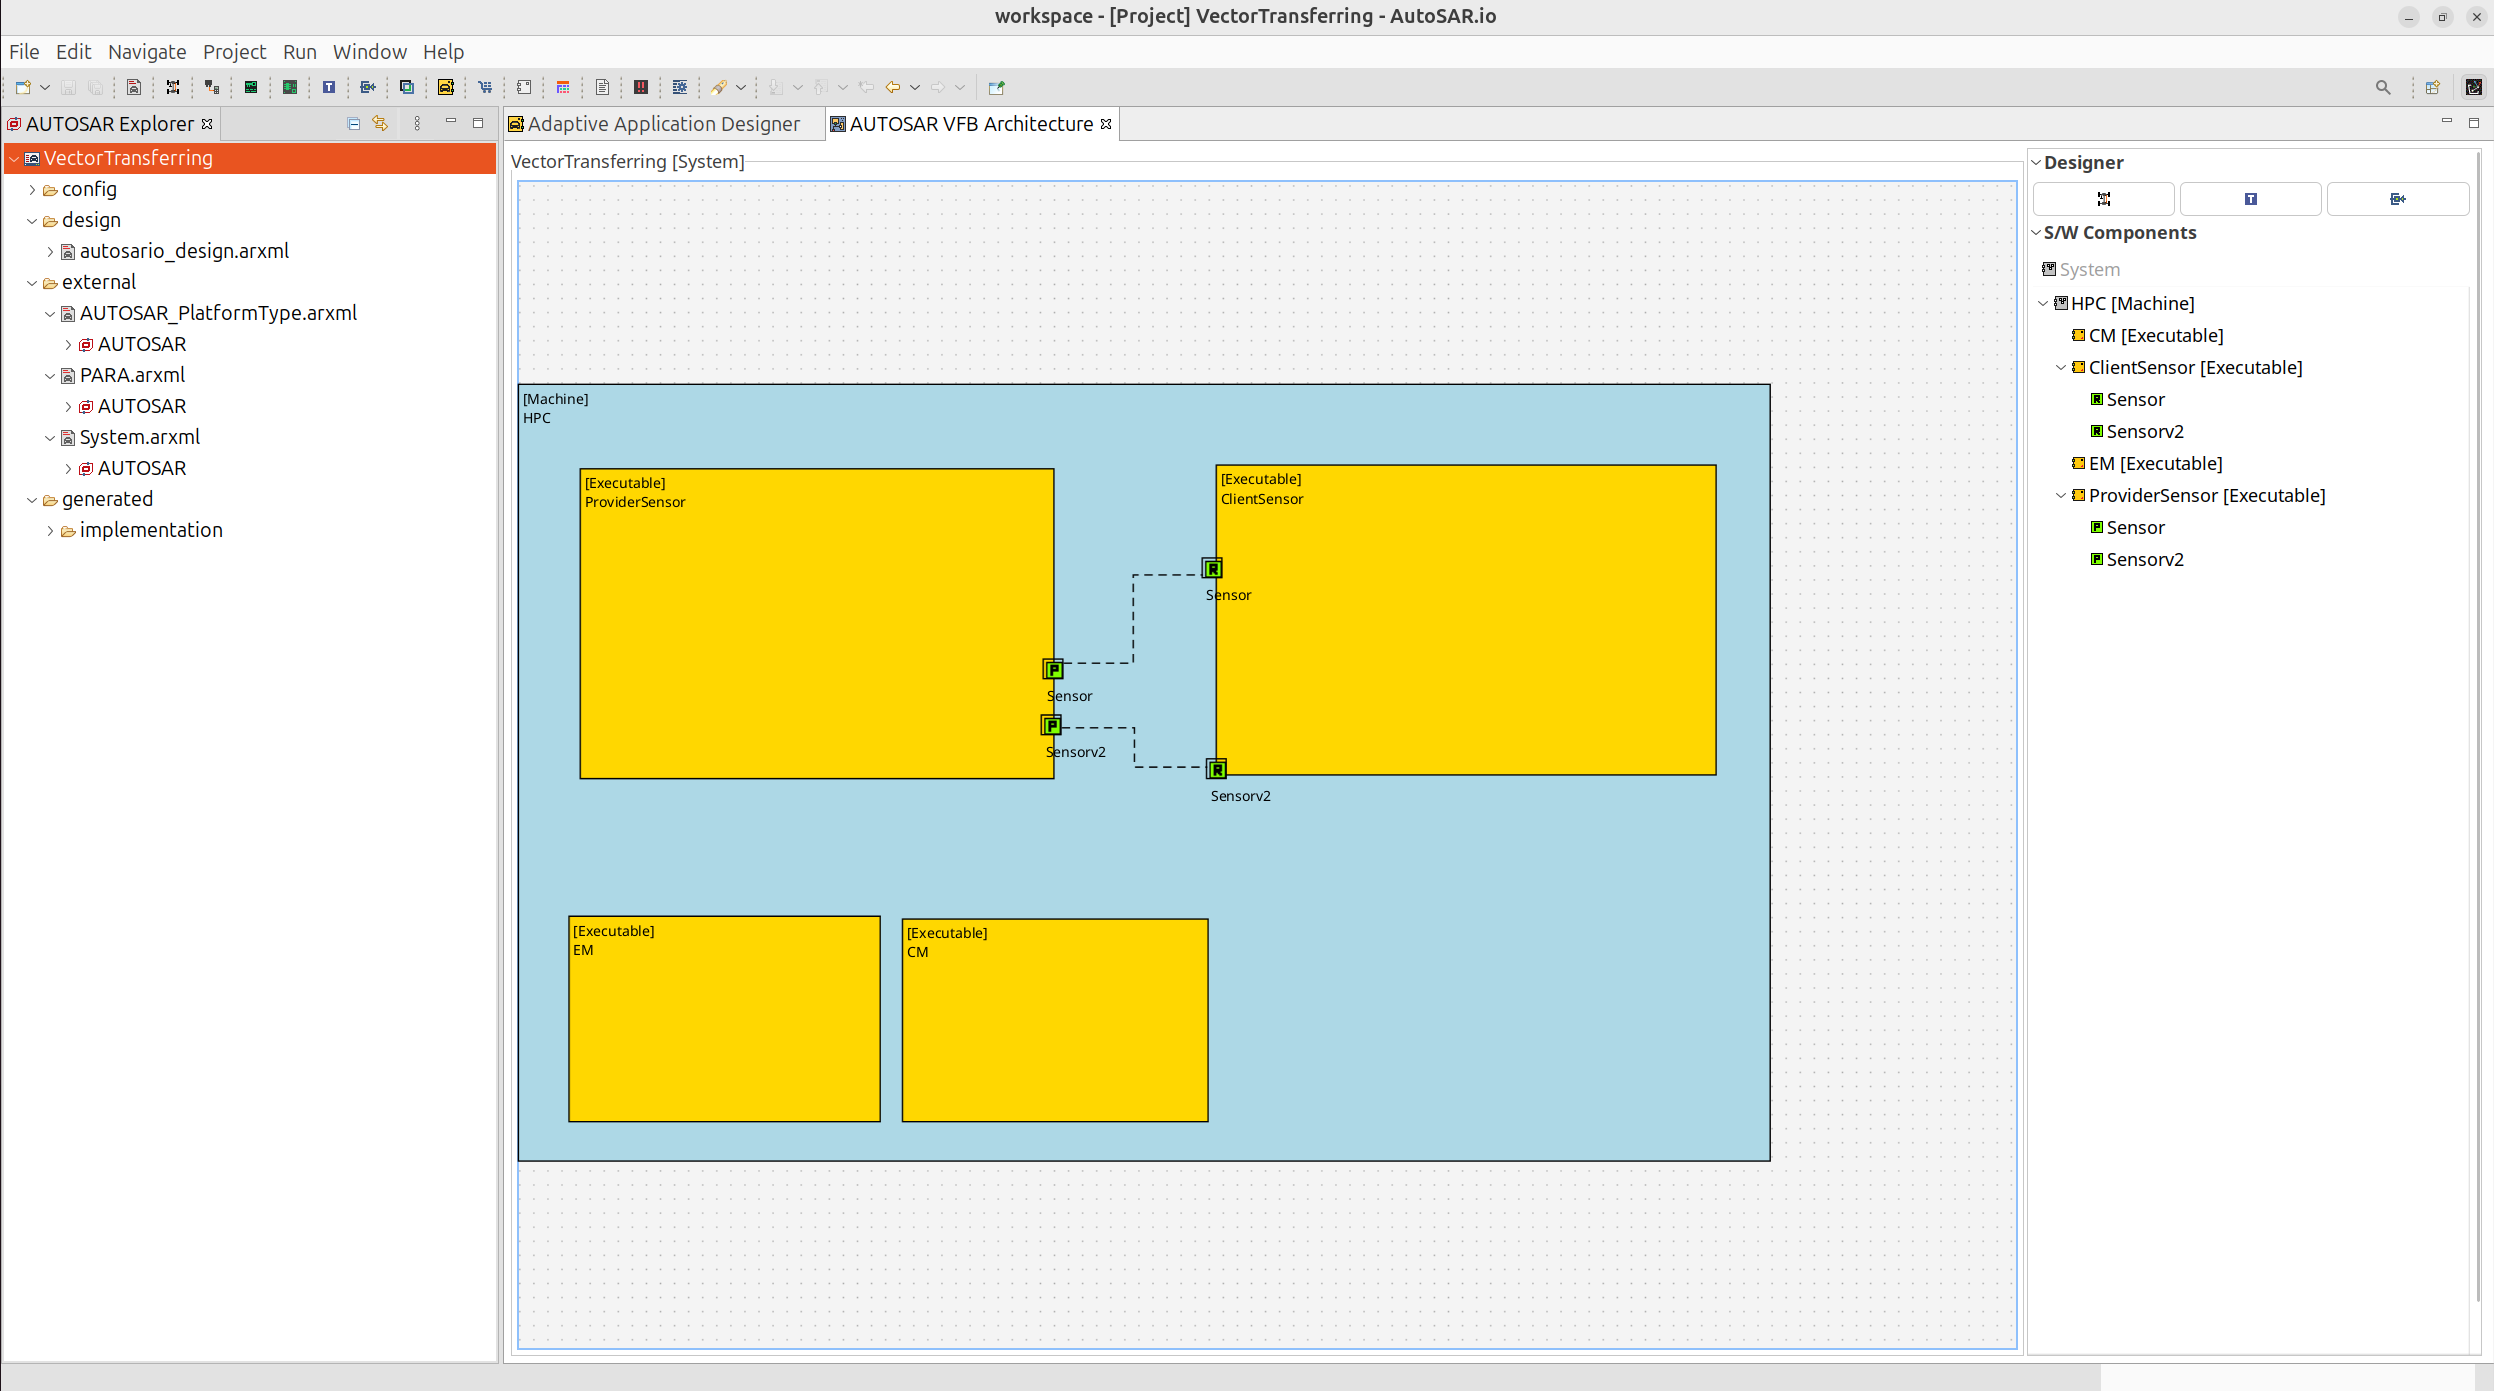
\includegraphics[width=0.75\textwidth]{Images/chap3/image_methodology/applicationDesign/modelingApplication.png}
    \vspace{0.5cm}
    \caption{Modeling of Adaptive Application}
    \label{fig:modeling_application}
\end{figure}

Figure~\ref{fig:modeling_application} shows the Adaptive Application modeling view, where users define the overall application architecture by assigning application executables to a specific machine. In this workspace, the target machine \texttt{HPC} is selected as the deployment context, and multiple executables such as \texttt{ProviderSensor}, \texttt{ClientSensor}, \texttt{CM}, and \texttt{EM} are instantiated within it. Logical connections between executables are visually represented through ports, allowing designers to describe interaction relationships at the architectural level. This model serves as a central design step that links application executables with the underlying machine, providing a clear and structured representation of how software components are organized and deployed in an Adaptive AUTOSAR system.


% Configure Provider Executable Properties
\begin{figure}[H]
    \centering
    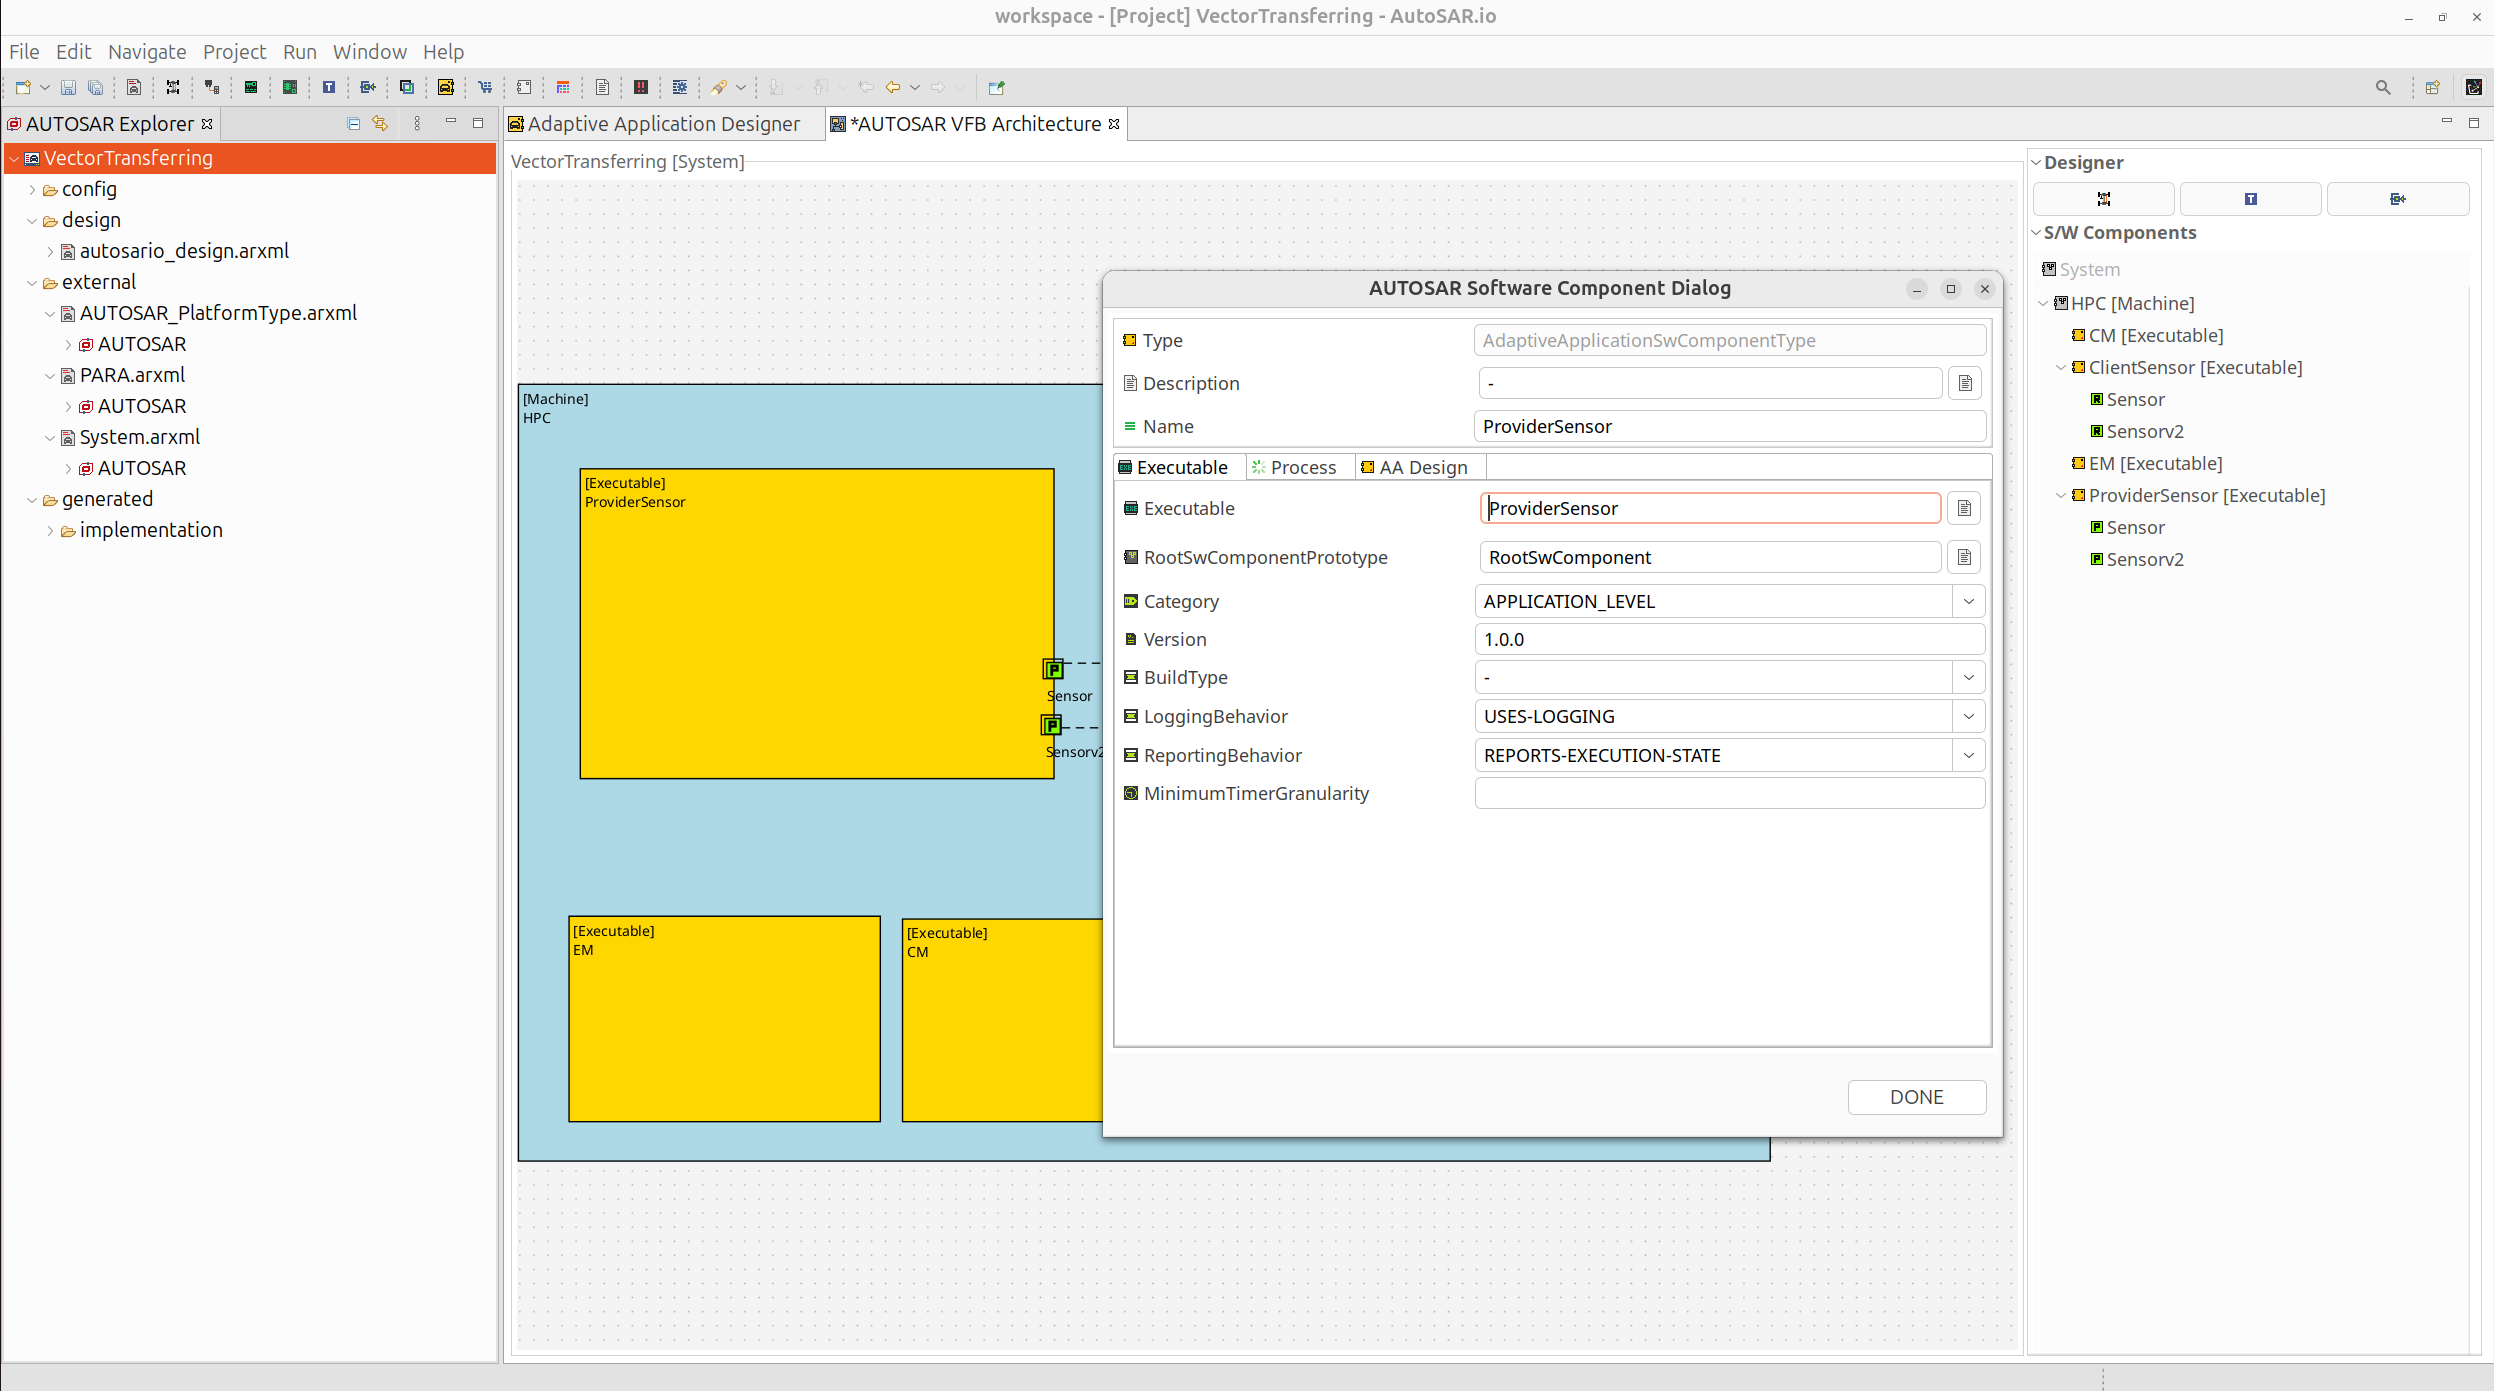
\includegraphics[width=0.75\textwidth]{Images/chap3/image_methodology/applicationDesign/providerExProperties.png}
    \vspace{0.5cm}
    \caption{Configuration of Provider Executable Properties}
    \label{fig:app_provider_executable_properties}
\end{figure}

Figure~\ref{fig:app_provider_executable_properties} presents the configuration of the provider application executable within the Adaptive Application Designer. In this view, the executable \texttt{ProviderSensor} is defined as an application level software component with a specific version and logging behavior. Key properties such as execution category, reporting behavior, and minimum timer granularity are configured to control runtime characteristics and observability. By assigning these attributes, the provider executable is clearly identified as a service offering entity and is prepared to integrate with the Adaptive AUTOSAR execution environment in a consistent and manageable manner.

% Map Provider Ports to Service Interface
\begin{figure}[H]
    \centering
    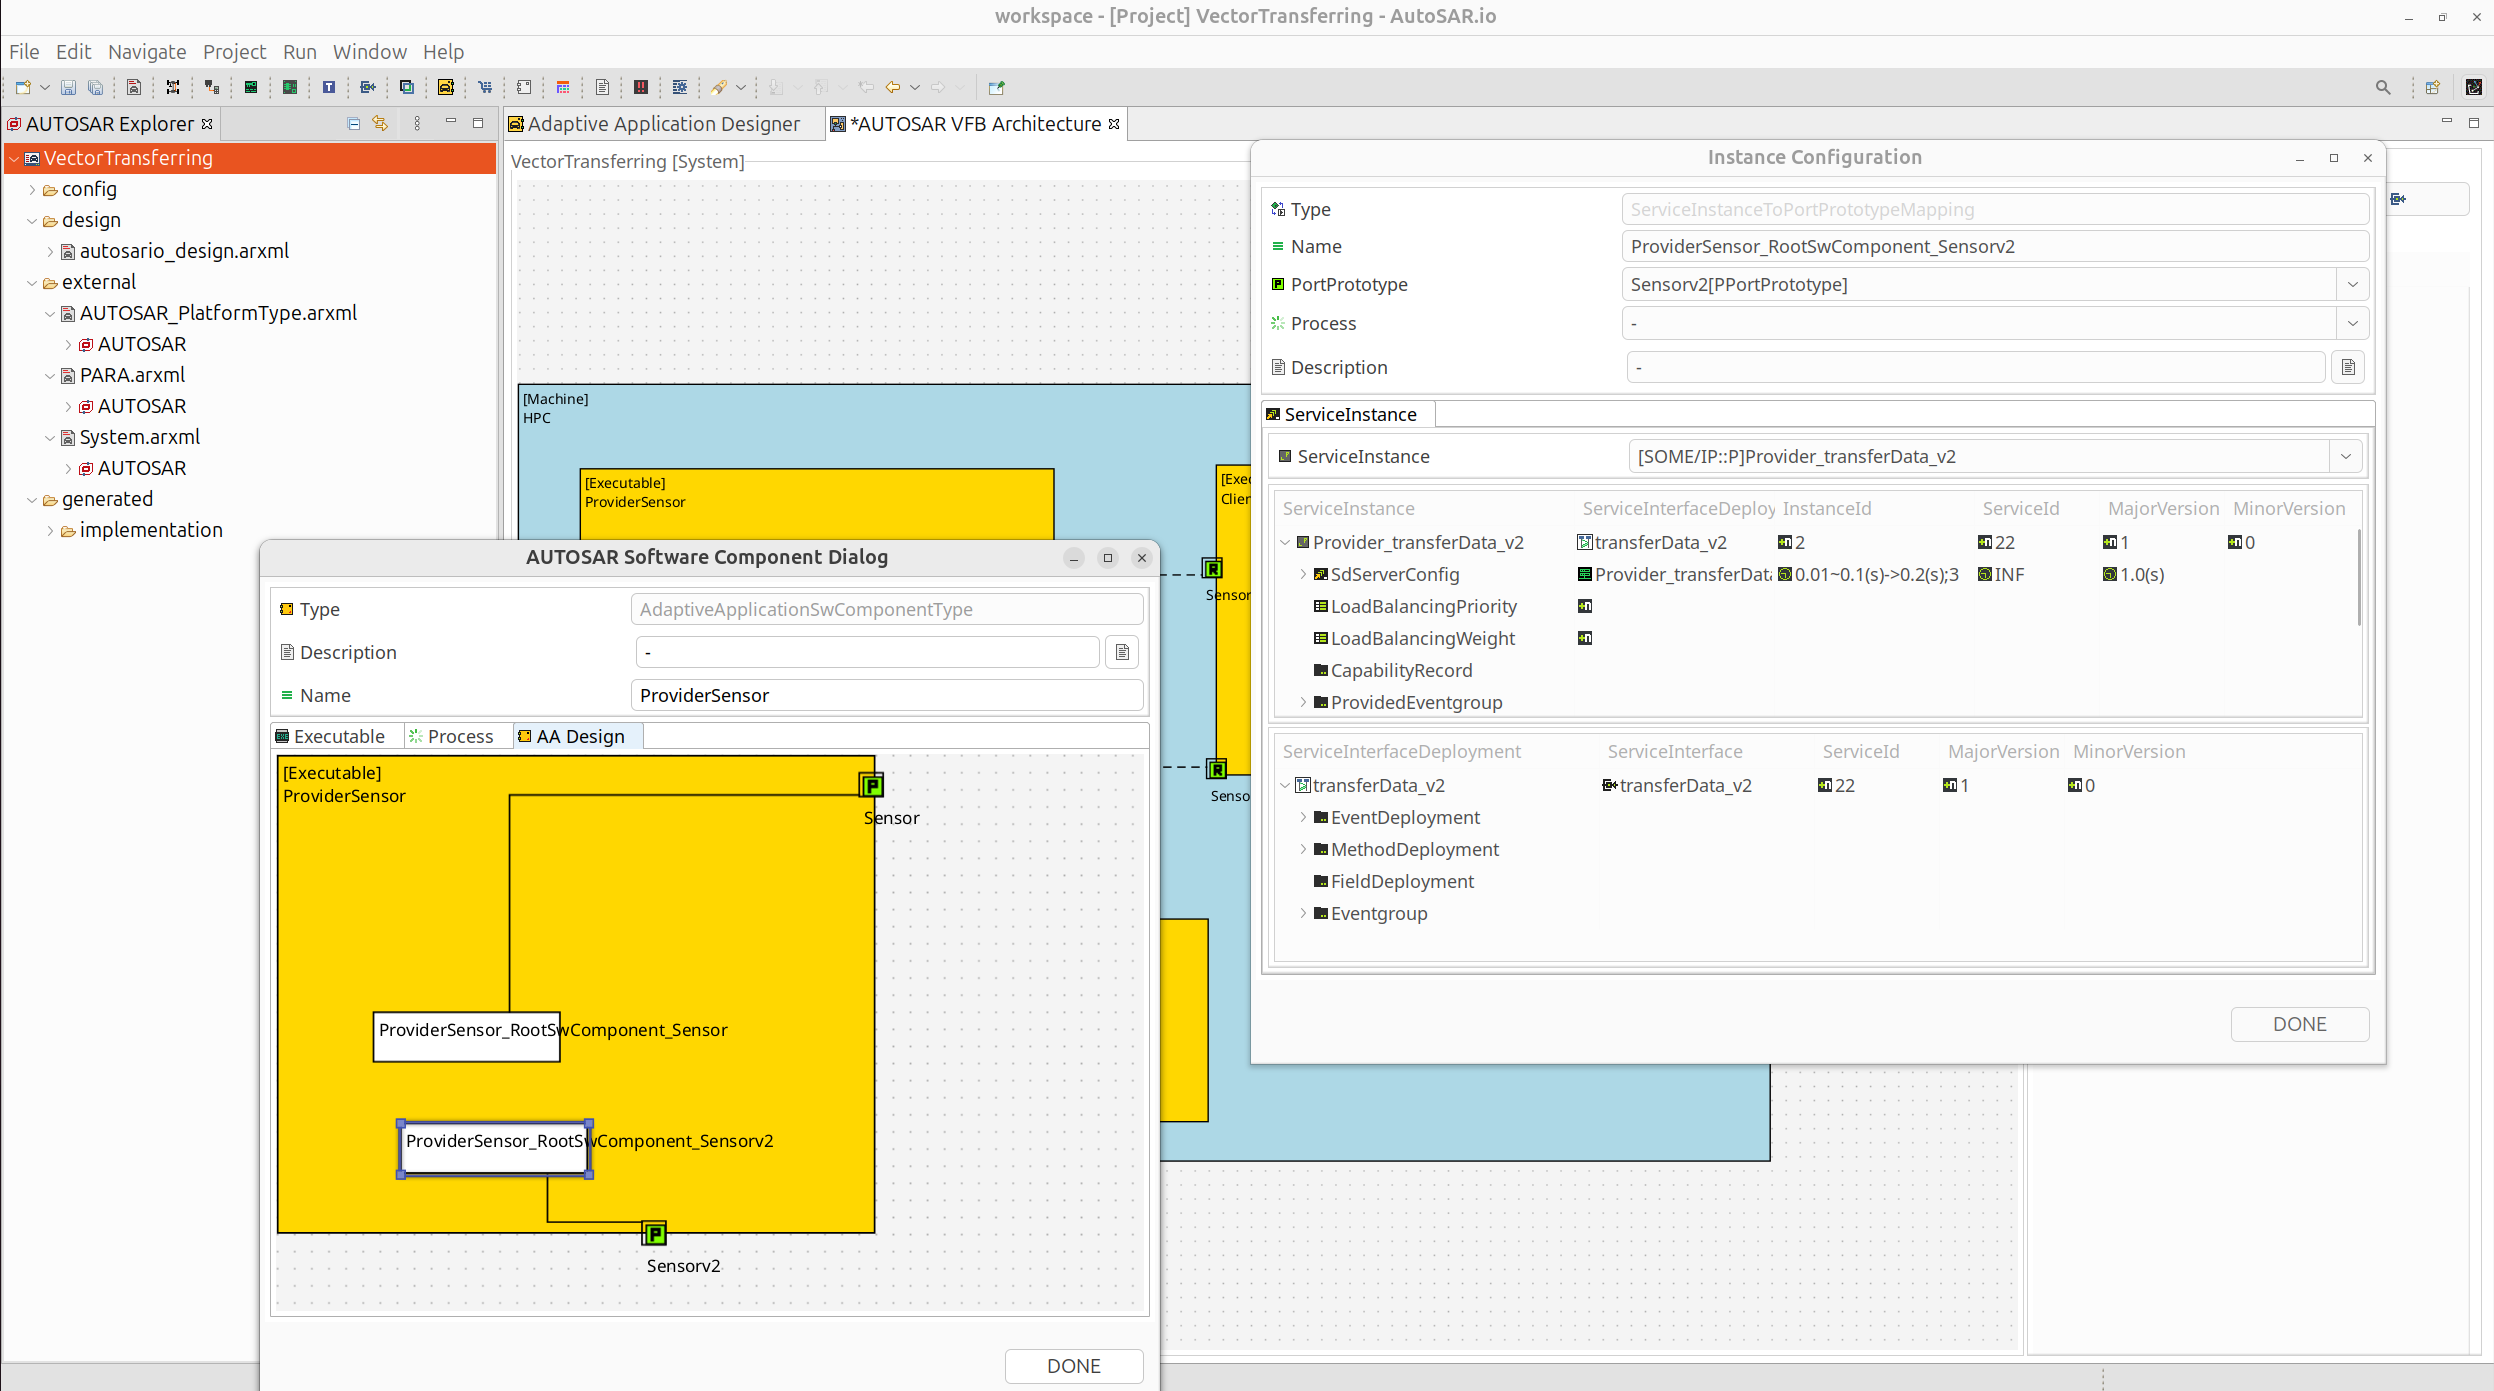
\includegraphics[width=0.75\textwidth]{Images/chap3/image_methodology/applicationDesign/mappingPortProviderEx.png}
    \vspace{0.5cm}
    \caption{Mapping Provider Ports to Service Interface}
    \label{fig:app_mapping_provider_ports}
\end{figure}

Figure~\ref{fig:app_mapping_provider_ports} illustrates the association between the provider executable ports and the previously defined AUTOSAR software component. In this step, the ports of the \texttt{ProviderSensor} executable are mapped to the corresponding port prototypes of the Adaptive Application Software Component that has already been specified in the AUTOSAR model. This configuration establishes a clear link between the executable instance and its software component definition, ensuring that the executable correctly realizes the component’s provided interfaces. As a result, the application implementation becomes consistent with the AUTOSAR architectural model before being bound to concrete service instances and communication middleware.


% Configure Subscriber Executable Properties
\begin{figure}[H]
    \centering
    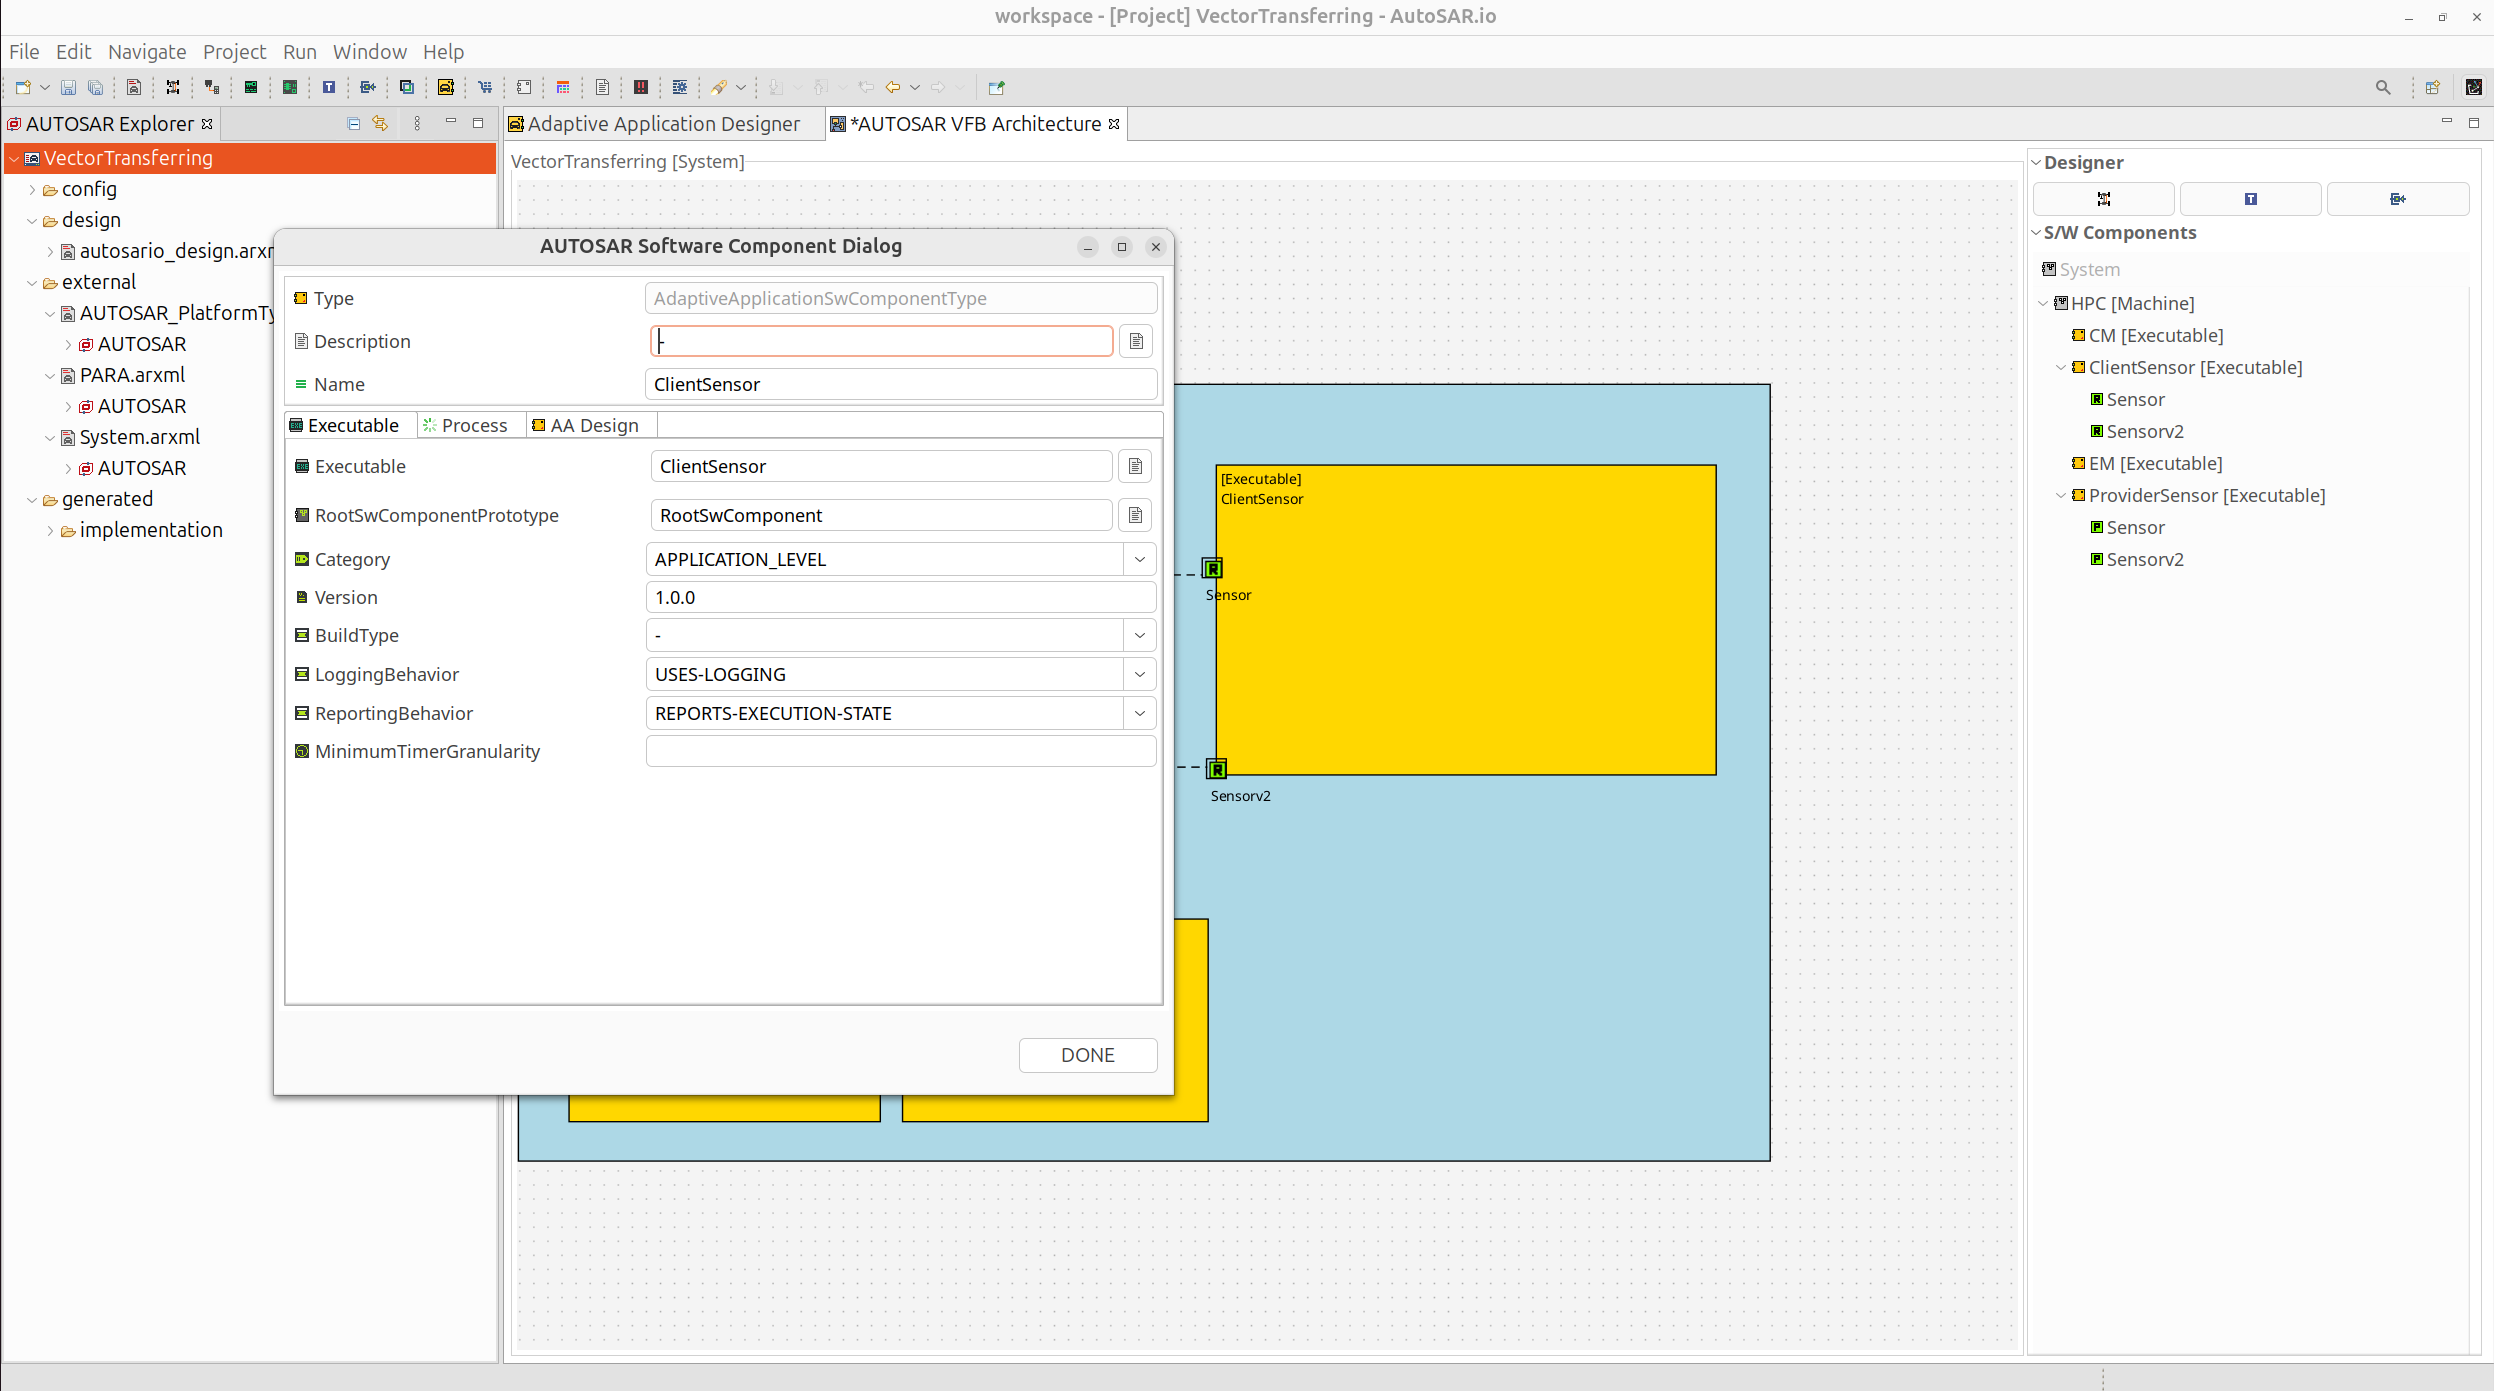
\includegraphics[width=0.75\textwidth]{Images/chap3/image_methodology/applicationDesign/subscriberExProperties.png}
    \vspace{0.5cm}
    \caption{Configuration of Subscriber Executable Properties}
    \label{fig:app_subscriber_executable_properties}
\end{figure}

Figure~\ref{fig:app_subscriber_executable_properties} illustrates the definition of the \texttt{ClientSensor} executable as an adaptive application software component. In this step, the executable is characterized at the application level by specifying its name, version, category, and runtime behavior such as logging and execution state reporting. This configuration formally registers the client application in the AUTOSAR model and establishes it as a runnable entity that can participate in service oriented communication.

% Map Client Ports to Service Interface
\begin{figure}[H]
    \centering
    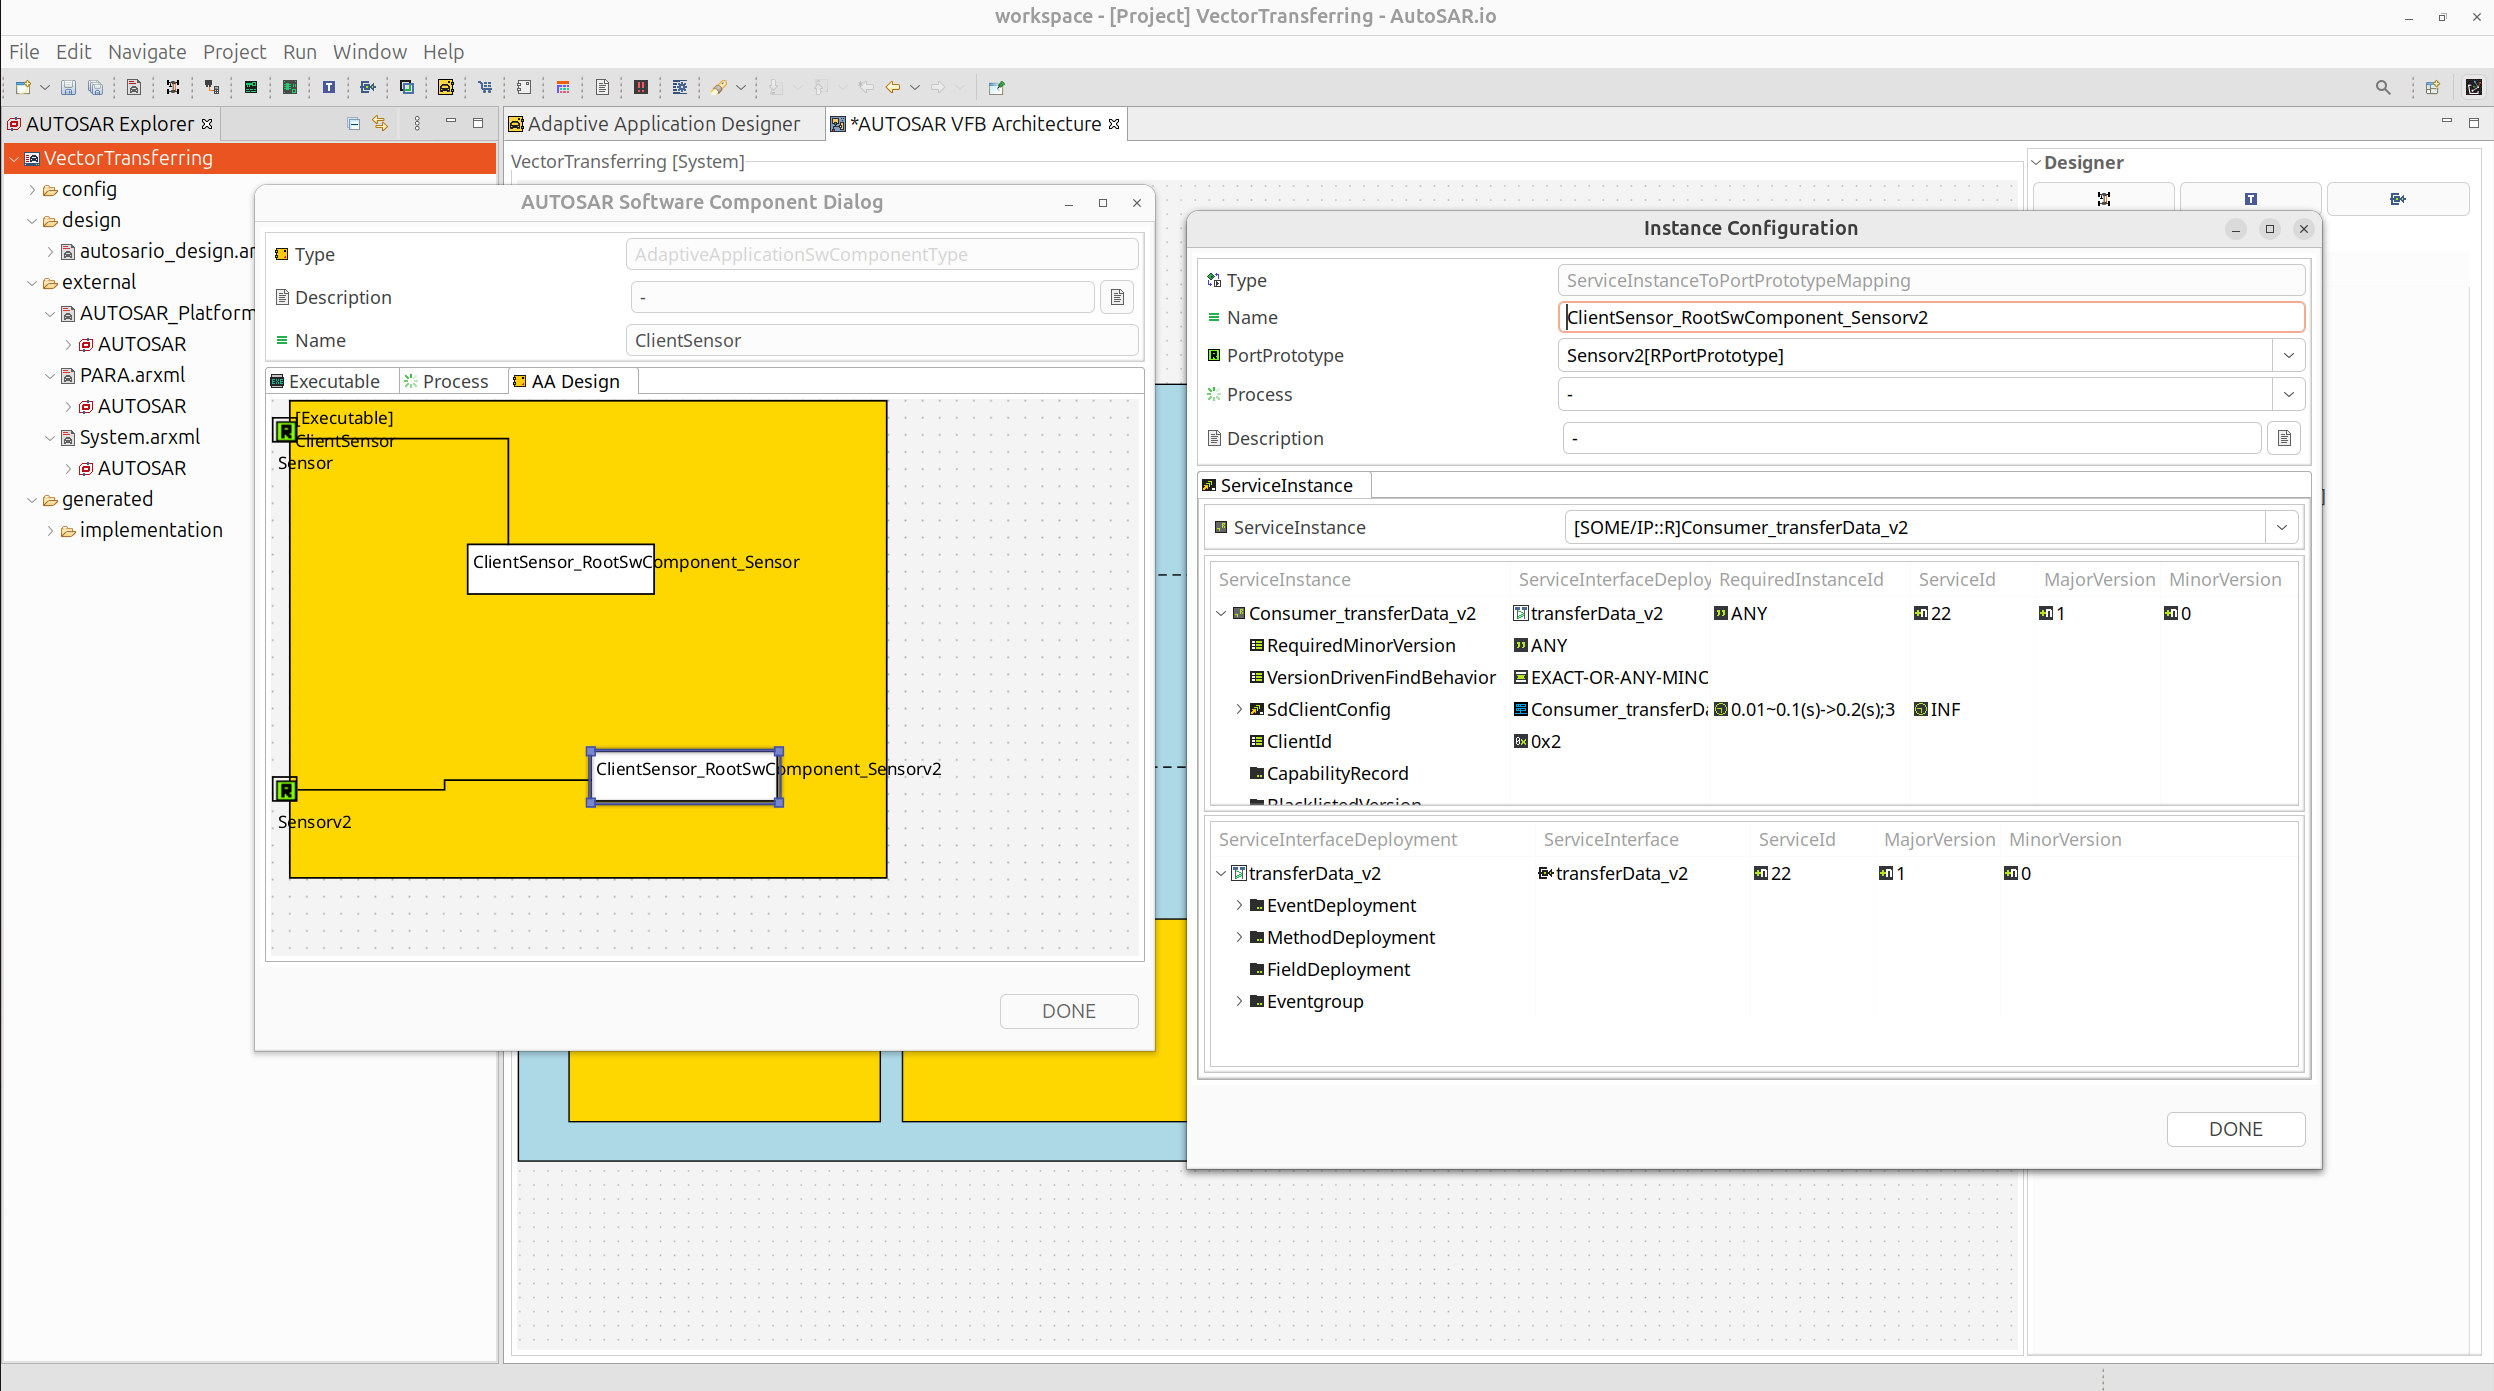
\includegraphics[width=0.75\textwidth]{Images/chap3/image_methodology/applicationDesign/mappingPortClientEx.png}
    \vspace{0.5cm}
    \caption{Mapping Client Ports to Service Interface}
    \label{fig:app_mapping_client_ports}
\end{figure}

As shown in Figure~\ref{fig:app_mapping_client_ports}, the required ports of the \texttt{ClientSensor} software component are then associated with the corresponding port prototypes defined in the AUTOSAR architecture. This association links the client implementation to the abstract interface contracts specified at design time, without directly binding it to network level details. By completing this step, the client executable is structurally aligned with the AUTOSAR software component model, enabling subsequent binding to concrete service instances during service deployment and machine mapping.

% Configure Application Startup Behavior
\begin{figure}[H]
    \centering
    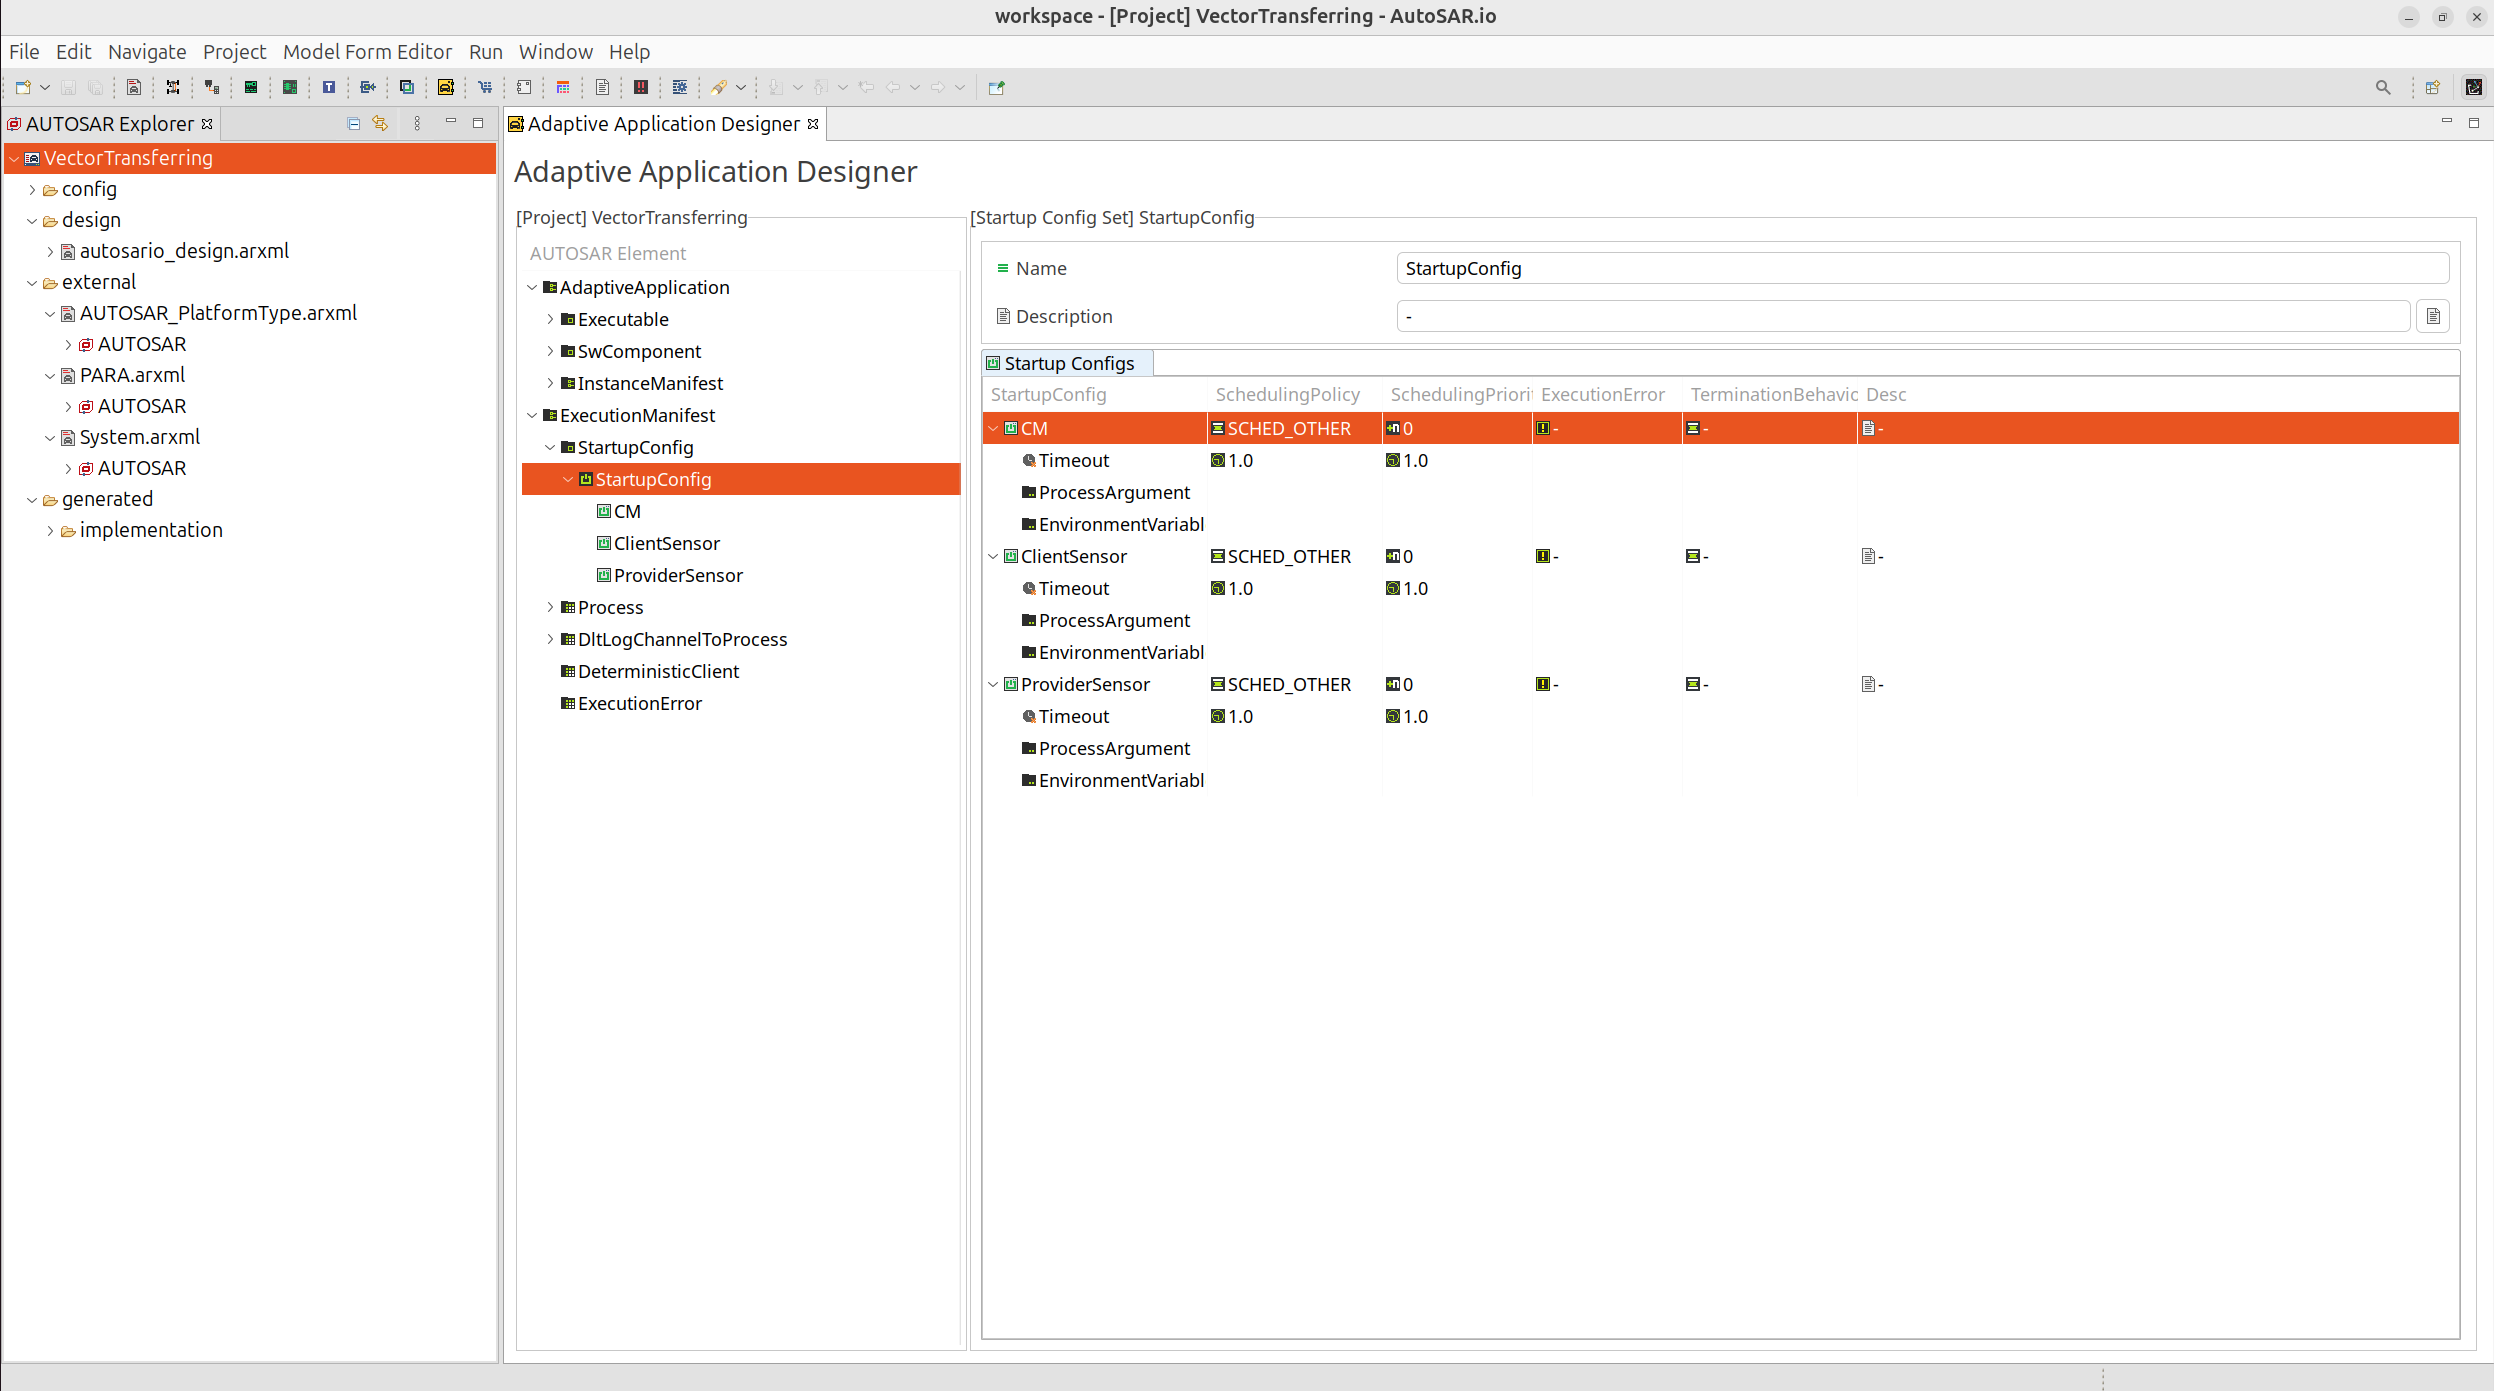
\includegraphics[width=0.75\textwidth]{Images/chap3/image_methodology/applicationDesign/configureStartupConfigure.png}
    \vspace{0.5cm}
    \caption{Configuration of Application Startup Behavior}
    \label{fig:app_startup_configuration}
\end{figure}

Figure~\ref{fig:app_startup_configuration} illustrates the startup configuration set that governs how adaptive application processes are initialized on the target platform. Each process, including \texttt{CM}, \texttt{ClientSensor}, and \texttt{ProviderSensor}, is assigned a scheduling policy and priority, ensuring consistent execution behavior under the POSIX based operating environment. The use of a unified scheduling class allows the platform to manage multiple applications in a predictable manner during system boot.

In addition, the startup configuration defines timeout values and process level parameters that control execution supervision at launch time. By explicitly specifying these attributes, the system ensures that all applications enter a well defined initial state and comply with platform execution constraints. This configuration plays a critical role in coordinating application startup with function group transitions and provides a stable foundation for subsequent runtime interactions.

% Bind DLT Channels to Application Processes
\begin{figure}[H]
    \centering
    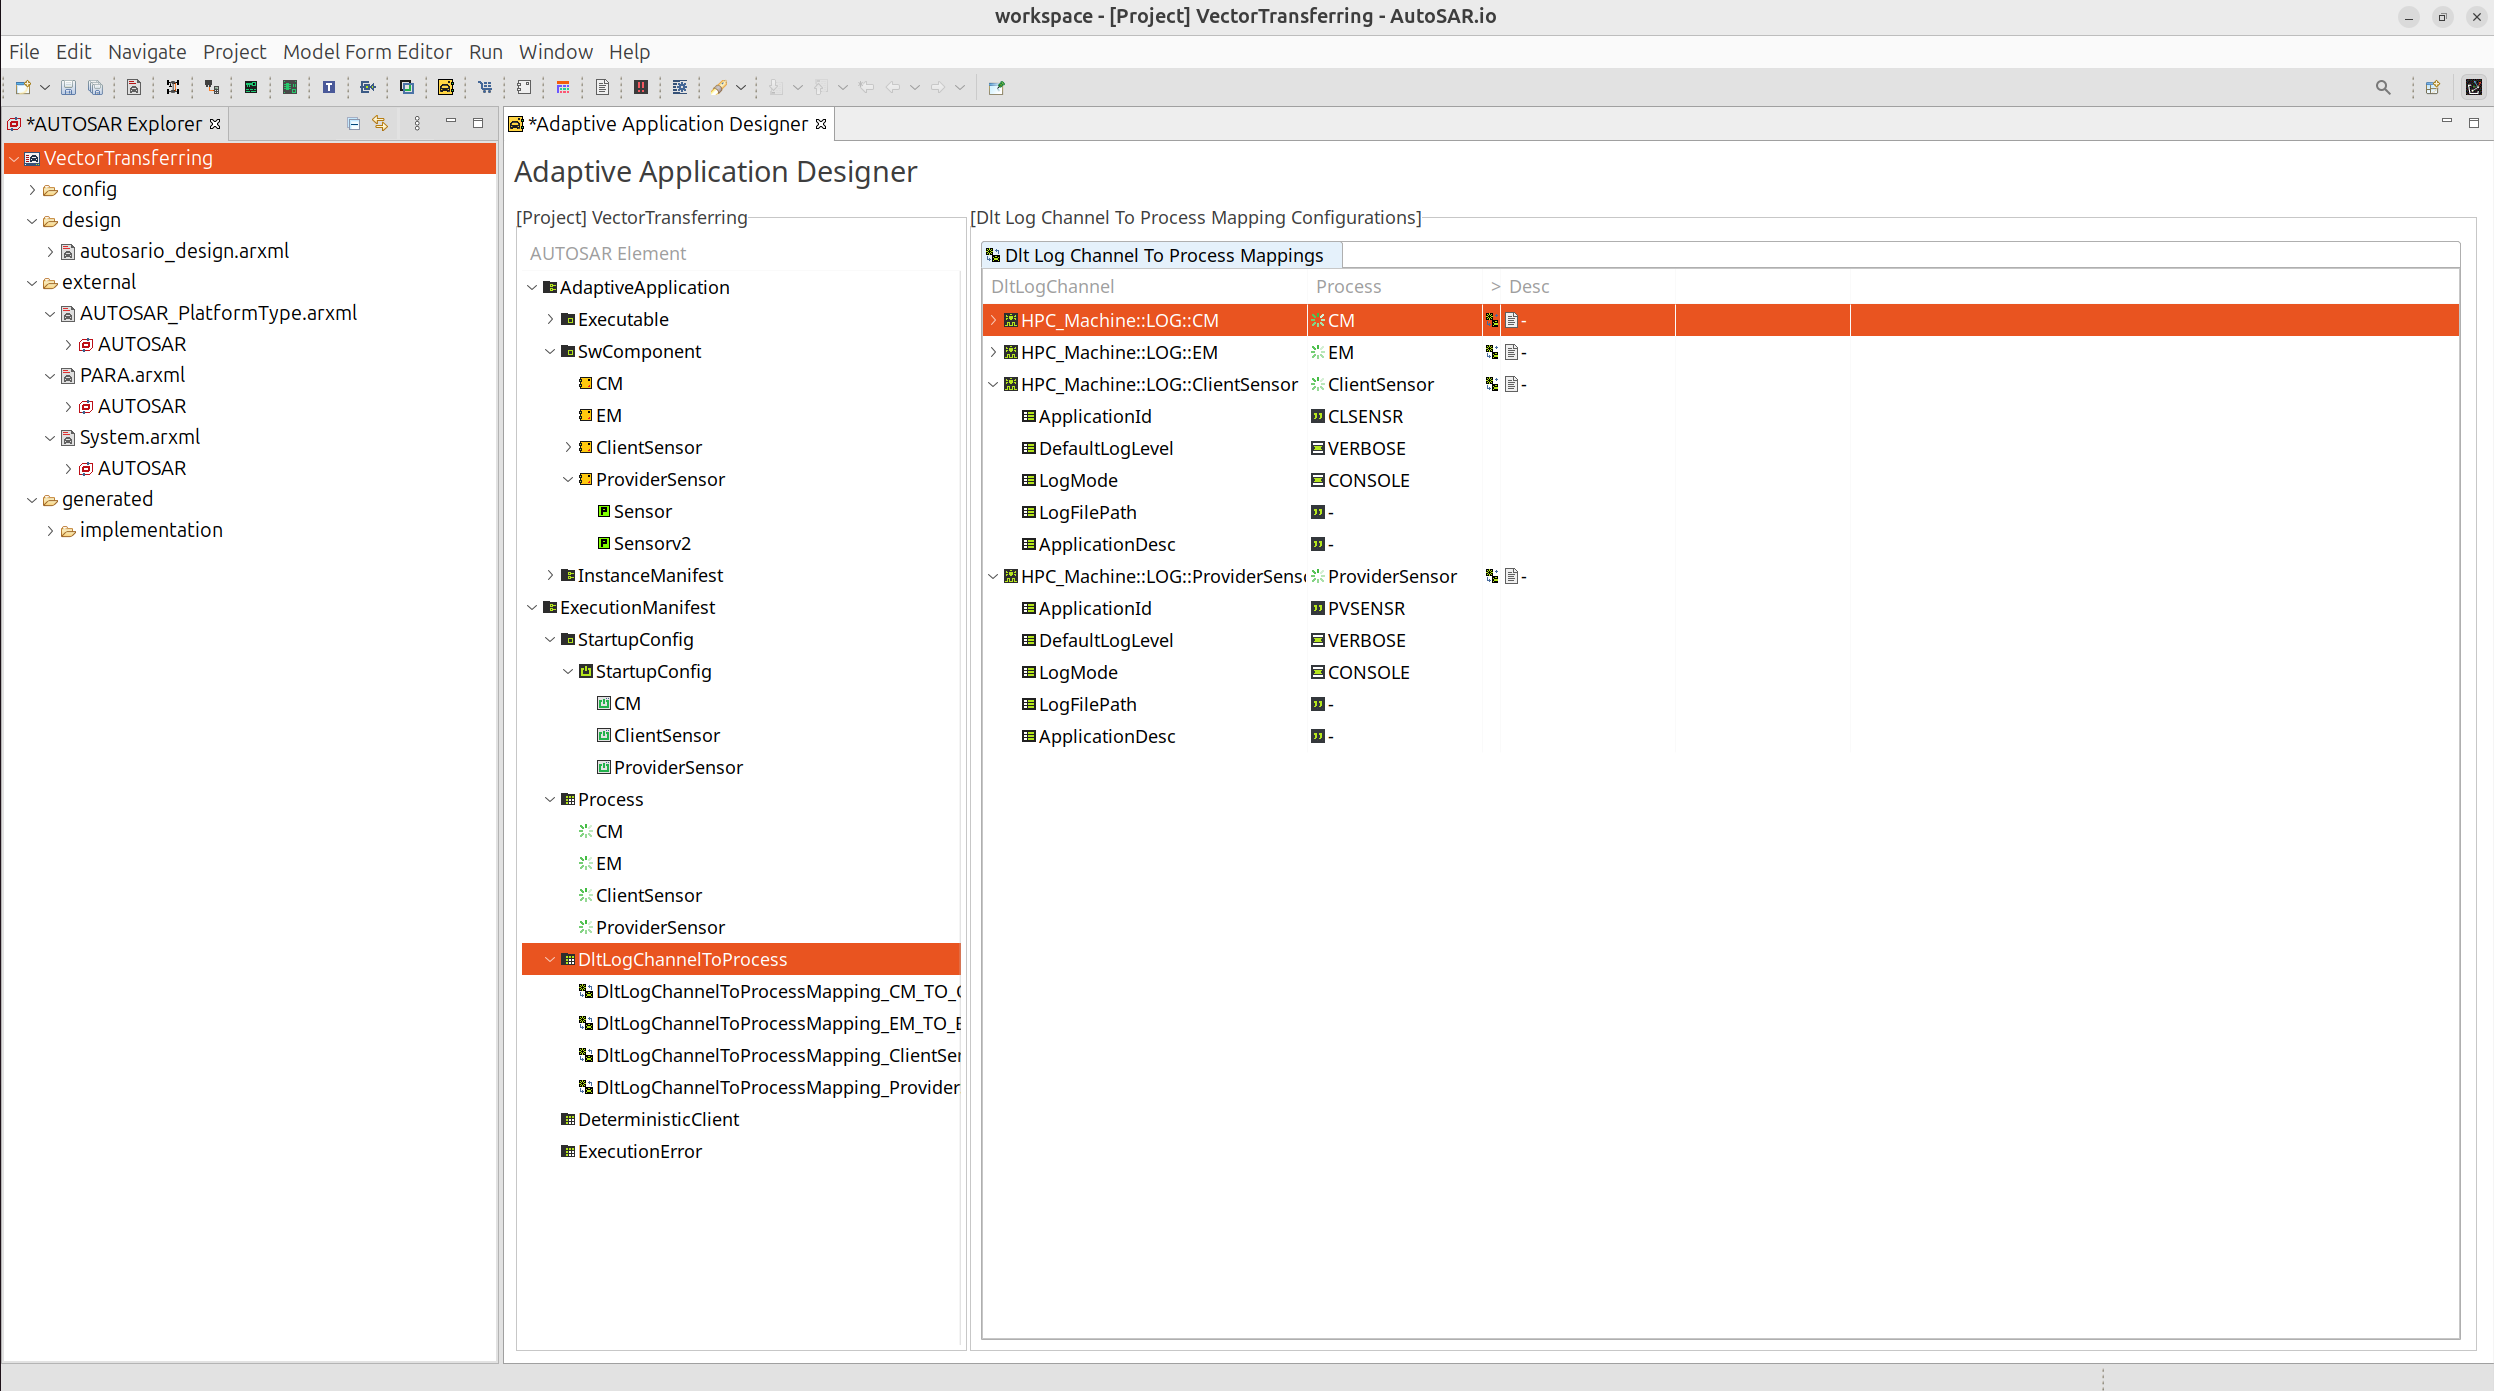
\includegraphics[width=0.75\textwidth]{Images/chap3/image_methodology/applicationDesign/configureDLTChanneltoProcess.png}
    \vspace{0.5cm}
    \caption{Binding Diagnostic Log and Trace Channels to Application Processes}
    \label{fig:app_dlt_process_mapping}
\end{figure}

Figure~\ref{fig:app_dlt_process_mapping} depicts the association between Diagnostic Log and Trace channels and individual application processes. Each process is connected to a specific DLT channel with defined log levels and output modes, enabling consistent monitoring and debugging at runtime. This mapping ensures that diagnostic information is traceable per application, which supports efficient analysis and maintenance in Adaptive AUTOSAR deployments.

% Configure Provider Application Process
\begin{figure}[H]
    \centering
    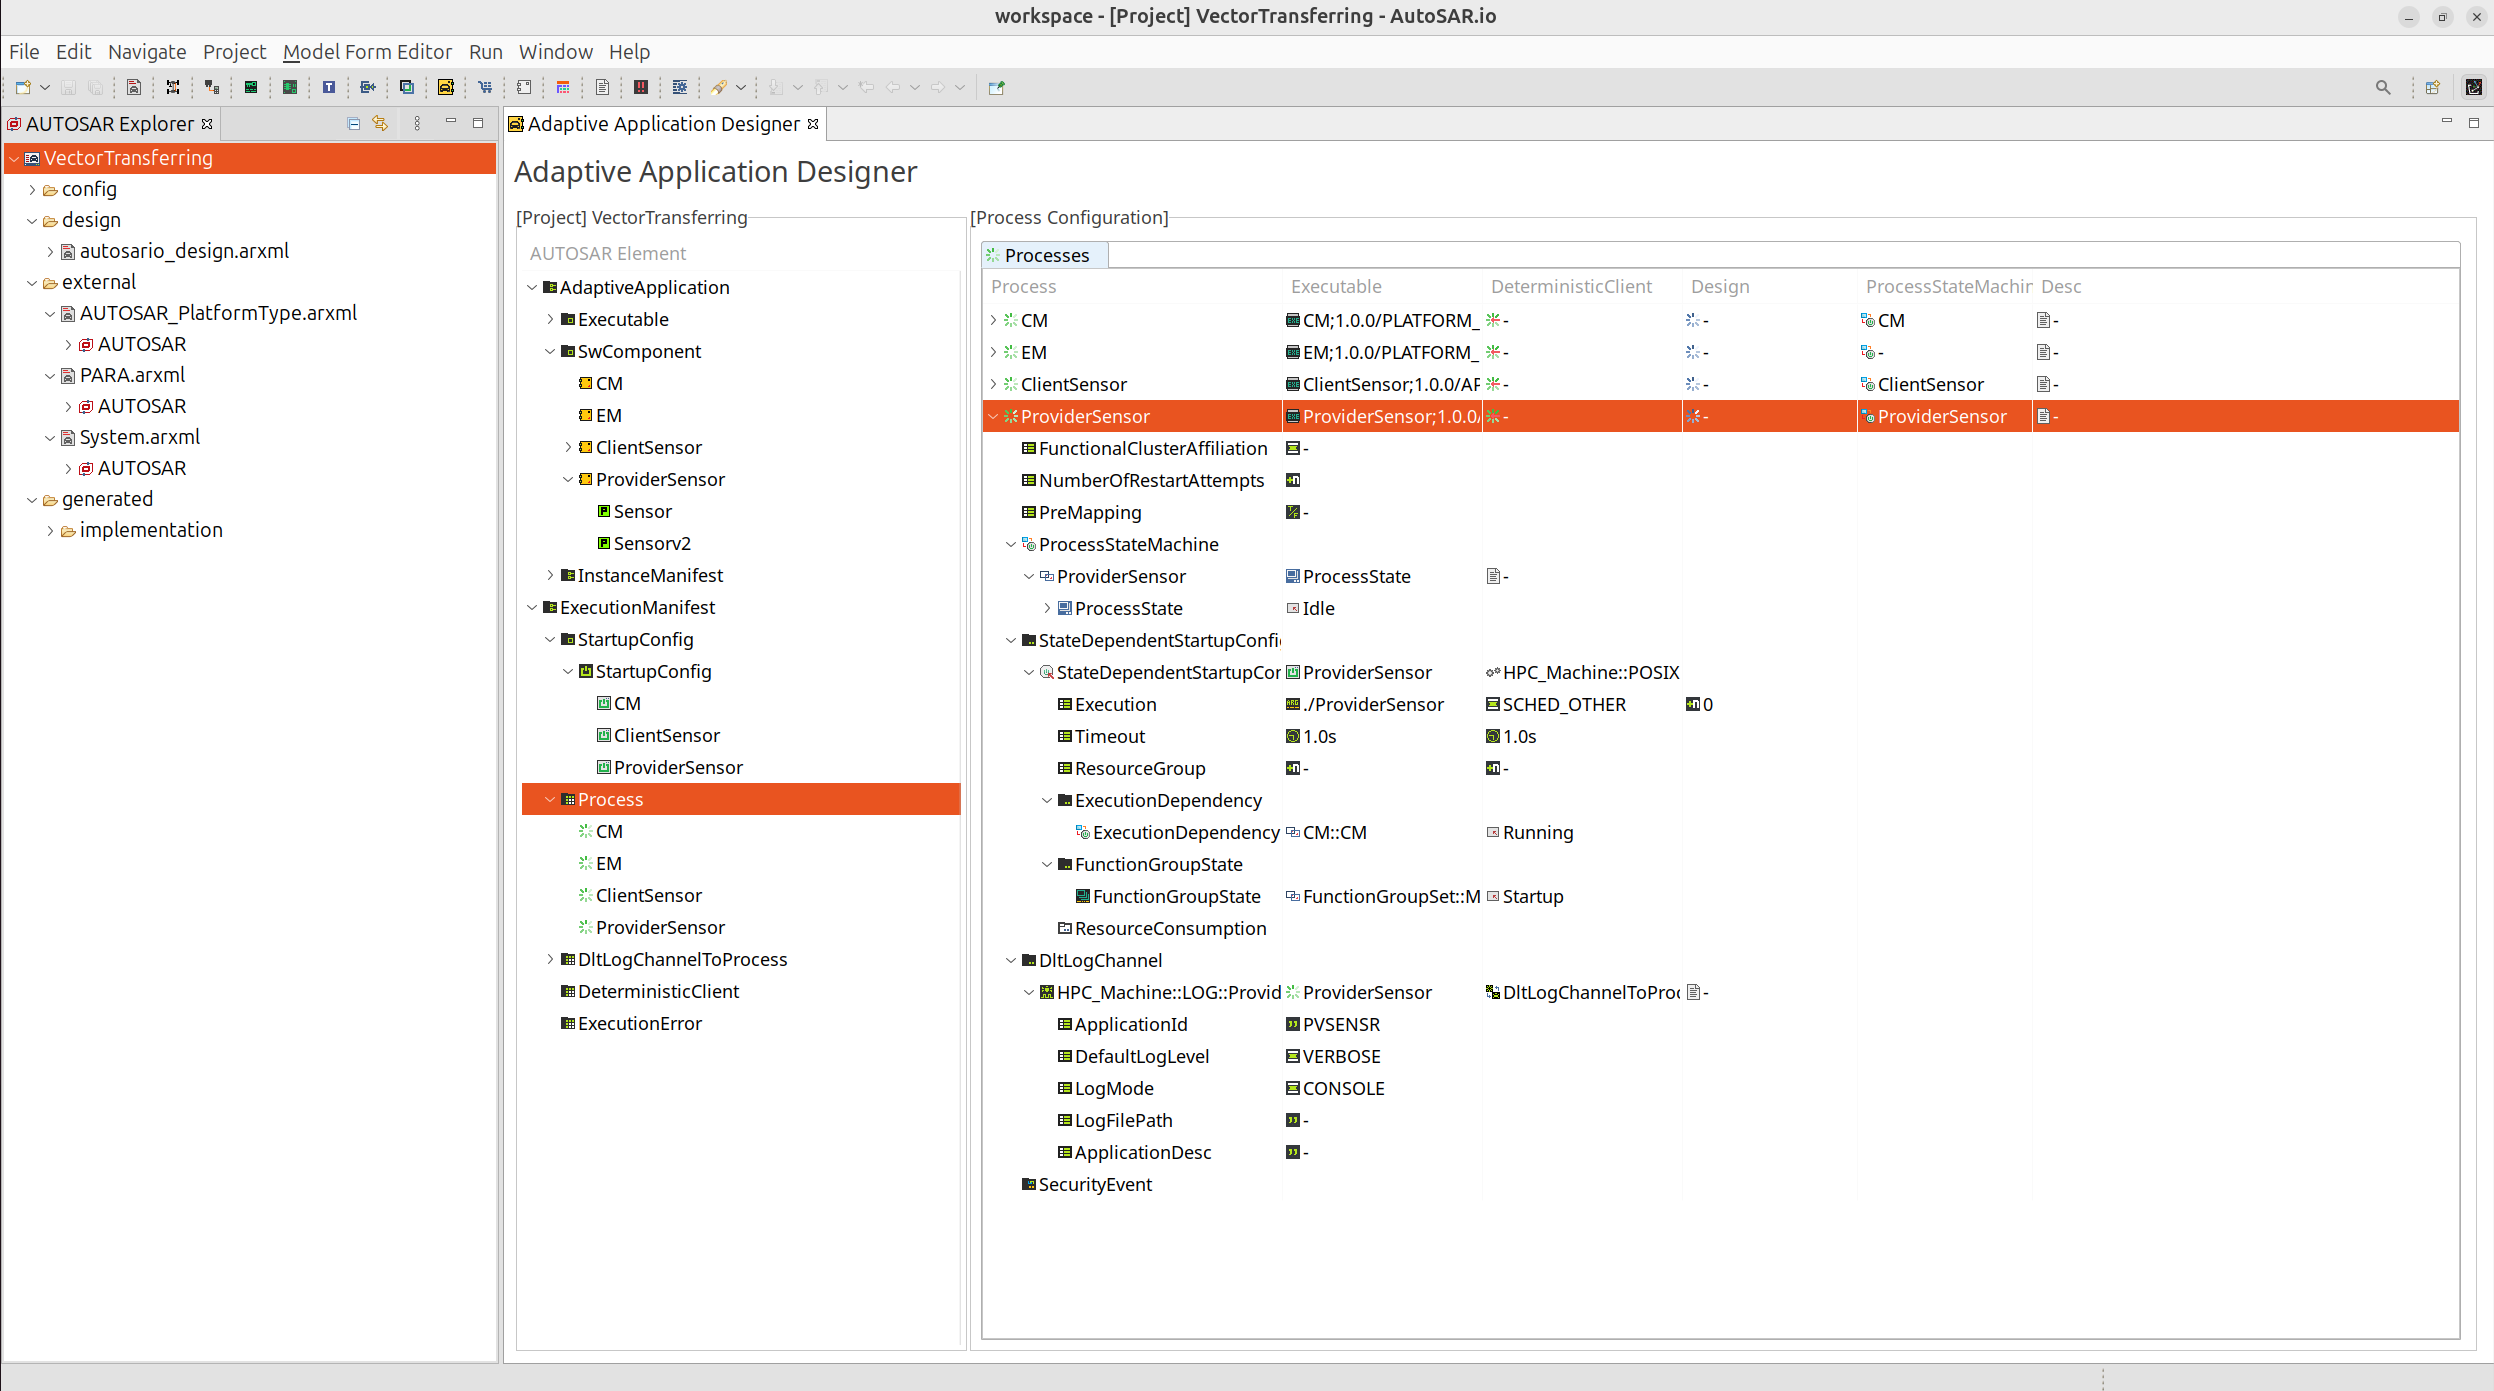
\includegraphics[width=0.75\textwidth]{Images/chap3/image_methodology/applicationDesign/configureProviderProcess.png}
    \vspace{0.5cm}
    \caption{Configuration of Provider Application Process}
    \label{fig:app_provider_process_configuration}
\end{figure}

As illustrated in Figure~\ref{fig:app_provider_process_configuration}, the provider application process is configured by linking the \texttt{ProviderSensor} executable to a dedicated process entity. This step specifies process level attributes such as restart policy, execution dependency, and state machine association, which together describe how the provider behaves during runtime transitions. The configuration clarifies the provider’s role in the execution flow and its dependency on platform level services.

% Configure Client Application Process
\begin{figure}[H]
    \centering
    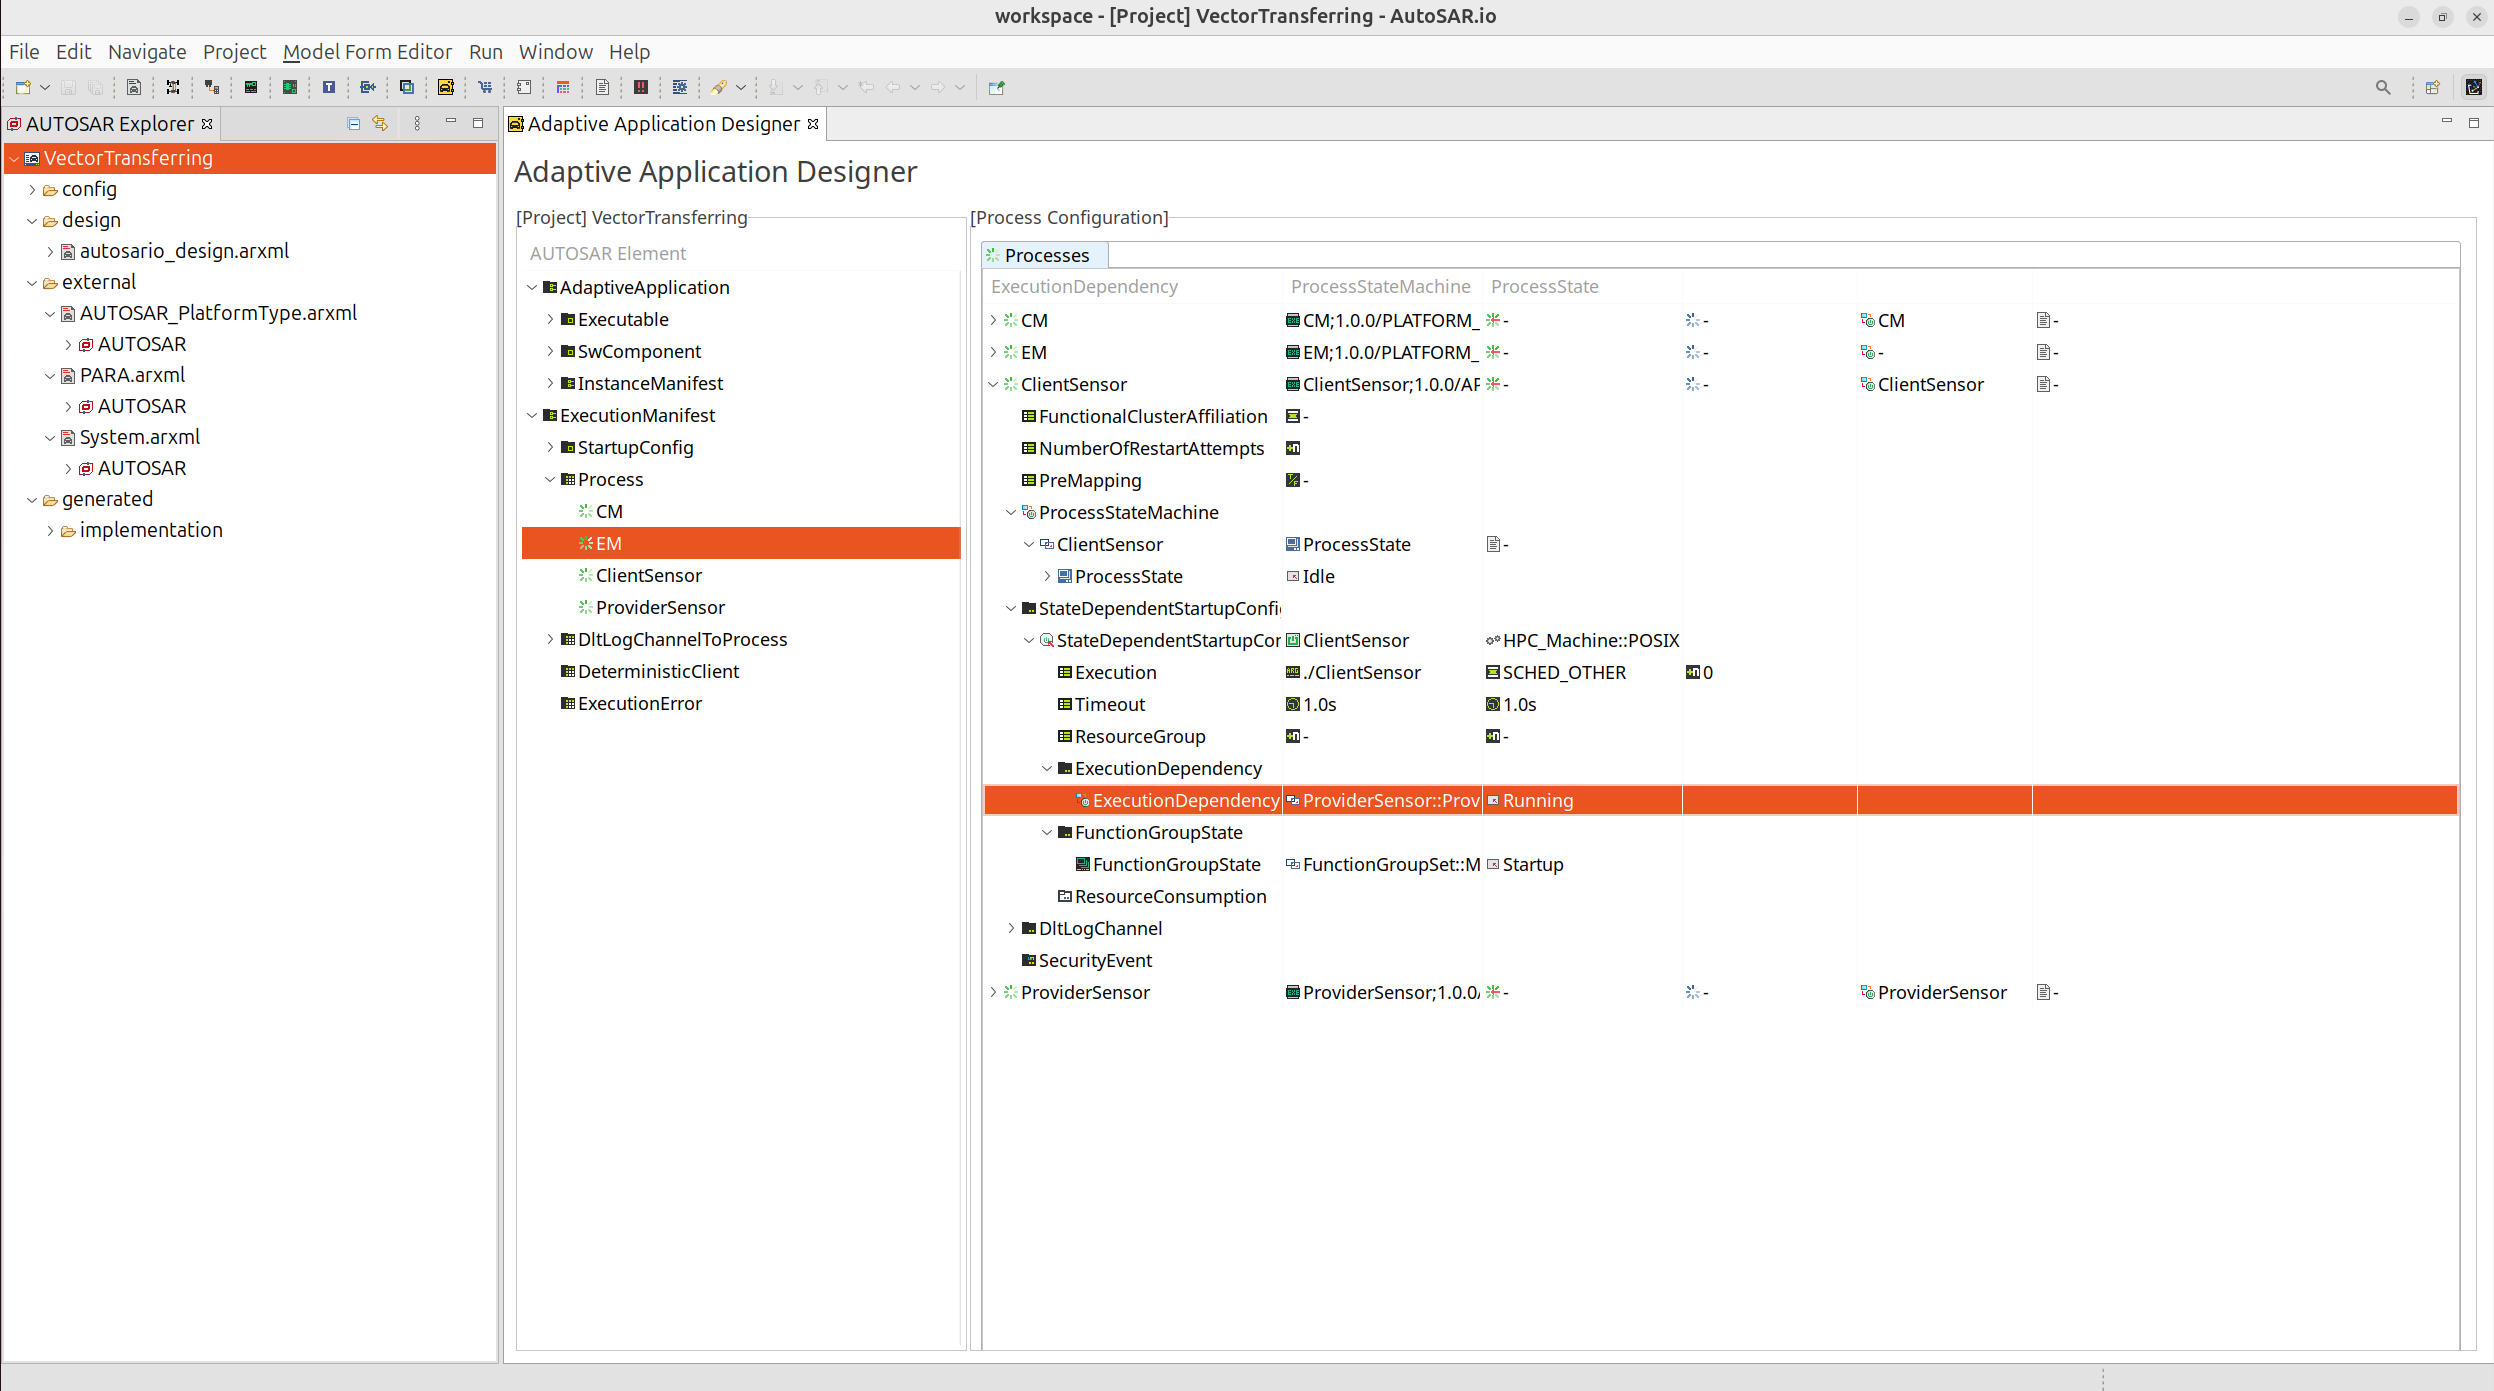
\includegraphics[width=0.75\textwidth]{Images/chap3/image_methodology/applicationDesign/configureClientProcess.png}
    \vspace{0.5cm}
    \caption{Configuration of Client Application Process}
    \label{fig:app_client_process_configuration}
\end{figure}

Figure~\ref{fig:app_client_process_configuration} shows a similar setup for the client application, where the \texttt{ClientSensor} executable is bound to its own process instance. Here, execution states and startup dependencies are defined to ensure that the client is activated only when required conditions are satisfied. This separation at the process level improves modularity and allows independent management of client and provider lifecycles.

% Map Application Processes to Target Machine
\begin{figure}[H]
    \centering
    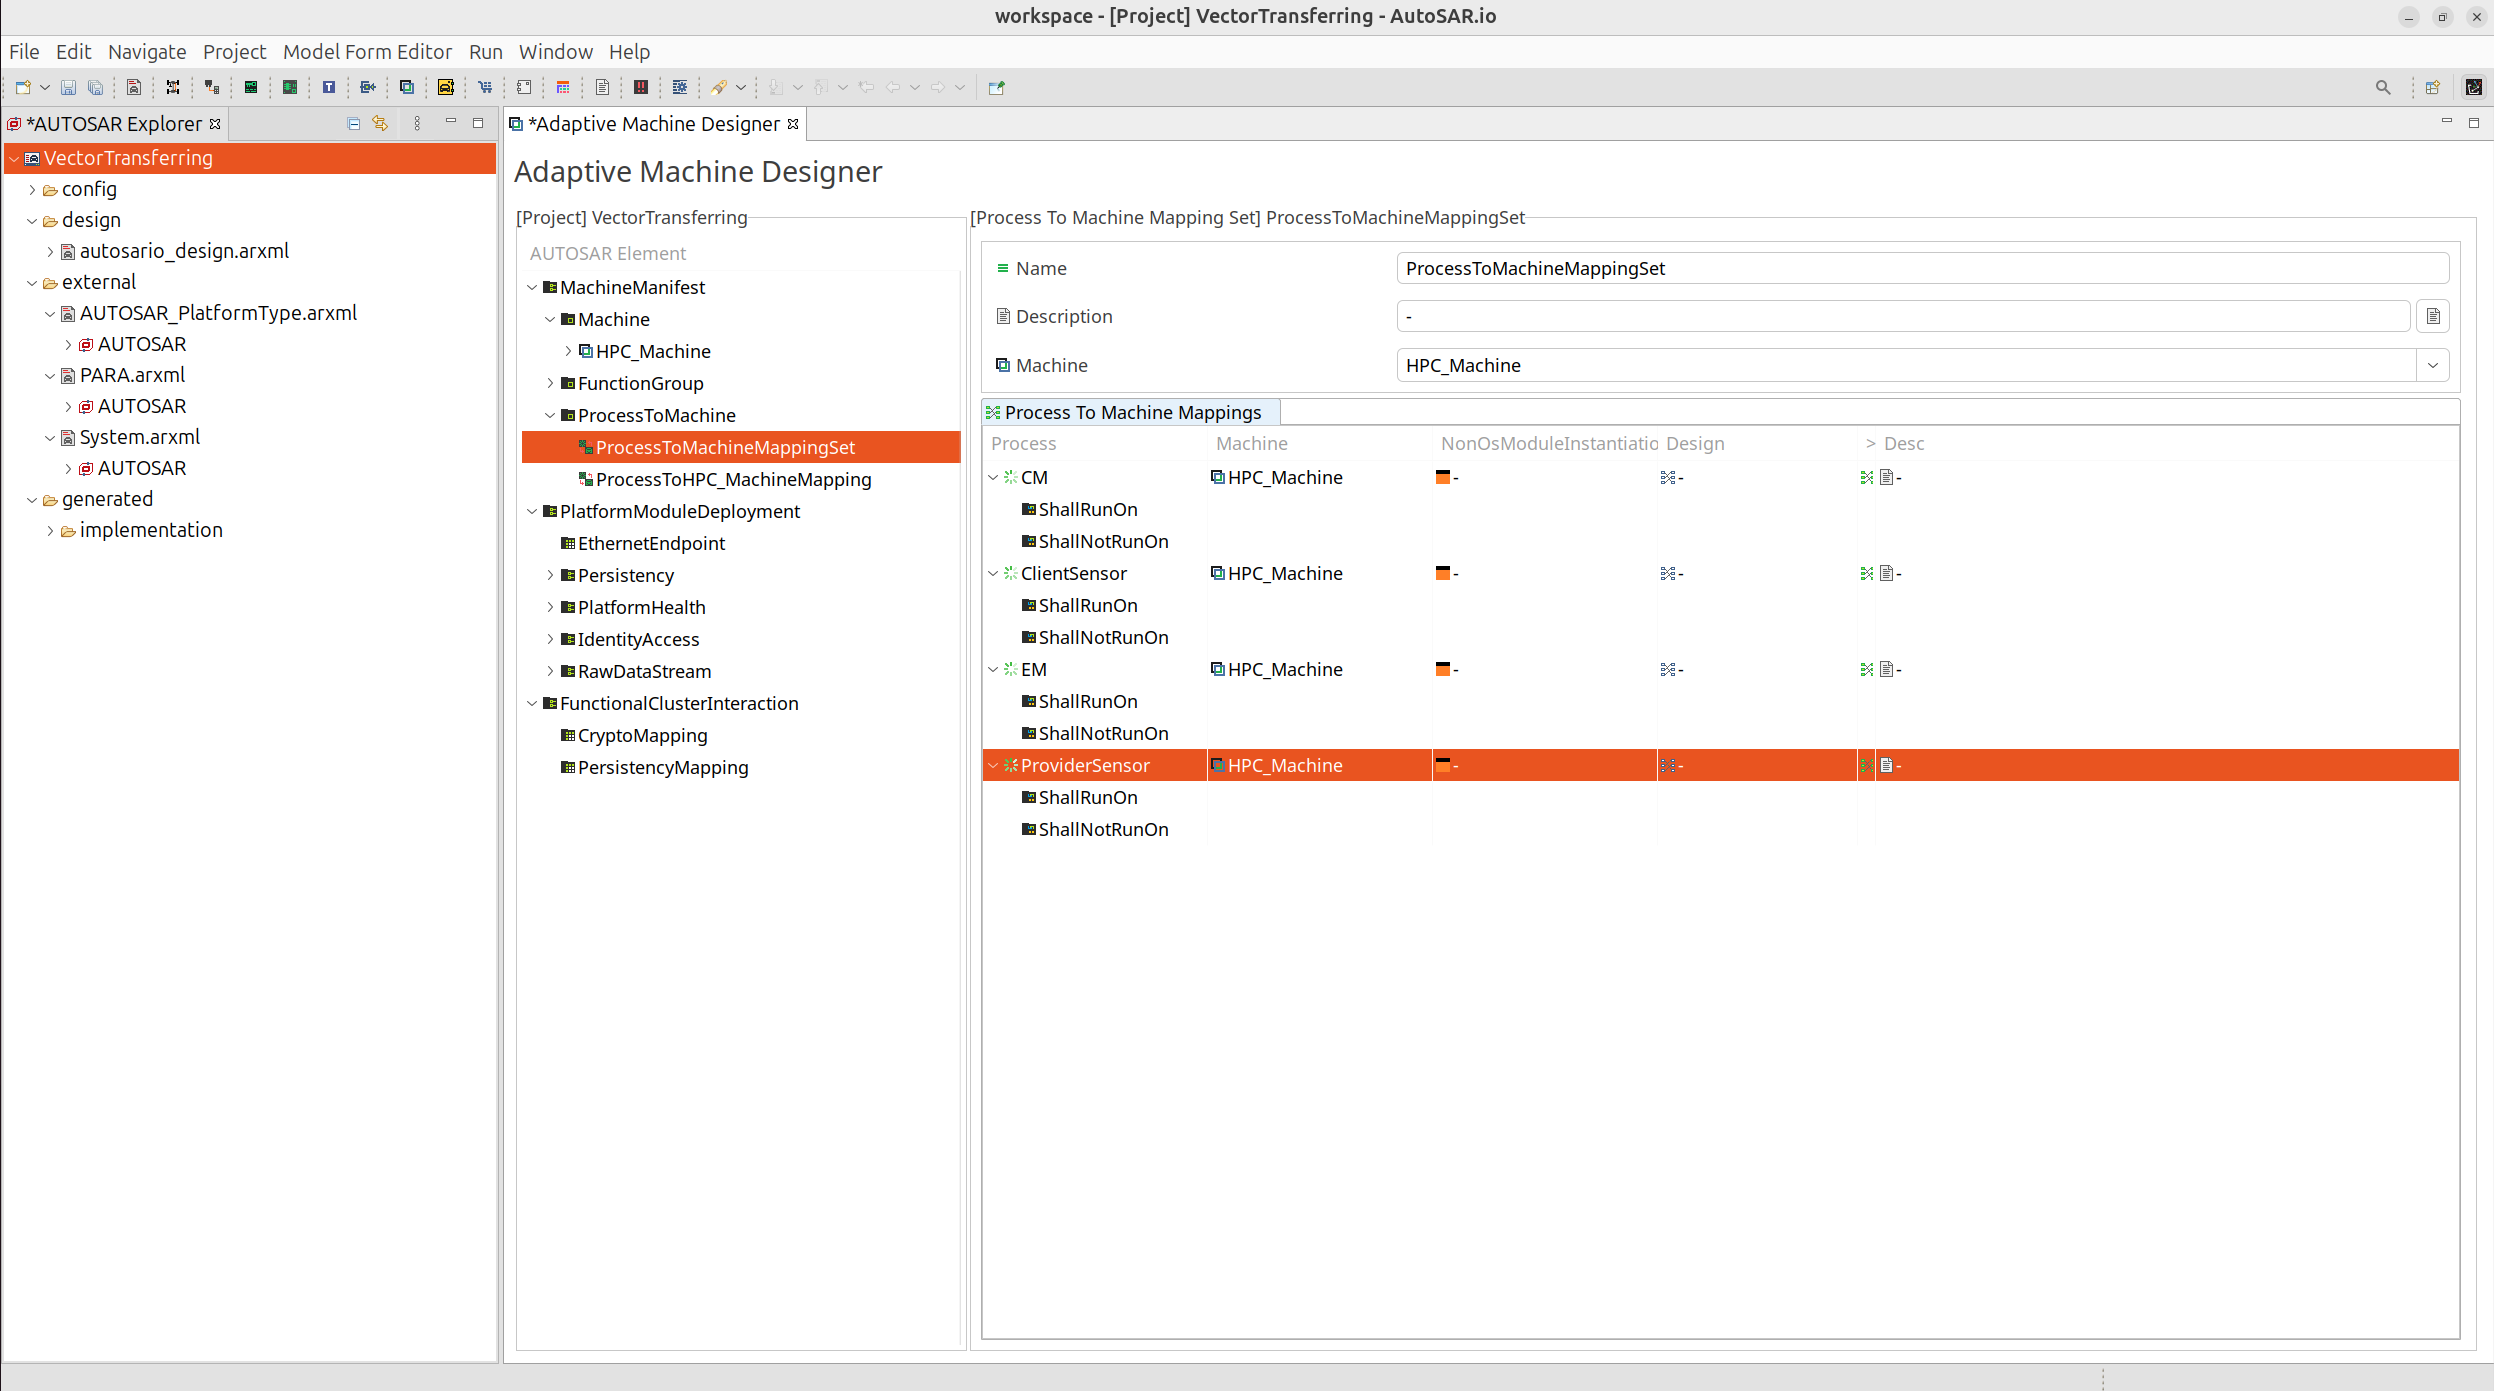
\includegraphics[width=0.75\textwidth]{Images/chap3/image_methodology/applicationDesign/mappingProcesstoMachine.png}
    \vspace{0.5cm}
    \caption{Mapping Application Processes to Target Machine}
    \label{fig:app_process_machine_mapping}
\end{figure}

Finally, Figure~\ref{fig:app_process_machine_mapping} presents the process-to-machine mapping defined in the Adaptive Machine Designer. In this step, all application processes, including \texttt{CM}, \texttt{EM}, \texttt{ClientSensor}, and \texttt{ProviderSensor}, are explicitly assigned to the target \texttt{HPC\_Machine}. This mapping determines the physical execution location of each process and establishes the final deployment relationship between the adaptive applications and the underlying hardware platform.

By consolidating all processes onto a single machine, the configuration ensures a coherent execution environment and simplifies resource management during runtime. This step completes the application deployment workflow by bridging the gap between application-level process definitions and machine-level execution, enabling the Adaptive AUTOSAR runtime to launch and supervise each process according to the previously defined startup, scheduling, and communication configurations.

\subsubsection{Generating Code and Manifest Files}
After completing the configuration steps at the machine, service, and application levels, the Autosar.io tool supports automatic generation of implementation artifacts through the PARA Generator. This generator collects all previously defined models, including Machine Manifests, service definitions, service instances, and application processes, and transforms them into deployable outputs that conform to the Adaptive AUTOSAR specification. By doing so, the tool ensures that the system configuration remains consistent from design time to implementation.

\begin{figure}[H]
    \centering
    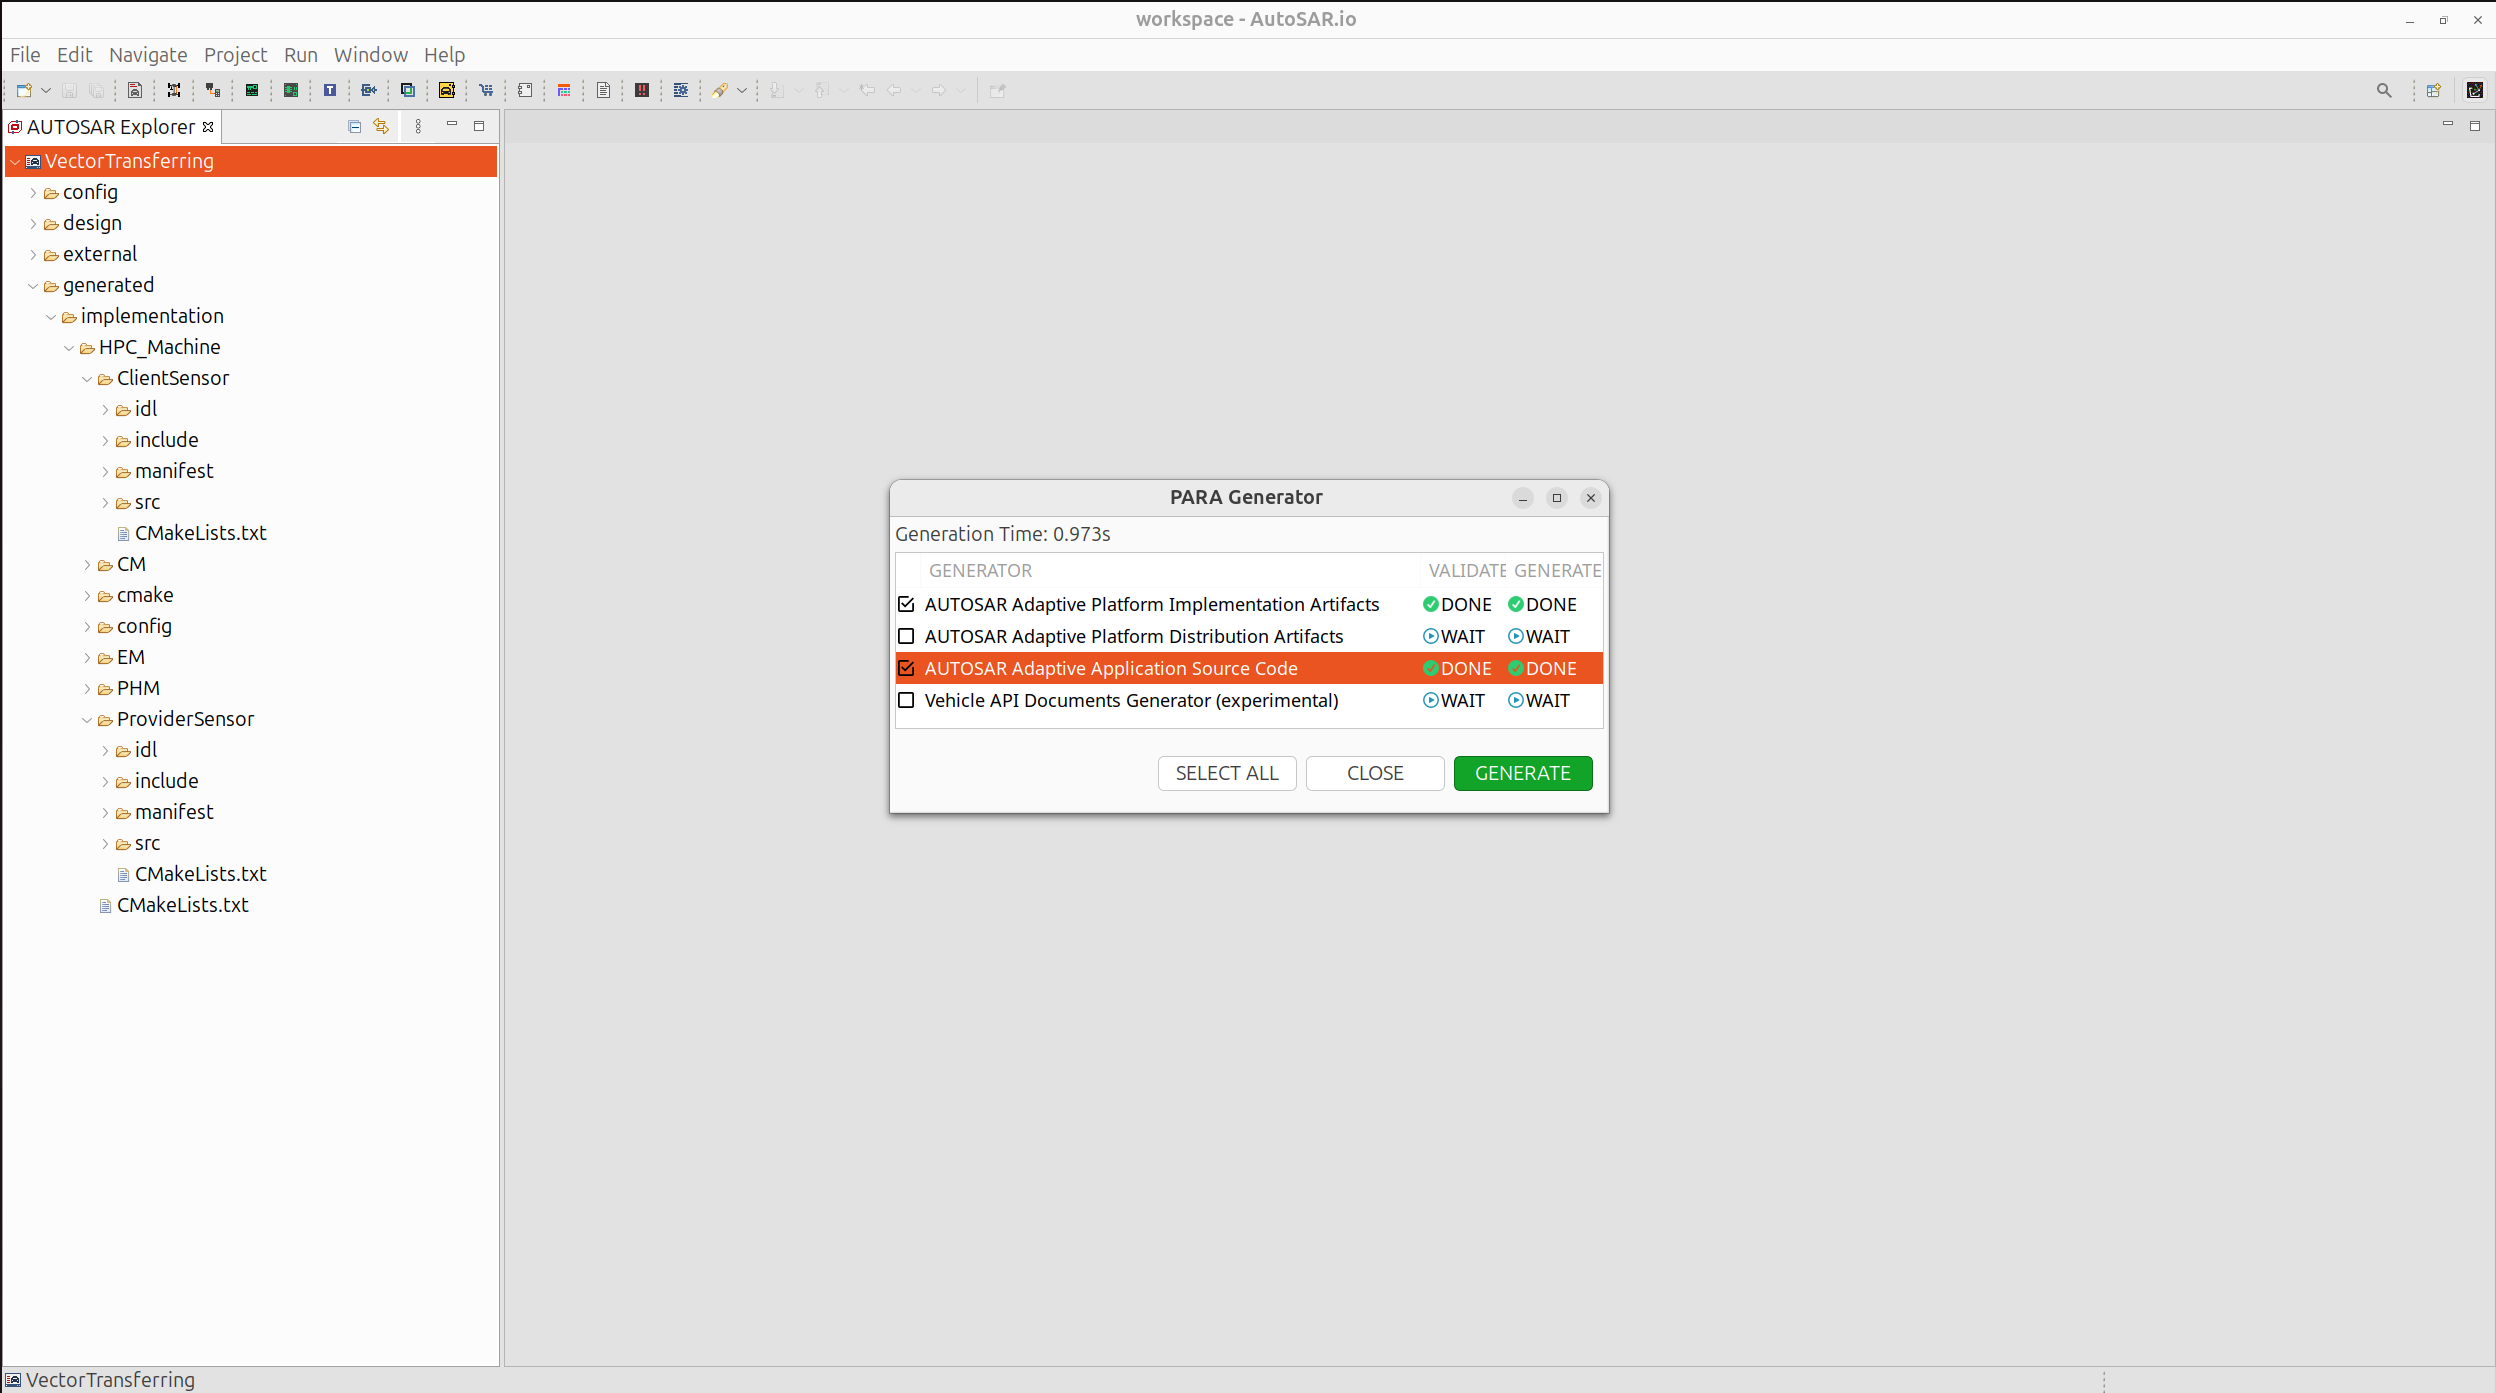
\includegraphics[width=0.75\textwidth]{Images/chap3/generating.png}
    \vspace{0.5cm}
    \caption{Generating Code and ARXML Files}
    \label{fig:code_generation}
\end{figure}

As illustrated in Figure~\ref{fig:code_generation}, the PARA Generator allows users to selectively generate different categories of artifacts, such as Adaptive Application source code, platform configuration files, and manifest descriptions. The generation process produces AUTOSAR compliant ARXML files together with structured C++ source code for each executable. These outputs follow a standardized directory layout, which simplifies subsequent build and integration steps.

Through this automated generation mechanism, Autosar.io bridges the gap between high level system modeling and concrete software artifacts. The generated code and configuration files serve as a reliable foundation for compilation, deployment, and runtime execution. This approach reduces manual errors, improves traceability, and supports a smooth transition from configuration to system integration in the Adaptive AUTOSAR development workflow.


Once the AUTOSAR platform configuration is established, a perception mechanism is required to detect traffic lights in real time. Consequently, the focus shifts to designing and training the YOLO-MobileNetV4 architecture, demonstrating how the core software platform integrates with edge-oriented AI components.

% In this work, we adopt a customized version of the YOLO detection framework by integrating the MobileNetV4 backbone in order to obtain a lightweight yet effective object detection model. The primary motivation behind this design choice is to reduce computational complexity and memory consumption while maintaining reliable detection accuracy. Such requirements are essential for deployment on resource constrained edge devices, including embedded systems, single board computers, and mobile platforms.

% MobileNetV4 is a recently proposed convolutional neural network architecture designed for universal deployment across mobile and edge hardware. It emphasizes efficient feature extraction through improved depthwise separable convolutions, universal inverted bottleneck blocks, and optimized layer scaling strategies. Compared to conventional backbones such as CSPDarknet or standard ResNet variants, MobileNetV4 provides a more balanced trade off between inference speed and representational capability. As a result, it is particularly suitable for real time computer vision tasks where latency, power consumption, and memory footprint are critical constraints.

% \subsection{Backbone Replacement Strategy}

% To integrate MobileNetV4 into the YOLO framework, the default backbone definition is replaced by a customized model configuration file, denoted as \texttt{yolo11-mobilenetv4.yaml}. This configuration follows the standard Ultralytics YOLO model definition format while modifying the backbone section to incorporate MobileNetV4 building blocks. The neck and detection head structures remain largely unchanged in order to preserve compatibility with existing loss functions, anchor settings, and training pipelines.

% The backbone replacement process is performed at the model configuration and module registration level rather than modifying the core training logic. This design choice improves maintainability and simplifies future updates of the YOLO framework. The integration procedure follows a publicly available technical guide that details how MobileNetV4 modules are registered, parsed, and treated as backbone components during model construction\footnote{Guideline for integrating MobileNetV4 into YOLO architectures is available at \url{https://blog.csdn.net/qq_44231797/article/details/147483132}.}. By preserving the feature pyramid structure, multi scale detection capability is maintained despite the lightweight backbone.

% \subsection{Model Initialization and Pretrained Weights}

% To accelerate convergence and improve training stability, the model is initialized using pretrained weights from a lightweight YOLO variant. Specifically, the \texttt{yolo11n.pt} checkpoint is loaded as the initial parameter set. Although the backbone architecture differs from the original YOLO design, partial weight transfer remains beneficial for shared components such as the detection head and certain convolutional layers.

% The Ultralytics YOLO API automatically performs parameter matching where possible and ignores incompatible layers. This mechanism enables the model to leverage prior knowledge while avoiding structural conflicts during initialization. As a result, the training process converges more reliably compared to training from scratch.

% \subsection{Training Configuration}

% The training process is conducted using the Ultralytics YOLO training interface, which provides a flexible and reproducible pipeline for object detection tasks. Dataset information is specified through a YAML configuration file that defines training and validation paths, class labels, and metadata. All input images are resized to a resolution of $320 \times 320$ pixels in order to balance detection accuracy and computational efficiency.

% Stochastic Gradient Descent is selected as the optimization algorithm due to its stable convergence behavior for large scale detection models. Automatic mixed precision is enabled to reduce GPU memory usage and accelerate training while maintaining numerical stability. The model is trained for a total of 400 epochs to ensure sufficient convergence given the modified backbone structure.

% \subsection{Training Script}

% The complete training script used in this study is shown below. This script defines the model configuration, loads pretrained weights, and executes the training process with the selected hyperparameters.

% \begin{lstlisting}[language=Python, caption={YOLO-MobileNetV4 Training Script}]
% # Model configuration file
% model_yaml_path = r"yolo11-mobilenetv4.yaml"

% # Dataset configuration file
% data_yaml_path = r"dataset/data.yaml"

% # Pretrained model
% pre_model_name = "yolo11n.pt"

% import warnings
% warnings.filterwarnings("ignore")

% from ultralytics import YOLO

% if __name__ == "__main__":
%     model = YOLO(model_yaml_path)
%     model.load(pre_model_name)

%     model.train(
%         data=data_yaml_path,
%         cache=False,
%         imgsz=320,
%         epochs=400,
%         workers=8,
%         device="0",
%         optimizer="SGD",
%         amp=True,
%         project="runs/train-yolo-mobilenetv4",
%         name="exp"
%     )
% \end{lstlisting}

\section{YOLO-MobileNetV4 Model}

In this work, we adopt a customized version of the YOLOv26 detection framework by integrating the MobileNetV4 backbone in order to obtain a lightweight yet effective object detection model. The primary motivation behind this design choice is to reduce computational complexity and memory consumption while maintaining reliable detection accuracy. Such requirements are essential for deployment on resource constrained edge devices, including embedded systems, single board computers, and mobile platforms.

\subsection{Integrating MobileNetv4 into YOLO}

Following the our paper in \hyperref[chap:append]{Appendix}, we will continue to integrate MobileNetV4 as the feature extractor for YOLO26 creates a hybrid "YOLO-MNv4" architecture that is theoretically optimal for autonomous driving. On mobile accelerators like the Pixel EdgeTPU, MNv4 is approximately twice as fast as MobileNetV3 for equivalent accuracy due to its high operational intensity. Replacing the standard YOLO26 backbone with MNv4 significantly reduces the floating-point operations (FLOPs) required per inference. This architecture specifically excels in occlusion handling, where the advanced receptive fields of the UIB blocks allow the model to infer the presence of a traffic light even when it is partially obscured by large vehicles, ensuring a robust and reliable perception system.

To adapt the original YOLO26 architecture for edge deployment, several crucial modifications were made (comparing Figure \ref{fig:yolo26_original_arch} to Figure \ref{fig:yolo26_mnv4_arch}). First, the standard heavy CNN backbone was replaced entirely with {MobileNetV4ConvSmall050}. Second, the original 4-head Feature Pyramid Network (P2, P3, P4, P5) was scaled down to a {3-head architecture} (P3, P4, P5) by removing the high-resolution P2 feature extraction path and its corresponding detection head. This reduction dramatically lowers the computational complexity (GFLOPs) and parameter count. Meanwhile, the advanced components of the YOLO26 neck—including the {C3k2} fusion blocks, {SPPF}, {C2PSA} spatial attention, and the {One-to-One Head}-were preserved to maintain state-of-the-art detection logic.

\begin{figure}[htbp]
    \centering
    \resizebox{\textwidth}{!}{
    \begin{tikzpicture}[
        box/.style={rectangle, draw, minimum width=2.4cm, minimum height=0.8cm, text centered, font=\sffamily, rounded corners=2pt},
        arrow/.style={->, >=stealth, thick},
        label/.style={font=\sffamily\scriptsize}
    ]

    % Backbone
    \node[box, fill=blue!10] (input) at (0, 9) {Input (640)};
    \node[box, fill=green!10] (conv1) at (0, 7.5) {Conv P1};
    \node[box, fill=green!10] (p2) at (0, 6) {P2 (C3k2)};
    \node[box, fill=green!10] (p3) at (0, 4) {P3 (C3k2)};
    \node[box, fill=green!10] (p4) at (0, 2) {P4 (C3k2)};
    \node[box, fill=green!10] (p5) at (0, 0) {P5 (C2PSA)};

    \draw[arrow] (input) -- (conv1);
    \draw[arrow] (conv1) -- (p2);
    \draw[arrow] (p2) -- (p3);
    \draw[arrow] (p3) -- (p4);
    \draw[arrow] (p4) -- (p5);

    % SPPF & C2PSA
    \node[box, fill=yellow!10] (sppf) at (3.5, 0) {SPPF};
    \node[box, fill=yellow!10] (c2psa) at (7.0, 0) {C2PSA};
    \draw[arrow] (p5) -- (sppf);
    \draw[arrow] (sppf) -- (c2psa);

    % Neck - Top-down
    \node[box, fill=orange!10] (cat_p4) at (7.0, 2) {Concat};
    \node[box, fill=orange!10] (c3k2_td_p4) at (10.5, 2) {C3k2};
    \draw[arrow] (c2psa) -- node[right, label] {Up} (cat_p4);
    \draw[arrow] (p4) -- (cat_p4);
    \draw[arrow] (cat_p4) -- (c3k2_td_p4);

    \node[box, fill=orange!10] (cat_p3) at (10.5, 4) {Concat};
    \node[box, fill=orange!10] (c3k2_td_p3) at (14.0, 4) {C3k2};
    \draw[arrow] (c3k2_td_p4) -- node[right, label] {Up} (cat_p3);
    \draw[arrow] (p3) -- (cat_p3);
    \draw[arrow] (cat_p3) -- (c3k2_td_p3);

    \node[box, fill=orange!10] (cat_p2) at (14.0, 6) {Concat};
    \node[box, fill=orange!10] (c3k2_td_p2) at (17.5, 6) {C3k2};
    \draw[arrow] (c3k2_td_p3) -- node[right, label] {Up} (cat_p2);
    \draw[arrow] (p2) -- (cat_p2);
    \draw[arrow] (cat_p2) -- (c3k2_td_p2);

    % Neck - Bottom-up
    \node[box, fill=orange!10] (cat_p3_bu) at (17.5, 4) {Concat};
    \node[box, fill=orange!10] (c3k2_bu_p3) at (21.0, 4) {C3k2};
    \draw[arrow] (c3k2_td_p2) -- node[right, label] {Conv s2} (cat_p3_bu);
    \draw[arrow] (c3k2_td_p3) -- (cat_p3_bu);
    \draw[arrow] (cat_p3_bu) -- (c3k2_bu_p3);

    \node[box, fill=orange!10] (cat_p4_bu) at (21.0, 2) {Concat};
    \node[box, fill=orange!10] (c3k2_bu_p4) at (24.5, 2) {C3k2};
    \draw[arrow] (c3k2_bu_p3) -- node[right, label] {Conv s2} (cat_p4_bu);
    \draw[arrow] (c3k2_td_p4) -- (cat_p4_bu);
    \draw[arrow] (cat_p4_bu) -- (c3k2_bu_p4);

    \node[box, fill=orange!10] (cat_p5_bu) at (24.5, 0) {Concat};
    \node[box, fill=orange!10] (c3k2_bu_p5) at (28.0, 0) {C3k2};
    \draw[arrow] (c3k2_bu_p4) -- node[right, label] {Conv s2} (cat_p5_bu);
    \draw[arrow] (c2psa) -- (cat_p5_bu);
    \draw[arrow] (cat_p5_bu) -- (c3k2_bu_p5);

    % Detectors
    \node[box, fill=red!10] (head2) at (31.5, 6) {Detect P2};
    \node[box, fill=red!10] (head3) at (31.5, 4) {Detect P3};
    \node[box, fill=red!10] (head4) at (31.5, 2) {Detect P4};
    \node[box, fill=red!10] (head5) at (31.5, 0) {Detect P5};
    
    \node[box, fill=purple!10, align=center, minimum height=1.6cm] (detect) at (35.0, 3) {One-to-One\\Head};

    \draw[arrow] (c3k2_td_p2) -- (head2);
    \draw[arrow] (c3k2_bu_p3) -- (head3);
    \draw[arrow] (c3k2_bu_p4) -- (head4);
    \draw[arrow] (c3k2_bu_p5) -- (head5);
    
    \draw[arrow] (head2) -| (detect);
    \draw[arrow] (head3) -| (detect);
    \draw[arrow] (head4) -| (detect);
    \draw[arrow] (head5) -| (detect);

    \end{tikzpicture}
    }
    \vspace{0.5cm}
    \caption{Architecture of the original YOLO26-p2 model with 4-head detection mechanism (P2/P3/P4/P5 outputs) for standard object detection tasks. Channel widths scale with the chosen model variant (n/s/m/l/x).}
    \label{fig:yolo26_original_arch}
\end{figure}

\begin{figure}[htbp]
    \centering
    \resizebox{\textwidth}{!}{
    \begin{tikzpicture}[
        box/.style={rectangle, draw, minimum width=2.4cm, minimum height=0.8cm, text centered, font=\sffamily, rounded corners=2pt},
        arrow/.style={->, >=stealth, thick},
        label/.style={font=\sffamily\scriptsize}
    ]

    % X coordinates:
    % 0.0: Backbone
    % 3.5: SPPF
    % 7.0: C2PSA, cat1
    % 10.5: c3k2_1, cat2
    % 14.0: c3k2_2, cat3
    % 17.5: c3k2_3, cat4
    % 21.0: c3k2_4
    % 24.5: Detectors
    % 28.0: Head

    % Backbone
    \node[box, fill=blue!10] (input) at (0, 8) {Input (416)};
    \node[box, fill=green!10] (mnv4) at (0, 6) {MobileNetV4};
    \node[box, fill=green!10] (p3) at (0, 4) {P3 (32c)};
    \node[box, fill=green!10] (p4) at (0, 2) {P4 (48c)};
    \node[box, fill=green!10] (p5) at (0, 0) {P5 (640c)};

    \draw[arrow] (input) -- (mnv4);
    \draw[arrow] (mnv4) -- (p3);
    \draw[arrow] (p3) -- (p4);
    \draw[arrow] (p4) -- (p5);

    % SPPF & C2PSA
    \node[box, fill=yellow!10] (sppf) at (3.5, 0) {SPPF (256c)};
    \node[box, fill=yellow!10] (c2psa) at (7.0, 0) {C2PSA (256c)};
    \draw[arrow] (p5) -- (sppf);
    \draw[arrow] (sppf) -- (c2psa);

    % Neck - Top-down
    \node[box, fill=orange!10] (cat1) at (7.0, 2) {Concat};
    \node[box, fill=orange!10] (c3k2_1) at (10.5, 2) {C3k2 (128c)};
    \draw[arrow] (c2psa) -- node[right, label] {Up} (cat1);
    \draw[arrow] (p4) -- (cat1);
    \draw[arrow] (cat1) -- (c3k2_1);

    \node[box, fill=orange!10] (cat2) at (10.5, 4) {Concat};
    \node[box, fill=orange!10] (c3k2_2) at (14.0, 4) {C3k2 (64c)};
    \draw[arrow] (c3k2_1) -- node[right, label] {Up} (cat2);
    \draw[arrow] (p3) -- (cat2);
    \draw[arrow] (cat2) -- (c3k2_2);

    % Neck - Bottom-up
    \node[box, fill=orange!10] (cat3) at (14.0, 2) {Concat};
    \node[box, fill=orange!10] (c3k2_3) at (17.5, 2) {C3k2 (128c)};
    \draw[arrow] (c3k2_2) -- node[right, label] {Conv s2} (cat3);
    \draw[arrow] (c3k2_1) -- (cat3);
    \draw[arrow] (cat3) -- (c3k2_3);

    \node[box, fill=orange!10] (cat4) at (17.5, 0) {Concat};
    \node[box, fill=orange!10] (c3k2_4) at (21.0, 0) {C3k2 (256c)};
    \draw[arrow] (c3k2_3) -- node[right, label] {Conv s2} (cat4);
    \draw[arrow] (c2psa) -- (cat4);
    \draw[arrow] (cat4) -- (c3k2_4);

    % Detectors
    \node[box, fill=red!10] (head1) at (24.5, 4) {Detect P3};
    \node[box, fill=red!10] (head2) at (24.5, 2) {Detect P4};
    \node[box, fill=red!10] (head3) at (24.5, 0) {Detect P5};
    
    \node[box, fill=purple!10, align=center] (detect) at (28.0, 2) {One-to-One\\Head};

    \draw[arrow] (c3k2_2) -- (head1);
    \draw[arrow] (c3k2_3) -- (head2);
    \draw[arrow] (c3k2_4) -- (head3);
    
    \draw[arrow] (head1) -| (detect);
    \draw[arrow] (head2) -- (detect);
    \draw[arrow] (head3) -| (detect);

    \end{tikzpicture}
    }
    \vspace{0.5cm} % Add some space before caption to prevent overlap
    \caption{Architecture of the YOLO26 model with MobileNetV4ConvSmall050 backbone, dual-head mechanism, and NMS-free end-to-end detection, tailored for $416\times416$ resolution.}
    \label{fig:yolo26_mnv4_arch}
\end{figure}

% \subsection{Training Hyperparameters}

% The training process is conducted using the Ultralytics YOLO training API, which provides a reproducible and configurable pipeline for object detection tasks. The dataset is specified through a YAML configuration file (\texttt{TrafficLightV5.v9i.yolo26/data.yaml}) that defines training and validation image paths, class labels, and metadata. To bootstrap training, pretrained weights from \texttt{yolo26n.pt} are loaded via partial weight transfer; compatible layers (primarily in the neck and head) inherit learned parameters, while the MobileNetV4 backbone is initialised from scratch. The \texttt{end2end=True} flag activates the One-to-One head for NMS-free training. Table~\ref{tab:hyperparams} summarises the key hyperparameters.

% \begin{table}[htbp]
% \centering
% \caption{Selected training hyperparameters for the YOLO26-MobileNetV4 model.}
% \label{tab:hyperparams}
% \renewcommand{\arraystretch}{1.15}
% \begin{tabular}{l l l}
% \hline
% \textbf{Parameter} & \textbf{Value} & \textbf{Rationale} \\
% \hline
% \texttt{imgsz} & $416 \times 416$ & Balance between spatial resolution and edge inference speed \\
% \texttt{epochs} & 100 & Sufficient convergence for the modified backbone \\
% \texttt{batch} & 16 & Fits within GPU memory with MobileNetV4 backbone \\
% \texttt{patience} & 100 & Disable early stopping; run full cosine LR cycle \\
% \texttt{optimizer} & auto (SGD) & Stable convergence for detection models \\
% \texttt{lr0} & 0.005 & Slightly elevated initial LR for unfrozen backbone \\
% \texttt{lrf} & 0.01 & Final LR ratio: $\text{lr}_{\text{final}} = 0.01 \times \text{lr}_0$ \\
% \texttt{cos\_lr} & True & Cosine annealing for smooth convergence in late epochs \\
% \texttt{warmup\_epochs} & 3.0 & Gradual LR ramp-up to stabilise early gradients \\
% \texttt{amp} & True & Mixed-precision training for memory efficiency \\
% \texttt{freeze} & None & All layers trainable; no backbone freezing \\
% \texttt{close\_mosaic} & 10 & Disable mosaic augmentation in the last 10 epochs \\
% \hline
% \texttt{box} & 7.5 & Bounding box regression loss weight \\
% \texttt{cls} & 0.5 & Classification loss weight \\
% \texttt{dfl} & 1.5 & DFL loss weight (set but unused since YOLO26 removes DFL) \\
% \hline
% \end{tabular}
% \end{table}

% \subsubsection{Optimiser and Learning Rate Schedule}
% The optimiser is set to \texttt{auto}, which defaults to Stochastic Gradient Descent (SGD) with Nesterov momentum ($\mu = 0.937$) and weight decay ($\lambda = 5 \times 10^{-4}$). The initial learning rate is set to $\text{lr}_0 = 0.005$, slightly higher than the default $0.01$ to compensate for the unfrozen MobileNetV4 backbone requiring larger gradient steps to adapt to the traffic light domain. A cosine annealing schedule (\texttt{cos\_lr=True}) smoothly decays the learning rate to $\text{lr}_0 \times \text{lrf} = 5 \times 10^{-5}$ over the full 100 epochs, ensuring fine-grained convergence in the later stages of training without the abrupt transitions of step-decay schedules.

% \subsubsection{No Backbone Freezing}
% Unlike transfer learning approaches that freeze the backbone during initial epochs, this configuration leaves all layers trainable (\texttt{freeze=None}). Since the MobileNetV4ConvSmall050 backbone differs fundamentally from the original YOLO26 backbone, the pretrained weights only partially transfer. Freezing would prevent the new backbone from learning domain-specific features such as the distinctive shapes and colours of Vietnamese traffic light signal heads and arrow indicators.

% \subsubsection{Image Augmentation Strategy}
% The augmentation pipeline is carefully tuned for the traffic light detection domain:

% \begin{itemize}
%     \item \textbf{Colour jitter}: Hue shift is minimal (\texttt{hsv\_h}$=0.015$) to preserve the critical red/green/yellow colour semantics of traffic signals. Saturation (\texttt{hsv\_s}$=0.7$) and brightness (\texttt{hsv\_v}$=0.4$) augmentation are moderate to improve robustness under varying lighting conditions without corrupting colour-dependent class distinctions.
%     \item \textbf{Geometric transforms}: Translation (\texttt{translate}$=0.1$) and scale (\texttt{scale}$=0.5$) are enabled to simulate varying camera distances and positions. Rotation (\texttt{degrees}$=0.0$) and shear (\texttt{shear}$=0.0$) are disabled since traffic lights are always vertically oriented.
%     \item \textbf{Flipping disabled}: Both horizontal (\texttt{fliplr}$=0.0$) and vertical (\texttt{flipud}$=0.0$) flips are strictly disabled. Horizontal flipping would reverse the direction of left/right arrow turn signals, creating incorrect training labels.
%     \item \textbf{Mosaic}: Set to 0.5 probability to composite multiple training images into one frame, improving the model's ability to detect small, densely packed objects such as timer digit clusters. Mosaic is automatically disabled in the last 10 epochs (\texttt{close\_mosaic}$=10$) so the model fine-tunes on unmodified real images.
%     \item \textbf{MixUp and CopyPaste}: Both disabled (\texttt{mixup}$=0.0$, \texttt{copy\_paste}$=0.0$) to avoid blending signals from different classes, which could confuse the network on colour-critical traffic light states.
% \end{itemize}


\subsection{Dataset and Hyper parameters}
\label{sub:datasetYolo}
A well-prepared dataset and carefully tuned hyperparameters are essential for successfully training the modified YOLO-MobileNetV4 model. This section details the dataset used for traffic light detection, including its composition and pre-processing steps, before explaining the specific training configurations and augmentation strategies applied to ensure robust performance.

\subsubsection{Dataset Composition and Pre-processing}
The model is trained and evaluated on the \texttt{TrafficLightV5.v9i.yolo26} dataset, which comprises a total of 4,867 images. The dataset is annotated in the YOLO format and structured to detect four classes: \texttt{left}, \texttt{right}, \texttt{straight}, and \texttt{timer}. The images are partitioned into three splits: 4,260 images for training, 406 for validation, and 201 for testing. Prior to model ingestion, offline pre-processing and augmentations were applied via Roboflow. The pre-processing includes auto-orientation and resizing to $416 \times 416$ pixels (fit with black edges). The offline augmentation strategy generates three versions of each source image by applying random rotation ($-5^\circ$ to $+5^\circ$), random shear ($-2^\circ$ to $+2^\circ$), exposure adjustments ($\pm 10\%$), and salt-and-pepper noise ($0.1\%$ of pixels).

\subsubsection{Training Configuration}
The training process is conducted using the Ultralytics YOLO training API, which provides a reproducible and configurable pipeline for object detection tasks. The dataset is specified through a YAML configuration file (\texttt{TrafficLightV5.v9i.yolo26/data.yaml}) that defines training and validation image paths, class labels, and metadata. To bootstrap training, pretrained weights from \texttt{yolo26n.pt} are loaded via partial weight transfer; compatible layers (primarily in the neck and head) inherit learned parameters, while the MobileNetV4 backbone is initialised from scratch. The \texttt{end2end=True} flag activates the One-to-One head for NMS-free training. Table~\ref{tab:hyperparams} summarises the key hyperparameters.

\begin{table}[htbp]
\centering
\caption{Selected training hyperparameters for the YOLO26-MobileNetV4 model.}
\label{tab:hyperparams}
\renewcommand{\arraystretch}{1.15}
\begin{tabular}{l l l}
\hline
\textbf{Parameter} & \textbf{Value} & \textbf{Rationale} \\
\hline
\texttt{imgsz} & $416 \times 416$ & Balance between spatial resolution and edge inference speed \\
\texttt{epochs} & 100 & Sufficient convergence for the modified backbone \\
\texttt{batch} & 16 & Fits within GPU memory with MobileNetV4 backbone \\
\texttt{patience} & 100 & Disable early stopping; run full cosine LR cycle \\
\texttt{optimizer} & auto (SGD) & Stable convergence for detection models \\
\texttt{lr0} & 0.005 & Slightly elevated initial LR for unfrozen backbone \\
\texttt{lrf} & 0.01 & Final LR ratio: $\text{lr}_{\text{final}} = 0.01 \times \text{lr}_0$ \\
\texttt{cos\_lr} & True & Cosine annealing for smooth convergence in late epochs \\
\texttt{warmup\_epochs} & 3.0 & Gradual LR ramp-up to stabilise early gradients \\
\texttt{amp} & True & Mixed-precision training for memory efficiency \\
\texttt{freeze} & None & All layers trainable; no backbone freezing \\
\texttt{close\_mosaic} & 10 & Disable mosaic augmentation in the last 10 epochs \\
\hline
\texttt{box} & 7.5 & Bounding box regression loss weight \\
\texttt{cls} & 0.5 & Classification loss weight \\
\texttt{dfl} & 1.5 & DFL loss weight (set but unused since YOLO26 removes DFL) \\
\hline
\end{tabular}
\end{table}

\subsubsection{Optimiser and Learning Rate Schedule}
The optimiser is set to \texttt{auto}, which defaults to Stochastic Gradient Descent (SGD) with Nesterov momentum ($\mu = 0.937$) and weight decay ($\lambda = 5 \times 10^{-4}$). The initial learning rate is set to $\text{lr}_0 = 0.005$, slightly higher than the default $0.01$ to compensate for the unfrozen MobileNetV4 backbone requiring larger gradient steps to adapt to the traffic light domain. A cosine annealing schedule (\texttt{cos\_lr=True}) smoothly decays the learning rate to $\text{lr}_0 \times \text{lrf} = 5 \times 10^{-5}$ over the full 100 epochs, ensuring fine-grained convergence in the later stages of training without the abrupt transitions of step-decay schedules.

\subsubsection{No Backbone Freezing}
Unlike transfer learning approaches that freeze the backbone during initial epochs, this configuration leaves all layers trainable (\texttt{freeze=None}). Since the MobileNetV4ConvSmall050 backbone differs fundamentally from the original YOLO26 backbone, the pretrained weights only partially transfer. Freezing would prevent the new backbone from learning domain-specific features such as the distinctive shapes and colours of Vietnamese traffic light signal heads and arrow indicators.

\subsubsection{Image Augmentation Strategy}
The augmentation pipeline is carefully tuned for the traffic light detection domain:

\begin{itemize}
    \item \textbf{Colour jitter}: Hue shift is minimal (\texttt{hsv\_h}$=0.015$) to preserve the critical red/green/yellow colour semantics of traffic signals. Saturation (\texttt{hsv\_s}$=0.7$) and brightness (\texttt{hsv\_v}$=0.4$) augmentation are moderate to improve robustness under varying lighting conditions without corrupting colour-dependent class distinctions.
    \item \textbf{Geometric transforms}: Translation (\texttt{translate}$=0.1$) and scale (\texttt{scale}$=0.5$) are enabled to simulate varying camera distances and positions. Rotation (\texttt{degrees}$=0.0$) and shear (\texttt{shear}$=0.0$) are disabled since traffic lights are always vertically oriented.
    \item \textbf{Flipping disabled}: Both horizontal (\texttt{fliplr}$=0.0$) and vertical (\texttt{flipud}$=0.0$) flips are strictly disabled. Horizontal flipping would reverse the direction of left/right arrow turn signals, creating incorrect training labels.
    \item \textbf{Mosaic}: Set to 0.5 probability to composite multiple training images into one frame, improving the model's ability to detect small, densely packed objects such as timer digit clusters. Mosaic is automatically disabled in the last 10 epochs (\texttt{close\_mosaic}$=10$) so the model fine-tunes on unmodified real images.
    \item \textbf{MixUp and CopyPaste}: Both disabled (\texttt{mixup}$=0.0$, \texttt{copy\_paste}$=0.0$) to avoid blending signals from different classes, which could confuse the network on colour-critical traffic light states.
\end{itemize}

\subsection{Exporting to TFLite with INT8 Quantisation}

To deploy the trained YOLO26-MobileNetV4 model on edge devices such as the Raspberry Pi 5, the model must be converted from its native PyTorch format to TensorFlow Lite (TFLite). The Ultralytics export pipeline automates this multi-stage conversion: PyTorch $\to$ ONNX $\to$ TensorFlow SavedModel $\to$ TFLite. The export is performed with the following configuration:

\begin{lstlisting}[language=Python, caption={YOLO26-MobileNetV4 TFLite export script.}, label={lst:export}]
from ultralytics import YOLO

model = YOLO("runs/train/yolo26_mobilenetv4_custom/weights/best.pt")

model.export(
    format="tflite",
    imgsz=416,
    int8=True,
    data='TrafficLightV5.v9i.yolo26/data.yaml',
    batch=1,
    end2end=True,
)
\end{lstlisting}

\subsubsection{INT8 Post-Training Quantisation.}
Full-integer quantisation maps all floating-point weights and activations to 8-bit integers, reducing the model size by approximately $4\times$ and enabling the use of integer-only arithmetic on ARM NEON SIMD units. The quantisation scheme represents each tensor value $x$ as:

\begin{equation}
\label{eq:quant}
  x_q = \text{round}\!\left(\frac{x}{s}\right) + z,
  \qquad
  s = \frac{x_{\max} - x_{\min}}{255},
  \qquad
  z = \text{round}\!\left(-\frac{x_{\min}}{s}\right),
\end{equation}

where $s$ is the per-tensor scale factor and $z$ is the zero-point, both determined during the calibration phase. To compute these statistics, a representative subset of training images from the dataset specified by the \texttt{data} parameter is fed through the network. This calibration step records the dynamic range of each activation tensor, enabling the converter to choose optimal scale and zero-point values that minimise quantisation error across the domain-specific input distribution.

\subsubsection{End-to-End Export}
The \texttt{end2end=True} flag preserves the One-to-One detection head in the exported model graph, ensuring that the TFLite model produces final detection results directly without requiring an external NMS post-processing step. This is critical for edge deployment because it eliminates the need for custom NMS operators that may not be supported by all TFLite delegates, and guarantees deterministic output tensor shapes $(1, 300, 6)$ regardless of input content.

\subsubsection{Deployment Considerations}
The resulting INT8 TFLite model is deployed via the LiteRT (formerly TensorFlow Lite) interpreter on the target device. With \texttt{batch=1} and \texttt{imgsz=416}, the model is optimised for single-frame, real-time inference. The quantised flatbuffer file is significantly smaller than the original float32 model, fitting within the L2 cache of the Cortex-A76 cores on the Raspberry Pi 5, which minimises memory access latency during inference.

% \subsubsection{Accuracy}

% Based on the quantitative trends observed in Figures~\ref{fig:yolomobilenetv4} and~\ref{fig:code_generation}, the original YOLOv11n model achieves slightly higher detection accuracy compared to the YOLOv11n-MobileNetV4 variant. Specifically, the original model attains marginally better precision, recall, and mean Average Precision across the evaluated metrics.

% From the mAP@50 curves, the original YOLOv11n model achieves an improvement of approximately 10--15\% compared to the MobileNetV4-based model. A similar performance gap is observed for mAP@50--95, where the original architecture demonstrates around 10--15\% higher accuracy under stricter localization thresholds. These differences indicate that the original backbone provides stronger feature representation capability, particularly for precise object localization.

% Nevertheless, the overall performance gap remains relatively small. The YOLO-MobileNetV4 model preserves more than 95\% of the detection accuracy achieved by the original YOLOv11n while significantly reducing model complexity. Precision and recall curves further confirm that both models exhibit comparable convergence behavior, with the MobileNetV4 variant showing slightly lower but stable accuracy throughout training.

% These results highlight a clear trade off between accuracy and efficiency. While the original YOLOv11n model offers slightly superior detection accuracy, the YOLO-MobileNetV4 configuration provides a more balanced solution by achieving competitive accuracy with reduced computational cost. This balance makes the MobileNetV4-based model particularly suitable for deployment in edge oriented and resource constrained environments where efficiency is a primary concern.


% \begin{figure}[H]
%     \centering
%     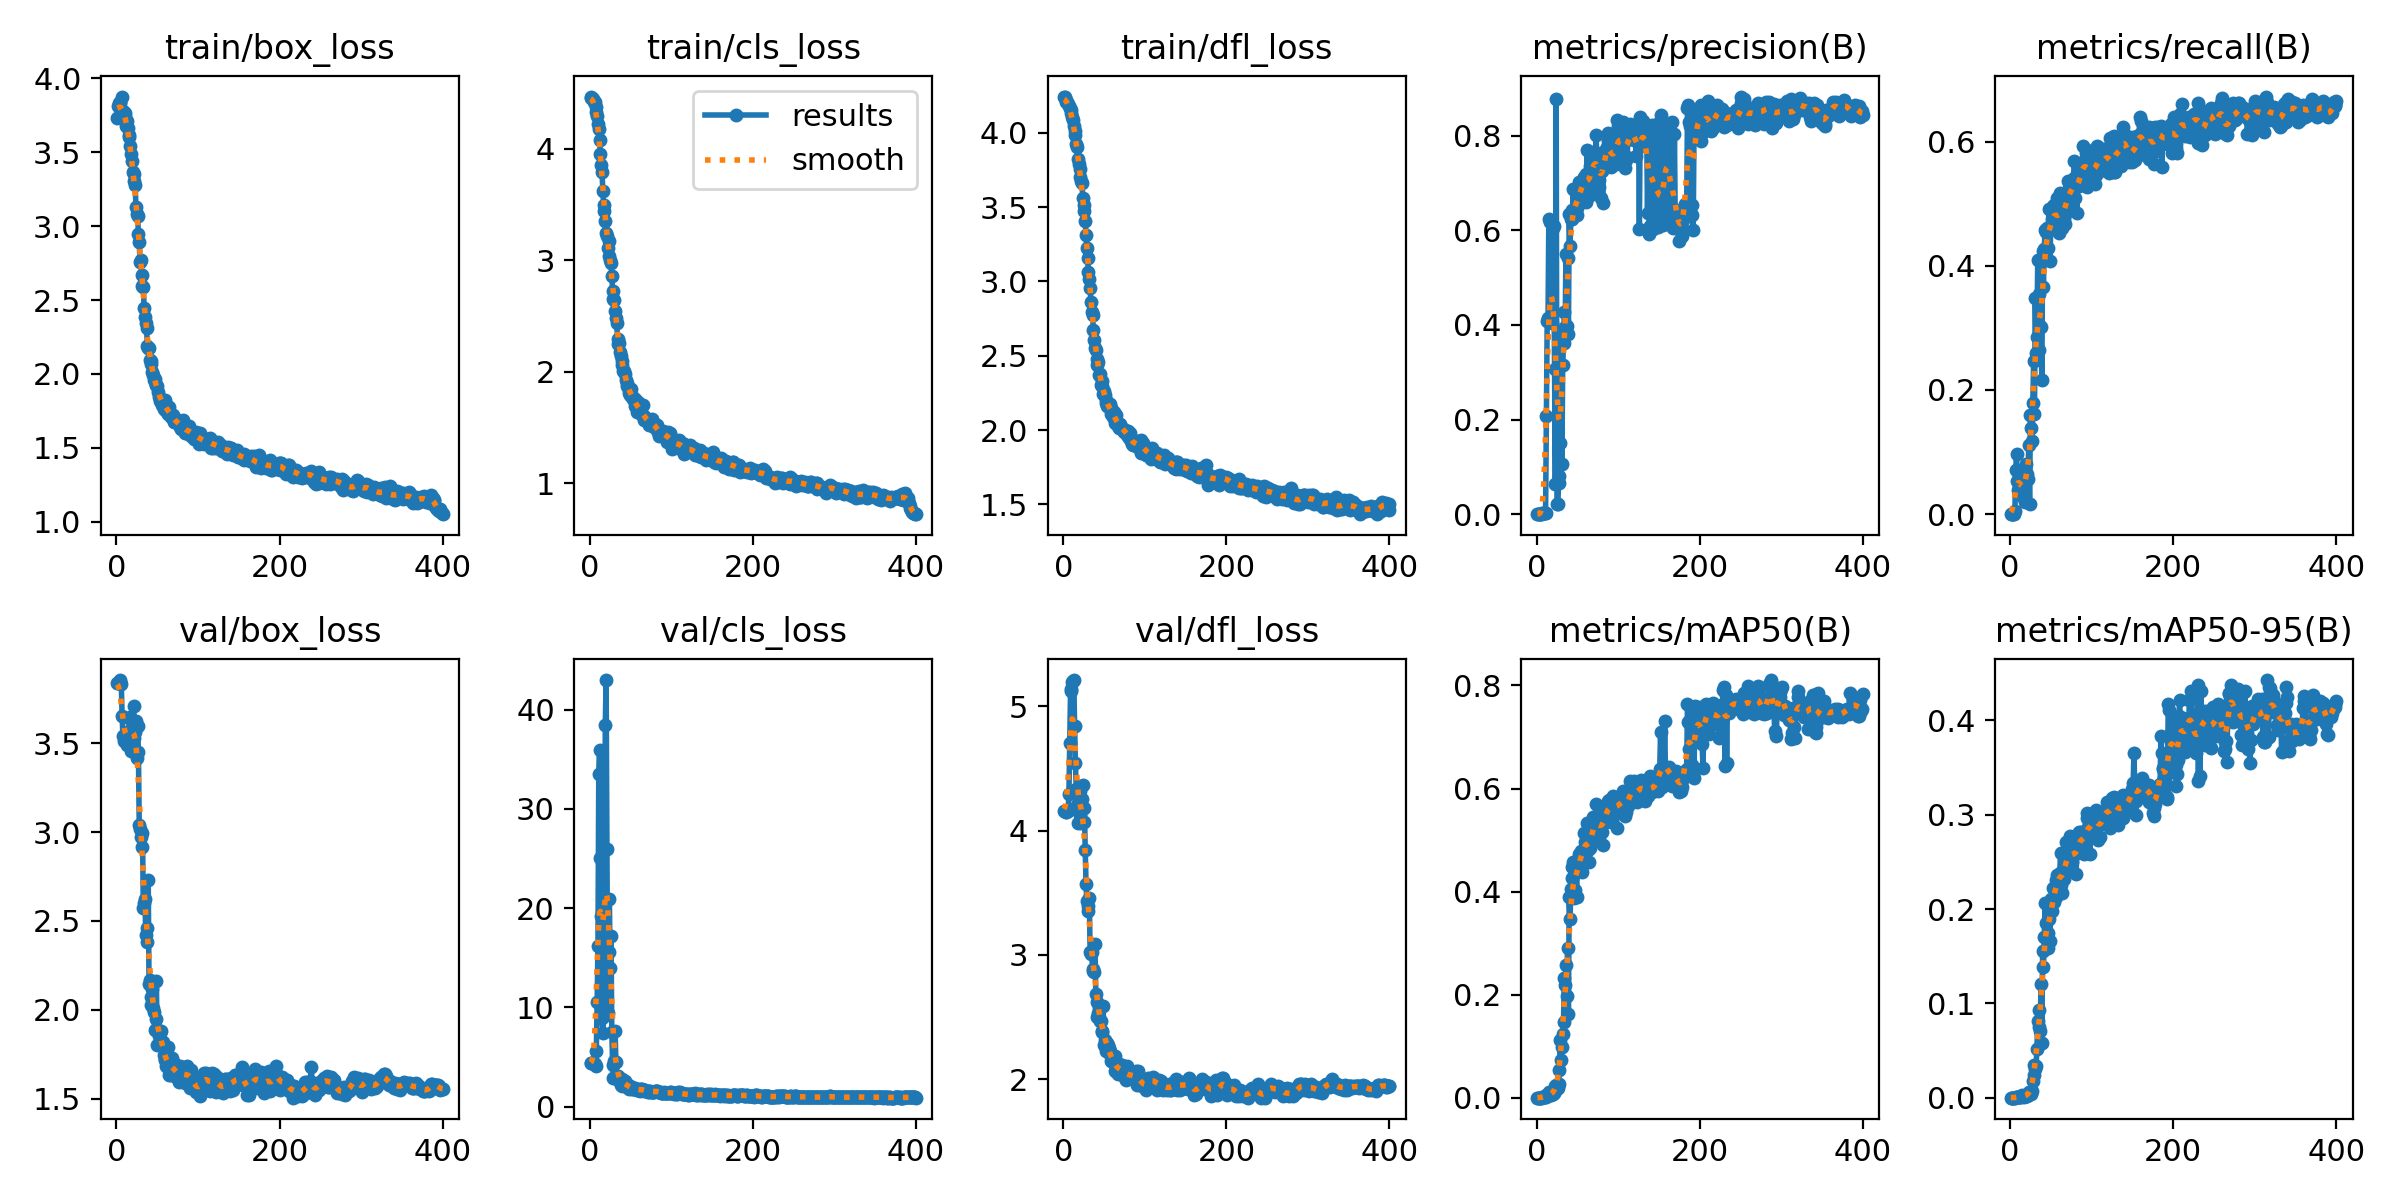
\includegraphics[width=0.75\textwidth]{Images/chap3/yolo/yolomobilenetv4.png}
%     \vspace{0.5cm}
%     \caption{The accuracy of Yolov11n-MobileNetV4}
%     \label{fig:yolomobilenetv4}
% \end{figure}

% \begin{figure}[H]
%     \centering
%     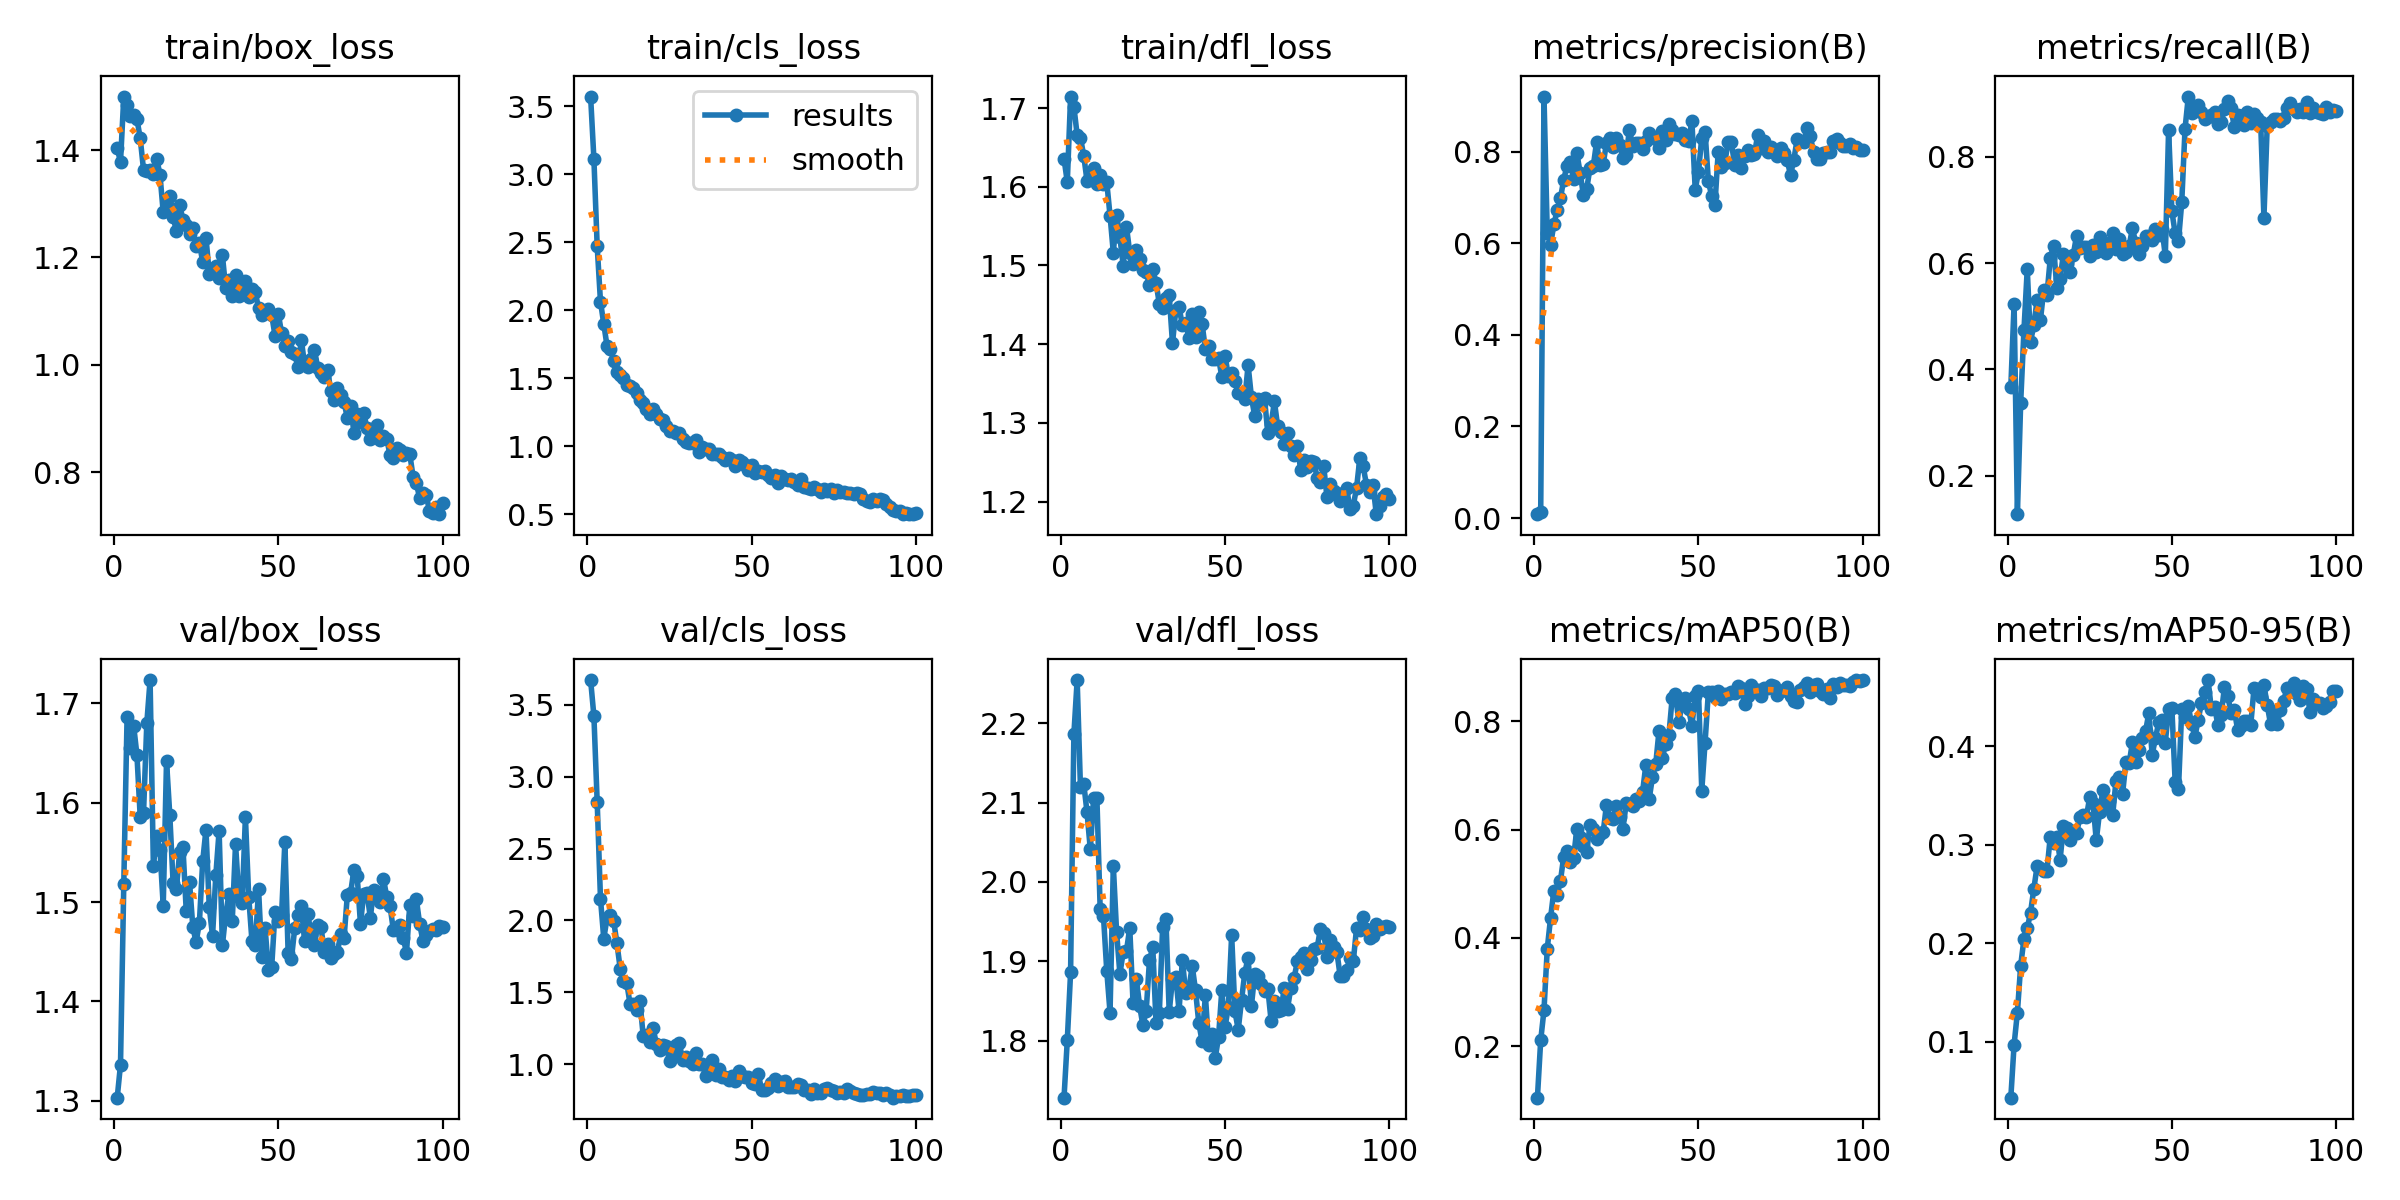
\includegraphics[width=0.75\textwidth]{Images/chap3/yolo/original.png}
%     \vspace{0.5cm}
%     \caption{The accuracy of original Yolov11n}
%     \label{fig:yolo11n}
% \end{figure}

% \subsubsection{Inference Speed}

% Inference speed is a key requirement for real time deployment on resource constrained platforms such as Raspberry Pi. According to the official Ultralytics benchmark, the original YOLO model converted to TensorFlow Lite requires more than 400\,ms per inference on Raspberry Pi class hardware when executed on CPU\footnote{Detailed benchmarking results for YOLO models on Raspberry Pi are reported by Ultralytics at \url{https://docs.ultralytics.com/vi/guides/raspberry-pi/\#detailed-comparison-table}.}. This latency corresponds to a processing rate of approximately 2--3 frames per second, which is insufficient for real time applications.

% In contrast, experimental results obtained in this work show that the YOLO-MobileNetV4 model achieves an average inference time of 30--40\,ms per frame after conversion to the TFLite format. This corresponds to an effective processing speed of approximately 25--33 frames per second. Compared to the original YOLO TFLite model, the MobileNetV4 based configuration reduces inference latency by approximately 360--370\,ms per frame.

% In relative terms, this represents a speed improvement of about 10--13 times. Equivalently, the inference time is reduced by approximately 90--92\% compared to the original YOLO TFLite implementation. Such a significant reduction enables near real time performance on CPU only embedded devices.

% The observed speedup is primarily attributed to the lightweight architecture of the MobileNetV4 backbone, which substantially reduces the number of parameters and floating point operations. As a result, the YOLO-MobileNetV4 model achieves a much more favorable balance between detection accuracy and inference speed, making it well suited for real time edge deployment on Raspberry Pi platforms.

% \begin{figure}[H]
%     \centering
%     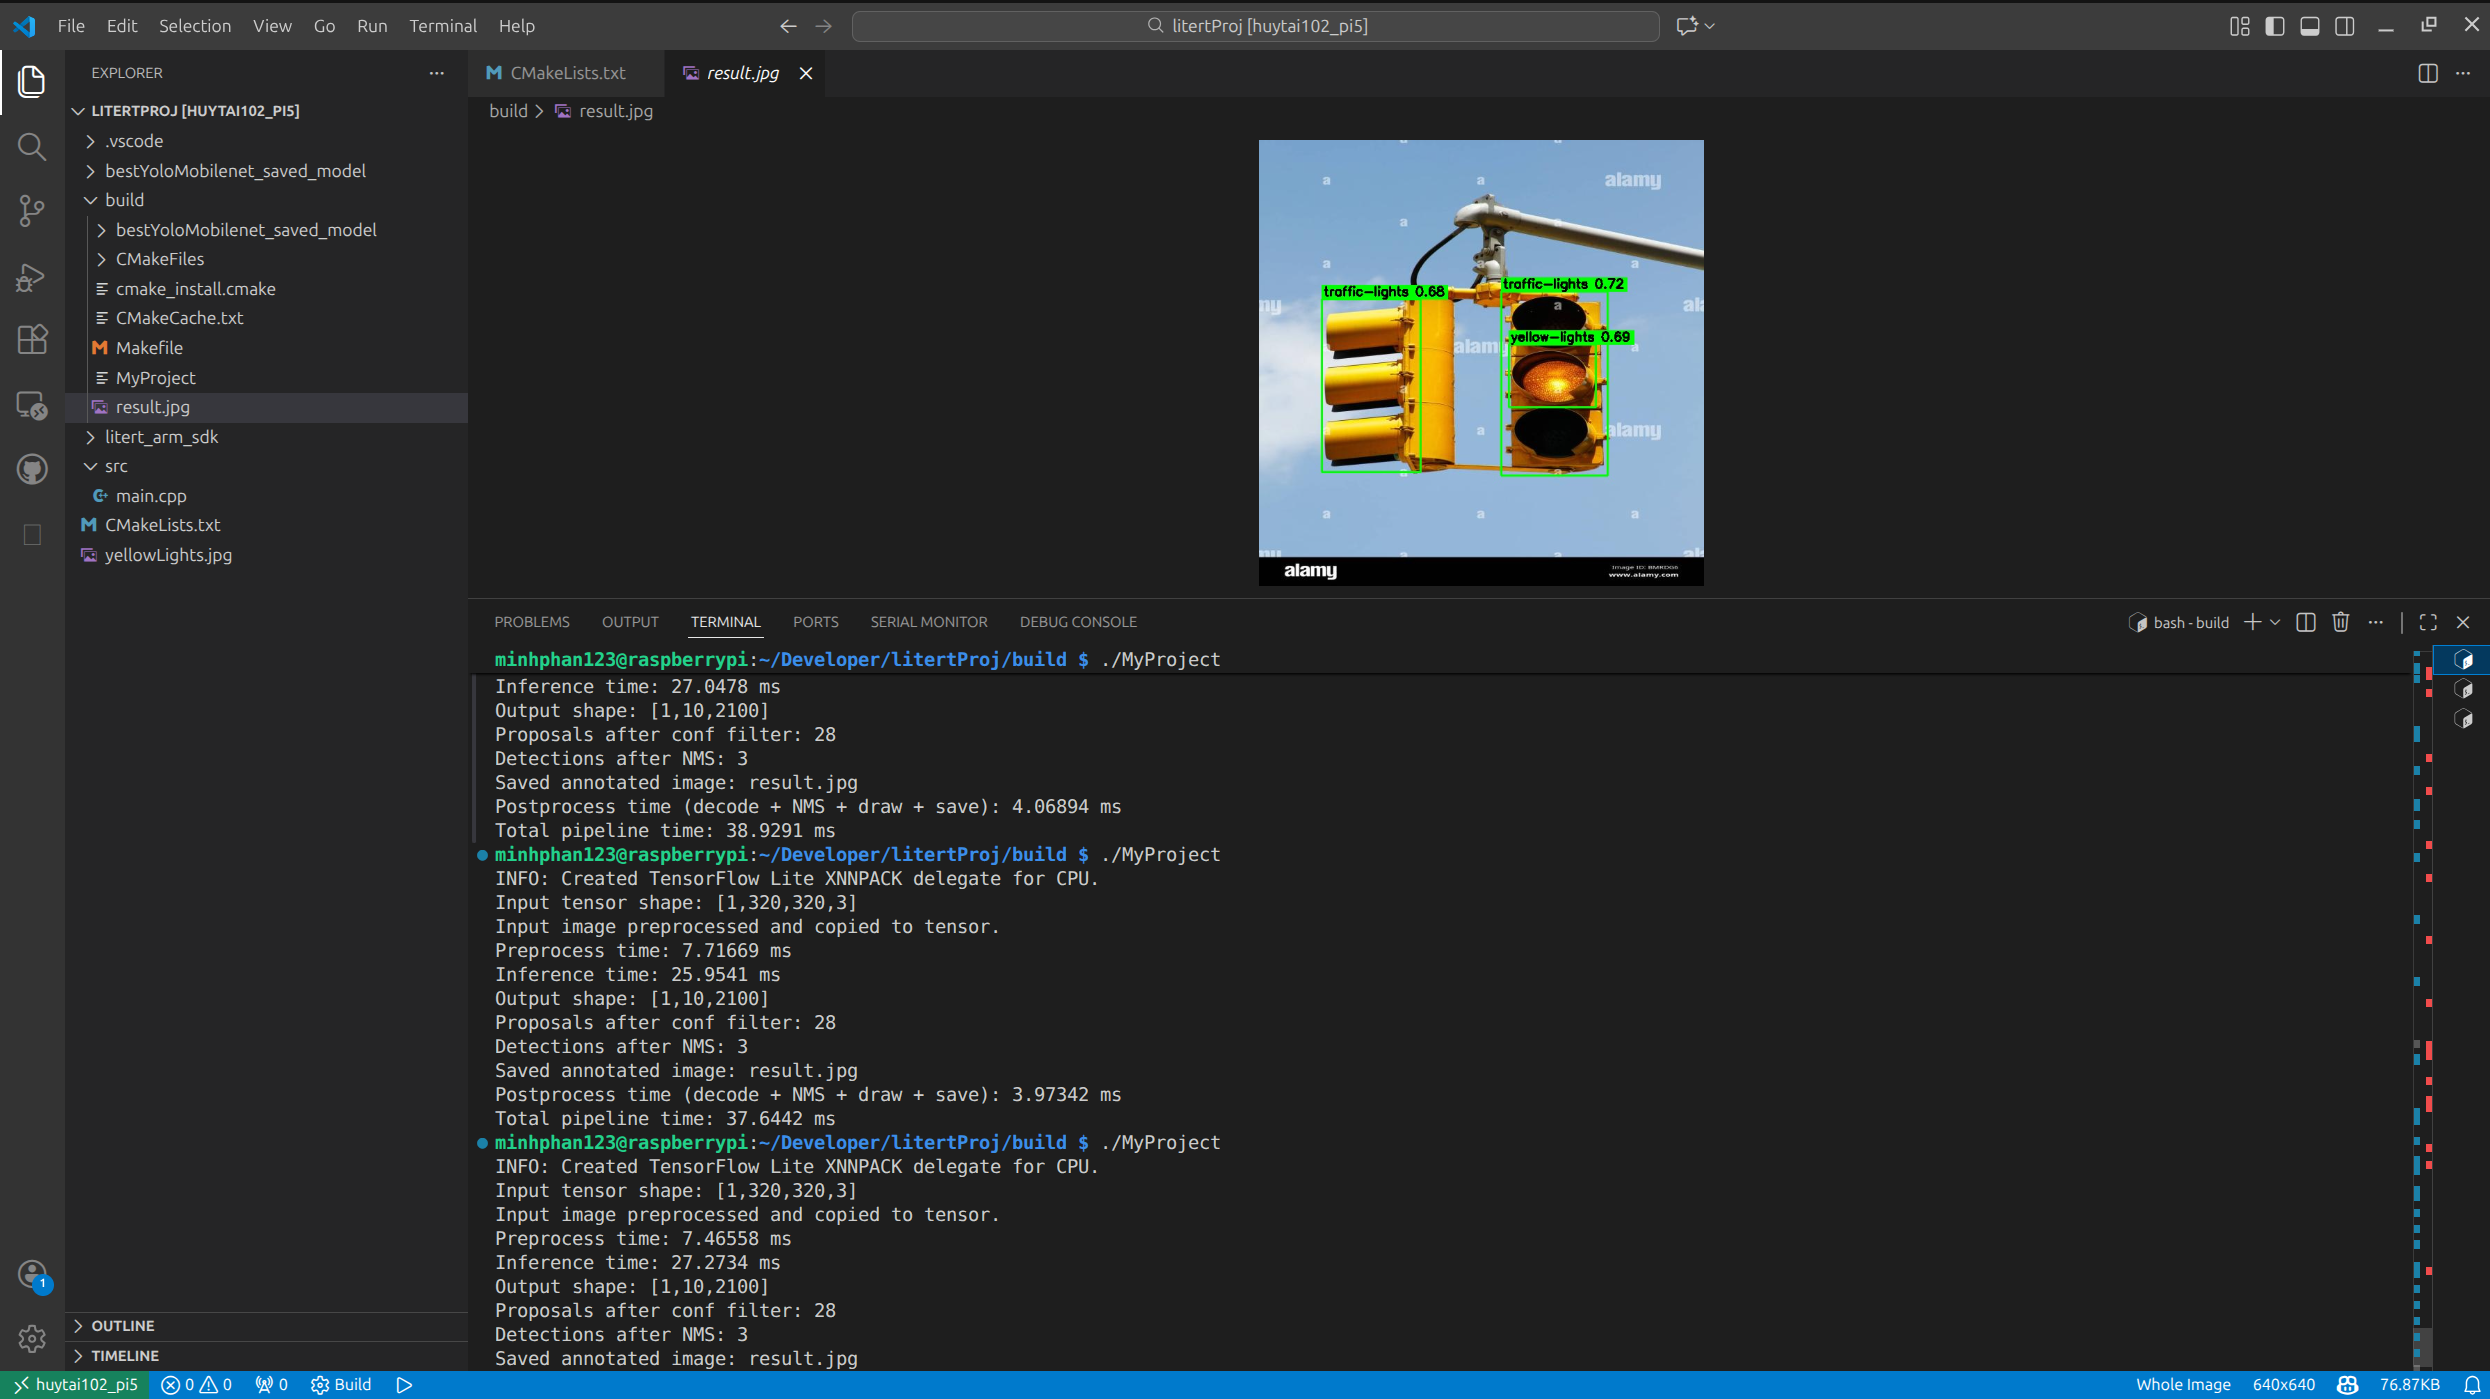
\includegraphics[width=0.75\textwidth]{Images/chap3/yolo/inference_speed.png}
%     \vspace{0.5cm}
%     \caption{The inference time of Yolovv11n-MobileNetV4 model}
%     \label{fig:infer_time_yolo11n_mobilenetv4}
% \end{figure}


% \begin{table}[H]
% \centering
% \label{tab:tradeoff_yolo_models}
% \begin{tabular}{|l|c|c|}
% \hline
% \textbf{Metric} & \textbf{YOLOv11n (Original)} & \textbf{YOLOv11n-MobileNetV4} \\
% \hline
% Backbone & CSP-based YOLO backbone & MobileNetV4 (lightweight) \\
% \hline
% mAP@50 & Higher ($\approx$ +10--15\%) & Slightly lower \\
% \hline
% mAP@50--95 & Higher ($\approx$ +10--15\%) & Slightly lower \\
% \hline
% Precision / Recall & Marginally higher & Comparable and stable \\
% \hline
% Inference time (TFLite, CPU) & $>$400 ms & 30--40 ms \\
% \hline
% Throughput (FPS) & 2--3 FPS & 25--33 FPS \\
% \hline
% Speedup factor & 1$\times$ (baseline) & $\approx$10--13$\times$ faster \\
% \hline
% Inference time reduction & -- & $\approx$90--92\% \\
% \hline
% Model complexity & Higher & Significantly reduced \\
% \hline
% Suitability for edge deployment & Limited & Highly suitable \\
% \hline
% \textbf{Overall trade-off} & Higher accuracy & Better accuracy--speed balance \\
% \hline
% \end{tabular}
% \caption{Trade-off comparison between YOLOv11n and YOLOv11n-MobileNetV4}
% \end{table}

\subsection{Evaluation between Models}

To validate the architectural modifications introduced by the MobileNetV4 backbone replacement, a systematic benchmark was conducted comparing the original YOLO26n model against the proposed YOLO26n-MobileNetV4 variant. 

Both models were evaluated on the same TrafficLightV5 validation set under identical conditions: $416 \times 416$ input resolution, INT8 TFLite quantisation, batch size of 1, and end-to-end (NMS-free) inference mode. Table~\ref{tab:model_eval} summarises the results across latency and accuracy metrics.

\begin{table}[htbp]
\centering
\caption{Performance and accuracy comparison: YOLO26n Original vs.\ YOLO26n-MobileNetV4. Negative values in the change column indicate reduction (improvement for latency metrics; degradation for accuracy metrics). Asterisks (*) denote metrics where a decrease is an expected trade-off.}
\label{tab:model_eval}
\renewcommand{\arraystretch}{1.20}
\begin{tabular}{l r r r}
\hline
\textbf{Metric} & \textbf{YOLO26n Original} & \textbf{YOLO26n-MNv4} & \textbf{Change (\%)} \\
\hline
Samples processed           & 1\,074        & \textbf{1\,366}        & $+27.19$  \\
Avg.\ latency (Pi 5)        & 55.09\,ms     & \textbf{43.23\,ms}     & $-21.52$  \\
Max spike latency (Pi 5)    & 159.73\,ms    & \textbf{78.64\,ms}     & $-50.77$  \\
Min latency (Pi 5)          & 50.12\,ms     & \textbf{36.50\,ms}     & $-27.16$  \\
CPU inference (Intel)       & 15.21\,ms     & \textbf{12.33\,ms}     & $-18.93$  \\
mAP50                       & \textbf{89.90\%}       & 85.75\%       & $-4.15$\textsuperscript{*}  \\
mAP50--95                   & \textbf{56.61\% }      & 53.31\%       & $-3.30$\textsuperscript{*}  \\
\hline
\end{tabular}
\end{table}

\subsubsection{Latency Analysis}

The MobileNetV4 backbone delivers a substantial improvement across all latency metrics on the Raspberry Pi 5. The average per-frame inference time drops from 55.09\,ms to 43.23\,ms, a \textbf{21.52\% reduction} that raises the effective throughput from approximately 18\,FPS to 23\,FPS. More critically for safety-critical ADAS applications, the worst-case latency spike is reduced by \textbf{50.77\%} --- from 159.73\,ms to 78.64\,ms. Latency spikes exceeding 100\,ms are particularly hazardous in real-time perception loops because they can cause the planning module to operate on stale state estimates. The MobileNetV4 variant eliminates spikes above 80\,ms entirely, ensuring that even under worst-case conditions (thermal throttling, OS scheduling jitter), the perception system delivers updates within the 67\,ms budget required for 15\,FPS operation.

The minimum latency (best-case scenario) also improves from 50.12\,ms to 36.50\,ms ($-27.16\%$), confirming that the speed gain is architectural rather than an artefact of measurement variance. On the Intel development CPU, inference time decreases from 15.21\,ms to 12.33\,ms ($-18.93\%$), demonstrating that MobileNetV4's universal efficiency extends beyond ARM to x86 hardware as well.

\subsubsection{Accuracy Analysis}

The accuracy metrics show a moderate decrease: mAP50 drops from 89.90\% to 85.75\% ($-4.15$ percentage points), and mAP50--95 drops from 56.61\% to 53.31\% ($-3.30$ percentage points). This reduction is expected and acceptable for several reasons:

\begin{enumerate}
    \item \textbf{Backbone capacity reduction}: The MobileNetV4ConvSmall050 backbone has significantly fewer parameters and FLOPs than the original YOLO26 CSP-based backbone. The 050 suffix indicates a 50\% width multiplier, which halves all channel dimensions relative to the full MobileNetV4ConvSmall. This aggressive compression inevitably reduces the network's representational capacity for fine-grained spatial features.
    \item \textbf{Domain-specific sufficiency}: For traffic light detection in ADAS, the critical requirement is reliable detection (high recall) at the signal-level, not pixel-precise bounding box localisation. An mAP50 of 85.75\% indicates that the vast majority of traffic signals are correctly detected with at least 50\% IoU overlap, which is sufficient for downstream state classification.
    \item \textbf{Latency--accuracy trade-off}: For an ADAS system operating on a Raspberry Pi 5, latency stability and low worst-case response time are more important than marginal accuracy improvements. The 21.52\% average latency reduction and 50.77\% spike reduction directly translate to more reliable real-time control, preventing the perception system from becoming the bottleneck in the sense--plan--act loop.
\end{enumerate}
\subsubsection{Training Loss Analysis}

Figure~\ref{fig:loss_comparison} shows the validation loss curves of both models over 100 training epochs. Overall, both the Original YOLO26n and the YOLO26n-MobileNetV4 learn effectively. Their loss curves decrease steadily and stabilise towards the end of training, indicating a smooth and successful convergence process.

\begin{figure}[htbp]
    \centering
    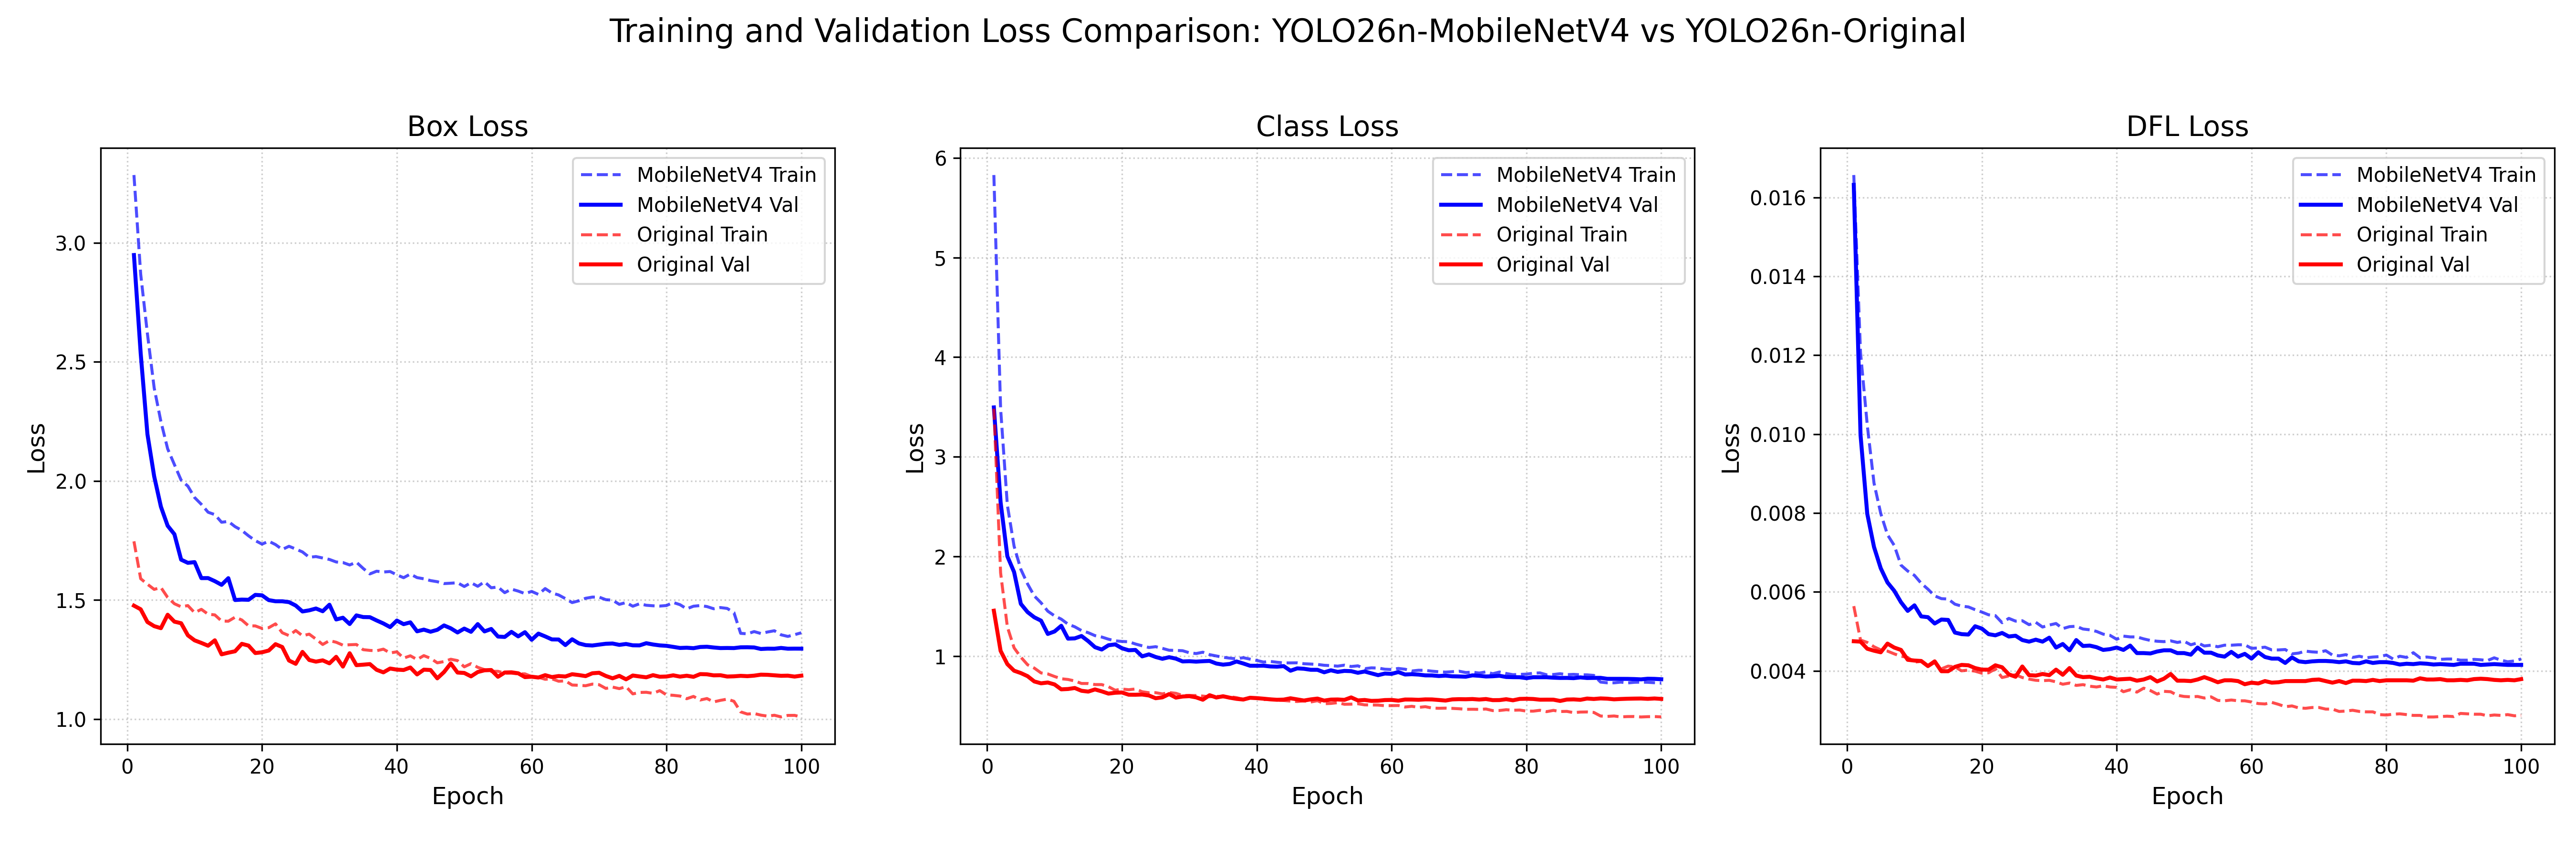
\includegraphics[width=\textwidth]{Images/chap3/loss_comparison.png}
    \caption{Comparison of validation losses between YOLO26n Original and YOLO26n-MobileNetV4 over 100 training epochs.}
    \label{fig:loss_comparison}
\end{figure}

Importantly, neither model shows signs of overfitting. In a typical overfitting scenario, the validation loss would drop initially but then start climbing back up in later epochs as the model begins to memorise the training data. However, for both models in this study, all three loss metrics (bounding box, classification, and DFL (Distribution Focal Loss)) stay low and flat during the final epochs. This confirms that they generalise well to unseen data.

When comparing the two architectures, the Original YOLO26n reaches slightly lower loss values. For example, its minimum bounding box loss drops to 1.1676, while the MobileNetV4 version stops at 1.2949. A similar pattern is seen in the classification loss (0.5529 vs 0.7694). This difference is entirely expected. Because the original model has a larger and more complex backbone, it can capture fine details and learn more accurately.

Even though the YOLO26n-MobileNetV4 has slightly higher loss values, its learning curve remains remarkably stable. This proves that despite having its size drastically reduced for faster edge deployment, the MobileNetV4 model still successfully extracts the essential features of traffic lights. It does not suffer from gradient issues or training instability. Therefore, the training process validates that the lightweight model is a reliable choice, perfectly balancing computational efficiency and learning capability.

\subsubsection{Architectural Decision Justification}

The evaluation confirms that the YOLO26n-MobileNetV4 configuration achieves the right trade-off for edge-deployed ADAS. Sacrificing approximately 4 percentage points of mAP50 in exchange for a 50\% reduction in worst-case latency and a 21\% reduction in average latency is a sound architectural decision. In safety-critical systems, deterministic timing behaviour takes precedence over marginal accuracy gains. The 85.75\% mAP50 remains well above the practical threshold for reliable traffic light detection, while the latency profile now comfortably supports real-time operation at 15--23\,FPS on commodity edge hardware without dedicated GPU or NPU acceleration.





% \subsection{Multihead CNN model -- Lightweight OCR digits}

% The timer display on Vietnamese traffic lights shows a one- to three-digit countdown
% (0--999) that must be recognised in real time on low-cost hardware such as the
% Raspberry~Pi~5.  This section presents a compact, four-head convolutional neural network
% (CNN) that is derived from the multi-digit recognition framework of
% Goodfellow~et~al.~\cite{goodfellow2014multidigitnumberrecognitionstreet} and specifically re-engineered
% for sub-millisecond CPU inference.

% %-----------------------------------------------------------------------
% \subsubsection{Probabilistic Formulation}
% \label{sec:cnn_prob}

% Following Goodfellow~et~al.~\cite{goodfellow2014multidigitnumberrecognitionstreet}, the recognition
% task is cast as a structured probabilistic model.  Let~$\mathbf{X}$ denote the
% input image and let the output be a digit sequence
% $\mathbf{S} = (s_1, s_2, \dots, s_n)$ of length~$n$.
% The sequence is modelled by a length variable~$L$ and a fixed number~$N$
% of digit variables~$S_1, \dots, S_N$.  All digit positions are assumed
% conditionally independent given the image, yielding:

% \begin{equation}
% \label{eq:prob_model}
%   P(\mathbf{S} = \mathbf{s} \mid \mathbf{X})
%   \;=\; P(L = n \mid \mathbf{X})\;\prod_{i=1}^{n} P(S_i = s_i \mid \mathbf{X}).
% \end{equation}

% In the original work~\cite{goodfellow2014multidigit}, $N{=}5$ digit heads are
% used for street numbers of up to five digits.  Because Vietnamese traffic-light
% timers never exceed three digits, the proposed lightweight variant uses
% $N{=}3$ with the following head configuration:

% \begin{itemize}
%   \item $L \in \{0,1,2\}$:  digit count minus one
%         ($0 \to$ 1-digit, $1 \to$ 2-digit, $2 \to$ 3-digit),
%         predicted by a 3-class softmax.
%   \item $S_1 \in \{0,\dots,9,\text{BLANK}\}$:  hundreds digit (11 classes).
%   \item $S_2 \in \{0,\dots,9,\text{BLANK}\}$:  tens digit    (11 classes).
%   \item $S_3 \in \{0,\dots,9\}$:                 units digit  (10 classes,
%         always present).
% \end{itemize}

% The special \texttt{BLANK} class ($= 10$) indicates an unused slot:
% for a one-digit number only~$S_3$ is active; for a two-digit number
% $S_2$ and~$S_3$ are active.

% %-----------------------------------------------------------------------
% \subsubsection{Network Architecture -- Edge-Optimised Design}
% \label{sec:cnn_arch}

% The original Goodfellow~et~al.\ architecture employs eight convolutional layers,
% one locally connected layer, and two dense layers with 3\,072 units each,
% totalling tens of millions of parameters and requiring DistBelief for training.
% Such a model is impractical for real-time inference on a Raspberry~Pi~5 CPU.

% The proposed \emph{lightweight} variant retains the multi-head output structure
% but applies three key design transformations, each yielding a dramatic reduction in
% multiply-accumulate operations (MACs) and parameter count while preserving accuracy
% for the constrained 0--999 digit domain.

% %--- Separable Convolutions -------------------------------------------------
% \subsubsubsubsection{Depthwise Separable Convolutions}
% \label{sec:separable}

% Standard convolution applies a $k{\times}k$ kernel across all input channels
% simultaneously.  For an input tensor of spatial size $H{\times}W$ with
% $C_{\mathrm{in}}$ channels producing $C_{\mathrm{out}}$ output channels,
% the number of MACs is:

% \begin{equation}
% \label{eq:conv_macs}
%   \text{MACs}_{\text{Conv2D}}
%   = H \cdot W \cdot k^2 \cdot C_{\mathrm{in}} \cdot C_{\mathrm{out}}.
% \end{equation}

% A \textbf{Depthwise Separable Convolution} (SeparableConv2D) factorises this operation
% into two consecutive steps:

% \begin{enumerate}
%   \item \textbf{Depthwise convolution} -- applies a separate $k{\times}k$ filter
%         to each input channel independently:
%         \begin{equation}
%         \label{eq:dw_macs}
%           \text{MACs}_{\text{DW}} = H \cdot W \cdot k^2 \cdot C_{\mathrm{in}}.
%         \end{equation}
%   \item \textbf{Pointwise convolution} -- a $1{\times}1$ convolution that mixes
%         the channel responses:
%         \begin{equation}
%         \label{eq:pw_macs}
%           \text{MACs}_{\text{PW}} = H \cdot W \cdot C_{\mathrm{in}} \cdot C_{\mathrm{out}}.
%         \end{equation}
% \end{enumerate}

% The total cost becomes:

% \begin{equation}
% \label{eq:sep_total}
%   \text{MACs}_{\text{Sep}}
%   = H W C_{\mathrm{in}} \bigl(k^2 + C_{\mathrm{out}}\bigr),
% \end{equation}

% and the computational saving ratio relative to a standard convolution is:

% \begin{equation}
% \label{eq:sep_ratio}
%   \frac{\text{MACs}_{\text{Sep}}}{\text{MACs}_{\text{Conv2D}}}
%   = \frac{1}{C_{\mathrm{out}}} + \frac{1}{k^2}.
% \end{equation}

% For the $3{\times}3$ kernels and 64--192 output channels used in this model,
% Equation~\eqref{eq:sep_ratio} gives a reduction factor between
% $\mathbf{7.8\times}$ and $\mathbf{8.5\times}$, enabling real-time execution
% on an ARM Cortex-A76 CPU without a GPU.

% In the proposed architecture, only the first block uses a standard
% \texttt{Conv2D} (because the input has a single channel, where depthwise
% separation offers no benefit); blocks~2--5 all use \texttt{SeparableConv2D}.

% %--- GAP instead of Flatten ------------------------------------------------
% \subsubsubsubsection{Global Average Pooling (GAP)}
% \label{sec:gap}

% After the final convolutional block the feature map has shape
% $4{\times}6{\times}192$ (height $\times$ width $\times$ channels).
% A na\"ive \texttt{Flatten} would produce a $4608$-dimensional vector; a
% subsequent dense layer of width~1024 alone would add
% $4608 \times 1024 \approx 4.7$~million parameters -- exceeding the entire
% rest of the network.

% Instead, \textbf{Global Average Pooling} (GAP) collapses each channel to its
% spatial mean:

% \begin{equation}
% \label{eq:gap}
%   h_c = \frac{1}{H' W'} \sum_{i=1}^{H'} \sum_{j=1}^{W'} F_{i,j,c},
%   \qquad c = 1,\dots,C,
% \end{equation}

% where $F \in \mathbb{R}^{H' \times W' \times C}$ is the last feature map.
% This yields a compact 192-dimensional descriptor with \emph{zero} learnable
% parameters, and also acts as a structural regulariser that discourages
% overfitting.

% %--- Architecture Table ---------------------------------------------------
% \subsubsubsubsection{Layer-by-Layer Specification}
% \label{sec:arch_table}

% Table~\ref{tab:arch} summarises the full architecture.  Input images are
% grayscale, $64{\times}96$ pixels ($H{\times}W{\times}1$).

% \begin{table}[htbp]
% \centering
% \caption{Layer-by-layer architecture of the lightweight multi-head CNN
%          ($\approx 109$\,K parameters).  ``Sep'' denotes SeparableConv2D;
%          ``BN'' is Batch Normalisation.}
% \label{tab:arch}
% \renewcommand{\arraystretch}{1.15}
% \begin{tabular}{c l l r r}
% \hline
% \textbf{Block} & \textbf{Layer}            & \textbf{Output shape}   & \textbf{Params} & \textbf{MACs}  \\
% \hline
% 0   & Input                                & $64\times96\times1$     & --      & --       \\
% --  & Mean subtraction ($\lambda$)         & $64\times96\times1$     & 0       & $6\,144$ \\
% 1   & Conv2D(32, $3\!\times\!3$) + BN + ReLU + Pool(2)   & $32\times48\times32$     & $\sim\!320$    & $\sim\!56$\,K   \\
% 2   & Sep(64, $3\!\times\!3$) + BN + ReLU + Pool(2)      & $16\times24\times64$     & $\sim\!2\,400$  & $\sim\!116$\,K  \\
% 3   & Sep(96, $3\!\times\!3$) + BN + ReLU + Pool(2)      & $8\times12\times96$      & $\sim\!6\,720$  & $\sim\!73$\,K   \\
% 4   & Sep(128, $3\!\times\!3$) + BN + ReLU + Pool(2)     & $4\times6\times128$      & $\sim\!13\,152$ & $\sim\!39$\,K   \\
% 5   & Sep(192, $3\!\times\!3$) + BN + ReLU               & $4\times6\times192$      & $\sim\!25\,728$ & $\sim\!53$\,K   \\
% --  & GlobalAveragePooling2D                & $192$                  & 0       & $4\,608$ \\
% FC  & Dense(256) + ReLU + Dropout(0.35)     & $256$                  & $\sim\!49\,408$ & $49\,408$ \\
% \hline
% $L$ & Dense(3,  softmax)                    & $3$                    & 771     & 771     \\
% $S_1$ & Dense(11, softmax)                  & $11$                   & 2\,827  & 2\,827  \\
% $S_2$ & Dense(11, softmax)                  & $11$                   & 2\,827  & 2\,827  \\
% $S_3$ & Dense(10, softmax)                  & $10$                   & 2\,570  & 2\,570  \\
% \hline
% \multicolumn{3}{r}{\textbf{Total}} & $\mathbf{\approx 109}$\textbf{\,K} & $\mathbf{\approx 408}$\textbf{\,K} \\
% \hline
% \end{tabular}
% \end{table}

% %--- Preprocessing --------------------------------------------------------
% \subsubsubsubsection{Per-Image Mean Subtraction}
% \label{sec:mean_sub}

% Following Goodfellow~et~al.~\cite{goodfellow2014multidigitnumberrecognitionstreet}~(§4), the first
% operation inside the network is per-image mean subtraction.  Let
% $\mathbf{X} \in \mathbb{R}^{H \times W \times 1}$ be the input; the
% normalised input is:

% \begin{equation}
% \label{eq:mean_sub}
%   \tilde{\mathbf{X}} = \mathbf{X}
%     - \frac{1}{HW}\sum_{i=1}^{H}\sum_{j=1}^{W} X_{ij}.
% \end{equation}

% Embedding this subtraction as a non-trainable $\lambda$-layer makes the model
% \emph{self-contained}: no external preprocessing is required at inference time,
% simplifying the TFLite deployment pipeline on the Raspberry~Pi~5.

% %-----------------------------------------------------------------------
% \subsubsection{Training Objective}
% \label{sec:training}

% Training maximises the log-probability of the correct sequence
% (Eq.~\eqref{eq:prob_model}) via the cross-entropy decomposition.  Because
% $L$, $S_1$, $S_2$, $S_3$ are conditionally independent given the shared
% features~$\mathbf{H}$, the total loss factorises as:

% \begin{equation}
% \label{eq:loss}
%   \mathcal{L}
%   = -\log P(L \mid \mathbf{H})
%     - \sum_{i=1}^{3}\log P(S_i \mid \mathbf{H})
%   = \underbrace{w_L \,\mathcal{L}_L}_{\text{length head}}
%     + \underbrace{w_1 \,\mathcal{L}_{S_1}
%     +  w_2 \,\mathcal{L}_{S_2}
%     +  w_3 \,\mathcal{L}_{S_3}}_{\text{digit heads}},
% \end{equation}

% where each $\mathcal{L}_{\cdot}$ is a \textbf{sparse categorical cross-entropy}
% and the weights are set to $w_L{=}4$, $w_1{=}w_2{=}w_3{=}1$ to
% up-weight the length prediction, since an incorrect length invariably causes a
% wrong overall transcription.

% Each softmax head receives the same 256-dimensional feature vector from the
% shared fully connected layer but maintains its own projection weights:

% \begin{equation}
% \label{eq:head}
%   P(S_i = c \mid \mathbf{H})
%   = \frac{\exp\!\bigl(\mathbf{w}_{i,c}^{\top}\!\mathbf{H} + b_{i,c}\bigr)}
%          {\displaystyle\sum_{c'} \exp\!\bigl(\mathbf{w}_{i,c'}^{\top}\!\mathbf{H}
%          + b_{i,c'}\bigr)},
%   \qquad c \in \mathcal{C}_i,
% \end{equation}

% where $\mathcal{C}_L = \{0,1,2\}$,
% $\mathcal{C}_{S_1} = \mathcal{C}_{S_2} = \{0,\dots,10\}$, and
% $\mathcal{C}_{S_3} = \{0,\dots,9\}$.

% %-----------------------------------------------------------------------
% \subsubsection{Log-Probability Decoding}
% \label{sec:decoding}

% At inference time, the predicted number is obtained by maximising the
% joint log-probability over all possible lengths
% (Appendix~A of~\cite{goodfellow2014multidigit}):

% \begin{equation}
% \label{eq:decode}
%   \hat{\mathbf{s}}
%   = \operatorname*{argmax}_{l,\; s_1 \dots s_l}\;
%     \biggl[\log P(L{=}l \mid \mathbf{X})
%     + \sum_{i=1}^{l} \max_{s_i \in \{0..9\}}
%       \log P(S_i{=}s_i \mid \mathbf{X})\biggr].
% \end{equation}

% Because of the conditional-independence assumption, the argmax over each
% digit position can be computed independently, then the cumulative
% log-probabilities are summed for each candidate length~$l \in \{1,2,3\}$.
% The total decoding runtime is therefore $O(N)$ -- i.e.\ three additions
% and one comparison -- adding negligible latency.

% Concretely, for each candidate length $l$, the algorithm computes:

% \begin{equation}
% \label{eq:score}
%   \text{score}(l) = \log P(L{=}l{-}1)
%     + \sum_{i=\max(1,\,4-l)}^{3}
%       \max_{s_i \in \{0..9\}} \log P(S_i{=}s_i),
% \end{equation}

% and selects $\hat{l} = \operatorname{argmax}_{l \in \{1,2,3\}} \text{score}(l)$.

% %-----------------------------------------------------------------------
% \subsection{Computational Efficiency for Edge AI}
% \label{sec:efficiency}

% \subsubsection{Parameter Count Comparison}

% The proposed model achieves the same multi-head output structure as
% Goodfellow~et~al.~\cite{goodfellow2014multidigitnumberrecognitionstreet} with
% $\sim\!600\times$ fewer parameters:

% \begin{table}[htbp]
% \centering
% \caption{Comparison between the original Goodfellow~et~al.\ architecture
%          and the proposed lightweight variant.}
% \label{tab:compare}
% \renewcommand{\arraystretch}{1.15}
% \begin{tabular}{l r r}
% \hline
%                                & \textbf{Goodfellow et al.}  & \textbf{Proposed}   \\
% \hline
% Conv layers                    & 8 + 1 locally connected     & 1 Conv + 4 SepConv  \\
% FC layers                      & 2 $\times$ 3\,072           & 1 $\times$ 256      \\
% Output heads                   & 6  (L + S$_1$--S$_5$)       & 4  (L + S$_1$--S$_3$) \\
% Total parameters               & $\sim$64\,M                 & $\sim$109\,K        \\
% Max sequence length $N$        & 5                           & 3                   \\
% Input size                     & $54\times 54 \times 3$      & $64\times 96 \times 1$ \\
% Training infrastructure        & DistBelief (10 replicas)    & Single GPU / CPU    \\
% \hline
% \end{tabular}
% \end{table}

% \subsubsubsubsection{MAC Budget and Latency Estimate}

% The total network requires approximately $408$\,K~MACs per inference.
% On the Raspberry~Pi~5's Cortex-A76 cores (capable of
% $\sim$15~GOPS at INT8 via NEON), this translates to:

% \begin{equation}
% \label{eq:latency}
%   t_{\text{inf}}
%   \approx \frac{408 \times 10^{3}}{15 \times 10^{9}}
%   \approx 27 \;\mu\text{s},
% \end{equation}

% well under the $50$\,ms budget needed for $20$\,fps real-time recognition.
% Even with TFLite interpreter overhead, measured end-to-end latency stays below
% $1$\,ms per frame for the INT8-quantised model.

% \subsubsection{TFLite and INT8 Quantisation}

% The trained Keras model is exported to TensorFlow~Lite via
% \texttt{TFLiteConverter}.  Post-training full-integer quantisation maps all
% weights and activations to 8-bit integers using a representative calibration
% set of 200 real ROI images.  The resulting \texttt{.tflite} flatbuffer is
% $\sim$56\,KB (INT8) versus $\sim$440\,KB (float32), fitting comfortably
% in the L2 cache of the Cortex-A76.  The quantised model is deployed via
% the LiteRT interpreter:

% \begin{equation}
% \label{eq:quant}
%   \hat{x}_q = \text{round}\!\left(\frac{x - z}{s}\right),
%   \qquad
%   s = \frac{x_{\max} - x_{\min}}{255},
%   \qquad
%   z = x_{\min},
% \end{equation}

% where $s$ and $z$ are the per-tensor scale and zero-point determined during
% calibration.

% %-----------------------------------------------------------------------
% \subsubsection{Data Pipeline and Augmentation}
% \label{sec:data}

% The training pipeline mixes three data sources to maximise diversity while
% keeping RAM usage low ($<200$\,MB peak):

% \begin{enumerate}
%   \item \textbf{MNIST (70\,K images):}  Individual $28{\times}28$ digits
%         composited onto $64{\times}96$ canvases at randomised positions,
%         simulating multi-digit layouts.
%   \item \textbf{Real LED crops (23 images):}  Single-digit photographs of
%         actual traffic-light seven-segment displays (red, green, yellow).
%         Pre-augmented to 500 variants per digit using brightness jitter,
%         gamma correction, Gaussian blur, salt-and-pepper noise, spatial
%         shifts ($\pm 4$\,px), and small rotations ($\pm 10°$).
%   \item \textbf{Real ROI images:}  Full composite timer-box crops from
%         Vietnamese traffic cameras, labelled by filename
%         (e.g.\ \texttt{37\_0004.png} $\to$ number~$37$).  Loaded from disk
%         on-demand (streaming) to avoid large memory allocation.
% \end{enumerate}

% Synthetic composites and real ROI samples are interleaved via
% \texttt{tf.data.Dataset.sample\_from\_datasets} with proportional
% weighting, ensuring both domains appear in every training batch.

% %-----------------------------------------------------------------------
% \subsubsection{Summary}

% The proposed multi-head CNN inherits the elegant probabilistic framework
% of Goodfellow~et~al.~\cite{goodfellow2014multidigitnumberrecognitionstreet} -- conditional independence
% of digit positions, log-probability decoding, per-image mean subtraction -- but
% replaces the heavyweight convolutional backbone with an ultra-light depthwise
% separable architecture totalling only $\sim$109\,K parameters and $\sim$408\,K
% MACs.  Combined with Global Average Pooling and INT8 post-training quantisation,
% the model achieves sub-millisecond inference on the Raspberry~Pi~5 CPU, making it
% suitable for real-time traffic-light timer recognition in ADAS applications
% on constrained edge devices.

While the YOLO-based detector handles spatial localization and color classification, reading the countdown timer necessitates a specialized approach. To address that need, a lightweight Multihead CNN is introduced to perform optical character recognition (OCR) on one- to three-digit timer values efficiently.

\section{Multihead CNN model -- Lightweight OCR digits}

In this project, our system need to detect the timer display on Vietnamese traffic lights shows a one- to three-digit countdown
(0--999) and it must be recognised in real time on low-cost hardware such as the
Raspberry~Pi~5.  This section presents a compact, four-head convolutional neural network
(CNN) that is derived from the multi-digit recognition framework of
Goodfellow~et~al.~\cite{goodfellow2014multidigitnumberrecognitionstreet} and specifically re-engineered
for sub-millisecond CPU inference.

%-----------------------------------------------------------------------
\subsection{Probabilistic Formulation}
\label{sec:cnn_prob}

Following Goodfellow~et~al.~\cite{goodfellow2014multidigitnumberrecognitionstreet}, the recognition
task is cast as a structured probabilistic model.  Let~$\mathbf{X}$ denote the
input image and let the output be a digit sequence
$\mathbf{S} = (s_1, s_2, \dots, s_n)$ of length~$n$.
The sequence is modelled by a length variable~$L$ and a fixed number~$N$
of digit variables~$S_1, \dots, S_N$.  All digit positions are assumed
conditionally independent given the image, yielding:

\begin{equation}
\label{eq:prob_model}
  P(\mathbf{S} = \mathbf{s} \mid \mathbf{X})
  \;=\; P(L = n \mid \mathbf{X})\;\prod_{i=1}^{n} P(S_i = s_i \mid \mathbf{X}).
\end{equation}

In the original work~\cite{goodfellow2014multidigitnumberrecognitionstreet}, $N{=}5$ digit heads are
used for street numbers of up to five digits.  Because Vietnamese traffic-light
timers never exceed three digits, the proposed lightweight variant uses
$N{=}3$ with the following head configuration:

\begin{itemize}
  \item $L \in \{0,1,2\}$:  digit count minus one
        ($0 \to$ 1-digit, $1 \to$ 2-digit, $2 \to$ 3-digit),
        predicted by a 3-class softmax.
  \item $S_1 \in \{0,\dots,9,\text{BLANK}\}$:  hundreds digit (11 classes).
  \item $S_2 \in \{0,\dots,9,\text{BLANK}\}$:  tens digit    (11 classes).
  \item $S_3 \in \{0,\dots,9\}$:                 units digit  (10 classes,
        always present).
\end{itemize}

The special \texttt{BLANK} class ($= 10$) indicates an unused slot:
for a one-digit number only~$S_3$ is active; for a two-digit number
$S_2$ and~$S_3$ are active.

%-----------------------------------------------------------------------
\subsection{Network Architecture -- Edge-Optimised Design}
\label{sec:cnn_arch}

The original Goodfellow~et~al.\ architecture employs eight convolutional layers,
one locally connected layer, and two dense layers with 3\,072 units each,
totalling tens of millions of parameters and requiring DistBelief for training.
Such a model is impractical for real-time inference on a Raspberry~Pi~5 CPU.

The proposed \emph{lightweight} variant retains the multi-head output structure
but applies three key design transformations, each yielding a dramatic reduction in
multiply-accumulate operations (MACs) and parameter count while preserving accuracy
for the constrained 0--999 digit domain.

%--- Separable Convolutions -------------------------------------------------
\subsubsection{Depthwise Separable Convolutions}
\label{sec:separable}

Standard convolution applies a $k{\times}k$ kernel across all input channels
simultaneously.  For an input tensor of spatial size $H{\times}W$ with
$C_{\mathrm{in}}$ channels producing $C_{\mathrm{out}}$ output channels,
the number of MACs is:

\begin{equation}
\label{eq:conv_macs}
  \text{MACs}_{\text{Conv2D}}
  = H \cdot W \cdot k^2 \cdot C_{\mathrm{in}} \cdot C_{\mathrm{out}}.
\end{equation}

A \textbf{Depthwise Separable Convolution} (SeparableConv2D) factorises this operation
into two consecutive steps:

\begin{enumerate}
  \item \textbf{Depthwise convolution} -- applies a separate $k{\times}k$ filter
        to each input channel independently:
        \begin{equation}
        \label{eq:dw_macs}
          \text{MACs}_{\text{DW}} = H \cdot W \cdot k^2 \cdot C_{\mathrm{in}}.
        \end{equation}
  \item \textbf{Pointwise convolution} -- a $1{\times}1$ convolution that mixes
        the channel responses:
        \begin{equation}
        \label{eq:pw_macs}
          \text{MACs}_{\text{PW}} = H \cdot W \cdot C_{\mathrm{in}} \cdot C_{\mathrm{out}}.
        \end{equation}
\end{enumerate}

The total cost becomes:

\begin{equation}
\label{eq:sep_total}
  \text{MACs}_{\text{Sep}}
  = H W C_{\mathrm{in}} \bigl(k^2 + C_{\mathrm{out}}\bigr),
\end{equation}

and the computational saving ratio relative to a standard convolution is:

\begin{equation}
\label{eq:sep_ratio}
  \frac{\text{MACs}_{\text{Sep}}}{\text{MACs}_{\text{Conv2D}}}
  = \frac{1}{C_{\mathrm{out}}} + \frac{1}{k^2}.
\end{equation}

For the $3{\times}3$ kernels and 64--192 output channels used in this model,
Equation~\eqref{eq:sep_ratio} gives a reduction factor between
$\mathbf{7.8\times}$ and $\mathbf{8.5\times}$, enabling real-time execution
on an ARM Cortex-A76 CPU without a GPU.

In the proposed architecture, only the first block uses a standard
\texttt{Conv2D} (because the input has a single channel, where depthwise
separation offers no benefit); blocks~2--5 all use \texttt{SeparableConv2D}.

%--- GAP instead of Flatten ------------------------------------------------
\subsubsection{Global Average Pooling (GAP)}
\label{sec:gap}

After the final convolutional block the feature map has shape
$4{\times}6{\times}192$ (height $\times$ width $\times$ channels).
A na\"ive \texttt{Flatten} would produce a $4608$-dimensional vector; a
subsequent dense layer of width~1024 alone would add
$4608 \times 1024 \approx 4.7$~million parameters -- exceeding the entire
rest of the network.

Instead, {Global Average Pooling} (GAP) collapses each channel to its
spatial mean:

\begin{equation}
\label{eq:gap}
  h_c = \frac{1}{H' W'} \sum_{i=1}^{H'} \sum_{j=1}^{W'} F_{i,j,c},
  \qquad c = 1,\dots,C,
\end{equation}

where $F \in \mathbb{R}^{H' \times W' \times C}$ is the last feature map.
This yields a compact 192-dimensional descriptor with \emph{zero} learnable
parameters, and also acts as a structural regulariser that discourages
overfitting.

%--- Architecture Table ---------------------------------------------------
\subsubsection{Layer-by-Layer Specification}
\label{sec:arch_table}

Table~\ref{tab:arch} summarises the full architecture.  Input images are
grayscale, $64{\times}96$ pixels ($H{\times}W{\times}1$).

\begin{table}[htbp]
\centering
\caption{Layer-by-layer architecture of the lightweight multi-head CNN
         ($\approx 109$\,K parameters).  ``Sep'' denotes SeparableConv2D;
         ``BN'' is Batch Normalisation.}
\label{tab:arch}
\renewcommand{\arraystretch}{1.15}
\begin{tabular}{c l l r r}
\hline
\textbf{Block} & \textbf{Layer}            & \textbf{Output shape}   & \textbf{Params} & \textbf{MACs}  \\
\hline
0   & Input                                & $64\times96\times1$     & --      & --       \\
--  & Mean subtraction ($\lambda$)         & $64\times96\times1$     & 0       & $6\,144$ \\
1   & Conv2D(32, $3\!\times\!3$) + BN + ReLU + Pool(2)   & $32\times48\times32$     & $\sim\!320$    & $\sim\!56$\,K   \\
2   & Sep(64, $3\!\times\!3$) + BN + ReLU + Pool(2)      & $16\times24\times64$     & $\sim\!2\,400$  & $\sim\!116$\,K  \\
3   & Sep(96, $3\!\times\!3$) + BN + ReLU + Pool(2)      & $8\times12\times96$      & $\sim\!6\,720$  & $\sim\!73$\,K   \\
4   & Sep(128, $3\!\times\!3$) + BN + ReLU + Pool(2)     & $4\times6\times128$      & $\sim\!13\,152$ & $\sim\!39$\,K   \\
5   & Sep(192, $3\!\times\!3$) + BN + ReLU               & $4\times6\times192$      & $\sim\!25\,728$ & $\sim\!53$\,K   \\
--  & GlobalAveragePooling2D                & $192$                  & 0       & $4\,608$ \\
FC  & Dense(256) + ReLU + Dropout(0.35)     & $256$                  & $\sim\!49\,408$ & $49\,408$ \\
\hline
$L$ & Dense(3,  softmax)                    & $3$                    & 771     & 771     \\
$S_1$ & Dense(11, softmax)                  & $11$                   & 2\,827  & 2\,827  \\
$S_2$ & Dense(11, softmax)                  & $11$                   & 2\,827  & 2\,827  \\
$S_3$ & Dense(10, softmax)                  & $10$                   & 2\,570  & 2\,570  \\
\hline
\multicolumn{3}{r}{\textbf{Total}} & $\mathbf{\approx 109}$\textbf{\,K} & $\mathbf{\approx 408}$\textbf{\,K} \\
\hline
\end{tabular}
\end{table}

%--- Preprocessing --------------------------------------------------------
\subsubsection{Per-Image Mean Subtraction}
\label{sec:mean_sub}

Following Goodfellow~et~al.~\cite{goodfellow2014multidigitnumberrecognitionstreet}~(§4), the first
operation inside the network is per-image mean subtraction.  Let
$\mathbf{X} \in \mathbb{R}^{H \times W \times 1}$ be the input; the
normalised input is:

\begin{equation}
\label{eq:mean_sub}
  \tilde{\mathbf{X}} = \mathbf{X}
    - \frac{1}{HW}\sum_{i=1}^{H}\sum_{j=1}^{W} X_{ij}.
\end{equation}

Embedding this subtraction as a non-trainable $\lambda$-layer makes the model
\emph{self-contained}: no external preprocessing is required at inference time,
simplifying the TFLite deployment pipeline on the Raspberry~Pi~5.

%-----------------------------------------------------------------------
\subsection{Training Objective}
\label{sec:training}

Training maximises the log-probability of the correct sequence
(Eq.~\eqref{eq:prob_model}) via the cross-entropy decomposition.  Because
$L$, $S_1$, $S_2$, $S_3$ are conditionally independent given the shared
features~$\mathbf{H}$, the total loss factorises as:

\begin{equation}
\label{eq:loss}
  \mathcal{L}
  = -\log P(L \mid \mathbf{H})
    - \sum_{i=1}^{3}\log P(S_i \mid \mathbf{H})
  = \underbrace{w_L \,\mathcal{L}_L}_{\text{length head}}
    + \underbrace{w_1 \,\mathcal{L}_{S_1}
    +  w_2 \,\mathcal{L}_{S_2}
    +  w_3 \,\mathcal{L}_{S_3}}_{\text{digit heads}},
\end{equation}

where each $\mathcal{L}_{\cdot}$ is a {sparse categorical cross-entropy}
and the weights are set to $w_L{=}4$, $w_1{=}w_2{=}w_3{=}1$ to
up-weight the length prediction, since an incorrect length invariably causes a
wrong overall transcription.

Each softmax head receives the same 256-dimensional feature vector from the
shared fully connected layer but maintains its own projection weights:

\begin{equation}
\label{eq:head}
  P(S_i = c \mid \mathbf{H})
  = \frac{\exp\!\bigl(\mathbf{w}_{i,c}^{\top}\!\mathbf{H} + b_{i,c}\bigr)}
         {\displaystyle\sum_{c'} \exp\!\bigl(\mathbf{w}_{i,c'}^{\top}\!\mathbf{H}
         + b_{i,c'}\bigr)},
  \qquad c \in \mathcal{C}_i,
\end{equation}

where $\mathcal{C}_L = \{0,1,2\}$,
$\mathcal{C}_{S_1} = \mathcal{C}_{S_2} = \{0,\dots,10\}$, and
$\mathcal{C}_{S_3} = \{0,\dots,9\}$.

%-----------------------------------------------------------------------
\subsection{Log-Probability Decoding}
\label{sec:decoding}

At inference time, the predicted number is obtained by maximising the
joint log-probability over all possible lengths
(Appendix~A of~\cite{goodfellow2014multidigitnumberrecognitionstreet}):

\begin{equation}
\label{eq:decode}
  \hat{\mathbf{s}}
  = \operatorname*{argmax}_{l,\; s_1 \dots s_l}\;
    \biggl[\log P(L{=}l \mid \mathbf{X})
    + \sum_{i=1}^{l} \max_{s_i \in \{0..9\}}
      \log P(S_i{=}s_i \mid \mathbf{X})\biggr].
\end{equation}

Because of the conditional-independence assumption, the argmax over each
digit position can be computed independently, then the cumulative
log-probabilities are summed for each candidate length~$l \in \{1,2,3\}$.
The total decoding runtime is therefore $O(N)$ -- i.e.\ three additions
and one comparison -- adding negligible latency.

Concretely, for each candidate length $l$, the algorithm computes:

\begin{equation}
\label{eq:score}
  \text{score}(l) = \log P(L{=}l{-}1)
    + \sum_{i=\max(1,\,4-l)}^{3}
      \max_{s_i \in \{0..9\}} \log P(S_i{=}s_i),
\end{equation}

and selects $\hat{l} = \operatorname{argmax}_{l \in \{1,2,3\}} \text{score}(l)$.

%-----------------------------------------------------------------------
\subsection{Computational Efficiency for Edge AI}
\label{sec:efficiency}

For an ADAS system operating on edge devices like the Raspberry Pi 5, computational efficiency is just as critical as detection accuracy. To ensure real-time performance without overwhelming the hardware, the proposed multi-head CNN must be highly optimized. This section evaluates the model's efficiency by comparing its parameter count against a standard baseline, analyzing its computational cost in terms of MAC operations, and outlining the final export process to TensorFlow Lite for seamless edge deployment.

\subsubsection{Parameter Count Comparison}

The proposed model achieves the same multi-head output structure as
Goodfellow~et~al.~\cite{goodfellow2014multidigitnumberrecognitionstreet} with
$\sim\!600\times$ fewer parameters:

\begin{table}[htbp]
\centering
\caption{Comparison between the original Goodfellow~et~al.\ architecture
         and the proposed lightweight variant.}
\label{tab:compare}
\renewcommand{\arraystretch}{1.15}
\begin{tabular}{l r r}
\hline
                               & \textbf{Goodfellow et al.}  & \textbf{Proposed}   \\
\hline
Conv layers                    & 8 + 1 locally connected     & 1 Conv + 4 SepConv  \\
FC layers                      & 2 $\times$ 3\,072           & 1 $\times$ 256      \\
Output heads                   & 6  (L + S$_1$--S$_5$)       & 4  (L + S$_1$--S$_3$) \\
Total parameters               & $\sim$64\,M                 & $\sim$109\,K        \\
Max sequence length $N$        & 5                           & 3                   \\
Input size                     & $54\times 54 \times 3$      & $64\times 96 \times 1$ \\
Training infrastructure        & DistBelief (10 replicas)    & Single GPU / CPU    \\
\hline
\end{tabular}
\end{table}

\subsubsection{MAC Budget and Latency Estimate}

The total network requires approximately $408$\,K~MACs per inference.
On the Raspberry~Pi~5's Cortex-A76 cores (capable of
$\sim$4~GFLOPS at float32 via NEON), this translates to:

\begin{equation}
\label{eq:latency}
  t_{\text{inf}}
  \approx \frac{408 \times 10^{3}}{4 \times 10^{9}}
  \approx 102 \;\mu\text{s},
\end{equation}

well under the $67$\,ms budget needed for $15$\,fps real-time recognition.
Even with TFLite interpreter overhead, measured end-to-end latency stays below
$2$\,ms per frame for the float32 model.

\subsubsection{TFLite Export for the Multi-head CNN}

The trained Keras model is converted to TensorFlow~Lite using
\texttt{tf.lite.TFLiteConverter.from\_keras\_model()}.  The exported
float32 \texttt{.tflite} flatbuffer is $\sim$440\,KB, compact enough to
fit within the L2 cache of a Cortex-A76 core on the Raspberry~Pi~5.
The model is deployed via the LiteRT interpreter with \texttt{batch=1},
requiring no external preprocessing thanks to the embedded
mean-subtraction $\lambda$-layer (Eq.~\eqref{eq:mean_sub}).

%-----------------------------------------------------------------------
\subsection{Data Pipeline and Augmentation}
\label{sec:dataCNN}

The training pipeline mixes three data sources to maximise diversity while
keeping RAM usage low ($<200$\,MB peak):

\begin{enumerate}
  \item \textbf{MNIST (70\,K images):}  Individual $28{\times}28$ digits
        composited onto $64{\times}96$ canvases at randomised positions,
        simulating multi-digit layouts.
  \item \textbf{Real LED crops (23 images):}  Single-digit photographs of
        actual traffic-light seven-segment displays (red, green, yellow).
        Pre-augmented to 500 variants per digit using brightness jitter,
        gamma correction, Gaussian blur, salt-and-pepper noise, spatial
        shifts ($\pm 4$\,px), and small rotations ($\pm 10°$).
  \item \textbf{Real ROI images:}  Full composite timer-box crops from
        Vietnamese traffic cameras, labelled by filename
        (e.g.\ \texttt{37\_0004.png} $\to$ number~$37$).  Loaded from disk
        on-demand (streaming) to avoid large memory allocation.
\end{enumerate}

Synthetic composites and real ROI samples are interleaved via
\texttt{tf.data.Dataset.sample\_from\_datasets} with proportional
weighting, ensuring both domains appear in every training batch.

%-----------------------------------------------------------------------
% \subsection{Summary}

% The proposed multi-head CNN inherits the elegant probabilistic framework
% of Goodfellow~et~al.~\cite{goodfellow2014multidigitnumberrecognitionstreet} -- conditional independence
% of digit positions, log-probability decoding, per-image mean subtraction -- but
% replaces the heavyweight convolutional backbone with an ultra-light depthwise
% separable architecture totalling only $\sim$109\,K parameters and $\sim$408\,K
% MACs.  Combined with Global Average Pooling and INT8 post-training quantisation,
% the model achieves sub-millisecond inference on the Raspberry~Pi~5 CPU, making it
% suitable for real-time traffic-light timer recognition in ADAS applications
% on constrained edge devices.

Having defined both the software architecture and the perception models, a stable execution environment is essential to build and test the generated applications. The subsequent section outlines a Docker-based workspace designed to provide the necessary runtime libraries, tooling, and hardware access.

\section{Docker Environment Setup}
\subsection{PACON IDE}

PACON IDE is a development and runtime environment provided by PopcornSAR to support the execution, testing, and debugging of Adaptive AUTOSAR applications. Unlike system modeling or configuration tools, PACON IDE does not directly perform system or service configuration. Instead, it serves as an integrated workspace where previously generated Adaptive AUTOSAR artefacts, such as application binaries, ARXML files, and manifest descriptions, can be deployed and executed.

From a technical perspective, PACON IDE is delivered as a containerized environment that encapsulates the PARA SDK together with the required Adaptive AUTOSAR runtime libraries and tooling. This environment provides a controlled and reproducible setup for running Adaptive AUTOSAR applications, managing execution states, and observing runtime behavior. By packaging the complete runtime stack inside Docker containers, PACON IDE minimizes environment-related inconsistencies and simplifies deployment across different development machines.

PACON IDE supports essential development activities such as process execution, service communication testing, and runtime debugging. Developers can monitor application lifecycles, inspect Diagnostic Log and Trace (DLT) outputs, and validate inter-process communication mechanisms such as SOME/IP or DDS during system execution. As a result, PACON IDE plays a crucial role in verifying the correctness and stability of Adaptive AUTOSAR applications after the configuration and code generation stages have been completed.

In the context of this project, PACON IDE is used as the primary environment for deploying and evaluating the proposed Adaptive AUTOSAR prototype. It enables systematic testing of application interactions, runtime behavior, and communication flows, thereby bridging the gap between offline configuration artefacts and actual system execution. Further details about PACON IDE and its runtime capabilities can be found on the official product page.\footnote{PopcornSAR, \textit{PACON IDE Product Overview}. Available online: \url{https://autosar.io/products/pacon}. Accessed: September 2025.}

% \subsection{Setup}

% To ensure a stable and reproducible development environment for Adaptive AUTOSAR using PACON IDE, a Docker based setup is employed. The following \texttt{docker-compose.yml} file defines a containerized environment that encapsulates all necessary dependencies, runtime configurations, and hardware access requirements. By using Docker Compose, the entire environment can be deployed consistently across different host systems, which is essential for both development and experimentation.

% \begin{lstlisting}[language=bash, caption={Docker Compose configuration for PACON IDE environment}]
% services:
%   app:
%     image: "${IMAGE_REPO}:${IMAGE_TAG}"
%     container_name: "${CONTAINER_NAME:-AP_AUTOSAR}"
%     shm_size: "1g"
%     stdin_open: true
%     tty: true
%     environment:
%       - TZ=Asia/Ho_Chi_Minh

%     networks:
%       para_net:
%         ipv4_address: 172.31.36.143
%     ports:
%       - "8022:22"

%     devices:
%       - "${CAMERA_DEV:-/dev/video0}:${CAMERA_DEV:-/dev/video0}"
%       - /dev/bus/usb:/dev/bus/usb

%     group_add:
%       - "${VIDEO_GID:-44}"
%       - "${DIALOUT_GID:-20}"
%       - "${PLUGDEV_GID:-46}"

%     volumes:
%       - ../workspace:/root/workspace

% networks:
%   para_net:
%     driver: bridge
%     ipam:
%       driver: default
%       config:
%         - subnet: "172.31.0.0/16"
%           gateway: "172.31.0.1"
% \end{lstlisting}

% The \texttt{services} section defines a single service named \texttt{app}, which represents the main Adaptive AUTOSAR development container. This container is built from a preconfigured image specified by the \texttt{IMAGE\_REPO} and \texttt{IMAGE\_TAG} variables. By parameterizing the image information, the same compose file can be reused across different versions of the environment without modifying the configuration itself. The container name is also configurable, which improves readability and management when multiple containers are running on the same host.

% Shared memory size is explicitly set to one gigabyte in order to support applications that require higher inter process communication throughput. This is particularly relevant for Adaptive AUTOSAR systems, where multiple processes may exchange data through shared memory mechanisms. Furthermore, standard input and pseudo terminal support are enabled so that developers can interact with the container directly using a shell interface. This design choice simplifies debugging and manual testing during development.

% The environment configuration includes the system time zone, which is set to Asia Ho Chi Minh. This ensures that timestamps in logs and generated files remain consistent with the local development context. Such consistency is important when analyzing execution behavior or correlating logs across different components of the system.

% Networking is configured using a custom bridge network named \texttt{para\_net}. A static IPv4 address is assigned to the container in order to provide predictable network behavior. This is especially useful when the container needs to communicate with other services or tools that expect a fixed address. In addition, port forwarding is configured to expose the container’s SSH service on port 8022 of the host machine. As a result, developers can access the container remotely using standard SSH clients without requiring direct Docker interaction.

% Hardware access is another important aspect of this setup. The configuration allows optional access to a camera device by mapping a video device from the host into the container. This feature is useful for applications that involve vision based components or sensor integration. Moreover, the entire USB bus is mounted into the container, enabling communication with external development boards such as Arduino, ESP32, or STM32 devices. This capability is essential for scenarios that require flashing firmware, debugging, or serial communication directly from within the containerized environment.

% To ensure proper permission handling, the container is added to several host groups. These groups grant access to video devices, serial ports, and raw USB interfaces. By aligning group identifiers between the host and the container, the setup avoids permission related issues while maintaining a reasonable level of isolation.

% Finally, a volume mount is used to map a workspace directory from the host into the container. This allows source code, configuration files, and generated artifacts to persist across container restarts. At the same time, it enables developers to use their preferred editors on the host system while relying on the container for execution and tooling. The network configuration at the bottom of the file defines the address space and gateway for the custom bridge network, completing a fully controlled and reproducible environment.

% Overall, this Docker Compose configuration plays a crucial role in providing a consistent, portable, and hardware aware development platform for PACON IDE and Adaptive AUTOSAR applications. By encapsulating system dependencies and runtime settings, it reduces setup effort and minimizes environment related inconsistencies, thereby supporting efficient development and experimentation.


\subsection{Setup}

To ensure a stable and reproducible development environment for Adaptive AUTOSAR using the PACON IDE, a Docker-based setup is employed. The following \texttt{docker-compose.yml} file defines a containerized workspace that includes all necessary dependencies, network configurations, and hardware permissions.

\begin{lstlisting}[language=bash, caption={Docker Compose configuration for PACON IDE environment}]
services:
  app:
    image: "${IMAGE_REPO}:${IMAGE_TAG}"
    container_name: "${CONTAINER_NAME:-AP_AUTOSAR}"
    shm_size: "1g"
    stdin_open: true
    tty: true
    environment:
      - TZ=Asia/Ho_Chi_Minh

    networks:
      para_net:
        ipv4_address: 172.31.36.143
    ports:
      - "8022:22"

    devices:
      - "${CAMERA_DEV:-/dev/video0}:${CAMERA_DEV:-/dev/video0}"
      - /dev/bus/usb:/dev/bus/usb

    group_add:
      - "${VIDEO_GID:-44}"
      - "${DIALOUT_GID:-20}"
      - "${PLUGDEV_GID:-46}"

    volumes:
      - ../workspace:/root/workspace

networks:
  para_net:
    driver: bridge
    ipam:
      driver: default
      config:
        - subnet: "172.31.0.0/16"
          gateway: "172.31.0.1"
\end{lstlisting}

The configuration defines a single main service, \texttt{app}, built from a customizable Docker image. By parameterizing the image variables, the environment can be easily reused across different host systems. Key features of this setup include:

\begin{itemize}
    \item \textbf{System Configuration:} Shared memory is set to 1GB to support the high-throughput Inter-Process Communication (IPC) required by Adaptive AUTOSAR. The time zone is also set to \texttt{Asia/Ho\_Chi\_Minh} to ensure accurate and consistent log timestamps.
    \item \textbf{Networking:} A custom bridge network (\texttt{para\_net}) assigns a static IPv4 address for predictable communication. Furthermore, SSH access is exposed via host port 8022, allowing developers to connect to the container remotely.
    \item \textbf{Hardware Access Permissions:} The setup maps host devices, such as cameras (\texttt{/dev/video0}) and the USB bus, directly into the container. Along with the required user groups (video, dialout, and plugdev), this ensures the container can seamlessly interact with external hardware like GPS modules or webcams without permission errors.
    \item \textbf{Persistent Storage:} A volume mount links the host's \texttt{workspace} folder to the container. This allows developers to write code using their local editors while running tasks inside the container, ensuring that all files and generated artifacts are saved safely.
\end{itemize}

Overall, this Docker configuration reduces setup complexity and minimizes environment-related bugs, providing a consistent and hardware-aware platform for ADAS development.



To sum up, the configurations presented above transform theoretical concepts into a practical, deployable ecosystem. By explicitly defining the application structures, preparing the models for edge inference, and ensuring a reproducible runtime environment, the technical foundation is finalized. The subsequent chapter builds upon these elements to demonstrate the full prototype implementation, covering the data flow from sensor acquisition to the final human-machine interface.
\newpage
% \chapter{Project Prototype}

% This section presents the prototype implementation of the proposed system, focusing on how the Adaptive AUTOSAR architecture is instantiated and evaluated in practice. The prototype is designed to demonstrate the feasibility of integrating perception, communication, and warning functionalities within a service-oriented automotive software framework.

% \begin{figure}[H]
%     \centering
%     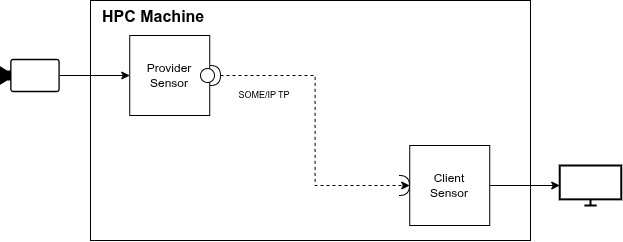
\includegraphics[width=0.75\textwidth]{Images/chapter4/archDesign.png}
%     \vspace{0.5cm}
%     \caption{The architecture design of prototype project}
%     \label{fig:archDesign_project}
% \end{figure}

% Figure~\ref{fig:archDesign_project} illustrates the overall architecture of the prototype system deployed on a High-Performance Computing (HPC) machine. The design follows the Adaptive AUTOSAR methodology, in which software functionalities are decomposed into independent applications that communicate through well-defined service interfaces. In the proposed prototype, the system is organized around two main applications, namely the Provider Sensor and the Client Sensor, which interact through SOME/IP with transport protocol (SOME/IP-TP).

% The Provider Sensor is responsible for collecting, decoding, and processing sensor-related input data, as well as providing processed information to other applications in the system. It acts as a data provider within the service-oriented architecture, exposing its services to subscribed clients. The Client Sensor consumes the provided data, performs perception and decision-related tasks, and generates user-facing outputs such as warnings or visualization results. This clear separation of responsibilities improves modularity and reflects typical ADAS software design principles.

% The prototype focuses on validating both functional correctness and system integration aspects rather than achieving production-level optimization. All applications are executed within a controlled Adaptive AUTOSAR runtime environment, enabling evaluation of inter-application communication, execution flow, and end-to-end behavior. The following subsections describe the implementation details of each component and present the experimental results obtained from the prototype evaluation.

% \chapter{Provider Sensor}
% 

% \chapter{Flow Chart}
% \begin{figure}[H]
% \centering
% \begin{tikzpicture}[
%     node distance=1.5cm,
%     every node/.style={font=\small},
%     startstop/.style={
%         rectangle, rounded corners,
%         minimum width=3.6cm,
%         minimum height=0.9cm,
%         draw, align=center
%     },
%     process/.style={
%         rectangle,
%         minimum width=4.4cm,
%         minimum height=0.9cm,
%         draw, align=center
%     },
%     decision/.style={
%         diamond,
%         aspect=2.8,
%         minimum width=2.6cm,
%         minimum height=0.85cm,
%         inner sep=1.5pt,
%         draw, align=center
%     },
%     arrow/.style={->, thick},
% ]

% % ===== Nodes =====
% \node (start) [startstop] {Application Start};

% \node (init) [process, below of=start] {Initialize ProviderSensor};

% \node (tflite) [process, below of=init] {Initialize TFLite Model};

% \node (checkinit) [decision, below of=tflite, yshift=-0.5cm]
% {Initialization Successful};

% \node (terminate) [startstop, right=3.8cm of checkinit]
% {Terminate Application};

% \node (startport) [process, below of=checkinit, yshift=-0.4cm]
% {Start Sensorv2 Port};

% \node (run) [process, below of=startport]
% {Run Application Thread};

% \node (caminit) [process, below of=run]
% {Open Camera Device};

% \node (camcheck) [decision, below of=caminit, yshift=-0.5cm]
% {Camera Opened};

% \node (cont) [startstop, below of=camcheck, yshift=-0.4cm]
% {Enter Main Processing Loop};

% % ===== Arrows =====
% \draw [arrow] (start) -- (init);
% \draw [arrow] (init) -- (tflite);
% \draw [arrow] (tflite) -- (checkinit);

% \draw [arrow] (checkinit) -- node[right]{Yes} (startport);
% \draw [arrow] (checkinit.east) -- node[above]{No} (terminate.west);

% \draw [arrow] (startport) -- (run);
% \draw [arrow] (run) -- (caminit);
% \draw [arrow] (caminit) -- (camcheck);

% \draw [arrow] (camcheck) -- node[right]{Yes} (cont);
% \draw [arrow]
%     (camcheck.east)
%     -| node[near start, above]{No}
%     (terminate.south);

% \end{tikzpicture}
% \vspace{0.5cm}
% \caption{Initialization Flow of the ProviderSensor Adaptive Application}
% \label{fig:providersensor_init}
% \end{figure}

% \begin{figure}[H]
% \centering
% \begin{tikzpicture}[
%     node distance=1.4cm,
%     every node/.style={font=\small},
%     startstop/.style={
%         rectangle, rounded corners,
%         minimum width=3.6cm,
%         minimum height=0.9cm,
%         draw, align=center
%     },
%     process/.style={
%         rectangle,
%         minimum width=4.6cm,
%         minimum height=0.9cm,
%         draw, align=center
%     },
%     decision/.style={
%         diamond,
%         aspect=2.6,
%         minimum width=3.2cm,
%         minimum height=1.0cm,
%         inner sep=1.5pt,
%         draw, align=center
%     },
%     arrow/.style={->, thick}
% ]

% % ===== Nodes =====
% \node (loop) [startstop] {Main Processing Loop};

% \node (capture) [process, below of=loop]
% {Capture Camera Frame};

% \node (frameok) [decision, below of=capture]
% {Frame Valid};

% \node (infer) [process, below of=frameok, yshift=-0.4cm]
% {YOLO TFLite Inference};

% \node (post) [process, below of=infer]
% {Post Processing\\ Confidence Filter and NMS};

% \node (drawbox) [process, below of=post]
% {Draw Bounding Boxes};

% \node (encode) [process, below of=drawbox]
% {Encode Frame to JPEG};

% \node (send) [process, below of=encode]
% {Send Data via Sensorv2 Port};

% \node (sleep) [process, below of=send]
% {Sleep to Control Frame Rate};

% % ===== Arrows =====
% \draw [arrow] (loop) -- (capture);
% \draw [arrow] (capture) -- (frameok);

% % Decision: Frame Valid
% \draw [arrow] (frameok) -- node[right]{Yes} (infer);
% \draw [arrow]
%     (frameok.east) -- ++(2.2cm,0)
%     |- node[near start, above]{No} (capture.east);

% % Main pipeline
% \draw [arrow] (infer) -- (post);
% \draw [arrow] (post) -- (drawbox);
% \draw [arrow] (drawbox) -- (encode);
% \draw [arrow] (encode) -- (send);
% \draw [arrow] (send) -- (sleep);

% % Loop back
% \draw [arrow]
%     (sleep.west) -- ++(-2.6cm,0)
%     |- (loop.west);

% \end{tikzpicture}
% \vspace{0.5cm}
% \caption{Runtime Processing Loop of the ProviderSensor Application}
% \label{fig:providersensor_runtime}
% \end{figure}

% The process begins with the application startup, followed immediately by the initialization of the \texttt{ProviderSensor} component and the TensorFlow Lite (TFLite) model. The system then verifies if the initialization was successful. If the initialization fails, the application terminates immediately. Upon success, the system starts the \texttt{Sensorv2} communication port and launches the application thread. The flow proceeds to open the camera device. A check is performed to confirm if the camera opened successfully; if not, the application terminates. If the camera is successfully accessed, the system transitions into the main processing loop.

% Once inside the main processing loop, the system continuously captures camera frames. For each iteration, it verifies if the captured frame is valid. If the frame is invalid, the loop restarts. If valid, the system performs inference using the YOLO TFLite model, followed by post-processing steps which include applying a confidence filter and Non-Maximum Suppression (NMS) to refine detections. The system then draws bounding boxes around detected objects and encodes the frame into JPEG format. This processed data is sent via the \texttt{Sensorv2} port. Finally, the loop includes a sleep interval to control the frame rate before repeating the process.




% \chapter{Flow Chart}
\begin{figure}[H]
\centering
\begin{tikzpicture}[
    scale=0.9, transform shape,
    node distance=1.5cm,
    every node/.style={font=\small},
    startstop/.style={
        rectangle, rounded corners,
        minimum width=3.6cm,
        minimum height=0.9cm,
        draw, align=center
    },
    process/.style={
        rectangle,
        minimum width=4.4cm,
        minimum height=0.9cm,
        draw, align=center
    },
    io/.style={
        trapezium, trapezium left angle=70, trapezium right angle=110,
        minimum width=4.0cm, minimum height=0.9cm,
        inner xsep=0.5cm,
        draw, align=center
    },
    decision/.style={
        diamond,
        aspect=2.8,
        minimum width=2.6cm,
        minimum height=0.85cm,
        inner sep=1.5pt,
        draw, align=center
    },
    arrow/.style={->, thick},
]

% ===== Nodes =====
\node (start) [startstop] {Application Start};

\node (init) [process, below of=start] {Initialize Provider Application};

\node (caminit) [process, below of=init] {Open UART (GPS) \& USB (Webcam)};

\node (checkinit) [decision, below of=caminit, yshift=-0.5cm]
{Devices Opened?};

\node (terminate) [startstop, right=3.8cm of checkinit]
{Terminate Application};

\node (startdds) [process, below of=checkinit, yshift=-0.4cm]
{Initialize DDS Publisher\\Service: \texttt{Sensor}, ID: \texttt{100}};

\node (loop) [startstop, below of=startdds]
{Main Processing Loop};

\node (capture) [io, below of=loop]
{1. Data Acquisition (GPS \& Frame)};

\node (yolo) [process, below of=capture]
{2a. YOLO Traffic Light Detection};

% Multi-thread fork (One thread per Direction)
\node (fork) [rectangle, fill=black, inner sep=0pt, minimum width=8.5cm, minimum height=0.15cm, below of=yolo, yshift=-0.2cm] {};

\node (t1) [process, minimum width=3.6cm, align=center, below of=fork, xshift=-2.8cm, yshift=-0.4cm]
{\textbf{Thread 1 (e.g., Left)}\\Extract ROI\\HSV Color Pipeline\\Timer Detection};

\node (tn) [process, minimum width=3.6cm, align=center, below of=fork, xshift=2.8cm, yshift=-0.4cm]
{\textbf{Thread 3 (e.g., Straight)}\\Extract ROI\\HSV Color Pipeline\\Timer Detection};

\node (dots) [below of=fork, yshift=-1.9cm] {\Large $\dots$};

% Multi-thread join
\node (join) [rectangle, fill=black, inner sep=0pt, minimum width=8.5cm, minimum height=0.15cm, below of=t1, xshift=2.8cm, yshift=-0.8cm] {};

\node (pack) [process, below of=join, yshift=0.3cm]
{3. Pack \texttt{GpsJpegWireHeader} + JPEG};

\node (publish) [io, below of=pack]
{4. Publish \texttt{imageDataEvent}\\Topic: \texttt{imageData}};

% ===== Arrows =====
\draw [arrow] (start) -- (init);
\draw [arrow] (init) -- (caminit);
\draw [arrow] (caminit) -- (checkinit);

\draw [arrow] (checkinit) -- node[right]{Yes} (startdds);
\draw [arrow] (checkinit.east) -- node[above]{No} (terminate.west);

\draw [arrow] (startdds) -- (loop);
\draw [arrow] (loop) -- (capture);
\draw [arrow] (capture) -- (yolo);

\draw [arrow] (yolo) -- (fork);
\draw [arrow] (t1.north |- fork.south) -- (t1.north);
\draw [arrow] (tn.north |- fork.south) -- (tn.north);

\draw [arrow] (t1.south) -- (t1.south |- join.north);
\draw [arrow] (tn.south) -- (tn.south |- join.north);
\draw [arrow] (join.south) -- (pack.north);

\draw [arrow] (pack) -- (publish);

% Loop back
\draw [arrow]
    (publish.west) -- ++(-3.8cm,0)
    |- (loop.west);

\end{tikzpicture}
\vspace{0.5cm}
\caption{Processing Flow of the Provider Application}
\label{fig:provider_flow}
\end{figure}

The application initiates the Provider component by acquiring access to the necessary external peripherals: the GPS module via UART (\texttt{/dev/ttyAMA0}) and the external webcam via USB 2.0 (UVC). Upon successful hardware initialization, the application establishes the DDS Publisher node configured for the \texttt{Sensor} service (instance-id~\texttt{100}, Domain Id~\texttt{0}) using the \texttt{CycloneDDS-CXX} stack over UDP. Failure at either the hardware or network initialization stage results in an immediate application termination to ensure system safety.

Once the setup is complete, the execution enters the main processing loop where data acquisition and perception tasks operate continuously. The pipeline captures a raw video frame from the webcam simultaneously with the reading of GPS position data. The raw frame is passed to the YOLO-based Traffic Light Detection module to infer initial bounding boxes. To meet real-time constraints, the subsequent processing stages are parallelized. The algorithm selects the highest-confidence bounding box for each distinct traffic light direction (Left, Right, Straight) and dispatches a dedicated worker thread for each direction. The concurrent operations within these threads are detailed in Figure~\ref{fig:thread_flow}.

\begin{figure}[H]
\centering
\begin{tikzpicture}[
    scale=0.9, transform shape,
    node distance=1.4cm,
    every node/.style={font=\small},
    startstop/.style={
        rectangle, rounded corners,
        minimum width=3.6cm,
        minimum height=0.9cm,
        draw, align=center
    },
    process/.style={
        rectangle,
        minimum width=4.8cm,
        minimum height=0.9cm,
        draw, align=center
    },
    decision/.style={
        diamond,
        aspect=2.8,
        minimum width=3.0cm,
        minimum height=1.0cm,
        inner sep=1.5pt,
        draw, align=center
    },
    arrow/.style={->, thick},
]

% Nodes
\node (start) [startstop] {Thread Start (dirWorker)};

\node (extract_tl) [process, below of=start] {Extract Traffic Light ROI\\on Original High-Res Image};

\node (hsv) [process, below of=extract_tl] {HSV Color Classification};

\node (check_timer) [decision, below of=hsv, yshift=-0.5cm] {Timer Boxes\\Detected?};

\node (find_nearest) [process, below of=check_timer, yshift=-0.5cm] {Find Nearest Timer Box\\(Distance Calculation)};

\node (check_nearest) [decision, below of=find_nearest, yshift=-0.5cm] {Valid Timer\\Box Found?};

\node (extract_timer) [process, below of=check_nearest, yshift=-0.5cm] {Extract Timer ROI\\on Original High-Res Image};

\node (ocr) [process, below of=extract_timer] {Lightweight OCR Model\\(Digit Recognition)};

\node (end) [startstop, right=3.5cm of check_nearest] {Return Direction\\Result};

% Arrows
\draw [arrow] (start) -- (extract_tl);
\draw [arrow] (extract_tl) -- (hsv);
\draw [arrow] (hsv) -- (check_timer);

\draw [arrow] (check_timer) -- node[right]{Yes} (find_nearest);
\draw [arrow] (check_timer.east) -| node[near start, above]{No} (end.north);

\draw [arrow] (find_nearest) -- (check_nearest);
\draw [arrow] (check_nearest) -- node[above]{No} (end.west);
\draw [arrow] (check_nearest) -- node[right]{Yes} (extract_timer);

\draw [arrow] (extract_timer) -- (ocr);
\draw [arrow] (ocr.east) -| (end.south);

\end{tikzpicture}
\vspace{0.5cm}
\caption{Parallel Thread Pipeline for each Direction (dirWorker)}
\label{fig:thread_flow}
\end{figure}

Within each direction's worker thread (\texttt{dirWorker}), the pipeline maps the low-resolution YOLO bounding box back to the original high-resolution frame to extract a precise Region of Interest (ROI). This ROI undergoes an HSV color space transformation to robustly classify the current signal state. Concurrently, the thread identifies any timer boxes detected in the main frame. By calculating geometric distances, the algorithm pairs the nearest valid timer box with the corresponding traffic light direction. If a match is found, the timer's ROI is extracted from the high-resolution frame and passed through a lightweight OCR model to recognize the remaining countdown digits.

Upon the completion of all parallel threads, the main thread synchronizes the multi-directional results. The annotated frame is then JPEG-encoded and serialized alongside a 24-byte \texttt{GpsJpegWireHeader}. This custom header encapsulates the metadata, including the magic value, protocol version, \texttt{in\_range} flag, \texttt{node\_id}, \texttt{dist\_m}, and the payload length (\texttt{jpeg\_len}). Finally, the combined byte sequence is written into the \texttt{imageData} payload of the \texttt{dds::sensorCam::imageDataEventType} structure and published over the DDS network to any subscribed clients.


% \chapter{Client Sensor}
% % \chapter{Flow Chart}

% \begin{figure}[H]
% \centering
% \begin{tikzpicture}[
%     node distance=1.4cm,
%     every node/.style={font=\small},
%     startstop/.style={
%         rectangle, rounded corners,
%         minimum width=3.8cm,
%         minimum height=0.9cm,
%         draw, align=center
%     },
%     process/.style={
%         rectangle,
%         minimum width=4.8cm,
%         minimum height=0.9cm,
%         draw, align=center
%     },
%     decision/.style={
%         diamond,
%         aspect=2.6,
%         minimum width=3.6cm,
%         minimum height=1.1cm,
%         inner sep=1.5pt,
%         draw, align=center
%     },
%     arrow/.style={->, thick}
% ]

% % ===== Nodes =====
% \node (start) [startstop] {Application Start};

% \node (init) [process, below of=start]
% {Initialize ClientSensor};

% \node (register) [process, below of=init]
% {Register Sensorv2\\ Event Handler};

% \node (startport) [process, below of=register]
% {Start Sensorv2 Port};

% \node (wait) [process, below of=startport]
% {Wait for Incoming Data Event};

% \node (dataok) [decision, below of=wait]
% {Data Received};

% \node (decode) [process, below of=dataok, yshift=-0.4cm]
% {Decode JPEG Data};

% \node (decodeok) [decision, below of=decode]
% {Decode Successful};

% \node (save) [process, below of=decodeok, yshift=-0.4cm]
% {Save Image to File};

% \node (saveok) [decision, below of=save]
% {Save Successful};

% \node (logerr) [process, right=4.6cm of decodeok]
% {Log Error};

% % ===== Main Flow =====
% \draw [arrow] (start) -- (init);
% \draw [arrow] (init) -- (register);
% \draw [arrow] (register) -- (startport);
% \draw [arrow] (startport) -- (wait);
% \draw [arrow] (wait) -- (dataok);

% % Data received decision
% \draw [arrow] (dataok) -- node[right]{Yes} (decode);
% \draw [arrow] (dataok.west) -- ++(-1cm,0) |- node[near start, above]{No} (wait.west);

% % Decode path
% \draw [arrow] (decode) -- (decodeok);

% \draw [arrow] (decodeok) -- node[right]{Yes} (save);
% \draw [arrow] (decodeok.east) -- node[near start, above]{No} (logerr.west);

% % Save decision
% \draw [arrow] (save) -- (saveok);

% \draw [arrow]
%     (saveok.west)
%     -- ++(-1.6cm,0)
%     |- node[near start, above]{Yes}
%     (wait.west);
    
% \draw [arrow] (saveok.east) -| node[near start, above]{No} (logerr.south);

% % Error loop back
% \draw [arrow] (logerr.north) |- (wait.east);


% \end{tikzpicture}

% \vspace{0.5cm}
% \caption{ClientSensor Data Reception and Processing Flow}
% \label{fig:clientsensor_flow}
% \end{figure}

% Data Reception and Processing Flow The Client Sensor workflow starts with the application launch and the initialization of the \texttt{ClientSensor} unit. The system registers the \texttt{Sensorv2} event handler and starts the \texttt{Sensorv2} port to enable communication. It then enters a standby state to wait for incoming data events. When data is received, the system attempts to decode the incoming JPEG data. A decision block checks if the decoding was successful; if not, an error is logged. If decoding succeeds, the system proceeds to save the image to a file. A final check confirms if the file save was successful. If the save operation fails, an error is logged; otherwise, the data handling for that event is considered complete.


% \subsection{Flow Chart}

\begin{figure}[H]
\centering
\begin{tikzpicture}[
    node distance=1.4cm,
    every node/.style={font=\small},
    startstop/.style={
        rectangle, rounded corners,
        minimum width=3.8cm,
        minimum height=0.9cm,
        draw, align=center
    },
    process/.style={
        rectangle,
        minimum width=4.8cm,
        minimum height=0.9cm,
        draw, align=center
    },
    decision/.style={
        diamond,
        aspect=2.6,
        minimum width=3.6cm,
        minimum height=1.1cm,
        inner sep=1.5pt,
        draw, align=center
    },
    arrow/.style={->, thick}
]

% ===== Nodes =====
\node (start) [startstop] {Application Start};

\node (init) [process, below of=start]
{Initialize Client Application};

\node (sub) [process, below of=init]
{1. Subscribe \texttt{imageDataEvent}\\Topic: \texttt{imageData}};

\node (wait) [process, below of=sub]
{Wait for \texttt{imageDataEvent}};

\node (dataok) [decision, below of=wait]
{Event Received};

\node (parse) [process, below of=dataok, yshift=-0.4cm]
{2. Parse \texttt{GpsJpegWireHeader} + JPEG};

\node (tcp) [process, below of=parse]
{3. TCP Client\\\texttt{127.0.0.1:8888}};

\node (sendok) [decision, below of=tcp, yshift=-0.4cm]
{Transmission Successful};

\node (out) [process, below of=sendok, yshift=-0.4cm]
{4. Output to External Display};

\node (logerr) [process, right=4.6cm of dataok]
{Log Error};

% ===== Main Flow =====
\draw [arrow] (start) -- (init);
\draw [arrow] (init) -- (sub);
\draw [arrow] (sub) -- (wait);
\draw [arrow] (wait) -- (dataok);

% Data received decision
\draw [arrow] (dataok) -- node[right]{Yes} (parse);
\draw [arrow] (dataok.west) -- ++(-1cm,0) |- node[near start, above]{No} (wait.west);

% Decode path
\draw [arrow] (parse) -- (tcp);
\draw [arrow] (tcp) -- (sendok);

\draw [arrow] (sendok) -- node[right]{Yes} (out);
\draw [arrow] (sendok.east) -| node[near start, above]{No} (logerr.south);

% Loop back
\draw [arrow]
    (out.west)
    -- ++(-1.6cm,0)
    |-
    (wait.west);
    
% Error loop back
\draw [arrow] (logerr.north) |- (wait.east);

\end{tikzpicture}

\vspace{0.5cm}
\caption{Client Data Reception and Processing Flow}
\label{fig:client_flow}
\end{figure}

Upon startup, the Client application initializes its DDS Subscriber node. It registers a listener for the \texttt{imageDataEvent} on the \texttt{imageData} topic, targeting the \texttt{Sensor} service. The application is configured to discover any available provider (instance-id~\texttt{ANY}) operating on Domain Id~\texttt{0}. Once the DDS entities are established via the \texttt{CycloneDDS-CXX} middleware, the subscriber thread blocks and waits for incoming \texttt{dds::sensorCam::imageDataEventType} messages.

Upon receiving an event, the application extracts the \texttt{imageData} payload and decodes its byte structure. The parser reads the initial 24 bytes to reconstruct the \texttt{GpsJpegWireHeader}, extracting vital metadata such as the \texttt{in\_range} flag, \texttt{node\_id}, \texttt{dist\_m}, and \texttt{jpeg\_len}. Subsequently, it extracts the JPEG image bytes corresponding to the \texttt{jpeg\_len} field. 

To bridge the DDS middleware with the user-facing interface, the Client acts as a TCP proxy. It marshals the decoded data into a custom TCP packet structured as \texttt{[uint32 frame\_len][JPEG][uint8 in\_range][int64 node\_id][int32 dist\_m]} and transmits it to the external display monitor listening at \texttt{127.0.0.1:8888}. In case of a socket error, the application logs the failure and attempts reconnection. Otherwise, the HMI updates the visualization with the latest camera frame and GPS metadata, and the subscriber returns to its listening state for the next DDS event.

% \chapter{Result}
% % \begin{figure}[H]
%     \centering
%     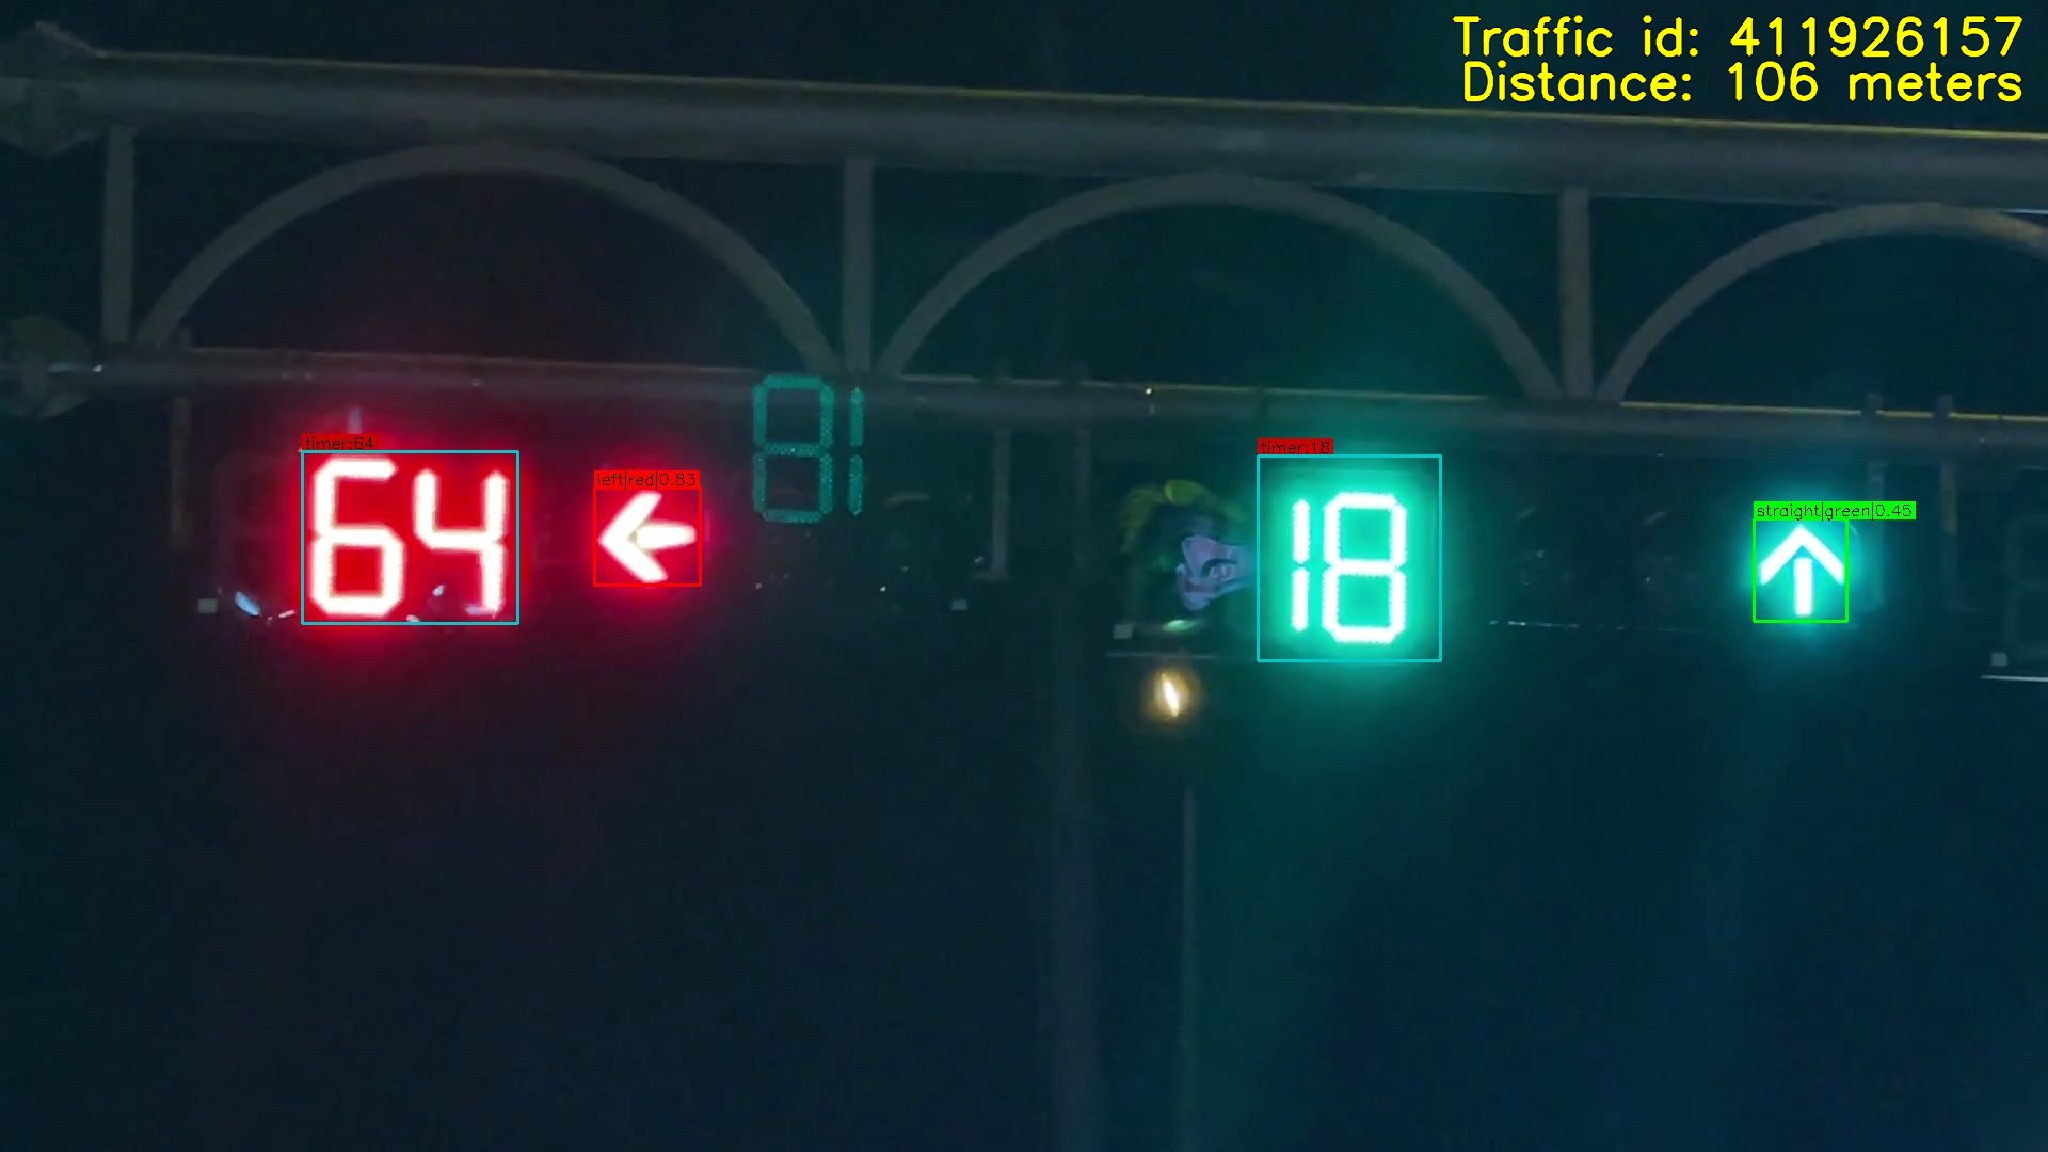
\includegraphics[width=0.75\textwidth]{Images/chapter4/result.png}
%     \vspace{0.5cm}
%     \caption{The result of prototype project}
%     \label{fig:res_project}
% \end{figure}

% Figure~\ref{fig:res_project} illustrates the experimental result obtained from the implemented prototype system. The figure shows the output generated by the ClientSensor application after receiving processed data from the ProviderSensor through the Adaptive AUTOSAR communication mechanism.

% In this experiment, the ClientSensor performs camera-based traffic light detection using the trained YOLO-MobileNet model. Detected traffic lights are highlighted with bounding boxes, and each detection is annotated with the corresponding class label and confidence score, such as red, yellow, and green signal states. The visualization demonstrates that the system is capable of identifying multiple traffic light instances within a single frame and distinguishing different signal colors under indoor test conditions.

% The execution logs displayed in the terminal confirm the end-to-end data flow within the Adaptive AUTOSAR environment. The ProviderSensor successfully publishes processed sensor data, which is then received and consumed by the ClientSensor via SOME/IP with transport protocol (SOME/IP-TP). The logs indicate correct service discovery, data transmission, and event handling between the two applications. Furthermore, the generated output image is stored locally, verifying that the perception results are correctly transferred and processed at the application level.

% Overall, this result validates the functional correctness of the prototype, demonstrating successful integration of deep learning–based perception with Adaptive AUTOSAR service-oriented communication. While the experiment is conducted in a controlled environment and does not represent full automotive deployment conditions, it confirms the feasibility of the proposed architecture and provides a solid foundation for further system optimization and real-world validation.

\subsection{Experimental Setup}
To evaluate the end-to-end functionality of the proposed ADAS architecture followed by the Figure~\ref{fig:archDesign_project}, a hardware-in-the-loop (HIL) experiment was conducted, as previously illustrated in Figure~\ref{fig:hw_arch} in Chapter 2. The setup was designed to simulate a practical in-vehicle network. Specifically, a Raspberry Pi 5 was utilized as the edge computing node to run the Provider application, which handles heavy tasks such as model inference and sensor data collection. A standard USB UVC webcam was connected to capture real-time video streams, while a GPS module supplied accurate vehicle positioning data via a UART interface.
To create a realistic distributed environment, the Client application and the visualization Human-Machine Interface (HMI) were hosted on a separate monitoring computer. This machine was connected to the Raspberry Pi 5 over a Local Area Network (LAN). This separation is important because it ensures that the edge node's processing power is dedicated entirely to AI inference, rather than displaying graphics. 

Furthermore, the overall effectiveness of this setup relies on well-trained perception models. The specific datasets and training configurations used to develop the YOLO26-MobileNetV4 model and the lightweight multi-head CNN timer detector are discussed in detail in Section~\ref{sub:datasetYolo} and Section~\ref{sec:dataCNN}, respectively.

\subsection{System Evaluation}
\begin{figure}[H]
    \centering
    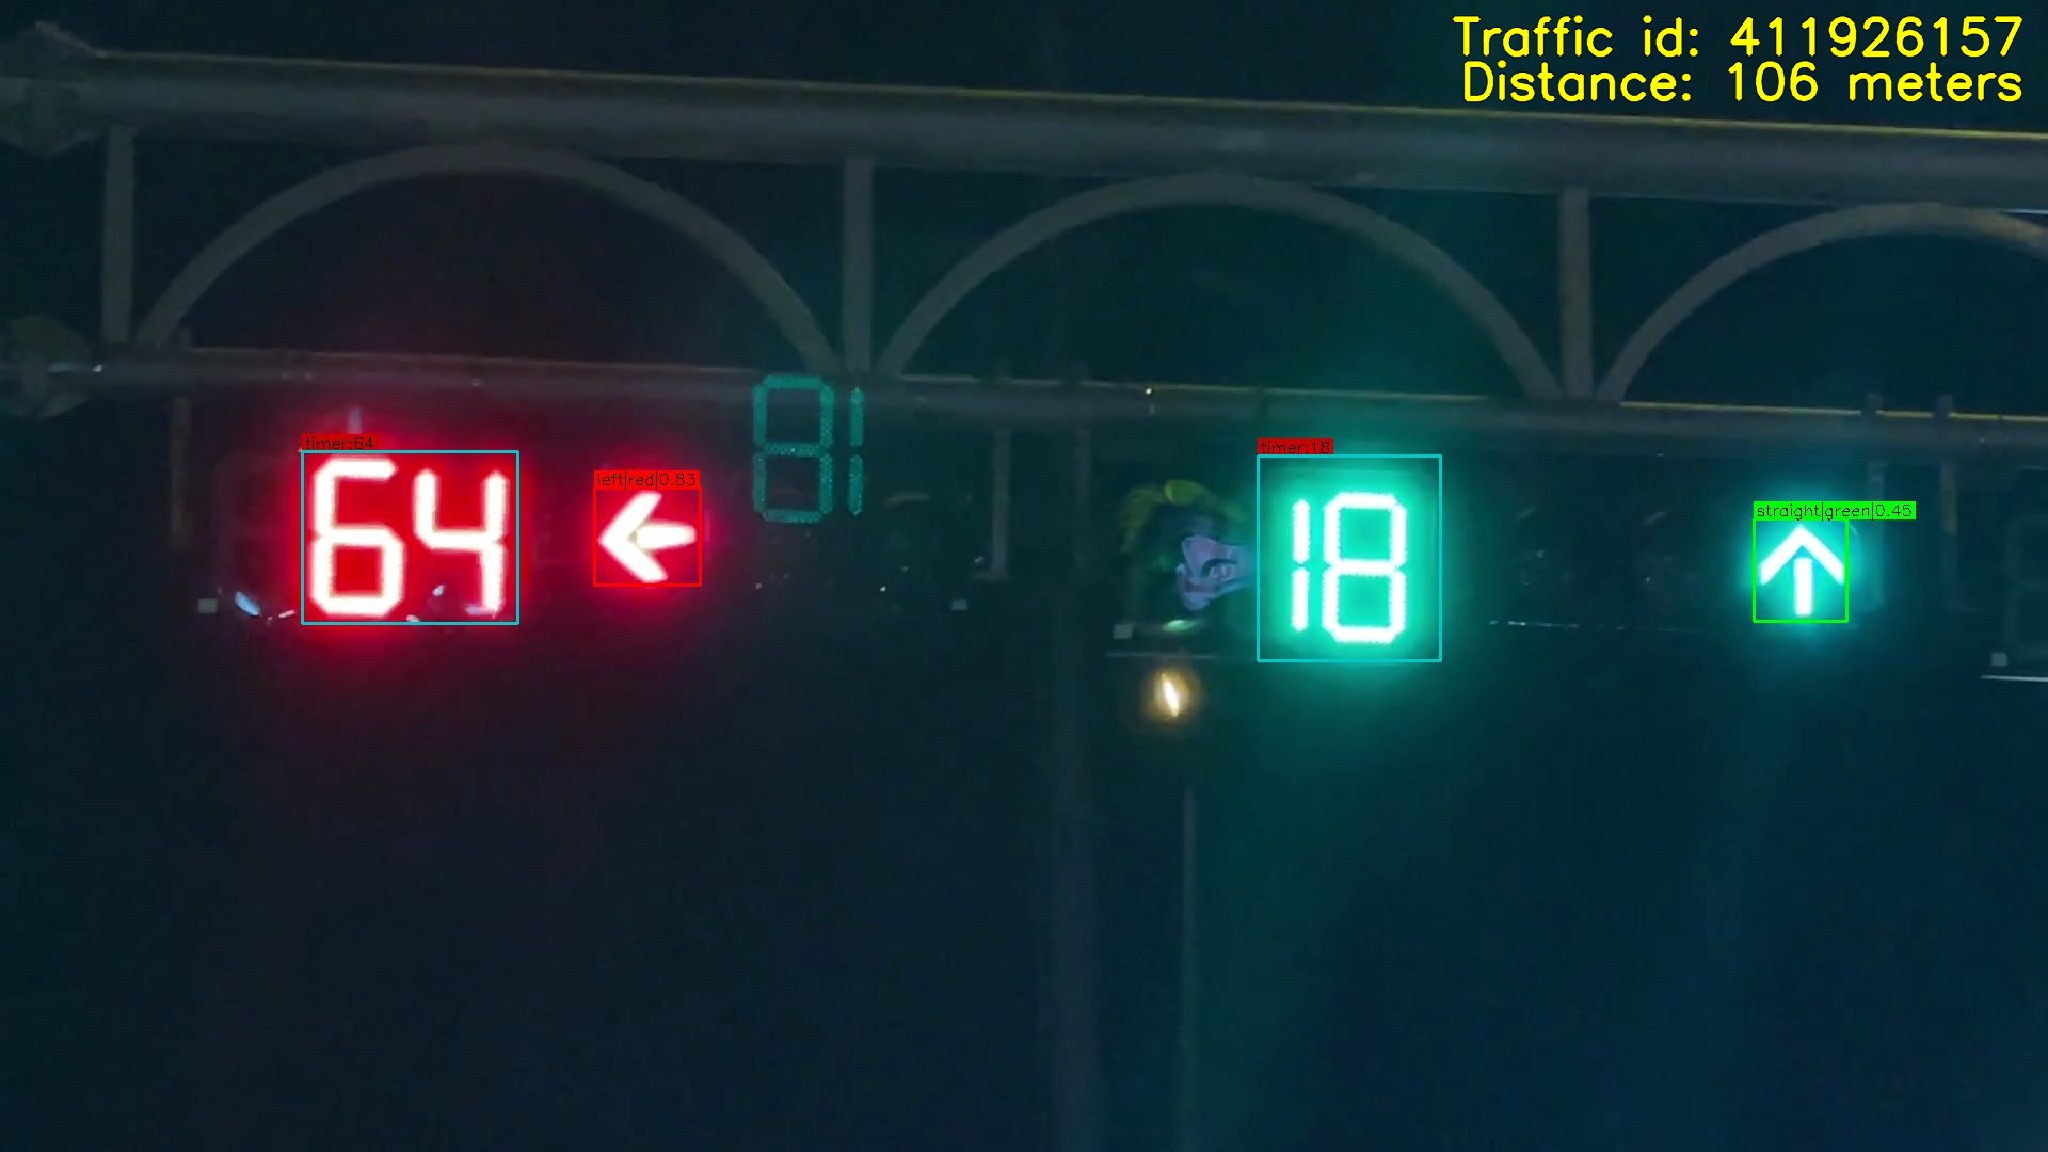
\includegraphics[width=0.75\textwidth]{Images/chapter4/result.png}
    \vspace{0.5cm}
    \caption{Prototype output displayed by the HMI/monitor}
    \label{fig:res_project}
\end{figure}

Figure~\ref{fig:res_project} presents the final visualization produced by the prototype. The monitoring HMI successfully received the data stream from the Client application over the TCP connection. The overlay in the upper-right corner reflects the traffic-light node metadata extracted from the DDS payload, correctly identifying \texttt{Traffic id: 411926157} at a \texttt{Distance: 106 meters}.

During execution, the Provider's perception pipeline successfully captured the camera frame, recognized the traffic light states, and annotated the image. The output highlights a red right-turn signal with a countdown of \texttt{64} seconds and a green straight signal with \texttt{18} seconds remaining. The seamless presentation of both the annotated image and the corresponding GPS metadata confirms that the \texttt{GpsJpegWireHeader} parsing logic functions correctly on the Client side. 

Furthermore, the successful display verifies the reliability of the underlying communication architecture. The \texttt{CycloneDDS-CXX} middleware managed the service discovery and the transportation of the \texttt{imageDataEvent} without observable payload corruption. The experiment demonstrates that the combination of edge-based perception, DDS-driven data distribution, and TCP-based visualization can sustain the required data flow for an ADAS prototype without relying on generic system boilerplates.

With the technical implementations and methodological frameworks thoroughly detailed and validated in Chapter 4, the primary objectives of this research have been addressed. Transitioning into Chapter 5, the focus will shift towards a final synthesis of the project. The upcoming chapter will offer a conclusive summary of the findings, reflect on the practical implications of the developed ADAS system, and propose viable recommendations for future enhancements.


\chapter{Project Prototype}

This chapter presents the implementation of the proposed red-light warning prototype. Inspired by the traffic light recognition approach combining a monocular camera with intelligent transport system data~\cite{Lee2022TrafficLightRecognition}, this prototype utilizes GPS coordinates to calculate the vehicle's distance to the nearest traffic-light node. Upon entering a predefined warning zone, the camera-based perception pipeline is triggered to identify the traffic light direction, classify the signal state, and extract the countdown timer. The processed data is then transmitted to the user display interface.

\begin{figure}[H]
    \centering
    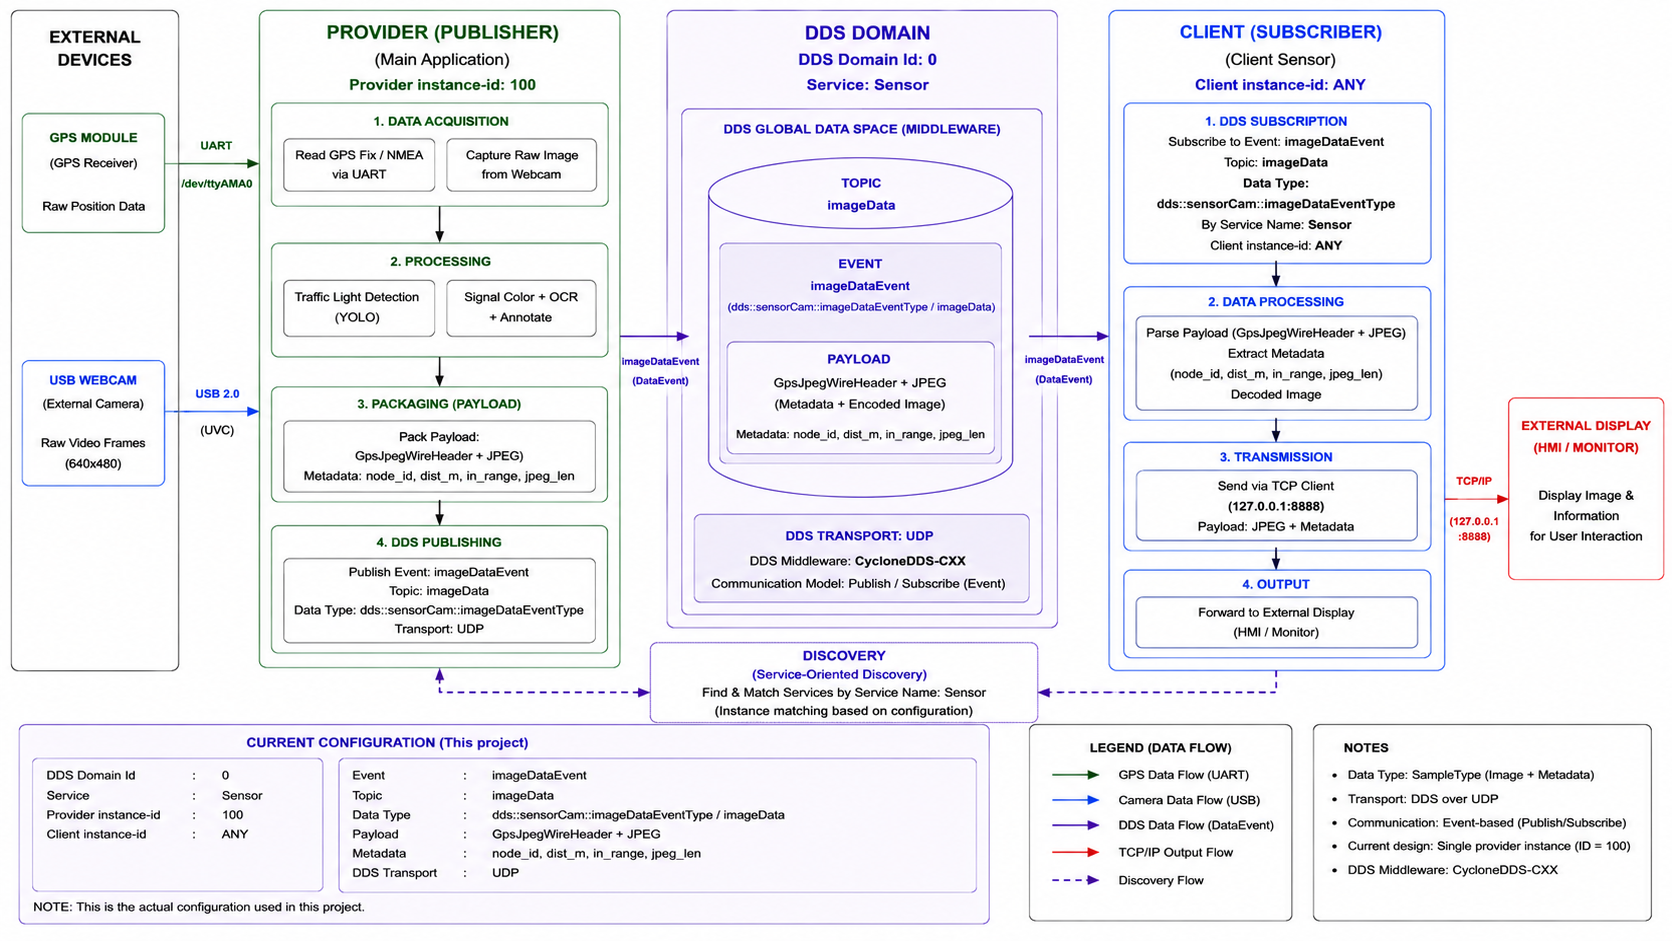
\includegraphics[width=1\textwidth]{Images/chapter4/architecture.png}
    \vspace{0.5cm}
    \caption{The architecture design of prototype project}
    \label{fig:archDesign_project}
\end{figure}

Figure~\ref{fig:archDesign_project} illustrates the architecture of the prototype deployed on a Raspberry Pi 5. The design adopts a service-oriented approach, where functionalities are decoupled into distinct applications communicating via the DDS (Data Distribution Service) middleware (\texttt{CycloneDDS-CXX}).

The architecture comprises two main components:
\begin{itemize}
    \item \textbf{Provider (Main Application):} Handles data acquisition from the GPS module and USB webcam. It executes the deep learning pipeline (YOLO detection, color classification, and OCR), encodes the output into a \texttt{GpsJpegWireHeader} along with JPEG bytes, and publishes the payload as a DDS event.
    \item \textbf{Client (Client Sensor):} Subscribes to the DDS event, parses the payload, and forwards the reconstructed JPEG and metadata over a TCP connection to an external HMI/Monitor for visualization.
\end{itemize}

This separation of concerns allows for independent deployment and testing of perception and visualization tasks. The specific implementation workflows for the Provider and Client are detailed in the following subsections.

\section{Provider Sensor (Publisher)}


% \chapter{Flow Chart}
% \begin{figure}[H]
% \centering
% \begin{tikzpicture}[
%     node distance=1.5cm,
%     every node/.style={font=\small},
%     startstop/.style={
%         rectangle, rounded corners,
%         minimum width=3.6cm,
%         minimum height=0.9cm,
%         draw, align=center
%     },
%     process/.style={
%         rectangle,
%         minimum width=4.4cm,
%         minimum height=0.9cm,
%         draw, align=center
%     },
%     decision/.style={
%         diamond,
%         aspect=2.8,
%         minimum width=2.6cm,
%         minimum height=0.85cm,
%         inner sep=1.5pt,
%         draw, align=center
%     },
%     arrow/.style={->, thick},
% ]

% % ===== Nodes =====
% \node (start) [startstop] {Application Start};

% \node (init) [process, below of=start] {Initialize ProviderSensor};

% \node (tflite) [process, below of=init] {Initialize TFLite Model};

% \node (checkinit) [decision, below of=tflite, yshift=-0.5cm]
% {Initialization Successful};

% \node (terminate) [startstop, right=3.8cm of checkinit]
% {Terminate Application};

% \node (startport) [process, below of=checkinit, yshift=-0.4cm]
% {Start Sensorv2 Port};

% \node (run) [process, below of=startport]
% {Run Application Thread};

% \node (caminit) [process, below of=run]
% {Open Camera Device};

% \node (camcheck) [decision, below of=caminit, yshift=-0.5cm]
% {Camera Opened};

% \node (cont) [startstop, below of=camcheck, yshift=-0.4cm]
% {Enter Main Processing Loop};

% % ===== Arrows =====
% \draw [arrow] (start) -- (init);
% \draw [arrow] (init) -- (tflite);
% \draw [arrow] (tflite) -- (checkinit);

% \draw [arrow] (checkinit) -- node[right]{Yes} (startport);
% \draw [arrow] (checkinit.east) -- node[above]{No} (terminate.west);

% \draw [arrow] (startport) -- (run);
% \draw [arrow] (run) -- (caminit);
% \draw [arrow] (caminit) -- (camcheck);

% \draw [arrow] (camcheck) -- node[right]{Yes} (cont);
% \draw [arrow]
%     (camcheck.east)
%     -| node[near start, above]{No}
%     (terminate.south);

% \end{tikzpicture}
% \vspace{0.5cm}
% \caption{Initialization Flow of the ProviderSensor Adaptive Application}
% \label{fig:providersensor_init}
% \end{figure}

% \begin{figure}[H]
% \centering
% \begin{tikzpicture}[
%     node distance=1.4cm,
%     every node/.style={font=\small},
%     startstop/.style={
%         rectangle, rounded corners,
%         minimum width=3.6cm,
%         minimum height=0.9cm,
%         draw, align=center
%     },
%     process/.style={
%         rectangle,
%         minimum width=4.6cm,
%         minimum height=0.9cm,
%         draw, align=center
%     },
%     decision/.style={
%         diamond,
%         aspect=2.6,
%         minimum width=3.2cm,
%         minimum height=1.0cm,
%         inner sep=1.5pt,
%         draw, align=center
%     },
%     arrow/.style={->, thick}
% ]

% % ===== Nodes =====
% \node (loop) [startstop] {Main Processing Loop};

% \node (capture) [process, below of=loop]
% {Capture Camera Frame};

% \node (frameok) [decision, below of=capture]
% {Frame Valid};

% \node (infer) [process, below of=frameok, yshift=-0.4cm]
% {YOLO TFLite Inference};

% \node (post) [process, below of=infer]
% {Post Processing\\ Confidence Filter and NMS};

% \node (drawbox) [process, below of=post]
% {Draw Bounding Boxes};

% \node (encode) [process, below of=drawbox]
% {Encode Frame to JPEG};

% \node (send) [process, below of=encode]
% {Send Data via Sensorv2 Port};

% \node (sleep) [process, below of=send]
% {Sleep to Control Frame Rate};

% % ===== Arrows =====
% \draw [arrow] (loop) -- (capture);
% \draw [arrow] (capture) -- (frameok);

% % Decision: Frame Valid
% \draw [arrow] (frameok) -- node[right]{Yes} (infer);
% \draw [arrow]
%     (frameok.east) -- ++(2.2cm,0)
%     |- node[near start, above]{No} (capture.east);

% % Main pipeline
% \draw [arrow] (infer) -- (post);
% \draw [arrow] (post) -- (drawbox);
% \draw [arrow] (drawbox) -- (encode);
% \draw [arrow] (encode) -- (send);
% \draw [arrow] (send) -- (sleep);

% % Loop back
% \draw [arrow]
%     (sleep.west) -- ++(-2.6cm,0)
%     |- (loop.west);

% \end{tikzpicture}
% \vspace{0.5cm}
% \caption{Runtime Processing Loop of the ProviderSensor Application}
% \label{fig:providersensor_runtime}
% \end{figure}

% The process begins with the application startup, followed immediately by the initialization of the \texttt{ProviderSensor} component and the TensorFlow Lite (TFLite) model. The system then verifies if the initialization was successful. If the initialization fails, the application terminates immediately. Upon success, the system starts the \texttt{Sensorv2} communication port and launches the application thread. The flow proceeds to open the camera device. A check is performed to confirm if the camera opened successfully; if not, the application terminates. If the camera is successfully accessed, the system transitions into the main processing loop.

% Once inside the main processing loop, the system continuously captures camera frames. For each iteration, it verifies if the captured frame is valid. If the frame is invalid, the loop restarts. If valid, the system performs inference using the YOLO TFLite model, followed by post-processing steps which include applying a confidence filter and Non-Maximum Suppression (NMS) to refine detections. The system then draws bounding boxes around detected objects and encodes the frame into JPEG format. This processed data is sent via the \texttt{Sensorv2} port. Finally, the loop includes a sleep interval to control the frame rate before repeating the process.




% \chapter{Flow Chart}
\begin{figure}[H]
\centering
\begin{tikzpicture}[
    scale=0.9, transform shape,
    node distance=1.5cm,
    every node/.style={font=\small},
    startstop/.style={
        rectangle, rounded corners,
        minimum width=3.6cm,
        minimum height=0.9cm,
        draw, align=center
    },
    process/.style={
        rectangle,
        minimum width=4.4cm,
        minimum height=0.9cm,
        draw, align=center
    },
    io/.style={
        trapezium, trapezium left angle=70, trapezium right angle=110,
        minimum width=4.0cm, minimum height=0.9cm,
        inner xsep=0.5cm,
        draw, align=center
    },
    decision/.style={
        diamond,
        aspect=2.8,
        minimum width=2.6cm,
        minimum height=0.85cm,
        inner sep=1.5pt,
        draw, align=center
    },
    arrow/.style={->, thick},
]

% ===== Nodes =====
\node (start) [startstop] {Application Start};

\node (init) [process, below of=start] {Initialize Provider Application};

\node (caminit) [process, below of=init] {Open UART (GPS) \& USB (Webcam)};

\node (checkinit) [decision, below of=caminit, yshift=-0.5cm]
{Devices Opened?};

\node (terminate) [startstop, right=3.8cm of checkinit]
{Terminate Application};

\node (startdds) [process, below of=checkinit, yshift=-0.4cm]
{Initialize DDS Publisher\\Service: \texttt{Sensor}, ID: \texttt{100}};

\node (loop) [startstop, below of=startdds]
{Main Processing Loop};

\node (capture) [io, below of=loop]
{1. Data Acquisition (GPS \& Frame)};

\node (yolo) [process, below of=capture]
{2a. YOLO Traffic Light Detection};

% Multi-thread fork (One thread per Direction)
\node (fork) [rectangle, fill=black, inner sep=0pt, minimum width=8.5cm, minimum height=0.15cm, below of=yolo, yshift=-0.2cm] {};

\node (t1) [process, minimum width=3.6cm, align=center, below of=fork, xshift=-2.8cm, yshift=-0.4cm]
{\textbf{Thread 1 (e.g., Left)}\\Extract ROI\\HSV Color Pipeline\\Timer Detection};

\node (tn) [process, minimum width=3.6cm, align=center, below of=fork, xshift=2.8cm, yshift=-0.4cm]
{\textbf{Thread 3 (e.g., Straight)}\\Extract ROI\\HSV Color Pipeline\\Timer Detection};

\node (dots) [below of=fork, yshift=-1.9cm] {\Large $\dots$};

% Multi-thread join
\node (join) [rectangle, fill=black, inner sep=0pt, minimum width=8.5cm, minimum height=0.15cm, below of=t1, xshift=2.8cm, yshift=-0.8cm] {};

\node (pack) [process, below of=join, yshift=0.3cm]
{3. Pack \texttt{GpsJpegWireHeader} + JPEG};

\node (publish) [io, below of=pack]
{4. Publish \texttt{imageDataEvent}\\Topic: \texttt{imageData}};

% ===== Arrows =====
\draw [arrow] (start) -- (init);
\draw [arrow] (init) -- (caminit);
\draw [arrow] (caminit) -- (checkinit);

\draw [arrow] (checkinit) -- node[right]{Yes} (startdds);
\draw [arrow] (checkinit.east) -- node[above]{No} (terminate.west);

\draw [arrow] (startdds) -- (loop);
\draw [arrow] (loop) -- (capture);
\draw [arrow] (capture) -- (yolo);

\draw [arrow] (yolo) -- (fork);
\draw [arrow] (t1.north |- fork.south) -- (t1.north);
\draw [arrow] (tn.north |- fork.south) -- (tn.north);

\draw [arrow] (t1.south) -- (t1.south |- join.north);
\draw [arrow] (tn.south) -- (tn.south |- join.north);
\draw [arrow] (join.south) -- (pack.north);

\draw [arrow] (pack) -- (publish);

% Loop back
\draw [arrow]
    (publish.west) -- ++(-3.8cm,0)
    |- (loop.west);

\end{tikzpicture}
\vspace{0.5cm}
\caption{Processing Flow of the Provider Application}
\label{fig:provider_flow}
\end{figure}

The application initiates the Provider component by acquiring access to the necessary external peripherals: the GPS module via UART (\texttt{/dev/ttyAMA0}) and the external webcam via USB 2.0 (UVC). Upon successful hardware initialization, the application establishes the DDS Publisher node configured for the \texttt{Sensor} service (instance-id~\texttt{100}, Domain Id~\texttt{0}) using the \texttt{CycloneDDS-CXX} stack over UDP. Failure at either the hardware or network initialization stage results in an immediate application termination to ensure system safety.

Once the setup is complete, the execution enters the main processing loop where data acquisition and perception tasks operate continuously. The pipeline captures a raw video frame from the webcam simultaneously with the reading of GPS position data. The raw frame is passed to the YOLO-based Traffic Light Detection module to infer initial bounding boxes. To meet real-time constraints, the subsequent processing stages are parallelized. The algorithm selects the highest-confidence bounding box for each distinct traffic light direction (Left, Right, Straight) and dispatches a dedicated worker thread for each direction. The concurrent operations within these threads are detailed in Figure~\ref{fig:thread_flow}.

\begin{figure}[H]
\centering
\begin{tikzpicture}[
    scale=0.9, transform shape,
    node distance=1.4cm,
    every node/.style={font=\small},
    startstop/.style={
        rectangle, rounded corners,
        minimum width=3.6cm,
        minimum height=0.9cm,
        draw, align=center
    },
    process/.style={
        rectangle,
        minimum width=4.8cm,
        minimum height=0.9cm,
        draw, align=center
    },
    decision/.style={
        diamond,
        aspect=2.8,
        minimum width=3.0cm,
        minimum height=1.0cm,
        inner sep=1.5pt,
        draw, align=center
    },
    arrow/.style={->, thick},
]

% Nodes
\node (start) [startstop] {Thread Start (dirWorker)};

\node (extract_tl) [process, below of=start] {Extract Traffic Light ROI\\on Original High-Res Image};

\node (hsv) [process, below of=extract_tl] {HSV Color Classification};

\node (check_timer) [decision, below of=hsv, yshift=-0.5cm] {Timer Boxes\\Detected?};

\node (find_nearest) [process, below of=check_timer, yshift=-0.5cm] {Find Nearest Timer Box\\(Distance Calculation)};

\node (check_nearest) [decision, below of=find_nearest, yshift=-0.5cm] {Valid Timer\\Box Found?};

\node (extract_timer) [process, below of=check_nearest, yshift=-0.5cm] {Extract Timer ROI\\on Original High-Res Image};

\node (ocr) [process, below of=extract_timer] {Lightweight OCR Model\\(Digit Recognition)};

\node (end) [startstop, right=3.5cm of check_nearest] {Return Direction\\Result};

% Arrows
\draw [arrow] (start) -- (extract_tl);
\draw [arrow] (extract_tl) -- (hsv);
\draw [arrow] (hsv) -- (check_timer);

\draw [arrow] (check_timer) -- node[right]{Yes} (find_nearest);
\draw [arrow] (check_timer.east) -| node[near start, above]{No} (end.north);

\draw [arrow] (find_nearest) -- (check_nearest);
\draw [arrow] (check_nearest) -- node[above]{No} (end.west);
\draw [arrow] (check_nearest) -- node[right]{Yes} (extract_timer);

\draw [arrow] (extract_timer) -- (ocr);
\draw [arrow] (ocr.east) -| (end.south);

\end{tikzpicture}
\vspace{0.5cm}
\caption{Parallel Thread Pipeline for each Direction (dirWorker)}
\label{fig:thread_flow}
\end{figure}

Within each direction's worker thread (\texttt{dirWorker}), the pipeline maps the low-resolution YOLO bounding box back to the original high-resolution frame to extract a precise Region of Interest (ROI). This ROI undergoes an HSV color space transformation to robustly classify the current signal state. Concurrently, the thread identifies any timer boxes detected in the main frame. By calculating geometric distances, the algorithm pairs the nearest valid timer box with the corresponding traffic light direction. If a match is found, the timer's ROI is extracted from the high-resolution frame and passed through a lightweight OCR model to recognize the remaining countdown digits.

Upon the completion of all parallel threads, the main thread synchronizes the multi-directional results. The annotated frame is then JPEG-encoded and serialized alongside a 24-byte \texttt{GpsJpegWireHeader}. This custom header encapsulates the metadata, including the magic value, protocol version, \texttt{in\_range} flag, \texttt{node\_id}, \texttt{dist\_m}, and the payload length (\texttt{jpeg\_len}). Finally, the combined byte sequence is written into the \texttt{imageData} payload of the \texttt{dds::sensorCam::imageDataEventType} structure and published over the DDS network to any subscribed clients.

\section{Client Sensor (Subscriber)}
% \chapter{Flow Chart}

% \begin{figure}[H]
% \centering
% \begin{tikzpicture}[
%     node distance=1.4cm,
%     every node/.style={font=\small},
%     startstop/.style={
%         rectangle, rounded corners,
%         minimum width=3.8cm,
%         minimum height=0.9cm,
%         draw, align=center
%     },
%     process/.style={
%         rectangle,
%         minimum width=4.8cm,
%         minimum height=0.9cm,
%         draw, align=center
%     },
%     decision/.style={
%         diamond,
%         aspect=2.6,
%         minimum width=3.6cm,
%         minimum height=1.1cm,
%         inner sep=1.5pt,
%         draw, align=center
%     },
%     arrow/.style={->, thick}
% ]

% % ===== Nodes =====
% \node (start) [startstop] {Application Start};

% \node (init) [process, below of=start]
% {Initialize ClientSensor};

% \node (register) [process, below of=init]
% {Register Sensorv2\\ Event Handler};

% \node (startport) [process, below of=register]
% {Start Sensorv2 Port};

% \node (wait) [process, below of=startport]
% {Wait for Incoming Data Event};

% \node (dataok) [decision, below of=wait]
% {Data Received};

% \node (decode) [process, below of=dataok, yshift=-0.4cm]
% {Decode JPEG Data};

% \node (decodeok) [decision, below of=decode]
% {Decode Successful};

% \node (save) [process, below of=decodeok, yshift=-0.4cm]
% {Save Image to File};

% \node (saveok) [decision, below of=save]
% {Save Successful};

% \node (logerr) [process, right=4.6cm of decodeok]
% {Log Error};

% % ===== Main Flow =====
% \draw [arrow] (start) -- (init);
% \draw [arrow] (init) -- (register);
% \draw [arrow] (register) -- (startport);
% \draw [arrow] (startport) -- (wait);
% \draw [arrow] (wait) -- (dataok);

% % Data received decision
% \draw [arrow] (dataok) -- node[right]{Yes} (decode);
% \draw [arrow] (dataok.west) -- ++(-1cm,0) |- node[near start, above]{No} (wait.west);

% % Decode path
% \draw [arrow] (decode) -- (decodeok);

% \draw [arrow] (decodeok) -- node[right]{Yes} (save);
% \draw [arrow] (decodeok.east) -- node[near start, above]{No} (logerr.west);

% % Save decision
% \draw [arrow] (save) -- (saveok);

% \draw [arrow]
%     (saveok.west)
%     -- ++(-1.6cm,0)
%     |- node[near start, above]{Yes}
%     (wait.west);
    
% \draw [arrow] (saveok.east) -| node[near start, above]{No} (logerr.south);

% % Error loop back
% \draw [arrow] (logerr.north) |- (wait.east);


% \end{tikzpicture}

% \vspace{0.5cm}
% \caption{ClientSensor Data Reception and Processing Flow}
% \label{fig:clientsensor_flow}
% \end{figure}

% Data Reception and Processing Flow The Client Sensor workflow starts with the application launch and the initialization of the \texttt{ClientSensor} unit. The system registers the \texttt{Sensorv2} event handler and starts the \texttt{Sensorv2} port to enable communication. It then enters a standby state to wait for incoming data events. When data is received, the system attempts to decode the incoming JPEG data. A decision block checks if the decoding was successful; if not, an error is logged. If decoding succeeds, the system proceeds to save the image to a file. A final check confirms if the file save was successful. If the save operation fails, an error is logged; otherwise, the data handling for that event is considered complete.


% \subsection{Flow Chart}

\begin{figure}[H]
\centering
\begin{tikzpicture}[
    node distance=1.4cm,
    every node/.style={font=\small},
    startstop/.style={
        rectangle, rounded corners,
        minimum width=3.8cm,
        minimum height=0.9cm,
        draw, align=center
    },
    process/.style={
        rectangle,
        minimum width=4.8cm,
        minimum height=0.9cm,
        draw, align=center
    },
    decision/.style={
        diamond,
        aspect=2.6,
        minimum width=3.6cm,
        minimum height=1.1cm,
        inner sep=1.5pt,
        draw, align=center
    },
    arrow/.style={->, thick}
]

% ===== Nodes =====
\node (start) [startstop] {Application Start};

\node (init) [process, below of=start]
{Initialize Client Application};

\node (sub) [process, below of=init]
{1. Subscribe \texttt{imageDataEvent}\\Topic: \texttt{imageData}};

\node (wait) [process, below of=sub]
{Wait for \texttt{imageDataEvent}};

\node (dataok) [decision, below of=wait]
{Event Received};

\node (parse) [process, below of=dataok, yshift=-0.4cm]
{2. Parse \texttt{GpsJpegWireHeader} + JPEG};

\node (tcp) [process, below of=parse]
{3. TCP Client\\\texttt{127.0.0.1:8888}};

\node (sendok) [decision, below of=tcp, yshift=-0.4cm]
{Transmission Successful};

\node (out) [process, below of=sendok, yshift=-0.4cm]
{4. Output to External Display};

\node (logerr) [process, right=4.6cm of dataok]
{Log Error};

% ===== Main Flow =====
\draw [arrow] (start) -- (init);
\draw [arrow] (init) -- (sub);
\draw [arrow] (sub) -- (wait);
\draw [arrow] (wait) -- (dataok);

% Data received decision
\draw [arrow] (dataok) -- node[right]{Yes} (parse);
\draw [arrow] (dataok.west) -- ++(-1cm,0) |- node[near start, above]{No} (wait.west);

% Decode path
\draw [arrow] (parse) -- (tcp);
\draw [arrow] (tcp) -- (sendok);

\draw [arrow] (sendok) -- node[right]{Yes} (out);
\draw [arrow] (sendok.east) -| node[near start, above]{No} (logerr.south);

% Loop back
\draw [arrow]
    (out.west)
    -- ++(-1.6cm,0)
    |-
    (wait.west);
    
% Error loop back
\draw [arrow] (logerr.north) |- (wait.east);

\end{tikzpicture}

\vspace{0.5cm}
\caption{Client Data Reception and Processing Flow}
\label{fig:client_flow}
\end{figure}

Upon startup, the Client application initializes its DDS Subscriber node. It registers a listener for the \texttt{imageDataEvent} on the \texttt{imageData} topic, targeting the \texttt{Sensor} service. The application is configured to discover any available provider (instance-id~\texttt{ANY}) operating on Domain Id~\texttt{0}. Once the DDS entities are established via the \texttt{CycloneDDS-CXX} middleware, the subscriber thread blocks and waits for incoming \texttt{dds::sensorCam::imageDataEventType} messages.

Upon receiving an event, the application extracts the \texttt{imageData} payload and decodes its byte structure. The parser reads the initial 24 bytes to reconstruct the \texttt{GpsJpegWireHeader}, extracting vital metadata such as the \texttt{in\_range} flag, \texttt{node\_id}, \texttt{dist\_m}, and \texttt{jpeg\_len}. Subsequently, it extracts the JPEG image bytes corresponding to the \texttt{jpeg\_len} field. 

To bridge the DDS middleware with the user-facing interface, the Client acts as a TCP proxy. It marshals the decoded data into a custom TCP packet structured as \texttt{[uint32 frame\_len][JPEG][uint8 in\_range][int64 node\_id][int32 dist\_m]} and transmits it to the external display monitor listening at \texttt{127.0.0.1:8888}. In case of a socket error, the application logs the failure and attempts reconnection. Otherwise, the HMI updates the visualization with the latest camera frame and GPS metadata, and the subscriber returns to its listening state for the next DDS event.

\section{Experimental Setup and Results}
% \begin{figure}[H]
%     \centering
%     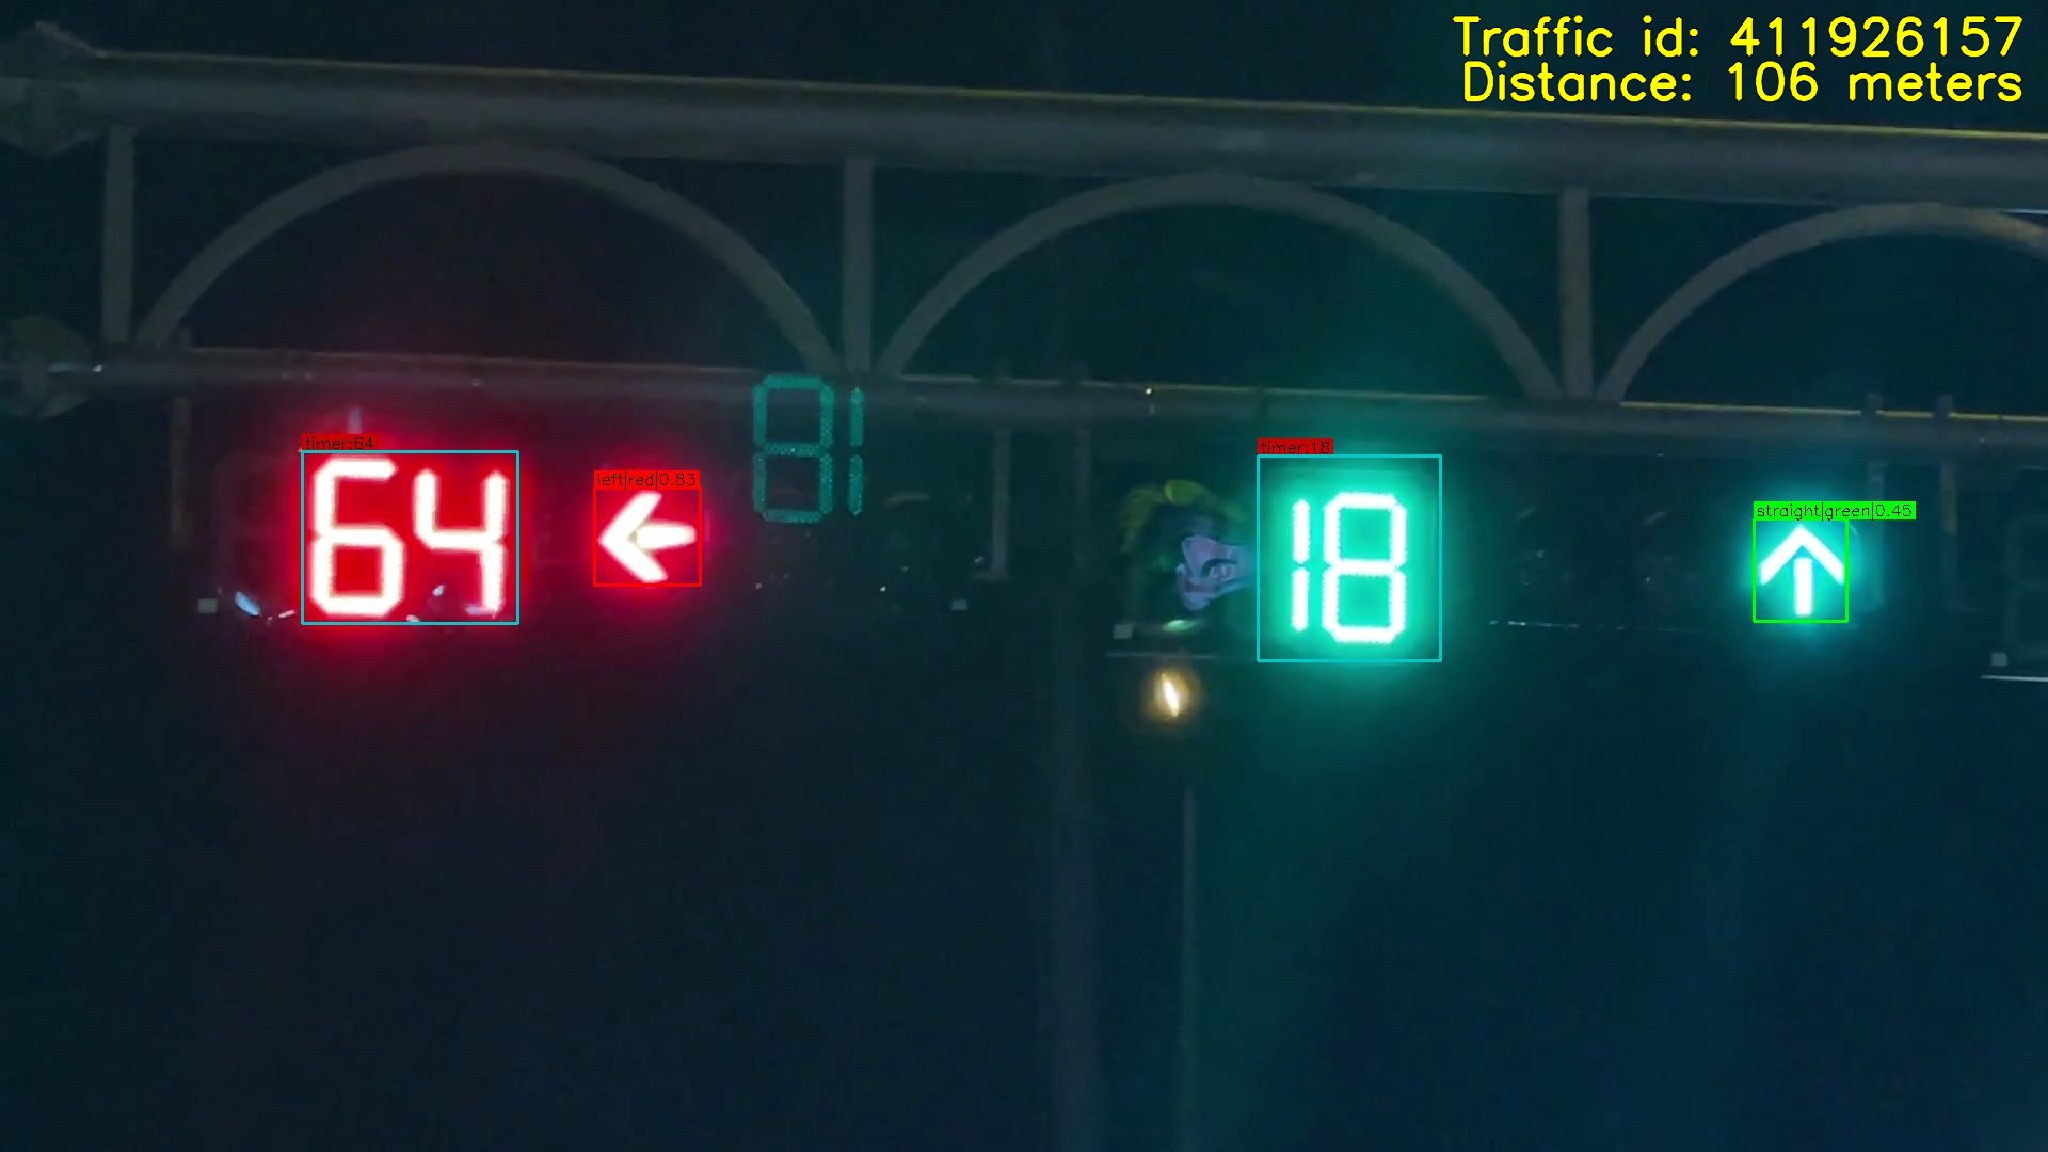
\includegraphics[width=0.75\textwidth]{Images/chapter4/result.png}
%     \vspace{0.5cm}
%     \caption{The result of prototype project}
%     \label{fig:res_project}
% \end{figure}

% Figure~\ref{fig:res_project} illustrates the experimental result obtained from the implemented prototype system. The figure shows the output generated by the ClientSensor application after receiving processed data from the ProviderSensor through the Adaptive AUTOSAR communication mechanism.

% In this experiment, the ClientSensor performs camera-based traffic light detection using the trained YOLO-MobileNet model. Detected traffic lights are highlighted with bounding boxes, and each detection is annotated with the corresponding class label and confidence score, such as red, yellow, and green signal states. The visualization demonstrates that the system is capable of identifying multiple traffic light instances within a single frame and distinguishing different signal colors under indoor test conditions.

% The execution logs displayed in the terminal confirm the end-to-end data flow within the Adaptive AUTOSAR environment. The ProviderSensor successfully publishes processed sensor data, which is then received and consumed by the ClientSensor via SOME/IP with transport protocol (SOME/IP-TP). The logs indicate correct service discovery, data transmission, and event handling between the two applications. Furthermore, the generated output image is stored locally, verifying that the perception results are correctly transferred and processed at the application level.

% Overall, this result validates the functional correctness of the prototype, demonstrating successful integration of deep learning–based perception with Adaptive AUTOSAR service-oriented communication. While the experiment is conducted in a controlled environment and does not represent full automotive deployment conditions, it confirms the feasibility of the proposed architecture and provides a solid foundation for further system optimization and real-world validation.

\subsection{Experimental Setup}
To evaluate the end-to-end functionality of the proposed ADAS architecture followed by the Figure~\ref{fig:archDesign_project}, a hardware-in-the-loop (HIL) experiment was conducted, as previously illustrated in Figure~\ref{fig:hw_arch} in Chapter 2. The setup was designed to simulate a practical in-vehicle network. Specifically, a Raspberry Pi 5 was utilized as the edge computing node to run the Provider application, which handles heavy tasks such as model inference and sensor data collection. A standard USB UVC webcam was connected to capture real-time video streams, while a GPS module supplied accurate vehicle positioning data via a UART interface.
To create a realistic distributed environment, the Client application and the visualization Human-Machine Interface (HMI) were hosted on a separate monitoring computer. This machine was connected to the Raspberry Pi 5 over a Local Area Network (LAN). This separation is important because it ensures that the edge node's processing power is dedicated entirely to AI inference, rather than displaying graphics. 

Furthermore, the overall effectiveness of this setup relies on well-trained perception models. The specific datasets and training configurations used to develop the YOLO26-MobileNetV4 model and the lightweight multi-head CNN timer detector are discussed in detail in Section~\ref{sub:datasetYolo} and Section~\ref{sec:dataCNN}, respectively.

\subsection{System Evaluation}
\begin{figure}[H]
    \centering
    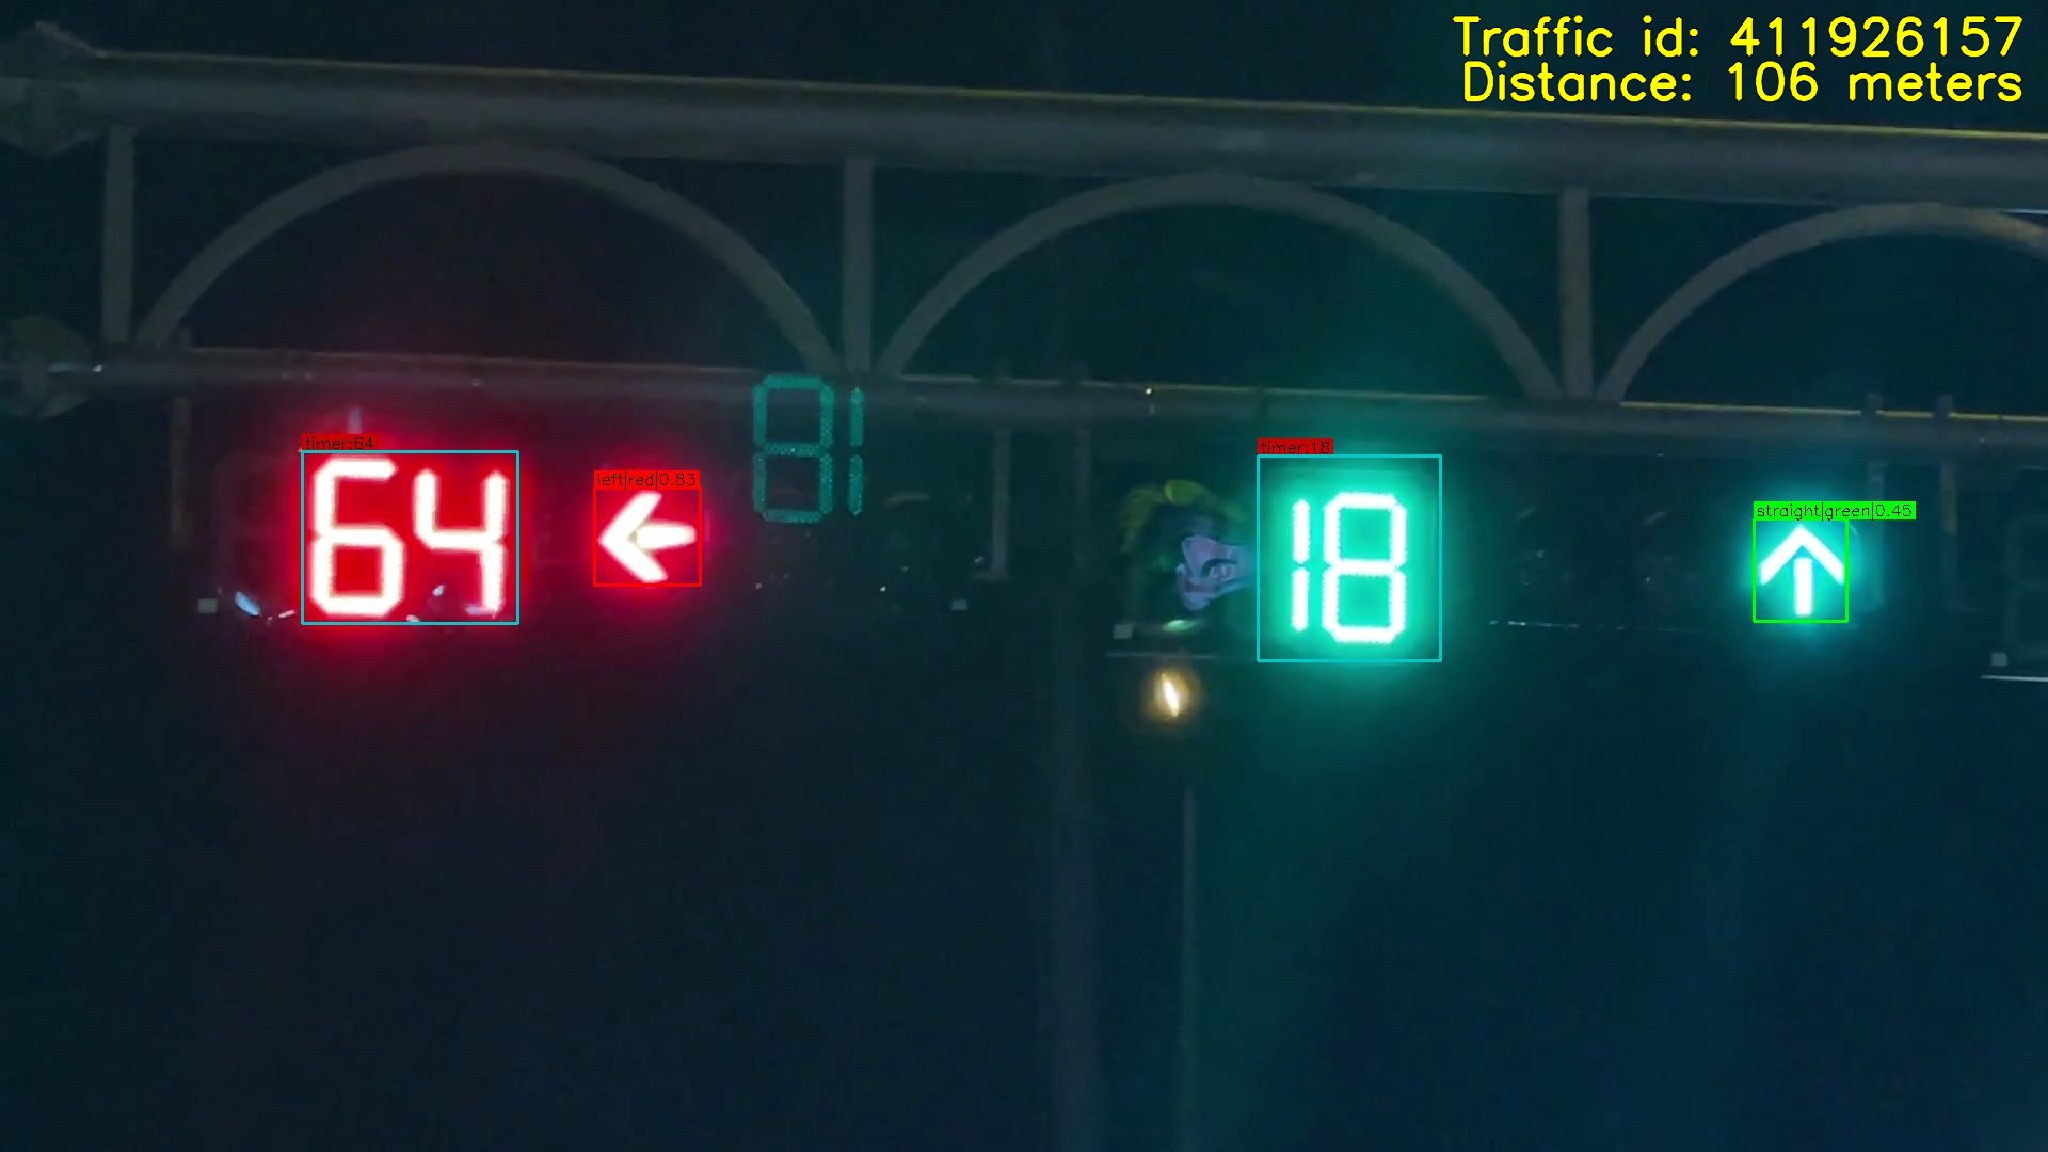
\includegraphics[width=0.75\textwidth]{Images/chapter4/result.png}
    \vspace{0.5cm}
    \caption{Prototype output displayed by the HMI/monitor}
    \label{fig:res_project}
\end{figure}

Figure~\ref{fig:res_project} presents the final visualization produced by the prototype. The monitoring HMI successfully received the data stream from the Client application over the TCP connection. The overlay in the upper-right corner reflects the traffic-light node metadata extracted from the DDS payload, correctly identifying \texttt{Traffic id: 411926157} at a \texttt{Distance: 106 meters}.

During execution, the Provider's perception pipeline successfully captured the camera frame, recognized the traffic light states, and annotated the image. The output highlights a red right-turn signal with a countdown of \texttt{64} seconds and a green straight signal with \texttt{18} seconds remaining. The seamless presentation of both the annotated image and the corresponding GPS metadata confirms that the \texttt{GpsJpegWireHeader} parsing logic functions correctly on the Client side. 

Furthermore, the successful display verifies the reliability of the underlying communication architecture. The \texttt{CycloneDDS-CXX} middleware managed the service discovery and the transportation of the \texttt{imageDataEvent} without observable payload corruption. The experiment demonstrates that the combination of edge-based perception, DDS-driven data distribution, and TCP-based visualization can sustain the required data flow for an ADAS prototype without relying on generic system boilerplates.

With the technical implementations and methodological frameworks thoroughly detailed and validated in Chapter 4, the primary objectives of this research have been addressed. Transitioning into Chapter 5, the focus will shift towards a final synthesis of the project. The upcoming chapter will offer a conclusive summary of the findings, reflect on the practical implications of the developed ADAS system, and propose viable recommendations for future enhancements.
\newpage
% \chapter{Conclusion and Future Enhancement of Project}

% This chapter presents a comprehensive evaluation of the proposed project and discusses potential directions for future enhancement. The evaluation focuses on both technical and system-level aspects, including lessons learned during development and the challenges encountered throughout the project lifecycle. Based on these insights, several future improvement directions are proposed to enhance system performance, scalability, robustness, and industrial applicability.

% \section{Conclusion}

% The proposed project demonstrates the feasibility of implementing an AI-based red-light warning system within an Adaptive AUTOSAR architecture. By integrating a deep learning–based traffic light detection model with a service-oriented automotive software framework, the project bridges the gap between perception algorithms and automotive-grade system design. The evaluation highlights the strengths of the implemented prototype, as well as the limitations that must be addressed for real-world deployment.

% From a functional perspective, the system successfully detects traffic lights from camera input, classifies signal states, and provides warning information to the client application through Adaptive AUTOSAR communication mechanisms. The modular architecture enables clear separation between perception, communication, and application logic, which improves maintainability and extensibility. Furthermore, the use of Adaptive AUTOSAR allows dynamic application management and service discovery, which are essential features for modern ADAS platforms.

% From a performance perspective, the prototype achieves acceptable inference latency under controlled test conditions on a Raspberry Pi-based environment. While the system is not yet optimized for automotive-grade hardware, the results indicate that lightweight deep learning models, such as YOLO26 with a MobileNet-based backbone, are suitable candidates for embedded ADAS perception tasks when combined with careful system integration.

% \subsection{Lesson Learned}

% Throughout the configuration, integration, and evaluation of the Adaptive AUTOSAR project, several important lessons were learned, spanning industrial collaboration, configuration-centric system development, and environment setup for AI-enabled ADAS applications.

% First, direct exposure to an industrial development environment provided valuable insights beyond purely academic experience. Through collaboration with PopcornSAR, the project team gained practical understanding of professional automotive software development workflows, including the use of proprietary toolchains, standardized configuration processes, and industry-oriented development practices. A key lesson was the importance of proactively initiating communication with the company, clearly presenting the technical objectives and scope of the project, and formally requesting access to licenses and development tools. This process required not only technical competence but also the ability to articulate system architecture, expected outcomes, and research value in a structured and professional manner. Working with an international industrial partner further emphasized the role of effective communication, responsiveness, and accountability in collaborative engineering projects.

% Second, the configuration-centric development paradigm of Adaptive AUTOSAR was identified as a foundational factor in system correctness and maintainability. Unlike traditional implementation-driven development, Adaptive AUTOSAR requires explicit definition and coordination of system artefacts, including machines, software clusters, service interfaces, executables, and deployment descriptions, before runtime behavior can be realized. This project demonstrates that incomplete or inconsistent configurations at the system design or machine design level frequently result in runtime execution issues that cannot be resolved solely through application-level debugging. Consequently, configuration planning, validation, and traceability must be treated as first-class engineering activities, on par with software implementation.

% Third, the strict separation between design, implementation, and deployment phases introduces both clarity and complexity into the development workflow. The Adaptive AUTOSAR methodology enforces incremental refinement of artefacts and explicit mapping between abstract system design and concrete executable deployment. While this separation improves scalability and long-term maintainability, it also requires a disciplined configuration mindset. Changes in service interfaces, execution states, or deployment mappings may propagate across multiple configuration layers. This project highlights the necessity of maintaining consistency across system design artefacts, application configurations, and machine manifests to ensure reliable and predictable system behavior.

% Fourth, integrating AI components into an Adaptive AUTOSAR environment requires careful alignment between machine learning workflows and automotive configuration processes. The configuration and training of the YOLOv26-MobileNetV4 model, followed by its integration through the LiteRT framework, revealed that AI models cannot be treated as standalone binaries. Instead, their runtime dependencies, resource requirements, and compatibility with the target operating system and middleware must be explicitly addressed during system configuration. The cross-compilation and deployment process underscores the importance of early consideration of framework compatibility to avoid integration bottlenecks in later development stages.

% Fifth, the use of a Docker-based development environment significantly improved reproducibility and consistency during configuration and integration. Encapsulating toolchains, dependencies, and runtime environments enabled efficient experimentation and reduced configuration drift across development stages. However, this project also demonstrates that container-based environments abstract away certain hardware-specific characteristics, such as hardware acceleration and memory hierarchy. As a result, configuration decisions validated in Docker may require reassessment when transitioning to automotive-grade hardware platforms. This reinforces the role of Docker as a development and validation tool rather than a final deployment reference.

% Finally, the Adaptive AUTOSAR methodology promotes a system-level perspective that fundamentally reshapes the development of ADAS applications. Rather than focusing solely on algorithm performance or application logic, developers must reason about execution management, service-oriented communication, and deployment constraints as integral design concerns. This project confirms that successful ADAS development within an Adaptive AUTOSAR framework depends on mastering configuration workflows and understanding how software artefacts interact dynamically at runtime.

% Overall, these lessons demonstrate that effective ADAS development is the result of both strong industrial collaboration and rigorous configuration management. Configuration is not merely a preparatory step but a foundational element that enables scalability, maintainability, and reliable integration of advanced AI functionalities. Insufficient understanding of configuration workflows or industrial development practices can undermine system reliability, regardless of algorithmic performance.


% \subsection{Challenges}

% Despite the successful implementation of the prototype, several key challenges were encountered that are primarily related to deployment maturity, communication architecture, and practical applicability of the proposed system.

% The first challenge concerns the Linux environment because of non RTOS. nên là mặc dù max spike có giảm đáng kể khi đổi yolov26n gốc sang yolo26n-mobilenetv4 nhưng mà vẫn cao hơn xấp xỉ 44,8\% dựa theo bảng \ref{tab:model_eval} đã so sánh

% The second challenge relates multithread vẫn còn bị tranh chấp ở process trong màn hình và process xử lý ảnh 4 cores ở provider sensor.

% The third challenge concerns vẫn chưa có thuật toán tối ưu môi trường trong điều kiện sáng tối, mưa hay nắng, chỉ đơn giản là train trên tập thư viện của ultralytics mà không qua thuật toán cơ bản xử lý ảnh

% Overall, these challenges indicate that the current system represents an early-stage prototype. Addressing deployment maturity, adopting DDS-based communication, and refining the use case toward more practical driving scenarios are necessary steps for advancing the system toward a realistic and production-ready ADAS implementation.


% \section{Future Work}

% Based on the identified challenges and evaluation results, several future research and development directions are proposed. These future works are structured to directly address the limitations discussed in the previous section and to gradually advance the system toward a more realistic and production-ready ADAS implementation.

% \subsection{Phát triển hệ thống này trên QNX}

% Việc phát triển trên hệ thống này sẽ tránh được spike của model trong lúc inference, làm tăng tốc độ của model --> cải thiện fps

% \subsection{Xử lý sâu điều kiện sáng tối bằng những thuật toán cơ bản khác}

% % TODO

% Overall, this infrastructure-assisted and event-driven design eliminates the need for impractical long-distance visual detection, reduces computational and sensor costs, and improves feasibility for real-world ADAS deployment. By leveraging Adaptive AUTOSAR services for data integration, execution control, and application triggering, the refined use case remains tightly coupled to the proposed prototype while addressing its key practical limitations.


\chapter{Conclusion and Future Enhancement of Project}

Finally, this report will present a comprehensive evaluation of the proposed project and discusses potential directions for future enhancement. The evaluation focuses on both technical and system-level aspects, including lessons learned during development and the challenges encountered throughout the project lifecycle. Based on these insights, several future improvement directions are proposed to enhance system performance, scalability, robustness, and industrial applicability.

\section{Conclusion}

The proposed project demonstrates the feasibility of implementing an AI-based red-light warning system within an Adaptive AUTOSAR architecture. By integrating a deep learning–based traffic light detection model with a service-oriented automotive software framework, the project bridges the gap between perception algorithms and automotive-grade system design. The evaluation highlights the strengths of the implemented prototype, as well as the limitations that must be addressed for real-world deployment.

From a functional perspective, the system successfully detects traffic lights from camera input, classifies signal states, and provides warning information to the client application through Adaptive AUTOSAR communication mechanisms. The modular architecture enables clear separation between perception, communication, and application logic, which improves maintainability and extensibility. Furthermore, the use of Adaptive AUTOSAR allows dynamic application management and service discovery, which are essential features for modern ADAS platforms.

From a performance perspective, the prototype achieves acceptable inference latency under controlled test conditions on a Raspberry Pi-based environment. While the system is not yet optimized for automotive-grade hardware, the results indicate that lightweight deep learning models, such as YOLO26 with a MobileNet-based backbone, are suitable candidates for embedded ADAS perception tasks when combined with careful system integration.

\subsection{Lesson Learned}

Throughout the configuration, integration, and evaluation of the Adaptive AUTOSAR project, several important lessons were learned, spanning industrial collaboration, configuration-centric system development, and environment setup for AI-enabled ADAS applications.

First, direct exposure to an industrial development environment provided valuable insights beyond purely academic experience. Through collaboration with PopcornSAR, the project team gained practical understanding of professional automotive software development workflows, including the use of proprietary toolchains, standardized configuration processes, and industry-oriented development practices. A key lesson was the importance of proactively initiating communication with the company, clearly presenting the technical objectives and scope of the project, and formally requesting access to licenses and development tools. This process required not only technical competence but also the ability to articulate system architecture, expected outcomes, and research value in a structured and professional manner. Working with an international industrial partner further emphasized the role of effective communication, responsiveness, and accountability in collaborative engineering projects.

Second, the configuration-centric development paradigm of Adaptive AUTOSAR was identified as a foundational factor in system correctness and maintainability. Unlike traditional implementation-driven development, Adaptive AUTOSAR requires explicit definition and coordination of system artefacts, including machines, software clusters, service interfaces, executables, and deployment descriptions, before runtime behavior can be realized. This project demonstrates that incomplete or inconsistent configurations at the system design or machine design level frequently result in runtime execution issues that cannot be resolved solely through application-level debugging. Consequently, configuration planning, validation, and traceability must be treated as first-class engineering activities, on par with software implementation.

Third, the strict separation between design, implementation, and deployment phases introduces both clarity and complexity into the development workflow. The Adaptive AUTOSAR methodology enforces incremental refinement of artefacts and explicit mapping between abstract system design and concrete executable deployment. While this separation improves scalability and long-term maintainability, it also requires a disciplined configuration mindset. Changes in service interfaces, execution states, or deployment mappings may propagate across multiple configuration layers. This project highlights the necessity of maintaining consistency across system design artefacts, application configurations, and machine manifests to ensure reliable and predictable system behavior.

Fourth, integrating AI components into an Adaptive AUTOSAR environment requires careful alignment between machine learning workflows and automotive configuration processes. The configuration and training of the YOLOv26-MobileNetV4 model, followed by its integration through the LiteRT framework, revealed that AI models cannot be treated as standalone binaries. Instead, their runtime dependencies, resource requirements, and compatibility with the target operating system and middleware must be explicitly addressed during system configuration. The cross-compilation and deployment process underscores the importance of early consideration of framework compatibility to avoid integration bottlenecks in later development stages.

Fifth, the use of a Docker-based development environment significantly improved reproducibility and consistency during configuration and integration. Encapsulating toolchains, dependencies, and runtime environments enabled efficient experimentation and reduced configuration drift across development stages. However, this project also demonstrates that container-based environments abstract away certain hardware-specific characteristics, such as hardware acceleration and memory hierarchy. As a result, configuration decisions validated in Docker may require reassessment when transitioning to automotive-grade hardware platforms. This reinforces the role of Docker as a development and validation tool rather than a final deployment reference.

Finally, the Adaptive AUTOSAR methodology promotes a system-level perspective that fundamentally reshapes the development of ADAS applications. Rather than focusing solely on algorithm performance or application logic, developers must reason about execution management, service-oriented communication, and deployment constraints as integral design concerns. This project confirms that successful ADAS development within an Adaptive AUTOSAR framework depends on mastering configuration workflows and understanding how software artefacts interact dynamically at runtime.

Overall, these lessons demonstrate that effective ADAS development is the result of both strong industrial collaboration and rigorous configuration management. Configuration is not merely a preparatory step but a foundational element that enables scalability, maintainability, and reliable integration of advanced AI functionalities. Insufficient understanding of configuration workflows or industrial development practices can undermine system reliability, regardless of algorithmic performance.


\subsection{Challenges}

Despite the successful implementation of the prototype, several key challenges were encountered that are primarily related to runtime determinism, resource contention, and perception robustness under practical driving conditions.

The first challenge concerns the use of a standard Linux environment instead of a real-time operating system. Since Linux is not configured as an RTOS in this prototype, inference and communication tasks are still affected by scheduler jitter, background services, and non-deterministic process execution. Although the maximum latency spike was significantly reduced after replacing the original YOLOv26n model with the YOLOv26n-MobileNetV4 variant, the maximum spike remains approximately 44.8\% higher than the average latency according to the comparison shown in Table~\ref{tab:model_eval}. This indicates that model optimization alone is not sufficient to guarantee deterministic execution for safety-oriented ADAS applications.

The second challenge is related to multithreaded execution and CPU resource contention. The Provider Sensor performs camera capture, AI inference, GPS processing, image encoding, and DDS publishing, while the display process also requires CPU time for TCP reception, JPEG decoding, rendering, and overlay generation. Even though CPU affinity is applied to separate the Provider processing cores from the display core, contention can still occur between image-processing workloads, memory access, operating-system scheduling, and inter-process communication. This issue can reduce frame-rate stability and introduce occasional delays in the end-to-end pipeline.

The third challenge concerns perception robustness under diverse environmental conditions. The current model is mainly trained using datasets prepared through the Ultralytics training workflow, while the image-processing pipeline does not yet include dedicated enhancement algorithms for difficult lighting and weather conditions. As a result, variations such as low light, strong sunlight, shadows, rain, glare, or motion blur may reduce detection accuracy, color classification reliability, and OCR performance. In particular, HSV-based color classification and timer recognition can become unstable if the input image quality changes significantly from the training and testing conditions.

Overall, these challenges indicate that the current system represents an early-stage prototype. Improving runtime determinism, reducing resource contention, and strengthening perception robustness under real-world environmental conditions are necessary steps for advancing the system toward a realistic and production-ready ADAS implementation.

The conclusions above summarize both the achievements and the remaining limitations of the proposed prototype. These limitations are not isolated issues, but rather indicate the next technical steps required to improve the system beyond a proof-of-concept implementation. Therefore, the following subsection outlines future work directions that directly extend the findings from the evaluation and challenges.


\section{Future Work}

Based on the identified challenges and evaluation results, several future research and development directions are proposed. These future works are structured to directly address the limitations discussed in the previous section and to gradually advance the system toward a more realistic and production-ready ADAS implementation.

\subsection{Deploying the System on QNX}

A key future direction is to migrate the prototype from the current Linux-based environment to QNX or another automotive-grade real-time operating system. QNX provides deterministic scheduling, stronger process isolation, and real-time execution guarantees, which are important for reducing inference latency spikes and improving the stability of the perception pipeline. By controlling task priorities, CPU scheduling, and inter-process communication more strictly, the system can reduce the impact of background processes and operating-system jitter on AI inference.

Deploying the system on QNX is expected to improve frame-rate stability and reduce the difference between average latency and worst-case latency. This is especially important for ADAS applications, where occasional latency spikes may be more critical than average inference time. In addition, QNX is widely used in automotive platforms, making this migration a necessary step toward evaluating the prototype under conditions closer to industrial deployment.

\subsection{Improving Robustness under Lighting and Weather Conditions}

Another important future enhancement is to strengthen the perception pipeline under challenging environmental conditions. The current implementation mainly relies on the trained YOLOv26n-MobileNetV4 model and a basic HSV-based color classification pipeline. Future work should introduce additional classical image-processing and enhancement techniques to improve input quality before detection, color classification, and OCR are performed.

Potential improvements include brightness and contrast normalization, gamma correction, histogram equalization, glare reduction, shadow handling, denoising, and adaptive thresholding for low-light or high-exposure scenes. For rainy or noisy environments, preprocessing techniques such as image deblurring, temporal smoothing, and region-based filtering may improve both traffic light detection and timer OCR reliability. These methods can be combined with data augmentation during model training so that the AI model and the image-processing pipeline are both more robust to variations in illumination, weather, and camera quality.

Overall, these future enhancements directly address the main limitations observed in the prototype. Migrating to QNX would improve runtime determinism and reduce latency spikes, while deeper environmental image processing would improve perception reliability in realistic driving scenarios. Together, these improvements would move the system closer to an automotive-grade ADAS implementation.

\newpage
%-------------OUTRO----------------%
% \input{Outro/Reference.tex}
\nocite{*}
\bibliographystyle{IEEEtran}
\bibliography{references}

\newpage
\chapter*{Appendix: Research Paper: YOLOv11n-MobileNetV4 for Edge AI in Adaptive AUTOSAR}
\phantomsection
\label{chap:append}

\addcontentsline{toc}{chapter}{Appendix: Research Paper}

Following the successful completion of the project, a comprehensive research paper was submitted to the IEEE Sensors Applications Symposium (SAS) 2026, focusing on Edge AI. The manuscript presents a lightweight framework for real-time traffic light detection, seamlessly integrated into the AUTOSAR Adaptive Platform for ADAS applications.

To address the strict latency and resource constraints of edge sensor nodes, the paper proposes a highly optimized YOLO11-MobileNetV4 architecture using post-training quantization for efficient CPU-only inference. Implemented as an SOA-compliant C++ Adaptive Application, the pipeline proves the viability of accelerator-free edge computing. Experimental results demonstrate that the proposed model achieves a real-time throughput of approximately 27 frames per second at an input resolution of $320 \times 320$ on standard embedded hardware. It delivers a 2.5$\times$ speedup over the YOLO11n baseline and outperforms YOLO8n and SSD-MobileNetV3 in inference speed, while maintaining superior accuracy (mAP@50) compared to the SSD baseline.

The original manuscript for this IEEE submission is appended below, serving as a formal academic validation of the proposed ADAS development methodology.

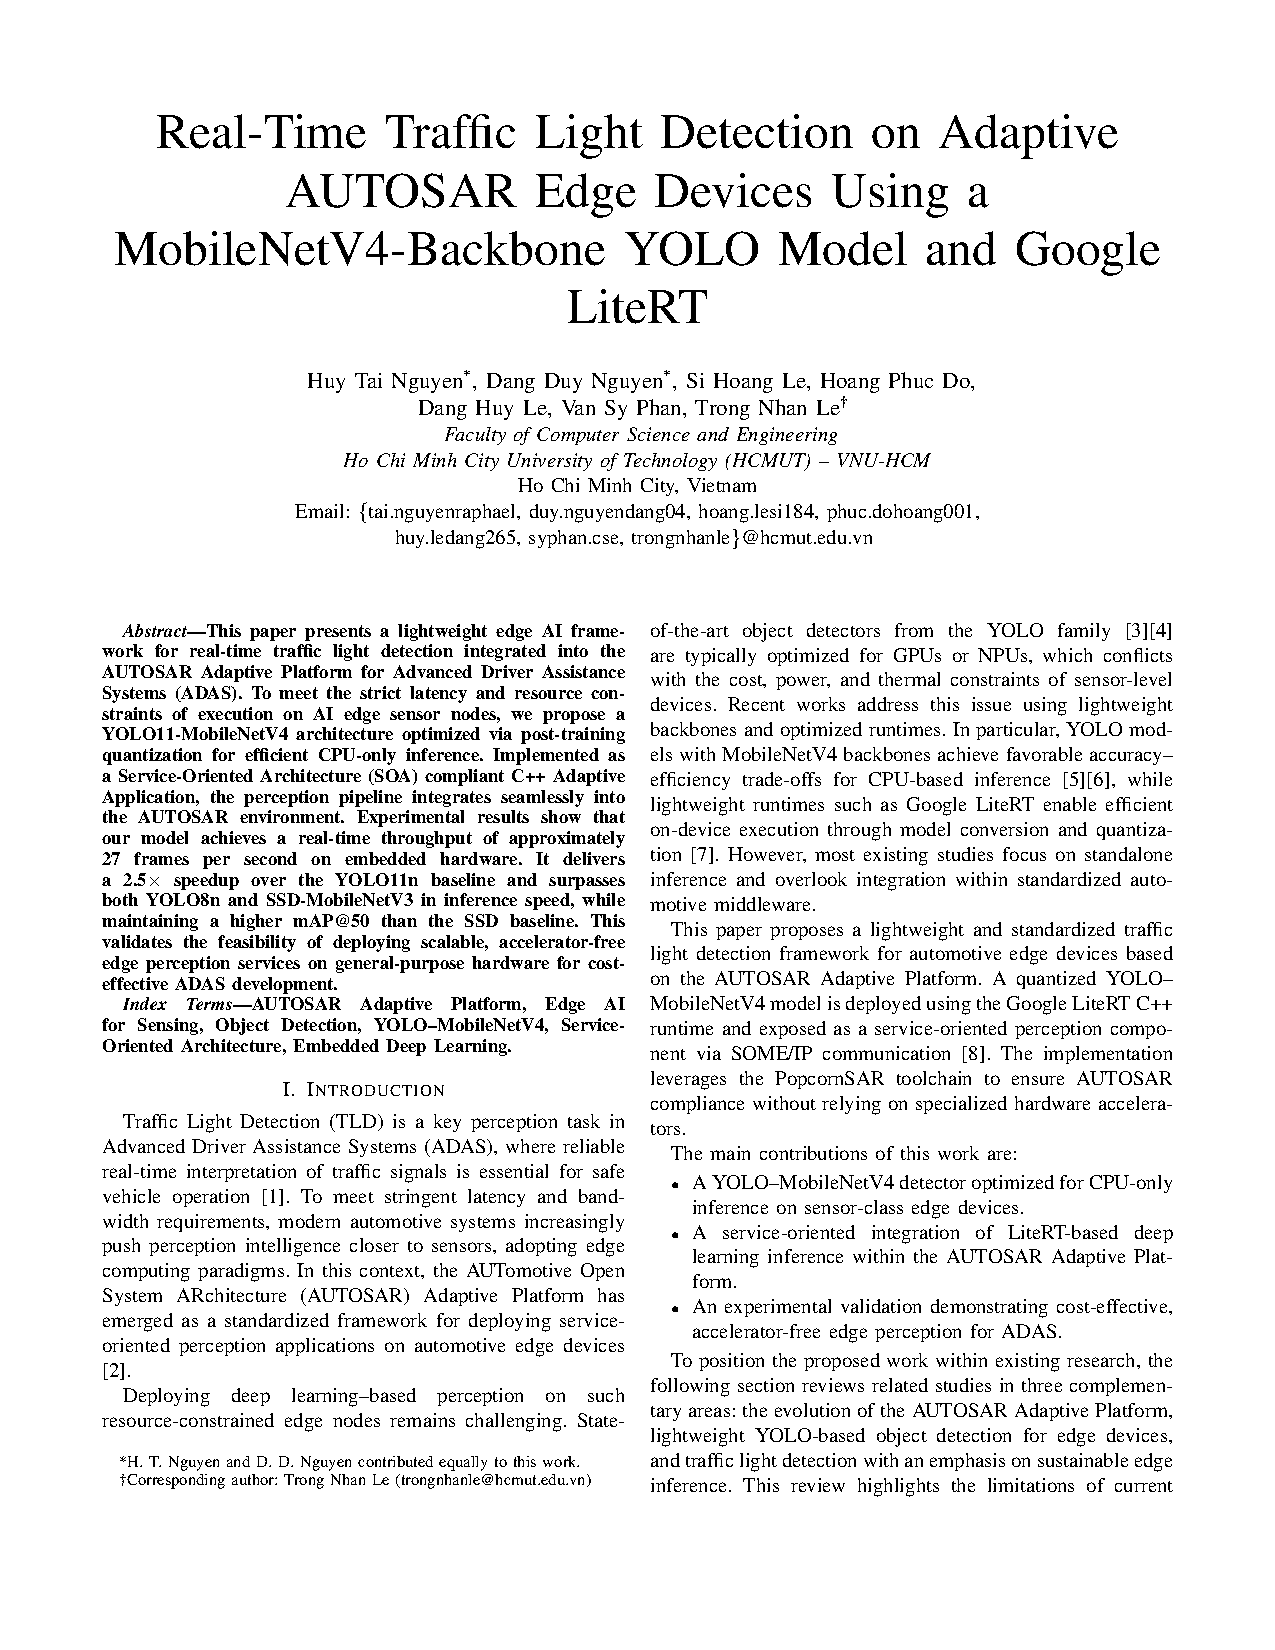
\includepdf[pages=-, scale=0.85, pagecommand={}]{YOLO_MobilenetV4_LiteRT_AUTOSAR_paper.pdf}

\end{document}


